% Options for packages loaded elsewhere
\PassOptionsToPackage{unicode}{hyperref}
\PassOptionsToPackage{hyphens}{url}
\PassOptionsToPackage{dvipsnames,svgnames,x11names}{xcolor}
%
\documentclass[
  letterpaper,
]{svmono}

\usepackage{amsmath,amssymb}
\usepackage{iftex}
\ifPDFTeX
  \usepackage[T1]{fontenc}
  \usepackage[utf8]{inputenc}
  \usepackage{textcomp} % provide euro and other symbols
\else % if luatex or xetex
  \usepackage{unicode-math}
  \defaultfontfeatures{Scale=MatchLowercase}
  \defaultfontfeatures[\rmfamily]{Ligatures=TeX,Scale=1}
\fi
\usepackage{lmodern}
\ifPDFTeX\else  
    % xetex/luatex font selection
    \setmainfont[]{Palatino}
    \setmonofont[]{Inconsolata}
\fi
% Use upquote if available, for straight quotes in verbatim environments
\IfFileExists{upquote.sty}{\usepackage{upquote}}{}
\IfFileExists{microtype.sty}{% use microtype if available
  \usepackage[]{microtype}
  \UseMicrotypeSet[protrusion]{basicmath} % disable protrusion for tt fonts
}{}
\makeatletter
\@ifundefined{KOMAClassName}{% if non-KOMA class
  \IfFileExists{parskip.sty}{%
    \usepackage{parskip}
  }{% else
    \setlength{\parindent}{0pt}
    \setlength{\parskip}{6pt plus 2pt minus 1pt}}
}{% if KOMA class
  \KOMAoptions{parskip=half}}
\makeatother
\usepackage{xcolor}
\setlength{\emergencystretch}{3em} % prevent overfull lines
\setcounter{secnumdepth}{5}
% Make \paragraph and \subparagraph free-standing
\makeatletter
\ifx\paragraph\undefined\else
  \let\oldparagraph\paragraph
  \renewcommand{\paragraph}{
    \@ifstar
      \xxxParagraphStar
      \xxxParagraphNoStar
  }
  \newcommand{\xxxParagraphStar}[1]{\oldparagraph*{#1}\mbox{}}
  \newcommand{\xxxParagraphNoStar}[1]{\oldparagraph{#1}\mbox{}}
\fi
\ifx\subparagraph\undefined\else
  \let\oldsubparagraph\subparagraph
  \renewcommand{\subparagraph}{
    \@ifstar
      \xxxSubParagraphStar
      \xxxSubParagraphNoStar
  }
  \newcommand{\xxxSubParagraphStar}[1]{\oldsubparagraph*{#1}\mbox{}}
  \newcommand{\xxxSubParagraphNoStar}[1]{\oldsubparagraph{#1}\mbox{}}
\fi
\makeatother

\usepackage{color}
\usepackage{fancyvrb}
\newcommand{\VerbBar}{|}
\newcommand{\VERB}{\Verb[commandchars=\\\{\}]}
\DefineVerbatimEnvironment{Highlighting}{Verbatim}{commandchars=\\\{\}}
% Add ',fontsize=\small' for more characters per line
\usepackage{framed}
\definecolor{shadecolor}{RGB}{241,243,245}
\newenvironment{Shaded}{\begin{snugshade}}{\end{snugshade}}
\newcommand{\AlertTok}[1]{\textcolor[rgb]{0.68,0.00,0.00}{#1}}
\newcommand{\AnnotationTok}[1]{\textcolor[rgb]{0.37,0.37,0.37}{#1}}
\newcommand{\AttributeTok}[1]{\textcolor[rgb]{0.40,0.45,0.13}{#1}}
\newcommand{\BaseNTok}[1]{\textcolor[rgb]{0.68,0.00,0.00}{#1}}
\newcommand{\BuiltInTok}[1]{\textcolor[rgb]{0.00,0.23,0.31}{#1}}
\newcommand{\CharTok}[1]{\textcolor[rgb]{0.13,0.47,0.30}{#1}}
\newcommand{\CommentTok}[1]{\textcolor[rgb]{0.37,0.37,0.37}{#1}}
\newcommand{\CommentVarTok}[1]{\textcolor[rgb]{0.37,0.37,0.37}{\textit{#1}}}
\newcommand{\ConstantTok}[1]{\textcolor[rgb]{0.56,0.35,0.01}{#1}}
\newcommand{\ControlFlowTok}[1]{\textcolor[rgb]{0.00,0.23,0.31}{\textbf{#1}}}
\newcommand{\DataTypeTok}[1]{\textcolor[rgb]{0.68,0.00,0.00}{#1}}
\newcommand{\DecValTok}[1]{\textcolor[rgb]{0.68,0.00,0.00}{#1}}
\newcommand{\DocumentationTok}[1]{\textcolor[rgb]{0.37,0.37,0.37}{\textit{#1}}}
\newcommand{\ErrorTok}[1]{\textcolor[rgb]{0.68,0.00,0.00}{#1}}
\newcommand{\ExtensionTok}[1]{\textcolor[rgb]{0.00,0.23,0.31}{#1}}
\newcommand{\FloatTok}[1]{\textcolor[rgb]{0.68,0.00,0.00}{#1}}
\newcommand{\FunctionTok}[1]{\textcolor[rgb]{0.28,0.35,0.67}{#1}}
\newcommand{\ImportTok}[1]{\textcolor[rgb]{0.00,0.46,0.62}{#1}}
\newcommand{\InformationTok}[1]{\textcolor[rgb]{0.37,0.37,0.37}{#1}}
\newcommand{\KeywordTok}[1]{\textcolor[rgb]{0.00,0.23,0.31}{\textbf{#1}}}
\newcommand{\NormalTok}[1]{\textcolor[rgb]{0.00,0.23,0.31}{#1}}
\newcommand{\OperatorTok}[1]{\textcolor[rgb]{0.37,0.37,0.37}{#1}}
\newcommand{\OtherTok}[1]{\textcolor[rgb]{0.00,0.23,0.31}{#1}}
\newcommand{\PreprocessorTok}[1]{\textcolor[rgb]{0.68,0.00,0.00}{#1}}
\newcommand{\RegionMarkerTok}[1]{\textcolor[rgb]{0.00,0.23,0.31}{#1}}
\newcommand{\SpecialCharTok}[1]{\textcolor[rgb]{0.37,0.37,0.37}{#1}}
\newcommand{\SpecialStringTok}[1]{\textcolor[rgb]{0.13,0.47,0.30}{#1}}
\newcommand{\StringTok}[1]{\textcolor[rgb]{0.13,0.47,0.30}{#1}}
\newcommand{\VariableTok}[1]{\textcolor[rgb]{0.07,0.07,0.07}{#1}}
\newcommand{\VerbatimStringTok}[1]{\textcolor[rgb]{0.13,0.47,0.30}{#1}}
\newcommand{\WarningTok}[1]{\textcolor[rgb]{0.37,0.37,0.37}{\textit{#1}}}

\providecommand{\tightlist}{%
  \setlength{\itemsep}{0pt}\setlength{\parskip}{0pt}}\usepackage{longtable,booktabs,array}
\usepackage{calc} % for calculating minipage widths
% Correct order of tables after \paragraph or \subparagraph
\usepackage{etoolbox}
\makeatletter
\patchcmd\longtable{\par}{\if@noskipsec\mbox{}\fi\par}{}{}
\makeatother
% Allow footnotes in longtable head/foot
\IfFileExists{footnotehyper.sty}{\usepackage{footnotehyper}}{\usepackage{footnote}}
\makesavenoteenv{longtable}
\usepackage{graphicx}
\makeatletter
\newsavebox\pandoc@box
\newcommand*\pandocbounded[1]{% scales image to fit in text height/width
  \sbox\pandoc@box{#1}%
  \Gscale@div\@tempa{\textheight}{\dimexpr\ht\pandoc@box+\dp\pandoc@box\relax}%
  \Gscale@div\@tempb{\linewidth}{\wd\pandoc@box}%
  \ifdim\@tempb\p@<\@tempa\p@\let\@tempa\@tempb\fi% select the smaller of both
  \ifdim\@tempa\p@<\p@\scalebox{\@tempa}{\usebox\pandoc@box}%
  \else\usebox{\pandoc@box}%
  \fi%
}
% Set default figure placement to htbp
\def\fps@figure{htbp}
\makeatother
% definitions for citeproc citations
\NewDocumentCommand\citeproctext{}{}
\NewDocumentCommand\citeproc{mm}{%
  \begingroup\def\citeproctext{#2}\cite{#1}\endgroup}
\makeatletter
 % allow citations to break across lines
 \let\@cite@ofmt\@firstofone
 % avoid brackets around text for \cite:
 \def\@biblabel#1{}
 \def\@cite#1#2{{#1\if@tempswa , #2\fi}}
\makeatother
\newlength{\cslhangindent}
\setlength{\cslhangindent}{1.5em}
\newlength{\csllabelwidth}
\setlength{\csllabelwidth}{3em}
\newenvironment{CSLReferences}[2] % #1 hanging-indent, #2 entry-spacing
 {\begin{list}{}{%
  \setlength{\itemindent}{0pt}
  \setlength{\leftmargin}{0pt}
  \setlength{\parsep}{0pt}
  % turn on hanging indent if param 1 is 1
  \ifodd #1
   \setlength{\leftmargin}{\cslhangindent}
   \setlength{\itemindent}{-1\cslhangindent}
  \fi
  % set entry spacing
  \setlength{\itemsep}{#2\baselineskip}}}
 {\end{list}}
\usepackage{calc}
\newcommand{\CSLBlock}[1]{\hfill\break\parbox[t]{\linewidth}{\strut\ignorespaces#1\strut}}
\newcommand{\CSLLeftMargin}[1]{\parbox[t]{\csllabelwidth}{\strut#1\strut}}
\newcommand{\CSLRightInline}[1]{\parbox[t]{\linewidth - \csllabelwidth}{\strut#1\strut}}
\newcommand{\CSLIndent}[1]{\hspace{\cslhangindent}#1}

% template.tex: Springer-compatible LaTeX header for Quarto

\usepackage{fontspec}

% Essential Springer-required fonts and packages
% \usepackage{mathptmx} % Times font (Springer default)
% \usepackage{helvet}   % Helvetica font (for sans-serif text)
% \usepackage{courier}  % Courier font (monospaced text)
% \usepackage{type1cm}  % Ensures scalable fonts (Type 1)

% Additional Springer-specific settings:
\usepackage{makeidx}  % Required for indexing
\makeindex            % Enable index generation

% For better tables
\usepackage{booktabs}

% Figures and graphics settings
\usepackage{graphicx}

% Math packages (often used in Springer books)
\usepackage{amsmath}
\usepackage{amssymb}

% Springer-specific gray boxes (optional):
\usepackage{tcolorbox}
\tcbuselibrary{listingsutf8}
\tcbset{
  boxrule=0pt,
  colback=gray!10,
  colframe=gray!40,
  sharp corners
}

\usepackage{listings}
\lstset{
  breaklines=true,
  breakatwhitespace=false,
  postbreak=\mbox{\textcolor{gray}{$\hookrightarrow$}\space},
  basicstyle=\monofont,
  columns=fullflexible,
  keepspaces=true,
  frame=single,
  xleftmargin=1em,
  tabsize=2
}


\usepackage{fvextra}
\DefineVerbatimEnvironment{Highlighting}{Verbatim}{
  breaklines=true,
  breakanywhere=true,
  fontsize=\small,
  commandchars=\\\{\}
}

\numberwithin{example}{subsection}


% Custom commands (optional):
\newcommand{\R}{\textsf{R}}
\usepackage{booktabs}
\usepackage{longtable}
\usepackage{array}
\usepackage{multirow}
\usepackage{wrapfig}
\usepackage{float}
\usepackage{colortbl}
\usepackage{pdflscape}
\usepackage{tabu}
\usepackage{threeparttable}
\usepackage{threeparttablex}
\usepackage[normalem]{ulem}
\usepackage{makecell}
\usepackage{xcolor}
\makeatletter
\@ifpackageloaded{bookmark}{}{\usepackage{bookmark}}
\makeatother
\makeatletter
\@ifpackageloaded{caption}{}{\usepackage{caption}}
\AtBeginDocument{%
\ifdefined\contentsname
  \renewcommand*\contentsname{Table of contents}
\else
  \newcommand\contentsname{Table of contents}
\fi
\ifdefined\listfigurename
  \renewcommand*\listfigurename{List of Figures}
\else
  \newcommand\listfigurename{List of Figures}
\fi
\ifdefined\listtablename
  \renewcommand*\listtablename{List of Tables}
\else
  \newcommand\listtablename{List of Tables}
\fi
\ifdefined\figurename
  \renewcommand*\figurename{Figure}
\else
  \newcommand\figurename{Figure}
\fi
\ifdefined\tablename
  \renewcommand*\tablename{Table}
\else
  \newcommand\tablename{Table}
\fi
}
\@ifpackageloaded{float}{}{\usepackage{float}}
\floatstyle{ruled}
\@ifundefined{c@chapter}{\newfloat{codelisting}{h}{lop}}{\newfloat{codelisting}{h}{lop}[chapter]}
\floatname{codelisting}{Listing}
\newcommand*\listoflistings{\listof{codelisting}{List of Listings}}
\makeatother
\makeatletter
\makeatother
\makeatletter
\@ifpackageloaded{caption}{}{\usepackage{caption}}
\@ifpackageloaded{subcaption}{}{\usepackage{subcaption}}
\makeatother

\usepackage{bookmark}

\IfFileExists{xurl.sty}{\usepackage{xurl}}{} % add URL line breaks if available
\urlstyle{same} % disable monospaced font for URLs
\hypersetup{
  pdftitle={Data Science Foundations and Machine Learning with R: From Data to Decisions},
  pdfauthor={Reza Mohammadi},
  colorlinks=true,
  linkcolor={blue},
  filecolor={Maroon},
  citecolor={Blue},
  urlcolor={Blue},
  pdfcreator={LaTeX via pandoc}}


\title{Data Science Foundations and Machine Learning with R: From Data
to Decisions}
\author{\href{https://www.uva.nl/profile/a.mohammadi}{{Reza Mohammadi}}}
\date{20 October 2025}

\begin{document}
\maketitle

\renewcommand*\contentsname{Table of contents}
{
\hypersetup{linkcolor=}
\setcounter{tocdepth}{2}
\tableofcontents
}

\bookmarksetup{startatroot}

\chapter*{}\label{section}
\addcontentsline{toc}{chapter}{}

\markboth{}{}

\bookmarksetup{startatroot}

\chapter*{Preface}\label{preface}
\addcontentsline{toc}{chapter}{Preface}

\markboth{Preface}{Preface}

\emph{Data science} is transforming how we understand the world, solve
problems, and make informed decisions. From generative AI systems such
as ChatGPT, DeepSeek, and Gemini to personalized recommendations on
streaming platforms and fraud detection in banking, data-driven
techniques are reshaping industries and everyday life. As demand grows
for professionals who can analyze and model data effectively, accessible
and rigorous educational resources are more essential than ever.

\emph{Data Science Foundations and Machine Learning with R: From Data to
Decisions} offers a hands-on introduction to this dynamic field.
Designed for readers with no prior experience in analytics or
programming, the book provides a clear, structured pathway into data
science by emphasizing conceptual understanding, practical application,
and reproducible workflows using R.

This book is intended for newcomers to data science and machine
learning, particularly those without a background in programming or
statistics. Whether you are a student, business professional, or
researcher, it offers an approachable yet academically grounded learning
experience. Drawing on my experience teaching data science at the
university level, I emphasize an applied, example-driven approach that
fosters active engagement and deep comprehension.

The motivation for this book stems from a recurring challenge I
encountered in the classroom: many of my students were eager to explore
data science but lacked resources that were both accessible and
conceptually rigorous. I saw a clear need for materials that bridge
foundational theory and meaningful application. My goal was to provide a
guided, practical learning experience, lowering the barrier to entry
without sacrificing depth, through real data and hands-on practice in R.

To support a smoother learning curve, the book adopts \emph{active
learning strategies}. Concepts are introduced progressively and
reinforced through illustrative examples, guided coding exercises, and
applied problem-solving. By working directly with authentic datasets and
practical scenarios, readers learn not only how data science tools work,
but also when and why to use them. This experiential approach fosters
lasting understanding and builds confidence in applying these skills
independently.

Rather than presenting machine learning as a purely theoretical
discipline, the book integrates annotated code, real datasets, and
structured walkthroughs throughout. Each chapter concludes with a case
study that applies the chapter's core ideas to a realistic context,
bridging the gap between theory and practice. Exercises further
reinforce learning through direct implementation in R, helping readers
develop both conceptual clarity and practical fluency.

\section*{Why This Book?}\label{why-this-book}
\addcontentsline{toc}{section}{Why This Book?}

\markright{Why This Book?}

\emph{Data science} is a rapidly evolving field that integrates machine
learning, statistical modeling, and computational tools to extract
insights from data. This book provides a structured, application-focused
introduction to data analysis and machine learning using R, a widely
adopted, open-source language known for its strengths in statistical
computing, visualization, and reproducible workflows.

Unlike many textbooks that assume prior experience with programming or
analytics, this book is designed to be \emph{accessible and hands-on}.
Concepts are introduced clearly and reinforced through real-world
examples, guided exercises, and annotated R code. This approach allows
readers to build theoretical understanding alongside practical fluency
from the outset.

With its extensive ecosystem of packages, R remains a leading tool for
data science across academic, industrial, and research settings. This
book emphasizes its practical use in solving data-driven problems. For
readers who prefer Python, a companion volume titled \emph{Data Science
Foundations and Machine Learning with Python: From Data to Decisions} is
also available from the same publisher.

\section*{Who Should Read This Book?}\label{who-should-read-this-book}
\addcontentsline{toc}{section}{Who Should Read This Book?}

\markright{Who Should Read This Book?}

This book is intended for anyone seeking to learn data science and
machine learning, particularly those new to the field. It is well-suited
for:

\begin{itemize}
\item
  Business professionals aiming to integrate data-driven decision-making
  into their work,
\item
  Students and researchers applying data analysis in academic or applied
  contexts,
\item
  Beginners with no prior experience in programming or analytics,
\item
  Readers interested in learning data science and machine learning using
  R.
\end{itemize}

It is especially appropriate for undergraduate students in programs that
emphasize quantitative reasoning, such as economics, business
administration, business economics (including specializations in finance
or organizational economics), communication science, psychology, and
STEM fields (science, technology, engineering, and mathematics). It also
supports students in Master's programs in business analytics,
econometrics, and the social sciences.

Designed for both self-study and classroom use, the book offers a
structured and practice-oriented path to applying data science
techniques in real-world settings. It serves as the reference for
courses such as \emph{Data Analytics: Machine Learning}, \emph{Data
Wrangling}, and \emph{Business Analytics} across several BSc and MSc
programs at the University of Amsterdam.

It is equally useful for professionals pursuing continuing education in
analytics, offering an accessible foundation for those looking to
strengthen their skills in a rapidly evolving data landscape.

\section*{Skills You Will Gain}\label{skills-you-will-gain}
\addcontentsline{toc}{section}{Skills You Will Gain}

\markright{Skills You Will Gain}

This book walks you through a practical and progressive journey into
data science and machine learning using R, structured around the
\emph{Data Science Workflow} (Figure \ref{fig-ch0_DSW}). Each chapter
supports both conceptual mastery and applied skill development, helping
you progress from understanding and applying core ideas to analyzing
results and evaluating solutions.

By the end of this book, you will be able to:

\begin{itemize}
\item
  \emph{Recognize and describe} the key stages of a data science
  project, from problem formulation to model evaluation;
\item
  \emph{Apply} core R programming concepts, including data structures,
  control flow, and functions, to prepare and analyze data;
\item
  \emph{Clean and transform} raw datasets by handling missing values,
  outliers, and categorical variables using best practices;
\item
  \emph{Explore and interpret} data using descriptive statistics and
  effective visualizations;
\item
  \emph{Build and tune} machine learning models for classification,
  regression, and clustering using algorithms such as k-NN, Naive Bayes,
  decision trees, neural networks, and K-means;
\item
  \emph{Assess and compare} model performance using relevant metrics
  tailored to each type of task;
\item
  \emph{Transfer and adapt} your skills to solve real-world problems in
  marketing, finance, operations, and beyond.
\end{itemize}

Each chapter integrates illustrative examples, annotated R code, and
exercises that reinforce learning through practice. Chapters conclude
with a case study that synthesizes the main concepts, guiding you in
applying techniques to authentic scenarios. This structure ensures that
by the end of the book, you are not just familiar with the tools; you
are equipped to use them thoughtfully and effectively.

\section*{Structure of This Book}\label{structure-of-this-book}
\addcontentsline{toc}{section}{Structure of This Book}

\markright{Structure of This Book}

This book is structured around the \emph{Data Science Workflow}, an
iterative framework that guides you from foundational concepts to
advanced machine learning techniques through hands-on learning. Your
journey begins in Chapter \ref{sec-ch1-intro-R}, where you will install
R, explore its syntax, and work with essential data structures. From
there, each chapter builds on the previous one, combining coding
practice with real-world case studies to help you gain both
understanding and experience.

\begin{figure}[H]

\centering{

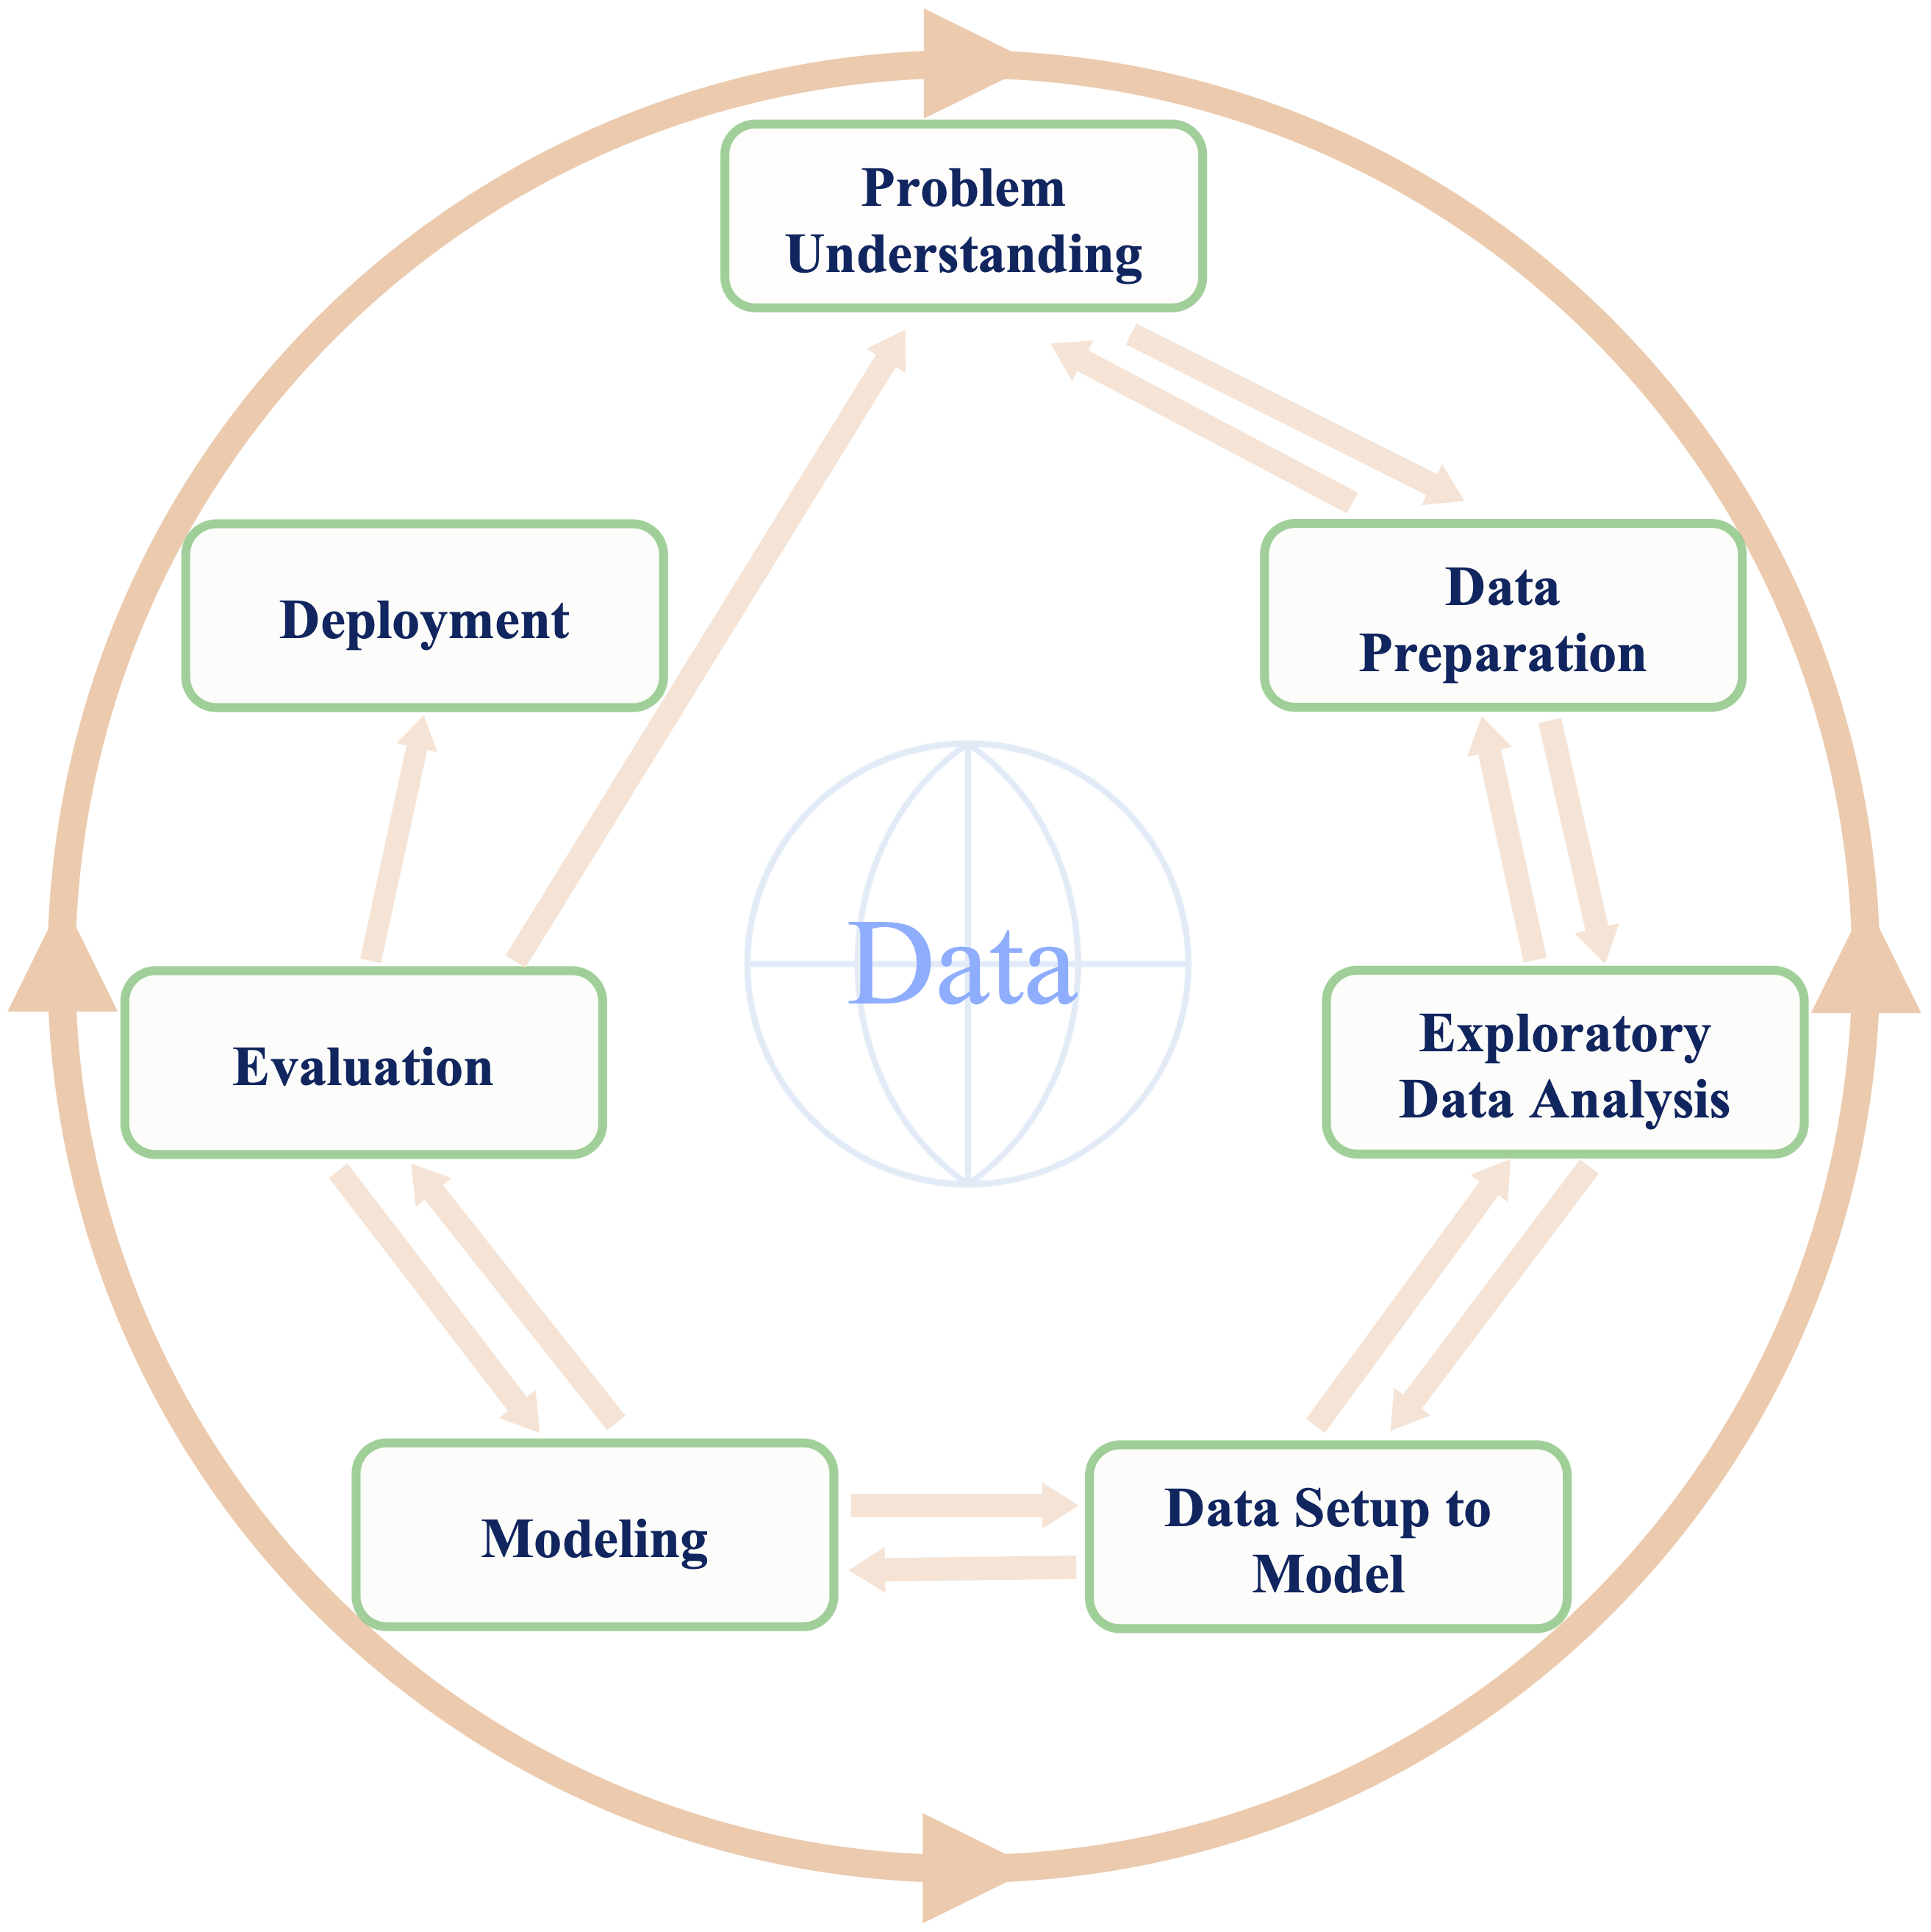
\includegraphics[width=0.7\linewidth,height=\textheight,keepaspectratio]{images/ch2_DSW.png}

}

\caption{\label{fig-ch0_DSW}The Data Science Workflow is an iterative
framework for structuring data science and machine learning projects.
Inspired by the CRISP-DM model (Cross-Industry Standard Process for Data
Mining), it supports systematic problem-solving and continuous
refinement.}

\end{figure}%

The \emph{Data Science Workflow}, introduced in Chapter
\ref{sec-ch2-intro-data-science} and illustrated in
Figure~\ref{fig-ch0_DSW}, consists of seven key stages:

\begin{enumerate}
\def\labelenumi{\arabic{enumi}.}
\item
  \emph{Problem Understanding}: Define the objective and the broader
  context (Chapter \ref{sec-ch2-intro-data-science}).
\item
  \emph{Data Preparation}: Clean, transform, and organize raw data
  (Chapter \ref{sec-ch3-data-preparation}).
\item
  \emph{Exploratory Data Analysis (EDA)}: Visualize and summarize data
  to uncover patterns (Chapter \ref{sec-ch4-EDA}).
\item
  \emph{Data Setup to Model}: Select features, partition datasets, and
  scale variables (Chapter \ref{sec-ch6-setup-data}).
\item
  \emph{Modeling}: Build and train predictive models using a range of
  machine learning algorithms (Chapters \ref{sec-ch7-classification-knn}
  to \ref{sec-ch13-clustering}).
\item
  \emph{Evaluation}: Measure model performance using appropriate metrics
  (Chapter \ref{sec-ch8-evaluation}).
\item
  \emph{Deployment}: Translate models into real-world applications.
\end{enumerate}

This workflow provides a practical and repeatable framework for tackling
data-driven problems. The chapter sequence mirrors these phases,
supporting a gradual progression from theory to implementation.

Chapter \ref{sec-ch5-statistics} also provides a concise review of key
statistical ideas, such as confidence intervals and hypothesis testing,
that support critical thinking and model interpretation.

To bridge theory and practice, each chapter concludes with a case study
that applies its core ideas to a real-world problem. These case studies
walk through the \emph{Data Science Workflow} in action: guiding you
through data preparation, model development, evaluation, and
interpretation using real datasets. The datasets, listed in Table
Table~\ref{tbl-data-table}, are available through the \textbf{liver}
package. This enables you to reproduce examples, complete exercises, and
build practical skills with minimal setup.

Each chapter ends with exercises designed to consolidate learning: from
conceptual questions and hands-on coding tasks to applied
problem-solving challenges. These help reinforce key ideas, encourage
experimentation, and build confidence in using R for data science.

\section*{How to Use This Book}\label{how-to-use-this-book}
\addcontentsline{toc}{section}{How to Use This Book}

\markright{How to Use This Book}

This book is designed for \emph{self-study, classroom instruction, and
professional learning}. You can work through the chapters sequentially
for a structured learning path or consult individual sections to focus
on specific skills or concepts.

To make the most of this book:

\begin{itemize}
\item
  \emph{Run the code} -- Execute the R code examples interactively to
  reinforce key ideas through immediate feedback and hands-on
  experience.
\item
  \emph{Solve the exercises} -- Tackle a range of questions in each
  chapter to deepen your understanding and strengthen analytical
  fluency.
\item
  \emph{Experiment with the code} -- Modify examples, test new
  parameters, and experiment with different datasets to sharpen your
  problem-solving skills.
\item
  \emph{Study the case studies} -- Use the end-of-chapter case studies
  to see the Data Science Workflow in action, from data preparation to
  model interpretation.
\item
  \emph{Use the book as a reference} -- Return to chapters as needed to
  support your projects and refresh specific techniques.
\end{itemize}

Each chapter concludes with a case study based on a real-world dataset.
These walk through the complete Data Science Workflow: preparation,
modeling, evaluation, and interpretation, helping you consolidate
learning and apply techniques in realistic analytical contexts.

This book also supports collaborative learning. Working through
exercises and case studies in pairs or small groups can spark
discussion, deepen understanding, and foster diverse perspectives,
especially in classroom and workshop environments.

The book has been successfully used in data science courses at the
University of Amsterdam and is well-suited for academic programs and
professional training. Whether you are an independent learner,
instructor, or practitioner, it offers a flexible and structured path to
mastering essential tools and methods in data science and machine
learning.

\section*{Datasets Used in This Book}\label{datasets-used-in-this-book}
\addcontentsline{toc}{section}{Datasets Used in This Book}

\markright{Datasets Used in This Book}

This book integrates real-world datasets to support its applied,
hands-on approach to learning data science and machine learning. These
datasets are used throughout the chapters to illustrate key concepts,
demonstrate analytical techniques, and guide readers through full case
studies. Table~\ref{tbl-data-table} summarizes the core datasets
featured in the book, most of which are included in the \textbf{liver}
package (except the \emph{diamonds} dataset, available in the
\textbf{ggplot2} package). All datasets from \textbf{liver} can be
directly accessed in R for seamless replication of examples.

\begin{table}

\caption{\label{tbl-data-table}Overview of datasets used for case
studies in different chapters. All datasets are included in the R
package liver, except the diamonds dataset, which is available in the
ggplot2 package.}

\centering{

\centering
\begin{tabular}[t]{>{}l>{\raggedright\arraybackslash}p{20em}l}
\toprule
Name & Description & Chapter\\
\midrule
\textcolor{black}{churn} & Customer churn dataset. & Chapters 4, 6, 7, 8, 10\\
\textcolor{black}{bank} & Direct marketing data from a Portuguese bank. & Chapters 7, 12\\
\textcolor{black}{adult} & US Census data for income prediction. & Chapters 3, 11\\
\textcolor{black}{risk} & Credit risk dataset. & Chapter 9\\
\textcolor{black}{marketing} & Marketing campaign performance data. & Chapter 10\\
\addlinespace
\textcolor{black}{house} & House price prediction dataset. & Chapter 10\\
\textcolor{black}{diamonds} & Diamond pricing dataset. & Chapter 3\\
\textcolor{black}{cereal} & Nutritional information for 77 breakfast cereals. & Chapter 13\\
\textcolor{black}{churnCredit} & Customer churn in the credit card industry. & Chapter 9\\
\textcolor{black}{churnTel} & Customer churn in the telecommunications industry. & Chapter 4\\
\addlinespace
\textcolor{black}{caravan} & Customer data for insurance purchase prediction. & Chapter 11\\
\textcolor{black}{insurance} & Insurance policyholder data. & Chapter 10\\
\textcolor{black}{housePrice} & House price data from Ames, Iowa. & Chapter 3\\
\textcolor{black}{drug} & Drug consumption dataset. & Chapter 7\\
\textcolor{black}{redWines} & Red wine quality dataset. & Chapters 11, 13\\
\addlinespace
\textcolor{black}{whiteWines} & White wine quality dataset. & Chapter 13\\
\bottomrule
\end{tabular}

}

\end{table}%

These datasets were selected to expose readers to a broad range of
real-world challenges spanning marketing, finance, customer analytics,
and predictive modeling. They appear throughout the book not only in
guided examples and code demonstrations but also in comprehensive case
studies that follow the full Data Science Workflow.

All datasets from the \textbf{liver} package can be loaded directly in R
using the \texttt{data()} function (for example, \texttt{data(churn)})
and explored with standard functions such as \texttt{str()},
\texttt{summary()}, and \texttt{head()}. Readers can also access
documentation and original dataset sources through the package reference
page at
\url{https://cran.r-project.org/web/packages/liver/refman/liver.html}.

Beyond the datasets listed in Table~\ref{tbl-data-table}, the
\textbf{liver} package includes more than 15 datasets in total. Several
of these appear in end-of-chapter exercises, offering readers further
opportunities to practice data exploration, modeling, and evaluation
across diverse contexts.

\section*{How to Teach with This
Book}\label{how-to-teach-with-this-book}
\addcontentsline{toc}{section}{How to Teach with This Book}

\markright{How to Teach with This Book}

This book is well-suited for introductory courses in data science and
machine learning, as well as for professional training programs. Its
structured progression, applied case studies, and extensive set of
exercises make it a versatile resource for both instructors and
learners.

To support systematic learning, the book includes over 500 exercises
across three levels: conceptual questions that reinforce key ideas,
applied tasks that involve real-world data, and advanced problems that
deepen understanding of machine learning techniques. Together, these
exercises help build a strong foundation and cultivate the analytical
mindset essential for practical data science.

Each chapter also features a case study that guides students through the
full Data Science Workflow: from data preparation and modeling to
evaluation and interpretation, demonstrating how theoretical concepts
are applied in realistic scenarios.

The book currently serves as the primary reference for courses such as
\emph{Data Analytics: Machine Learning}, \emph{Data Wrangling}, and
\emph{Business Analytics} in BSc and MSc programs at the University of
Amsterdam. It is also well suited for courses in applied statistics,
econometrics, business analytics, and quantitative methods across
programs in the social sciences, business, and STEM fields.

Instructors adopting this book have access to a full suite of teaching
materials, including a solutions manual, presentation slides, and test
banks. These resources provide a complete framework for delivering
effective and engaging data science instruction.

The book is further supported by the \textbf{liver} package, which
includes over 15 real-world datasets used throughout the chapters,
exercises, and case studies. Combined with its emphasis on active
learning through code walkthroughs, reproducible analysis, and applied
problem-solving, this book offers an ideal foundation for teaching data
science in both academic and professional contexts.

\section*{Acknowledgments}\label{acknowledgments}
\addcontentsline{toc}{section}{Acknowledgments}

\markright{Acknowledgments}

Writing this book has been both a challenging and deeply rewarding
journey, and I would like to express my sincere gratitude to those who
supported and inspired me along the way.

First and foremost, I thank my wife, Pariya, for her continuous support,
patience, and encouragement. I am also grateful to my family, and
especially my older brother, for their unwavering belief in me.

This book would not have taken shape without the contributions of my
collaborators. I am particularly thankful to Dr.~Kevin Burke for his
valuable input in shaping the structure of the book. I also wish to
acknowledge Dr.~Jeroen van Raak and Dr.~Julien Rossi, who have
enthusiastically partnered with me in developing the Python edition of
this book.

I am especially indebted to Eva Hiripi at Springer for her steadfast
support and for encouraging me to pursue this project in the first
place.

My colleagues in the Business Analytics Section at the University of
Amsterdam provided thoughtful feedback and generous support during the
writing process. I am particularly grateful to Prof.~Ilker Birbil,
Prof.~Dick den Hertog, Prof.~Marc Salomon, Prof.~Jeroen de Mast,
Prof.~Peter Kroos, Dr.~Marit Schoonhoven, Dr.~Stevan Rudinac, Dr.~Rob
Goedhart, Dr.~Chintan Amrit, Dr.~Inez Zwetsloot, Dr.~Alex Kuiper, and
Dr.~Bart Lameijer. I also thank my PhD students, Lucas Vogels (soon to
be Dr.) and Elias Dubbeldam, for their research insights and continued
collaboration.

I would also like to acknowledge my former colleagues and co-authors,
Dr.~Florian Böing-Messing and Dr.~Khodakaram Salimifard, for their
continued academic partnership.

Finally, I am grateful to the students of the courses \emph{Data
Analytics: Machine Learning} and \emph{Data Wrangling} at the University
of Amsterdam. Their feedback has helped refine the material in
meaningful ways, particularly John Gatev, whose thoughtful comments were
especially valuable.

To everyone who supported this book, your encouragement, feedback, and
collaboration have meant more than I can say.

\begin{center}
\textit{All models are wrong, but some are useful.}
\end{center}

\begin{flushright}
— George Box
\end{flushright}

Reza Mohammadi\\
Amsterdam, Netherlands\\
August 2025

\bookmarksetup{startatroot}

\chapter{Getting Started with R}\label{sec-ch1-intro-R}

What do Spotify recommendations, fraud detection systems, and ChatGPT
have in common? They all rely on data, and on programming languages to
process, analyze, and act on it. In the world of data science, the two
most widely used languages are R and Python. Both are widely adopted
across academia, research, and industry, and each has distinct
strengths.

This book is based on R, a language specifically designed for
statistical computing and data analysis. By the end of this chapter, you
will have installed R, explored its basic syntax, and loaded and
visualized a real-world dataset with just a few lines of code. No prior
experience with programming is required, only curiosity and a
willingness to learn. If you are already familiar with R and comfortable
using RStudio, you may wish to skim this chapter and proceed directly to
Chapter \ref{sec-ch2-intro-data-science}, where we introduce the data
science workflow and its core concepts.

R or Python? Students often ask whether they should choose R or Python.
While Python is a general-purpose language widely used for application
development and deep learning, R was designed specifically for data
analysis. It excels in statistical modeling, data visualization, and
reproducible reporting. In practice, many teams use both, selecting the
most appropriate tool for each task. Learners with a background in
Python often find it easier to pick up R, as the two languages share
many foundational concepts. For those who prefer Python, a companion
volume, \emph{Data Science Foundations and Machine Learning with Python:
From Data to Decisions}, is available from the same publisher.

To give a concrete example, imagine working with customer data to
understand why users cancel their mobile service. With R, you can
summarize call behavior, compare usage patterns across churned and
retained customers, and create intuitive plots to reveal trends. For
instance, you might find that customers who churn tend to spend more
time on daytime calls, an insight that could inform proactive retention
strategies. This kind of analysis is explored in greater detail in
Chapter \ref{sec-ch4-EDA}.

Throughout this book, we follow a structured framework known as the
\emph{Data Science Workflow}, which includes seven key steps: Problem
Understanding, Data Preparation, Exploratory Data Analysis, Data Setup
to Model, Modeling, Evaluation, and Deployment. Each chapter builds on
this framework. The foundational skills introduced here, including
navigating R, importing and manipulating data, and generating basic
visualizations, will support your work at every stage. A detailed
overview is provided in Chapter \ref{sec-ch2-intro-data-science} (see
Figure~\ref{fig-ch2_DSW}).

\subsection*{Why Choose R for Data
Science?}\label{why-choose-r-for-data-science}
\addcontentsline{toc}{subsection}{Why Choose R for Data Science?}

R is widely used in statistics, data analysis, and visualization, owing
to its rich ecosystem of packages tailored to data science tasks. Unlike
general-purpose programming languages, it was designed specifically for
statistical computing, making it especially well suited for both
foundational and advanced analytical workflows. With concise, readable
syntax, analysts and researchers can perform everything from descriptive
statistics to machine learning.

Key strengths of R include statistical modeling, high-quality graphics,
reproducible reporting, and domain-specific applications in fields such
as epidemiology, psychology, and economics. As a free, open-source
language with cross-platform support and an active global community, R
offers thousands of user-contributed packages via the Comprehensive R
Archive Network (CRAN) that extend its capabilities.

To support and streamline your coding experience, RStudio, an integrated
development environment (IDE), provides an intuitive interface that
includes a console, script editor, and tools for managing plots,
packages, and version control.

\subsection*{What This Chapter Covers}\label{what-this-chapter-covers}
\addcontentsline{toc}{subsection}{What This Chapter Covers}

This chapter is designed for beginners with no prior experience in
coding. If you are new to R, programming, or data science, you are in
the right place. Drawing on years of teaching experience, this chapter
addresses the most common questions students raise during lectures and
labs, particularly when working with real-world data for the first time.

You are not expected to master every detail on your first read. Feel
free to skip ahead or revisit sections as needed. This chapter is meant
to serve as a practical, flexible reference: one you can return to
throughout the book for reminders about syntax, data structures,
visualization basics, or how to import and explore data in R.

In this chapter, you will:

\begin{itemize}
\item
  Set up your environment by installing R and RStudio;
\item
  Learn to navigate the RStudio interface and run your first commands;
\item
  Understand core data structures such as vectors, data frames, and
  lists;
\item
  Import datasets, install packages, and explore your data;
\item
  Create basic visualizations using the \textbf{ggplot2} package;
\item
  Document your work with reproducible reports using R Markdown and
  Quarto.
\end{itemize}

\emph{By the end of this chapter, you will be able to load, explore, and
visualize a real-world dataset with just a few lines of code, laying the
foundation for your data science journey.}

\section{How to Learn R}\label{how-to-learn-r}

Learning R opens the door to a wide range of powerful tools in data
analysis, statistics, and machine learning. If you are new to
programming, the learning curve may appear steep at first. However,
consistent practice, thoughtful exploration, and the right resources
make the journey both manageable and rewarding.

There is no single best way to learn R. Some learners benefit from
structured textbooks, others from interactive exercises or video
tutorials. A widely recommended resource is
\href{https://r4ds.hadley.nz}{\emph{R for Data Science}} (2017), which
emphasizes practical data workflows and readable code. For those
entirely new to programming,
\href{https://rstudio-education.github.io/hopr}{\emph{Hands-On
Programming with R}} (2014) offers an accessible entry point. Learners
interested in machine learning might explore \emph{Machine Learning with
R} (2019). Interactive platforms like
\href{https://www.datacamp.com}{DataCamp} and
\href{https://www.coursera.org}{Coursera} offer hands-on practice, while
YouTube channels such as \emph{Data School} provide visual explanations
of core concepts. As you grow more confident, communities like Stack
Overflow and the RStudio Community become invaluable for answering
specific coding questions and learning from others.

Regardless of the path you take, the most effective strategy is regular,
deliberate practice. Start with small tasks, explore how example code
works, and gradually build toward your own projects. Mistakes are not
only inevitable, they are an essential part of the learning process.

This mindset is well captured by James Clear's concept of \emph{The
Power of Tiny Gains}, popularized in \emph{Atomic Habits}: a 1\%
improvement each day may seem small, but it compounds into remarkable
progress over time. Figure~\ref{fig-ch1-tiny-gains}, created entirely in
R, illustrates this idea, and previews what you will soon be able to do:
write code that explores ideas, generates plots, and communicates
insights clearly and reproducibly.

\begin{figure}[H]

\centering{

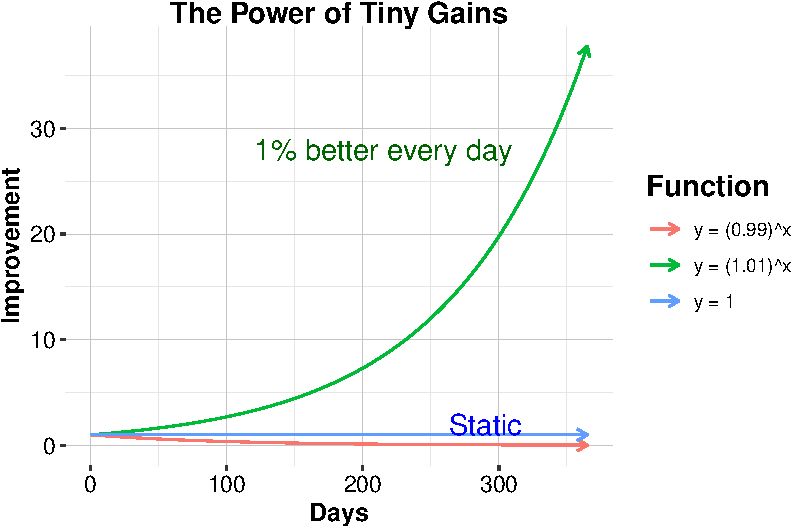
\includegraphics[width=0.7\linewidth,height=\textheight,keepaspectratio]{1-Intro-R_files/figure-pdf/fig-ch1-tiny-gains-1.pdf}

}

\caption{\label{fig-ch1-tiny-gains}The Power of Tiny Gains: A 1\%
improvement every day leads to exponential growth over time. This plot
was created entirely in R.}

\end{figure}%

Learning R is not about mastering everything at once. It is about making
steady progress, one concept at a time. With each small success (loading
a dataset, creating a plot, writing a function), you are building skills
that will support you throughout your data science journey. Be patient,
stay curious, and trust the process. Growth in programming, as in data,
is often exponential, just like the green line in
Figure~\ref{fig-ch1-tiny-gains}.

Now that you know what to expect and how to approach learning R, let us
begin by setting up your environment. In the next section, you will
install R and RStudio as your primary tools for writing and running R
code.

\section{How to Install R}\label{how-to-install-r}

Before you begin working with R, you need to install it on your
computer. R is freely available from the Comprehensive R Archive Network
(CRAN). Follow these steps:

\begin{enumerate}
\def\labelenumi{\arabic{enumi}.}
\item
  Visit the \href{https://cran.r-project.org}{CRAN website}.
\item
  Choose your operating system, Windows, macOS, or Linux.
\item
  Download the appropriate installer and follow the on-screen
  instructions to complete the installation.
\end{enumerate}

Once installed, you can use the R console directly. However, most users
prefer to work within an integrated development environment (IDE). In
the next section, we introduce RStudio, a popular and user-friendly
interface for writing and running R code.

\subsection*{Keeping R Up to Date}\label{keeping-r-up-to-date}
\addcontentsline{toc}{subsection}{Keeping R Up to Date}

R is updated regularly, with a major release each year, typically in
April, and several smaller updates in between. Staying current ensures
access to new features, performance improvements, and security patches.
It also helps maintain compatibility with the latest packages. That
said, frequent updates are not essential for beginners. If your current
setup works for your learning and analysis tasks, you can continue using
it without interruption.

When upgrading to a new major version, you may need to reinstall your R
packages. To simplify this process, you can save a list of your
installed packages using:

\begin{Shaded}
\begin{Highlighting}[]
\FunctionTok{installed.packages}\NormalTok{()[, }\DecValTok{1}\NormalTok{]}
\end{Highlighting}
\end{Shaded}

Alternatively, use a package manager like \textbf{pak} or \textbf{renv}
to snapshot and restore your setup. Although occasional updates may seem
inconvenient, they help keep your tools stable and your workflow
reliable in the long run.

\section{How to Install RStudio}\label{how-to-install-rstudio}

After installing the R software, it is helpful to use a dedicated set of
tools that make working with R more productive and enjoyable. RStudio is
a free and open-source integrated development environment (IDE) designed
specifically for R. It provides a clean interface, a powerful script
editor, and integrated tools for plotting, debugging, and package
management, all of which streamline the R programming experience.

\begin{quote}
\textbf{Note}: RStudio is an editor and does not include R itself. You
must install R before using RStudio.
\end{quote}

\subsection*{Installing RStudio}\label{installing-rstudio}
\addcontentsline{toc}{subsection}{Installing RStudio}

To install RStudio:

\begin{enumerate}
\def\labelenumi{\arabic{enumi}.}
\item
  Visit the \href{https://posit.co/download/rstudio-desktop}{RStudio
  website}.
\item
  Download the latest version of RStudio Desktop (the free, open-source
  edition) for your operating system, Windows, macOS, or Linux.
\item
  Run the installer and follow the on-screen instructions.
\item
  Launch RStudio---you are now ready to begin coding in R.
\end{enumerate}

RStudio is updated several times a year and typically notifies you when
a new version is available. Keeping it up to date is recommended so that
you can benefit from the latest features, stability improvements, and
bug fixes.

\subsection*{Exploring the RStudio
Interface}\label{exploring-the-rstudio-interface}
\addcontentsline{toc}{subsection}{Exploring the RStudio Interface}

When you open RStudio for the first time, you will see a layout similar
to Figure~\ref{fig-RStudio-window-1}. This integrated interface is
divided into four panels, each serving a specific purpose in your R
workflow.

\begin{figure}[H]

\centering{

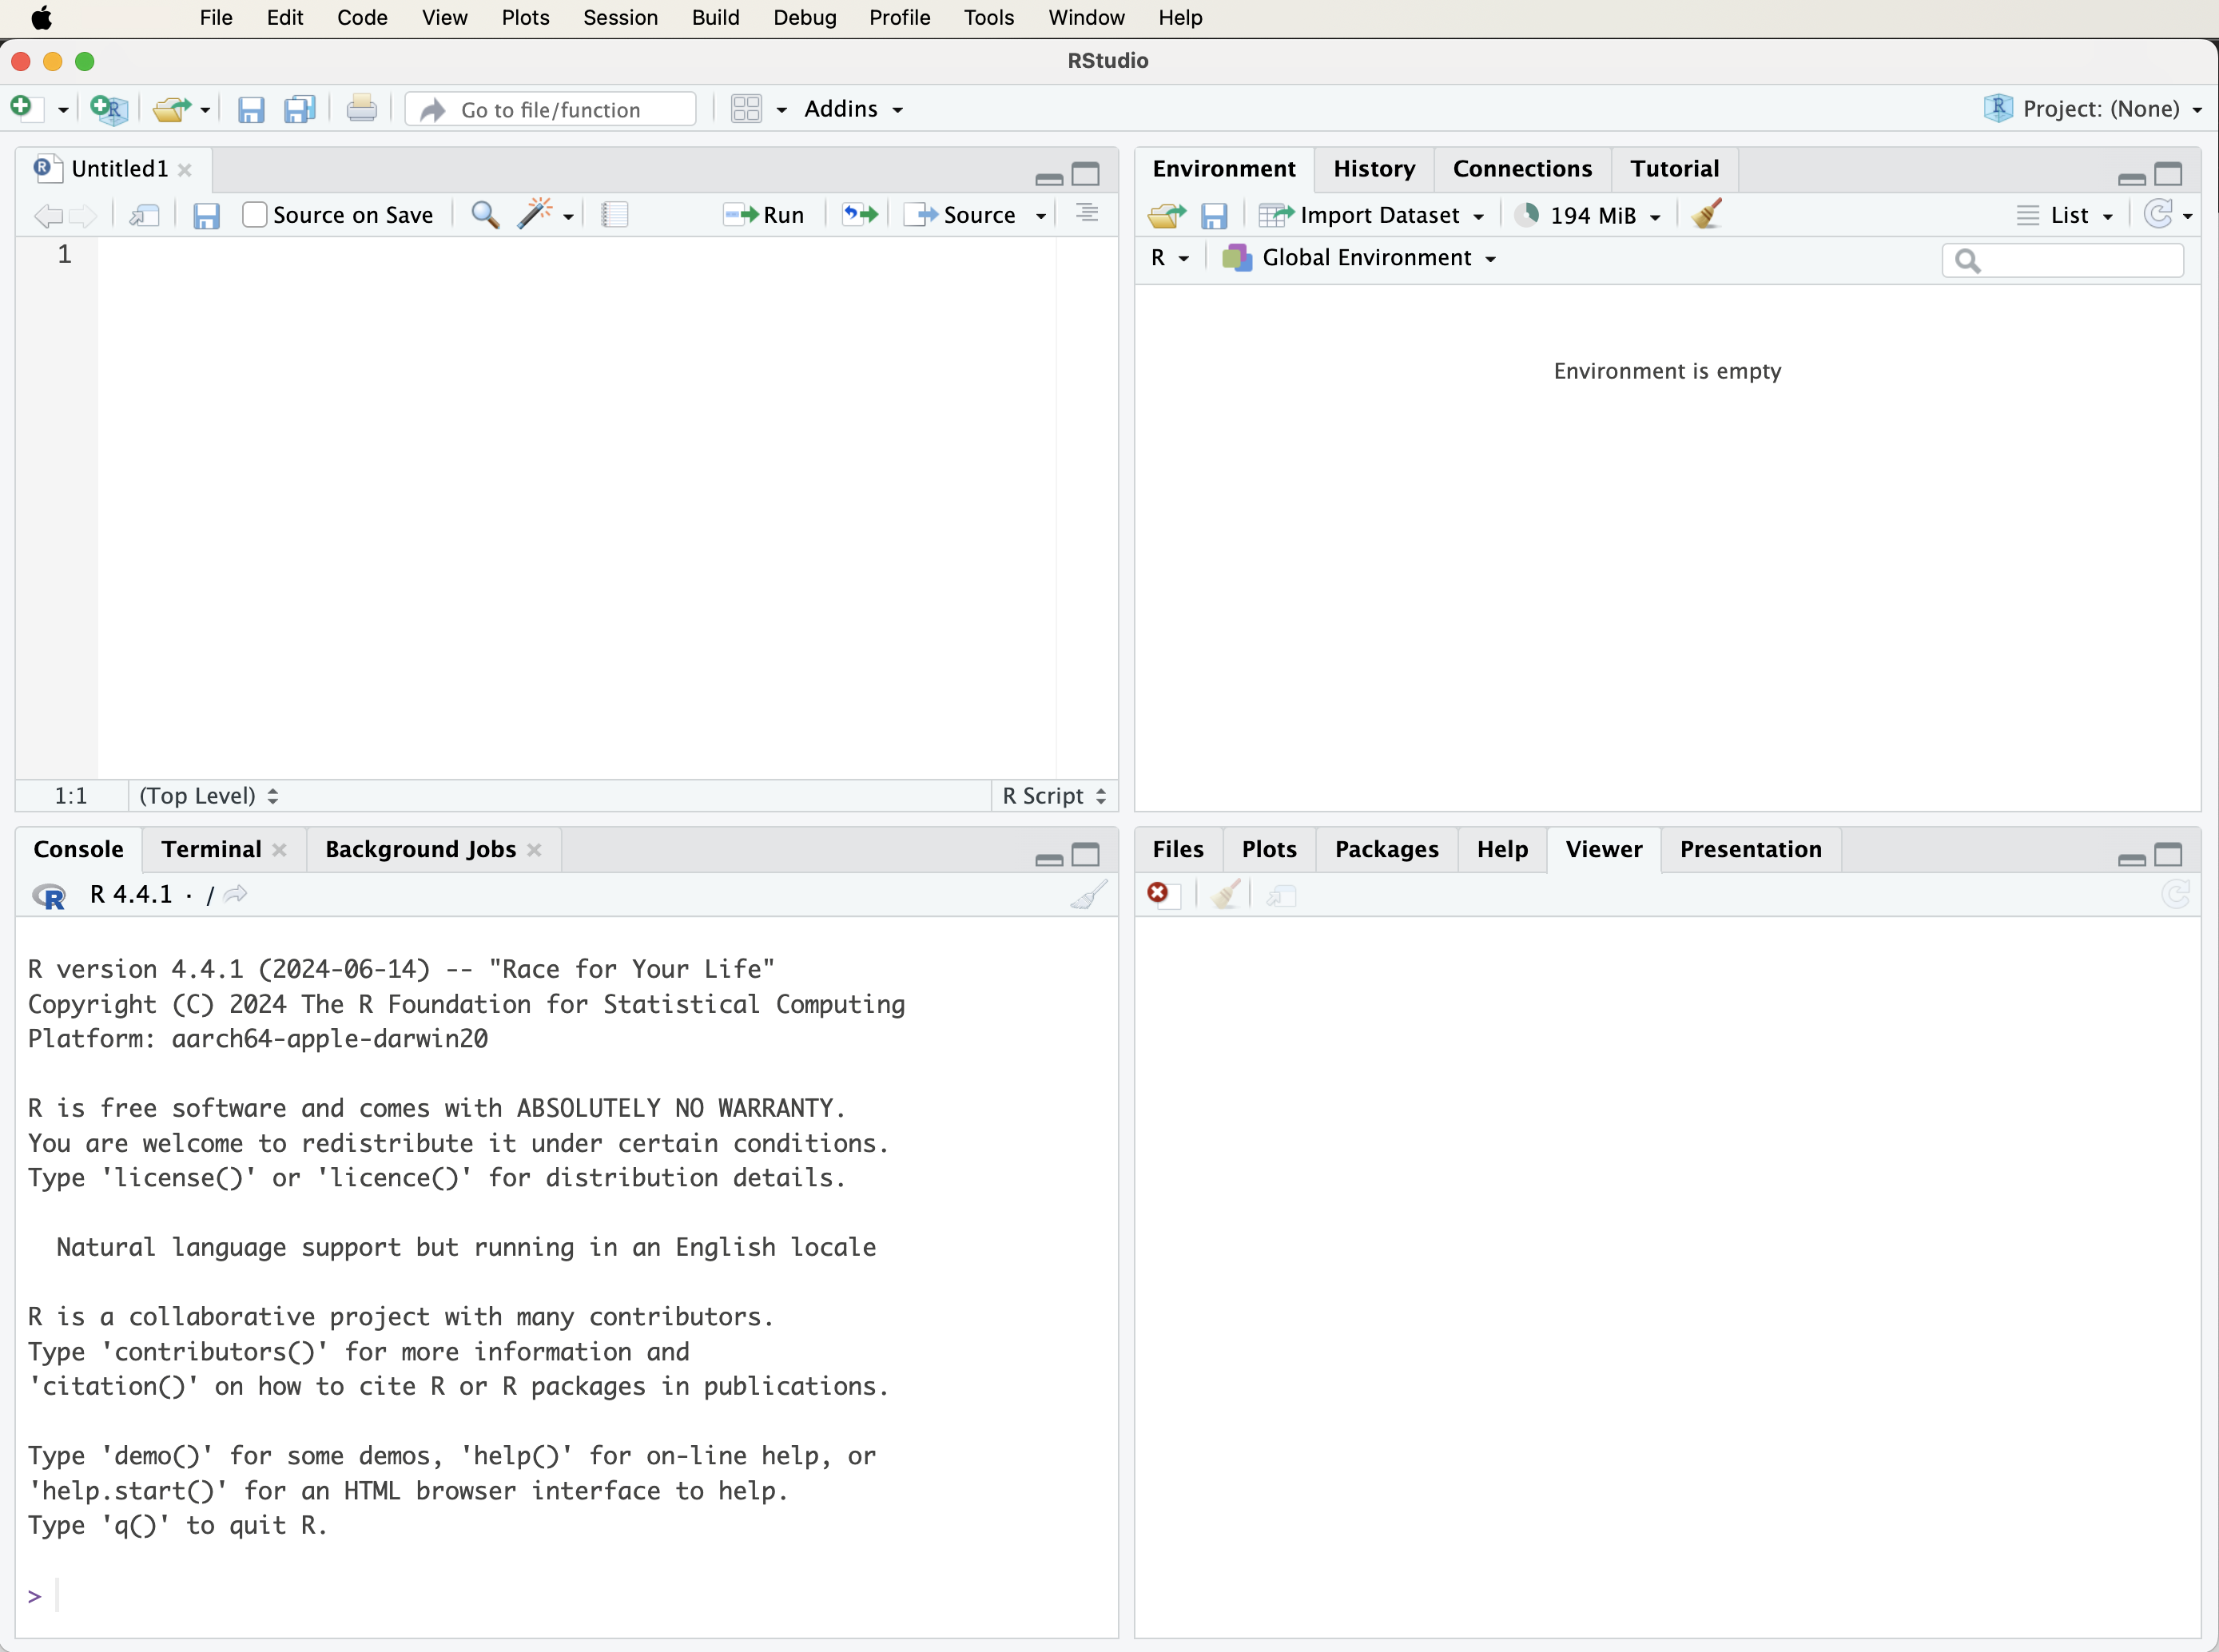
\includegraphics[width=0.65\linewidth,height=\textheight,keepaspectratio]{images/ch1_RStudio-window-1.png}

}

\caption{\label{fig-RStudio-window-1}The RStudio window when you first
launch the program.}

\end{figure}%

If only three panels are visible initially, select \emph{File
\textgreater{} New File \textgreater{} R Script} to open the script
editor. This panel enables you to write, edit, and save R code for
future use and reproducibility.

The four main panels are:

\begin{itemize}
\item
  \emph{Script Editor (top left)}: Write and edit R scripts.
\item
  \emph{Console (bottom left)}: Enter R commands and view their output.
\item
  \emph{Environment and History (top right)}: Inspect current variables
  and view previously executed commands.
\item
  \emph{Files, Plots, Packages, and Help (bottom right)}: Navigate
  files, visualize data, manage packages, and access documentation.
\end{itemize}

For now, focus on entering simple R commands into the console and
pressing \emph{Enter} to view the results. In later chapters, you will
gradually make use of each panel as your projects grow in complexity.

\subsection*{Customizing RStudio}\label{customizing-rstudio}
\addcontentsline{toc}{subsection}{Customizing RStudio}

As you begin working more extensively with R, it is worth taking a few
moments to tailor RStudio to your preferences. A well-organized and
comfortable environment can make your coding sessions more productive
and enjoyable.

To customize RStudio, go to:

\begin{quote}
\textbf{Tools \textgreater{} Global Options}
\end{quote}

From there, you can explore several settings to personalize your
workspace. For example:

\begin{itemize}
\item
  Under \emph{Appearance}, you can change the editor theme (e.g.,
  selecting \emph{Tomorrow Night 80} for dark mode) to reduce eye
  strain. You can also adjust font size, pane layout, and syntax
  highlighting to suit your style.
\item
  If installed, the \emph{Copilot} tab allows you to enable GitHub
  Copilot for AI-assisted code suggestions.
\end{itemize}

These small adjustments not only improve comfort and focus but also
support sustained engagement as you deepen your skills in R.

Now that your environment is set up, you might be wondering where to
turn when you get stuck or want to deepen your understanding. The next
section offers tips for getting help and continuing to learn.

\section{Getting Help and Learning
More}\label{getting-help-and-learning-more}

Learning R can be challenging at first; but you do not have to do it
alone. Today's learners have access to powerful support tools that can
dramatically accelerate the process. Among them, AI assistants like
ChatGPT offer a flexible, conversational way to learn faster, get
unstuck, and deepen your understanding.

With an AI assistant, you can ask questions in natural language and
receive immediate, context-aware guidance. Whether you are puzzled by an
error message, unsure how a function works, or looking for help writing
a block of code, tools like ChatGPT provide on-demand support. They can
walk you through code step-by-step, generate examples based on your
description, and explain unfamiliar concepts in clear, accessible
language. This makes them especially helpful during independent study or
when you need quick clarification without interrupting your workflow.

That said, AI tools are not the only resource. R includes robust
built-in documentation, type \texttt{?function\_name} or use
\texttt{help()} and \texttt{example()} in the console to access
function-specific help and sample usage. These features offer precise,
official information and remain a fundamental resource.

Online communities also play an important role. Sites such as
\href{https://stackoverflow.com/questions/tagged/r}{Stack Overflow} and
\href{https://community.rstudio.com}{RStudio Community} provide answers
to countless common problems. Searching these forums often reveals
solutions or helpful patterns. If you post a new question, remember to
include a clear explanation and a reproducible example.

In the end, the best way to learn R is to combine resources: practice
regularly, use AI tools to speed up your learning, consult the
documentation for accuracy, and turn to the community for collective
wisdom. With each small step, you will become more confident in your
ability to explore data, write code, and solve problems with R.

\section{Data Science and Machine Learning with
R}\label{data-science-and-machine-learning-with-r}

Imagine building a model that predicts hospital readmissions, optimizing
a marketing campaign, or uncovering fraud in financial transactions. All
of this is possible using code you understand and control. This book
teaches you how, using R, one of the most powerful tools in the data
scientist's toolkit.

This book introduces the core ideas and practical tools of data science
and machine learning, using R as the primary programming environment.
You will learn how to prepare data, build models, evaluate results, and
communicate insights. These skills are applied to real-world datasets
throughout the book.

R provides a solid foundation for statistical analysis and data
visualization. Its real strength, however, lies in its extensive
ecosystem of packages (modular libraries that extend the capabilities of
R for modern analytics). To support these capabilities, R relies on a
vast network of user-contributed packages developed by a global
community of researchers and practitioners. These packages are freely
available via the Comprehensive R Archive Network (CRAN).

While base R includes essential functions for data wrangling and basic
modeling, many advanced techniques, particularly in machine learning,
are implemented through contributed packages. A typical R package
contains functions for specific tasks, sample datasets for
experimentation, and documentation or vignettes to guide users.

Each machine learning method introduced in this book is paired with an
appropriate package implementation. For example, in Chapter
\ref{sec-ch11-tree-models}, we use \textbf{rpart} and
\textbf{randomForest} for decision trees and ensemble learning. In
Chapter \ref{sec-ch12-neural-networks}, we use \textbf{neuralnet} to
introduce the basics of neural network modeling. These tools are
introduced with clear examples and hands-on exercises to help you apply
them confidently.

To support the examples and exercises in this book, we developed the
\href{https://CRAN.R-project.org/package=liver}{\textbf{liver}} package.
It includes real-world datasets and utility functions specifically
designed for teaching data science with R. Several of these datasets are
listed in Table~\ref{tbl-data-table}. For example, in Chapter
\ref{sec-ch7-classification-knn}, we use one of these datasets to
demonstrate the k-nearest neighbors (kNN) classification algorithm using
functions from \textbf{liver}.

For those interested in going further, CRAN hosts thousands of
additional packages covering areas such as text mining, forecasting,
deep learning, and geospatial analysis. You can browse the full
repository at \url{https://CRAN.R-project.org}.

As you progress through this book, you will become not only proficient
in the R language but also fluent in using its rich ecosystem of
packages to tackle real data science challenges. With curiosity and
consistent practice, these tools will become part of your everyday
workflow.

\section{How to Install R Packages}\label{sec-install-packages}

Packages are central to working in R, they extend its core capabilities
and allow you to perform specialized tasks such as data wrangling,
modeling, and visualization. Many examples in this book use contributed
packages. You will be prompted to install them as needed, starting with
the \textbf{liver} package described below.

There are two common ways to install R packages: through RStudio's
graphical interface or by using the \texttt{install.packages()} function
in the R console.

To install a package using RStudio's interface:

\begin{enumerate}
\def\labelenumi{\arabic{enumi}.}
\item
  Click on the \emph{Tools} menu and select \emph{Install
  Packages\ldots{}}.
\item
  In the dialog box, enter the name of the package (or multiple packages
  separated by commas).
\item
  Make sure the \emph{Install dependencies} option is checked.
\item
  Click \emph{Install} to begin.
\end{enumerate}

See the screenshot in Figure \ref{fig-install-packages} for a visual
reference.

\begin{figure}[H]

\centering{

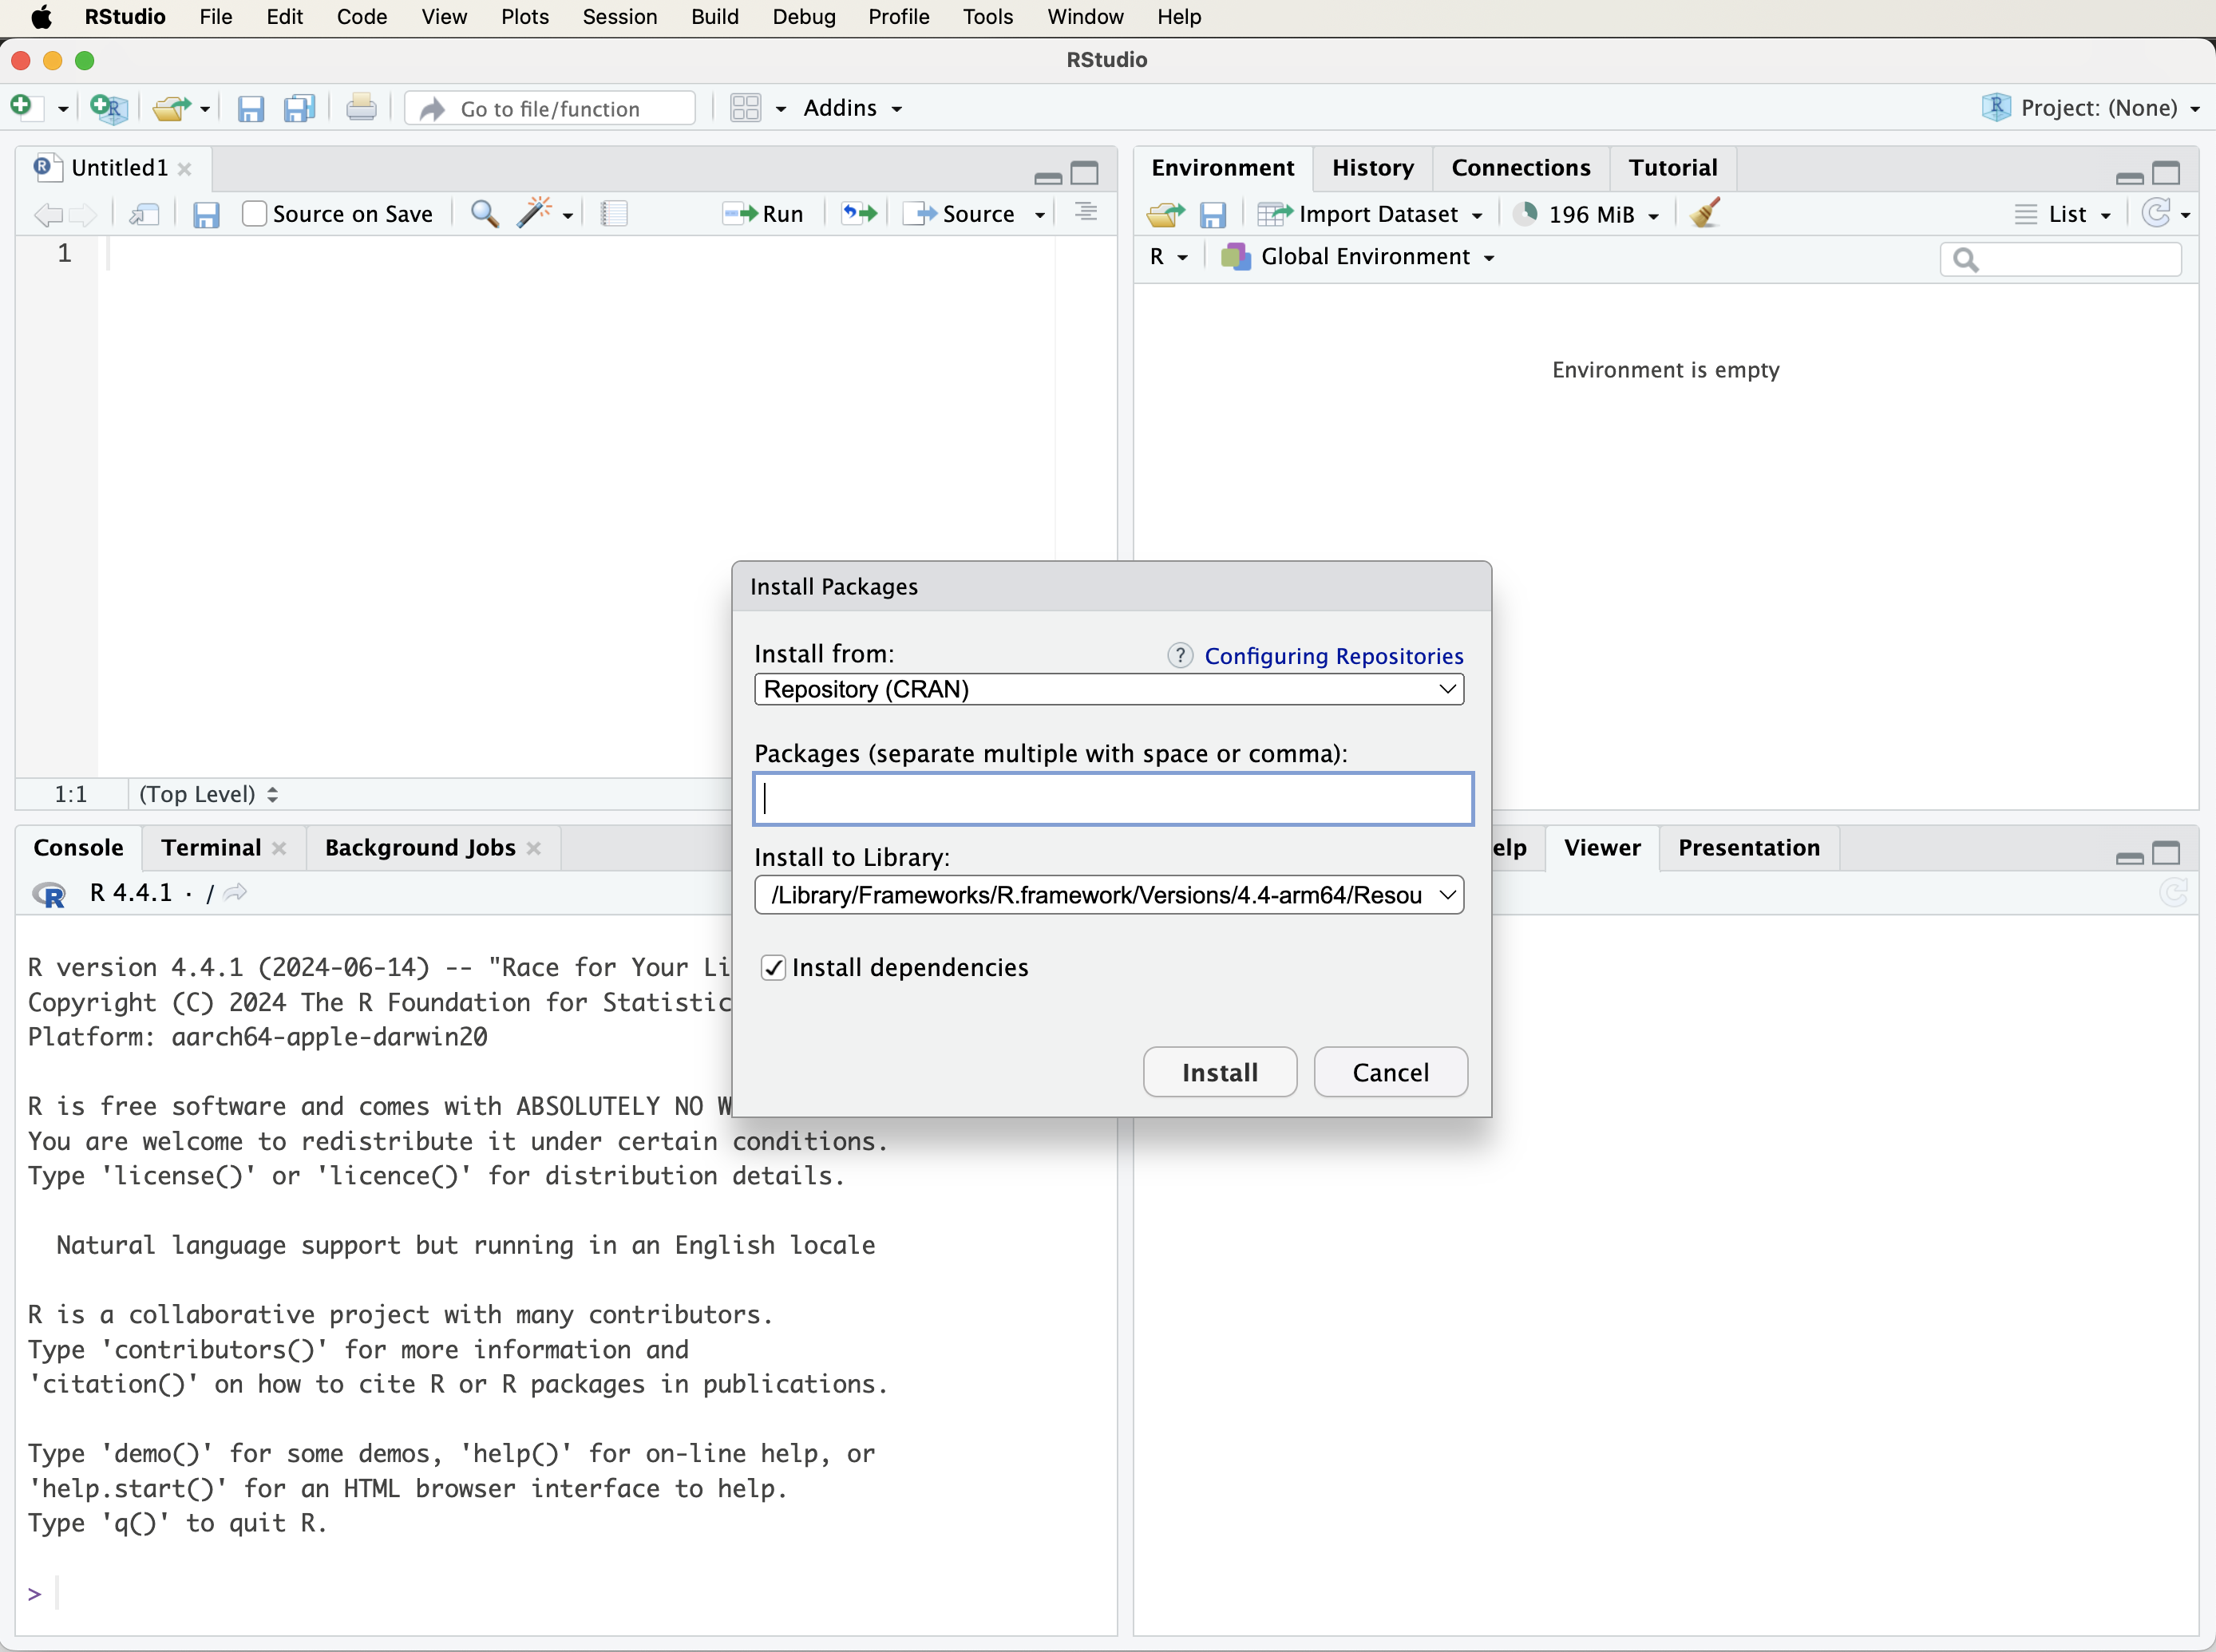
\includegraphics[width=0.65\linewidth,height=\textheight,keepaspectratio]{images/ch1_RStudio-window-install.png}

}

\caption{\label{fig-install-packages}Installing packages via the
graphical interface in RStudio.}

\end{figure}%

The second, and more flexible, method is to install packages directly
using the \texttt{install.packages()} function in the console. For
example, to install the \textbf{liver} package, which provides datasets
and functions used throughout this book, type:

\begin{Shaded}
\begin{Highlighting}[]
\FunctionTok{install.packages}\NormalTok{(}\StringTok{"liver"}\NormalTok{)}
\end{Highlighting}
\end{Shaded}

Press \emph{Enter} to execute the command. R will download the package
from \href{https://cran.r-project.org}{CRAN} and install it on your
system. The first time you install a package, you may be prompted to
select a CRAN mirror. Choose one geographically close to your location
for faster downloads.

If installation fails, check your internet connection or confirm that a
firewall is not blocking access to CRAN. The \texttt{install.packages()}
function can also be used to install packages from a local file or a
custom repository. To learn more, run:

\begin{Shaded}
\begin{Highlighting}[]
\NormalTok{?install.packages}
\end{Highlighting}
\end{Shaded}

Packages only need to be installed once. However, each time you open a
new R session, you must load the package using the \texttt{library()}
function. This will be explained in the next section.

\section{How to Load R Packages}\label{how-to-load-r-packages}

Once a package is installed, you need to load it into your R session
before you can use its functions and datasets. R does not automatically
load all installed packages; instead, it loads only those you explicitly
request. This helps keep your environment organized and efficient,
avoiding unnecessary memory use and potential conflicts between
packages.

To load a package, use the \texttt{library()} function. For example, to
load the \textbf{liver} package, enter:

\begin{Shaded}
\begin{Highlighting}[]
\FunctionTok{library}\NormalTok{(liver)}
\end{Highlighting}
\end{Shaded}

Press \emph{Enter} to execute the command. If you see an error such as
\texttt{"there\ is\ no\ package\ called\ \textquotesingle{}liver\textquotesingle{}"},
the package has not yet been installed. In that case, return to
Section~\ref{sec-install-packages} to review how to install packages
using either RStudio or the \texttt{install.packages()} function.

While installing a package makes it available on your system, loading it
with \texttt{library()} is necessary each time you start a new R
session. Only then will its functions and datasets be accessible in your
workspace.

As you progress through this book, you will use several other packages,
such as \textbf{ggplot2} for visualization and \textbf{randomForest} for
modeling, each introduced when needed. Occasionally, two or more
packages may contain functions with the same name. When this occurs, R
uses the version from the package most recently loaded.

To avoid ambiguity in such cases, use the \texttt{::} operator to
explicitly call a function from a specific package. For example, to use
the \texttt{partition()} function from the \textbf{liver} package (used
for splitting data into training and test sets), type:

\begin{Shaded}
\begin{Highlighting}[]
\NormalTok{liver}\SpecialCharTok{::}\FunctionTok{partition}\NormalTok{()}
\end{Highlighting}
\end{Shaded}

This approach helps ensure that your code remains clear and
reproducible, especially in larger projects where many packages are used
together.

\section{Running Your First R Code}\label{running-your-first-r-code}

One of the most empowering aspects of R is that it responds instantly to
your commands. This immediate feedback makes it ideal for
experimentation, learning, and developing intuition through trial and
error. Suppose you just made three online purchases and want to
calculate the total cost. In R, you can do that instantly:

\begin{Shaded}
\begin{Highlighting}[]
\FloatTok{49.23} \SpecialCharTok{+} \FloatTok{11.78} \SpecialCharTok{+} \FloatTok{38.99}
\NormalTok{   [}\DecValTok{1}\NormalTok{] }\DecValTok{100}
\end{Highlighting}
\end{Shaded}

Press \emph{Enter}, and R returns the result. You can also try
subtraction, multiplication, or division. Feel free to change the
numbers and experiment with different operations.

You can store the result in a variable for later use:

\begin{Shaded}
\begin{Highlighting}[]
\NormalTok{total }\OtherTok{\textless{}{-}} \FloatTok{49.23} \SpecialCharTok{+} \FloatTok{11.78} \SpecialCharTok{+} \FloatTok{38.99}
\end{Highlighting}
\end{Shaded}

The \texttt{\textless{}-} symbol is R's assignment operator: it stores
the value on the right under the name on the left. You can think of it
as labeling a box and placing something inside. While the \texttt{=}
operator (\texttt{total\ =\ ...}) also works, \texttt{\textless{}-} is
the preferred convention, especially inside function calls.

Although \texttt{\textless{}-} is the traditional assignment operator,
it is interchangeable with \texttt{=} in most situations. To keep the
examples in this book beginner-friendly and consistent with other
programming languages like Python, we will generally use \texttt{=} when
assigning values. Both styles are valid, and you may choose the one that
suits you best.

Once a value is stored, you can reuse it in future calculations. For
example, to add 21\% tax:

\begin{Shaded}
\begin{Highlighting}[]
\NormalTok{total }\SpecialCharTok{*} \FloatTok{1.21}
\NormalTok{   [}\DecValTok{1}\NormalTok{] }\DecValTok{121}
\end{Highlighting}
\end{Shaded}

R retrieves the value of \texttt{total} and performs the calculation.
Note that R is case-sensitive. This means \texttt{Total} and
\texttt{total} refer to different objects. Always pay attention to
capitalization when naming or calling variables and functions.

\begin{quote}
\emph{Try it yourself}: What is the standard sales tax or VAT rate in
your country? Replace \texttt{1.21} with your local multiplier (e.g.,
\texttt{1.07} for 7\% tax) and rerun the code. You could also assign the
rate to a variable like \texttt{tax\_rate\ \textless{}-\ 1.21} to make
your code more readable.
\end{quote}

As you begin writing more lines of code, it becomes helpful to add
comments that explain what each part is doing.

\subsection*{Using Comments to Explain Your
Code}\label{using-comments-to-explain-your-code}
\addcontentsline{toc}{subsection}{Using Comments to Explain Your Code}

Comments help explain what your code is doing, making it easier to
understand and maintain. In R, comments begin with a \texttt{\#} symbol.
Everything after \texttt{\#} on the same line is ignored when the code
runs.

Comments do not affect code execution but are essential for documenting
your reasoning, whether for teammates, future readers, or even yourself
after a few weeks. This is especially helpful in data science projects,
where analyses often involve multiple steps and assumptions.

Here is an example with multiple steps and explanatory comments:

\begin{Shaded}
\begin{Highlighting}[]
\CommentTok{\# Define prices of three items}
\NormalTok{prices }\OtherTok{\textless{}{-}} \FunctionTok{c}\NormalTok{(}\FloatTok{49.23}\NormalTok{, }\FloatTok{11.78}\NormalTok{, }\FloatTok{38.99}\NormalTok{)}

\CommentTok{\# Calculate the total cost}
\NormalTok{total }\OtherTok{\textless{}{-}} \FunctionTok{sum}\NormalTok{(prices)}

\CommentTok{\# Apply a 21\% tax}
\NormalTok{total }\SpecialCharTok{*} \FloatTok{1.21}
\NormalTok{   [}\DecValTok{1}\NormalTok{] }\DecValTok{121}
\end{Highlighting}
\end{Shaded}

Clear comments turn code into a readable narrative, which helps others
(and your future self) understand the logic behind your analysis.

\subsection*{How Functions Work in R}\label{how-functions-work-in-r}
\addcontentsline{toc}{subsection}{How Functions Work in R}

Functions are at the heart of R. They allow you to perform powerful
operations with just a line or two of code, whether you are calculating
a summary statistic, transforming a dataset, or creating a plot.
Learning how to use functions effectively is one of the most important
skills in your R journey.

A function typically takes one or more \emph{arguments} (inputs),
performs a task, and returns an \emph{output}. For example, the
\texttt{c()} function (short for ``combine'') creates a vector:

\begin{Shaded}
\begin{Highlighting}[]
\CommentTok{\# Define prices of three items}
\NormalTok{prices }\OtherTok{\textless{}{-}} \FunctionTok{c}\NormalTok{(}\FloatTok{49.23}\NormalTok{, }\FloatTok{11.78}\NormalTok{, }\FloatTok{38.99}\NormalTok{)}
\end{Highlighting}
\end{Shaded}

Once you have a vector, you can use another function to compute a
summary, such as the average:

\begin{Shaded}
\begin{Highlighting}[]
\FunctionTok{mean}\NormalTok{(prices)  }\CommentTok{\# Calculate the mean of prices}
\NormalTok{   [}\DecValTok{1}\NormalTok{] }\FloatTok{33.33333}
\end{Highlighting}
\end{Shaded}

The general structure of a function call in R looks like this:

\begin{Shaded}
\begin{Highlighting}[]
\FunctionTok{function\_name}\NormalTok{(argument1, argument2, ...)}
\end{Highlighting}
\end{Shaded}

Some functions require specific arguments, while others have optional
parameters with default values. To learn more about a function and its
arguments, type \texttt{?} followed by the function name:

\begin{Shaded}
\begin{Highlighting}[]
\NormalTok{?mean  }\CommentTok{\# or help(mean)}
\end{Highlighting}
\end{Shaded}

This opens the help documentation, including a description, argument
list, and example usage.

You will encounter many functions throughout this book, from basic
operations like \texttt{sum()} and \texttt{plot()} to specialized tools
for machine learning. Functions make your code concise, modular, and
expressive.

Throughout this book, you will use many built-in functions, often
combining them to perform complex tasks in just a few lines of code. For
now, focus on understanding how functions are structured and practicing
with common examples.

\section{Import Data into R}\label{sec-ch1-import-data}

Before you can explore, model, or visualize anything in R, you first
need to bring data into your session. Importing data is the starting
point for any analysis, and R supports a wide range of formats,
including text files, Excel spreadsheets, and datasets hosted on the
web. Depending on your needs and the file type, you can choose from
several efficient methods to load your data.

\subsection*{Importing Data with RStudio's Graphical
Interface}\label{importing-data-with-rstudios-graphical-interface}
\addcontentsline{toc}{subsection}{Importing Data with RStudio's
Graphical Interface}

For beginners, the easiest way to import data into R is through
RStudio's graphical interface. In the top-right \emph{Environment}
panel, click the \emph{Import Dataset} button (see Figure
\ref{fig-load-data}). A dialog box will appear, prompting you to choose
the type of file you want to load.

You can choose from several file types depending on your data source and
analysis goals. For example, text files such as CSV or tab-delimited
files can be loaded using the \emph{From Text (base)} option. Microsoft
Excel files can be imported via the \emph{From Excel} option, provided
the \textbf{readxl} package is installed. Additional formats may appear
depending on your installed packages and RStudio setup.

\begin{figure}[H]

\centering{

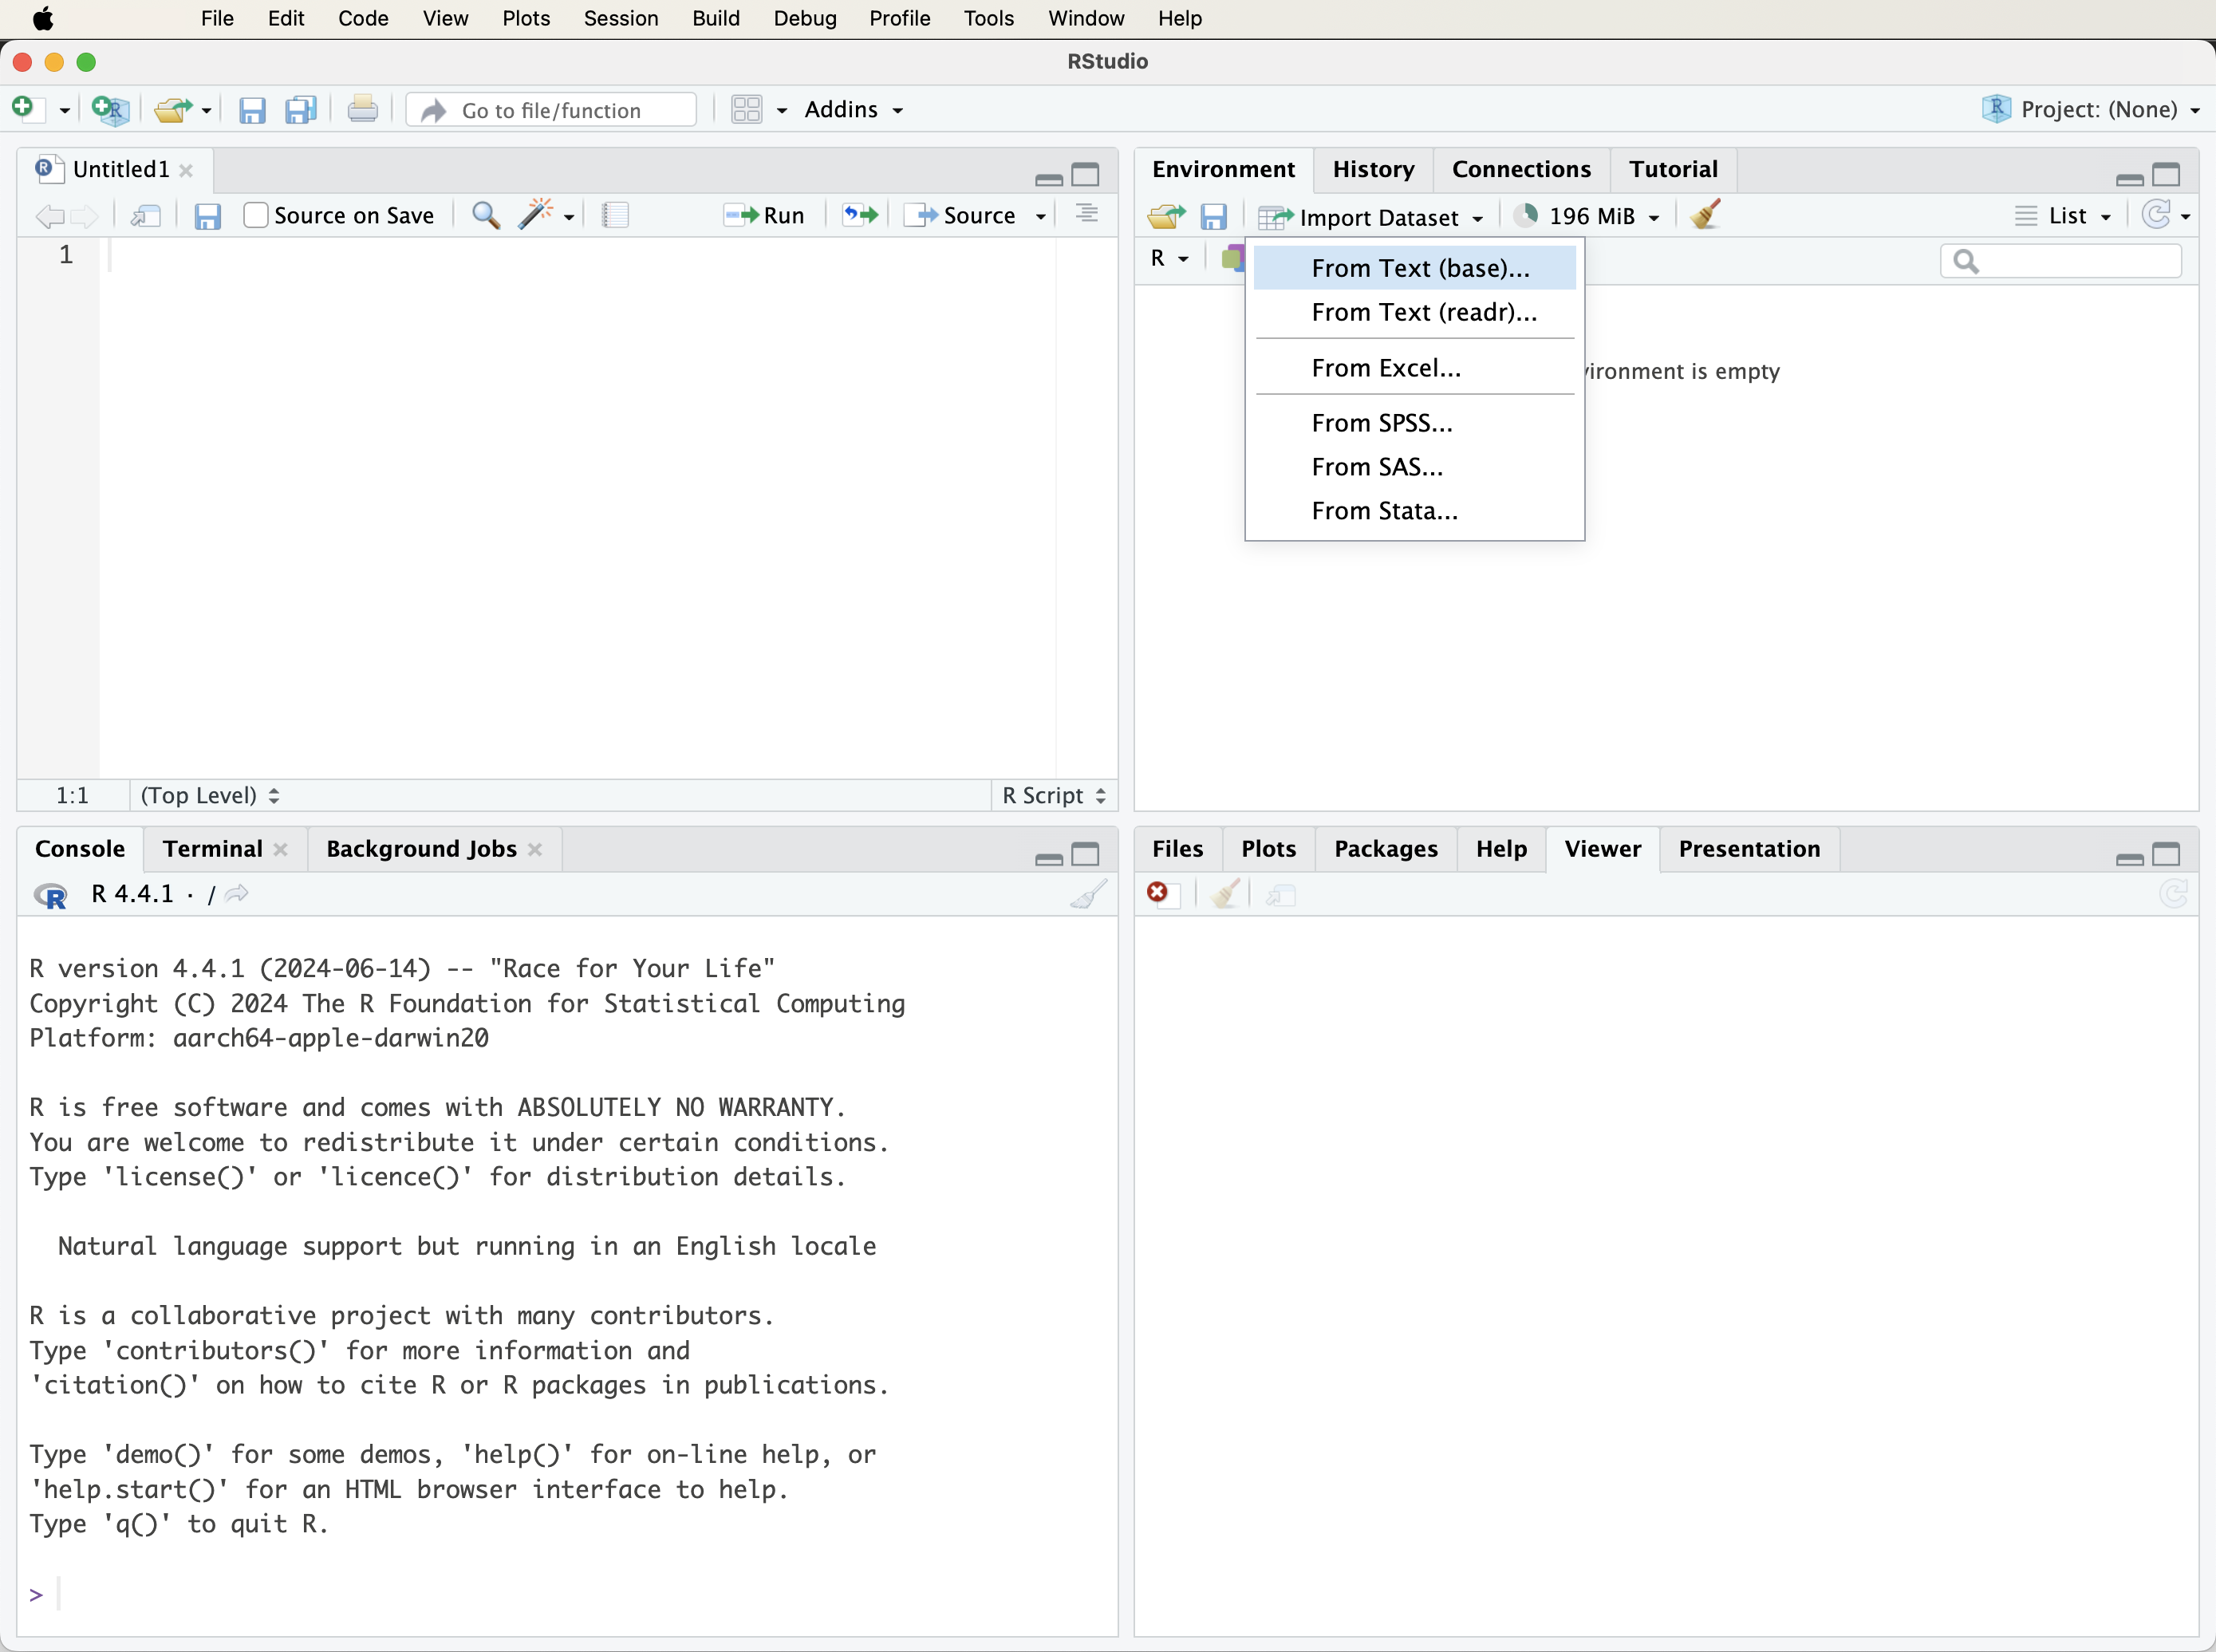
\includegraphics[width=0.65\linewidth,height=\textheight,keepaspectratio]{images/ch1_RStudio-window-data-1.png}

}

\caption{\label{fig-load-data}Using the `Import Dataset' tab in RStudio
to load data.}

\end{figure}%

After selecting a file, RStudio displays a preview window (Figure
\ref{fig-load-data-2}) where you can review and adjust options like
column names, separators, data types, and encoding. Once you confirm the
settings, click \emph{Import}. The dataset will be loaded into your
environment and appear in the \emph{Environment} panel, ready for
analysis.

\begin{figure}[H]

\centering{

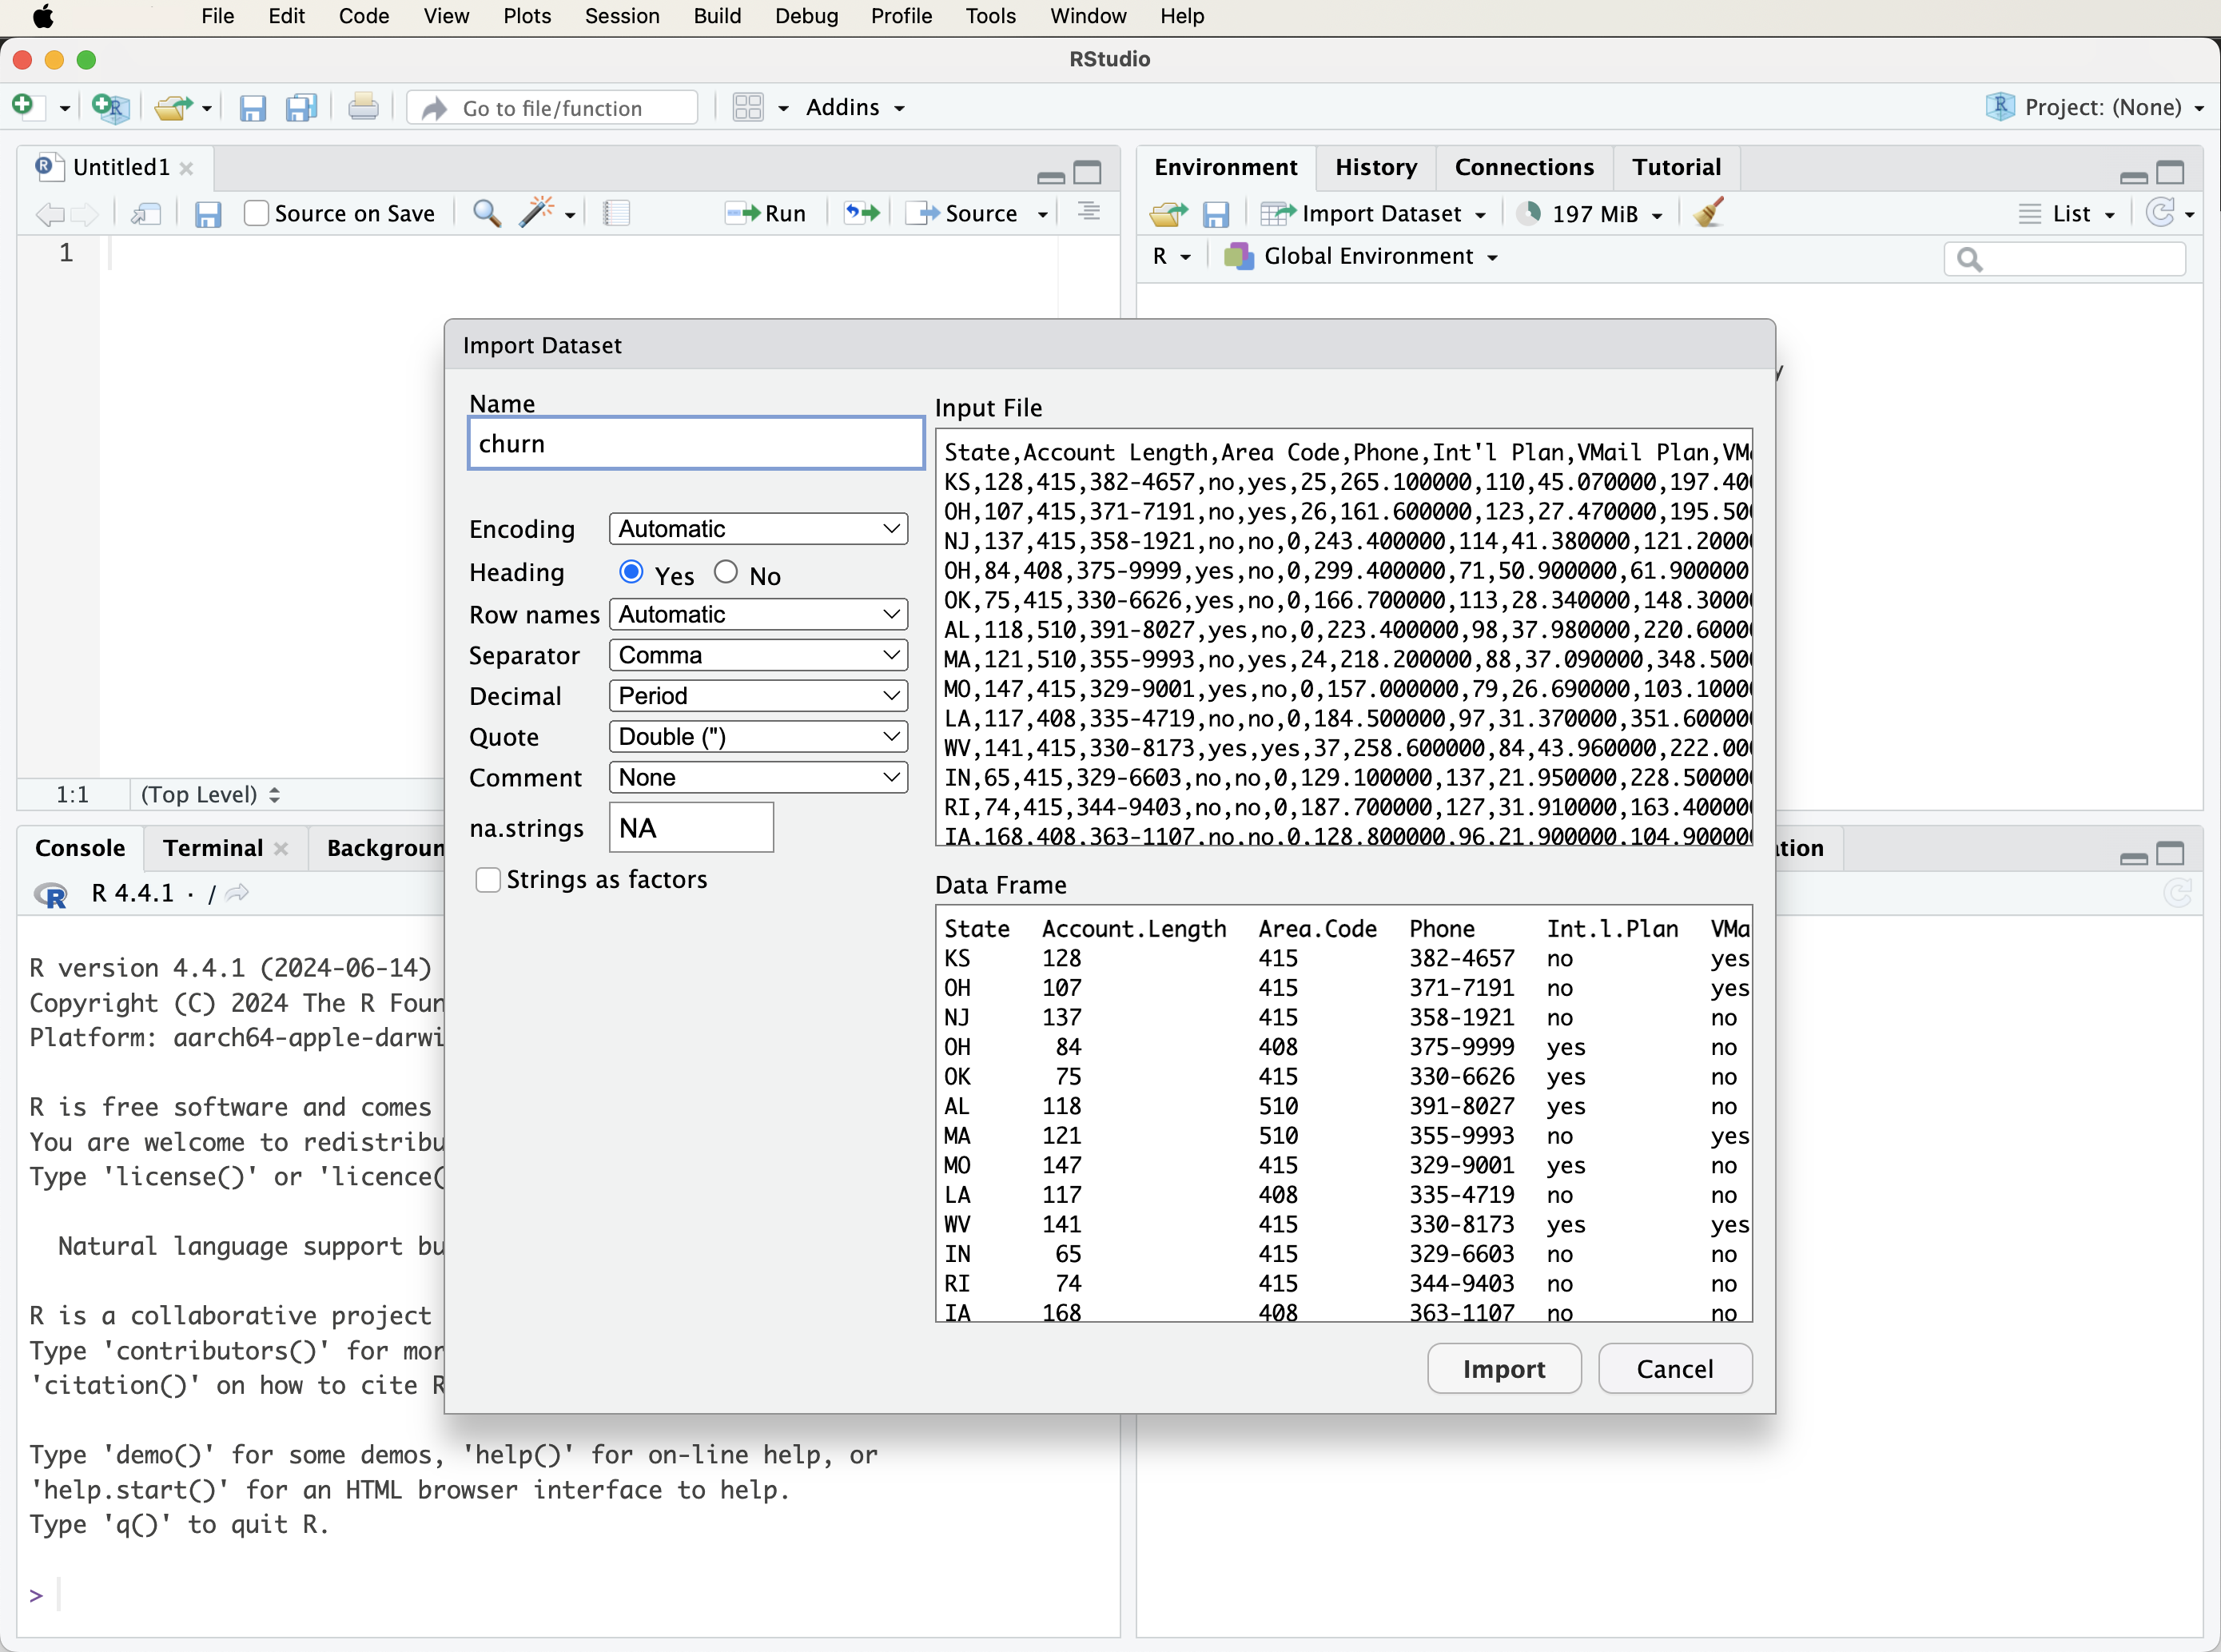
\includegraphics[width=0.65\linewidth,height=\textheight,keepaspectratio]{images/ch1_RStudio-window-data.png}

}

\caption{\label{fig-load-data-2}Adjusting import settings in RStudio
before loading the dataset.}

\end{figure}%

\subsection*{\texorpdfstring{Importing CSV Files with
\texttt{read.csv()}}{Importing CSV Files with read.csv()}}\label{importing-csv-files-with-read.csv}
\addcontentsline{toc}{subsection}{Importing CSV Files with
\texttt{read.csv()}}

If you prefer writing code, or want to make your analysis reproducible,
you can load CSV files using the \texttt{read.csv()} function from base
R. This is one of the most common ways to import data, especially for
scripting or automating workflows.

To load a CSV file from your computer, use:

\begin{Shaded}
\begin{Highlighting}[]
\NormalTok{data }\OtherTok{\textless{}{-}} \FunctionTok{read.csv}\NormalTok{(}\StringTok{"path/to/your/file.csv"}\NormalTok{)}
\end{Highlighting}
\end{Shaded}

Replace \texttt{"path/to/your/file.csv"} with the actual file path. If
your file does not include column names in the first row, set
\texttt{header\ =\ FALSE}:

\begin{Shaded}
\begin{Highlighting}[]
\NormalTok{data }\OtherTok{\textless{}{-}} \FunctionTok{read.csv}\NormalTok{(}\StringTok{"your\_file.csv"}\NormalTok{, }\AttributeTok{header =} \ConstantTok{FALSE}\NormalTok{)}
\end{Highlighting}
\end{Shaded}

If your dataset contains special characters, common in international
datasets or files saved from Excel, add the \texttt{fileEncoding}
argument to avoid import issues:

\begin{Shaded}
\begin{Highlighting}[]
\NormalTok{data }\OtherTok{\textless{}{-}} \FunctionTok{read.csv}\NormalTok{(}\StringTok{"your\_file.csv"}\NormalTok{, }\AttributeTok{fileEncoding =} \StringTok{"UTF{-}8{-}BOM"}\NormalTok{)}
\end{Highlighting}
\end{Shaded}

This ensures that R correctly interprets non-English characters and
symbols.

\subsection*{Setting the Working
Directory}\label{setting-the-working-directory}
\addcontentsline{toc}{subsection}{Setting the Working Directory}

The \emph{working directory} is the folder on your computer where R
looks for files to read, and where it saves any output by default. When
you import data, R will search this folder unless you give a full path
to the file.

To find out your current working directory, use:

\begin{Shaded}
\begin{Highlighting}[]
\FunctionTok{getwd}\NormalTok{()}
\end{Highlighting}
\end{Shaded}

To change it in code:

\begin{Shaded}
\begin{Highlighting}[]
\FunctionTok{setwd}\NormalTok{(}\StringTok{"\textasciitilde{}/Documents"}\NormalTok{)  }\CommentTok{\# Adjust this path to match your system}
\end{Highlighting}
\end{Shaded}

You can also change it through the RStudio menu:

\begin{quote}
\emph{Session \textgreater{} Set Working Directory \textgreater{} Choose
Directory\ldots{}}
\end{quote}

Setting the working directory properly can save time and reduce errors
when loading or saving files. If you're getting ``file not found''
errors, checking the working directory is a good first step.

\subsection*{Importing Data Using Dialogs and
URLs}\label{importing-data-using-dialogs-and-urls}
\addcontentsline{toc}{subsection}{Importing Data Using Dialogs and URLs}

Sometimes you may not want to hard-code a file path or prefer to work
with data hosted online. R offers flexible methods that make your
workflow more portable and user-friendly.

To allow users to choose a file interactively, use the
\texttt{file.choose()} function with \texttt{read.csv()}. This opens a
file selection dialog box:

\begin{Shaded}
\begin{Highlighting}[]
\NormalTok{data }\OtherTok{\textless{}{-}} \FunctionTok{read.csv}\NormalTok{(}\AttributeTok{file =} \FunctionTok{file.choose}\NormalTok{())}
\end{Highlighting}
\end{Shaded}

This is particularly handy when sharing code across different systems,
where file locations may vary.

You can also import data directly from a URL by passing it to
\texttt{read.csv()}:

\begin{Shaded}
\begin{Highlighting}[]
\NormalTok{data }\OtherTok{\textless{}{-}} \FunctionTok{read.csv}\NormalTok{(}\StringTok{"https://example.com/data.csv"}\NormalTok{)}
\end{Highlighting}
\end{Shaded}

This method is ideal for accessing public datasets from governments,
research institutions, or data repositories. It ensures your code stays
reproducible and eliminates the need for manual downloads.

Whether you are automating tasks or collaborating across platforms,
these import options make it easier to load data without setup friction.

\subsection*{\texorpdfstring{Importing Excel Files with
\texttt{read\_excel()}}{Importing Excel Files with read\_excel()}}\label{importing-excel-files-with-read_excel}
\addcontentsline{toc}{subsection}{Importing Excel Files with
\texttt{read\_excel()}}

Excel is one of the most common formats for storing data in business,
education, and research. To import \texttt{.xlsx} or \texttt{.xls} files
into R, use the \texttt{read\_excel()} function from the \textbf{readxl}
package, a lightweight, user-friendly tool in the tidyverse ecosystem.

If you have not installed the package yet, follow the guidance in
Section~\ref{sec-install-packages}, or use this command:

\begin{Shaded}
\begin{Highlighting}[]
\FunctionTok{install.packages}\NormalTok{(}\StringTok{"readxl"}\NormalTok{)}
\end{Highlighting}
\end{Shaded}

Then load the package and import your Excel file:

\begin{Shaded}
\begin{Highlighting}[]
\FunctionTok{library}\NormalTok{(readxl)}
\NormalTok{data }\OtherTok{\textless{}{-}} \FunctionTok{read\_excel}\NormalTok{(}\StringTok{"path/to/your/file.xlsx"}\NormalTok{)}
\end{Highlighting}
\end{Shaded}

Replace \texttt{"path/to/your/file.xlsx"} with the actual file path.

Unlike \texttt{read.csv()}, \texttt{read\_excel()} supports multiple
sheets in a single workbook. To import a specific sheet, use the
\texttt{sheet} argument:

\begin{Shaded}
\begin{Highlighting}[]
\NormalTok{data }\OtherTok{\textless{}{-}} \FunctionTok{read\_excel}\NormalTok{(}\StringTok{"path/to/your/file.xlsx"}\NormalTok{, }\AttributeTok{sheet =} \DecValTok{2}\NormalTok{)}
\end{Highlighting}
\end{Shaded}

This is especially useful when Excel files contain separate tables
across different tabs. If your file includes merged cells, multi-row
headers, or other formatting quirks, it is best to clean it in Excel
first, or handle it programmatically in R after import.

\subsection*{Loading Data from R
Packages}\label{loading-data-from-r-packages}
\addcontentsline{toc}{subsection}{Loading Data from R Packages}

In addition to reading external files, R also provides access to
datasets that come bundled with packages. These datasets are immediately
usable and are ideal for practice, examples, and case studies.

In this book, we use the \textbf{liver} package, developed specifically
for teaching purposes, which includes several real-world datasets. One
of the main datasets is \texttt{churn}, which contains information on
customer behavior in a telecommunications context. If you have not
installed the package yet, follow the guidance in
Section~\ref{sec-install-packages}.

To load the dataset into your environment, run:

\begin{Shaded}
\begin{Highlighting}[]
\FunctionTok{library}\NormalTok{(liver) }\CommentTok{\# To load the liver package}

\FunctionTok{data}\NormalTok{(churn)    }\CommentTok{\# To load the churn dataset}
\end{Highlighting}
\end{Shaded}

Once loaded, \texttt{churn} will appear in your Environment tab and can
be used like any other data frame. This dataset, along with others
listed in Table \ref{tbl-data-table}, will appear throughout the book in
examples related to modeling, evaluation, and visualization. In Chapter
\ref{sec-ch4-EDA}, you will perform exploratory data analysis (EDA) on
\texttt{churn} to uncover patterns and prepare it for modeling.

\begin{quote}
\emph{Try it yourself}: After loading \texttt{churn}, use
\texttt{head(churn)} or \texttt{str(churn)} to explore its structure and
variables.
\end{quote}

Using datasets embedded in packages like \textbf{liver} ensures that
your analysis is reproducible and portable across systems, since the
data can be loaded consistently in any R session.

\section{Why Data Types Matter in R}\label{why-data-types-matter-in-r}

In R, every object (whether a number, string, or logical value) has a
data type. These types play a critical role in how R stores, processes,
and interprets data. Recognizing the correct type is essential for
ensuring that computations behave as expected and that analyses yield
valid results.

Here are the most common data types in R:

\emph{Numeric}: Real numbers such as \texttt{3.14} or \texttt{-5.67}.
Used for continuous values such as weight, temperature, or income; they
support arithmetic operations.

\emph{Integer}: Whole numbers like \texttt{1}, \texttt{42}, or
\texttt{-6}. Integers are useful for counting, indexing rows, or
representing categories with numeric codes.

\emph{Character}: Text values such as \texttt{"Data\ Science"} or
\texttt{"Azizam"}. Character data is used for names, descriptions,
labels, and other textual content.

\emph{Logical}: Boolean values, \texttt{TRUE} or \texttt{FALSE}. Logical
values are used for comparisons, filtering, and conditional statements.

\emph{Factor}: Categorical variables with a defined set of levels (e.g.,
\texttt{"Yes"} and \texttt{"No"}). Factors are essential in modeling and
grouped visualizations, where the variable should behave as a category
rather than text.

To check the type of a variable, use the \texttt{class()} function:

\begin{Shaded}
\begin{Highlighting}[]
\FunctionTok{class}\NormalTok{(prices)}
\NormalTok{   [}\DecValTok{1}\NormalTok{] }\StringTok{"numeric"}
\end{Highlighting}
\end{Shaded}

This tells you the broad data type R assigns to the variable. To inspect
how R stores it internally, use \texttt{typeof()}. To explore complex
structures like data frames, use \texttt{str()}:

\begin{Shaded}
\begin{Highlighting}[]
\FunctionTok{typeof}\NormalTok{(prices)}
\NormalTok{   [}\DecValTok{1}\NormalTok{] }\StringTok{"double"}
\FunctionTok{str}\NormalTok{(prices)}
\NormalTok{    num [}\DecValTok{1}\SpecialCharTok{:}\DecValTok{3}\NormalTok{] }\FloatTok{49.2} \FloatTok{11.8} \DecValTok{39}
\end{Highlighting}
\end{Shaded}

Why does this matter? Treating a numeric variable as character, or vice
versa, can cause functions to return incorrect results or warnings. For
example:

\begin{Shaded}
\begin{Highlighting}[]
\NormalTok{income }\OtherTok{\textless{}{-}} \FunctionTok{c}\NormalTok{(}\StringTok{"42000"}\NormalTok{, }\StringTok{"28000"}\NormalTok{, }\StringTok{"60000"}\NormalTok{)  }\CommentTok{\# Stored as character}

\FunctionTok{mean}\NormalTok{(income)   }\CommentTok{\# This will return NA with a warning}
\NormalTok{   [}\DecValTok{1}\NormalTok{] }\ConstantTok{NA}
\end{Highlighting}
\end{Shaded}

In this case, R interprets income as text, not numbers. You can fix the
issue by converting the character vector to numeric:

\begin{Shaded}
\begin{Highlighting}[]
\NormalTok{income }\OtherTok{\textless{}{-}} \FunctionTok{as.numeric}\NormalTok{(income)}

\FunctionTok{mean}\NormalTok{(income)}
\NormalTok{   [}\DecValTok{1}\NormalTok{] }\FloatTok{43333.33}
\end{Highlighting}
\end{Shaded}

Later chapters, such as Exploratory Data Analysis (Chapter
\ref{sec-ch4-EDA}) and Statistical Inference (Chapter
\ref{sec-ch5-statistics}), will show you how to apply tools specific to
each variable type, whether for summarizing values, visualizing
distributions, or building models.

\begin{quote}
\emph{Try it yourself}: Load the \texttt{churn} dataset from the
\textbf{liver} package (see Section~\ref{sec-ch1-import-data}). Then use
\texttt{str(churn)} to inspect its structure. Which variables are
numeric, character, or factors? Try using \texttt{class()} and
\texttt{typeof()} on a few columns to explore how R understands them.
\end{quote}

\section{Data Structures in R}\label{data-structures-in-r}

In R, data structures define how information is organized, stored, and
manipulated. Choosing the right structure is essential for effective
analysis, whether you are summarizing data, creating visualizations, or
building predictive models. For example, storing customer names and
purchases calls for a different structure than tracking the results of a
simulation.

Data structures are different from data types: data types describe
\emph{what} a value is (e.g., a number or a string), while data
structures describe \emph{how} values are arranged and grouped (e.g., in
a table, matrix, or list).

The most commonly used structures in R include vectors, matrices, data
frames, lists, and arrays. Each is suited to particular tasks and
workflows. Figure \ref{fig-R-objects} provides a visual overview of
these core structures.

\begin{figure}[H]

\centering{

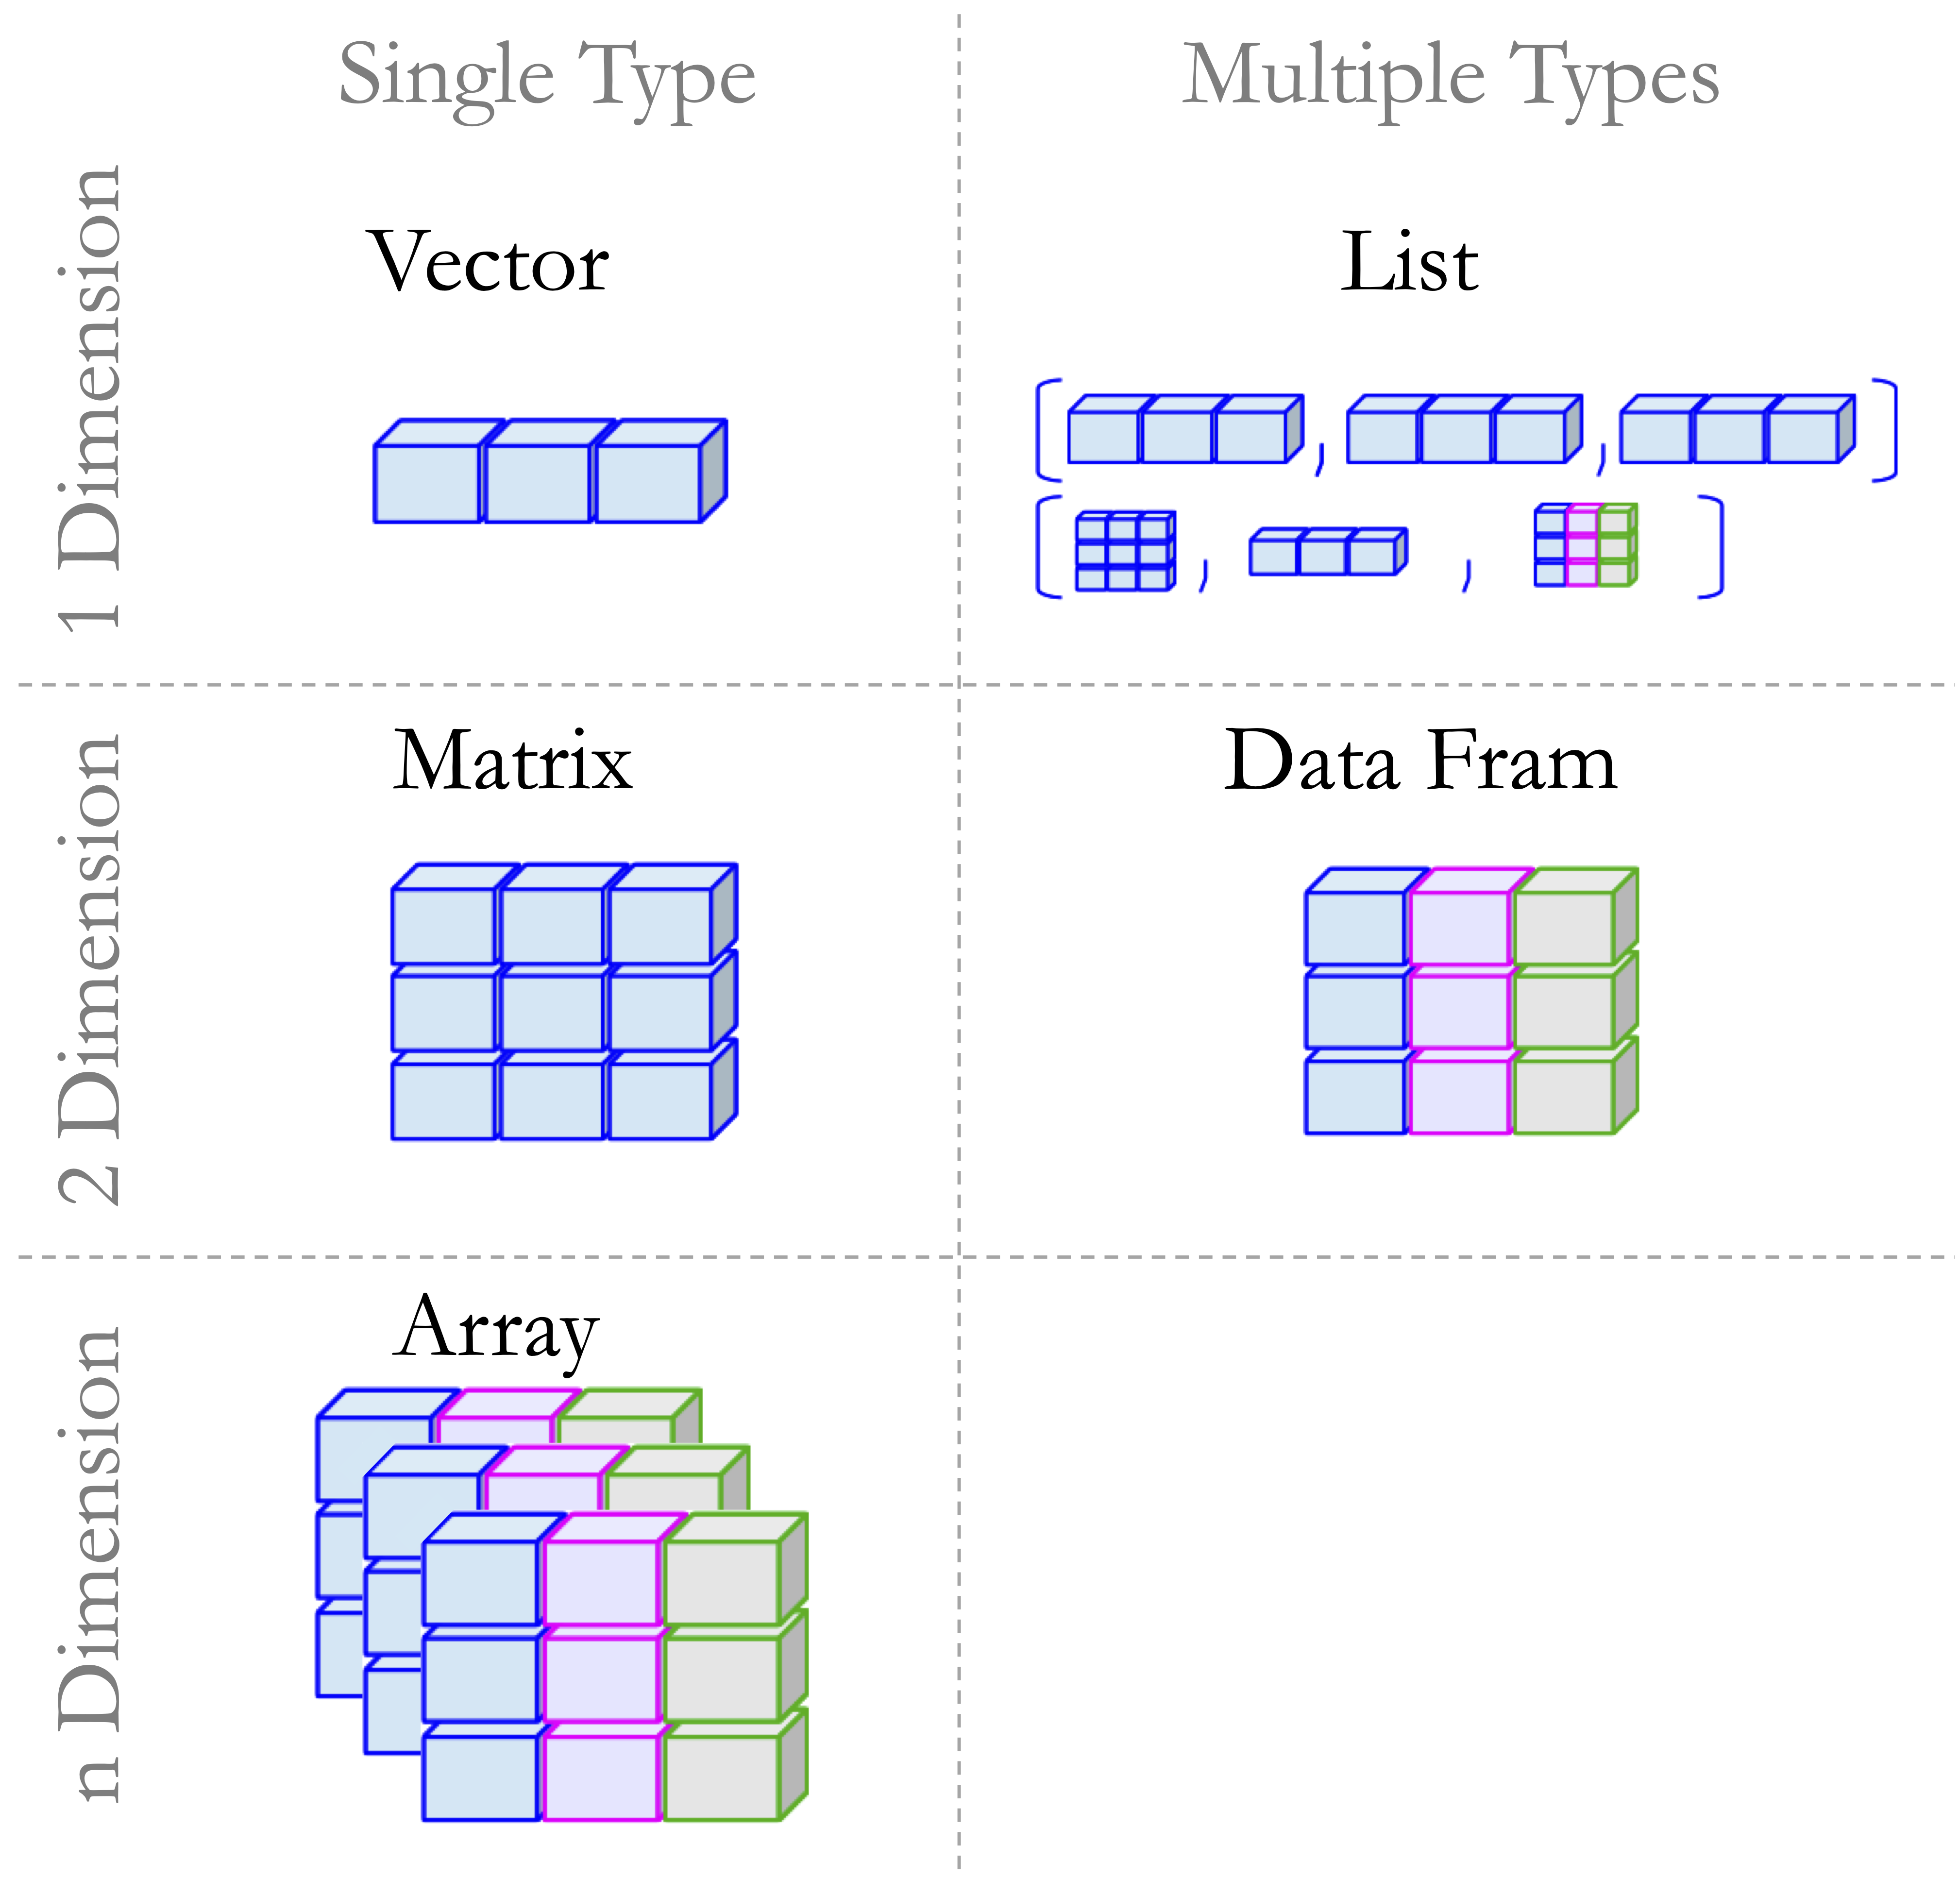
\includegraphics[width=0.55\linewidth,height=\textheight,keepaspectratio]{images/ch1_R-objects.png}

}

\caption{\label{fig-R-objects}A visual guide to five common data
structures in R, organized by dimensionality (1D, 2D, nD) and type
uniformity (single vs.~multiple types).}

\end{figure}%

In this section, we explore how to create and work with the four most
commonly used data structures in R: vectors, matrices, data frames, and
lists, each illustrated with practical examples showing when and how to
use them.

\subsection*{Vectors in R}\label{vectors-in-r}
\addcontentsline{toc}{subsection}{Vectors in R}

A \emph{vector} is the most fundamental data structure in R. It
represents a one-dimensional sequence of elements, all of the \emph{same
type}; for example, all numbers, all text strings, or all logical values
(\texttt{TRUE} or \texttt{FALSE}). Vectors form the foundation of many
other R structures, including matrices and data frames.

You can create a vector using the \texttt{c()} function (short for
\emph{combine}), which concatenates individual elements into a single
sequence:

\begin{Shaded}
\begin{Highlighting}[]
\CommentTok{\# Create a numeric vector representing prices of three items}
\NormalTok{prices }\OtherTok{\textless{}{-}} \FunctionTok{c}\NormalTok{(}\FloatTok{49.23}\NormalTok{, }\FloatTok{11.78}\NormalTok{, }\FloatTok{38.99}\NormalTok{)}

\CommentTok{\# Print the vector}
\NormalTok{prices}
\NormalTok{   [}\DecValTok{1}\NormalTok{] }\FloatTok{49.23} \FloatTok{11.78} \FloatTok{38.99}

\CommentTok{\# Check if \textasciigrave{}prices\textasciigrave{} is a vector}
\FunctionTok{is.vector}\NormalTok{(prices)}
\NormalTok{   [}\DecValTok{1}\NormalTok{] }\ConstantTok{TRUE}

\CommentTok{\# Get the number of elements in the vector}
\FunctionTok{length}\NormalTok{(prices)}
\NormalTok{   [}\DecValTok{1}\NormalTok{] }\DecValTok{3}
\end{Highlighting}
\end{Shaded}

In this example, \texttt{prices} is a numeric vector containing three
elements. The \texttt{is.vector()} function checks whether the object is
a vector, and \texttt{length(prices)} tells you how many elements it
contains.

\begin{quote}
\emph{Note:} All elements in a vector must be of the same type. If you
mix types (for example, numbers and characters), R will coerce them to a
common type, usually character, which can sometimes lead to unintended
consequences.
\end{quote}

\subsection*{Matrices in R}\label{matrices-in-r}
\addcontentsline{toc}{subsection}{Matrices in R}

A \emph{matrix} is a two-dimensional data structure in R where all
elements must be of the same type (numeric, character, or logical).
Matrices are commonly used in mathematics, statistics, and machine
learning for operations involving rows and columns.

To create a matrix, use the \texttt{matrix()} function. Here is a simple
example:

\begin{Shaded}
\begin{Highlighting}[]
\CommentTok{\# Create a matrix with 2 rows and 3 columns, filled row by row}
\NormalTok{my\_matrix }\OtherTok{\textless{}{-}} \FunctionTok{matrix}\NormalTok{(}\FunctionTok{c}\NormalTok{(}\DecValTok{1}\NormalTok{, }\DecValTok{2}\NormalTok{, }\DecValTok{3}\NormalTok{, }\DecValTok{4}\NormalTok{, }\DecValTok{5}\NormalTok{, }\DecValTok{6}\NormalTok{), }\AttributeTok{nrow =} \DecValTok{2}\NormalTok{, }\AttributeTok{ncol =} \DecValTok{3}\NormalTok{, }\AttributeTok{byrow =} \ConstantTok{TRUE}\NormalTok{)}

\CommentTok{\# Display the matrix}
\NormalTok{my\_matrix}
\NormalTok{        [,}\DecValTok{1}\NormalTok{] [,}\DecValTok{2}\NormalTok{] [,}\DecValTok{3}\NormalTok{]}
\NormalTok{   [}\DecValTok{1}\NormalTok{,]    }\DecValTok{1}    \DecValTok{2}    \DecValTok{3}
\NormalTok{   [}\DecValTok{2}\NormalTok{,]    }\DecValTok{4}    \DecValTok{5}    \DecValTok{6}

\CommentTok{\# Check if it\textquotesingle{}s a matrix}
\FunctionTok{is.matrix}\NormalTok{(my\_matrix)}
\NormalTok{   [}\DecValTok{1}\NormalTok{] }\ConstantTok{TRUE}

\CommentTok{\# Check its dimensions (rows, columns)}
\FunctionTok{dim}\NormalTok{(my\_matrix)}
\NormalTok{   [}\DecValTok{1}\NormalTok{] }\DecValTok{2} \DecValTok{3}
\end{Highlighting}
\end{Shaded}

This creates a \(2 \times 3\) matrix filled \emph{row by row} using the
numbers 1 through 6. If you leave out the \texttt{byrow\ =\ TRUE}
argument (or set it to \texttt{FALSE}), R fills the matrix \emph{column
by column}, which is the default behavior.

Matrices are useful in a wide range of numerical operations, such as
matrix multiplication, linear transformations, or storing pairwise
distances. They form the backbone of many machine learning algorithms
and statistical models. Most core computations in neural networks,
support vector machines, and linear regression rely on matrix operations
behind the scenes.

You can access specific elements using row and column indices:

\begin{Shaded}
\begin{Highlighting}[]
\CommentTok{\# Access the element in row 1, column 2}
\NormalTok{my\_matrix[}\DecValTok{1}\NormalTok{, }\DecValTok{2}\NormalTok{]}
\NormalTok{   [}\DecValTok{1}\NormalTok{] }\DecValTok{2}
\end{Highlighting}
\end{Shaded}

This retrieves the value in the first row and second column. You can
also label rows and columns using \texttt{rownames()} and
\texttt{colnames()} for easier interpretation in analysis.

\begin{quote}
\emph{Try it yourself}: Create a \(3 \times 3\) matrix with your own
numbers. Can you retrieve the value in the third row and first column?
\end{quote}

\subsection*{Data Frames in R}\label{data-frames-in-r}
\addcontentsline{toc}{subsection}{Data Frames in R}

A \emph{data frame} is one of the most important and commonly used data
structures in R. It organizes data in a two-dimensional layout, rows and
columns, where each column can store a different data type: numeric,
character, logical, or factor. This flexibility makes data frames ideal
for tabular data, similar to what you might encounter in a spreadsheet
or database.

In this book, nearly all datasets, whether built-in or imported from
external files, are stored and analyzed as data frames. Understanding
how to work with data frames is essential for following the examples and
building your own analyses.

You can create a data frame by combining vectors of equal length using
the \texttt{data.frame()} function:

\begin{Shaded}
\begin{Highlighting}[]
\CommentTok{\# Create vectors for student data}
\NormalTok{student\_id }\OtherTok{\textless{}{-}} \FunctionTok{c}\NormalTok{(}\DecValTok{101}\NormalTok{, }\DecValTok{102}\NormalTok{, }\DecValTok{103}\NormalTok{, }\DecValTok{104}\NormalTok{)}
\NormalTok{name       }\OtherTok{\textless{}{-}} \FunctionTok{c}\NormalTok{(}\StringTok{"Emma"}\NormalTok{, }\StringTok{"Bob"}\NormalTok{, }\StringTok{"Alice"}\NormalTok{, }\StringTok{"Noah"}\NormalTok{)}
\NormalTok{age        }\OtherTok{\textless{}{-}} \FunctionTok{c}\NormalTok{(}\DecValTok{20}\NormalTok{, }\DecValTok{21}\NormalTok{, }\DecValTok{19}\NormalTok{, }\DecValTok{22}\NormalTok{)}
\NormalTok{grade      }\OtherTok{\textless{}{-}} \FunctionTok{c}\NormalTok{(}\StringTok{"A"}\NormalTok{, }\StringTok{"B"}\NormalTok{, }\StringTok{"A"}\NormalTok{, }\StringTok{"C"}\NormalTok{)}

\CommentTok{\# Combine vectors into a data frame}
\NormalTok{students\_df }\OtherTok{\textless{}{-}} \FunctionTok{data.frame}\NormalTok{(student\_id, name, age, grade)}

\CommentTok{\# Display the data frame}
\NormalTok{students\_df}
\NormalTok{     student\_id  name age grade}
   \DecValTok{1}        \DecValTok{101}\NormalTok{  Emma  }\DecValTok{20}\NormalTok{     A}
   \DecValTok{2}        \DecValTok{102}\NormalTok{   Bob  }\DecValTok{21}\NormalTok{     B}
   \DecValTok{3}        \DecValTok{103}\NormalTok{ Alice  }\DecValTok{19}\NormalTok{     A}
   \DecValTok{4}        \DecValTok{104}\NormalTok{  Noah  }\DecValTok{22}\NormalTok{     C}
\end{Highlighting}
\end{Shaded}

This creates a data frame named \texttt{students\_df} with four columns.
Each row represents a student, and each column holds a different type of
information. To confirm the object's structure, use:

\begin{Shaded}
\begin{Highlighting}[]
\FunctionTok{class}\NormalTok{(students\_df)}
\NormalTok{   [}\DecValTok{1}\NormalTok{] }\StringTok{"data.frame"}
\FunctionTok{is.data.frame}\NormalTok{(students\_df)}
\NormalTok{   [}\DecValTok{1}\NormalTok{] }\ConstantTok{TRUE}
\end{Highlighting}
\end{Shaded}

To explore the contents of a data frame, try:

\begin{Shaded}
\begin{Highlighting}[]
\FunctionTok{head}\NormalTok{(students\_df)     }\CommentTok{\# View the first few rows}
\NormalTok{     student\_id  name age grade}
   \DecValTok{1}        \DecValTok{101}\NormalTok{  Emma  }\DecValTok{20}\NormalTok{     A}
   \DecValTok{2}        \DecValTok{102}\NormalTok{   Bob  }\DecValTok{21}\NormalTok{     B}
   \DecValTok{3}        \DecValTok{103}\NormalTok{ Alice  }\DecValTok{19}\NormalTok{     A}
   \DecValTok{4}        \DecValTok{104}\NormalTok{  Noah  }\DecValTok{22}\NormalTok{     C}
\FunctionTok{str}\NormalTok{(students\_df)      }\CommentTok{\# View column types and structure}
   \StringTok{\textquotesingle{}data.frame\textquotesingle{}}\SpecialCharTok{:}    \DecValTok{4}\NormalTok{ obs. of  }\DecValTok{4}\NormalTok{ variables}\SpecialCharTok{:}
    \ErrorTok{$}\NormalTok{ student\_id}\SpecialCharTok{:}\NormalTok{ num  }\DecValTok{101} \DecValTok{102} \DecValTok{103} \DecValTok{104}
    \SpecialCharTok{$}\NormalTok{ name      }\SpecialCharTok{:}\NormalTok{ chr  }\StringTok{"Emma"} \StringTok{"Bob"} \StringTok{"Alice"} \StringTok{"Noah"}
    \SpecialCharTok{$}\NormalTok{ age       }\SpecialCharTok{:}\NormalTok{ num  }\DecValTok{20} \DecValTok{21} \DecValTok{19} \DecValTok{22}
    \SpecialCharTok{$}\NormalTok{ grade     }\SpecialCharTok{:}\NormalTok{ chr  }\StringTok{"A"} \StringTok{"B"} \StringTok{"A"} \StringTok{"C"}
\FunctionTok{summary}\NormalTok{(students\_df)  }\CommentTok{\# Summary statistics by column}
\NormalTok{      student\_id        name                age           grade          }
\NormalTok{    Min.   }\SpecialCharTok{:}\FloatTok{101.0}\NormalTok{   Length}\SpecialCharTok{:}\DecValTok{4}\NormalTok{           Min.   }\SpecialCharTok{:}\FloatTok{19.00}\NormalTok{   Length}\SpecialCharTok{:}\DecValTok{4}          
    \DecValTok{1}\NormalTok{st Qu.}\SpecialCharTok{:}\FloatTok{101.8}\NormalTok{   Class }\SpecialCharTok{:}\NormalTok{character   }\DecValTok{1}\NormalTok{st Qu.}\SpecialCharTok{:}\FloatTok{19.75}\NormalTok{   Class }\SpecialCharTok{:}\NormalTok{character  }
\NormalTok{    Median }\SpecialCharTok{:}\FloatTok{102.5}\NormalTok{   Mode  }\SpecialCharTok{:}\NormalTok{character   Median }\SpecialCharTok{:}\FloatTok{20.50}\NormalTok{   Mode  }\SpecialCharTok{:}\NormalTok{character  }
\NormalTok{    Mean   }\SpecialCharTok{:}\FloatTok{102.5}\NormalTok{                      Mean   }\SpecialCharTok{:}\FloatTok{20.50}                     
    \DecValTok{3}\NormalTok{rd Qu.}\SpecialCharTok{:}\FloatTok{103.2}                      \DecValTok{3}\NormalTok{rd Qu.}\SpecialCharTok{:}\FloatTok{21.25}                     
\NormalTok{    Max.   }\SpecialCharTok{:}\FloatTok{104.0}\NormalTok{                      Max.   }\SpecialCharTok{:}\FloatTok{22.00}
\end{Highlighting}
\end{Shaded}

\subsubsection*{Accessing and Modifying
Columns}\label{accessing-and-modifying-columns}
\addcontentsline{toc}{subsubsection}{Accessing and Modifying Columns}

You can extract a specific column from a data frame using the
\texttt{\$} operator or square brackets:

\begin{Shaded}
\begin{Highlighting}[]
\CommentTok{\# Access the \textquotesingle{}age\textquotesingle{} column}
\NormalTok{students\_df}\SpecialCharTok{$}\NormalTok{age}
\NormalTok{   [}\DecValTok{1}\NormalTok{] }\DecValTok{20} \DecValTok{21} \DecValTok{19} \DecValTok{22}
\end{Highlighting}
\end{Shaded}

You can also use \texttt{students\_df{[}{[}"age"{]}{]}} or
\texttt{students\_df{[},\ "age"{]}}, try each one to see how they work.

To modify a column, for example, to add 1 to each age:

\begin{Shaded}
\begin{Highlighting}[]
\NormalTok{students\_df}\SpecialCharTok{$}\NormalTok{age }\OtherTok{\textless{}{-}}\NormalTok{ students\_df}\SpecialCharTok{$}\NormalTok{age }\SpecialCharTok{+} \DecValTok{1}
\end{Highlighting}
\end{Shaded}

You can also add a new column:

\begin{Shaded}
\begin{Highlighting}[]
\CommentTok{\# Add a logical column based on age}
\NormalTok{students\_df}\SpecialCharTok{$}\NormalTok{is\_adult }\OtherTok{\textless{}{-}}\NormalTok{ students\_df}\SpecialCharTok{$}\NormalTok{age }\SpecialCharTok{\textgreater{}=} \DecValTok{21}
\end{Highlighting}
\end{Shaded}

This creates a new column called \texttt{is\_adult} with \texttt{TRUE}
or \texttt{FALSE} values.

Data frames are especially useful in real-world analysis, where datasets
often mix numerical and categorical variables. For example, in this
book, we frequently use the \emph{churn} dataset from the \textbf{liver}
package:

\begin{Shaded}
\begin{Highlighting}[]
\FunctionTok{library}\NormalTok{(liver)   }\CommentTok{\# Load the liver package}
\FunctionTok{data}\NormalTok{(churn)      }\CommentTok{\# Load the churn dataset}

\CommentTok{\# Explore the structure of the data}
\FunctionTok{str}\NormalTok{(churn)}
   \StringTok{\textquotesingle{}data.frame\textquotesingle{}}\SpecialCharTok{:}    \DecValTok{5000}\NormalTok{ obs. of  }\DecValTok{20}\NormalTok{ variables}\SpecialCharTok{:}
    \ErrorTok{$}\NormalTok{ state         }\SpecialCharTok{:}\NormalTok{ Factor w}\SpecialCharTok{/} \DecValTok{51}\NormalTok{ levels }\StringTok{"AK"}\NormalTok{,}\StringTok{"AL"}\NormalTok{,}\StringTok{"AR"}\NormalTok{,..}\SpecialCharTok{:} \DecValTok{17} \DecValTok{36} \DecValTok{32} \DecValTok{36} \DecValTok{37} \DecValTok{2} \DecValTok{20} \DecValTok{25} \DecValTok{19} \DecValTok{50}\NormalTok{ ...}
    \SpecialCharTok{$}\NormalTok{ area.code     }\SpecialCharTok{:}\NormalTok{ Factor w}\SpecialCharTok{/} \DecValTok{3}\NormalTok{ levels }\StringTok{"area\_code\_408"}\NormalTok{,..}\SpecialCharTok{:} \DecValTok{2} \DecValTok{2} \DecValTok{2} \DecValTok{1} \DecValTok{2} \DecValTok{3} \DecValTok{3} \DecValTok{2} \DecValTok{1} \DecValTok{2}\NormalTok{ ...}
    \SpecialCharTok{$}\NormalTok{ account.length}\SpecialCharTok{:}\NormalTok{ int  }\DecValTok{128} \DecValTok{107} \DecValTok{137} \DecValTok{84} \DecValTok{75} \DecValTok{118} \DecValTok{121} \DecValTok{147} \DecValTok{117} \DecValTok{141}\NormalTok{ ...}
    \SpecialCharTok{$}\NormalTok{ voice.plan    }\SpecialCharTok{:}\NormalTok{ Factor w}\SpecialCharTok{/} \DecValTok{2}\NormalTok{ levels }\StringTok{"yes"}\NormalTok{,}\StringTok{"no"}\SpecialCharTok{:} \DecValTok{1} \DecValTok{1} \DecValTok{2} \DecValTok{2} \DecValTok{2} \DecValTok{2} \DecValTok{1} \DecValTok{2} \DecValTok{2} \DecValTok{1}\NormalTok{ ...}
    \SpecialCharTok{$}\NormalTok{ voice.messages}\SpecialCharTok{:}\NormalTok{ int  }\DecValTok{25} \DecValTok{26} \DecValTok{0} \DecValTok{0} \DecValTok{0} \DecValTok{0} \DecValTok{24} \DecValTok{0} \DecValTok{0} \DecValTok{37}\NormalTok{ ...}
    \SpecialCharTok{$}\NormalTok{ intl.plan     }\SpecialCharTok{:}\NormalTok{ Factor w}\SpecialCharTok{/} \DecValTok{2}\NormalTok{ levels }\StringTok{"yes"}\NormalTok{,}\StringTok{"no"}\SpecialCharTok{:} \DecValTok{2} \DecValTok{2} \DecValTok{2} \DecValTok{1} \DecValTok{1} \DecValTok{1} \DecValTok{2} \DecValTok{1} \DecValTok{2} \DecValTok{1}\NormalTok{ ...}
    \SpecialCharTok{$}\NormalTok{ intl.mins     }\SpecialCharTok{:}\NormalTok{ num  }\DecValTok{10} \FloatTok{13.7} \FloatTok{12.2} \FloatTok{6.6} \FloatTok{10.1} \FloatTok{6.3} \FloatTok{7.5} \FloatTok{7.1} \FloatTok{8.7} \FloatTok{11.2}\NormalTok{ ...}
    \SpecialCharTok{$}\NormalTok{ intl.calls    }\SpecialCharTok{:}\NormalTok{ int  }\DecValTok{3} \DecValTok{3} \DecValTok{5} \DecValTok{7} \DecValTok{3} \DecValTok{6} \DecValTok{7} \DecValTok{6} \DecValTok{4} \DecValTok{5}\NormalTok{ ...}
    \SpecialCharTok{$}\NormalTok{ intl.charge   }\SpecialCharTok{:}\NormalTok{ num  }\FloatTok{2.7} \FloatTok{3.7} \FloatTok{3.29} \FloatTok{1.78} \FloatTok{2.73} \FloatTok{1.7} \FloatTok{2.03} \FloatTok{1.92} \FloatTok{2.35} \FloatTok{3.02}\NormalTok{ ...}
    \SpecialCharTok{$}\NormalTok{ day.mins      }\SpecialCharTok{:}\NormalTok{ num  }\DecValTok{265} \DecValTok{162} \DecValTok{243} \DecValTok{299} \DecValTok{167}\NormalTok{ ...}
    \SpecialCharTok{$}\NormalTok{ day.calls     }\SpecialCharTok{:}\NormalTok{ int  }\DecValTok{110} \DecValTok{123} \DecValTok{114} \DecValTok{71} \DecValTok{113} \DecValTok{98} \DecValTok{88} \DecValTok{79} \DecValTok{97} \DecValTok{84}\NormalTok{ ...}
    \SpecialCharTok{$}\NormalTok{ day.charge    }\SpecialCharTok{:}\NormalTok{ num  }\FloatTok{45.1} \FloatTok{27.5} \FloatTok{41.4} \FloatTok{50.9} \FloatTok{28.3}\NormalTok{ ...}
    \SpecialCharTok{$}\NormalTok{ eve.mins      }\SpecialCharTok{:}\NormalTok{ num  }\FloatTok{197.4} \FloatTok{195.5} \FloatTok{121.2} \FloatTok{61.9} \FloatTok{148.3}\NormalTok{ ...}
    \SpecialCharTok{$}\NormalTok{ eve.calls     }\SpecialCharTok{:}\NormalTok{ int  }\DecValTok{99} \DecValTok{103} \DecValTok{110} \DecValTok{88} \DecValTok{122} \DecValTok{101} \DecValTok{108} \DecValTok{94} \DecValTok{80} \DecValTok{111}\NormalTok{ ...}
    \SpecialCharTok{$}\NormalTok{ eve.charge    }\SpecialCharTok{:}\NormalTok{ num  }\FloatTok{16.78} \FloatTok{16.62} \FloatTok{10.3} \FloatTok{5.26} \FloatTok{12.61}\NormalTok{ ...}
    \SpecialCharTok{$}\NormalTok{ night.mins    }\SpecialCharTok{:}\NormalTok{ num  }\DecValTok{245} \DecValTok{254} \DecValTok{163} \DecValTok{197} \DecValTok{187}\NormalTok{ ...}
    \SpecialCharTok{$}\NormalTok{ night.calls   }\SpecialCharTok{:}\NormalTok{ int  }\DecValTok{91} \DecValTok{103} \DecValTok{104} \DecValTok{89} \DecValTok{121} \DecValTok{118} \DecValTok{118} \DecValTok{96} \DecValTok{90} \DecValTok{97}\NormalTok{ ...}
    \SpecialCharTok{$}\NormalTok{ night.charge  }\SpecialCharTok{:}\NormalTok{ num  }\FloatTok{11.01} \FloatTok{11.45} \FloatTok{7.32} \FloatTok{8.86} \FloatTok{8.41}\NormalTok{ ...}
    \SpecialCharTok{$}\NormalTok{ customer.calls}\SpecialCharTok{:}\NormalTok{ int  }\DecValTok{1} \DecValTok{1} \DecValTok{0} \DecValTok{2} \DecValTok{3} \DecValTok{0} \DecValTok{3} \DecValTok{0} \DecValTok{1} \DecValTok{0}\NormalTok{ ...}
    \SpecialCharTok{$}\NormalTok{ churn         }\SpecialCharTok{:}\NormalTok{ Factor w}\SpecialCharTok{/} \DecValTok{2}\NormalTok{ levels }\StringTok{"yes"}\NormalTok{,}\StringTok{"no"}\SpecialCharTok{:} \DecValTok{2} \DecValTok{2} \DecValTok{2} \DecValTok{2} \DecValTok{2} \DecValTok{2} \DecValTok{2} \DecValTok{2} \DecValTok{2} \DecValTok{2}\NormalTok{ ...}
\end{Highlighting}
\end{Shaded}

The \texttt{str()} function provides a concise overview of variable
types and values, which is an important first step when working with a
new dataset.

\begin{quote}
\emph{Try it yourself}: Create a small data frame with three columns:
one numeric, one character, and one logical. Then use \texttt{\$} to
extract or modify individual columns, and try adding a new column using
a logical condition.
\end{quote}

\subsection*{Lists in R}\label{lists-in-r}
\addcontentsline{toc}{subsection}{Lists in R}

A \emph{list} is a flexible and powerful data structure in R that can
store a collection of elements of \emph{different types and sizes}.
Unlike vectors, matrices, or data frames: which require uniform data
types across elements or columns, a list can hold a mix of objects, such
as numbers, text, logical values, vectors, matrices, data frames, or
even other lists.

Lists are especially useful when you want to bundle multiple results
together. For example, model outputs in R often return a list containing
coefficients, residuals, summary statistics, and diagnostics within a
single object.

To create a list, use the \texttt{list()} function:

\begin{Shaded}
\begin{Highlighting}[]
\CommentTok{\# Create a list containing a vector, matrix, and data frame}
\NormalTok{my\_list }\OtherTok{\textless{}{-}} \FunctionTok{list}\NormalTok{(}\AttributeTok{vector =}\NormalTok{ prices, }\AttributeTok{matrix =}\NormalTok{ my\_matrix, }\AttributeTok{data\_frame =}\NormalTok{ students\_df)}

\CommentTok{\# Display the contents of the list}
\NormalTok{my\_list}
   \SpecialCharTok{$}\NormalTok{vector}
\NormalTok{   [}\DecValTok{1}\NormalTok{] }\FloatTok{49.23} \FloatTok{11.78} \FloatTok{38.99}
   
   \SpecialCharTok{$}\NormalTok{matrix}
\NormalTok{        [,}\DecValTok{1}\NormalTok{] [,}\DecValTok{2}\NormalTok{] [,}\DecValTok{3}\NormalTok{]}
\NormalTok{   [}\DecValTok{1}\NormalTok{,]    }\DecValTok{1}    \DecValTok{2}    \DecValTok{3}
\NormalTok{   [}\DecValTok{2}\NormalTok{,]    }\DecValTok{4}    \DecValTok{5}    \DecValTok{6}
   
   \SpecialCharTok{$}\NormalTok{data\_frame}
\NormalTok{     student\_id  name age grade is\_adult}
   \DecValTok{1}        \DecValTok{101}\NormalTok{  Emma  }\DecValTok{21}\NormalTok{     A     }\ConstantTok{TRUE}
   \DecValTok{2}        \DecValTok{102}\NormalTok{   Bob  }\DecValTok{22}\NormalTok{     B     }\ConstantTok{TRUE}
   \DecValTok{3}        \DecValTok{103}\NormalTok{ Alice  }\DecValTok{20}\NormalTok{     A    }\ConstantTok{FALSE}
   \DecValTok{4}        \DecValTok{104}\NormalTok{  Noah  }\DecValTok{23}\NormalTok{     C     }\ConstantTok{TRUE}
\end{Highlighting}
\end{Shaded}

This list, \texttt{my\_list}, includes three named components: a numeric
vector (\texttt{prices}), a matrix (\texttt{my\_matrix}), and a data
frame (\texttt{students\_df}). You can access individual components
using the \texttt{\$} operator, numeric indexing, or double square
brackets:

\begin{Shaded}
\begin{Highlighting}[]
\CommentTok{\# Access the matrix}
\NormalTok{my\_list}\SpecialCharTok{$}\NormalTok{matrix}
\NormalTok{        [,}\DecValTok{1}\NormalTok{] [,}\DecValTok{2}\NormalTok{] [,}\DecValTok{3}\NormalTok{]}
\NormalTok{   [}\DecValTok{1}\NormalTok{,]    }\DecValTok{1}    \DecValTok{2}    \DecValTok{3}
\NormalTok{   [}\DecValTok{2}\NormalTok{,]    }\DecValTok{4}    \DecValTok{5}    \DecValTok{6}

\CommentTok{\# Or equivalently}
\NormalTok{my\_list[[}\DecValTok{2}\NormalTok{]]}
\NormalTok{        [,}\DecValTok{1}\NormalTok{] [,}\DecValTok{2}\NormalTok{] [,}\DecValTok{3}\NormalTok{]}
\NormalTok{   [}\DecValTok{1}\NormalTok{,]    }\DecValTok{1}    \DecValTok{2}    \DecValTok{3}
\NormalTok{   [}\DecValTok{2}\NormalTok{,]    }\DecValTok{4}    \DecValTok{5}    \DecValTok{6}
\end{Highlighting}
\end{Shaded}

To inspect the structure of a list, use \texttt{str()}:

\begin{Shaded}
\begin{Highlighting}[]
\FunctionTok{str}\NormalTok{(my\_list)}
\NormalTok{   List of }\DecValTok{3}
    \SpecialCharTok{$}\NormalTok{ vector    }\SpecialCharTok{:}\NormalTok{ num [}\DecValTok{1}\SpecialCharTok{:}\DecValTok{3}\NormalTok{] }\FloatTok{49.2} \FloatTok{11.8} \DecValTok{39}
    \SpecialCharTok{$}\NormalTok{ matrix    }\SpecialCharTok{:}\NormalTok{ num [}\DecValTok{1}\SpecialCharTok{:}\DecValTok{2}\NormalTok{, }\DecValTok{1}\SpecialCharTok{:}\DecValTok{3}\NormalTok{] }\DecValTok{1} \DecValTok{4} \DecValTok{2} \DecValTok{5} \DecValTok{3} \DecValTok{6}
    \SpecialCharTok{$}\NormalTok{ data\_frame}\SpecialCharTok{:}\StringTok{\textquotesingle{}data.frame\textquotesingle{}}\SpecialCharTok{:}  \DecValTok{4}\NormalTok{ obs. of  }\DecValTok{5}\NormalTok{ variables}\SpecialCharTok{:}
\NormalTok{     ..}\SpecialCharTok{$}\NormalTok{ student\_id}\SpecialCharTok{:}\NormalTok{ num [}\DecValTok{1}\SpecialCharTok{:}\DecValTok{4}\NormalTok{] }\DecValTok{101} \DecValTok{102} \DecValTok{103} \DecValTok{104}
\NormalTok{     ..}\SpecialCharTok{$}\NormalTok{ name      }\SpecialCharTok{:}\NormalTok{ chr [}\DecValTok{1}\SpecialCharTok{:}\DecValTok{4}\NormalTok{] }\StringTok{"Emma"} \StringTok{"Bob"} \StringTok{"Alice"} \StringTok{"Noah"}
\NormalTok{     ..}\SpecialCharTok{$}\NormalTok{ age       }\SpecialCharTok{:}\NormalTok{ num [}\DecValTok{1}\SpecialCharTok{:}\DecValTok{4}\NormalTok{] }\DecValTok{21} \DecValTok{22} \DecValTok{20} \DecValTok{23}
\NormalTok{     ..}\SpecialCharTok{$}\NormalTok{ grade     }\SpecialCharTok{:}\NormalTok{ chr [}\DecValTok{1}\SpecialCharTok{:}\DecValTok{4}\NormalTok{] }\StringTok{"A"} \StringTok{"B"} \StringTok{"A"} \StringTok{"C"}
\NormalTok{     ..}\SpecialCharTok{$}\NormalTok{ is\_adult  }\SpecialCharTok{:}\NormalTok{ logi [}\DecValTok{1}\SpecialCharTok{:}\DecValTok{4}\NormalTok{] }\ConstantTok{TRUE} \ConstantTok{TRUE} \ConstantTok{FALSE} \ConstantTok{TRUE}
\end{Highlighting}
\end{Shaded}

This gives you a compact overview of each component's type and contents,
which is helpful for navigating large or nested lists.

Lists play an important role in R programming, especially in statistical
modeling, simulations, and any task that involves returning or storing
mixed results.

\begin{quote}
\emph{Try it yourself}: Create a list that includes a character vector,
a logical vector, and a small data frame. Try accessing each component
using \texttt{\$}, \texttt{{[}{[}\ {]}{]}}, and numeric indexing.
\end{quote}

\section{Accessing Columns and Rows in
R}\label{accessing-columns-and-rows-in-r}

Once your data is loaded into R, you will often need to extract specific
columns (variables) or rows (observations) for inspection,
transformation, or visualization. Two common tools for this are the
\texttt{\$} operator and the \texttt{{[}{]}} (bracket) operator.

\subsection*{\texorpdfstring{Using the \texttt{\$}
Operator}{Using the \$ Operator}}\label{using-the-operator}
\addcontentsline{toc}{subsection}{Using the \texttt{\$} Operator}

The \texttt{\$} operator provides a quick and readable way to access a
single column from a data frame or a named element from a list. For
example, to access the \texttt{name} column in the \texttt{students\_df}
data frame:

\begin{Shaded}
\begin{Highlighting}[]
\NormalTok{students\_df}\SpecialCharTok{$}\NormalTok{name}
\NormalTok{   [}\DecValTok{1}\NormalTok{] }\StringTok{"Emma"}  \StringTok{"Bob"}   \StringTok{"Alice"} \StringTok{"Noah"}
\end{Highlighting}
\end{Shaded}

This returns a vector containing the values in the \texttt{name} column.

You can also use \texttt{\$} with lists. For instance, if you have a
list named \texttt{my\_list}:

\begin{Shaded}
\begin{Highlighting}[]
\NormalTok{my\_list}\SpecialCharTok{$}\NormalTok{vector}
\NormalTok{   [}\DecValTok{1}\NormalTok{] }\FloatTok{49.23} \FloatTok{11.78} \FloatTok{38.99}
\end{Highlighting}
\end{Shaded}

This retrieves the numeric vector stored in the \texttt{vector} element
of the list.

\subsection*{\texorpdfstring{Using the \texttt{{[}{]}}
Operator}{Using the {[}{]} Operator}}\label{using-the-operator-1}
\addcontentsline{toc}{subsection}{Using the \texttt{{[}{]}} Operator}

The square bracket operator \texttt{{[}{]}} is more flexible and
powerful. For data frames, the general syntax is:

\begin{Shaded}
\begin{Highlighting}[]
\NormalTok{data[row, column]}
\end{Highlighting}
\end{Shaded}

To extract the first three rows of \texttt{students\_df}:

\begin{Shaded}
\begin{Highlighting}[]
\NormalTok{students\_df[}\DecValTok{1}\SpecialCharTok{:}\DecValTok{3}\NormalTok{, ]}
\NormalTok{     student\_id  name age grade is\_adult}
   \DecValTok{1}        \DecValTok{101}\NormalTok{  Emma  }\DecValTok{21}\NormalTok{     A     }\ConstantTok{TRUE}
   \DecValTok{2}        \DecValTok{102}\NormalTok{   Bob  }\DecValTok{22}\NormalTok{     B     }\ConstantTok{TRUE}
   \DecValTok{3}        \DecValTok{103}\NormalTok{ Alice  }\DecValTok{20}\NormalTok{     A    }\ConstantTok{FALSE}
\end{Highlighting}
\end{Shaded}

To select specific columns, such as \texttt{name} and \texttt{grade}:

\begin{Shaded}
\begin{Highlighting}[]
\NormalTok{students\_df[, }\FunctionTok{c}\NormalTok{(}\StringTok{"name"}\NormalTok{, }\StringTok{"grade"}\NormalTok{)]}
\NormalTok{      name grade}
   \DecValTok{1}\NormalTok{  Emma     A}
   \DecValTok{2}\NormalTok{   Bob     B}
   \DecValTok{3}\NormalTok{ Alice     A}
   \DecValTok{4}\NormalTok{  Noah     C}
\end{Highlighting}
\end{Shaded}

To extract a specific value, for example, the \texttt{grade} in the
second row:

\begin{Shaded}
\begin{Highlighting}[]
\NormalTok{students\_df[}\DecValTok{2}\NormalTok{, }\StringTok{"grade"}\NormalTok{]}
\NormalTok{   [}\DecValTok{1}\NormalTok{] }\StringTok{"B"}
\end{Highlighting}
\end{Shaded}

Unlike \texttt{\$}, the bracket syntax allows you to use variable names
programmatically and select multiple columns at once.

\begin{quote}
Note: The \texttt{{[}{]}} operator also works with lists, but its
behavior differs depending on whether you use single (\texttt{{[}\ {]}})
or double (\texttt{{[}{[}\ {]}{]}}) brackets. For now, focus on using it
with data frames.
\end{quote}

\begin{quote}
\emph{Try it yourself}: Load the \texttt{churn} dataset from the
\textbf{liver} package. Extract the first seven rows using
\texttt{churn{[}1:7,\ {]}}. Then, use subsetting to select only rows
where the \texttt{state} is \texttt{"OH"} and display the \texttt{churn}
status for those customers.
\end{quote}

\section{How to Merge Data in R}\label{how-to-merge-data-in-r}

In real-world data analysis, information is often spread across multiple
tables. Merging datasets allows you to combine related information: such
as customer demographics and transaction histories, into a single
structure for analysis. I have included this section early in the book
because many of my students frequently ask how to combine data from
different sources when working on their course projects. As soon as you
begin working with real datasets, merging becomes a practical and
essential skill, since the information you need rarely comes in a single
file.

In R, the base function \texttt{merge()} provides a flexible way to join
two data frames using one or more shared columns (known as \emph{keys}):

\begin{Shaded}
\begin{Highlighting}[]
\FunctionTok{merge}\NormalTok{(}\AttributeTok{x =}\NormalTok{ data\_frame1, }\AttributeTok{y =}\NormalTok{ data\_frame2, }\AttributeTok{by =} \StringTok{"column\_name"}\NormalTok{)}
\end{Highlighting}
\end{Shaded}

Here, \texttt{x} and \texttt{y} are the data frames to be merged, and
\texttt{by} specifies the column(s) they have in common. If you're
matching on multiple columns, you can pass a character vector to
\texttt{by}.

Consider the following two example data frames:

\begin{Shaded}
\begin{Highlighting}[]
\NormalTok{df1 }\OtherTok{\textless{}{-}} \FunctionTok{data.frame}\NormalTok{(}\AttributeTok{id =} \FunctionTok{c}\NormalTok{(}\DecValTok{1}\NormalTok{, }\DecValTok{2}\NormalTok{, }\DecValTok{3}\NormalTok{, }\DecValTok{4}\NormalTok{),}
                  \AttributeTok{name =} \FunctionTok{c}\NormalTok{(}\StringTok{"Alice"}\NormalTok{, }\StringTok{"Bob"}\NormalTok{, }\StringTok{"David"}\NormalTok{, }\StringTok{"Eve"}\NormalTok{),}
                  \AttributeTok{age =} \FunctionTok{c}\NormalTok{(}\DecValTok{22}\NormalTok{, }\DecValTok{28}\NormalTok{, }\DecValTok{35}\NormalTok{, }\DecValTok{20}\NormalTok{))}

\NormalTok{df2 }\OtherTok{\textless{}{-}} \FunctionTok{data.frame}\NormalTok{(}\AttributeTok{id =} \FunctionTok{c}\NormalTok{(}\DecValTok{3}\NormalTok{, }\DecValTok{4}\NormalTok{, }\DecValTok{5}\NormalTok{, }\DecValTok{6}\NormalTok{),}
                  \AttributeTok{age =} \FunctionTok{c}\NormalTok{(}\DecValTok{25}\NormalTok{, }\DecValTok{30}\NormalTok{, }\DecValTok{22}\NormalTok{, }\DecValTok{28}\NormalTok{),}
                  \AttributeTok{salary =} \FunctionTok{c}\NormalTok{(}\DecValTok{50000}\NormalTok{, }\DecValTok{60000}\NormalTok{, }\DecValTok{70000}\NormalTok{, }\DecValTok{80000}\NormalTok{),}
                  \AttributeTok{job =} \FunctionTok{c}\NormalTok{(}\StringTok{"analyst"}\NormalTok{, }\StringTok{"manager"}\NormalTok{, }\StringTok{"developer"}\NormalTok{, }\StringTok{"designer"}\NormalTok{))}
\end{Highlighting}
\end{Shaded}

To perform an \emph{inner join} (keeping only rows with matching
\texttt{id} values in both data frames):

\begin{Shaded}
\begin{Highlighting}[]
\NormalTok{merged\_df }\OtherTok{\textless{}{-}} \FunctionTok{merge}\NormalTok{(}\AttributeTok{x =}\NormalTok{ df1, }\AttributeTok{y =}\NormalTok{ df2, }\AttributeTok{by =} \StringTok{"id"}\NormalTok{)}
\NormalTok{merged\_df}
\NormalTok{     id  name age.x age.y salary     job}
   \DecValTok{1}  \DecValTok{3}\NormalTok{ David    }\DecValTok{35}    \DecValTok{25}  \DecValTok{50000}\NormalTok{ analyst}
   \DecValTok{2}  \DecValTok{4}\NormalTok{   Eve    }\DecValTok{20}    \DecValTok{30}  \DecValTok{60000}\NormalTok{ manager}
\end{Highlighting}
\end{Shaded}

To perform a \emph{left join} (keeping all rows from \texttt{df1} and
merging matched data from \texttt{df2}), set \texttt{all.x\ =\ TRUE}:

\begin{Shaded}
\begin{Highlighting}[]
\NormalTok{merged\_df\_left }\OtherTok{\textless{}{-}} \FunctionTok{merge}\NormalTok{(}\AttributeTok{x =}\NormalTok{ df1, }\AttributeTok{y =}\NormalTok{ df2, }\AttributeTok{by =} \StringTok{"id"}\NormalTok{, }\AttributeTok{all.x =} \ConstantTok{TRUE}\NormalTok{)}
\NormalTok{merged\_df\_left}
\NormalTok{     id  name age.x age.y salary     job}
   \DecValTok{1}  \DecValTok{1}\NormalTok{ Alice    }\DecValTok{22}    \ConstantTok{NA}     \ConstantTok{NA}    \SpecialCharTok{\textless{}}\ConstantTok{NA}\SpecialCharTok{\textgreater{}}
   \DecValTok{2}  \DecValTok{2}\NormalTok{   Bob    }\DecValTok{28}    \ConstantTok{NA}     \ConstantTok{NA}    \SpecialCharTok{\textless{}}\ConstantTok{NA}\SpecialCharTok{\textgreater{}}
   \DecValTok{3}  \DecValTok{3}\NormalTok{ David    }\DecValTok{35}    \DecValTok{25}  \DecValTok{50000}\NormalTok{ analyst}
   \DecValTok{4}  \DecValTok{4}\NormalTok{   Eve    }\DecValTok{20}    \DecValTok{30}  \DecValTok{60000}\NormalTok{ manager}
\end{Highlighting}
\end{Shaded}

Other common options include:

\begin{itemize}
\item
  \texttt{all.y\ =\ TRUE}: \emph{right join} (keep all rows from
  \texttt{df2});
\item
  \texttt{all\ =\ TRUE}: \emph{full join} (keep all rows from both data
  frames).
\end{itemize}

If a row in one data frame has no match in the other, R will insert
\texttt{NA} values in the unmatched columns.

While \texttt{merge()} is a powerful and versatile function, later in
the book we will introduce the \textbf{dplyr} package, which provides
more concise alternatives like \texttt{left\_join()} and
\texttt{full\_join()}, especially helpful when working in the tidyverse
style.

\begin{quote}
\emph{Tip}: Always check the number of rows before and after a merge. If
you see unexpected \texttt{NA}s or missing records, it may signal a
mismatch in key values or column types.
\end{quote}

\section{Getting Started with Data Visualization in
R}\label{sec-ch1-visualization}

Have you ever looked at a dataset and asked, \emph{What patterns are
hiding here?} Visualization helps you answer that question by turning
raw numbers into compelling, informative graphics.

In data science, seeing is often understanding. Whether you are
identifying patterns, checking assumptions, or presenting results,
effective visuals transform numbers into insight. As you will see in
Chapter \ref{sec-ch4-EDA}, exploratory data analysis (EDA) relies
heavily on visual summaries to uncover trends, outliers, and
relationships.

A key strength of R is its visualization ecosystem. From quick
exploration to publication-ready figures, R makes it easy to build clear
and powerful plots. The most widely used tool for this is the
\textbf{ggplot2} package, celebrated for its consistency, modularity,
and elegance.

There are two main systems for creating plots in R: the base graphics
system and
\href{https://CRAN.R-project.org/package=ggplot2}{\textbf{ggplot2}}.
While base graphics work well for quick plotting, \textbf{ggplot2}
offers a more structured and declarative approach, inspired by the
\emph{Grammar of Graphics}.

The name \textbf{ggplot2} reflects this foundation: a system for
building statistical graphics by combining independent layers such as
data, aesthetics, geometries, and more. This modular design makes
\textbf{ggplot2} intuitive to learn and flexible to use. In practice,
this philosophy is implemented through the use of the \texttt{+}
operator, which lets you construct a plot layer by layer, starting with
a dataset and gradually adding visual components.

This book emphasizes \textbf{ggplot2}, and nearly all visualizations,
including Figure \ref{fig-ch1-tiny-gains} introduced earlier, are built
with it. Even a few lines of code can produce professional-quality
output.

A typical \textbf{ggplot2} plot has three essential components:

\begin{itemize}
\item
  \emph{Data}: the dataset to visualize.
\item
  \emph{Aesthetics}: how variables map to visual properties like
  position or color.
\item
  \emph{Geometries}: the visual elements: points, lines, bars, or boxes.
\end{itemize}

You add these layers using the \texttt{+} operator. This makes plots
easy to build step by step, starting simple and then refining with
titles, colors, themes, or statistical summaries.

Figure \ref{fig-ggplot-layes} gives a visual summary of the seven main
layers that form the backbone of any \textbf{ggplot2} visualization.

\begin{figure}[H]

\centering{

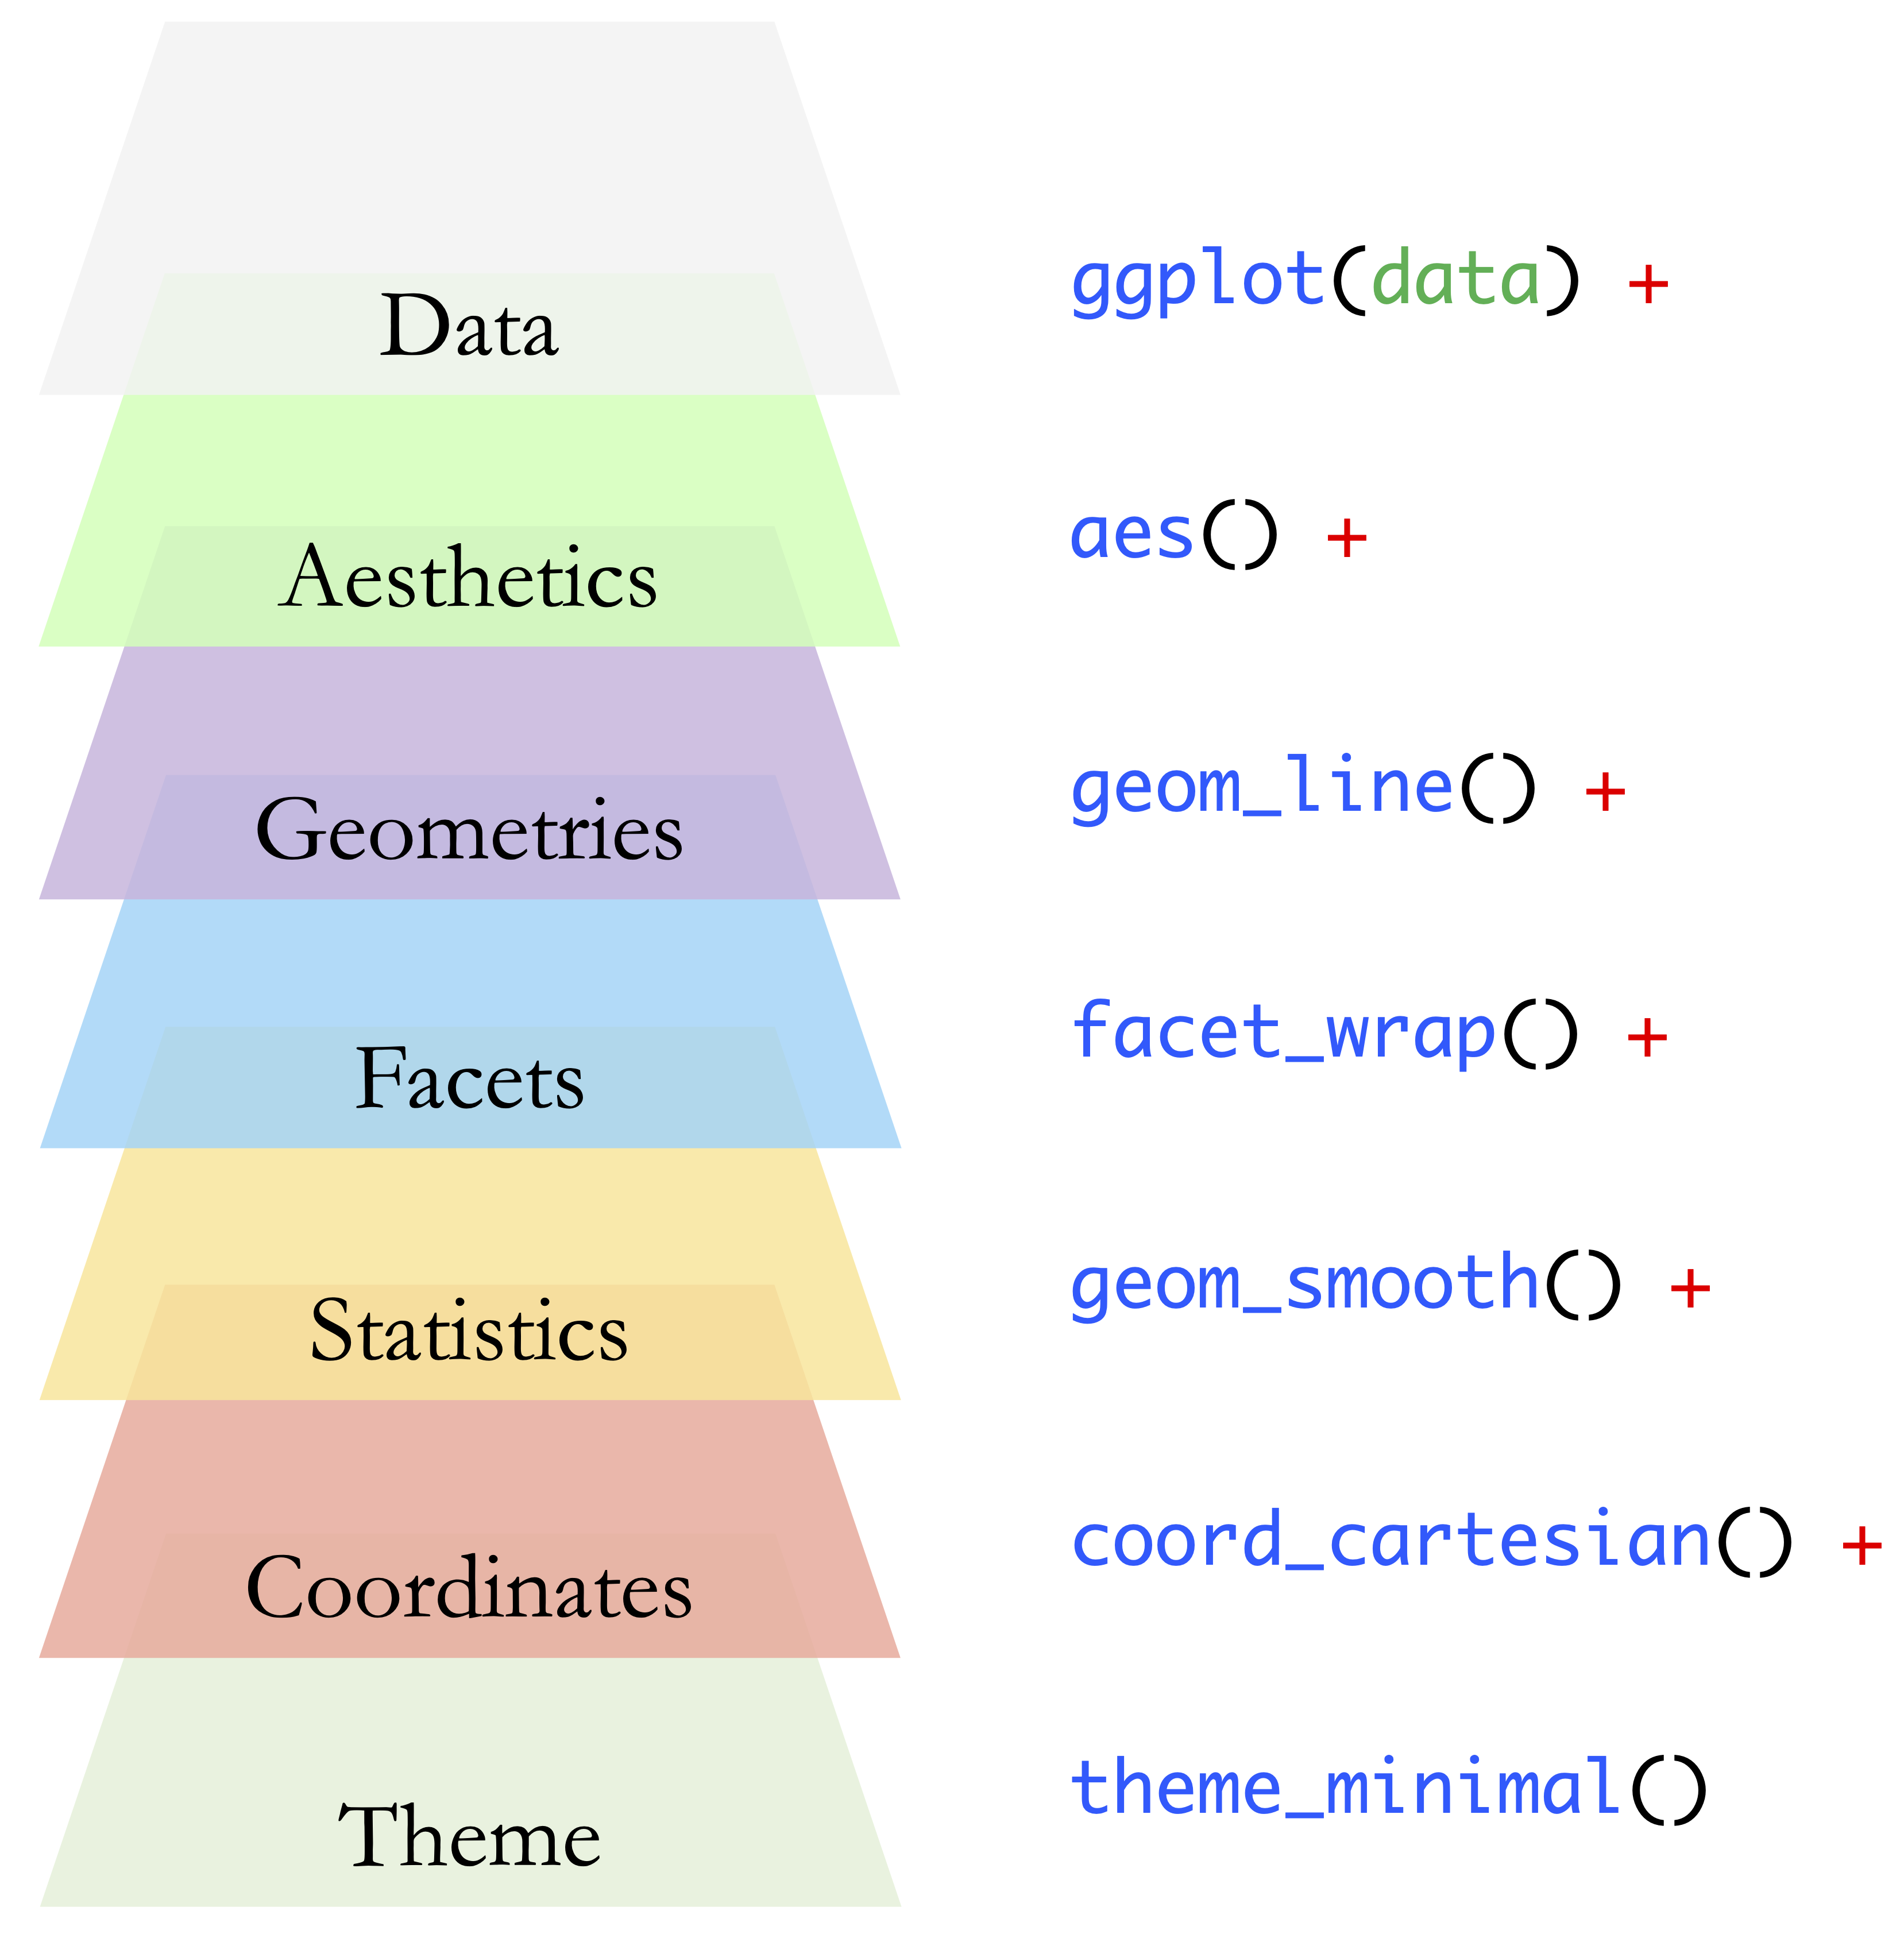
\includegraphics[width=0.85\linewidth,height=\textheight,keepaspectratio]{images/ch1_ggplot_layers.png}

}

\caption{\label{fig-ggplot-layes}Grammar of Graphics and ggplot2 layers.
The seven core layers of a ggplot: data, aesthetics, geometries, facets,
statistics, coordinates, and theme.}

\end{figure}%

Before using \textbf{ggplot2}, install the package as described in
Section \ref{sec-install-packages}, then load it into your session:

\begin{Shaded}
\begin{Highlighting}[]
\FunctionTok{library}\NormalTok{(ggplot2)}
\end{Highlighting}
\end{Shaded}

To see these ideas in action, consider the following simple scatter plot
of miles per gallon (\texttt{mpg}) versus horsepower (\texttt{hp}) using
the built-in \emph{mtcars} dataset:

\begin{Shaded}
\begin{Highlighting}[]
\FunctionTok{ggplot}\NormalTok{(}\AttributeTok{data =}\NormalTok{ mtcars) }\SpecialCharTok{+}
  \FunctionTok{geom\_point}\NormalTok{(}\AttributeTok{mapping =} \FunctionTok{aes}\NormalTok{(}\AttributeTok{x =}\NormalTok{ mpg, }\AttributeTok{y =}\NormalTok{ hp))}
\end{Highlighting}
\end{Shaded}

\begin{center}
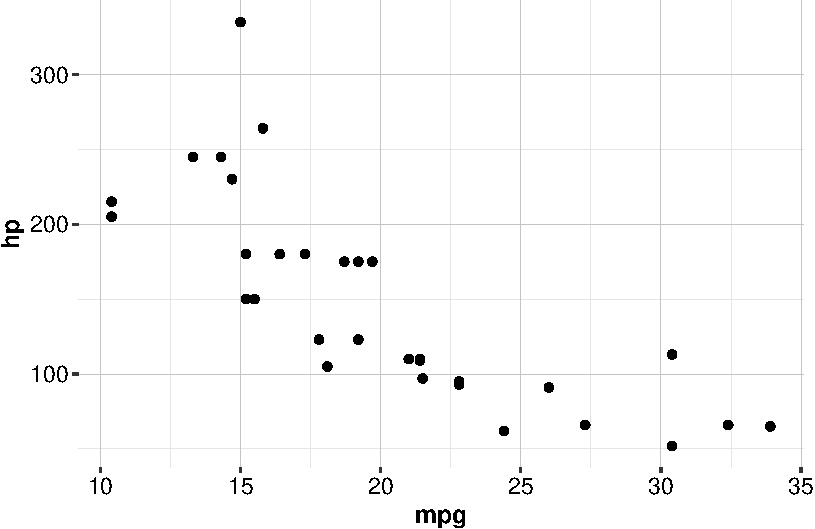
\includegraphics[width=0.65\linewidth,height=\textheight,keepaspectratio]{1-Intro-R_files/figure-pdf/unnamed-chunk-53-1.pdf}
\end{center}

In this example:

\begin{itemize}
\item
  \texttt{ggplot(data\ =\ mtcars)} initializes the plot with the
  dataset;
\item
  \texttt{geom\_point()} adds a layer of points;
\item
  \texttt{aes()} defines the aesthetic mapping from variables to axes.
\end{itemize}

The general template for \textbf{ggplot2} plots is:

\begin{Shaded}
\begin{Highlighting}[]
\FunctionTok{ggplot}\NormalTok{(}\AttributeTok{data =} \SpecialCharTok{\textless{}}\NormalTok{DATA}\SpecialCharTok{\textgreater{}}\NormalTok{) }\SpecialCharTok{+}
  \ErrorTok{\textless{}}\NormalTok{GEOM\_FUNCTION}\SpecialCharTok{\textgreater{}}\NormalTok{(}\AttributeTok{mapping =} \FunctionTok{aes}\NormalTok{(}\SpecialCharTok{\textless{}}\NormalTok{MAPPINGS}\SpecialCharTok{\textgreater{}}\NormalTok{))}
\end{Highlighting}
\end{Shaded}

Replace the angle brackets with your own inputs. This template provides
a consistent framework for building plots incrementally, adding layers
such as smoothing lines, facets, or custom themes. You will use this
approach throughout the book to explore, analyze, and communicate
insights from your data.

\subsection*{Geom Functions in ggplot2}\label{geom-functions-in-ggplot2}
\addcontentsline{toc}{subsection}{Geom Functions in ggplot2}

In \textbf{ggplot2}, \emph{geom functions} define what kind of plot you
want to make. Each \texttt{geom\_} function adds a \emph{geometric
object}, such as points, lines, or bars, as a new layer on top of your
plot.

Here are some of the most commonly used geom functions:

\begin{itemize}
\tightlist
\item
  \texttt{geom\_point()} creates a scatter plot;
\item
  \texttt{geom\_bar()} creates a bar chart;
\item
  \texttt{geom\_line()} creates a line chart;
\item
  \texttt{geom\_boxplot()} creates a box plot;
\item
  \texttt{geom\_histogram()} creates a histogram;
\item
  \texttt{geom\_density()} creates a smooth density curve;
\item
  \texttt{geom\_smooth()} adds a smoothed trend line (e.g., LOESS or
  linear fit).
\end{itemize}

For example, to visualize the relationship between miles per gallon
(\texttt{mpg}) and horsepower (\texttt{hp}) in the \emph{mtcars} dataset
using a smoothed trend line:

\begin{Shaded}
\begin{Highlighting}[]
\FunctionTok{ggplot}\NormalTok{(}\AttributeTok{data =}\NormalTok{ mtcars) }\SpecialCharTok{+}
  \FunctionTok{geom\_smooth}\NormalTok{(}\AttributeTok{mapping =} \FunctionTok{aes}\NormalTok{(}\AttributeTok{x =}\NormalTok{ mpg, }\AttributeTok{y =}\NormalTok{ hp))}
\end{Highlighting}
\end{Shaded}

\begin{center}
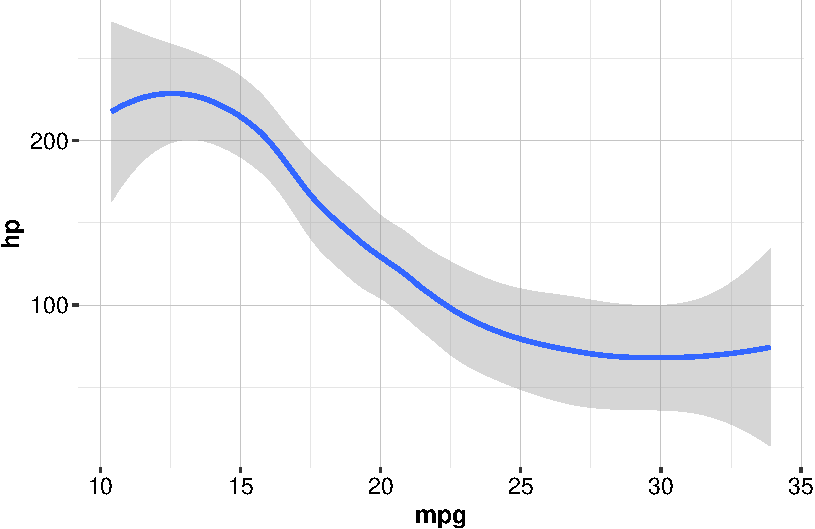
\includegraphics[width=0.65\linewidth,height=\textheight,keepaspectratio]{1-Intro-R_files/figure-pdf/unnamed-chunk-55-1.pdf}
\end{center}

This plot shows the general pattern in the data, helping you see whether
\texttt{mpg} tends to increase or decrease as \texttt{hp} changes.

You can also \emph{combine multiple geoms} to enrich your plots. For
instance, layering a scatter plot with a smooth trend line:

\begin{Shaded}
\begin{Highlighting}[]
\FunctionTok{ggplot}\NormalTok{(}\AttributeTok{data =}\NormalTok{ mtcars) }\SpecialCharTok{+}
  \FunctionTok{geom\_smooth}\NormalTok{(}\AttributeTok{mapping =} \FunctionTok{aes}\NormalTok{(}\AttributeTok{x =}\NormalTok{ mpg, }\AttributeTok{y =}\NormalTok{ hp)) }\SpecialCharTok{+} 
  \FunctionTok{geom\_point}\NormalTok{(}\AttributeTok{mapping =} \FunctionTok{aes}\NormalTok{(}\AttributeTok{x =}\NormalTok{ mpg, }\AttributeTok{y =}\NormalTok{ hp))}
\end{Highlighting}
\end{Shaded}

\begin{center}
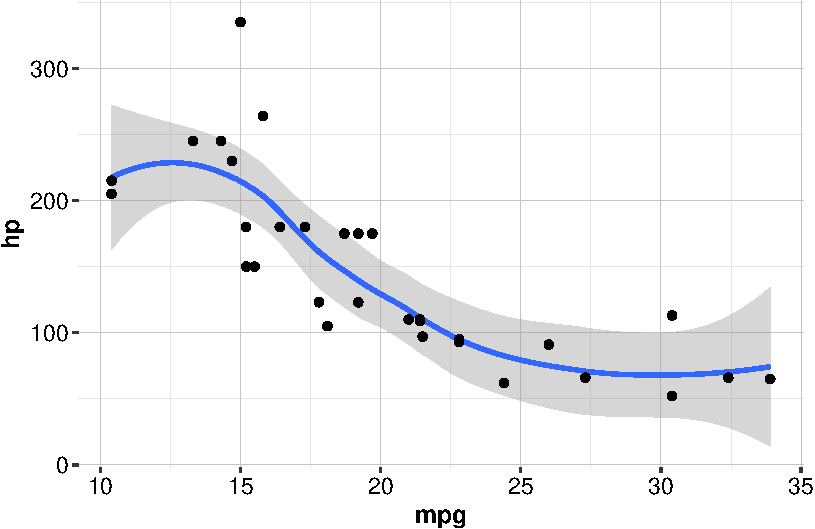
\includegraphics[width=0.65\linewidth,height=\textheight,keepaspectratio]{1-Intro-R_files/figure-pdf/unnamed-chunk-56-1.pdf}
\end{center}

The order of layers matters: here, the trend line is plotted first, and
the points are layered on top. This lets you preserve visibility while
showing both the data and the overall pattern.

If multiple layers use the same aesthetic mappings, you can define them
\emph{once globally} inside the \texttt{ggplot()} call:

\begin{Shaded}
\begin{Highlighting}[]
\FunctionTok{ggplot}\NormalTok{(}\AttributeTok{data =}\NormalTok{ mtcars, }\AttributeTok{mapping =} \FunctionTok{aes}\NormalTok{(}\AttributeTok{x =}\NormalTok{ mpg, }\AttributeTok{y =}\NormalTok{ hp)) }\SpecialCharTok{+}
  \FunctionTok{geom\_smooth}\NormalTok{() }\SpecialCharTok{+} 
  \FunctionTok{geom\_point}\NormalTok{()}
\end{Highlighting}
\end{Shaded}

This avoids repeating the same mapping in each layer and keeps your code
cleaner and more consistent.

\begin{quote}
\emph{Try it yourself}: Pick two numeric variables from the
\texttt{churn} dataset, for example, \texttt{day.mins} (Day Minutes) and
\texttt{eve.mins} (Evening Minutes). Use \texttt{geom\_point()} to
create a scatter plot. What relationship do you observe?
\end{quote}

\subsection*{Aesthetics in ggplot2}\label{aesthetics-in-ggplot2}
\addcontentsline{toc}{subsection}{Aesthetics in ggplot2}

\emph{Aesthetics} in \textbf{ggplot2} define how data variables are
visually mapped to features like color, size, shape, and transparency.
These mappings are specified inside the \texttt{aes()} function and
allow your plot to visually reflect differences in the data.

For example, to map the color of each point to the number of cylinders
in a car:

\begin{Shaded}
\begin{Highlighting}[]
\FunctionTok{ggplot}\NormalTok{(}\AttributeTok{data =}\NormalTok{ mtcars) }\SpecialCharTok{+}
  \FunctionTok{geom\_point}\NormalTok{(}\AttributeTok{mapping =} \FunctionTok{aes}\NormalTok{(}\AttributeTok{x =}\NormalTok{ mpg, }\AttributeTok{y =}\NormalTok{ hp, }\AttributeTok{color =}\NormalTok{ cyl))}
\end{Highlighting}
\end{Shaded}

\begin{center}
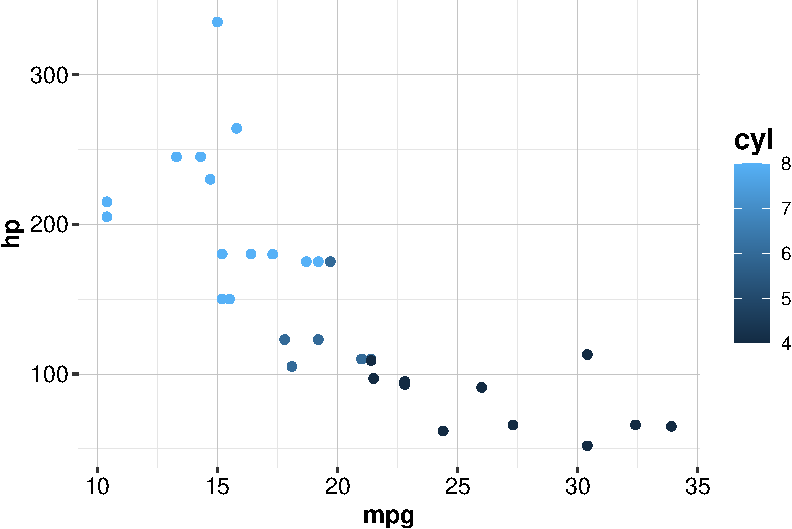
\includegraphics[width=0.65\linewidth,height=\textheight,keepaspectratio]{1-Intro-R_files/figure-pdf/unnamed-chunk-58-1.pdf}
\end{center}

Because \texttt{color\ =\ cyl} is inside \texttt{aes()}, the color is
\emph{data-driven}. Each point's color corresponds to the number of
cylinders (\texttt{cyl}), and \textbf{ggplot2} automatically adds a
legend.

Other aesthetics you can vary include \texttt{size}, \texttt{alpha}
(transparency), and \texttt{shape}:

\begin{Shaded}
\begin{Highlighting}[]
\CommentTok{\# Varying point size by number of cylinders}
\FunctionTok{ggplot}\NormalTok{(}\AttributeTok{data =}\NormalTok{ mtcars) }\SpecialCharTok{+}
  \FunctionTok{geom\_point}\NormalTok{(}\AttributeTok{mapping =} \FunctionTok{aes}\NormalTok{(}\AttributeTok{x =}\NormalTok{ mpg, }\AttributeTok{y =}\NormalTok{ hp, }\AttributeTok{size =}\NormalTok{ cyl))}

\CommentTok{\# Varying transparency (alpha) by number of cylinders}
\FunctionTok{ggplot}\NormalTok{(}\AttributeTok{data =}\NormalTok{ mtcars) }\SpecialCharTok{+}
  \FunctionTok{geom\_point}\NormalTok{(}\AttributeTok{mapping =} \FunctionTok{aes}\NormalTok{(}\AttributeTok{x =}\NormalTok{ mpg, }\AttributeTok{y =}\NormalTok{ hp, }\AttributeTok{alpha =}\NormalTok{ cyl))}
\end{Highlighting}
\end{Shaded}

\begin{figure}

\begin{minipage}{0.50\linewidth}
\begin{center}
\pandocbounded{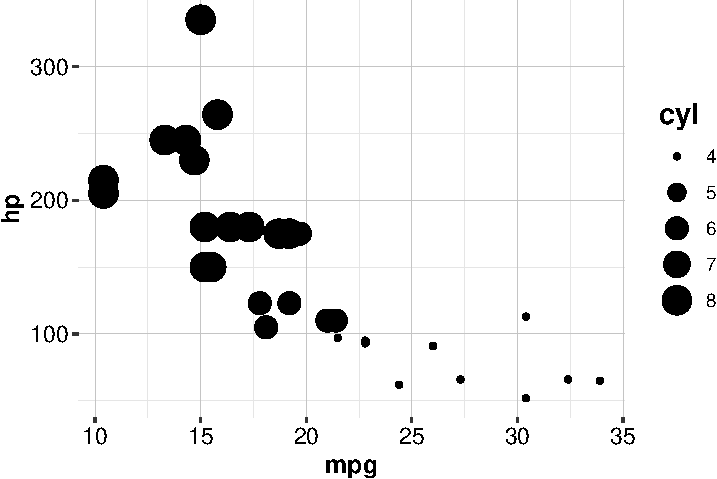
\includegraphics[keepaspectratio]{1-Intro-R_files/figure-pdf/unnamed-chunk-59-1.pdf}}
\end{center}
\end{minipage}%
%
\begin{minipage}{0.50\linewidth}
\begin{center}
\pandocbounded{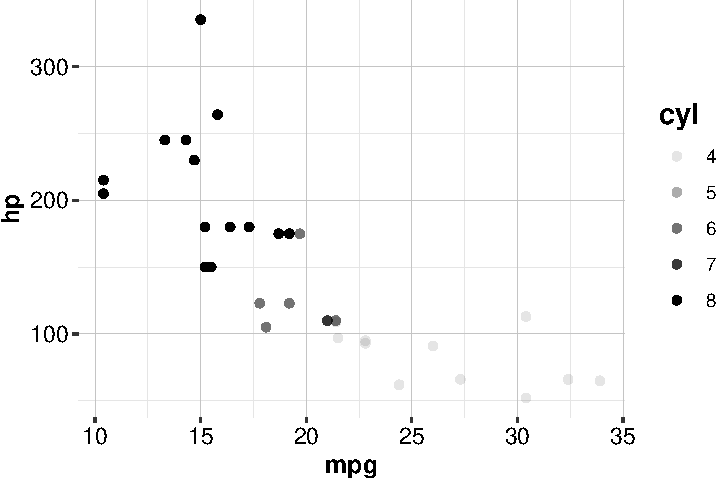
\includegraphics[keepaspectratio]{1-Intro-R_files/figure-pdf/unnamed-chunk-59-2.pdf}}
\end{center}
\end{minipage}%

\end{figure}%

When aesthetics are placed \emph{inside} \texttt{aes()}, they respond to
the data. If you want to apply a constant appearance, such as making all
points blue or triangles of the same size, set the attributes
\emph{outside} of \texttt{aes()}:

\begin{Shaded}
\begin{Highlighting}[]
\FunctionTok{ggplot}\NormalTok{(}\AttributeTok{data =}\NormalTok{ mtcars) }\SpecialCharTok{+}
  \FunctionTok{geom\_point}\NormalTok{(}\AttributeTok{mapping =} \FunctionTok{aes}\NormalTok{(}\AttributeTok{x =}\NormalTok{ mpg, }\AttributeTok{y =}\NormalTok{ hp),}
             \AttributeTok{color =} \StringTok{"blue"}\NormalTok{, }\AttributeTok{size =} \DecValTok{3}\NormalTok{, }\AttributeTok{shape =} \DecValTok{2}\NormalTok{)}
\end{Highlighting}
\end{Shaded}

\begin{center}
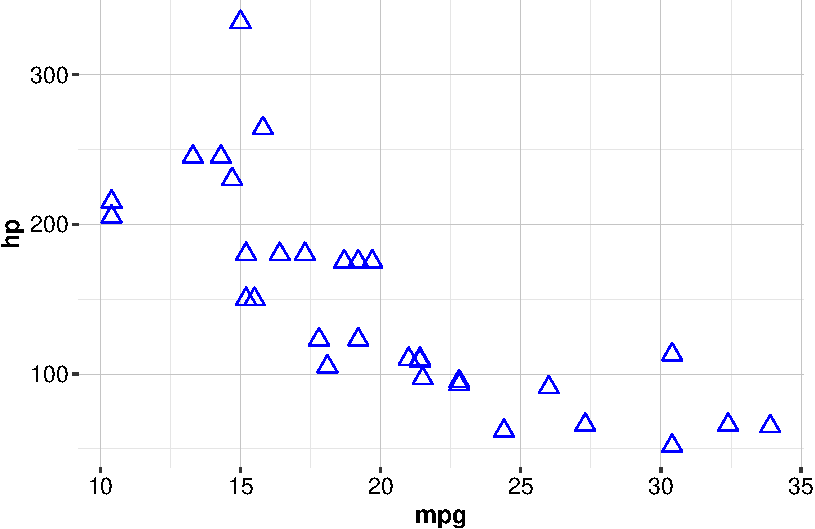
\includegraphics[width=0.65\linewidth,height=\textheight,keepaspectratio]{1-Intro-R_files/figure-pdf/unnamed-chunk-60-1.pdf}
\end{center}

This creates a plot with fixed styling: all points are blue, triangular,
and equally sized. Since the appearance is not based on the data,
\textbf{ggplot2} does not generate a legend.

\begin{quote}
\emph{Try it yourself}: In the \texttt{churn} dataset, can you map color
to the \texttt{churn} variable and size to \texttt{custserv.calls} in a
scatter plot of \texttt{day.mins} versus \texttt{eve.mins}? What do you
observe?
\end{quote}

With just a few core components, such as \texttt{geom\_point()},
\texttt{geom\_smooth()}, and \texttt{aes()}, you can construct
expressive and insightful graphics. In Chapter \ref{sec-ch4-EDA}, we
will expand on this foundation to explore distributions, relationships,
and trends as part of the EDA process.

For more details, see the
\href{https://ggplot2.tidyverse.org}{\textbf{ggplot2} documentation}. If
you are curious about interactive visualizations, check out packages
like \href{https://plotly.com/r}{\textbf{plotly}} or
\href{https://CRAN.R-project.org/package=shiny}{\textbf{Shiny}}.

\section{Formula in R}\label{sec-formula-in-R}

Formulas in R offer a simple and powerful way to describe relationships
between variables. They are used extensively in statistical modeling,
especially for regression, classification, and machine learning, to
define how an outcome depends on one or more predictors.

A formula in R uses the tilde symbol \texttt{\textasciitilde{}} to
separate the response variable (on the left) from the predictor
variables (on the right). The basic structure looks like this:

\begin{Shaded}
\begin{Highlighting}[]
\NormalTok{response }\SpecialCharTok{\textasciitilde{}}\NormalTok{ predictor1 }\SpecialCharTok{+}\NormalTok{ predictor2 }\SpecialCharTok{+}\NormalTok{ ...}
\end{Highlighting}
\end{Shaded}

For example, in the \texttt{diamonds} dataset, you could model
\texttt{price} as a function of \texttt{carat}, \texttt{cut}, and
\texttt{color} using:

\begin{Shaded}
\begin{Highlighting}[]
\NormalTok{price }\SpecialCharTok{\textasciitilde{}}\NormalTok{ carat }\SpecialCharTok{+}\NormalTok{ cut }\SpecialCharTok{+}\NormalTok{ color}
\end{Highlighting}
\end{Shaded}

To include \emph{all} other variables in the dataset as predictors, you
can use a shorthand formula:

\begin{Shaded}
\begin{Highlighting}[]
\NormalTok{price }\SpecialCharTok{\textasciitilde{}}\NormalTok{ .}
\end{Highlighting}
\end{Shaded}

This is especially useful when working with large datasets where listing
every predictor manually would be inefficient.

Behind the scenes, an R formula acts as a \emph{symbolic object}. Rather
than computing anything immediately, it instructs R to interpret
variable names as columns in a dataset, making your modeling code both
readable and flexible.

Conceptually, the left-hand side of \texttt{\textasciitilde{}}
represents the \emph{response} variable (what you want to predict), and
the right-hand side lists the \emph{predictors} (what you use to predict
it). Mathematically, this can be thought of as:

\[
y = f(x_1, x_2, \dots)
\]

Here is a quick example using linear regression. Suppose we want to
predict a diamond's price based on three features:

\begin{Shaded}
\begin{Highlighting}[]
\NormalTok{model }\OtherTok{\textless{}{-}} \FunctionTok{lm}\NormalTok{(price }\SpecialCharTok{\textasciitilde{}}\NormalTok{ carat }\SpecialCharTok{+}\NormalTok{ cut }\SpecialCharTok{+}\NormalTok{ color, }\AttributeTok{data =}\NormalTok{ diamonds)}
\end{Highlighting}
\end{Shaded}

In this case, the formula defines the model structure, while the
\texttt{data} argument tells R which dataset to use.

You will encounter formulas repeatedly throughout the book in regression
models, classification algorithms, and other statistical methods (see
Chapters \ref{sec-ch7-classification-knn}, \ref{sec-ch9-bayes}, and
\ref{sec-ch10-regression}). Learning this syntax early will help you
build, interpret, and adjust models more effectively later on.

\begin{quote}
\emph{Try it yourself}: Using the \texttt{diamonds} dataset, try fitting
a model where \texttt{price} depends on \texttt{carat} and
\texttt{clarity}. What happens if you use
\texttt{price\ \textasciitilde{}\ .} instead?
\end{quote}

\section{Simulating Data in R}\label{sec-ch1-simulate-data}

Some readers find simulation unfamiliar at first and may be tempted to
skip this section. However, it is one of the most practical and
empowering tools in data science. With just a few lines of code, you can
generate realistic datasets to explore statistical concepts, test
algorithms, or build examples when real data is unavailable.

In R, simulation is used extensively for both learning and modeling. It
plays a key role in prototyping and debugging algorithms, teaching and
illustrating statistical principles, generating synthetic datasets for
model development, and testing methods under controlled, reproducible
conditions.

R offers many built-in functions to generate random values from common
statistical distributions. Some of the most frequently used include:

\begin{itemize}
\tightlist
\item
  \texttt{rnorm(n,\ mean,\ sd)}: normal distribution (e.g., for heights
  or test scores),
\item
  \texttt{runif(n,\ min,\ max)}: uniform distribution (e.g., for
  probabilities or noise),
\item
  \texttt{rbinom(n,\ size,\ prob)}: binomial distribution (e.g., yes/no
  outcomes),
\item
  \texttt{rexp(n,\ rate)}: exponential distribution (e.g., for
  time-to-event data),
\item
  \texttt{sample(x,\ size,\ replace)}: sampling from a vector (e.g.,
  categories or IDs).
\end{itemize}

To make your results reproducible, always use \texttt{set.seed()} before
generating random values.

\phantomsection\label{ex-simulate-normal}
\textbf{Example}: Simulate 500 values from a normal distribution with
mean 10 and standard deviation 2.

\begin{Shaded}
\begin{Highlighting}[]
\FunctionTok{set.seed}\NormalTok{(}\DecValTok{42}\NormalTok{)}

\NormalTok{x }\OtherTok{\textless{}{-}} \FunctionTok{rnorm}\NormalTok{(}\AttributeTok{n =} \DecValTok{500}\NormalTok{, }\AttributeTok{mean =} \DecValTok{10}\NormalTok{, }\AttributeTok{sd =} \DecValTok{2}\NormalTok{)}

\FunctionTok{summary}\NormalTok{(x)}
\NormalTok{      Min. }\DecValTok{1}\NormalTok{st Qu.  Median    Mean }\DecValTok{3}\NormalTok{rd Qu.    Max. }
     \FloatTok{4.014}   \FloatTok{8.679}   \FloatTok{9.924}   \FloatTok{9.940}  \FloatTok{11.271}  \FloatTok{15.932}

\FunctionTok{ggplot}\NormalTok{(}\FunctionTok{data.frame}\NormalTok{(x)) }\SpecialCharTok{+}
  \FunctionTok{geom\_histogram}\NormalTok{(}\FunctionTok{aes}\NormalTok{(}\AttributeTok{x =}\NormalTok{ x), }\AttributeTok{color =} \StringTok{"white"}\NormalTok{, }\AttributeTok{fill =} \StringTok{"\#2C7BB6"}\NormalTok{, }\AttributeTok{bins =} \DecValTok{30}\NormalTok{) }\SpecialCharTok{+}
  \FunctionTok{labs}\NormalTok{(}\AttributeTok{title =} \StringTok{"Distribution of Simulated Data"}\NormalTok{, }\AttributeTok{x =} \StringTok{"Values"}\NormalTok{, }\AttributeTok{y =} \StringTok{"Frequency"}\NormalTok{) }
\end{Highlighting}
\end{Shaded}

\begin{center}
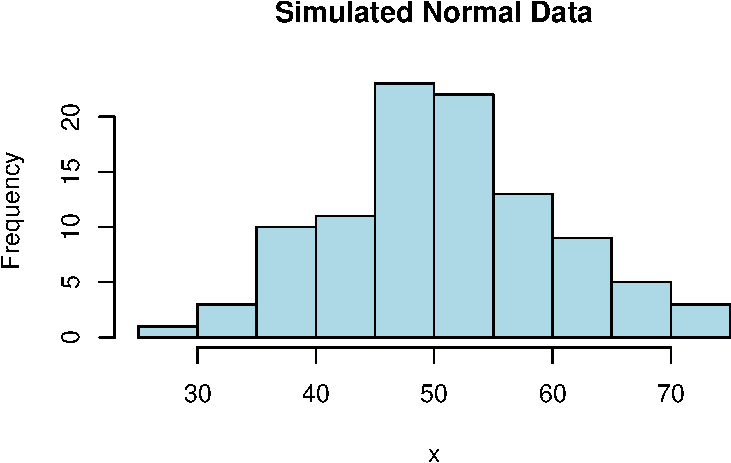
\includegraphics[width=0.6\linewidth,height=\textheight,keepaspectratio]{1-Intro-R_files/figure-pdf/unnamed-chunk-64-1.pdf}
\end{center}

You can also simulate multiple variables and combine them into a data
frame to create small, realistic datasets.

\phantomsection\label{ex-simulate-patients}
\textbf{Example}: Create synthetic data for a small study on age and
blood pressure.

\begin{Shaded}
\begin{Highlighting}[]
\FunctionTok{set.seed}\NormalTok{(}\DecValTok{42}\NormalTok{)}

\NormalTok{age }\OtherTok{\textless{}{-}} \FunctionTok{sample}\NormalTok{(}\DecValTok{30}\SpecialCharTok{:}\DecValTok{80}\NormalTok{, }\DecValTok{50}\NormalTok{, }\AttributeTok{replace =} \ConstantTok{TRUE}\NormalTok{)}
\NormalTok{bp  }\OtherTok{\textless{}{-}} \FunctionTok{rnorm}\NormalTok{(}\DecValTok{50}\NormalTok{, }\AttributeTok{mean =} \DecValTok{120}\NormalTok{, }\AttributeTok{sd =} \DecValTok{15}\NormalTok{)}

\NormalTok{patients }\OtherTok{\textless{}{-}} \FunctionTok{data.frame}\NormalTok{(}\AttributeTok{age =}\NormalTok{ age, }\AttributeTok{blood\_pressure =}\NormalTok{ bp)}

\FunctionTok{head}\NormalTok{(patients)}
\NormalTok{     age blood\_pressure}
   \DecValTok{1}  \DecValTok{78}       \FloatTok{93.55255}
   \DecValTok{2}  \DecValTok{66}      \FloatTok{126.90146}
   \DecValTok{3}  \DecValTok{30}      \FloatTok{110.40008}
   \DecValTok{4}  \DecValTok{54}      \FloatTok{126.83175}
   \DecValTok{5}  \DecValTok{39}      \FloatTok{130.57256}
   \DecValTok{6}  \DecValTok{65}      \FloatTok{135.52655}
\end{Highlighting}
\end{Shaded}

Simulation is more than a teaching device; it is foundational in
advanced techniques such as bootstrapping, Bayesian inference, and Monte
Carlo methods. In this book (e.g., Chapter
\ref{sec-ch7-classification-knn}), you will use simulated data to
explore and evaluate models with clarity and control.

\begin{quote}
\emph{Try it yourself}: Simulate a dataset with 100 people. Assign each
an \texttt{age} between 18 and 65, and an \texttt{income} drawn from a
normal distribution with mean 40,000 and standard deviation 8,000. Can
you visualize the income distribution using a histogram? What does a
scatter plot of income vs.~age reveal?
\end{quote}

\section{Reporting with R Markdown}\label{reporting-with-r-markdown}

Imagine you have just completed an in-depth analysis. Your model
predicts customer churn with 87\% accuracy, the visualizations are
compelling, and the insights could inform real business decisions. Now
comes a crucial question: how will you present your findings?

Communicating insights is one of the most important, yet often
overlooked, steps in the Data Science Workflow. Analyses that are
statistically sound and computationally rigorous have limited value if
their conclusions are not conveyed clearly. Whether addressing technical
collaborators, business stakeholders, or policymakers, you must
transform complex results into a format that is both accessible and
reproducible.

R Markdown is designed for this purpose. It provides a flexible and
powerful environment for integrating code, output, and narrative in a
single document. With R Markdown, you can weave together your analysis
and explanation, producing reports, presentations, or dashboards that
update automatically as your data changes.

This book was initially drafted entirely using R Markdown in combination
with the \href{https://bookdown.org}{\textbf{bookdown}} package. This
enabled automated output generation, version control integration, and
full synchronization of code, figures, and tables, ensuring that every
result remains accurate and reproducible across versions.

Unlike traditional word processors, R Markdown supports dynamic content.
Reports compiled from \texttt{.Rmd} files are not just documents; they
are living, executable records of your analysis. Supported output
formats include HTML, PDF, Word, and PowerPoint, allowing you to tailor
your communication to different audiences. With the addition of
\textbf{Shiny}, R Markdown can even produce interactive dashboards for
real-time data exploration.

If you are new to R Markdown, two official resources provide practical
and accessible starting points. The
\href{https://rstudio.com/wp-content/uploads/2016/03/rmarkdown-cheatsheet-2.0.pdf}{\emph{R
Markdown Cheat Sheet}}, also available in RStudio under \emph{Help
\textgreater{} Cheatsheets}, offers a concise overview of key syntax and
features. For more advanced formatting and customization, the
\href{https://rstudio.com/wp-content/uploads/2015/03/rmarkdown-reference.pdf}{\emph{R
Markdown Reference Guide}} provides detailed documentation and examples.

\begin{quote}
\emph{Try it yourself}: Open RStudio, create a new R Markdown file, and
type your first heading and code chunk. With just a few lines, you can
generate a fully formatted HTML report that combines your analysis and
your voice.
\end{quote}

\subsection*{R Markdown Basics}\label{r-markdown-basics}
\addcontentsline{toc}{subsection}{R Markdown Basics}

How can you share an analysis that includes your code, reasoning, and
results all organized in one place? This is the principle of
\emph{literate programming}, where code and narrative are integrated
within a single document. R Markdown embraces this approach, enabling
you to combine text, executable R code, and visual output in a fully
reproducible format.

Unlike word processors that display formatting directly as you type, R
Markdown separates content creation from rendering. You write in plain
text and compile the document to produce the final output. During this
process, R runs the code chunks, generates figures and tables, and
inserts them automatically into the report. This workflow ensures that
your narrative and results remain synchronized, even as the data
changes.

To create a new R Markdown file in RStudio, navigate to:

\begin{quote}
\emph{File \textgreater{} New File \textgreater{} R Markdown}
\end{quote}

A dialog box will appear where you can choose the type of document you
want to create. For a standard report, select ``Document.'' Other
options include ``Presentation'' for slides, ``Shiny'' for interactive
applications, and ``From Template'' for preconfigured formats. After
entering a title and author name, choose the desired output format:
HTML, PDF, or Word. HTML is typically recommended for beginners, as it
compiles quickly and provides useful feedback during development.

R Markdown files use the \texttt{.Rmd} extension, distinguishing them
from standard \texttt{.R} scripts. Each new file includes a built-in
template that you can modify with your own text, code, and formatting.
This serves as a useful starting point for learning the structure and
syntax of R Markdown documents.

\begin{quote}
\emph{Try it yourself}: Create a new R Markdown file and render it
without changing anything. Then edit the title, add your own sentence,
and run it again to see how the output updates.
\end{quote}

\subsection*{The Header}\label{the-header}
\addcontentsline{toc}{subsection}{The Header}

At the top of every R Markdown file is a section called the \emph{YAML
header}, which serves as the control panel for your document. It
contains metadata that determines how the document is rendered, such as
the title, author, date, and output format. This header is enclosed
between three dashes (\texttt{-\/-\/-}) at the beginning of the file.

Here is a typical example:

\begin{Shaded}
\begin{Highlighting}[]
\PreprocessorTok{{-}{-}{-}}
\FunctionTok{title}\KeywordTok{:}\AttributeTok{ }\StringTok{"Data Science is Cool"}
\FunctionTok{author}\KeywordTok{:}\AttributeTok{ }\StringTok{"Your Name"}
\FunctionTok{date}\KeywordTok{:}\AttributeTok{ }\StringTok{"June 01, 2025"}
\FunctionTok{output}\KeywordTok{:}\AttributeTok{ html\_document}
\PreprocessorTok{{-}{-}{-}}
\end{Highlighting}
\end{Shaded}

Each entry specifies a key element of the report:

\begin{itemize}
\item
  \texttt{title}: sets the title displayed at the top of the document.
\item
  \texttt{author}: identifies the report's author.
\item
  \texttt{date}: records the creation or compilation date.
\item
  \texttt{output}: defines the output format, such as
  \texttt{html\_document}, \texttt{pdf\_document}, or
  \texttt{word\_document}.
\end{itemize}

Additional customization options can be added to the header. For
instance, to include a table of contents in an HTML report, you can
modify the \texttt{output} field as follows:

\begin{Shaded}
\begin{Highlighting}[]
\FunctionTok{output}\KeywordTok{:}
\AttributeTok{  }\FunctionTok{html\_document}\KeywordTok{:}
\AttributeTok{    }\FunctionTok{toc}\KeywordTok{:}\AttributeTok{ }\CharTok{true}
\end{Highlighting}
\end{Shaded}

This is especially useful for longer documents with multiple sections,
allowing readers to navigate more easily. Other options include setting
figure dimensions, enabling syntax highlighting, or selecting a document
theme. These settings offer precise control over both the appearance and
behavior of your report.

In the next section, you will learn how to include code in your report
and configure how it is displayed during rendering.

\subsection*{Code Chunks and Inline
Code}\label{code-chunks-and-inline-code}
\addcontentsline{toc}{subsection}{Code Chunks and Inline Code}

One of the defining features of R Markdown is its ability to weave
together code and narrative. This is accomplished through \emph{code
chunks} and \emph{inline code}, which allow you to embed executable R
commands directly within your report. As a result, your output, such as
tables, plots, and summaries, remains consistent with the underlying
code and data.

A code chunk is a block of code enclosed in triple backticks
(\texttt{\textasciigrave{}\textasciigrave{}\textasciigrave{}}) and
marked with a chunk header that specifies the language (in this case,
\texttt{\{r\}}). For example:

\begin{Shaded}
\begin{Highlighting}[]
\InformationTok{\textasciigrave{}\textasciigrave{}\textasciigrave{}\{r\}}
\InformationTok{2 + 3}
\InformationTok{\textasciigrave{}\textasciigrave{}\textasciigrave{}}
\end{Highlighting}
\end{Shaded}

\begin{verbatim}
   [1] 5
\end{verbatim}

When the document is rendered, R executes the code and inserts the
output at the appropriate location. Code chunks are commonly used for
data wrangling, statistical modeling, creating visualizations, and
running simulations.

To run individual chunks interactively in RStudio, click the \emph{Run}
button at the top of the chunk or press
\texttt{Ctrl\ +\ Shift\ +\ Enter}. See Figure \ref{fig-run-chunk} for a
visual reference.

\begin{figure}[H]

\centering{

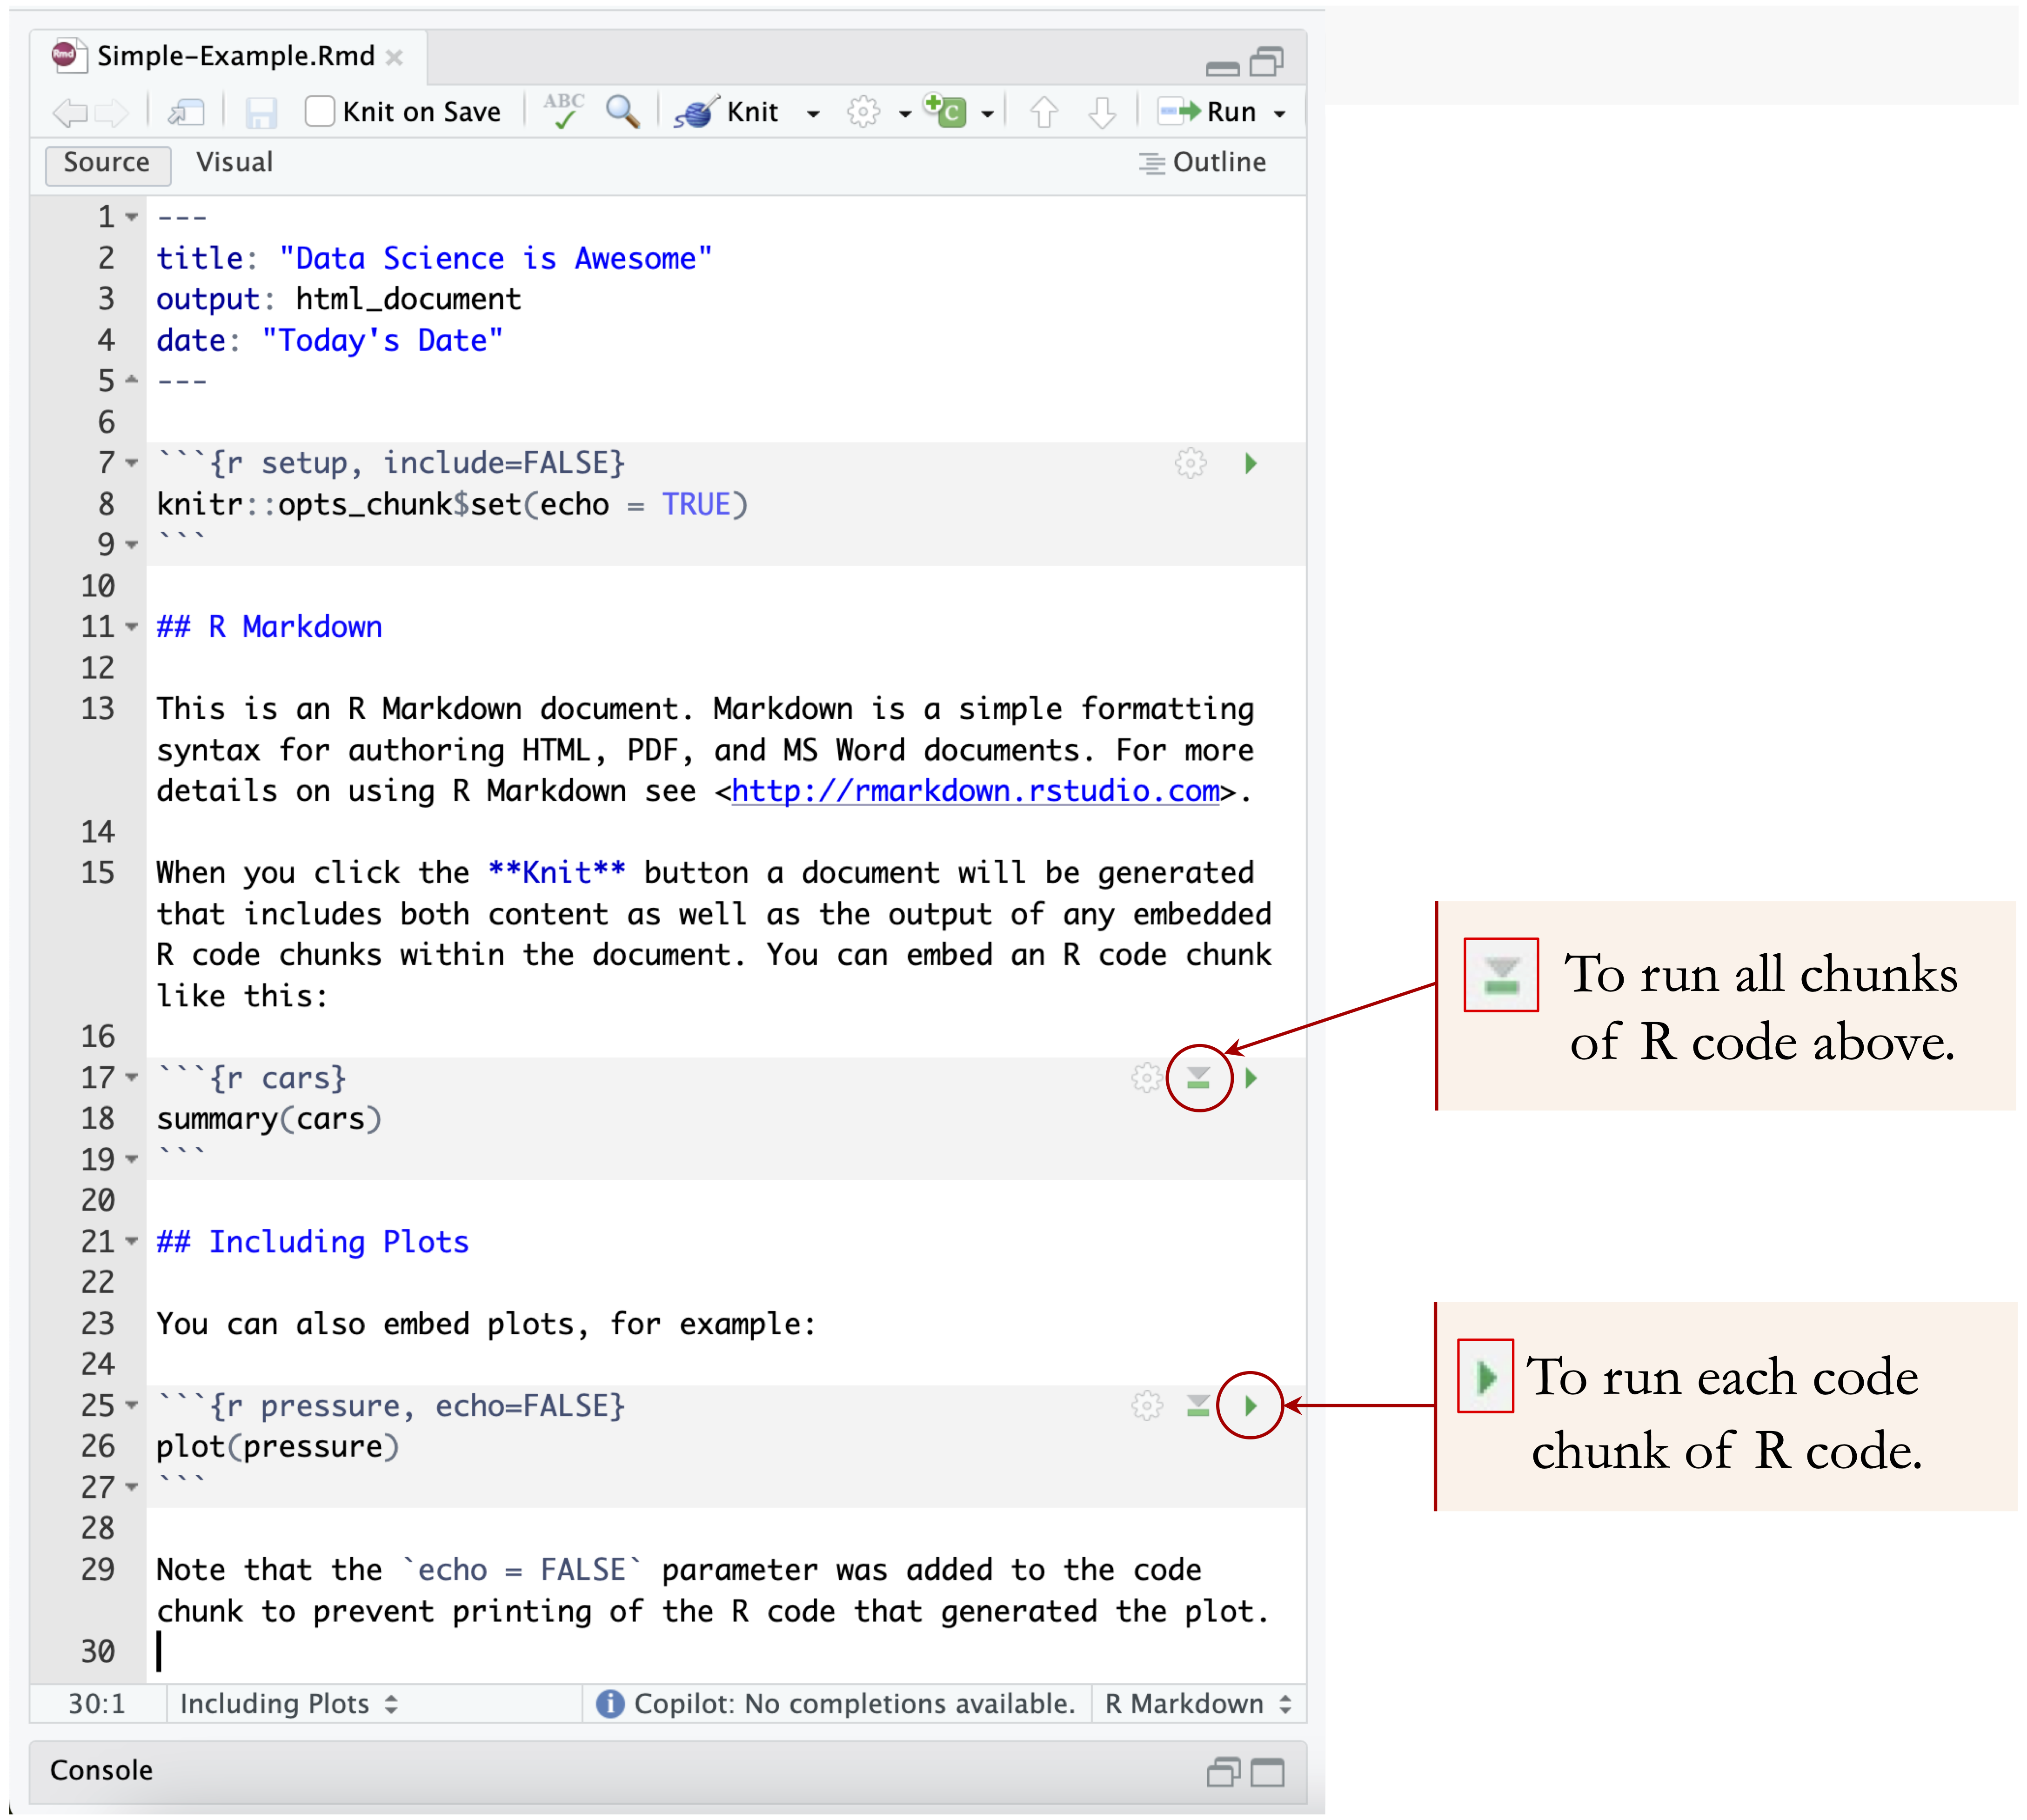
\includegraphics[width=0.75\linewidth,height=\textheight,keepaspectratio]{images/ch1_run-chunk.png}

}

\caption{\label{fig-run-chunk}Executing a code chunk in R Markdown using
the `Run' button in RStudio.}

\end{figure}%

Code chunks support a variety of options that control how code and
output are displayed. These options are specified in the chunk header.
For example:

\begin{itemize}
\item
  \texttt{echo\ =\ FALSE} hides the code but still displays the output.
\item
  \texttt{eval\ =\ FALSE} shows the code but does not execute it.
\item
  \texttt{message\ =\ FALSE} suppresses messages generated by functions
  (e.g., when loading packages).
\item
  \texttt{warning\ =\ FALSE} hides warning messages.
\item
  \texttt{error\ =\ FALSE} suppresses error messages.
\item
  \texttt{include\ =\ FALSE} runs the code but omits both the code and
  its output.
\end{itemize}

Table \ref{tbl-chunk-options} summarizes how these options affect what
appears in the final report:

\begin{table}

\caption{\label{tbl-chunk-options}Behavior of code chunk options and
their impact on execution, visibility, and outputs.}

\centering{

\centering
\resizebox{\ifdim\width>\linewidth\linewidth\else\width\fi}{!}{
\begin{tabular}{cccccccc}
\toprule
Option & Run Code & Show Code & Output & Plots & Messages & Warnings & Errors\\
\midrule
\texttt{echo = FALSE} & $\checkmark$ & $\times$ & $\checkmark$ & $\checkmark$ & $\checkmark$ & $\checkmark$ & $\checkmark$\\
\texttt{eval = FALSE} & $\times$ & $\checkmark$ & $\times$ & $\times$ & $\times$ & $\times$ & $\times$\\
\texttt{message = FALSE} & $\checkmark$ & $\checkmark$ & $\checkmark$ & $\checkmark$ & $\times$ & $\checkmark$ & $\checkmark$\\
\texttt{warning = FALSE} & $\checkmark$ & $\checkmark$ & $\checkmark$ & $\checkmark$ & $\checkmark$ & $\times$ & $\checkmark$\\
\texttt{error = FALSE} & $\checkmark$ & $\checkmark$ & $\checkmark$ & $\checkmark$ & $\checkmark$ & $\checkmark$ & $\times$\\
\addlinespace
\texttt{include = FALSE} & $\checkmark$ & $\times$ & $\times$ & $\times$ & $\times$ & $\times$ & $\times$\\
\bottomrule
\end{tabular}}

}

\end{table}%

In addition to full chunks, you can embed small pieces of R code
directly within text using \emph{inline code}. This is done with
backticks and the \texttt{r} prefix. For example:

\begin{quote}
The factorial of 5 is
\texttt{\textasciigrave{}r\ factorial(5)\textasciigrave{}}.
\end{quote}

This renders as:

\begin{quote}
The factorial of 5 is 120.
\end{quote}

Inline code is especially useful when you want to report dynamic values,
such as sample sizes, summary statistics, or dates, that update
automatically whenever the document is recompiled.

\begin{quote}
\emph{Try it yourself}: Create a new R Markdown file and add a code
chunk that calculates the mean of a numeric vector. Then use inline code
to display that mean in a sentence.
\end{quote}

\subsection*{Styling Text}\label{styling-text}
\addcontentsline{toc}{subsection}{Styling Text}

Clear, well-structured text is an essential part of any data report. In
R Markdown, you can format your writing to emphasize key ideas, organize
content, and improve readability. This section introduces a few core
formatting tools that help you communicate effectively.

To create section titles and organize your document, use one or more
\texttt{\#} symbols to indicate heading levels. For example, \texttt{\#}
creates a main section, \texttt{\#\#} a subsection, and so on. Bold text
is written by enclosing it in double asterisks (e.g.,
\texttt{**bold**}), while italic text uses single asterisks (e.g.,
\texttt{*italic*}). These conventions mirror common Markdown syntax and
work across all output formats.

Lists are created using \texttt{*} or \texttt{-} at the start of each
line. For example:

\begin{Shaded}
\begin{Highlighting}[]
\SpecialStringTok{* }\NormalTok{First item  }
\SpecialStringTok{* }\NormalTok{Second item}
\end{Highlighting}
\end{Shaded}

To insert hyperlinks, use square brackets for the link text followed by
the URL in parentheses, for example:
\texttt{{[}R\ Markdown\ website{]}(https://rmarkdown.rstudio.com)}. You
can also include images using a similar structure, with an exclamation
mark at the beginning: \texttt{!{[}Alt\ text{]}(path/to/image.png)}.

R Markdown supports mathematical notation using LaTeX-style syntax.
Inline equations are enclosed in single dollar signs, such as
\texttt{\$y\ =\ \textbackslash{}beta\_0\ +\ \textbackslash{}beta\_1\ x\$},
while block equations use double dollar signs and appear centered on
their own line:

\begin{Shaded}
\begin{Highlighting}[]
\AnnotationTok{Inline:}\CommentTok{ $y = \textbackslash{}beta\_0 + \textbackslash{}beta\_1 x$  }
\AnnotationTok{Block:}\CommentTok{ $$ y = \textbackslash{}beta\_0 + \textbackslash{}beta\_1 x $$}
\end{Highlighting}
\end{Shaded}

Mathematical expressions render correctly in HTML and PDF formats;
support in Word documents may be more limited.

For a full overview of Markdown formatting and additional options, see
the
\href{https://rstudio.com/wp-content/uploads/2016/03/rmarkdown-cheatsheet-2.0.pdf}{R
Markdown Cheat Sheet}.

\begin{quote}
\emph{Tip}: Try editing a heading, adding emphasis to a word, or
inserting a list in your own R Markdown document. Even small formatting
improvements can make your writing easier to follow.
\end{quote}

\subsection*{Mastering R Markdown}\label{mastering-r-markdown}
\addcontentsline{toc}{subsection}{Mastering R Markdown}

As your skills in R grow, R Markdown will become an increasingly
powerful tool, not only for reporting results but also for building
reproducible workflows that evolve with your projects. Mastery of this
tool enables you to document, share, and automate your analyses with
clarity and consistency.

Several resources can help you deepen your understanding. The online
book \href{https://bookdown.org/yihui/rmarkdown}{\emph{R Markdown: The
Definitive Guide}} provides a comprehensive reference, including
advanced formatting, customization options, and integration with tools
like \textbf{knitr} and \textbf{bookdown}. If you prefer structured
lessons, the \href{https://rmarkdown.rstudio.com/lesson-1.html}{R
Markdown tutorial series} offers a step-by-step introduction to
essential concepts and practices. For learners who enjoy interactive
platforms,
\href{https://www.datacamp.com/courses/reporting-with-r-markdown}{DataCamp's
R Markdown course} provides guided exercises. Finally, the
\href{https://community.rstudio.com/c/rmarkdown/9}{RStudio Community
forum} is an excellent place to find answers to specific questions and
engage with experienced users.

Throughout this book, you will continue using R Markdown, not just to
document isolated analyses, but to support entire data science
workflows. As your projects become more complex, this approach will help
ensure that your code, results, and conclusions remain transparent,
organized, and reproducible.

\section{Reporting with Quarto}\label{reporting-with-quarto}

While R Markdown has long been a popular tool for reproducible reporting
in R, Quarto represents its modern evolution. Designed to support
multilingual workflows, Quarto provides a unified framework for
combining narrative, code, and output across multiple programming
languages, including R, Python, Julia, and Observable JavaScript.

Like R Markdown, Quarto enables dynamic document generation. But it
extends these capabilities with enhanced support for cross-referencing,
equation numbering, citations, and a wide range of publishing formats,
including HTML, PDF, Word, slides, and websites, all from a single
\texttt{.qmd} file.

This book was originally drafted using R Markdown. However, once we
began developing a companion version in Python, we transitioned to
Quarto. Its language-agnostic design allowed us to maintain a consistent
workflow while supporting multiple programming languages in parallel.

If your work is primarily in R, R Markdown remains a mature and
well-supported tool. But if you use multiple languages, or plan to
create interactive documents, presentations, or websites, Quarto offers
a more flexible and forward-looking solution.

To create a new Quarto document in RStudio:

\begin{quote}
\emph{File \textgreater{} New File \textgreater{} Quarto Document}
\end{quote}

A dialog will prompt you to select the document type and programming
language. The syntax in \texttt{.qmd} files is similar to R Markdown,
making the transition smooth for most users.

To explore the full capabilities of Quarto, visit the official
documentation at \href{https://quarto.org}{\emph{quarto.org}}.

\section{Chapter Summary and
Takeaways}\label{chapter-summary-and-takeaways}

This chapter introduced the R programming language as the foundation for
data science and machine learning. You installed R and RStudio, explored
the RStudio interface, and executed your first commands. You also
learned how R handles core data types and structures, how to import and
examine real-world datasets, and how to visualize data effectively.

In addition, you were introduced to \emph{reproducible reporting} using
R Markdown and Quarto, two tools that integrate code, narrative, and
results in a single dynamic document. These tools support transparency,
collaboration, and long-term reproducibility, making them essential
components of the data science toolkit.

Throughout this chapter, we emphasized foundational habits:
\emph{writing clean code}, \emph{thinking systematically}, and
\emph{building scalable workflows}. These principles are essential at
every stage of the \emph{Data Science Workflow} and will serve as your
compass throughout this book. Many of my students begin their journey
with no prior programming experience. Yet by the end of the course, they
confidently use R to explore real-world datasets, create meaningful
visualizations, and draw actionable insights. If you are starting from
scratch; this path is entirely achievable. You are in good company.

\begin{quote}
\emph{Key takeaway}: Mastering R is not about memorization; it is about
developing a mindset for working with data. As illustrated in
Figure~\ref{fig-ch1-tiny-gains}, small, consistent improvements lead to
substantial progress. Do not worry if everything feels unfamiliar right
now. By working through the upcoming chapters step by step, you will
gradually build fluency and confidence in using R to analyze data and
communicate insights.
\end{quote}

Now that you have installed R, explored its key concepts, and visualized
data with \textbf{ggplot2}, it is time to apply what you have learned.

\section{Exercises}\label{sec-intro-R-exercises}

Use the exercises below to reinforce your understanding of the tools and
concepts introduced in this chapter. Begin with foundational tasks, then
build toward more complex data exploration and visualization challenges.

\begin{enumerate}
\def\labelenumi{\arabic{enumi}.}
\item
  Install R and RStudio on your computer.
\item
  Use \texttt{getwd()} to check your current working directory. Then use
  \texttt{setwd()} to change it to a location of your choice.
\item
  Create a numeric vector \texttt{numbers} with the values 5, 10, 15,
  20, and 25. Calculate its mean and standard deviation.
\item
  Use the \texttt{matrix()} function to construct a \(3 \times 4\)
  matrix filled with the numbers 1 through 12.
\item
  Build a data frame with the following columns:
\end{enumerate}

\begin{itemize}
\tightlist
\item
  \texttt{student\_id}: integer.
\item
  \texttt{name}: character.
\item
  \texttt{score}: numeric.
\item
  \texttt{passed}: logical (set to \texttt{TRUE} or \texttt{FALSE}).
\end{itemize}

Display the first few rows using \texttt{head()}.

\begin{enumerate}
\def\labelenumi{\arabic{enumi}.}
\setcounter{enumi}{5}
\item
  Install and load the \textbf{liver} and \textbf{ggplot2} packages. If
  installation fails, check your internet connection and CRAN access.
\item
  Load the \texttt{churn} dataset from the \textbf{liver} package.
  Display the first six rows with \texttt{head()}.
\item
  Use \texttt{str()} to inspect the structure of the \texttt{churn}
  dataset, and identify its variable types.
\item
  Use \texttt{dim()} to report the number of rows and columns in the
  dataset.
\item
  Apply \texttt{summary()} to generate descriptive statistics for all
  variables in \texttt{churn}.
\item
  Create a scatter plot of \texttt{day.mins} vs.~\texttt{eve.mins} using
  \textbf{ggplot2}.
\item
  Create a histogram of the \texttt{day.calls} variable.
\item
  Create a boxplot of \texttt{day.mins}.
\item
  Create a boxplot of \texttt{day.mins} grouped by \texttt{churn}
  status. \emph{Hint:} See Section \ref{sec-EDA-sec-numeric}.
\item
  Use \texttt{mean()} to compute the average number of customer service
  calls overall, and for customers who churned
  (\texttt{churn\ ==\ "yes"}).
\item
  Create an R Markdown report that includes:
\end{enumerate}

\begin{itemize}
\tightlist
\item
  A title and your name,
\item
  A code chunk that explores the \texttt{churn} dataset,
\item
  At least one visualization.
\end{itemize}

Render the report to HTML.

\subsubsection*{More Challenging
Exercises}\label{more-challenging-exercises}
\addcontentsline{toc}{subsubsection}{More Challenging Exercises}

\begin{enumerate}
\def\labelenumi{\arabic{enumi}.}
\setcounter{enumi}{16}
\tightlist
\item
  Simulate a dataset of 200 patients using the following code. Then, use
  \texttt{summary()} to explore the dataset. This data will be used in
  Chapter \ref{sec-ch7-classification-knn}.
\end{enumerate}

\begin{Shaded}
\begin{Highlighting}[]
\CommentTok{\# Simulate data for kNN}
\FunctionTok{set.seed}\NormalTok{(}\DecValTok{10}\NormalTok{)}

\NormalTok{n  }\OtherTok{=} \DecValTok{200}         \CommentTok{\# Number of patients}
\NormalTok{n1 }\OtherTok{=} \DecValTok{90}          \CommentTok{\# Number of patients with drug A}
\NormalTok{n2 }\OtherTok{=} \DecValTok{60}          \CommentTok{\# Number of patients with drug B }
\NormalTok{n3 }\OtherTok{=}\NormalTok{ n }\SpecialCharTok{{-}}\NormalTok{ n1 }\SpecialCharTok{{-}}\NormalTok{ n2 }\CommentTok{\# Number of patients with drug C}

\CommentTok{\# Generate Age variable between 15 and 75}
\NormalTok{Age }\OtherTok{=} \FunctionTok{sample}\NormalTok{(}\AttributeTok{x =} \DecValTok{15}\SpecialCharTok{:}\DecValTok{75}\NormalTok{, }\AttributeTok{size =}\NormalTok{ n, }\AttributeTok{replace =} \ConstantTok{TRUE}\NormalTok{)}

\CommentTok{\# Generate Drug Type variable with three levels}
\NormalTok{Type }\OtherTok{=} \FunctionTok{sample}\NormalTok{(}\AttributeTok{x =} \FunctionTok{c}\NormalTok{(}\StringTok{"A"}\NormalTok{, }\StringTok{"B"}\NormalTok{, }\StringTok{"C"}\NormalTok{), }\AttributeTok{size =}\NormalTok{ n, }
              \AttributeTok{replace =} \ConstantTok{TRUE}\NormalTok{, }\AttributeTok{prob =} \FunctionTok{c}\NormalTok{(n1, n2, n3))}

\CommentTok{\# Generate Sodium/Potassium Ratio based on Drug Type}
\NormalTok{Ratio }\OtherTok{=} \FunctionTok{numeric}\NormalTok{(n)}

\NormalTok{Ratio[Type }\SpecialCharTok{==} \StringTok{"A"}\NormalTok{] }\OtherTok{=} \FunctionTok{sample}\NormalTok{(}\AttributeTok{x =} \DecValTok{10}\SpecialCharTok{:}\DecValTok{40}\NormalTok{, }\AttributeTok{size =} \FunctionTok{sum}\NormalTok{(Type }\SpecialCharTok{==} \StringTok{"A"}\NormalTok{), }
                            \AttributeTok{replace =} \ConstantTok{TRUE}\NormalTok{)}

\NormalTok{Ratio[Type }\SpecialCharTok{==} \StringTok{"B"}\NormalTok{] }\OtherTok{=} \FunctionTok{sample}\NormalTok{(}\AttributeTok{x =}  \DecValTok{5}\SpecialCharTok{:}\DecValTok{15}\NormalTok{, }\AttributeTok{size =} \FunctionTok{sum}\NormalTok{(Type }\SpecialCharTok{==} \StringTok{"B"}\NormalTok{), }
                            \AttributeTok{replace =} \ConstantTok{TRUE}\NormalTok{)}

\NormalTok{Ratio[Type }\SpecialCharTok{==} \StringTok{"C"}\NormalTok{] }\OtherTok{=} \FunctionTok{sample}\NormalTok{(}\AttributeTok{x =}  \DecValTok{5}\SpecialCharTok{:}\DecValTok{15}\NormalTok{, }\AttributeTok{size =} \FunctionTok{sum}\NormalTok{(Type }\SpecialCharTok{==} \StringTok{"C"}\NormalTok{), }
                            \AttributeTok{replace =} \ConstantTok{TRUE}\NormalTok{)}

\CommentTok{\# Create a data frame with the generated variables}
\NormalTok{drug\_data }\OtherTok{=} \FunctionTok{data.frame}\NormalTok{(}\AttributeTok{Age =}\NormalTok{ Age, }\AttributeTok{Ratio =}\NormalTok{ Ratio, }\AttributeTok{Type =}\NormalTok{ Type)}
\end{Highlighting}
\end{Shaded}

\begin{enumerate}
\def\labelenumi{\arabic{enumi}.}
\setcounter{enumi}{17}
\tightlist
\item
  Visualize the relationship between \texttt{Age} and \texttt{Ratio},
  using color and shape to distinguish \texttt{Type}:
\end{enumerate}

\begin{Shaded}
\begin{Highlighting}[]
\FunctionTok{ggplot}\NormalTok{(drug\_data, }\FunctionTok{aes}\NormalTok{(}\AttributeTok{x =}\NormalTok{ Age, }\AttributeTok{y =}\NormalTok{ Ratio)) }\SpecialCharTok{+}
  \FunctionTok{geom\_point}\NormalTok{(}\FunctionTok{aes}\NormalTok{(}\AttributeTok{color =}\NormalTok{ Type, }\AttributeTok{shape =}\NormalTok{ Type)) }\SpecialCharTok{+}
  \FunctionTok{labs}\NormalTok{(}\AttributeTok{title =} \StringTok{"Age vs. Sodium/Potassium Ratio"}\NormalTok{, }
       \AttributeTok{x =} \StringTok{"Age"}\NormalTok{, }\AttributeTok{y =} \StringTok{"Sodium/Potassium Ratio"}\NormalTok{)}
\end{Highlighting}
\end{Shaded}

\begin{center}
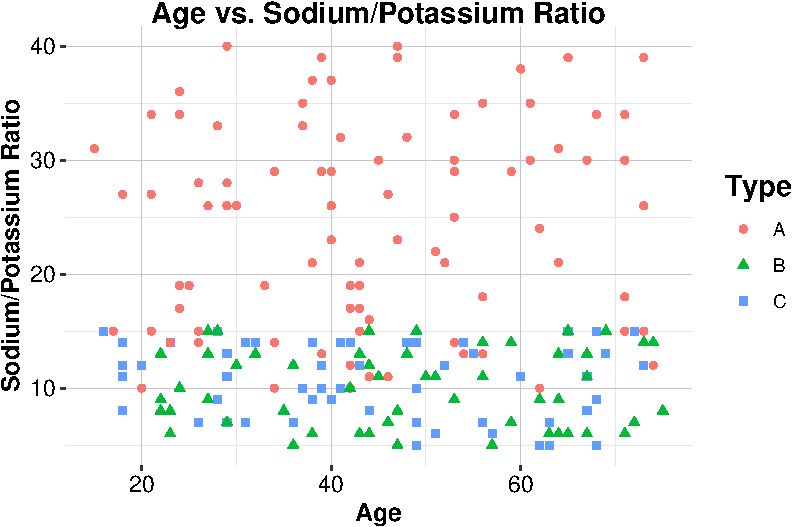
\includegraphics[width=0.65\linewidth,height=\textheight,keepaspectratio]{1-Intro-R_files/figure-pdf/unnamed-chunk-69-1.pdf}
\end{center}

\begin{enumerate}
\def\labelenumi{\arabic{enumi}.}
\setcounter{enumi}{18}
\tightlist
\item
  Add an \texttt{Outcome} variable to \texttt{drug\_data} where:
\end{enumerate}

\begin{itemize}
\tightlist
\item
  \texttt{Type\ ==\ "A"} has a high chance of \texttt{"Good"} outcome,
\item
  \texttt{Type\ ==\ "B"} or \texttt{"C"} have a lower chance of
  \texttt{"Good"}.
\end{itemize}

\begin{enumerate}
\def\labelenumi{\arabic{enumi}.}
\setcounter{enumi}{19}
\item
  Create a scatter plot of \texttt{Age} vs.~\texttt{Ratio}, colored by
  \texttt{Outcome}.
\item
  Create an \texttt{Age\_group} variable:
\end{enumerate}

\begin{itemize}
\tightlist
\item
  \texttt{"Young"} if age \(\leq\) 30,
\item
  \texttt{"Middle-aged"} if 31 \(\leq\) age \(\leq\) 50,
\item
  \texttt{"Senior"} if age \(>\) 50.
\end{itemize}

\begin{enumerate}
\def\labelenumi{\arabic{enumi}.}
\setcounter{enumi}{21}
\tightlist
\item
  Calculate the mean \texttt{Ratio} for each \texttt{Age\_group}.
\item
  Use \textbf{ggplot2} to create a bar chart showing average
  \texttt{Ratio} by \texttt{Age\_group}.
\item
  Create a new variable \texttt{Risk\_factor\ =\ Ratio\ *\ Age\ /\ 10}.
  Summarize how \texttt{Risk\_factor} differs by \texttt{Type}.
\item
  Visualize \texttt{Risk\_factor} in two ways:
\end{enumerate}

\begin{itemize}
\tightlist
\item
  A histogram grouped by \texttt{Type}.
\item
  A boxplot grouped by \texttt{Outcome}.
\end{itemize}

\begin{enumerate}
\def\labelenumi{\arabic{enumi}.}
\setcounter{enumi}{25}
\tightlist
\item
  Use R and \textbf{ggplot2} to recreate Figure
  \ref{fig-ch1-tiny-gains}, which illustrates the compounding effect of
  small improvements. First, generate a data frame with three curves:
\end{enumerate}

\begin{itemize}
\tightlist
\item
  \(y = (1.01)^x\) (\(1%
  \) better each day),
\item
  \(y = (0.99)^x\) (\(1%
  \) worse each day),
\item
  \(y = 1\) (no change).
\end{itemize}

Then use \texttt{geom\_line()} to plot the curves. Customize line colors
and add informative labels using \texttt{annotate()}. \emph{Hint:} Refer
to the example in Section \ref{sec-ch1-visualization}.

\begin{enumerate}
\def\labelenumi{\arabic{enumi}.}
\setcounter{enumi}{26}
\tightlist
\item
  Extend the Tiny Gains plot created in Exercise 26 by:
\end{enumerate}

\begin{itemize}
\tightlist
\item
  Changing the x-axis label to \texttt{"Days\ of\ Practice"},
\item
  Applying a theme such as \texttt{theme\_minimal()},
\item
  Adding a title: \texttt{"The\ Power\ of\ Consistent\ Practice"},
\item
  Saving the plot using \texttt{ggsave()} as a PDF or PNG file.
\end{itemize}

\begin{enumerate}
\def\labelenumi{\arabic{enumi}.}
\setcounter{enumi}{27}
\tightlist
\item
  For Exercise 26, change the number of days in your tiny gains plot.
  What do you observe if you compare 30 days to 365?
\end{enumerate}

\subsubsection*{Reflect and Connect}\label{reflect-and-connect}
\addcontentsline{toc}{subsubsection}{Reflect and Connect}

These reflection questions encourage you to pause, assess your progress,
and consider your goals as you continue.

\begin{enumerate}
\def\labelenumi{\arabic{enumi}.}
\setcounter{enumi}{28}
\item
  Which concepts in this chapter felt most intuitive, and which ones did
  you find challenging?
\item
  How might these skills help you analyze data in your own research or
  field of study?
\item
  Looking ahead, what would you like to be able to do with R by the end
  of this book?
\end{enumerate}

\bookmarksetup{startatroot}

\chapter{Foundations of Data Science and Machine
Learning}\label{sec-ch2-intro-data-science}

How does Netflix know what you want to watch, or how can a hospital
predict patient risk before symptoms appear? Behind these intelligent
systems lies the power of \emph{data science} and \emph{machine
learning}. This chapter offers your entry point into that world, even if
you have never written a line of code or studied statistics before.

Whether your background is in business, science, the humanities, or none
of the above, this chapter is designed to be both accessible and
practical. Through real-world examples, visual explanations, and
hands-on exercises, you will explore how data science projects progress
from raw data to meaningful insights, understand where machine learning
fits in, and see why these tools are essential in today's data-driven
world.

\emph{Data science} is a fast-moving, interdisciplinary field that
integrates computational, statistical, and analytical techniques to
extract insights from data. In today's economy, data has become one of
the world's most valuable assets, often referred to as the \emph{``new
oil''}, for its power to fuel innovation and transform decision-making.

Data science unleashes this potential by turning raw information into
actionable knowledge. It draws on machine learning, programming,
statistical modeling, and domain expertise to help organizations make
evidence-based decisions, improve operations, anticipate trends, and
build adaptive, intelligent systems. These capabilities are already
transforming industries, including personalized healthcare and financial
forecasting to targeted marketing and autonomous vehicles.

As the demand for data-driven solutions continues to grow, understanding
the foundations of data science, and its deep connection to machine
learning, has never been more important. This chapter introduces the
core concepts, explores their societal relevance, and presents a
structured workflow that guides data science projects from raw data to
real impact.

While data science encompasses a wide variety of data types, including
images, video, audio, and text, this book focuses on applications
involving \emph{structured, tabular data}. These are datasets commonly
found in spreadsheets, relational databases, and logs. More complex
forms of unstructured data analysis, such as computer vision or natural
language processing, lie beyond the scope of this volume.

\subsection*{What This Chapter Covers}\label{what-this-chapter-covers-1}
\addcontentsline{toc}{subsection}{What This Chapter Covers}

This chapter lays the groundwork for your journey into data science and
machine learning. You will start by exploring what data science is, why
it matters across diverse fields, and how it transforms raw data into
real-world impact. You will then learn how data science projects are
structured using a practical workflow that guides you from defining the
problem to deploying a solution.

As the chapter progresses, you will gain insight into the role of
machine learning as the modeling engine of data science. We break down
its three main branches, supervised, unsupervised, and reinforcement
learning, highlighting how they differ and where each is applied.

By the end of this chapter, you will have a high-level roadmap of how
data science works in practice, what kinds of problems it can solve, and
how the rest of this book will help you build and evaluate machine
learning models with confidence. While this chapter offers a broad
overview, the detailed methods, tools, and techniques will be introduced
progressively in the chapters that follow.

\section{What is Data Science?}\label{what-is-data-science}

Data science is an interdisciplinary field that combines mathematics,
statistics, computer science, and domain knowledge to uncover patterns
and generate actionable insights (see Figure \ref{fig-Data-Science}). It
integrates analytical methods and machine learning to process large,
complex datasets and support informed decision-making, strategic
planning, and innovation.

\begin{figure}[H]

\centering{

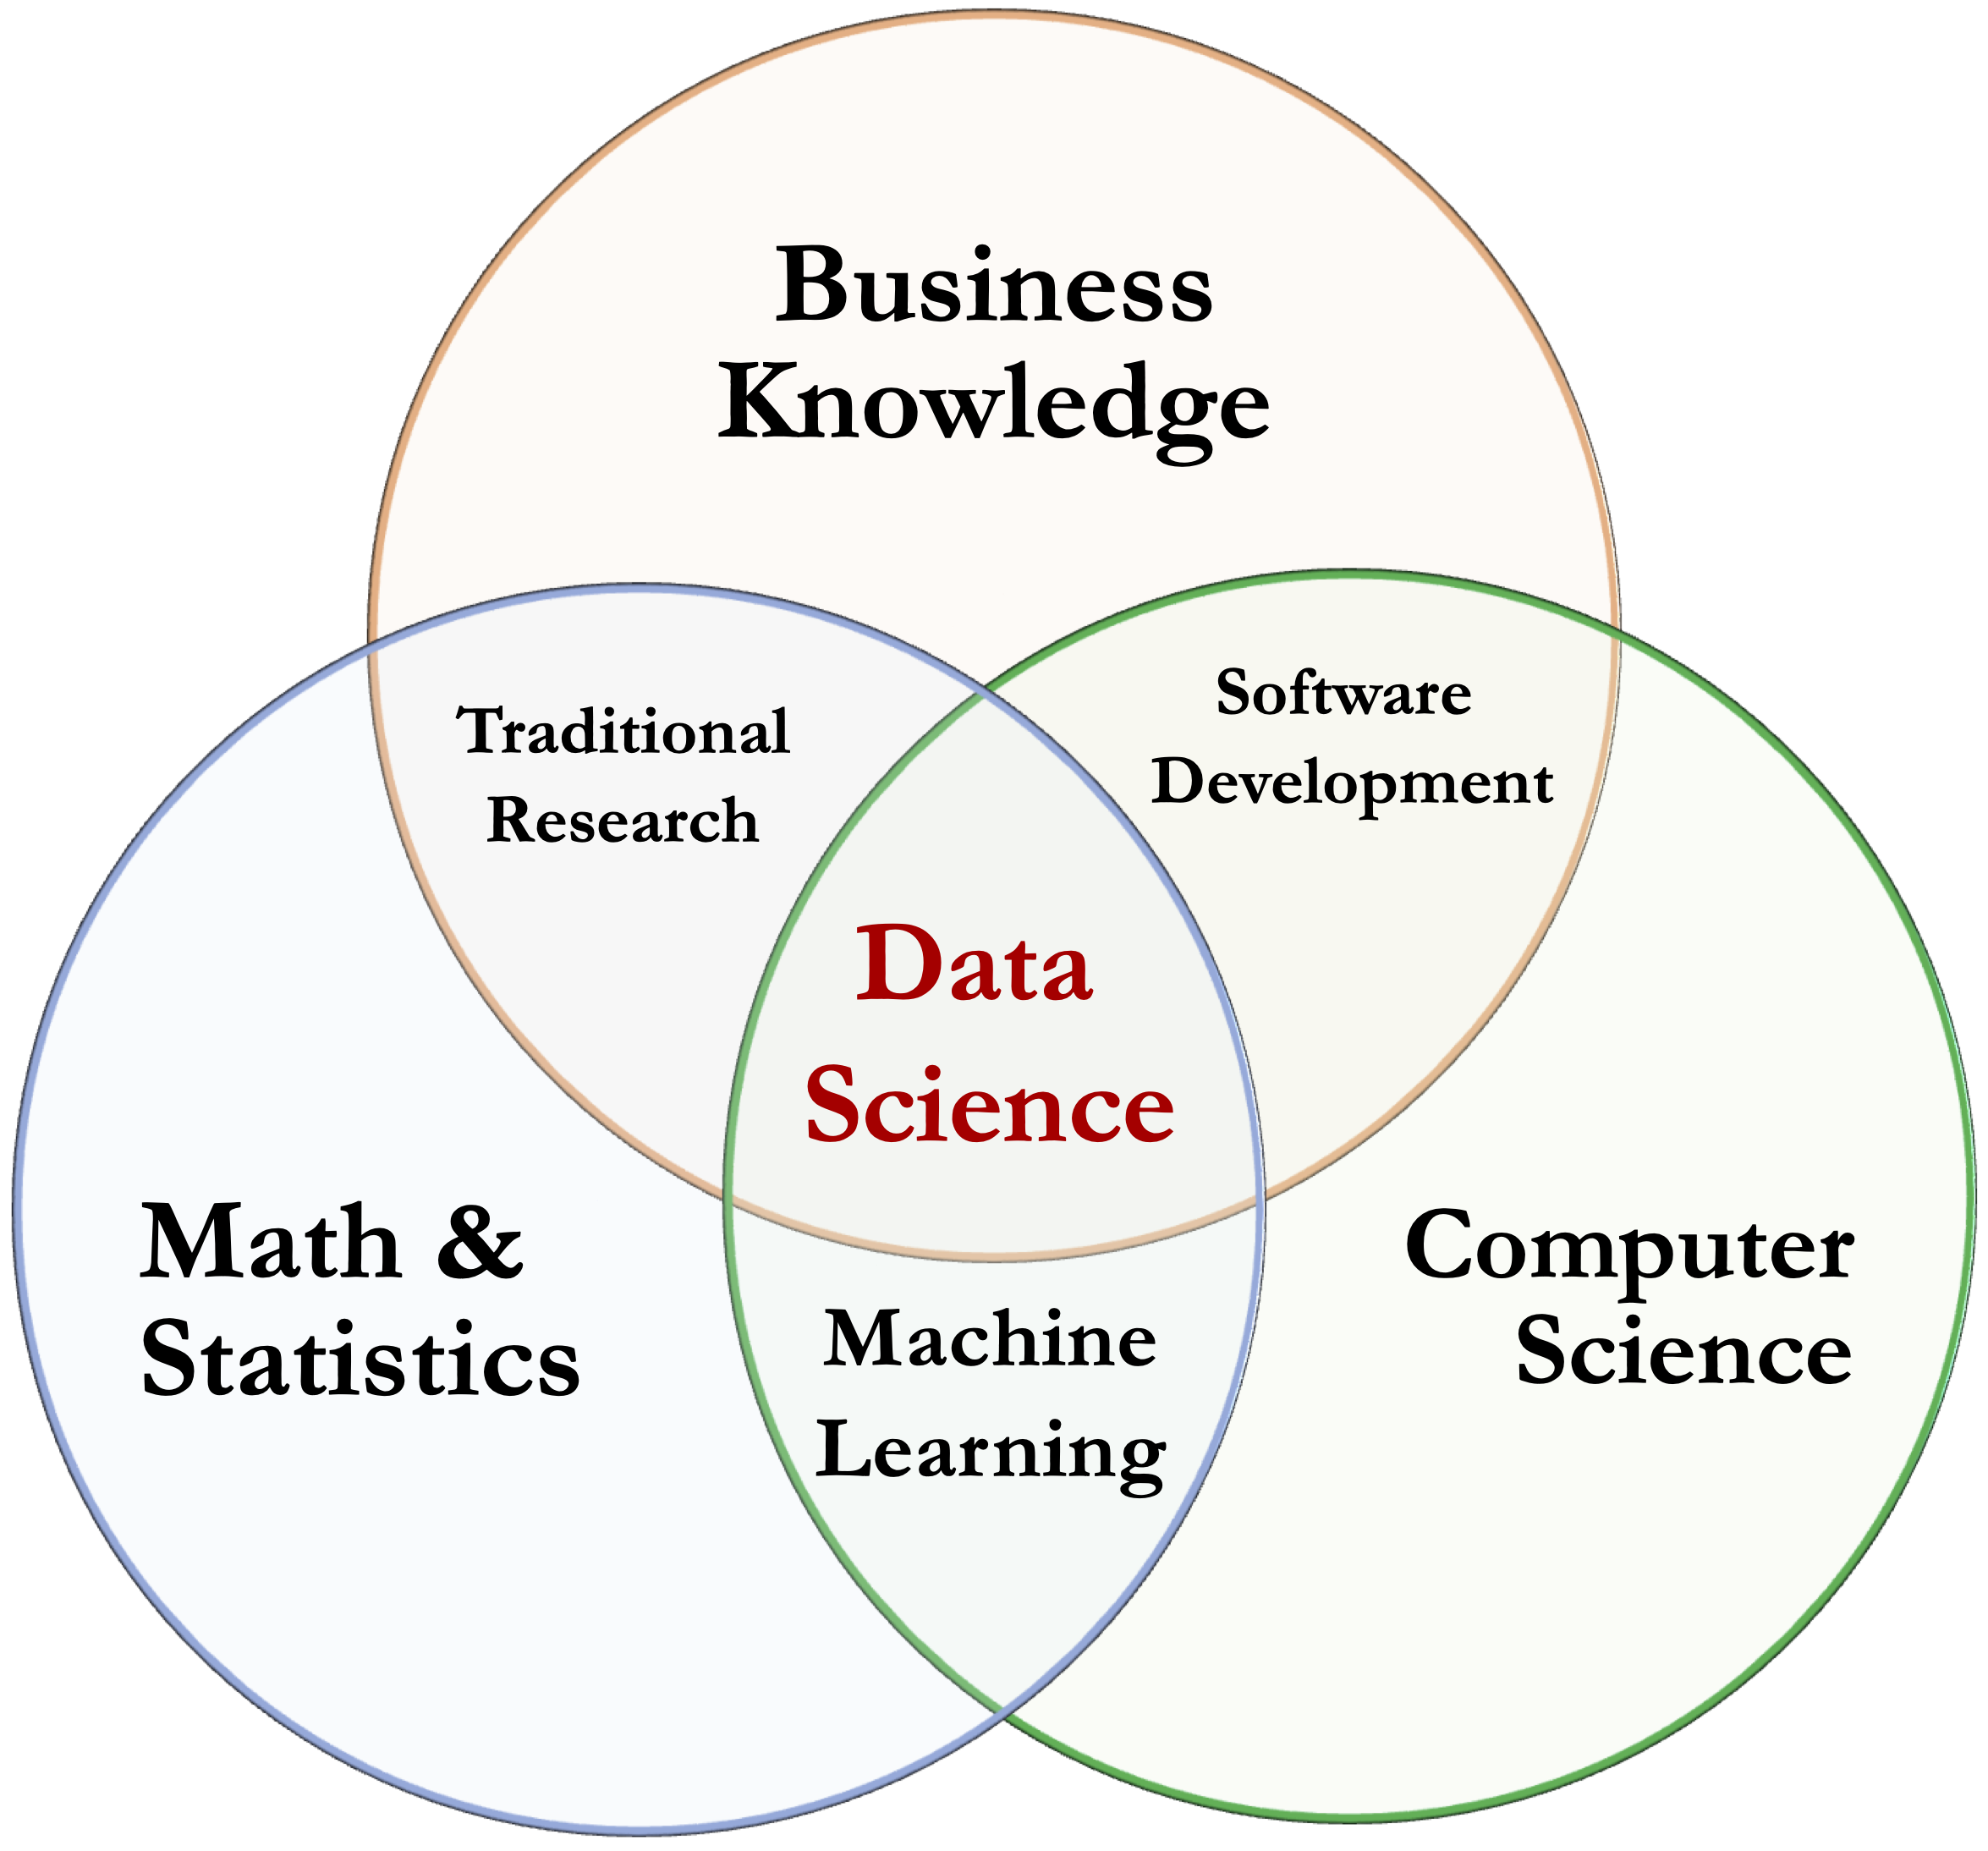
\includegraphics[width=0.4\linewidth,height=\textheight,keepaspectratio]{images/ch2_data_science.png}

}

\caption{\label{fig-Data-Science}Venn diagram of data science (inspired
by Drew Conway's original illustration). Data science is a
multidisciplinary field that integrates computational skills,
statistical reasoning, and domain knowledge to extract insights from
data.}

\end{figure}%

Although the term \emph{data science} is relatively new, its foundations
are rooted in long-established disciplines such as statistics, data
analysis, and machine learning. What distinguishes modern data science
is its scale and impact: the explosion of digital data, increasing
computational resources, and the growing demand for intelligent systems
have transformed it into a distinct and essential field.

At its core is \emph{machine learning}, the study of algorithms that
learn from data and improve their performance through experience. While
statistical methods help summarize and infer from data, machine learning
provides scalable approaches to discover complex patterns, automate
predictions, and build adaptive systems. In this way, machine learning
is not just a component of data science; it is one of its principal
engines.

In practice, data science involves framing questions, analyzing data,
developing models, and translating results into meaningful action. It
draws on tools such as data visualization, predictive modeling, and
domain-specific techniques to help organizations derive value from the
information they generate and collect.

\subsection*{Key Components of Data
Science}\label{key-components-of-data-science}
\addcontentsline{toc}{subsection}{Key Components of Data Science}

Modern data science integrates three core components that work together
to transform data into insight and enable intelligent systems:

\begin{itemize}
\item
  \emph{Data engineering} Focuses on the collection, storage, and
  organization of data. This includes building data pipelines and
  infrastructure that ensure data is reliable, scalable, and accessible.
  This book introduces essential techniques for data cleaning and
  preparation in Chapters \ref{sec-ch3-data-preparation} and
  \ref{sec-ch6-setup-data}. More advanced topics, such as distributed
  systems and real-time data processing, are beyond the scope of this
  volume. For further reading, see
  \href{https://mdsr-book.github.io/mdsr3e}{Modern Data Science with R}
  (2017).
\item
  \emph{Statistical analysis and data visualization} These methods
  support both exploration and inference. They help uncover patterns,
  test hypotheses, and guide decisions throughout the modeling process.
  From visualizing trends to quantifying uncertainty, statistical
  thinking is essential for interpreting and communicating data. We
  focus on these skills in Chapters \ref{sec-ch4-EDA} and
  \ref{sec-ch5-statistics}.
\item
  \emph{Machine learning} Enables algorithms to automatically learn
  patterns, make predictions, and adapt to new information. Techniques
  range from supervised learning to deep neural networks, and are
  introduced progressively in Chapters \ref{sec-ch7-classification-knn}
  through \ref{sec-ch13-clustering}.
\end{itemize}

These components are developed step by step throughout the book,
starting with data preparation and exploratory analysis and culminating
in model building, evaluation, and deployment. Together, they provide
the foundation for effective and reproducible data science practice.

\section{Why Data Science Matters}\label{why-data-science-matters}

Data is no longer just a byproduct of digital systems; it has become a
core asset for innovation, strategy, and decision-making. Today's most
influential organizations, including OpenAI, Google, Apple, and Amazon,
demonstrate how data, when combined with algorithms and computing power,
can personalize products, optimize operations, and reshape entire
industries.

In nearly every domain, data-driven decision-making is now essential.
Organizations collect vast amounts of information every day, from sales
transactions and web activity to clinical trials and financial records.
Without the right tools and expertise, much of this data remains
underutilized. Data science helps bridge this gap by identifying
patterns, generating predictions, and delivering insights that support
more adaptive, evidence-based decisions.

Data science influences a wide range of sectors, including finance,
where it is used for credit scoring, fraud detection, algorithmic
trading, and regulatory compliance; marketing, where it enables audience
segmentation and campaign optimization based on behavioral data; retail
and e-commerce, where it supports inventory forecasting, dynamic
pricing, and product recommendation systems; and healthcare, where it
assists in early diagnosis, risk stratification, and personalized
treatment planning.

Common technologies highlight these capabilities: Netflix recommends
content based on viewing history, Amazon forecasts purchasing needs, and
navigation systems dynamically reroute traffic. Such tools are built on
structured historical data, statistical modeling, and iterative
refinement.

To build systems like these, data scientists rely on a structured,
repeatable approach. In the next section, we introduce the \emph{data
science workflow}, a practical framework that guides projects from
initial questions to actionable insights.

\section{The Data Science Workflow}\label{the-data-science-workflow}

Have you ever tried solving a complex problem, like diagnosing a
patient, optimizing a delivery route, or designing a product, without a
plan? In data science, structure is everything. Without it, even the
most powerful algorithms can lead to misleading or irrelevant results.

That is why data science relies on a clear, organized workflow. The
\emph{data science workflow} provides a flexible yet disciplined
approach to transforming messy data into actionable insights. It helps
teams align their efforts, iterate thoughtfully, and ensure that results
are accurate, reproducible, and useful.

This process is not linear---it is \emph{iterative}. As you gain new
insights, you often revisit earlier steps: redefining questions,
adjusting features, or retraining models. This cyclical nature is what
makes data science dynamic and adaptive.

A helpful way to visualize this transformation is through the \emph{DIKW
Pyramid}, which illustrates how raw \emph{Data} becomes
\emph{Information}, then \emph{Knowledge}, and finally \emph{Wisdom}
(see Figure \ref{fig-DIKW-Pyramid}).

\begin{figure}[H]

\centering{

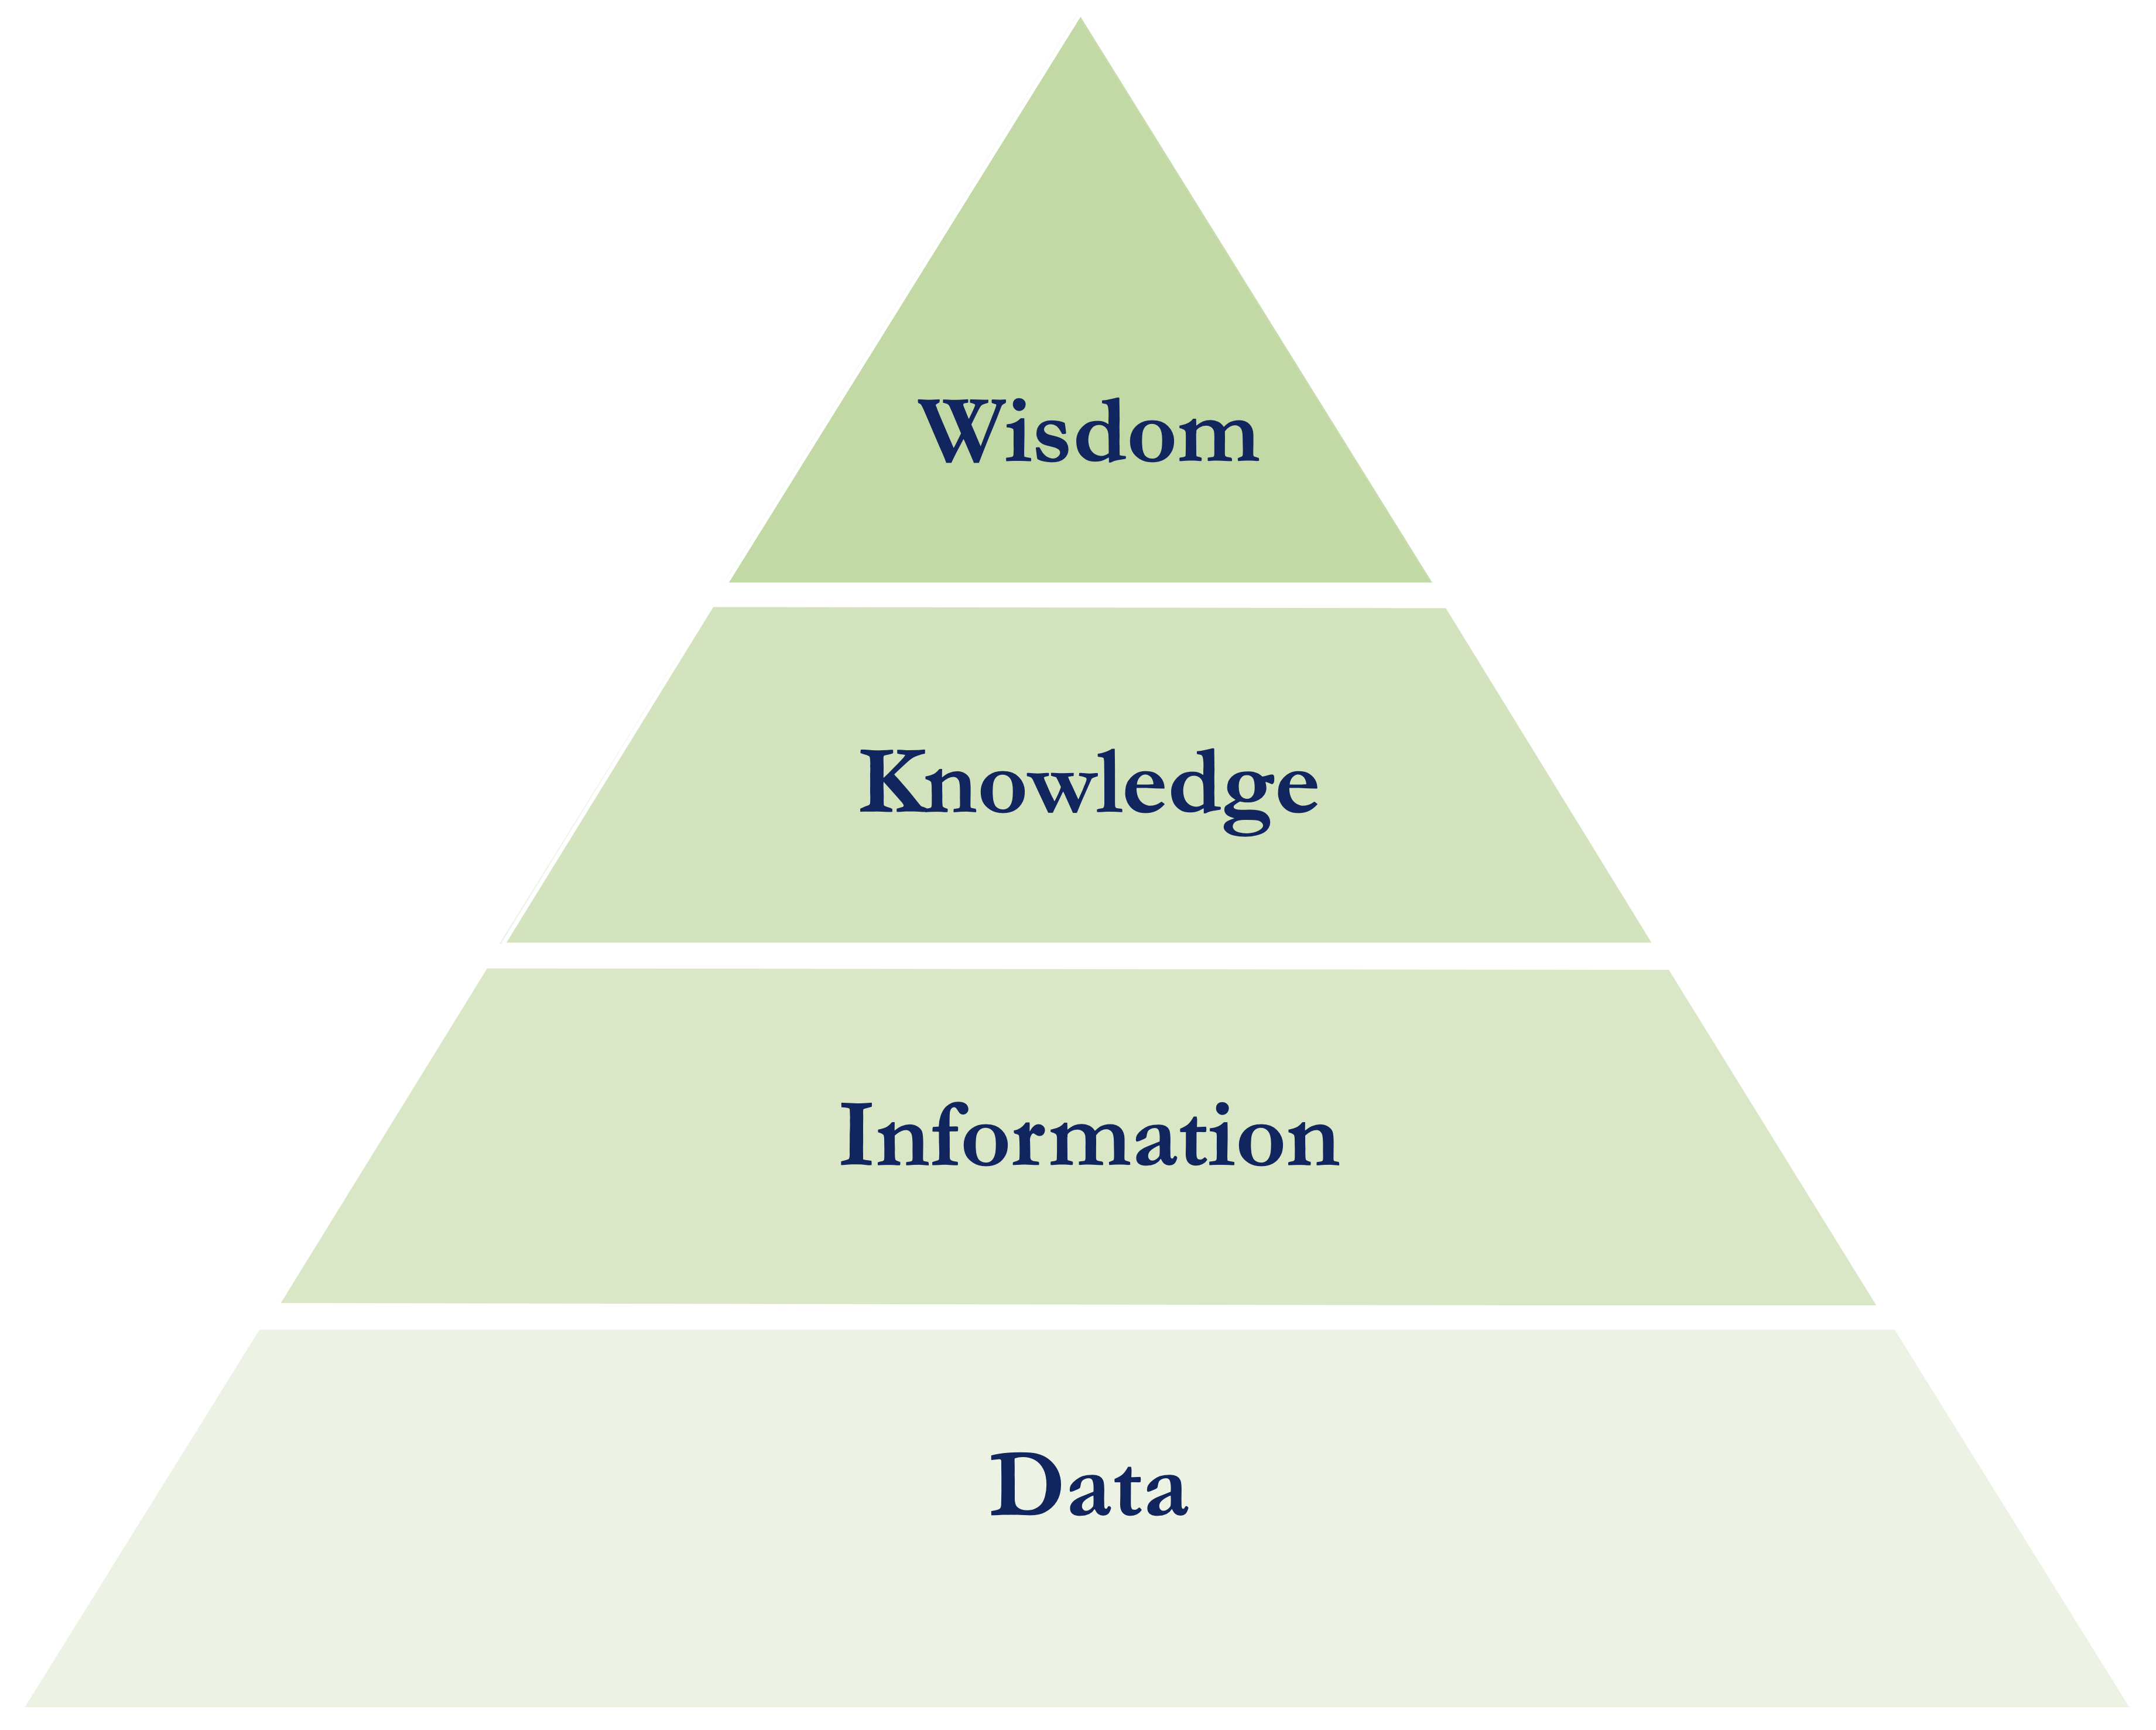
\includegraphics[width=0.45\linewidth,height=\textheight,keepaspectratio]{images/ch2_DIKW-Pyramid.png}

}

\caption{\label{fig-DIKW-Pyramid}The DIKW Pyramid illustrates the
transformation of raw data into higher-order insights, progressing from
data to information, knowledge, and ultimately wisdom.}

\end{figure}%

To put this into action, we use a practical framework called
\emph{CRISP-DM} (Cross-Industry Standard Process for Data Mining). It
guides data science projects through seven interconnected phases (see
Figure \ref{fig-ch2_DSW}):

\begin{enumerate}
\def\labelenumi{\arabic{enumi}.}
\item
  \emph{Problem Understanding} -- Define the business or research goal
  and clarify what success looks like.
\item
  \emph{Data Preparation} -- Gather, clean, and format data for
  analysis.
\item
  \emph{Exploratory Data Analysis (EDA)} -- Use summaries and
  visualizations to understand distributions, spot patterns, and
  identify potential issues.
\item
  \emph{Data Setup to Model} -- Engineer features, normalize values, and
  select predictors.
\item
  \emph{Modeling} -- Apply machine learning or statistical models to
  uncover patterns and generate predictions.
\item
  \emph{Evaluation} -- Assess how well the model performs using
  appropriate metrics and validation.
\item
  \emph{Deployment} -- Integrate the model into real-world systems and
  monitor it over time.
\end{enumerate}

\begin{figure}[H]

\centering{

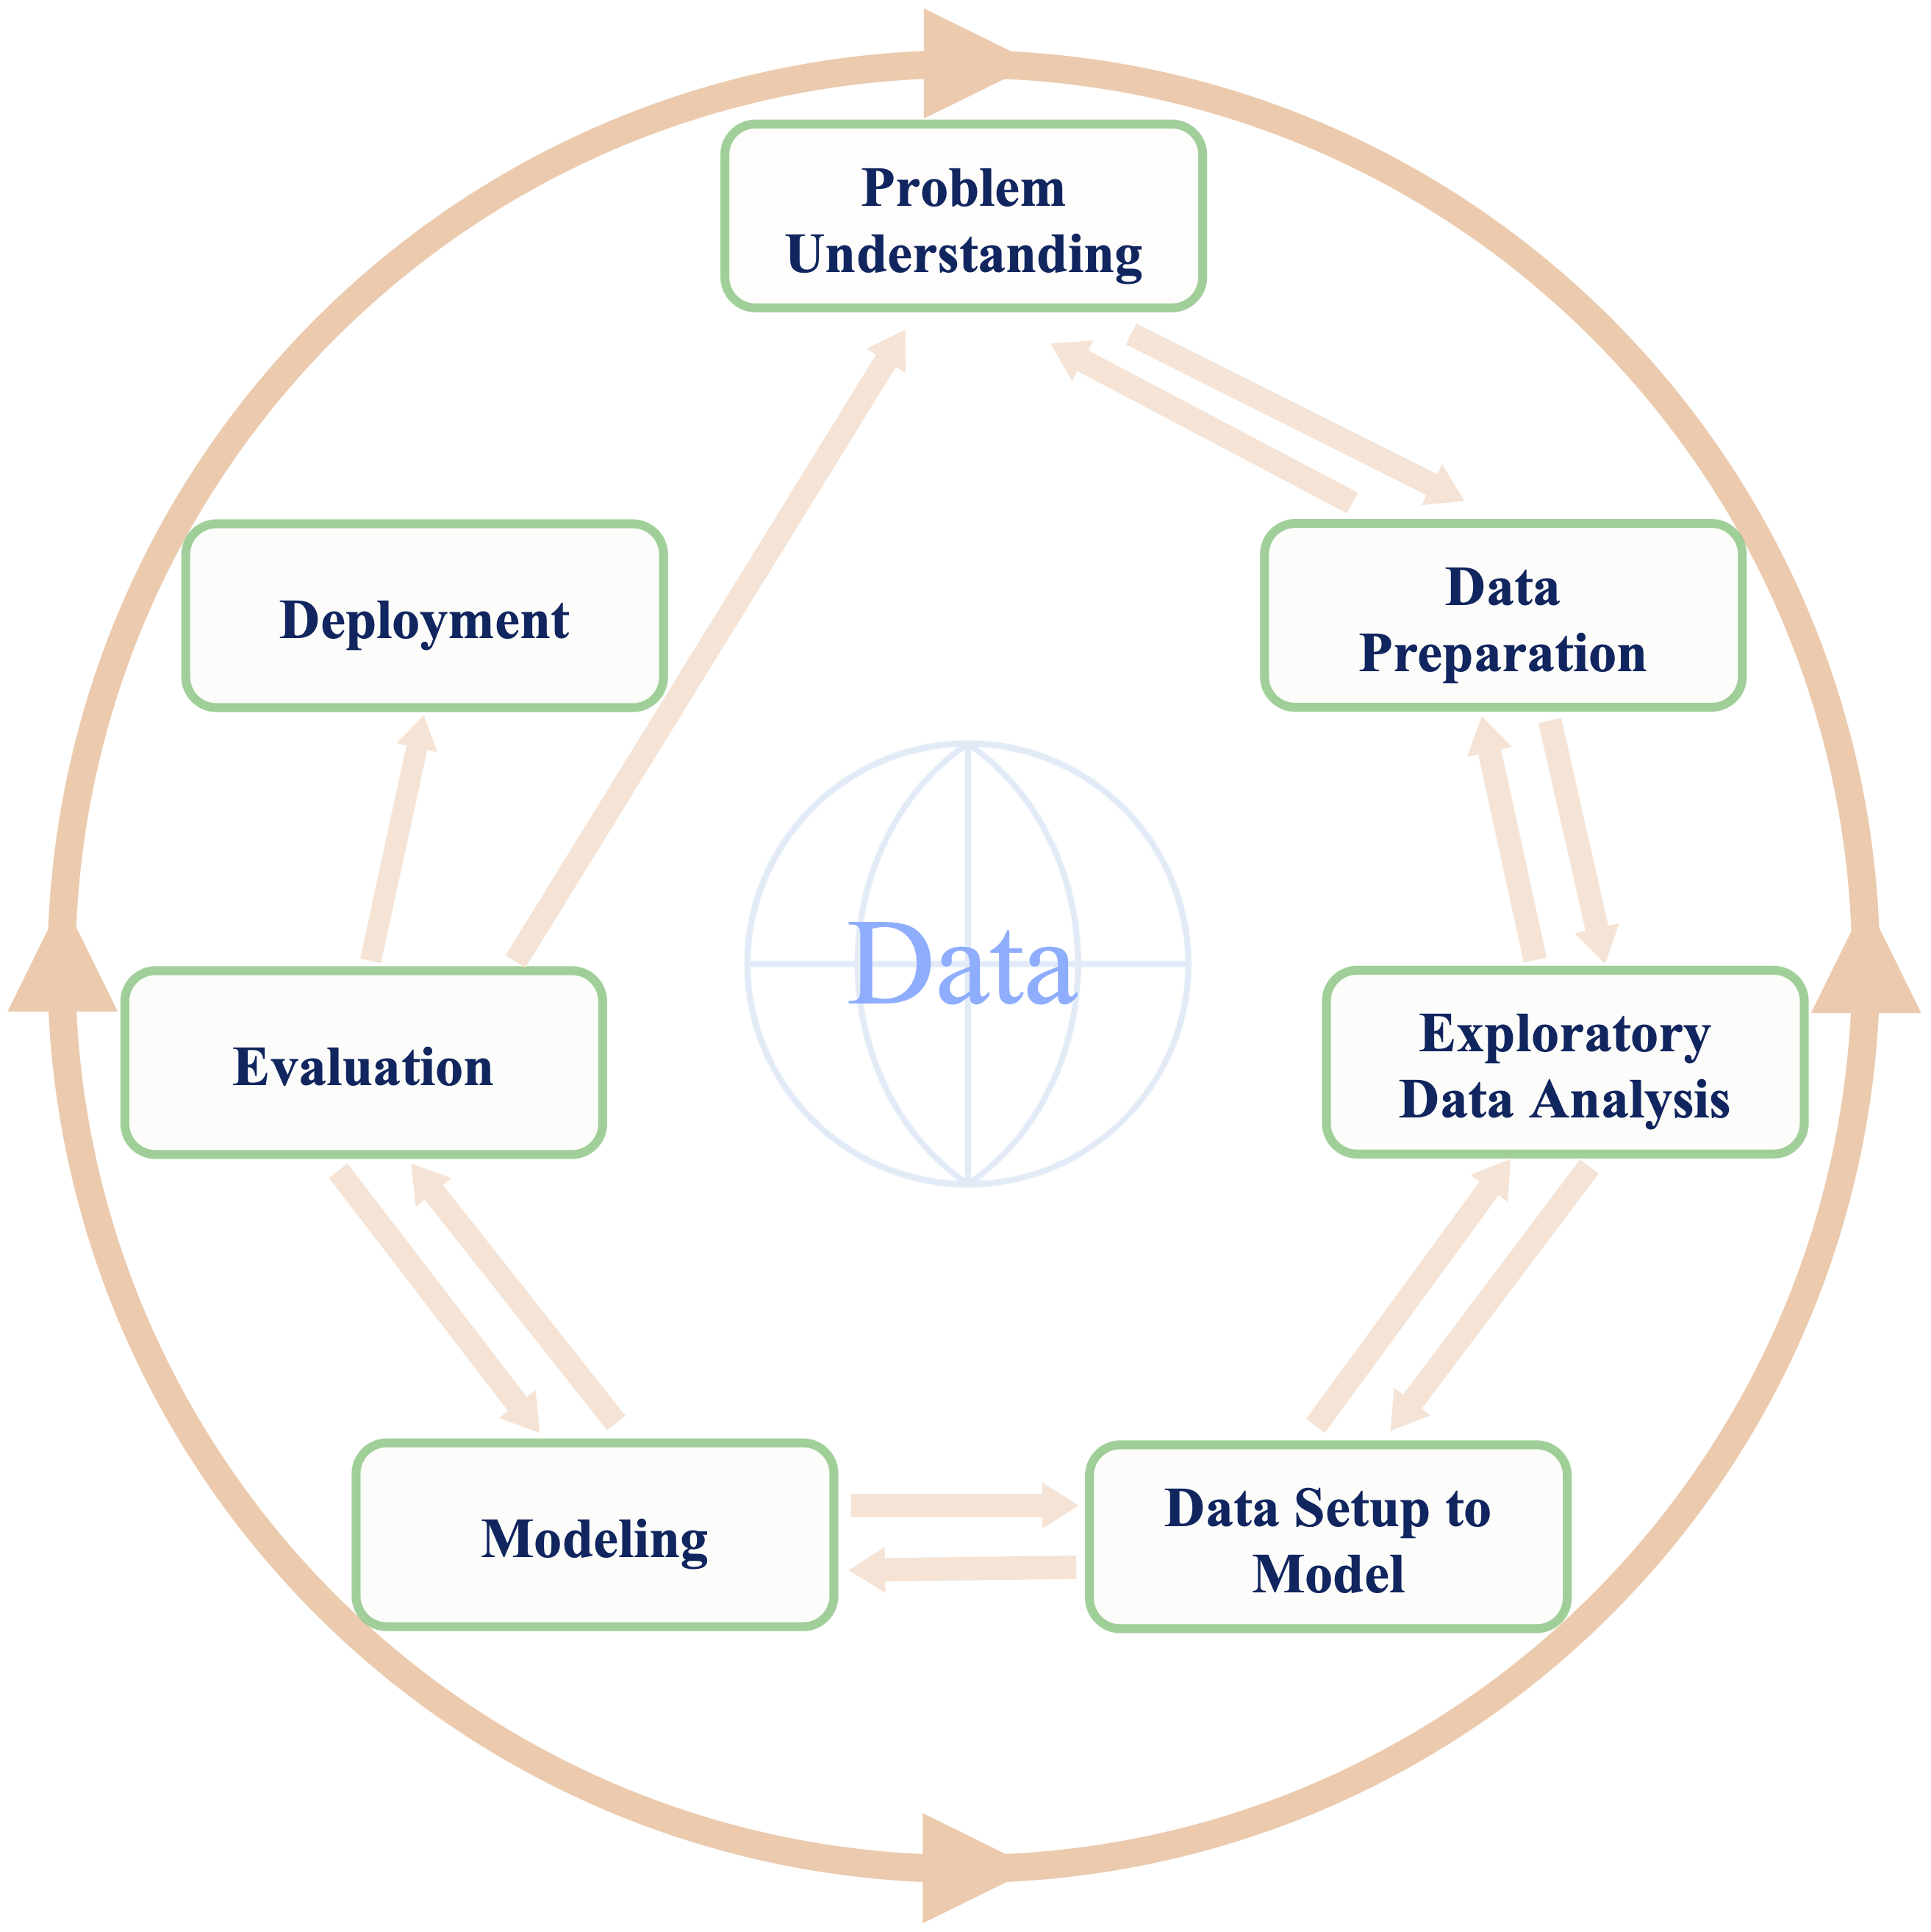
\includegraphics[width=0.75\linewidth,height=\textheight,keepaspectratio]{images/ch2_DSW.png}

}

\caption{\label{fig-ch2_DSW}The Data Science Workflow is an iterative
framework for structuring data science and machine learning projects.
Inspired by the CRISP-DM model, it emphasizes reproducibility,
continuous refinement, and impact-driven analysis.}

\end{figure}%

Because real-world data is messy, and questions evolve, this process is
rarely completed in one pass. A model that performs poorly might send
you back to feature engineering. A surprising pattern during EDA might
reshape your original question. Embracing this iterative process is key
to success in data science, and to building systems that truly make an
impact.

This book is structured around the Data Science Workflow. Each chapter
corresponds to one or more stages in this process, guiding you step by
step from problem definition to deployment. This is the same framework I
use in my courses and when supervising BSc and MSc thesis projects in
data science. By following this approach, students not only learn
individual techniques, but also develop the process-oriented mindset
essential for real-world practice.

In the remainder of this chapter, we walk through each stage of the Data
Science Workflow, starting with problem understanding and moving through
data preparation, modeling, and evaluation, illustrating how these steps
connect and why each is essential for building effective, data-driven
solutions.

\section{Problem Understanding}\label{sec-ch2-Problem-Understanding}

Every data science project begins not with code or data, but with a
clearly defined question. Whether the goal is to test a scientific
hypothesis, improve business operations, or enhance user experience,
success depends on understanding the problem clearly and aligning it
with stakeholder needs. This initial stage in the Data Science Workflow
ensures that projects address meaningful goals and lay the foundation
for actionable outcomes.

A well-known example from World War II illustrates the importance of
framing problems effectively: the case of
\href{https://en.wikipedia.org/wiki/Abraham_Wald}{Abraham Wald} and the
missing bullet holes. During the war, the U.S. military analyzed
returning aircraft to determine which areas were most damaged. Bullet
holes appeared mostly on the fuselage and wings, but few were found in
the engines. Figure \ref{fig-case-WW2-plane} illustrates this pattern,
summarized in Table \ref{tbl-WW2-bullet-holes}.

\begin{figure}[H]

\centering{

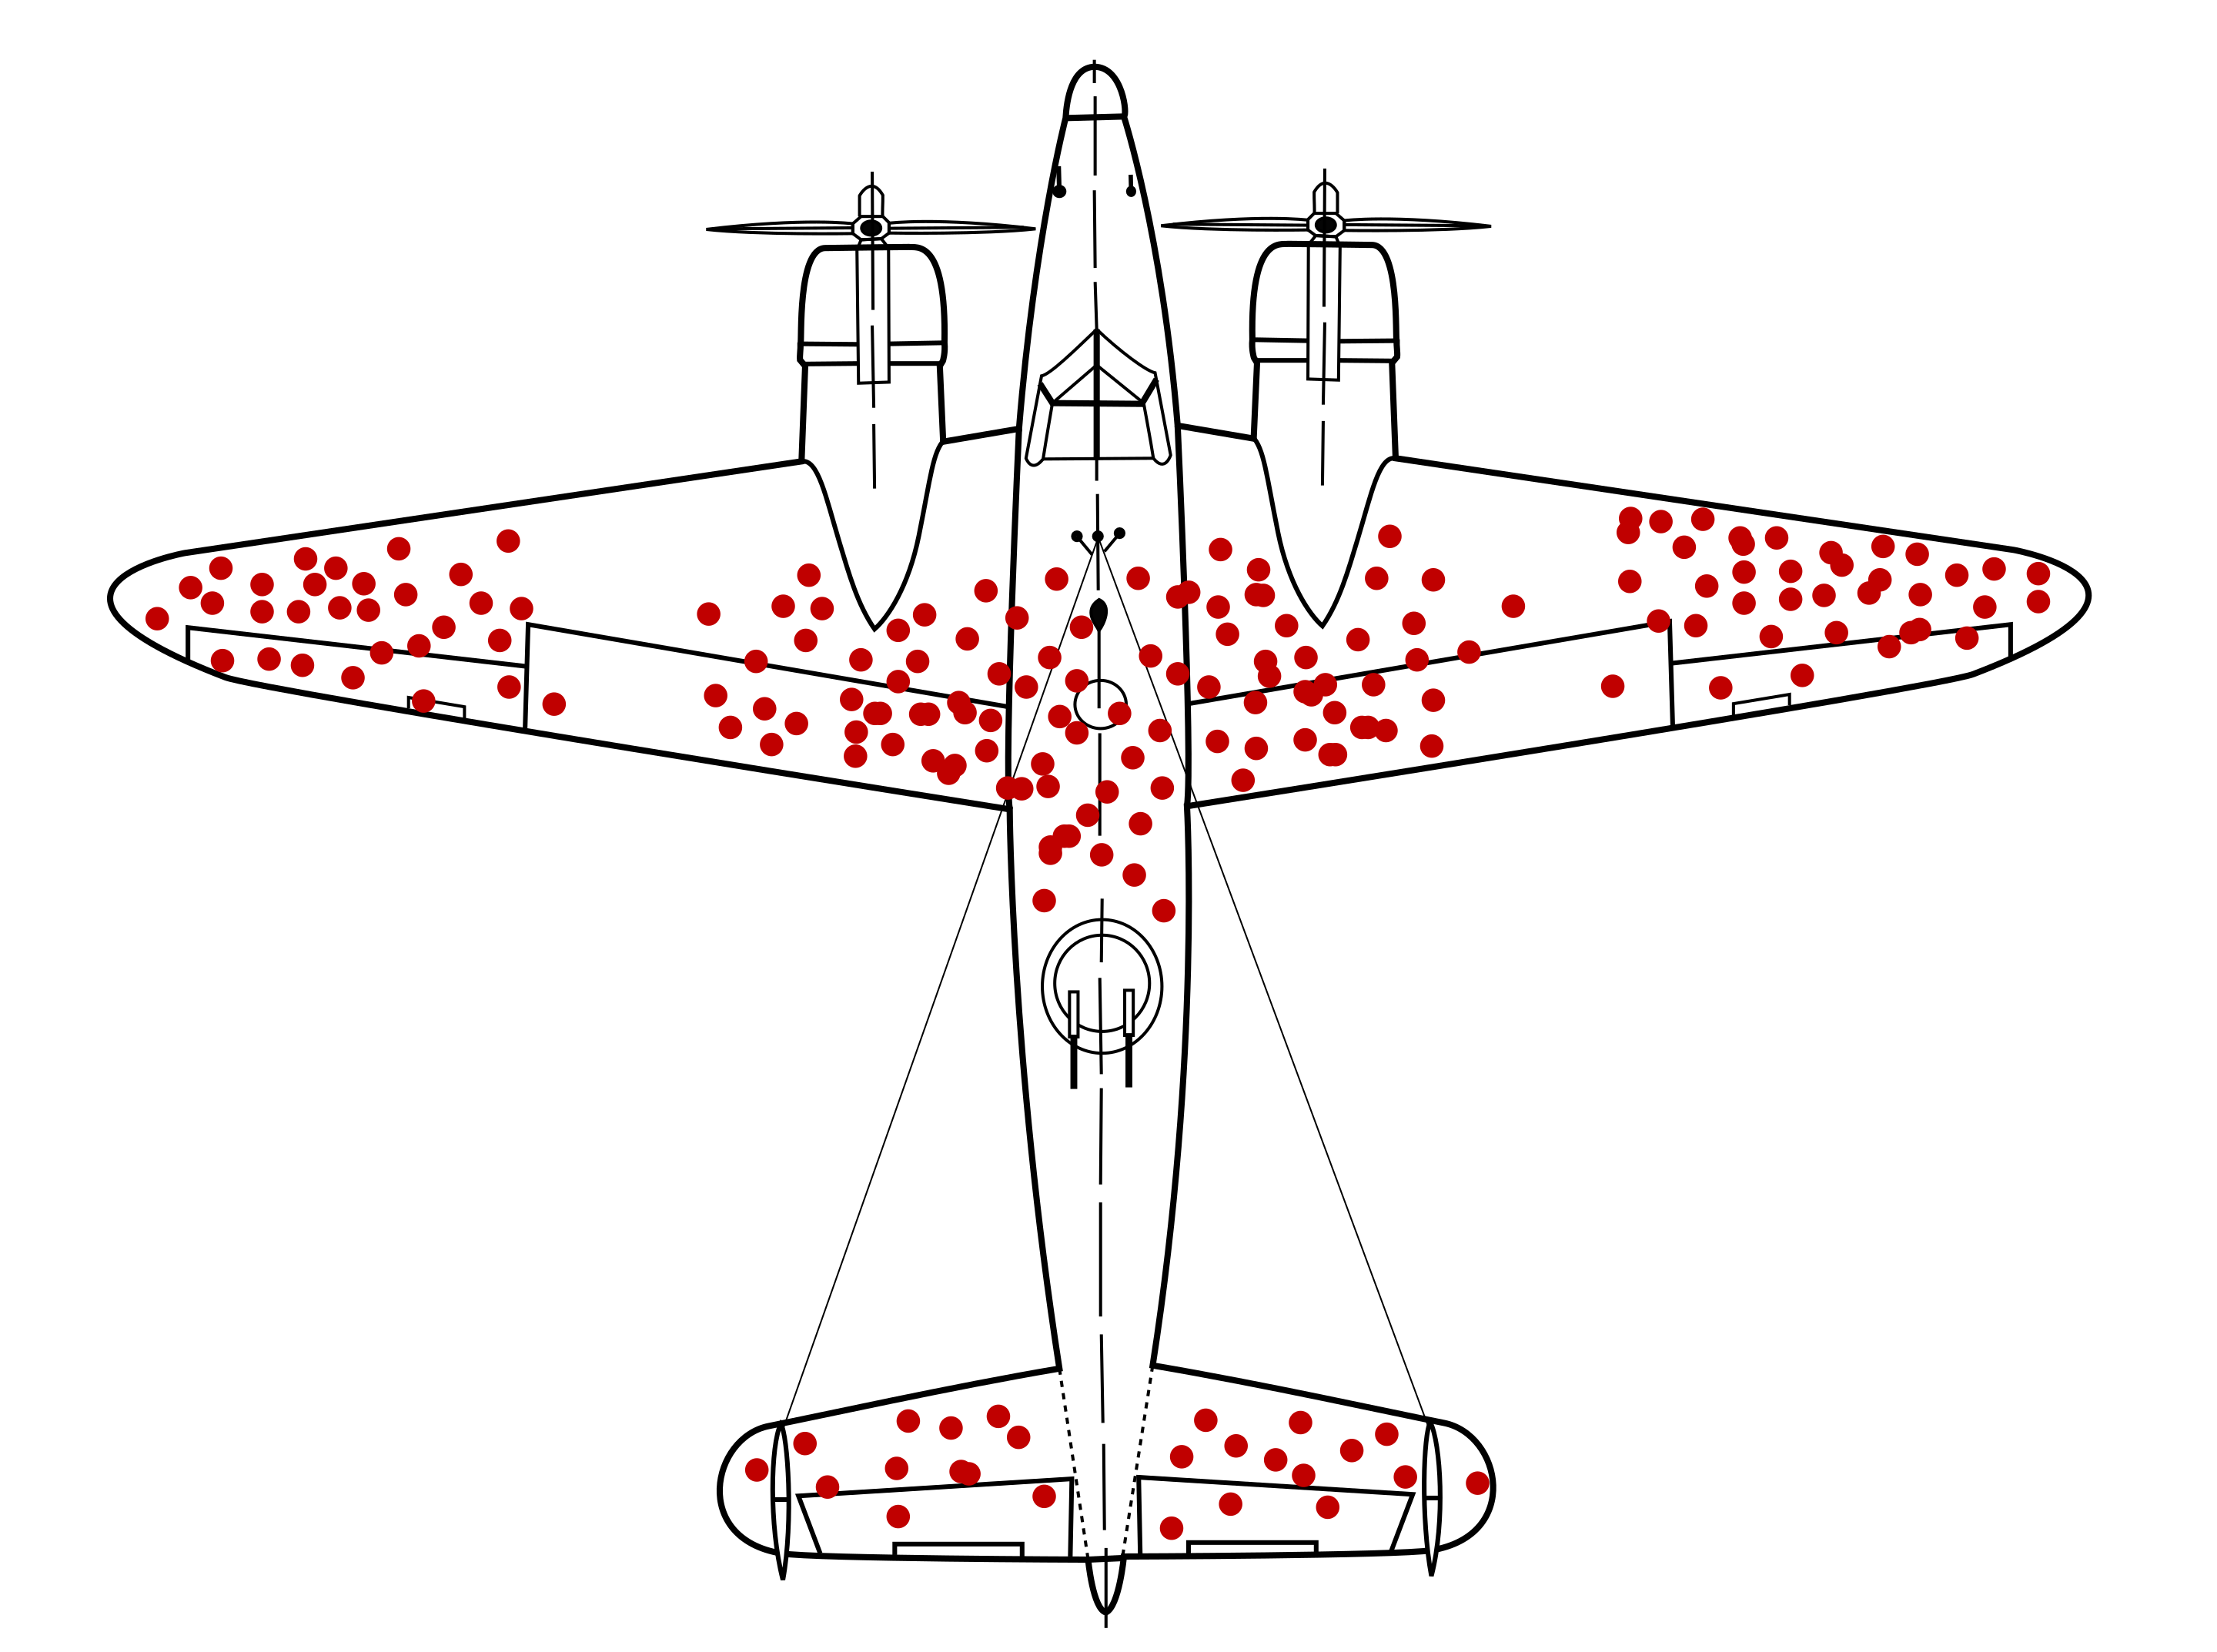
\includegraphics[width=0.45\linewidth,height=\textheight,keepaspectratio]{images/ch2_case_WW2_plane.png}

}

\caption{\label{fig-case-WW2-plane}Bullet damage was recorded on planes
that returned from missions. Those hit in more vulnerable areas did not
return. (Image: Wikipedia).}

\end{figure}%

\begin{table}

\caption{\label{tbl-WW2-bullet-holes}Distribution of bullet holes per
square foot on returned aircraft.}

\centering{

\centering
\begin{tabular}[t]{>{}l>{\raggedleft\arraybackslash}p{15em}}
\toprule
Section.of.plane & Bullet.holes.per.square.foot\\
\midrule
\textcolor{black}{\textbf{Engine}} & 1.11\\
\textcolor{black}{\textbf{Fuselage}} & 1.73\\
\textcolor{black}{\textbf{Fuel system}} & 1.55\\
\textcolor{black}{\textbf{Rest of plane}} & 0.31\\
\bottomrule
\end{tabular}

}

\end{table}%

Initial recommendations focused on reinforcing the most damaged areas.
But statistician Abraham Wald came to a different conclusion: the data
reflected only the planes that survived. The engines, where little
damage was observed, were likely the areas where hits caused planes to
be lost. His counterintuitive insight was to reinforce the areas with no
bullet holes.

This story highlights a central principle in data science: the most
valuable insights may lie in what is missing, unseen, or misinterpreted.
Without careful problem framing, even high-quality data can lead to
flawed conclusions.

While platforms such as \href{https://www.kaggle.com}{Kaggle} often
begin with clearly posed questions and pre-processed datasets,
real-world data science rarely starts that way. In practice, analysts
must begin with the first step in the Data Science Workflow: working
with stakeholders to define objectives and determine how data can be
used to address them. This ability to frame problems thoughtfully is one
of the most important skills for a data scientist. The datasets used in
this book, such as those in the \textbf{liver} package, are also
pre-cleaned to support focused learning. But real-world projects often
involve vague goals and messy data, making the problem formulation stage
even more critical.

This phase involves close collaboration with business leaders,
researchers, or domain experts to clarify objectives, define success
criteria, and understand key constraints. Helpful questions include:

\begin{itemize}
\item
  \emph{Why} is this question important?
\item
  \emph{What} outcome or impact is desired?
\item
  \emph{How} can data science contribute meaningfully?
\end{itemize}

As Simon Sinek emphasizes in his TED talk
\href{https://www.ted.com/talks/simon_sinek_how_great_leaders_inspire_action}{``How
Great Leaders Inspire Action''}, effective efforts begin by asking
\emph{why}. In data science, understanding the deeper purpose behind a
project leads to sharper analysis, better communication, and more
relevant results.

For example, building a model to ``predict churn'' only becomes valuable
when linked to a concrete goal, such as designing retention campaigns or
estimating revenue loss. The way the problem is framed shapes what data
is collected, which models are suitable, and how outcomes are evaluated.

Once the problem is well understood, the next step is connecting it to
data. This translation is rarely straightforward and often requires both
domain expertise and creative thinking. A technically correct model may
still fall short if the underlying question is poorly formulated. To
turn business or research goals into effective data science tasks, the
following structured approach can be useful:

\begin{enumerate}
\def\labelenumi{\arabic{enumi}.}
\item
  \emph{Clearly articulate the project objectives} and requirements in
  terms of the overall goals of the business or research entity.
\item
  \emph{Break down the objectives} to outline specific expectations and
  desired outcomes.
\item
  \emph{Translate these objectives into a data science problem} that can
  be addressed using analytical techniques.
\item
  \emph{Draft a preliminary strategy} for how to achieve these
  objectives, considering potential approaches and methodologies.
\end{enumerate}

A well-scoped, data-aligned problem sets the stage for meaningful
analysis. The next step is preparing the data to support that goal.

\section{Data Preparation}\label{data-preparation}

With a clear understanding of the problem and its connection to data, we
can now turn to preparing the dataset for analysis. This stage ensures
that the data is accurate, consistent, and structured in a way that
supports meaningful exploration and modeling.

In practice, raw data, whether collected from databases, spreadsheets,
APIs, or web scraping, often contains issues such as missing values,
outliers, duplicates, and incompatible variable types. If unaddressed,
these issues can distort summaries, mislead models, or obscure important
relationships.

This book focuses on structured, tabular data, the kind stored in
spreadsheets, relational databases, and logs. While data science
techniques also extend to unstructured sources such as images, audio, or
text, those areas are beyond our scope here.

Typical tasks in data preparation include:

\begin{itemize}
\item
  Data collection and integration: Merging data from different sources,
  resolving schema mismatches, and aligning identifiers and time
  intervals.
\item
  Handling missing values: Addressing gaps through deletion, imputation,
  or indicator variables that flag missingness.
\item
  Outlier detection: Identifying unusual or extreme values that may
  represent input errors or highlight noteworthy patterns.
\item
  Resolving inconsistencies: Standardizing formats, correcting typos,
  and consolidating duplicated categories.
\item
  Feature engineering: Transforming or creating variables to improve
  interpretability or model performance.
\item
  Data inspection and summarization: Verifying variable types, examining
  distributions, and checking for structural issues such as duplicate
  rows, mismatched keys, or inconsistent definitions.
\end{itemize}

While often labor-intensive, careful data preparation provides the
foundation for accurate, interpretable, and reproducible analysis.
Skimping on this phase often leads to unreliable results, regardless of
the sophistication of the models that follow. In Chapter
\ref{sec-ch3-data-preparation}, we explore each of these techniques in
detail, using real-world examples to illustrate their practical
importance.

\section{Exploratory Data Analysis
(EDA)}\label{exploratory-data-analysis-eda}

Before we trust models to make predictions, we must first understand
what our data is telling us. Exploratory Data Analysis (EDA) is the
stage in the workflow where analysts examine data systematically,
developing an informed perspective on its structure, quality, and key
relationships.

EDA serves two complementary purposes. First, it plays a
\emph{diagnostic} role by revealing issues such as missing values,
outliers, or inconsistent entries that may compromise later analyses.
Second, it plays an \emph{exploratory} role by uncovering patterns and
associations that inform model building and feature engineering.

Several techniques are central to EDA:

\begin{itemize}
\item
  Summary statistics, including the mean, median, standard deviation,
  and interquartile range, provide insight into the distribution of
  numerical variables.
\item
  Visualization tools such as histograms, scatter plots, and box plots
  help reveal patterns, anomalies, and group differences.
\item
  Correlation analysis quantifies linear relationships between numeric
  variables and may suggest redundancy or predictive importance.
\end{itemize}

These tools support both data quality assessment and analytical
decision-making. For example, a skewed variable may require
transformation, or a highly correlated feature may suggest
dimensionality reduction.

In R, EDA typically begins with functions like \texttt{summary()} and
\texttt{str()} to examine structure and variable types. The
\textbf{ggplot2} package provides a versatile framework for creating
diagnostic and exploratory plots. We explore these techniques in greater
detail in Chapter \ref{sec-ch4-EDA}, using real-world datasets to
demonstrate how EDA guides effective modeling and communication.

\section{Data Setup to Model}\label{data-setup-to-model}

After gaining a clear understanding of the data through exploratory
analysis, the next step is to prepare it for modeling. This stage
bridges exploration and prediction, shaping the dataset into a form that
supports learning algorithms and ensures robust performance.

Several key tasks are typically involved:

\begin{itemize}
\item
  \emph{Feature engineering} involves creating new variables or
  transforming existing ones to better capture the information relevant
  to the modeling goal. This may include combining variables, encoding
  categorical features numerically, or applying log transformations to
  reduce skewness.
\item
  \emph{Feature selection} focuses on identifying the most informative
  predictors while removing irrelevant or redundant ones. This helps
  reduce overfitting, enhance interpretability, and improve
  computational efficiency.
\item
  \emph{Rescaling} ensures that variables are on comparable scales.
  Methods such as Z-score scaling or min-max scaling are especially
  important for algorithms that rely on distances or gradients,
  including k-nearest neighbors and support vector machines.
\item
  \emph{Data splitting} partitions the dataset into training,
  validation, and test sets. The training set is used to fit the model,
  the validation set supports tuning hyperparameters, and the test set
  provides an unbiased evaluation of model performance on unseen data.
\end{itemize}

Although often treated as a one-time step, this phase is iterative.
Insights gained during modeling or evaluation may prompt revisions to
feature engineering or variable selection. By the end of this stage, the
dataset should be clean, informative, and structured to support
effective and interpretable modeling.

We explore these techniques in depth in Chapter
\ref{sec-ch6-setup-data}, using applied examples and reproducible R code
to illustrate each concept in practice.

\section{Modeling}\label{modeling}

Modeling is the stage where machine learning and statistical techniques
are applied to the prepared data to uncover patterns, make predictions,
or describe structure. The goal is to translate the insights gained
during earlier stages, particularly data preparation and exploratory
analysis, into formal models that can generalize to new, unseen data.

This stage requires a solid foundation in both statistical reasoning and
algorithmic techniques. As such, it often benefits from prior experience
and domain familiarity. It is also one of the most dynamic and rewarding
phases of the workflow, where theoretical knowledge meets practical
application, and patterns begin to emerge.

Key steps typically include model selection, which involves choosing an
appropriate algorithm based on the nature of the task (regression,
classification, or clustering), the structure of the data, and the
broader analytical goals; model training, where the selected model is
fitted to the training dataset to learn relationships between predictors
and outcomes; and hyperparameter tuning, which adjusts model parameters
(such as tree depth, number of neighbors, or learning rate) using
techniques like grid search, random search, or cross-validation to
improve performance.

The choice of model depends on considerations such as interpretability,
computational efficiency, robustness, and predictive accuracy. In this
book, we explore several widely used methods, including linear
regression (Chapter \ref{sec-ch10-regression}), k-Nearest Neighbors
(Chapter \ref{sec-ch7-classification-knn}), Naïve Bayes classifiers
(Chapter \ref{sec-ch9-bayes}), decision trees and random forests
(Chapter \ref{sec-ch11-tree-models}), and neural networks (Chapter
\ref{sec-ch12-neural-networks}).

Each technique has its strengths and trade-offs. In practice, multiple
models are often tested and compared to identify the one that best
balances predictive performance with interpretability and operational
constraints.

Modeling is not the final step. It is typically followed by performance
evaluation, where models are assessed for accuracy, generalizability,
and relevance. In the next section, we explore how to evaluate models
effectively using appropriate metrics and validation methods.

\section{Evaluation}\label{evaluation}

Once a predictive or descriptive model is built, the next step is to
evaluate its performance using appropriate criteria. Evaluation plays a
vital role in determining whether the model generalizes to new data,
aligns with project objectives, and supports reliable decision-making. A
careful assessment guards against overfitting and ensures that models
are not only accurate, but also robust, interpretable, and trustworthy
in practice.

The choice of evaluation metrics depends on the modeling task. For
classification problems, accuracy measures the proportion of all cases
correctly predicted. However, in imbalanced datasets, this metric can be
misleading. Precision, the proportion of predicted positives that are
truly positive, and recall, the proportion of actual positives that are
correctly identified, offer more targeted insight. Their harmonic mean,
the F1-score, is especially useful when both types of error are costly.
The area under the ROC curve (AUC) summarizes the trade-off between true
positive and false positive rates across different thresholds.

In regression, the goal is to assess how closely predictions match
observed values. The mean squared error (MSE) penalizes large deviations
more heavily, while the mean absolute error (MAE) gives equal weight to
all errors. The coefficient of determination (\(R^2\)) quantifies the
proportion of variance in the outcome explained by the model.

To estimate performance reliably and guard against overfitting,
cross-validation methods are widely used. Among them, \emph{k}-fold
cross-validation divides the data into multiple training and validation
subsets, offering a more stable performance estimate across different
segments.

Beyond numerical metrics, diagnostic tools help identify areas for
improvement. In classification tasks, the confusion matrix reveals which
categories are misclassified and why. In regression, residual plots can
expose systematic errors that point to model misspecification or omitted
features.

When performance does not meet expectations, the evaluation phase guides
the next steps. Remedies may include refining the feature set,
addressing class imbalance, tuning hyperparameters, or exploring
alternative algorithms. In some cases, the issue lies not in the model,
but in the original framing of the task, suggesting a return to the
\emph{problem understanding} stage. If, however, evaluation confirms
that the model meets its objectives, the next step is deployment, where
the model is integrated into production systems or decision-making
pipelines. This flow, and the possibility of revisiting earlier stages,
is reflected in the structure of the Data Science Workflow (Figure
\ref{fig-ch2_DSW}).

Chapter \ref{sec-ch8-evaluation} explores these evaluation strategies in
depth, providing practical examples and guidance on selecting metrics,
interpreting diagnostics, and communicating results effectively. When
the model is ready, we move to the final stage: putting it into action.

\section{Deployment}\label{deployment}

Once a model has been rigorously evaluated and shown to meet project
goals, the final step in the Data Science Workflow is deployment,
integrating the model into a real-world system where it can deliver
practical value. This may involve generating predictions in real time,
supporting decision-making processes, or contributing to automated
workflows.

Models can be deployed in a range of environments: embedded in software
applications, connected to enterprise databases, or included in
batch-processing pipelines. In professional settings, deployment
typically involves collaboration between data scientists, software
engineers, and IT personnel to ensure that the system is stable, secure,
and scalable.

Importantly, deployment does not mark the end of a project. Ongoing
monitoring is required to track performance and ensure reliability. As
new data accumulates, the statistical properties of the input or target
variables may shift, a phenomenon known as \emph{concept drift}. For
example, changes in user behavior, market conditions, or external
regulations can affect the relevance of a model's learned patterns.
Without active monitoring, this can lead to performance degradation over
time.

A robust deployment strategy should account for several factors:

\begin{itemize}
\item
  \emph{Scalability} -- Can the model handle increased data volume or
  usage?
\item
  \emph{Interpretability} -- Can the predictions be explained to
  non-technical stakeholders?
\item
  \emph{Maintainability} -- Can the model be updated, retrained, and
  audited efficiently?
\end{itemize}

In addition to production settings, deployment may take simpler forms,
such as producing forecasts, interactive dashboards, or reproducible
reports. Regardless of the form, deployment represents the point at
which a model begins to inform decisions and generate impact.

While deployment is an essential component of the data science
lifecycle, it is not the primary focus of this book. Our emphasis is on
machine learning in practice, how to build, evaluate, and interpret
models that learn from data. The next section introduces machine
learning as a core engine of intelligent systems and lays the foundation
for the modeling techniques explored in the remainder of this book.

\section{Introduction to Machine
Learning}\label{sec-ch2-machine-learning}

Machine learning is among the most dynamic and transformative areas of
data science. It allows systems to identify patterns and make
predictions from data, without relying on manually defined rules for
every scenario. As data becomes increasingly abundant, machine learning
offers scalable methods for turning information into actionable
insights.

Whereas traditional data analysis focuses on describing what \emph{has
happened}, machine learning broadens the scope to include forecasting
\emph{what might happen next}. It powers technologies ranging from
recommendation engines and fraud detection to medical diagnostics and
autonomous vehicles, positioning it at the heart of modern
decision-making and automation.

At its core, machine learning is a subfield of artificial intelligence
(AI) dedicated to building algorithms that generalize from examples.
While all machine learning is a form of AI, not all AI systems rely on
learning from data; some use rule-based or logic-driven frameworks. What
distinguishes machine learning is its capacity to improve through
experience, making it particularly effective in complex,
high-dimensional, or rapidly changing environments where static rules
may fall short.

For example, in spam detection, rather than coding explicit rules to
identify unwanted messages, a model can be trained on a labeled dataset
of emails. It learns statistical patterns that distinguish spam from
legitimate messages and generalizes this knowledge to new inputs. This
ability to \emph{learn from data} and adapt to new patterns over time is
what enables intelligent systems to evolve.

As introduced in the Data Science Workflow (Figure \ref{fig-ch2_DSW}),
\emph{modeling} is the stage where machine learning is typically
applied. After problem definition, data preparation, and exploratory
analysis, machine learning methods are used to construct predictive or
descriptive models. This book emphasizes the practical application of
these techniques: how to construct, evaluate, and interpret models that
support data-informed decisions.

As illustrated in Figure \ref{fig-machine-learning}, machine learning
methods are commonly categorized into three types: \emph{supervised
learning}, \emph{unsupervised learning}, and \emph{reinforcement
learning}. These categories reflect differences in how models learn from
data and the types of problems they are designed to solve.

\begin{figure}[H]

\centering{

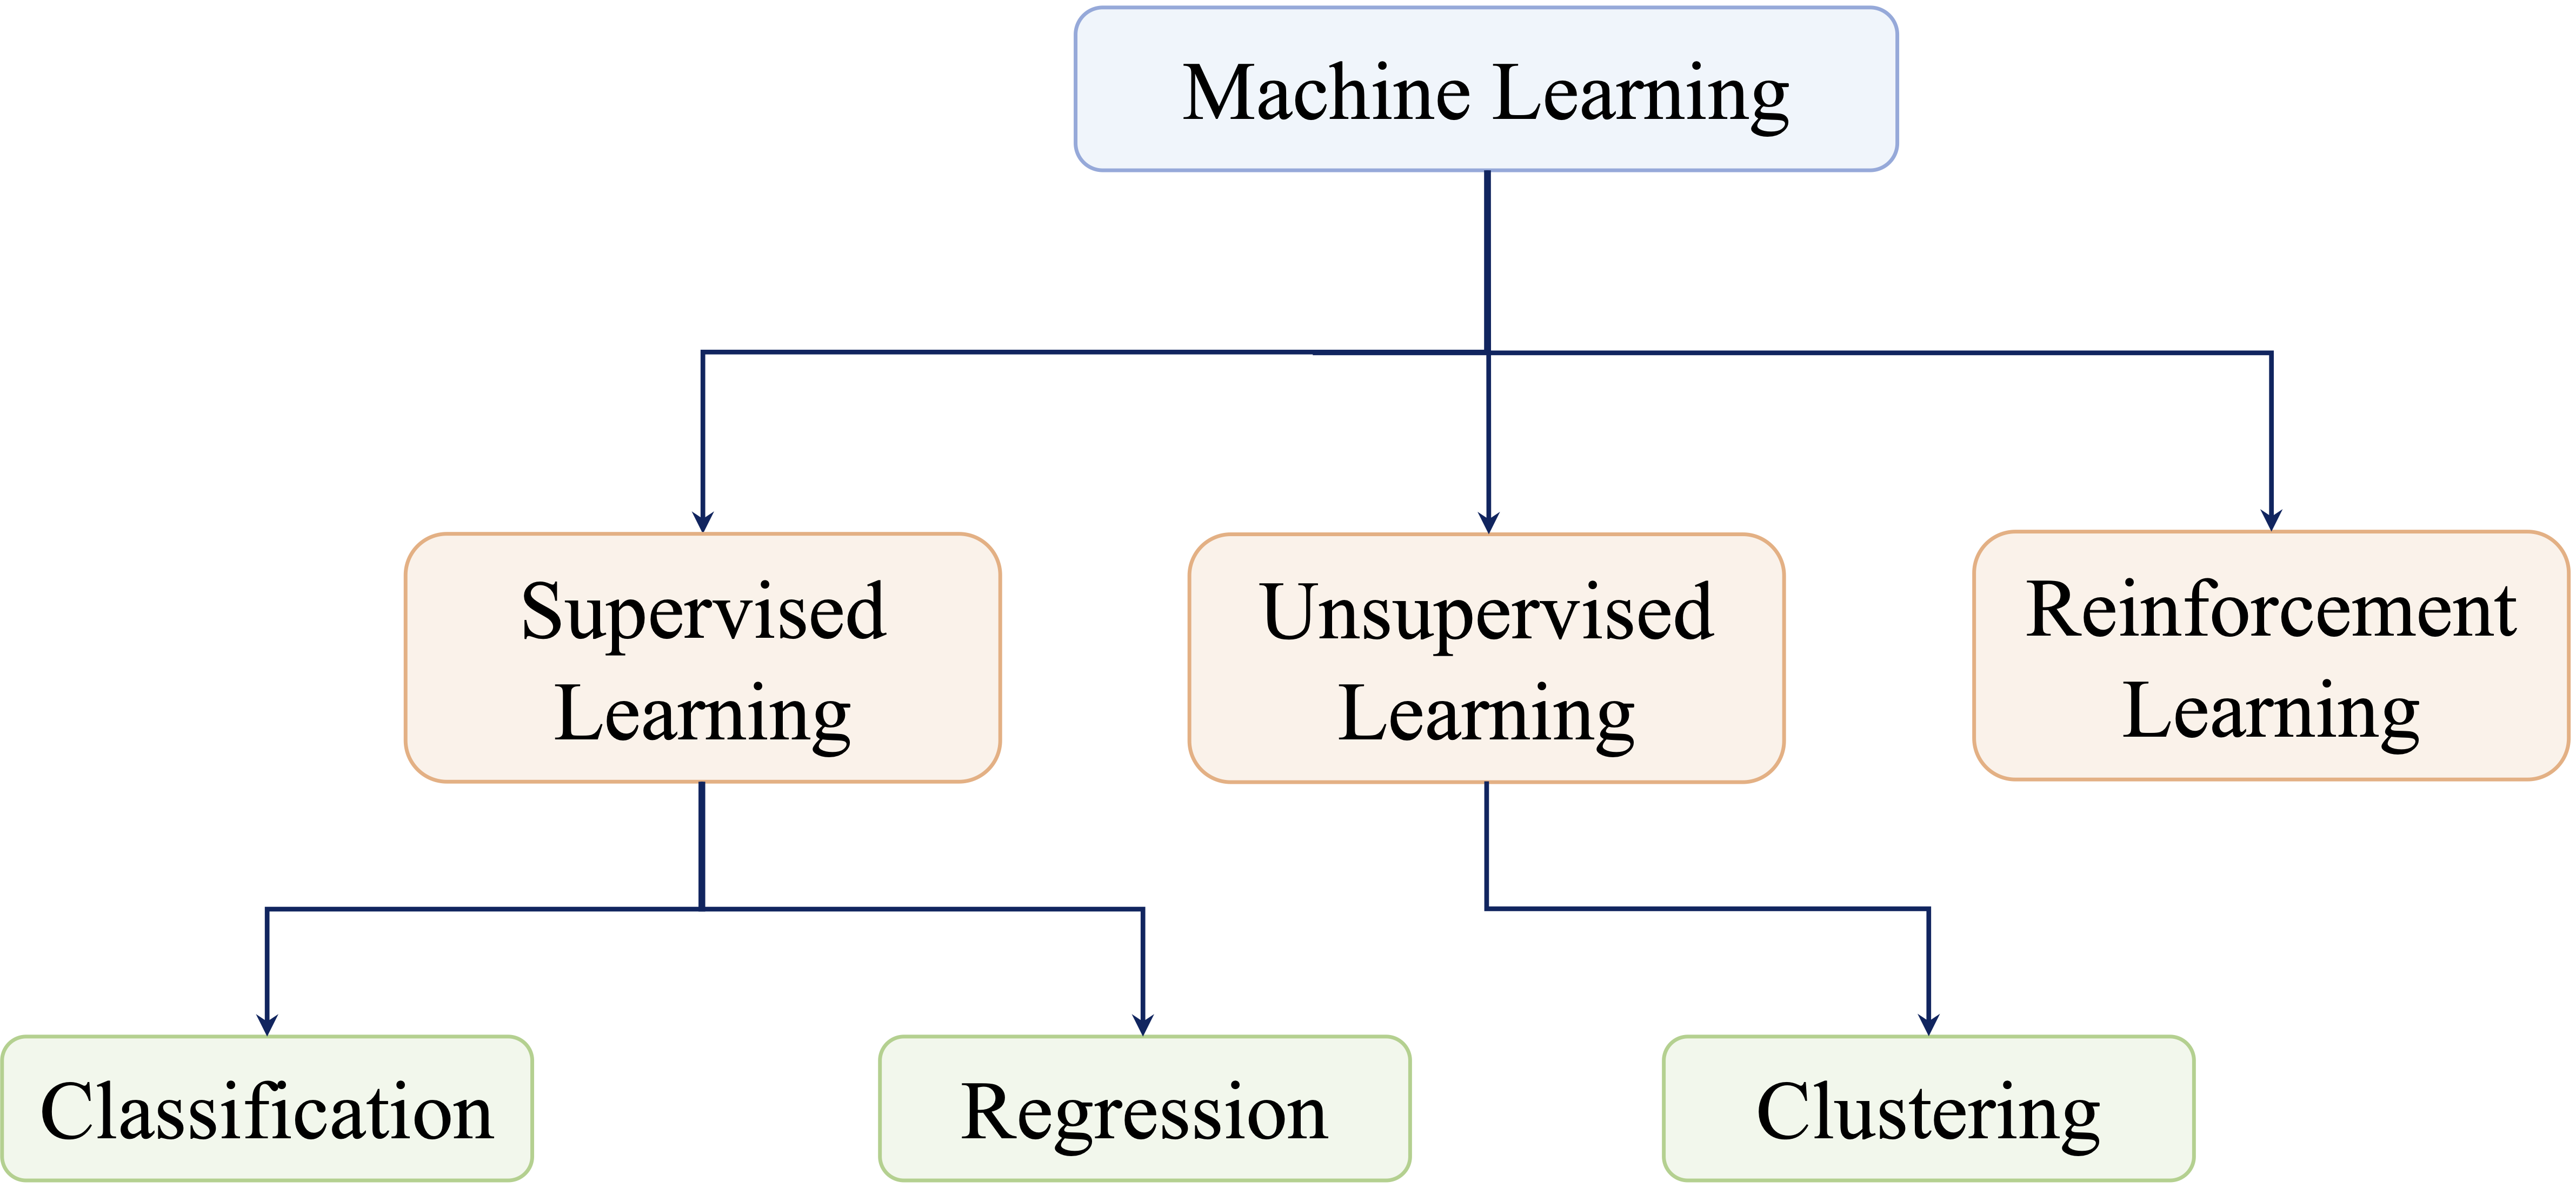
\includegraphics[width=0.8\linewidth,height=\textheight,keepaspectratio]{images/ch2_machine_learning.png}

}

\caption{\label{fig-machine-learning}Machine learning tasks can be
broadly categorized into supervised learning, unsupervised learning, and
reinforcement learning, which differ in how models learn from data and
what goals they pursue.}

\end{figure}%

Table \ref{tbl-ch2-machine-learning} summarizes how the main types of
machine learning differ in terms of input data, learning objectives, and
example applications.

\begin{table}

\caption{\label{tbl-ch2-machine-learning}Comparison of supervised,
unsupervised, and reinforcement learning tasks.}

\centering{

\centering
\begin{tabular}[t]{>{}l>{\raggedright\arraybackslash}p{7em}>{\raggedright\arraybackslash}p{12em}>{\raggedright\arraybackslash}p{12em}}
\toprule
Learning.Type & Input.Data & Goal & Example.Application\\
\midrule
\textcolor{black}{Supervised} & Labeled (X, Y) & Learn a mapping from inputs to outputs & Spam detection, disease diagnosis\\
\textcolor{black}{Unsupervised} & Unlabeled (X) & Discover hidden patterns or structure & Customer segmentation, anomaly detection\\
\textcolor{black}{Reinforcement} & Agent + Environment & Learn optimal actions through feedback & Game playing, robotic control\\
\bottomrule
\end{tabular}

}

\end{table}%

In this book, we focus primarily on supervised and unsupervised
learning, as they are most relevant for practical problems involving
structured, tabular data. In the subsections that follow, we explore
each of the three main branches of machine learning, beginning with
supervised learning, the most widely used and foundational approach.

\subsection*{Supervised Learning}\label{supervised-learning}
\addcontentsline{toc}{subsection}{Supervised Learning}

Supervised learning refers to situations where models are trained on
\emph{labeled data}---datasets that include both input variables and
known outcomes. Consider the task of detecting fraudulent credit card
transactions. Historical data contains records labeled as either
``fraud'' or ``legitimate,'' and the goal is to build a model that
learns from these examples to predict whether a future transaction is
likely to be fraudulent. This setup characterizes supervised learning.

Supervised learning is the most widely used approach in machine
learning. It involves training a model on a dataset where each
observation consists of input variables (features) and a corresponding
known outcome (label). The model learns a relationship between the
inputs, typically denoted as \(X\), and the output \(Y\), with the aim
of making accurate predictions on new, unseen data. This learning
process is summarized in Figure \ref{fig-supervised-learning}.

\begin{figure}[H]

\centering{

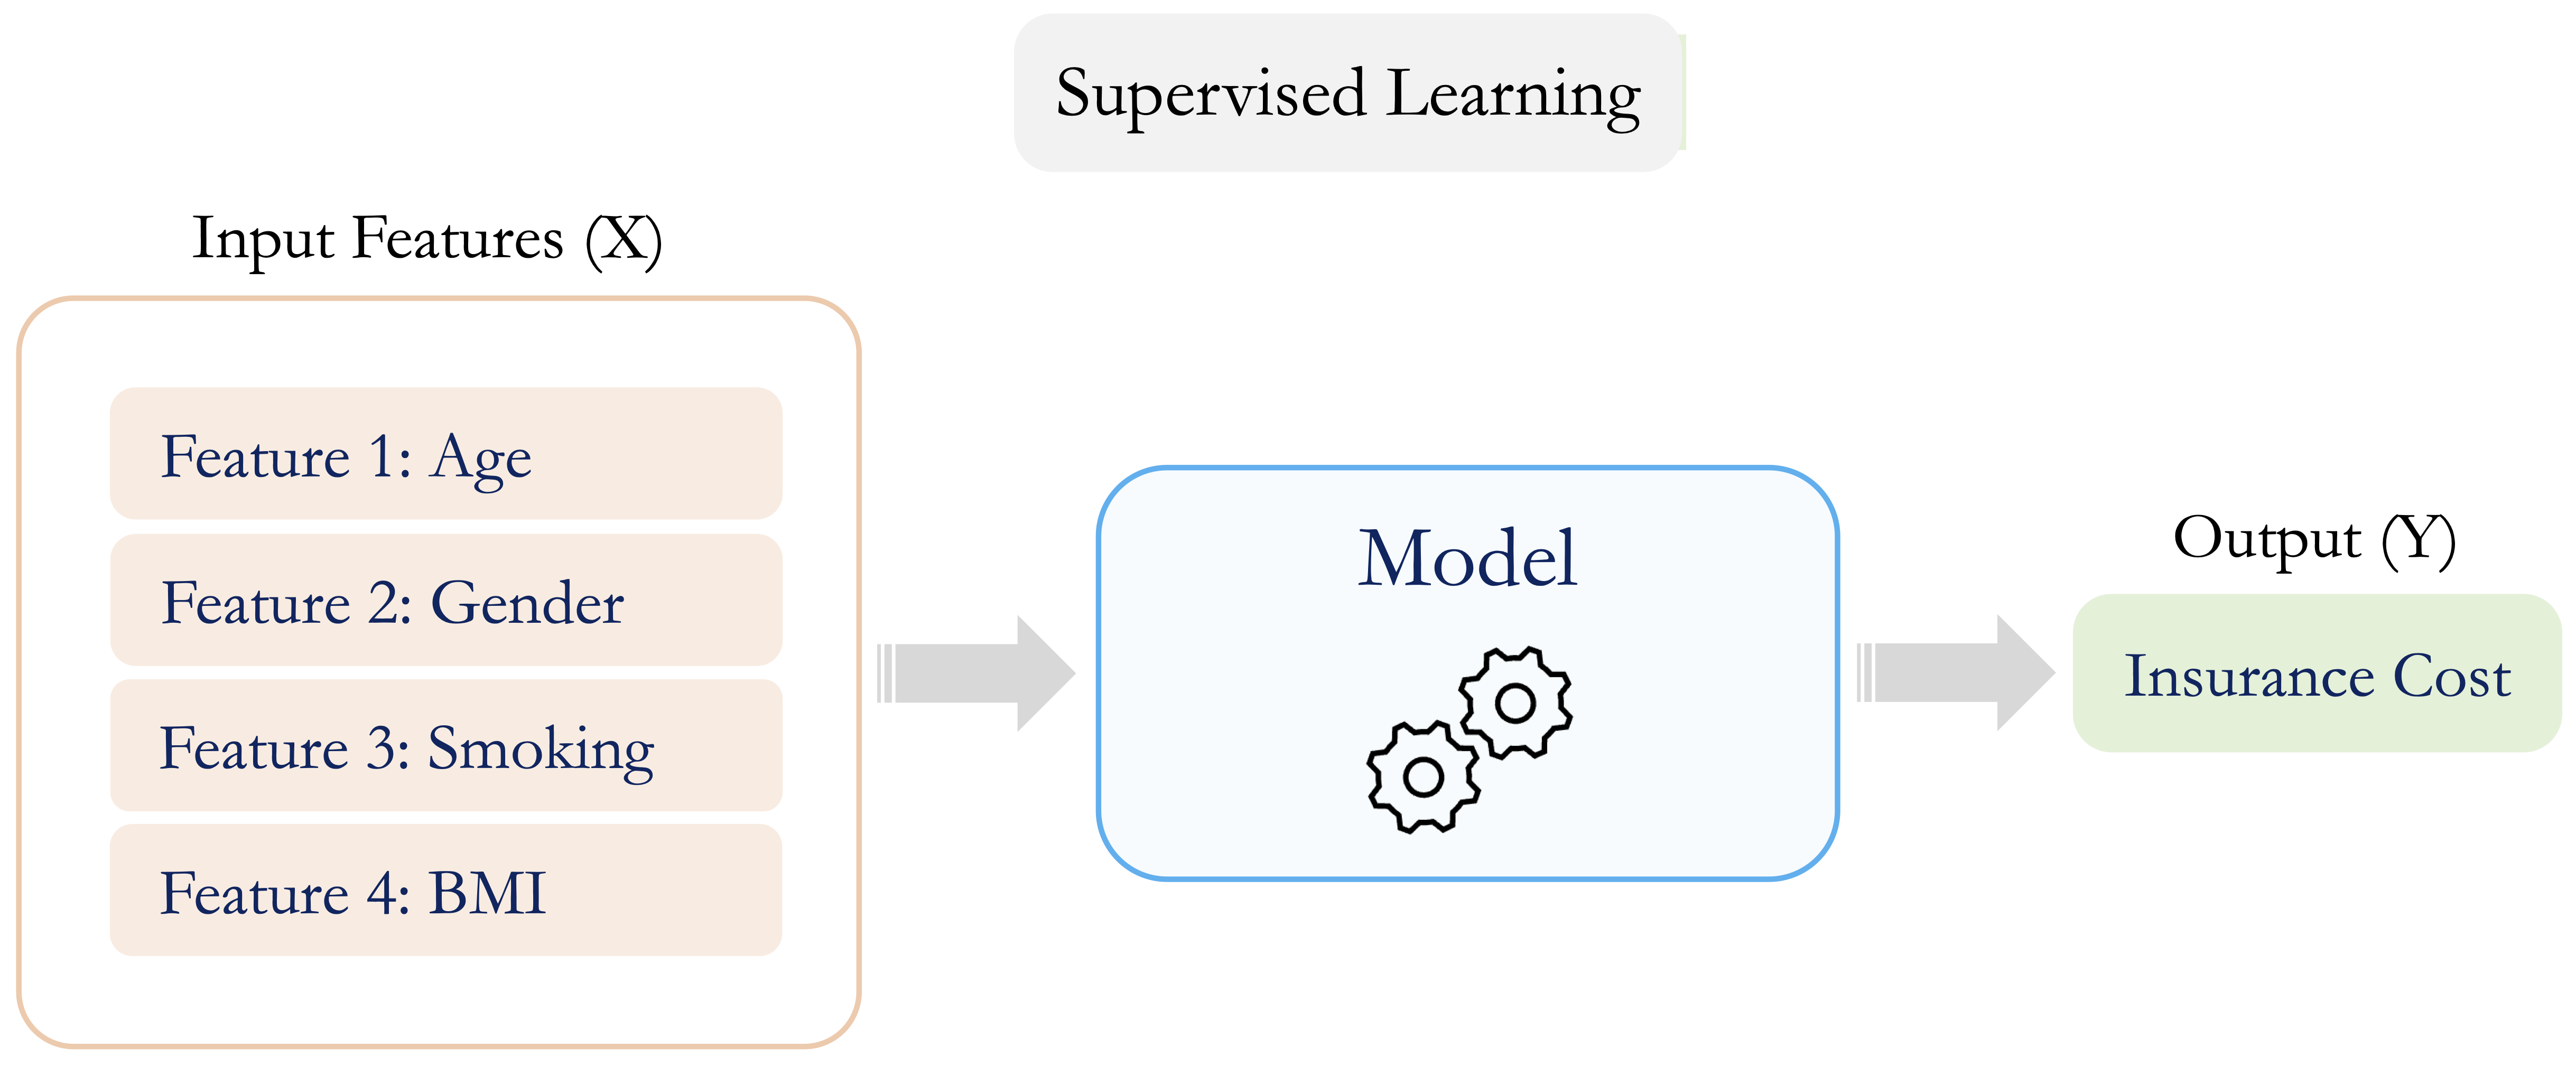
\includegraphics[width=0.85\linewidth,height=\textheight,keepaspectratio]{images/ch2_supervised_learning.png}

}

\caption{\label{fig-supervised-learning}Supervised learning methods aim
to predict the output variable (Y) based on input features (X).}

\end{figure}%

Supervised learning problems fall into two major categories. In
\emph{classification}, the model assigns data points to discrete
classes, for example, identifying spam emails or diagnosing whether a
tumor is benign or malignant. In \emph{regression}, the model predicts
continuous values, such as housing prices or future product demand.

This learning paradigm powers many systems we interact with daily, from
recommendation engines to credit scoring tools and automated medical
diagnostics. In this book, we introduce a range of supervised learning
techniques, including k-Nearest Neighbors (Chapter
\ref{sec-ch7-classification-knn}), Naïve Bayes classifiers (Chapter
\ref{sec-ch9-bayes}), decision trees and random forests (Chapter
\ref{sec-ch11-tree-models}), and regression models (Chapter
\ref{sec-ch10-regression}). Later chapters provide hands-on examples
demonstrating how to implement these models, assess their accuracy, and
interpret their results in real-world applications.

\subsection*{Unsupervised Learning}\label{unsupervised-learning}
\addcontentsline{toc}{subsection}{Unsupervised Learning}

How can we make sense of data when no outcomes are specified? This is
the central aim of unsupervised learning: analyzing datasets without
predefined labels to uncover hidden patterns, natural groupings, or
internal structure. In contrast to supervised learning, which relies on
known outputs to guide learning, unsupervised learning is primarily
\emph{exploratory}, aiming to reveal how the data is organized without a
specific target in mind.

Among unsupervised techniques, \emph{clustering} is one of the most
widely used and practically valuable. It groups similar observations
based on shared characteristics, offering insight where no labels exist.
Consider an online retailer seeking to better understand its customers.
By clustering data on purchase histories and browsing behavior, the
marketing team identifies three distinct segments: budget-conscious deal
seekers, loyal repeat customers, and infrequent high-value buyers. This
insight enables them to design targeted strategies, such as offering
discounts to price-sensitive shoppers, loyalty rewards for repeat
buyers, and personalized recommendations for premium customers, thereby
increasing engagement and optimizing campaign effectiveness.

Clustering enables data-driven decision-making by revealing structure
that may not be visible through summary statistics alone. It is
particularly useful when labels are unavailable, expensive to collect,
or when the objective is to explore the data's structure before applying
predictive models.

We return to clustering in Chapter \ref{sec-ch13-clustering}, where we
examine how it can guide segmentation, anomaly detection, and pattern
discovery using real-world examples.

\subsection*{Reinforcement Learning}\label{reinforcement-learning}
\addcontentsline{toc}{subsection}{Reinforcement Learning}

How can an agent learn to make better decisions through trial and error?
This is the central question of reinforcement learning, a branch of
machine learning where an agent interacts with an environment, receives
feedback in the form of rewards or penalties, and uses this feedback to
improve its behavior over time. Unlike supervised learning, which
depends on labeled datasets, and unsupervised learning, which seeks
patterns in unlabeled data, reinforcement learning is driven by
experience and feedback from actions.

A central goal of reinforcement learning is to learn an optimal policy:
a strategy that selects actions in each state to maximize the expected
cumulative reward. This framework is especially effective in
environments where decisions are interdependent and the consequences of
actions may only become apparent after a delay.

This learning paradigm has enabled significant advances in fields such
as robotics, where agents learn to navigate or manipulate physical
environments; game-playing systems, including AlphaGo and OpenAI Five,
which develop winning strategies through self-play; and dynamic decision
systems used in adaptive pricing, inventory management, and personalized
recommendations.

Although reinforcement learning is a powerful and rapidly evolving area
of machine learning, it falls outside the scope of this book. Our focus
is on supervised and unsupervised learning methods, which are more
commonly used in applications involving structured data. For readers
interested in reinforcement learning, the textbook
\href{http://incompleteideas.net/book/the-book-2nd.html}{\emph{Reinforcement
Learning: An Introduction}} by Sutton and Barto (Sutton, Barto, et al.
1998) provides a comprehensive introduction to the topic.

\section{Chapter Summary and
Takeaways}\label{chapter-summary-and-takeaways-1}

This chapter introduced the foundational concepts that define the field
of data science and its close connection to machine learning. We began
by defining data science as an interdisciplinary field that transforms
raw data into actionable insights, drawing from statistics, programming,
and domain expertise. Through real-world examples, we illustrated its
growing relevance across diverse domains, from healthcare to finance.

A central focus was the \emph{Data Science Workflow}, a structured yet
iterative framework that guides projects from problem understanding
through data preparation, modeling, evaluation, and deployment. This
workflow serves as the backbone for the rest of the book, helping you
relate individual techniques to the broader process of building
data-driven solutions.

We also explored \emph{machine learning} as the core engine of modern
modeling. You learned how supervised learning uses labeled data to
predict outcomes, how unsupervised learning reveals structure in
unlabeled datasets, and how reinforcement learning enables agents to
learn through feedback and interaction. A comparison of these approaches
clarified their inputs, objectives, and typical applications.

Key takeaways:

\begin{itemize}
\item
  \emph{Data science is not just about data}---it is about asking
  meaningful questions, structuring analysis, and generating insight.
\item
  \emph{The workflow matters}---progress comes not from isolated steps
  but from thoughtful iteration across stages.
\item
  \emph{Machine learning enables automation and prediction}---and is
  most effective when applied within a structured process guided by
  clear goals.
\end{itemize}

In the next chapter, we turn to \emph{data preparation}, the practical
starting point for most data science projects. You will learn how to
clean, structure, and transform raw datasets into a form ready for
analysis and modeling.

\section{Exercises}\label{sec-ch2-exercises}

The exercises below are designed to reinforce the key ideas introduced
in this chapter. They progress from basic definitions and conceptual
understanding to applied scenarios, model evaluation, ethical
considerations, and personal reflection. These questions support both
individual learning and classroom discussion, and they are intended to
help you build fluency with the data science workflow and the role of
machine learning within it.

\begin{enumerate}
\def\labelenumi{\arabic{enumi}.}
\item
  Define \emph{data science} in your own words. What makes it an
  interdisciplinary field?
\item
  How does \emph{machine learning} differ from traditional rule-based
  programming?
\item
  Why is \emph{domain knowledge} important in a data science project?
\item
  What is the difference between \emph{data} and \emph{information}? How
  does the DIKW Pyramid illustrate this transformation?
\item
  How is machine learning related to \emph{artificial intelligence}? In
  what ways do they differ?
\end{enumerate}

\subsubsection*{Exploring the Data Science
Workflow}\label{exploring-the-data-science-workflow}
\addcontentsline{toc}{subsubsection}{Exploring the Data Science
Workflow}

\begin{enumerate}
\def\labelenumi{\arabic{enumi}.}
\setcounter{enumi}{5}
\item
  Why is the \emph{Problem Understanding} phase essential to the success
  of a data science project?
\item
  The Data Science Workflow is inspired by the \emph{CRISP-DM} model.
  What does CRISP-DM stand for, and what are its key stages?
\item
  Identify two alternative methodologies to CRISP-DM that are used in
  the data science industry.
\item
  What are the primary goals of the \emph{Data Preparation} stage, and
  why is it often time-consuming?
\item
  List common data quality issues that must be addressed before modeling
  can proceed effectively.
\end{enumerate}

\subsubsection*{Applied Scenarios and Case-Based
Thinking}\label{applied-scenarios-and-case-based-thinking}
\addcontentsline{toc}{subsubsection}{Applied Scenarios and Case-Based
Thinking}

\begin{enumerate}
\def\labelenumi{\arabic{enumi}.}
\setcounter{enumi}{10}
\item
  For each of the following scenarios, identify the most relevant stage
  of the Data Science Workflow:

  \begin{enumerate}
  \def\labelenumii{\alph{enumii}.}
  \tightlist
  \item
    A financial institution is developing a system to detect fraudulent
    credit card transactions.
  \item
    A city government is analyzing traffic sensor data to optimize
    stoplight schedules.
  \item
    A university is building a model to predict which students are at
    risk of dropping out.
  \item
    A social media platform is clustering users based on their
    interaction patterns.
  \end{enumerate}
\item
  Provide an example of how exploratory data analysis (EDA) can
  influence feature engineering or model selection.
\item
  What is \emph{feature engineering}? Give two examples of engineered
  features from real-world datasets.
\item
  Why is it important to split data into training, validation, and test
  sets? What is the purpose of each?
\item
  How would you approach handling missing data in a dataset that
  includes both numerical and categorical variables?
\end{enumerate}

\subsubsection*{Applying Machine Learning
Methods}\label{applying-machine-learning-methods}
\addcontentsline{toc}{subsubsection}{Applying Machine Learning Methods}

\begin{enumerate}
\def\labelenumi{\arabic{enumi}.}
\setcounter{enumi}{15}
\item
  For each task below, classify it as \emph{supervised} or
  \emph{unsupervised} learning, and suggest an appropriate algorithm:

  \begin{enumerate}
  \def\labelenumii{\alph{enumii}.}
  \tightlist
  \item
    Predicting housing prices based on square footage and location.
  \item
    Grouping customers based on purchasing behavior.
  \item
    Classifying tumors as benign or malignant.
  \item
    Discovering topic clusters in a large collection of news articles.
  \end{enumerate}
\item
  What is \emph{overfitting}? How can it be detected and prevented?
\item
  Describe the role of \emph{cross-validation} in model evaluation.
\item
  Provide an example where classification is more appropriate than
  regression, and another where regression is preferable.
\item
  What are the trade-offs between \emph{interpretability} and
  \emph{predictive performance} in machine learning models?
\end{enumerate}

\subsubsection*{Evaluation, Bias, and
Fairness}\label{evaluation-bias-and-fairness}
\addcontentsline{toc}{subsubsection}{Evaluation, Bias, and Fairness}

\begin{enumerate}
\def\labelenumi{\arabic{enumi}.}
\setcounter{enumi}{20}
\item
  Why is \emph{accuracy} not always a reliable metric for
  classification, especially in imbalanced datasets?
\item
  Suppose only 2\% of cases in a dataset represent the positive class.
  Which metrics would be more informative than accuracy?
\item
  What is a \emph{confusion matrix}, and how is it used to calculate
  \emph{precision}, \emph{recall}, and \emph{F1-score}?
\item
  Define \emph{bias} and \emph{variance} in the context of machine
  learning. What is the \emph{bias-variance trade-off}?
\item
  Provide an example of how bias in training data can lead to biased
  model predictions in deployment.
\item
  List three practices data scientists can adopt to reduce algorithmic
  bias and promote fairness.
\end{enumerate}

\subsubsection*{Broader Reflections and
Ethics}\label{broader-reflections-and-ethics}
\addcontentsline{toc}{subsubsection}{Broader Reflections and Ethics}

\begin{enumerate}
\def\labelenumi{\arabic{enumi}.}
\setcounter{enumi}{26}
\item
  To what extent can data science workflows be automated? What are the
  potential risks of full automation?
\item
  Describe a real-world application in which machine learning
  contributed to a major positive societal impact.
\item
  Describe a real-world example where the use of machine learning led to
  controversy or harm. What could have been done differently?
\item
  How do \emph{ethics}, \emph{transparency}, and \emph{explainability}
  influence public trust in machine learning systems?
\item
  Reflect on your own learning: Which aspect of data science or machine
  learning are you most interested in exploring further, and why?
\end{enumerate}

\bookmarksetup{startatroot}

\chapter{Data Preparation in Practice: From Raw Data to
Insight}\label{sec-ch3-data-preparation}

You have just been handed a spreadsheet with hundreds of columns and
thousands of rows---missing entries, inconsistent labels, strange codes
like \texttt{-999}, and values that make no sense. How do you begin to
turn this chaos into insight?

In this chapter, we explore one of the most underestimated yet
indispensable stages in the Data Science Workflow: \emph{data
preparation}. No matter how sophisticated your algorithm, the quality of
your data will ultimately shape the trustworthiness of your results. It
is often said that data scientists spend \emph{up to 80\% of their time}
preparing data, and with good reason.

In real-world settings, data rarely arrives in a clean, analysis-ready
format. Instead, it often includes missing values, outliers,
inconsistent entries, and a mix of numerical and categorical variables.
Preparing such data means more than just ``cleaning''; it involves
thoughtful transformation, encoding, and restructuring to support both
exploration and modeling.

By contrast, datasets found on platforms like
\href{https://www.kaggle.com}{Kaggle} are typically curated and neatly
labeled, often with a clear target variable and well-posed questions.
These are excellent for learning, but they can give a misleading
impression of what real data science work entails. In practice, data is
collected for operational, not analytical, purposes, and significant
effort is required to make it useful for decision-making.

To bring data preparation techniques to life, we begin with the
\emph{diamonds} dataset from the \textbf{ggplot2} package, a structured
and relatively clean dataset that allows us to practice foundational
skills. Later in the chapter, we shift to the \emph{adult} income
dataset, where we apply the same techniques to a more realistic, messier
context.

Although this chapter focuses on data preparation, many of the steps,
such as detecting outliers, handling missing values, and transforming
variables, overlap with \emph{Exploratory Data Analysis} (Chapter
\ref{sec-ch4-EDA}) and \emph{Data Setup to Model} (Chapter
\ref{sec-ch6-setup-data}). These stages are often revisited in practice,
reflecting the iterative nature of the Data Science Workflow.

With a clear understanding of the problem and its connection to the
available data, we now move to the next step: preparing the dataset for
analysis. This step builds the foundation for meaningful insights and
reliable machine learning models, transforming raw information into
structured knowledge.

\subsection*{What This Chapter Covers}\label{what-this-chapter-covers-2}
\addcontentsline{toc}{subsection}{What This Chapter Covers}

This chapter introduces the essential techniques for transforming raw
data into a format suitable for analysis and modeling. You will learn
how to:

\begin{itemize}
\item
  Spot and manage outliers using visualization and filtering to reduce
  distortion,
\item
  Detect and impute missing values to preserve data quality and
  completeness,
\item
  Scale numerical features using min-max and z-score methods to ensure
  comparability,
\item
  Encode categorical variables through ordinal, one-hot, and frequency
  encoding for use in machine learning algorithms.
\end{itemize}

To ground these techniques, we begin by clarifying the analytical goals
of our first dataset, the \emph{diamonds} dataset, and frame the task of
price estimation as a data science problem. The chapter concludes with a
hands-on case study using the \emph{adult} income dataset, where you
will apply the full data preparation pipeline in a more complex,
real-world setting. Together, these skills form a crucial step in the
Data Science Workflow and prepare you to build models with clean,
structured, and meaningful data.

\section{\texorpdfstring{Data Preparation in Action: The \emph{diamonds}
Dataset}{Data Preparation in Action: The diamonds Dataset}}\label{sec-ch3-problem-understanding}

How can we quantify the value of a diamond? What determines why two
stones that appear nearly identical fetch vastly different prices? In
this section, we bring the concepts of data preparation to life using
the \emph{diamonds} dataset, a rich, structured collection of gem
attributes from the \textbf{ggplot2} package. It serves as our testing
ground for exploring how to clean, transform, and organize data in ways
that reveal meaningful insights.

Our central goal is to understand how features such as carat, cut,
color, and clarity contribute to price variation. But before we begin
processing the data, we must first frame the business problem and
identify the analytical questions it raises. Data preparation is not
merely technical; it is purposeful.

We focus on three guiding questions: which features have the strongest
influence on diamond price; whether consistent pricing patterns emerge
based on attributes like carat weight or cut quality; and whether the
dataset contains anomalies, such as outliers or inconsistent entries,
that must be addressed before modeling.

From a business perspective, answering these questions supports smarter
pricing and inventory strategies for jewelers and online retailers. From
a data science perspective, it ensures that our preprocessing choices,
such as filtering outliers or encoding variables, are aligned with the
real-world task at hand. This alignment between domain understanding and
technical preparation is what makes data preparation both effective and
impactful.

Later in the book, we will return to this dataset in Chapter
\ref{sec-ch10-regression}, where we use the features prepared here to
build a predictive regression model, completing the journey from raw
data to actionable insight.

\subsection*{\texorpdfstring{Overview of the \emph{diamonds}
Dataset}{Overview of the diamonds Dataset}}\label{overview-of-the-diamonds-dataset}
\addcontentsline{toc}{subsection}{Overview of the \emph{diamonds}
Dataset}

With a clear understanding of the problem and the analytical goals, we
are ready to begin working directly with the data. The first step in
data preparation is to load the dataset and explore its structure to
identify what needs to be cleaned, transformed, or encoded.

We use the \emph{diamonds} dataset from the \textbf{ggplot2} package, a
structured collection of gem characteristics such as carat weight, cut,
color, clarity, and price. This dataset serves as a clean but realistic
foundation for practicing core data preparation techniques.

The dataset includes over 50,000 rows, with each observation
representing a unique diamond. It provides 10 variables describing
physical attributes and quality ratings. To follow along in R, make sure
the \textbf{ggplot2} package is installed. If it is not yet installed,
install it with \texttt{install.packages("ggplot2")}. Then load the
package and access the dataset:

\begin{Shaded}
\begin{Highlighting}[]
\FunctionTok{library}\NormalTok{(ggplot2)    }\CommentTok{\# Load ggplot2 package}

\FunctionTok{data}\NormalTok{(diamonds)      }\CommentTok{\# Load the diamonds dataset}
\end{Highlighting}
\end{Shaded}

To get a sense of the dataset's structure, use the \texttt{str()}
function:

\begin{Shaded}
\begin{Highlighting}[]
\FunctionTok{str}\NormalTok{(diamonds)}
\NormalTok{   tibble [}\DecValTok{53}\NormalTok{,}\DecValTok{940}\NormalTok{ x }\DecValTok{10}\NormalTok{] (S3}\SpecialCharTok{:}\NormalTok{ tbl\_df}\SpecialCharTok{/}\NormalTok{tbl}\SpecialCharTok{/}\NormalTok{data.frame)}
    \SpecialCharTok{$}\NormalTok{ carat  }\SpecialCharTok{:}\NormalTok{ num [}\DecValTok{1}\SpecialCharTok{:}\DecValTok{53940}\NormalTok{] }\FloatTok{0.23} \FloatTok{0.21} \FloatTok{0.23} \FloatTok{0.29} \FloatTok{0.31} \FloatTok{0.24} \FloatTok{0.24} \FloatTok{0.26} \FloatTok{0.22} \FloatTok{0.23}\NormalTok{ ...}
    \SpecialCharTok{$}\NormalTok{ cut    }\SpecialCharTok{:}\NormalTok{ Ord.factor w}\SpecialCharTok{/} \DecValTok{5}\NormalTok{ levels }\StringTok{"Fair"}\SpecialCharTok{\textless{}}\StringTok{"Good"}\SpecialCharTok{\textless{}}\NormalTok{..}\SpecialCharTok{:} \DecValTok{5} \DecValTok{4} \DecValTok{2} \DecValTok{4} \DecValTok{2} \DecValTok{3} \DecValTok{3} \DecValTok{3} \DecValTok{1} \DecValTok{3}\NormalTok{ ...}
    \SpecialCharTok{$}\NormalTok{ color  }\SpecialCharTok{:}\NormalTok{ Ord.factor w}\SpecialCharTok{/} \DecValTok{7}\NormalTok{ levels }\StringTok{"D"}\SpecialCharTok{\textless{}}\StringTok{"E"}\SpecialCharTok{\textless{}}\StringTok{"F"}\SpecialCharTok{\textless{}}\StringTok{"G"}\SpecialCharTok{\textless{}}\NormalTok{..}\SpecialCharTok{:} \DecValTok{2} \DecValTok{2} \DecValTok{2} \DecValTok{6} \DecValTok{7} \DecValTok{7} \DecValTok{6} \DecValTok{5} \DecValTok{2} \DecValTok{5}\NormalTok{ ...}
    \SpecialCharTok{$}\NormalTok{ clarity}\SpecialCharTok{:}\NormalTok{ Ord.factor w}\SpecialCharTok{/} \DecValTok{8}\NormalTok{ levels }\StringTok{"I1"}\SpecialCharTok{\textless{}}\StringTok{"SI2"}\SpecialCharTok{\textless{}}\StringTok{"SI1"}\SpecialCharTok{\textless{}}\NormalTok{..}\SpecialCharTok{:} \DecValTok{2} \DecValTok{3} \DecValTok{5} \DecValTok{4} \DecValTok{2} \DecValTok{6} \DecValTok{7} \DecValTok{3} \DecValTok{4} \DecValTok{5}\NormalTok{ ...}
    \SpecialCharTok{$}\NormalTok{ depth  }\SpecialCharTok{:}\NormalTok{ num [}\DecValTok{1}\SpecialCharTok{:}\DecValTok{53940}\NormalTok{] }\FloatTok{61.5} \FloatTok{59.8} \FloatTok{56.9} \FloatTok{62.4} \FloatTok{63.3} \FloatTok{62.8} \FloatTok{62.3} \FloatTok{61.9} \FloatTok{65.1} \FloatTok{59.4}\NormalTok{ ...}
    \SpecialCharTok{$}\NormalTok{ table  }\SpecialCharTok{:}\NormalTok{ num [}\DecValTok{1}\SpecialCharTok{:}\DecValTok{53940}\NormalTok{] }\DecValTok{55} \DecValTok{61} \DecValTok{65} \DecValTok{58} \DecValTok{58} \DecValTok{57} \DecValTok{57} \DecValTok{55} \DecValTok{61} \DecValTok{61}\NormalTok{ ...}
    \SpecialCharTok{$}\NormalTok{ price  }\SpecialCharTok{:}\NormalTok{ int [}\DecValTok{1}\SpecialCharTok{:}\DecValTok{53940}\NormalTok{] }\DecValTok{326} \DecValTok{326} \DecValTok{327} \DecValTok{334} \DecValTok{335} \DecValTok{336} \DecValTok{336} \DecValTok{337} \DecValTok{337} \DecValTok{338}\NormalTok{ ...}
    \SpecialCharTok{$}\NormalTok{ x      }\SpecialCharTok{:}\NormalTok{ num [}\DecValTok{1}\SpecialCharTok{:}\DecValTok{53940}\NormalTok{] }\FloatTok{3.95} \FloatTok{3.89} \FloatTok{4.05} \FloatTok{4.2} \FloatTok{4.34} \FloatTok{3.94} \FloatTok{3.95} \FloatTok{4.07} \FloatTok{3.87} \DecValTok{4}\NormalTok{ ...}
    \SpecialCharTok{$}\NormalTok{ y      }\SpecialCharTok{:}\NormalTok{ num [}\DecValTok{1}\SpecialCharTok{:}\DecValTok{53940}\NormalTok{] }\FloatTok{3.98} \FloatTok{3.84} \FloatTok{4.07} \FloatTok{4.23} \FloatTok{4.35} \FloatTok{3.96} \FloatTok{3.98} \FloatTok{4.11} \FloatTok{3.78} \FloatTok{4.05}\NormalTok{ ...}
    \SpecialCharTok{$}\NormalTok{ z      }\SpecialCharTok{:}\NormalTok{ num [}\DecValTok{1}\SpecialCharTok{:}\DecValTok{53940}\NormalTok{] }\FloatTok{2.43} \FloatTok{2.31} \FloatTok{2.31} \FloatTok{2.63} \FloatTok{2.75} \FloatTok{2.48} \FloatTok{2.47} \FloatTok{2.53} \FloatTok{2.49} \FloatTok{2.39}\NormalTok{ ...}
\end{Highlighting}
\end{Shaded}

This command reveals the number of observations and variables, along
with data types and sample values. The dataset includes numerical
features such as \texttt{carat} (weight), \texttt{price}, and physical
dimensions (\texttt{x}, \texttt{y}, \texttt{z}), as well as categorical
attributes like \texttt{cut} (quality of cut), \texttt{color} (ranging
from D to J), and \texttt{clarity} (from I1 to IF). These features are
central to the modeling task we will revisit in Chapter
\ref{sec-ch10-regression}.

Here is a summary of the key variables:

\begin{itemize}
\tightlist
\item
  \texttt{carat}: weight of the diamond (ranging from 0.2 to 5.01),
\item
  \texttt{cut}: quality of the cut (Fair, Good, Very Good, Premium,
  Ideal),
\item
  \texttt{color}: color grade, from D (most colorless) to J (least
  colorless),
\item
  \texttt{clarity}: clarity grade, from I1 (least clear) to IF
  (flawless),
\item
  \texttt{depth}: total depth percentage calculated as
  \texttt{2\ *\ z\ /\ (x\ +\ y)},
\item
  \texttt{table}: width of the top facet relative to the widest point,
\item
  \texttt{x}, \texttt{y}, \texttt{z}: physical dimensions in
  millimeters,
\item
  \texttt{price}: price in US dollars (ranging from \$326 to \$18,823).
\end{itemize}

Before we can begin cleaning or transforming the data, we need to
understand the types of features we are working with. Different types of
variables require different preparation strategies. In the next section,
we examine how the features in the diamonds dataset are structured and
classified.

\section{Identifying Feature Types}\label{identifying-feature-types}

Before detecting outliers or encoding variables, it is crucial to
understand what kinds of features we are working with. Whether a
variable is numerical or categorical, and what subtype it belongs to,
will shape how we clean, transform, and model the data. Feature types
influence which visualizations make sense, which preprocessing steps are
appropriate, and how machine learning algorithms interpret input values.

Figure \ref{fig-ch3-feature-type} summarizes the main types of features
commonly encountered in data science:

\begin{figure}[H]

\centering{

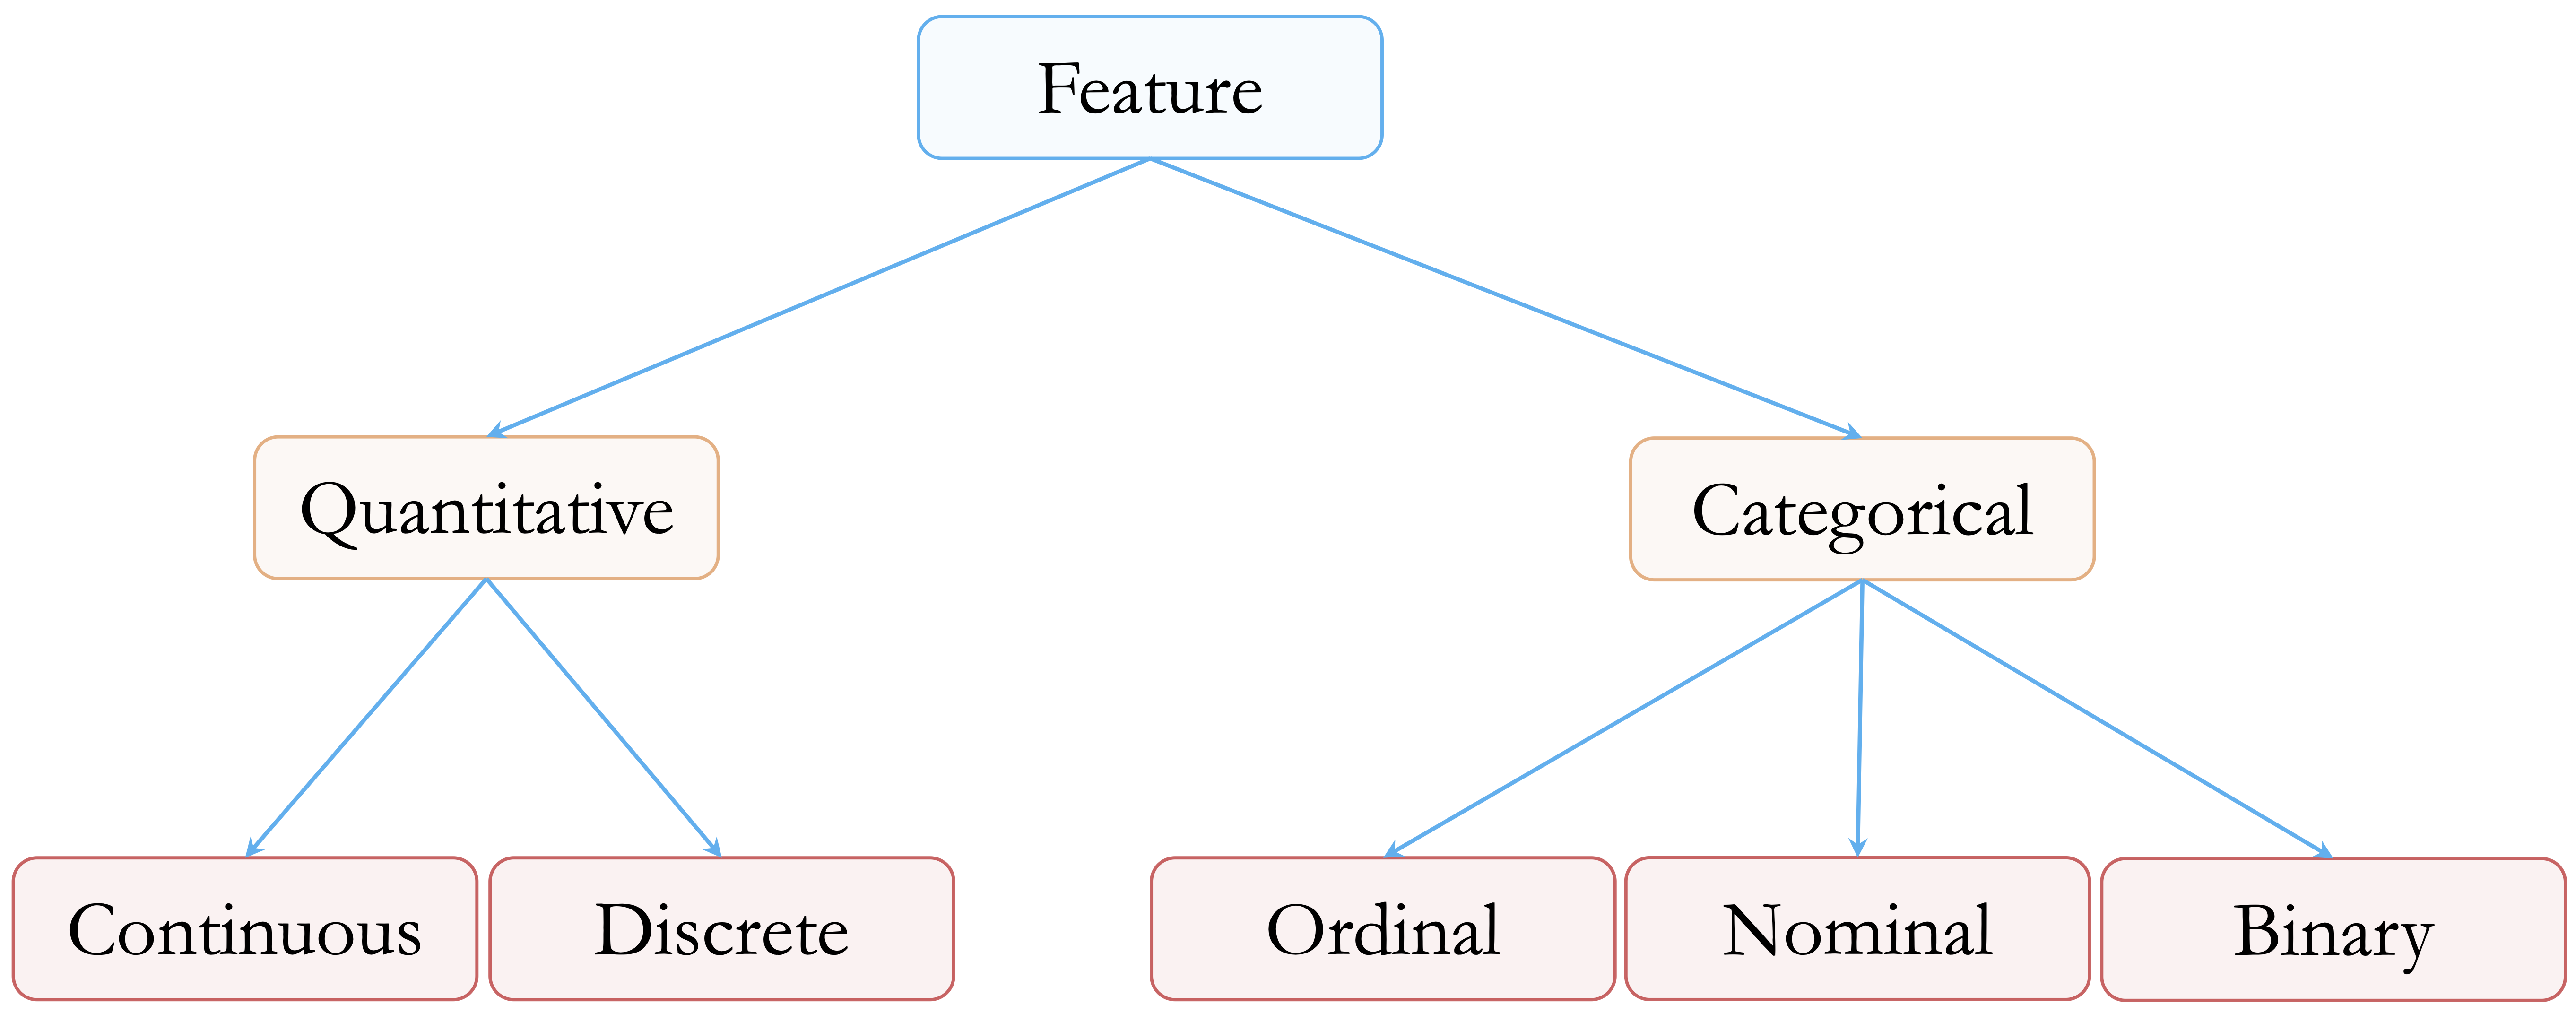
\includegraphics[width=0.85\linewidth,height=\textheight,keepaspectratio]{images/ch3_feature_type.png}

}

\caption{\label{fig-ch3-feature-type}Overview of common feature types
used in data analysis, including numerical (continuous and discrete) and
categorical (ordinal, nominal, and binary) variables.}

\end{figure}%

Features fall into two broad categories: \emph{quantitative (numerical)}
and \emph{categorical (qualitative)}, each with important subtypes.

\emph{Quantitative (Numerical) features} represent measurable
quantities:

\begin{itemize}
\item
  \emph{Continuous features} can take any value within a range. In the
  \emph{diamonds} dataset, variables such as \texttt{carat},
  \texttt{price}, \texttt{x}, \texttt{y}, \texttt{z}, and \texttt{depth}
  are continuous.
\item
  \emph{Discrete features} take on countable values, typically integers.
  Although not present in this dataset, an example might be the number
  of prior purchases or visits.
\end{itemize}

\emph{Categorical (Qualitative) features} classify observations into
groups:

\begin{itemize}
\item
  \emph{Ordinal features} have a meaningful order, though the spacing
  between levels is not necessarily equal. The \emph{diamonds} dataset
  includes ordinal variables like \texttt{cut}, \texttt{color}, and
  \texttt{clarity}. For example, \texttt{color} ranges from D to J, an
  alphabetical scale that reflects a progression from most to least
  colorless.
\item
  \emph{Nominal features} represent categories with no inherent order,
  such as product types or blood types.
\item
  \emph{Binary features} have exactly two categories, such as
  ``yes''/``no'' or ``male''/``female'', typically encoded as 0 and 1.
\end{itemize}

Although the \emph{diamonds} dataset does not contain discrete, nominal,
or binary features, these are frequently encountered in real-world
datasets and require distinct handling strategies.

Understanding feature types helps determine which preprocessing
techniques are appropriate. Numerical features often benefit from
scaling, typically using methods such as min-max scaling or z-score
scaling. Ordinal features are usually encoded with ordinal encoding to
preserve their ranking, although one-hot encoding may be used when the
rank is not relevant to the analysis. Nominal features, lacking any
inherent order, are best handled using one-hot encoding to represent
each category as a separate binary feature.

In R, how a variable is stored affects its treatment during analysis.
Continuous variables are usually stored as \texttt{numeric}, while
discrete ones are often \texttt{integer}. Categorical variables appear
as \texttt{factor} objects, which may be either ordered or unordered.
You can inspect these using \texttt{str()} for the full dataset, or use
\texttt{class()} and \texttt{typeof()} to examine specific variables.

\begin{quote}
\emph{Tip:} Always check how R interprets your variables. For example, a
feature that is conceptually ordinal may be treated as a nominal
\texttt{factor} unless explicitly declared as \texttt{ordered\ =\ TRUE}.
\end{quote}

Now that we understand the structure of our features, we are ready to
begin preparing them, starting with identifying outliers that may
distort our analysis.

\section{Key Considerations for Data
Preparation}\label{key-considerations-for-data-preparation}

Effective data preparation serves as the bridge between raw input and
meaningful statistical analysis. To prepare the \emph{diamonds} dataset
for modeling, we focus on three interrelated priorities: ensuring data
quality, engineering relevant features, and transforming variables into
suitable formats.

First, data quality is essential. We need to ensure that the dataset is
accurate, consistent, and free from major issues. This includes
identifying missing values, spotting outliers, and resolving
inconsistencies that could introduce bias or reduce model performance.

Second, thoughtful feature engineering can add substantial value. For
example, rather than using the \texttt{x}, \texttt{y}, and \texttt{z}
dimensions separately, we might create a new variable that captures the
\emph{volume} of each diamond. This derived feature could serve as a
more interpretable and effective predictor of price.

Finally, appropriate data transformation ensures that all features are
in a format suitable for modeling. Categorical variables like
\texttt{cut} or \texttt{color} need to be encoded numerically, using
methods that respect their structure and meaning. At the same time,
numerical features may require scaling to ensure they contribute fairly
in algorithms that rely on distance or gradient-based optimization.

These three pillars---data quality, feature engineering, and
transformation---form the foundation of robust data preparation and help
ensure that our modeling efforts are grounded in clean, well-structured,
and informative data.

\section{Outliers: What They Are and Why They
Matter}\label{sec-ch3-data-pre-outliers}

Outliers are observations that stand out from the general pattern of a
dataset, extreme values that differ markedly from the rest. They can
arise from data entry errors, unusual measurement conditions, or
genuinely rare but meaningful events. Regardless of their source,
outliers can have an outsized impact on data analysis: they may distort
summary statistics, skew visualizations, and mislead machine learning
models.

Recognizing and handling outliers appropriately is especially important
in real-world applications. In finance, an unusually large transaction
could indicate fraud. In healthcare, an extreme lab result might point
to a rare diagnosis, or signal a faulty instrument. In manufacturing,
sensor readings that deviate from the norm might flag equipment failure
or process instability.

However, not all outliers are errors to be discarded. Some reflect
valuable exceptions that offer new insights. Removing them
indiscriminately risks throwing away useful information; keeping them
blindly can undermine model reliability. Sound judgment, grounded in
both statistical reasoning and domain knowledge, is essential when
deciding how to handle them.

Outlier detection can begin with visual tools such as \emph{boxplots},
\emph{histograms}, and \emph{scatter plots}, which offer intuitive ways
to spot anomalies. These methods are especially useful during the
exploratory phase of analysis. More formal techniques, such as z-scores
and interquartile range (IQR) thresholds, provide quantitative criteria
for identifying unusually high or low values.

In the next section, we apply visual tools to the \emph{diamonds}
dataset to see how outliers manifest in real data and how they might
affect our understanding of key variables.

\section{Spotting Outliers with Visual
Tools}\label{spotting-outliers-with-visual-tools}

Visualization is often the most accessible and informative way to begin
detecting outliers. It helps us identify values that stray far from the
typical range, whether due to data entry mistakes, rare but valid
events, or measurement anomalies. In this section, we apply visual
methods to the \texttt{y} variable (diamond width) from the
\emph{diamonds} dataset, a feature known to contain extreme or
implausible values that warrant closer inspection.

\subsection*{Boxplots: Visualizing and Flagging
Outliers}\label{boxplots-visualizing-and-flagging-outliers}
\addcontentsline{toc}{subsection}{Boxplots: Visualizing and Flagging
Outliers}

Boxplots provide a compact visual summary of a variable's distribution.
They highlight key statistics, such as the median and interquartile
range (IQR), while flagging unusually high or low values as potential
outliers. As shown in Figure \ref{fig-simple-boxplot}, the ``whiskers''
extend to 1.5 times the IQR from the lower and upper quartiles, and data
points beyond this range are considered outliers.

\begin{figure}[H]

\centering{

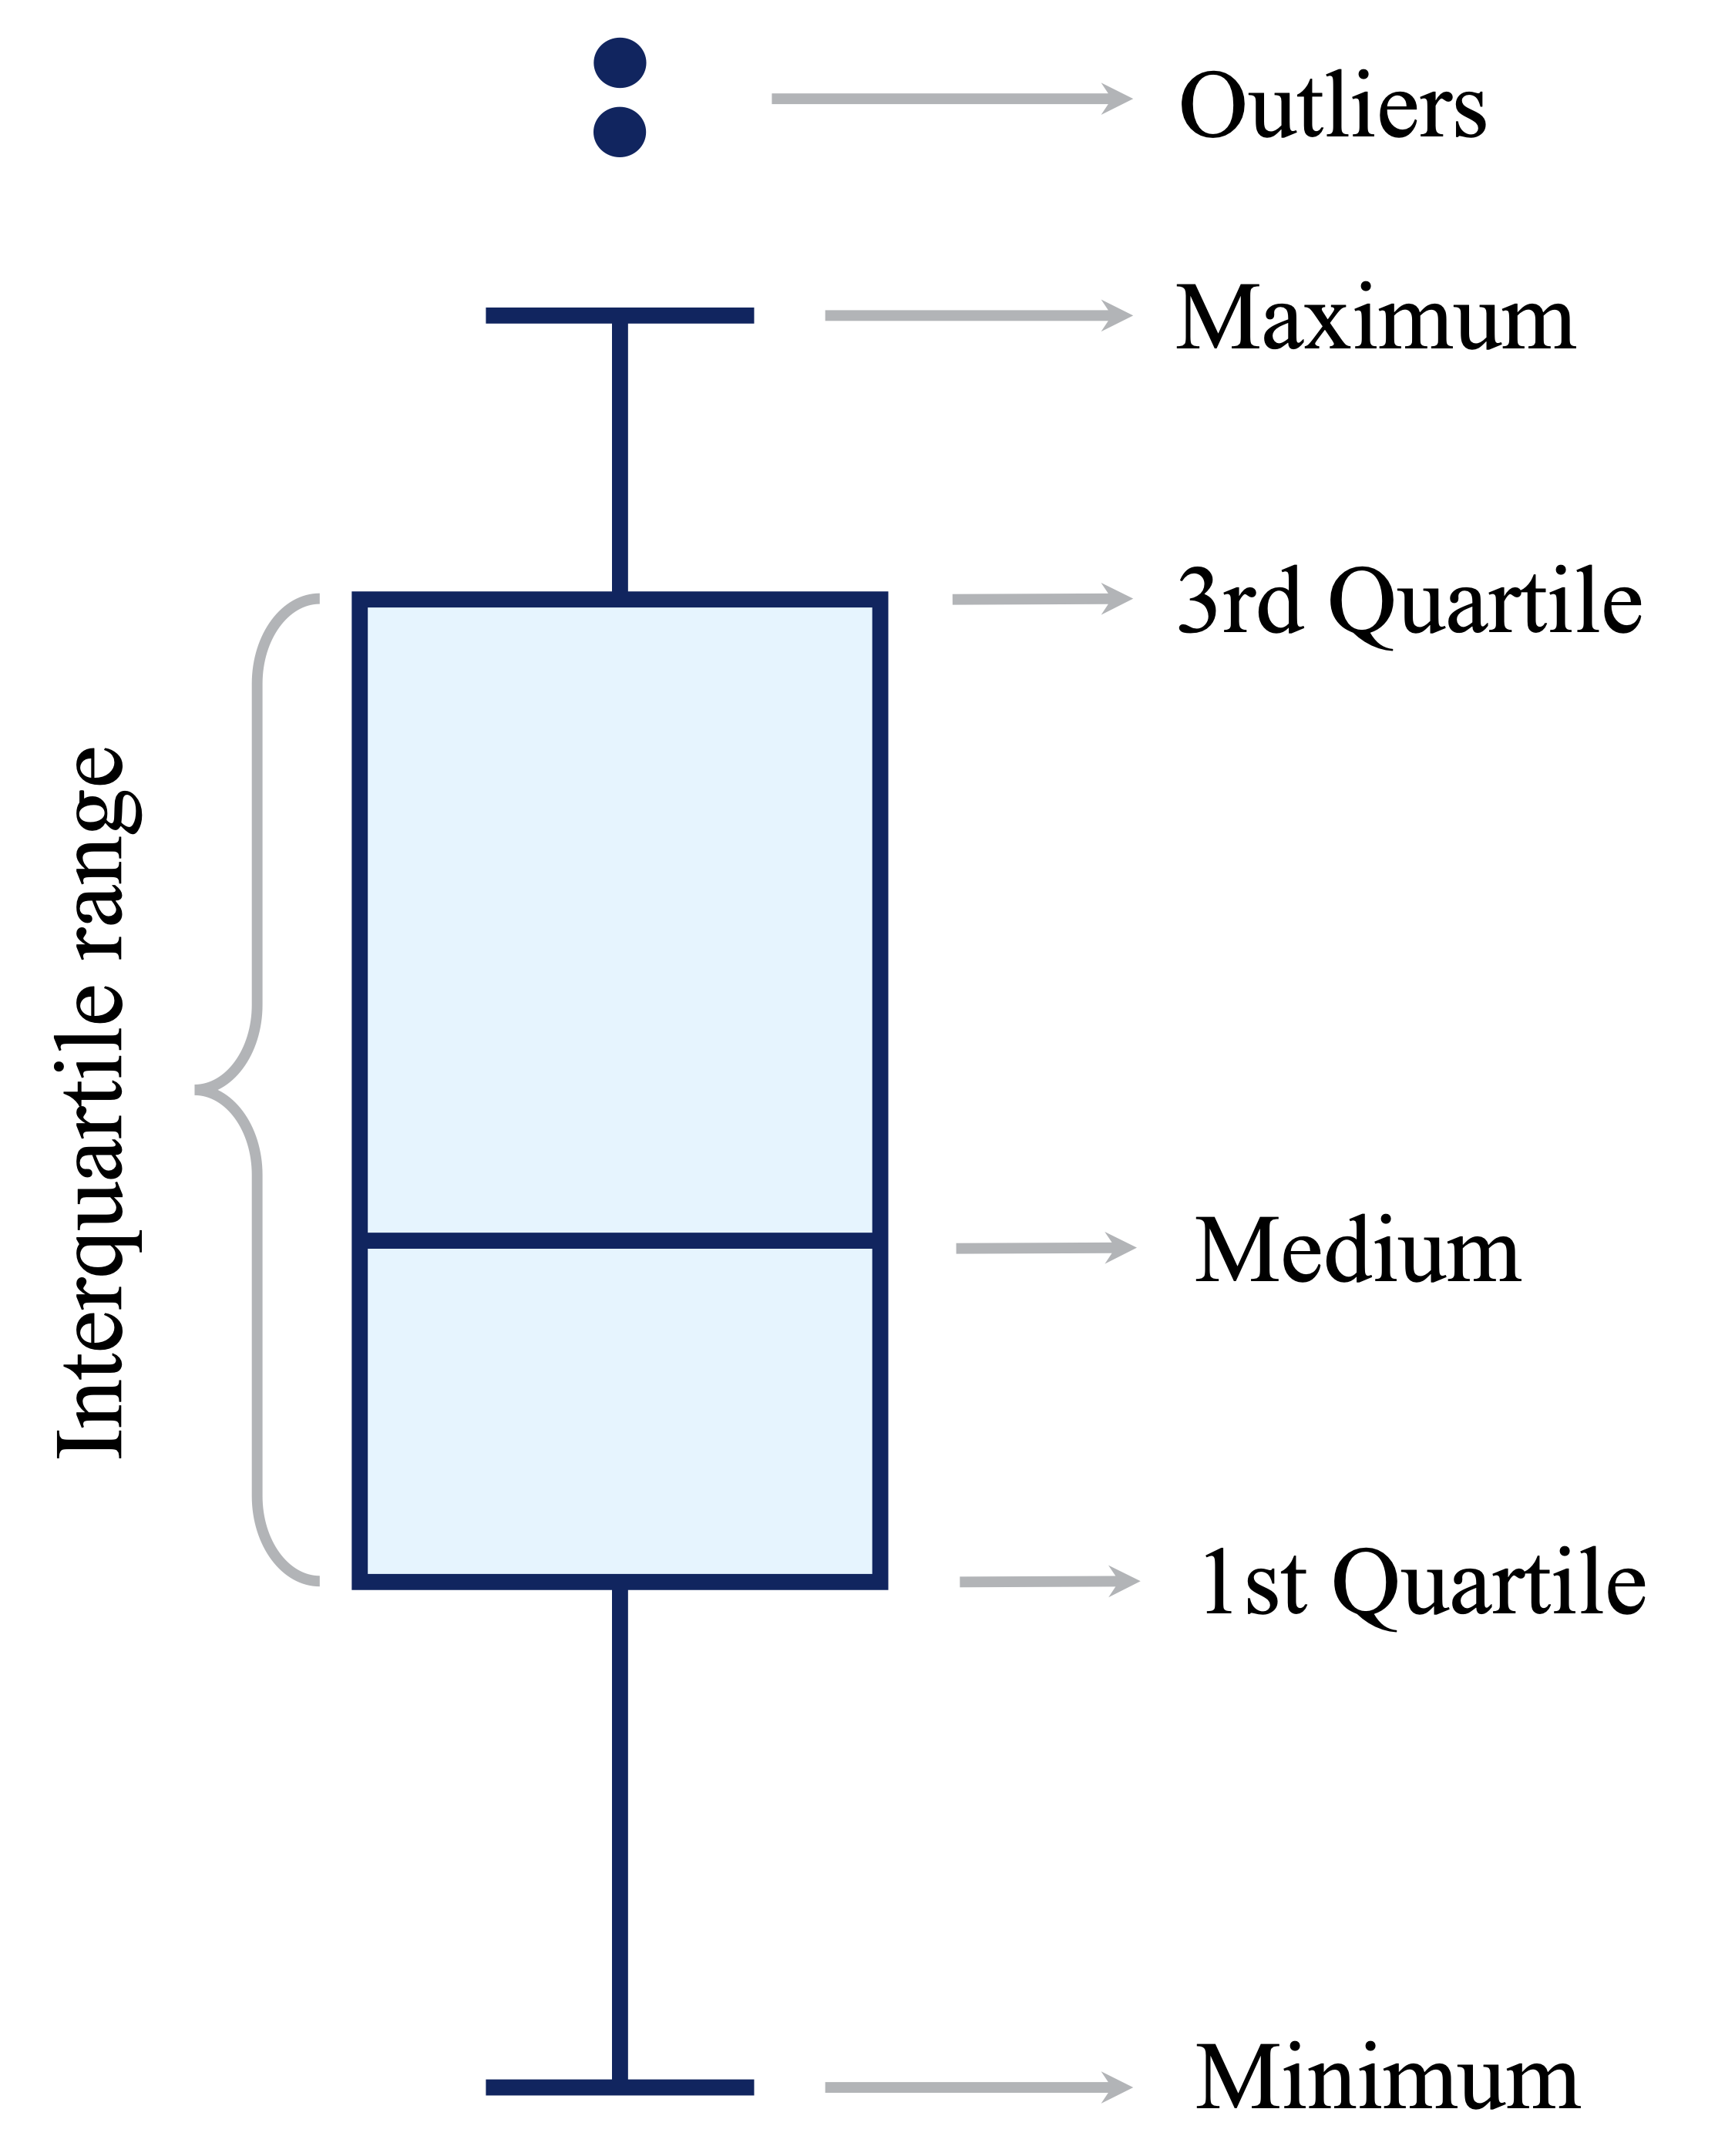
\includegraphics[width=0.4\linewidth,height=\textheight,keepaspectratio]{images/ch3_simple_boxplot.png}

}

\caption{\label{fig-simple-boxplot}Boxplots summarize a variable's
distribution and flag extreme values. Outliers are identified as points
beyond 1.5 times the interquartile range (IQR) from the quartiles.}

\end{figure}%

To see this in action, let us apply a boxplot to the \texttt{y} variable
(diamond width) in the \emph{diamonds} dataset:

\begin{Shaded}
\begin{Highlighting}[]
\FunctionTok{ggplot}\NormalTok{(}\AttributeTok{data =}\NormalTok{ diamonds) }\SpecialCharTok{+}
  \FunctionTok{geom\_boxplot}\NormalTok{(}\AttributeTok{mapping =} \FunctionTok{aes}\NormalTok{(}\AttributeTok{y =}\NormalTok{ y), }\AttributeTok{color =} \StringTok{"\#377EB8"}\NormalTok{, }\AttributeTok{fill =} \StringTok{"\#e5f4fb"}\NormalTok{)}

\FunctionTok{ggplot}\NormalTok{(}\AttributeTok{data =}\NormalTok{ diamonds) }\SpecialCharTok{+}
  \FunctionTok{geom\_boxplot}\NormalTok{(}\AttributeTok{mapping =} \FunctionTok{aes}\NormalTok{(}\AttributeTok{y =}\NormalTok{ y), }\AttributeTok{color =} \StringTok{"\#377EB8"}\NormalTok{, }\AttributeTok{fill =} \StringTok{"\#e5f4fb"}\NormalTok{) }\SpecialCharTok{+}
  \FunctionTok{coord\_cartesian}\NormalTok{(}\AttributeTok{ylim =} \FunctionTok{c}\NormalTok{(}\DecValTok{0}\NormalTok{, }\DecValTok{15}\NormalTok{))}
\end{Highlighting}
\end{Shaded}

\begin{figure}

\begin{minipage}{0.50\linewidth}
\begin{center}
\pandocbounded{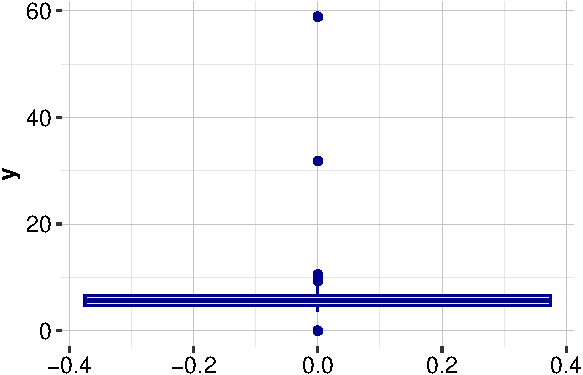
\includegraphics[keepaspectratio]{3-Data-preparation_files/figure-pdf/unnamed-chunk-4-1.pdf}}
\end{center}
\end{minipage}%
%
\begin{minipage}{0.50\linewidth}
\begin{center}
\pandocbounded{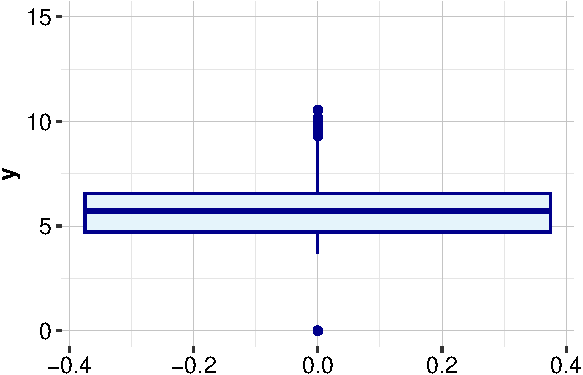
\includegraphics[keepaspectratio]{3-Data-preparation_files/figure-pdf/unnamed-chunk-4-2.pdf}}
\end{center}
\end{minipage}%

\end{figure}%

The left plot shows the full range of \texttt{y} values, where extreme
observations above 15 mm compress the rest of the distribution and
obscure the central pattern. The right plot zooms in on a more typical
range (0--15 mm), revealing that most diamond widths fall between 2 and
6 mm, with a few clear outliers.

Boxplots like these allow us to quickly identify suspicious values, such
as widths near 0 mm or above 15 mm, that are implausible for real
diamonds. These anomalies may reflect data entry errors or rare but
important cases that deserve closer inspection.

\subsection*{Histograms: Revealing Outlier
Patterns}\label{histograms-revealing-outlier-patterns}
\addcontentsline{toc}{subsection}{Histograms: Revealing Outlier
Patterns}

Histograms provide a complementary view to boxplots by showing how
values are distributed across intervals. They reveal the overall shape
of the distribution, highlight skewness, and help detect isolated spikes
or rare values that may signal outliers.

The following histogram visualizes the distribution of the \texttt{y}
variable (diamond width) using bins of width 0.5:

\begin{Shaded}
\begin{Highlighting}[]
\FunctionTok{ggplot}\NormalTok{(}\AttributeTok{data =}\NormalTok{ diamonds) }\SpecialCharTok{+}
  \FunctionTok{geom\_histogram}\NormalTok{(}\FunctionTok{aes}\NormalTok{(}\AttributeTok{x =}\NormalTok{ y), }\AttributeTok{binwidth =} \FloatTok{0.5}\NormalTok{, }\AttributeTok{color =} \StringTok{"white"}\NormalTok{, }\AttributeTok{fill =} \StringTok{"\#2C7BB6"}\NormalTok{)}
\end{Highlighting}
\end{Shaded}

\begin{center}
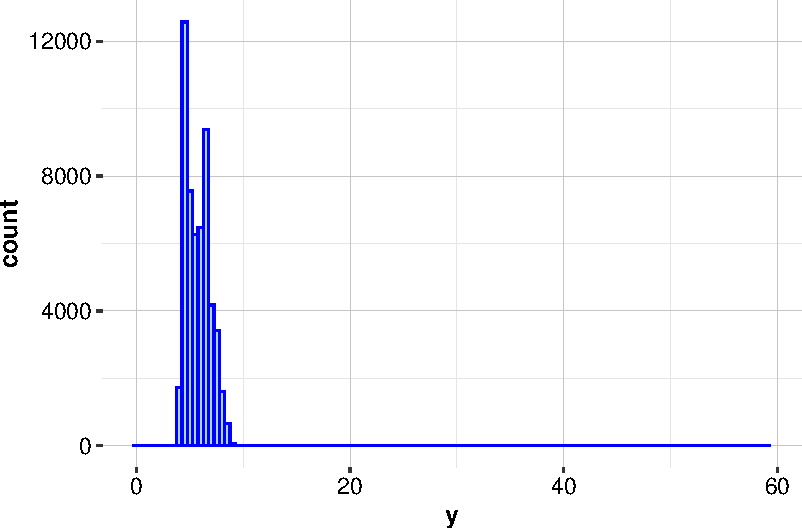
\includegraphics[width=0.6\linewidth,height=\textheight,keepaspectratio]{3-Data-preparation_files/figure-pdf/unnamed-chunk-5-1.pdf}
\end{center}

In this full-scale view, the concentration of values between 2 and 6 mm
is clear, but less frequent values, especially those beyond 15 mm, are
hard to see due to scale compression.

To focus on the rare and extreme cases, we zoom in on the lower portion
of the frequency axis:

\begin{Shaded}
\begin{Highlighting}[]
\FunctionTok{ggplot}\NormalTok{(}\AttributeTok{data =}\NormalTok{ diamonds) }\SpecialCharTok{+}
  \FunctionTok{geom\_histogram}\NormalTok{(}\AttributeTok{mapping =} \FunctionTok{aes}\NormalTok{(}\AttributeTok{x =}\NormalTok{ y), }\AttributeTok{binwidth =} \FloatTok{0.5}\NormalTok{, }\AttributeTok{color =} \StringTok{"white"}\NormalTok{, }\AttributeTok{fill =} \StringTok{"\#2C7BB6"}\NormalTok{) }\SpecialCharTok{+}
  \FunctionTok{coord\_cartesian}\NormalTok{(}\AttributeTok{ylim =} \FunctionTok{c}\NormalTok{(}\DecValTok{0}\NormalTok{, }\DecValTok{30}\NormalTok{))}
\end{Highlighting}
\end{Shaded}

\begin{center}
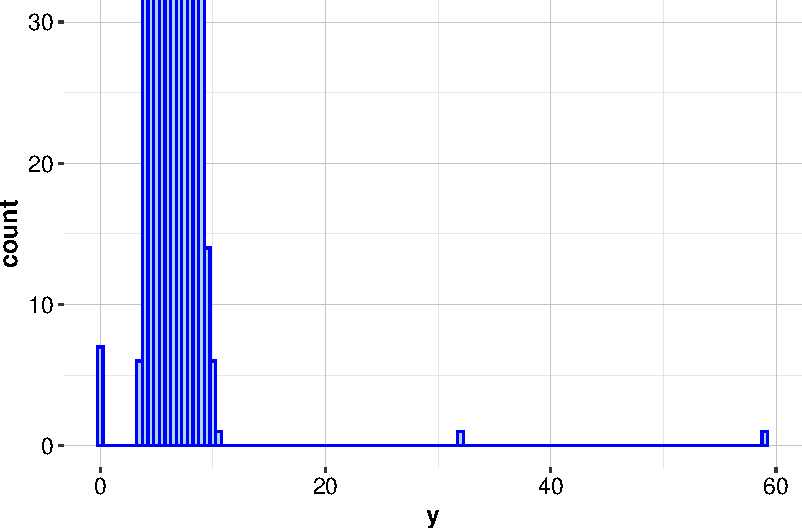
\includegraphics[width=0.6\linewidth,height=\textheight,keepaspectratio]{3-Data-preparation_files/figure-pdf/unnamed-chunk-6-1.pdf}
\end{center}

This refined view reinforces what we observed in the boxplot, namely,
the presence of unusually small or large values in the \texttt{y}
variable that fall outside the expected range. These may correspond to
data entry errors or genuine anomalies, and they warrant closer
inspection. Together with boxplots, histograms are powerful tools for
identifying and interpreting potential outliers.

\subsection*{Additional Tools for Visual Outlier
Detection}\label{additional-tools-for-visual-outlier-detection}
\addcontentsline{toc}{subsection}{Additional Tools for Visual Outlier
Detection}

In addition to boxplots and histograms, several other visualization
tools can help identify outliers in different contexts:

\begin{itemize}
\item
  \emph{Violin plots} combine the summary statistics of a boxplot with a
  mirrored density curve, offering insight into both distribution shape
  and the presence of extreme values.
\item
  \emph{Density plots} provide a smoothed view of the data distribution,
  making it easier to detect long tails, multiple modes, or subtle
  irregularities.
\item
  \emph{Scatter plots} are particularly useful for examining
  relationships between two variables and identifying outliers that
  deviate from general trends, especially in bivariate or multivariate
  contexts.
\end{itemize}

These tools are valuable in the early stages of analysis, when scanning
for irregular patterns or unusual cases. However, as the number of
dimensions increases, visual methods alone may no longer suffice. In
such cases, formal statistical techniques, covered later in the book,
offer more rigorous and scalable solutions for outlier detection.

Now that we have visually identified potential outliers, the next step
is to decide how to handle them: whether to remove, transform, or retain
these points based on their context and potential impact on analysis and
modeling.

\section{How to Handle Outliers}\label{sec-ch3-handle-outliers}

Why would a diamond have a width of 0 mm, or a price twenty times higher
than its peers? Outliers like these appear in nearly every real-world
dataset, and deciding what to do with them is a recurring challenge in
data science. When guiding students through messy datasets, I often hear
the same question: \emph{``Should I remove this outlier?''} My advice is
to pause and reflect. Not all outliers are errors, and not all errors
are obvious.

Once outliers have been identified, either visually or statistically,
the next step is to decide how to respond. There is no universal rule.
The best course of action depends on whether the outlier reflects a data
entry mistake, a rare but valid observation, or a meaningful signal.
Context is critical, and decisions should be shaped by the modeling
goals and the domain in which the data was collected.

Below are several practical strategies for handling outliers, each with
its own trade-offs:

\begin{itemize}
\item
  \emph{Retain the outlier} if it is a valid observation that may
  contain valuable information. For instance, in fraud detection,
  statistical outliers often correspond to precisely the cases of
  interest. In the \emph{adult} dataset, extreme values for
  \texttt{capital.gain} may reveal unique high-income individuals.
  Removing such observations could lead to a loss of predictive power or
  insight.
\item
  \emph{Replace the outlier with a missing value} when there is strong
  evidence that it is erroneous. For example, a negative carat weight or
  a repeated record likely stems from a data entry issue. Replacing such
  values with \texttt{NA} allows for flexible downstream handling,
  including imputation strategies introduced in the next section.
\item
  \emph{Flag and preserve the outlier} by creating an indicator variable
  (e.g., \texttt{is\_outlier}) to retain the observation without
  distorting the analysis. This is especially useful when the outlier
  might be informative but requires separate treatment.
\item
  \emph{Apply data transformations}, such as logarithmic or square root
  scaling, to reduce the influence of extreme values while preserving
  relative patterns.
\item
  \emph{Apply winsorization}, which replaces extreme outlier values with
  less extreme percentile values (e.g., capping values at the 1st and
  99th percentiles). This approach reduces the impact of outliers while
  retaining all observations, balancing robustness and data retention.
\item
  \emph{Use robust modeling techniques} that are less sensitive to
  outliers. Decision trees, random forests, and median-based estimators
  are designed to accommodate variability without being unduly
  influenced by extreme points.
\item
  \emph{Remove the outlier} only if the value is clearly invalid, cannot
  be reasonably corrected or imputed, and would otherwise compromise the
  integrity of the analysis. This should be considered a last resort,
  not the default action.
\end{itemize}

In general, a cautious and informed approach is best. Automatically
removing all outliers is tempting, especially for beginners, but it
risks discarding rare yet meaningful variation. A thoughtful strategy,
grounded in domain knowledge and analytical objectives, ensures that
data remains both clean and insightful.

\section{Outlier Treatment in Action}\label{outlier-treatment-in-action}

Now that we have seen how to spot outliers, how should we handle them in
practice? Let us walk through a hands-on example using the
\emph{diamonds} dataset. Take the \texttt{y} variable, which measures
diamond width. As we saw earlier, some entries are clearly implausible,
values equal to 0 or greater than 30 mm are unlikely for real diamonds
and likely stem from data entry errors or measurement glitches.

To fix these values, we turn to the \textbf{dplyr} package, part of the
\textbf{tidyverse}. It offers a powerful yet readable syntax for data
manipulation. One of its core functions, \texttt{mutate()}, allows us to
create or modify columns directly within a data frame. If \textbf{dplyr}
is not yet installed, you can add it with
\texttt{install.packages("dplyr")}. Then, load the package and apply the
following transformation:

\begin{Shaded}
\begin{Highlighting}[]
\FunctionTok{library}\NormalTok{(dplyr)  }\CommentTok{\# Load dplyr package}

\NormalTok{diamonds\_2 }\OtherTok{\textless{}{-}} \FunctionTok{mutate}\NormalTok{(diamonds, }\AttributeTok{y =} \FunctionTok{ifelse}\NormalTok{(y }\SpecialCharTok{==} \DecValTok{0} \SpecialCharTok{|}\NormalTok{ y }\SpecialCharTok{\textgreater{}} \DecValTok{30}\NormalTok{, }\ConstantTok{NA}\NormalTok{, y))}
\end{Highlighting}
\end{Shaded}

This command creates a new dataset, \texttt{diamonds\_2}, by replacing
suspicious \texttt{y} values with \texttt{NA}. The logic is simple: if
\texttt{y} is 0 or greater than 30, it is replaced; otherwise, it is
left unchanged. This kind of targeted replacement keeps the rest of the
data intact while removing values likely to distort analysis.

To verify the update, summarize the variable:

\begin{Shaded}
\begin{Highlighting}[]
\FunctionTok{summary}\NormalTok{(diamonds\_2}\SpecialCharTok{$}\NormalTok{y)}
\NormalTok{      Min. }\DecValTok{1}\NormalTok{st Qu.  Median    Mean }\DecValTok{3}\NormalTok{rd Qu.    Max.    NA}\StringTok{\textquotesingle{}s }
\StringTok{     3.680   4.720   5.710   5.734   6.540  10.540       9}
\end{Highlighting}
\end{Shaded}

This summary confirms how many values were flagged and how the range has
shifted. The extreme outliers no longer dominate the distribution, and
we can now proceed with a cleaner variable.

\emph{Try it yourself:} Repeat this process for the \texttt{x} and
\texttt{z} variables, which represent length and depth. Do they contain
similar implausible values? Replace any unusual values with \texttt{NA},
and use \texttt{summary()} to assess the results. Practicing this on
multiple variables helps reinforce the principle that outlier treatment
is part of an ongoing diagnostic mindset, not just a one-time fix.

In the next section, we will move on to the next step in the data
preparation pipeline: how to impute missing values in a statistically
informed way.

\section{Missing Values: What They Are and Why They
Matter}\label{sec-ch3-missing-values}

Missing values are not just blank entries---they are clues to a larger
story in your dataset. Like a puzzle with missing pieces, incomplete
data can hide important patterns, distort results, and mislead your
models. Before drawing conclusions or fitting algorithms, it is
essential to detect and handle missing data with care.

In R, missing values usually appear as \texttt{NA}, but in real-world
datasets, they often hide behind special codes like \texttt{-1},
\texttt{999}, or \texttt{99.9}. These placeholder values are easy to
miss, and if ignored, can quietly undermine your analysis. For instance,
in the \emph{cereal} dataset from the \textbf{liver} package (explored
in Section \ref{sec-ch13-case-study}), the \texttt{calories} variable
uses \texttt{-1} to indicate missing data. Similarly, in the \emph{bank}
marketing dataset (Section \ref{sec-ch12-case-study}), the \texttt{pday}
variable uses \texttt{-1} to signal that a client was not contacted.
Recognizing and recoding these special cases is a crucial first step.

As highlighted in the story of Abraham Wald (Section
\ref{sec-ch2-Problem-Understanding}), missing data is not always random.
Wald's insight came from what he \emph{could not} see, damage on planes
that never returned. In data science, the absence of information can be
just as telling as its presence. Overlooking this subtlety can lead to
flawed assumptions and inaccurate models.

Students often ask, ``How should we deal with missing values?'' My
advice is to avoid deleting data unless there is no alternative. While
dropping incomplete rows is fast, it is rarely the best choice. In fact,
if just 5\% of values are missing across 30 variables, removing all rows
with missing entries could eliminate up to 80\% of your dataset. That is
a steep price to pay. A more thoughtful approach, such as imputing
missing values, preserves valuable information while supporting the
goals of your analysis.

Broadly, there are two strategies for handling missing data:

\begin{itemize}
\item
  \emph{Imputation} involves estimating missing values using observed
  data. This method retains all records and helps maintain analytical
  completeness.
\item
  \emph{Removal} excludes rows or columns with missing entries. While
  sometimes necessary, this approach can significantly shrink your
  dataset and introduce bias, especially if the missingness is not
  random.
\end{itemize}

In the following sections, we will explore how to identify missing
values, understand their impact, and apply appropriate imputation
techniques to create a more complete and trustworthy dataset.

\section{Imputation Techniques}\label{imputation-techniques}

Once missing values have been identified, the next step is to choose an
appropriate strategy for estimating them. The best method depends on the
structure of the data, the analysis objectives, and how much complexity
is acceptable. Below are several commonly used approaches:

\begin{itemize}
\item
  \emph{Mean, median, or mode imputation} replaces missing entries with
  the average (for numerical variables), median (for skewed
  distributions), or the most frequent category (for categorical
  variables). These simple methods are best suited for low levels of
  missingness and relatively uniform data.
\item
  \emph{Random sampling} fills in missing values by drawing randomly
  from the observed values of the same variable. This technique
  preserves the variable's distribution better than mean imputation but
  introduces randomness into the analysis.
\item
  \emph{Predictive imputation} uses other variables in the dataset to
  estimate missing values through models such as linear regression,
  decision trees, or \emph{k}-nearest neighbors. This approach is more
  accurate when strong relationships exist between variables.
\item
  \emph{Multiple imputation} generates several completed datasets by
  repeating the imputation process multiple times and then combines
  results across them. This method accounts for uncertainty in the
  missing values and is especially useful for inference or reporting
  confidence intervals.
\end{itemize}

Selecting the right imputation method involves balancing simplicity and
precision. For numerical variables with few missing entries, mean or
median imputation often suffices. For categorical variables, mode
imputation provides a straightforward alternative. In cases with
substantial missingness or complex dependencies, predictive methods,
such as regression or \emph{k}-nearest neighbors, offer more reliable
results. If a variable is missing too frequently, it may be better to
exclude it or reconsider its role in the analysis.

In the coming example, we demonstrate the random sampling approach for
its simplicity and illustrative value. However, in real-world
applications, more advanced techniques are often preferred. Later in
this chapter and in Chapter \ref{sec-ch13-clustering} (Section
\ref{sec-ch13-case-study}), we revisit this topic using Random Forest
algorithm for imputation. This transition from basic to sophisticated
methods reflects the increasing demands of applied data science.

\subsection*{Random Sampling Imputation in
R}\label{random-sampling-imputation-in-r}
\addcontentsline{toc}{subsection}{Random Sampling Imputation in R}

Let us now put imputation into practice using the \texttt{y} variable
(diamond width) in the \emph{diamonds} dataset. Earlier, we flagged
implausible values, such as 0 or values above 30 mm, as missing
(\texttt{NA}). Our goal here is to replace those missing values using
\emph{random sampling}, a simple technique that draws replacements from
the observed, non-missing values of the same variable.

We use the \texttt{impute()} function from the \textbf{Hmisc} package,
which supports several basic imputation strategies. If the package is
not installed on your system, you can add it using
\texttt{install.packages("Hmisc")}. Then, load the package and apply the
imputation:

\begin{Shaded}
\begin{Highlighting}[]
\FunctionTok{library}\NormalTok{(Hmisc)  }\CommentTok{\# Load Hmisc package}

\NormalTok{diamonds\_2}\SpecialCharTok{$}\NormalTok{y }\OtherTok{\textless{}{-}} \FunctionTok{impute}\NormalTok{(diamonds\_2}\SpecialCharTok{$}\NormalTok{y, }\StringTok{"random"}\NormalTok{)  }\CommentTok{\# Randomly fill in missing values in y}
\end{Highlighting}
\end{Shaded}

This command replaces each \texttt{NA} in the \texttt{y} column with a
randomly selected value from the observed values, preserving the
variable's distribution. Because this technique introduces no systematic
bias, it works well in exploratory settings where preserving the shape
of the data is more important than prediction accuracy.

To assess the effect of imputation visually, the scatter plots below
show the relationship between diamond width (\texttt{y}) and price
before and after imputation:

\begin{Shaded}
\begin{Highlighting}[]
\FunctionTok{ggplot}\NormalTok{(diamonds, }\FunctionTok{aes}\NormalTok{(}\AttributeTok{x =}\NormalTok{ y, }\AttributeTok{y =}\NormalTok{ price)) }\SpecialCharTok{+} 
  \FunctionTok{geom\_point}\NormalTok{(}\AttributeTok{color =} \StringTok{"\#377EB8"}\NormalTok{, }\AttributeTok{size =} \FloatTok{0.5}\NormalTok{, }\AttributeTok{alpha =} \FloatTok{0.6}\NormalTok{) }\SpecialCharTok{+}
  \FunctionTok{labs}\NormalTok{(}\AttributeTok{title =} \StringTok{"With Outliers"}\NormalTok{, }\AttributeTok{x =} \StringTok{"Diamond Size (y)"}\NormalTok{, }\AttributeTok{y =} \StringTok{"Price"}\NormalTok{) }

\FunctionTok{ggplot}\NormalTok{(diamonds\_2, }\FunctionTok{aes}\NormalTok{(}\AttributeTok{x =}\NormalTok{ y, }\AttributeTok{y =}\NormalTok{ price)) }\SpecialCharTok{+} 
  \FunctionTok{geom\_point}\NormalTok{(}\AttributeTok{color =} \StringTok{"\#377EB8"}\NormalTok{, }\AttributeTok{size =} \FloatTok{0.5}\NormalTok{, }\AttributeTok{alpha =} \FloatTok{0.6}\NormalTok{) }\SpecialCharTok{+}
  \FunctionTok{labs}\NormalTok{(}\AttributeTok{title =} \StringTok{"After Imputation"}\NormalTok{, }\AttributeTok{x =} \StringTok{"Diamond Size (y)"}\NormalTok{, }\AttributeTok{y =} \StringTok{"Price"}\NormalTok{) }
\end{Highlighting}
\end{Shaded}

\begin{figure}

\begin{minipage}{0.50\linewidth}
\begin{center}
\pandocbounded{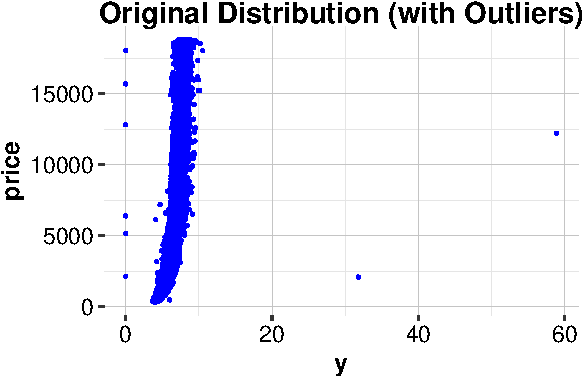
\includegraphics[keepaspectratio]{3-Data-preparation_files/figure-pdf/unnamed-chunk-10-1.pdf}}
\end{center}
\end{minipage}%
%
\begin{minipage}{0.50\linewidth}
\begin{center}
\pandocbounded{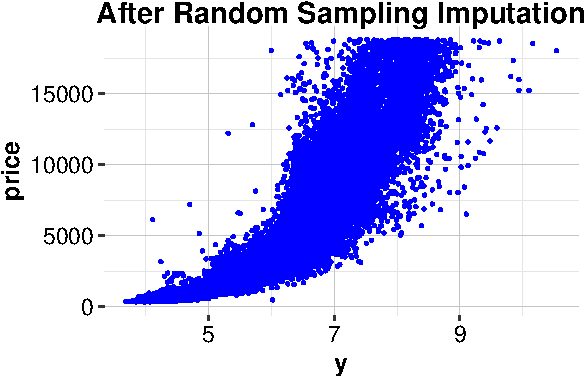
\includegraphics[keepaspectratio]{3-Data-preparation_files/figure-pdf/unnamed-chunk-10-2.pdf}}
\end{center}
\end{minipage}%

\end{figure}%

These plots illustrate that after removing implausible values and
imputing missing entries, the data retains its overall structure while
discarding extremes that could distort model training. Since price is
our eventual target variable (see Chapter \ref{sec-ch10-regression}),
this visualization also helps assess whether the cleaned \texttt{y}
values still support meaningful patterns.

\emph{Try it yourself:} Apply the same technique to the \texttt{x} and
\texttt{z} variables, which represent diamond length and depth. First
identify implausible values, recode them as \texttt{NA}, and then impute
them using random sampling. Reflect on how these changes affect the
variables' relationships with price.

\subsection*{Other Imputation
Approaches}\label{other-imputation-approaches}
\addcontentsline{toc}{subsection}{Other Imputation Approaches}

The \texttt{impute()} function also supports several simple statistical
methods, such as mean, median, and mode imputation. By default, it
performs \emph{median imputation}. For more flexible approaches, the
\texttt{aregImpute()} function from \textbf{Hmisc} can be used. It
performs predictive imputation using additive regression and
bootstrapping, which often produces more realistic estimates than
single-value replacements.

Another practical option is the \textbf{mice} (Multivariate Imputation
by Chained Equations) package. Its \texttt{mice()} function performs
\emph{multivariate} imputation, modeling each variable with missing
values as a function of the others in an iterative process. This method
is particularly useful when multiple variables contain missing values
that are correlated, as it accounts for their joint relationships and
better reflects uncertainty in the imputations. In the case study in
Chapter \ref{sec-ch13-case-study}, we use the \texttt{mice()} function
from the \textbf{mice} package to handle missing values in the
\emph{cereal} dataset, demonstrating its application in a realistic data
preparation workflow.

Although removing missing records with \texttt{na.omit()} is quick and
easy, it is usually discouraged unless a large portion of the data is
missing or the missingness is systematic. Thoughtful imputation helps
preserve valuable information and leads to more reliable results in the
next steps, such as encoding categorical variables or scaling numerical
ones.

With missing values now properly handled, the dataset is ready for
feature scaling, which ensures that numerical variables are on
comparable scales.

\section{Feature Scaling}\label{sec-ch3-feature-scaling}

What happens when one variable, such as price in dollars, spans tens of
thousands, while another, like carat weight, ranges only from 0 to 5?
Without scaling, machine learning models that rely on distances or
gradients may give disproportionate weight to features with larger
numerical ranges, regardless of their actual importance.

\emph{Feature scaling} addresses this imbalance by adjusting the range
or distribution of numerical features to make them comparable. It is
particularly important for algorithms such as \emph{k}-nearest neighbors
(Chapter \ref{sec-ch7-classification-knn}), support vector machines, and
neural networks. Scaling can also improve optimization stability in
models like logistic regression and enhance the interpretability of
coefficients.

In the \emph{diamonds} dataset, for example, \texttt{carat} ranges from
0.2 to 5, while \texttt{price} spans from 326 to 18823. Without scaling,
features like \texttt{price} may dominate the learning process, not
because they are more predictive, but simply because of their magnitude.

This section introduces two widely used scaling techniques:

\begin{itemize}
\item
  \emph{Min-Max Scaling} rescales values to a fixed range, typically
  \([0, 1]\).
\item
  \emph{Z-Score Scaling} centers values at zero with a standard
  deviation of one.
\end{itemize}

Choosing between these methods depends on the model and the structure of
the data. min-max scaling is preferred when a fixed input range is
required (as in neural networks), whereas z-score scaling is better
suited for algorithms that assume standardized input distributions or
rely on variance-sensitive optimization.

Note that scaling is not always necessary. Tree-based models, such as
decision trees and random forests, are scale-invariant and do not
require rescaled inputs. But for many other algorithms, scaling improves
model performance, convergence speed, and fairness across features.

One caution: scaling can obscure real-world units or exaggerate the
effect of outliers, especially when using min-max scaling. As always,
the choice of technique should reflect your modeling objectives and the
nature of your dataset. In the following sections, we demonstrate how to
apply each technique using the \emph{diamonds} dataset.

\section{Min-Max Scaling}\label{min-max-scaling}

When one feature ranges from 0 to 1 and another spans thousands, models
that rely on distances, like \emph{k}-nearest neighbors, may be skewed
toward features with larger scales. Min-max scaling addresses this by
rescaling each feature to a common range, typically \([0, 1]\), so that
no single variable dominates due to its units.

The transformation is defined by the formula: \[
x_{\text{scaled}} = \frac{x - x_{\text{min}}}{x_{\text{max}} - x_{\text{min}}},
\] where \(x\) is the original value, and \(x_{\text{min}}\) and
\(x_{\text{max}}\) are the minimum and maximum values of the feature.
This method ensures that the minimum value becomes 0 and the maximum
becomes 1.

Min-max scaling is especially useful for algorithms that use distance or
gradient information, including neural networks and support vector
machines. However, this technique is sensitive to outliers: extreme
values can stretch the scale, compressing most of the data into a narrow
band and reducing resolution for typical values.

\phantomsection\label{ex-min-max}
To see min-max scaling in action, we apply it to the \texttt{carat}
variable in the \emph{diamonds} dataset. This variable ranges from
approximately 0.2 to 5. We use the \texttt{minmax()} function from the
\textbf{liver} package to rescale the values to the \([0, 1]\) interval:

\begin{Shaded}
\begin{Highlighting}[]
\FunctionTok{ggplot}\NormalTok{(}\AttributeTok{data =}\NormalTok{ diamonds) }\SpecialCharTok{+}
  \FunctionTok{geom\_histogram}\NormalTok{(}\AttributeTok{mapping =} \FunctionTok{aes}\NormalTok{(}\AttributeTok{x =}\NormalTok{ carat), }\AttributeTok{bins =} \DecValTok{30}\NormalTok{,}
                 \AttributeTok{color =} \StringTok{"white"}\NormalTok{, }\AttributeTok{fill =} \StringTok{"\#2C7BB6"}\NormalTok{) }\SpecialCharTok{+}
  \FunctionTok{ggtitle}\NormalTok{(}\StringTok{"Before Min{-}Max Scaling"}\NormalTok{) }

\FunctionTok{ggplot}\NormalTok{(}\AttributeTok{data =}\NormalTok{ diamonds) }\SpecialCharTok{+}
  \FunctionTok{geom\_histogram}\NormalTok{(}\AttributeTok{mapping =} \FunctionTok{aes}\NormalTok{(}\AttributeTok{x =} \FunctionTok{minmax}\NormalTok{(carat)), }\AttributeTok{bins =} \DecValTok{30}\NormalTok{,}
                 \AttributeTok{color =} \StringTok{"white"}\NormalTok{, }\AttributeTok{fill =} \StringTok{"\#2C7BB6"}\NormalTok{) }\SpecialCharTok{+}
  \FunctionTok{ggtitle}\NormalTok{(}\StringTok{"After Min{-}Max Scaling"}\NormalTok{) }
\end{Highlighting}
\end{Shaded}

\begin{figure}

\begin{minipage}{0.50\linewidth}
\begin{center}
\pandocbounded{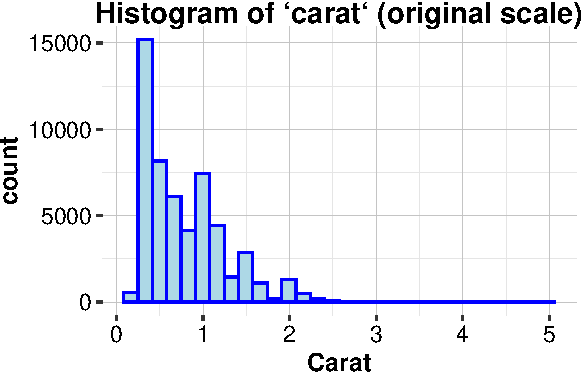
\includegraphics[keepaspectratio]{3-Data-preparation_files/figure-pdf/unnamed-chunk-11-1.pdf}}
\end{center}
\end{minipage}%
%
\begin{minipage}{0.50\linewidth}
\begin{center}
\pandocbounded{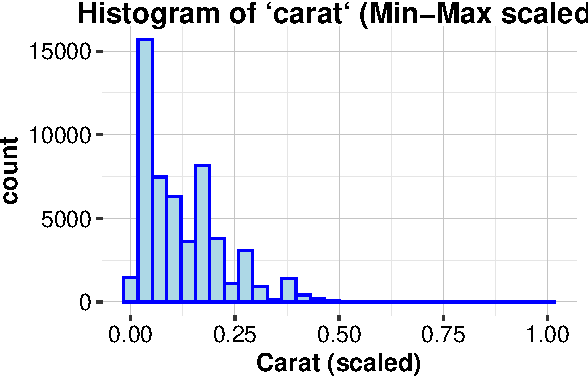
\includegraphics[keepaspectratio]{3-Data-preparation_files/figure-pdf/unnamed-chunk-11-2.pdf}}
\end{center}
\end{minipage}%

\end{figure}%

The left panel shows the raw distribution of carat values, while the
right panel displays the scaled version. After transformation, all
values fall within the \([0, 1]\) range, making this feature numerically
comparable to others. This is particularly important when modeling
techniques depend on distance or gradient magnitude.

\section{Z-Score Scaling}\label{z-score-scaling}

While min-max scaling compresses values into a fixed range, z-score
scaling, also known as standardization, centers each numerical feature
around zero and scales it to have unit variance. This technique is
especially useful for algorithms that assume normally distributed input
or rely on gradient-based optimization, such as linear regression,
logistic regression, and support vector machines.

The formula for z-score scaling is:

\[
x_{\text{scaled}} = \frac{x - \text{mean}(x)}{\text{sd}(x)},
\]

where \(x\) is the original feature value, \(\text{mean}(x)\) is the
mean of the feature, and \(\text{sd}(x)\) is its standard deviation. The
result, \(x_{\text{scaled}}\), tells us how many standard deviations the
value is from the mean.

Z-score scaling helps place features with different units or magnitudes
on a common footing. However, it is still sensitive to outliers, since
both the mean and standard deviation can be influenced by extreme
values.

\phantomsection\label{ex-zscore}
To illustrate, let us apply z-score scaling to the \texttt{carat}
variable in the \emph{diamonds} dataset. The mean and standard deviation
of \texttt{carat} are approximately 0.8 and 0.47, respectively. We use
the \texttt{zscore()} function from the \textbf{liver} package:

\begin{Shaded}
\begin{Highlighting}[]
\FunctionTok{ggplot}\NormalTok{(}\AttributeTok{data =}\NormalTok{ diamonds) }\SpecialCharTok{+}
  \FunctionTok{geom\_histogram}\NormalTok{(}\AttributeTok{mapping =} \FunctionTok{aes}\NormalTok{(}\AttributeTok{x =}\NormalTok{ carat), }\AttributeTok{bins =} \DecValTok{30}\NormalTok{,}
                 \AttributeTok{color =} \StringTok{"white"}\NormalTok{, }\AttributeTok{fill =} \StringTok{"\#2C7BB6"}\NormalTok{) }\SpecialCharTok{+}
  \FunctionTok{ggtitle}\NormalTok{(}\StringTok{"Before Z{-}Score Scaling"}\NormalTok{) }

\FunctionTok{ggplot}\NormalTok{(}\AttributeTok{data =}\NormalTok{ diamonds) }\SpecialCharTok{+}
  \FunctionTok{geom\_histogram}\NormalTok{(}\AttributeTok{mapping =} \FunctionTok{aes}\NormalTok{(}\AttributeTok{x =} \FunctionTok{zscore}\NormalTok{(carat)), }\AttributeTok{bins =} \DecValTok{30}\NormalTok{,}
                 \AttributeTok{color =} \StringTok{"white"}\NormalTok{, }\AttributeTok{fill =} \StringTok{"\#2C7BB6"}\NormalTok{) }\SpecialCharTok{+}
  \FunctionTok{ggtitle}\NormalTok{(}\StringTok{"After Z{-}Score Scaling"}\NormalTok{) }
\end{Highlighting}
\end{Shaded}

\begin{figure}

\begin{minipage}{0.50\linewidth}
\begin{center}
\pandocbounded{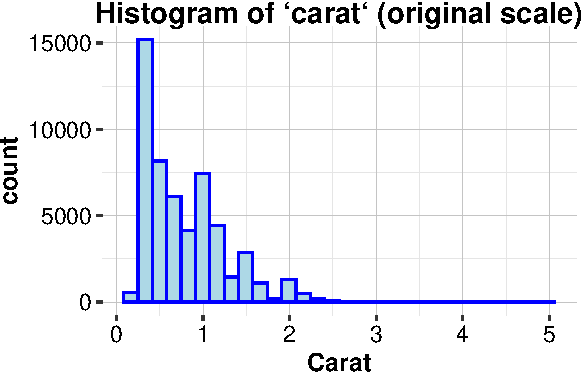
\includegraphics[keepaspectratio]{3-Data-preparation_files/figure-pdf/unnamed-chunk-12-1.pdf}}
\end{center}
\end{minipage}%
%
\begin{minipage}{0.50\linewidth}
\begin{center}
\pandocbounded{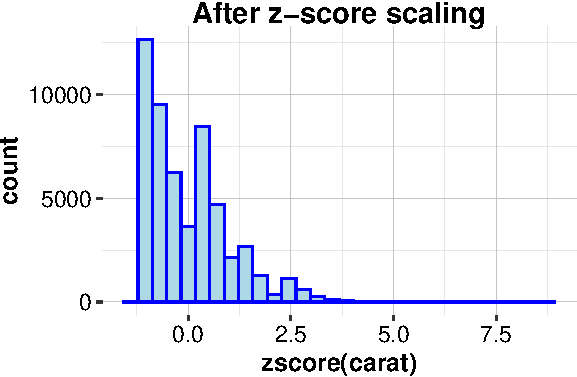
\includegraphics[keepaspectratio]{3-Data-preparation_files/figure-pdf/unnamed-chunk-12-2.pdf}}
\end{center}
\end{minipage}%

\end{figure}%

The left panel shows the original distribution of \texttt{carat} values.
The right panel displays the z-score scaled version, where the values
are centered around 0 and spread in units of standard deviation. While
the location and scale are adjusted, the shape of the distribution,
including any skewness, remains unchanged.

Note that z-score scaling does not make a variable normally distributed.
It standardizes the location and spread but preserves the shape. If the
original variable is skewed, it will remain skewed after transformation.

With numerical features now on a comparable scale, the next step is to
turn our attention to \emph{categorical variables}. Unlike numerical
features, these cannot be used directly in most models---they must be
encoded numerically. In the next section, we explore encoding strategies
for different types of categorical data, including ordinal and nominal
variables.

\section{Encoding Categorical Features}\label{sec-ch3-encoding}

Categorical features often need to be transformed into numeric format
before they can be used in machine learning models. Algorithms such as
\emph{k}-Nearest Neighbors and neural networks require numerical inputs,
and failure to encode categorical data properly can lead to misleading
results or even errors during model training.

Encoding categorical variables is a critical step in data preparation.
It allows us to incorporate qualitative information, such as quality
ratings, group memberships, or types, into models that operate on
numerical representations. In this section, we explore several encoding
techniques and illustrate their use with examples from the
\emph{diamonds} dataset, which includes the categorical variables
\texttt{cut}, \texttt{color}, and \texttt{clarity}.

The appropriate encoding strategy depends on the nature of the
categorical variable. For ordinal variables, those with an inherent
ranking, ordinal encoding preserves the order of categories using
numerical values. For example, the \texttt{cut} variable in the
\emph{diamonds} dataset ranges from ``Fair'' to ``Ideal'' and benefits
from ordinal encoding.

In contrast, nominal variables, categories without intrinsic order, are
better served by one-hot encoding. This approach creates binary
indicators for each category and is particularly effective for features
such as marital status in the \emph{bank} dataset introduced in Chapter
\ref{sec-ch12-case-study}.

In the sections that follow, we demonstrate these encoding techniques in
practice, starting with ordinal encoding and one-hot, using the
\emph{diamonds} and \emph{bank} datasets as guiding examples.

\section{Ordinal Encoding}\label{sec-ch3-ordinal-encoding}

When a categorical feature follows a meaningful order or ranking,
ordinal encoding offers a straightforward way to represent that
information numerically. Rather than treating each category as
independent, this approach assigns numerical values that reflect the
inherent order, enabling models to capture rank-based relationships.

Consider the \texttt{cut} feature in the \emph{diamonds} dataset, which
represents increasing levels of quality:

\begin{itemize}
\tightlist
\item
  ``Fair'' \(\mapsto\) 1
\item
  ``Good'' \(\mapsto\) 2
\item
  ``Very Good'' \(\mapsto\) 3
\item
  ``Premium'' \(\mapsto\) 4
\item
  ``Ideal'' \(\mapsto\) 5
\end{itemize}

In this dataset, \texttt{cut} is already stored as a \emph{factor}
variable. We can use the \texttt{factor()} function to explicitly define
its levels and assign corresponding numeric labels:

\begin{Shaded}
\begin{Highlighting}[]
\CommentTok{\# Convert an ordinal feature to numeric scores}
\NormalTok{diamonds}\SpecialCharTok{$}\NormalTok{cut\_level }\OtherTok{\textless{}{-}} \FunctionTok{factor}\NormalTok{(}
\NormalTok{  diamonds}\SpecialCharTok{$}\NormalTok{cut,}
  \AttributeTok{levels =} \FunctionTok{c}\NormalTok{(}\StringTok{"Fair"}\NormalTok{, }\StringTok{"Good"}\NormalTok{, }\StringTok{"Very Good"}\NormalTok{, }\StringTok{"Premium"}\NormalTok{, }\StringTok{"Ideal"}\NormalTok{),}
  \AttributeTok{labels =} \FunctionTok{c}\NormalTok{(}\DecValTok{1}\NormalTok{, }\DecValTok{2}\NormalTok{, }\DecValTok{3}\NormalTok{, }\DecValTok{4}\NormalTok{, }\DecValTok{5}\NormalTok{)}
\NormalTok{)}
\end{Highlighting}
\end{Shaded}

If the feature were stored as a \emph{character} variable instead, we
would first convert it to a factor before applying this transformation:

\begin{Shaded}
\begin{Highlighting}[]
\NormalTok{diamonds}\SpecialCharTok{$}\NormalTok{cut }\OtherTok{\textless{}{-}} \FunctionTok{factor}\NormalTok{(diamonds}\SpecialCharTok{$}\NormalTok{cut, }\AttributeTok{levels =} \FunctionTok{c}\NormalTok{(}\StringTok{"Fair"}\NormalTok{, }\StringTok{"Good"}\NormalTok{, }\StringTok{"Very Good"}\NormalTok{, }\StringTok{"Premium"}\NormalTok{, }\StringTok{"Ideal"}\NormalTok{))}

\NormalTok{diamonds}\SpecialCharTok{$}\NormalTok{cut\_level }\OtherTok{\textless{}{-}} \FunctionTok{as.numeric}\NormalTok{(diamonds}\SpecialCharTok{$}\NormalTok{cut)}
\end{Highlighting}
\end{Shaded}

Both approaches ensure that the encoded values preserve the correct
order of categories.

This transformation retains the ordinal structure and allows models that
recognize ordered relationships---such as linear regression, decision
trees, or ordinal logistic regression---to make more informed
predictions.

However, ordinal encoding should only be used when the order of
categories is genuinely meaningful. Applying it to nominal variables
such as ``red,'' ``green,'' and ``blue'' would wrongly imply a numerical
hierarchy, which can distort model interpretation and performance.

In summary, ordinal encoding is well suited for variables with a natural
ranking, where numerical values meaningfully represent category order.
For variables without inherent order, a different approach is needed.
The next section introduces one-hot encoding, a method designed
specifically for nominal features.

\section{One-Hot Encoding}\label{sec-ch3-one-hot-encoding}

How can we represent unordered categories, like marital status or race,
so that machine learning algorithms can work with them? \emph{One-hot
encoding} is a widely used solution. It transforms each unique category
into a separate binary column, allowing algorithms to process
categorical data without introducing artificial order.

This method is especially useful for \emph{nominal variables},
categorical features with no inherent ranking. For example, a variable
like \texttt{marital.status} in the \emph{adult} dataset includes
categories such as \texttt{Divorced}, \texttt{Married}, and
\texttt{Never-married}. One-hot encoding creates binary variables like:

\begin{itemize}
\tightlist
\item
  \texttt{marital.status\_Divorced};
\item
  \texttt{marital.status\_Married};
\item
  \texttt{marital.status\_Never-married};
\item
  \texttt{marital.status\_Separated}.
\end{itemize}

Each column indicates the presence (1) or absence (0) of a specific
category. If there are \(k\) levels, only \(k - 1\) binary columns are
needed to avoid multicollinearity---the omitted category is implicitly
captured when all others are zero.

Let us take a quick look at the \texttt{marital.status} variable in the
\emph{adult} dataset:

\begin{Shaded}
\begin{Highlighting}[]
\FunctionTok{data}\NormalTok{(adult)}

\FunctionTok{table}\NormalTok{(adult}\SpecialCharTok{$}\NormalTok{marital.status)}
   
\NormalTok{        Divorced       Married Never}\SpecialCharTok{{-}}\NormalTok{married     Separated       Widowed }
            \DecValTok{6613}         \DecValTok{22847}         \DecValTok{16096}          \DecValTok{1526}          \DecValTok{1516}
\end{Highlighting}
\end{Shaded}

The output shows the distribution of values across the five categories.
We will use one-hot encoding to transform these into model-ready binary
features. This approach ensures that all categories are represented
without assuming any order or relationship among them.

Note that one-hot encoding is essential for models that rely on distance
metrics (e.g., k-nearest neighbors, neural networks) or linear models
where numeric input is required.

\subsection{One-Hot Encoding in R}\label{one-hot-encoding-in-r}

To apply one-hot encoding in practice, we use the \texttt{one.hot()}
function from the \textbf{liver} package. This function automatically
detects categorical variables and generates a new column for each unique
level, converting them into binary indicators.

Let us apply it to the \texttt{marital.status} variable in the
\emph{adult} dataset:

\begin{Shaded}
\begin{Highlighting}[]
\CommentTok{\# One{-}hot encode the \textquotesingle{}marital.status\textquotesingle{} variable}
\NormalTok{adult\_encoded }\OtherTok{\textless{}{-}} \FunctionTok{one.hot}\NormalTok{(adult, }\AttributeTok{cols =} \FunctionTok{c}\NormalTok{(}\StringTok{"marital.status"}\NormalTok{), }\AttributeTok{dropCols =} \ConstantTok{FALSE}\NormalTok{)}

\CommentTok{\# Examine the structure of the resulting dataset}
\FunctionTok{str}\NormalTok{(adult\_encoded)}
   \StringTok{\textquotesingle{}data.frame\textquotesingle{}}\SpecialCharTok{:}    \DecValTok{48598}\NormalTok{ obs. of  }\DecValTok{20}\NormalTok{ variables}\SpecialCharTok{:}
    \ErrorTok{$}\NormalTok{ age                         }\SpecialCharTok{:}\NormalTok{ int  }\DecValTok{25} \DecValTok{38} \DecValTok{28} \DecValTok{44} \DecValTok{18} \DecValTok{34} \DecValTok{29} \DecValTok{63} \DecValTok{24} \DecValTok{55}\NormalTok{ ...}
    \SpecialCharTok{$}\NormalTok{ workclass                   }\SpecialCharTok{:}\NormalTok{ Factor w}\SpecialCharTok{/} \DecValTok{6}\NormalTok{ levels }\StringTok{"?"}\NormalTok{,}\StringTok{"Gov"}\NormalTok{,}\StringTok{"Never{-}worked"}\NormalTok{,..}\SpecialCharTok{:} \DecValTok{4} \DecValTok{4} \DecValTok{2} \DecValTok{4} \DecValTok{1} \DecValTok{4} \DecValTok{1} \DecValTok{5} \DecValTok{4} \DecValTok{4}\NormalTok{ ...}
    \SpecialCharTok{$}\NormalTok{ demogweight                 }\SpecialCharTok{:}\NormalTok{ int  }\DecValTok{226802} \DecValTok{89814} \DecValTok{336951} \DecValTok{160323} \DecValTok{103497} \DecValTok{198693} \DecValTok{227026} \DecValTok{104626} \DecValTok{369667} \DecValTok{104996}\NormalTok{ ...}
    \SpecialCharTok{$}\NormalTok{ education                   }\SpecialCharTok{:}\NormalTok{ Factor w}\SpecialCharTok{/} \DecValTok{16}\NormalTok{ levels }\StringTok{"10th"}\NormalTok{,}\StringTok{"11th"}\NormalTok{,..}\SpecialCharTok{:} \DecValTok{2} \DecValTok{12} \DecValTok{8} \DecValTok{16} \DecValTok{16} \DecValTok{1} \DecValTok{12} \DecValTok{15} \DecValTok{16} \DecValTok{6}\NormalTok{ ...}
    \SpecialCharTok{$}\NormalTok{ education.num               }\SpecialCharTok{:}\NormalTok{ int  }\DecValTok{7} \DecValTok{9} \DecValTok{12} \DecValTok{10} \DecValTok{10} \DecValTok{6} \DecValTok{9} \DecValTok{15} \DecValTok{10} \DecValTok{4}\NormalTok{ ...}
    \SpecialCharTok{$}\NormalTok{ marital.status              }\SpecialCharTok{:}\NormalTok{ Factor w}\SpecialCharTok{/} \DecValTok{5}\NormalTok{ levels }\StringTok{"Divorced"}\NormalTok{,}\StringTok{"Married"}\NormalTok{,..}\SpecialCharTok{:} \DecValTok{3} \DecValTok{2} \DecValTok{2} \DecValTok{2} \DecValTok{3} \DecValTok{3} \DecValTok{3} \DecValTok{2} \DecValTok{3} \DecValTok{2}\NormalTok{ ...}
    \SpecialCharTok{$}\NormalTok{ marital.status\_Divorced     }\SpecialCharTok{:}\NormalTok{ int  }\DecValTok{0} \DecValTok{0} \DecValTok{0} \DecValTok{0} \DecValTok{0} \DecValTok{0} \DecValTok{0} \DecValTok{0} \DecValTok{0} \DecValTok{0}\NormalTok{ ...}
    \SpecialCharTok{$}\NormalTok{ marital.status\_Married      }\SpecialCharTok{:}\NormalTok{ int  }\DecValTok{0} \DecValTok{1} \DecValTok{1} \DecValTok{1} \DecValTok{0} \DecValTok{0} \DecValTok{0} \DecValTok{1} \DecValTok{0} \DecValTok{1}\NormalTok{ ...}
    \SpecialCharTok{$}\NormalTok{ marital.status\_Never}\SpecialCharTok{{-}}\NormalTok{married}\SpecialCharTok{:}\NormalTok{ int  }\DecValTok{1} \DecValTok{0} \DecValTok{0} \DecValTok{0} \DecValTok{1} \DecValTok{1} \DecValTok{1} \DecValTok{0} \DecValTok{1} \DecValTok{0}\NormalTok{ ...}
    \SpecialCharTok{$}\NormalTok{ marital.status\_Separated    }\SpecialCharTok{:}\NormalTok{ int  }\DecValTok{0} \DecValTok{0} \DecValTok{0} \DecValTok{0} \DecValTok{0} \DecValTok{0} \DecValTok{0} \DecValTok{0} \DecValTok{0} \DecValTok{0}\NormalTok{ ...}
    \SpecialCharTok{$}\NormalTok{ marital.status\_Widowed      }\SpecialCharTok{:}\NormalTok{ int  }\DecValTok{0} \DecValTok{0} \DecValTok{0} \DecValTok{0} \DecValTok{0} \DecValTok{0} \DecValTok{0} \DecValTok{0} \DecValTok{0} \DecValTok{0}\NormalTok{ ...}
    \SpecialCharTok{$}\NormalTok{ occupation                  }\SpecialCharTok{:}\NormalTok{ Factor w}\SpecialCharTok{/} \DecValTok{15}\NormalTok{ levels }\StringTok{"?"}\NormalTok{,}\StringTok{"Adm{-}clerical"}\NormalTok{,..}\SpecialCharTok{:} \DecValTok{8} \DecValTok{6} \DecValTok{12} \DecValTok{8} \DecValTok{1} \DecValTok{9} \DecValTok{1} \DecValTok{11} \DecValTok{9} \DecValTok{4}\NormalTok{ ...}
    \SpecialCharTok{$}\NormalTok{ relationship                }\SpecialCharTok{:}\NormalTok{ Factor w}\SpecialCharTok{/} \DecValTok{6}\NormalTok{ levels }\StringTok{"Husband"}\NormalTok{,}\StringTok{"Not{-}in{-}family"}\NormalTok{,..}\SpecialCharTok{:} \DecValTok{4} \DecValTok{1} \DecValTok{1} \DecValTok{1} \DecValTok{4} \DecValTok{2} \DecValTok{5} \DecValTok{1} \DecValTok{5} \DecValTok{1}\NormalTok{ ...}
    \SpecialCharTok{$}\NormalTok{ race                        }\SpecialCharTok{:}\NormalTok{ Factor w}\SpecialCharTok{/} \DecValTok{5}\NormalTok{ levels }\StringTok{"Amer{-}Indian{-}Eskimo"}\NormalTok{,..}\SpecialCharTok{:} \DecValTok{3} \DecValTok{5} \DecValTok{5} \DecValTok{3} \DecValTok{5} \DecValTok{5} \DecValTok{3} \DecValTok{5} \DecValTok{5} \DecValTok{5}\NormalTok{ ...}
    \SpecialCharTok{$}\NormalTok{ gender                      }\SpecialCharTok{:}\NormalTok{ Factor w}\SpecialCharTok{/} \DecValTok{2}\NormalTok{ levels }\StringTok{"Female"}\NormalTok{,}\StringTok{"Male"}\SpecialCharTok{:} \DecValTok{2} \DecValTok{2} \DecValTok{2} \DecValTok{2} \DecValTok{1} \DecValTok{2} \DecValTok{2} \DecValTok{2} \DecValTok{1} \DecValTok{2}\NormalTok{ ...}
    \SpecialCharTok{$}\NormalTok{ capital.gain                }\SpecialCharTok{:}\NormalTok{ int  }\DecValTok{0} \DecValTok{0} \DecValTok{0} \DecValTok{7688} \DecValTok{0} \DecValTok{0} \DecValTok{0} \DecValTok{3103} \DecValTok{0} \DecValTok{0}\NormalTok{ ...}
    \SpecialCharTok{$}\NormalTok{ capital.loss                }\SpecialCharTok{:}\NormalTok{ int  }\DecValTok{0} \DecValTok{0} \DecValTok{0} \DecValTok{0} \DecValTok{0} \DecValTok{0} \DecValTok{0} \DecValTok{0} \DecValTok{0} \DecValTok{0}\NormalTok{ ...}
    \SpecialCharTok{$}\NormalTok{ hours.per.week              }\SpecialCharTok{:}\NormalTok{ int  }\DecValTok{40} \DecValTok{50} \DecValTok{40} \DecValTok{40} \DecValTok{30} \DecValTok{30} \DecValTok{40} \DecValTok{32} \DecValTok{40} \DecValTok{10}\NormalTok{ ...}
    \SpecialCharTok{$}\NormalTok{ native.country              }\SpecialCharTok{:}\NormalTok{ Factor w}\SpecialCharTok{/} \DecValTok{41}\NormalTok{ levels }\StringTok{"?"}\NormalTok{,}\StringTok{"Cambodia"}\NormalTok{,..}\SpecialCharTok{:} \DecValTok{39} \DecValTok{39} \DecValTok{39} \DecValTok{39} \DecValTok{39} \DecValTok{39} \DecValTok{39} \DecValTok{39} \DecValTok{39} \DecValTok{39}\NormalTok{ ...}
    \SpecialCharTok{$}\NormalTok{ income                      }\SpecialCharTok{:}\NormalTok{ Factor w}\SpecialCharTok{/} \DecValTok{2}\NormalTok{ levels }\StringTok{"\textless{}=50K"}\NormalTok{,}\StringTok{"\textgreater{}50K"}\SpecialCharTok{:} \DecValTok{1} \DecValTok{1} \DecValTok{2} \DecValTok{2} \DecValTok{1} \DecValTok{1} \DecValTok{1} \DecValTok{2} \DecValTok{1} \DecValTok{1}\NormalTok{ ...}
\end{Highlighting}
\end{Shaded}

The \texttt{cols} argument specifies which variable(s) to encode.
Setting \texttt{dropCols\ =\ FALSE} keeps the original variable
alongside the new binary columns; use \texttt{TRUE} if you prefer to
remove it after encoding.

This transformation adds new columns such as
\texttt{marital.status\_Divorced}, \texttt{marital.status\_Married}, and
so on, each indicating whether a given observation belongs to that
category.

\begin{quote}
\emph{Try it yourself:} What happens if you encode multiple variables at
once? Try applying \texttt{one.hot()} to both \texttt{marital.status}
and \texttt{race} and inspect the output.
\end{quote}

While one-hot encoding is simple and effective, it can quickly increase
the number of features, especially when applied to high-cardinality
variables (e.g., zip codes or product names). Before encoding, consider
whether the added dimensionality is manageable for your model and
whether all categories are meaningful for the analysis.

\section{Case Study: Preparing Data to Predict High
Earners}\label{sec-ch3-data-pre-adult}

How can we determine whether a person earns more than \$50,000 per year
based on their demographic and occupational background? This question is
relevant in many contexts, including economic research, policy
evaluation, and the design of algorithmic hiring systems.

In this case study, we work with the \emph{adult} dataset, originally
derived from the \href{https://www.census.gov}{US Census Bureau} and
made available through the
\href{https://cran.r-project.org/web/packages/liver/refman/liver.html\#adult}{\textbf{liver}}
package. The dataset contains variables such as age, education, marital
status, occupation, and income, offering a rich basis for analysis.

Our goal is to predict whether an individual's annual income exceeds
\$50,000. Later, in Chapter \ref{sec-ch11-tree-models}, we will revisit
this dataset to construct predictive models with decision trees and
random forests (see Section \ref{sec-ch11-case-study}). At this stage,
however, the emphasis is on preparing the data: handling missing values,
encoding categorical variables, detecting outliers, and scaling
numerical features so that the dataset is ready for modeling.

\subsection{Overview of the Dataset}\label{overview-of-the-dataset}

The \emph{adult} dataset is a classic benchmark in machine learning,
widely used for exploring income prediction based on demographic
features. It reflects many of the data preparation challenges that
analysts encounter in real-world applications.

To begin, let us load the \emph{adult} dataset from the \textbf{liver}
package. If you do not have the package installed, use the following
command: \texttt{install.packages("liver")}. Then load the package and
dataset:

\begin{Shaded}
\begin{Highlighting}[]
\FunctionTok{library}\NormalTok{(liver)  }\CommentTok{\# Load the liver package}

\FunctionTok{data}\NormalTok{(adult)     }\CommentTok{\# Load the adult dataset}
\end{Highlighting}
\end{Shaded}

To explore the dataset structure and data types, use the \texttt{str()}
function:

\begin{Shaded}
\begin{Highlighting}[]
\FunctionTok{str}\NormalTok{(adult)}
   \StringTok{\textquotesingle{}data.frame\textquotesingle{}}\SpecialCharTok{:}    \DecValTok{48598}\NormalTok{ obs. of  }\DecValTok{15}\NormalTok{ variables}\SpecialCharTok{:}
    \ErrorTok{$}\NormalTok{ age           }\SpecialCharTok{:}\NormalTok{ int  }\DecValTok{25} \DecValTok{38} \DecValTok{28} \DecValTok{44} \DecValTok{18} \DecValTok{34} \DecValTok{29} \DecValTok{63} \DecValTok{24} \DecValTok{55}\NormalTok{ ...}
    \SpecialCharTok{$}\NormalTok{ workclass     }\SpecialCharTok{:}\NormalTok{ Factor w}\SpecialCharTok{/} \DecValTok{6}\NormalTok{ levels }\StringTok{"?"}\NormalTok{,}\StringTok{"Gov"}\NormalTok{,}\StringTok{"Never{-}worked"}\NormalTok{,..}\SpecialCharTok{:} \DecValTok{4} \DecValTok{4} \DecValTok{2} \DecValTok{4} \DecValTok{1} \DecValTok{4} \DecValTok{1} \DecValTok{5} \DecValTok{4} \DecValTok{4}\NormalTok{ ...}
    \SpecialCharTok{$}\NormalTok{ demogweight   }\SpecialCharTok{:}\NormalTok{ int  }\DecValTok{226802} \DecValTok{89814} \DecValTok{336951} \DecValTok{160323} \DecValTok{103497} \DecValTok{198693} \DecValTok{227026} \DecValTok{104626} \DecValTok{369667} \DecValTok{104996}\NormalTok{ ...}
    \SpecialCharTok{$}\NormalTok{ education     }\SpecialCharTok{:}\NormalTok{ Factor w}\SpecialCharTok{/} \DecValTok{16}\NormalTok{ levels }\StringTok{"10th"}\NormalTok{,}\StringTok{"11th"}\NormalTok{,..}\SpecialCharTok{:} \DecValTok{2} \DecValTok{12} \DecValTok{8} \DecValTok{16} \DecValTok{16} \DecValTok{1} \DecValTok{12} \DecValTok{15} \DecValTok{16} \DecValTok{6}\NormalTok{ ...}
    \SpecialCharTok{$}\NormalTok{ education.num }\SpecialCharTok{:}\NormalTok{ int  }\DecValTok{7} \DecValTok{9} \DecValTok{12} \DecValTok{10} \DecValTok{10} \DecValTok{6} \DecValTok{9} \DecValTok{15} \DecValTok{10} \DecValTok{4}\NormalTok{ ...}
    \SpecialCharTok{$}\NormalTok{ marital.status}\SpecialCharTok{:}\NormalTok{ Factor w}\SpecialCharTok{/} \DecValTok{5}\NormalTok{ levels }\StringTok{"Divorced"}\NormalTok{,}\StringTok{"Married"}\NormalTok{,..}\SpecialCharTok{:} \DecValTok{3} \DecValTok{2} \DecValTok{2} \DecValTok{2} \DecValTok{3} \DecValTok{3} \DecValTok{3} \DecValTok{2} \DecValTok{3} \DecValTok{2}\NormalTok{ ...}
    \SpecialCharTok{$}\NormalTok{ occupation    }\SpecialCharTok{:}\NormalTok{ Factor w}\SpecialCharTok{/} \DecValTok{15}\NormalTok{ levels }\StringTok{"?"}\NormalTok{,}\StringTok{"Adm{-}clerical"}\NormalTok{,..}\SpecialCharTok{:} \DecValTok{8} \DecValTok{6} \DecValTok{12} \DecValTok{8} \DecValTok{1} \DecValTok{9} \DecValTok{1} \DecValTok{11} \DecValTok{9} \DecValTok{4}\NormalTok{ ...}
    \SpecialCharTok{$}\NormalTok{ relationship  }\SpecialCharTok{:}\NormalTok{ Factor w}\SpecialCharTok{/} \DecValTok{6}\NormalTok{ levels }\StringTok{"Husband"}\NormalTok{,}\StringTok{"Not{-}in{-}family"}\NormalTok{,..}\SpecialCharTok{:} \DecValTok{4} \DecValTok{1} \DecValTok{1} \DecValTok{1} \DecValTok{4} \DecValTok{2} \DecValTok{5} \DecValTok{1} \DecValTok{5} \DecValTok{1}\NormalTok{ ...}
    \SpecialCharTok{$}\NormalTok{ race          }\SpecialCharTok{:}\NormalTok{ Factor w}\SpecialCharTok{/} \DecValTok{5}\NormalTok{ levels }\StringTok{"Amer{-}Indian{-}Eskimo"}\NormalTok{,..}\SpecialCharTok{:} \DecValTok{3} \DecValTok{5} \DecValTok{5} \DecValTok{3} \DecValTok{5} \DecValTok{5} \DecValTok{3} \DecValTok{5} \DecValTok{5} \DecValTok{5}\NormalTok{ ...}
    \SpecialCharTok{$}\NormalTok{ gender        }\SpecialCharTok{:}\NormalTok{ Factor w}\SpecialCharTok{/} \DecValTok{2}\NormalTok{ levels }\StringTok{"Female"}\NormalTok{,}\StringTok{"Male"}\SpecialCharTok{:} \DecValTok{2} \DecValTok{2} \DecValTok{2} \DecValTok{2} \DecValTok{1} \DecValTok{2} \DecValTok{2} \DecValTok{2} \DecValTok{1} \DecValTok{2}\NormalTok{ ...}
    \SpecialCharTok{$}\NormalTok{ capital.gain  }\SpecialCharTok{:}\NormalTok{ int  }\DecValTok{0} \DecValTok{0} \DecValTok{0} \DecValTok{7688} \DecValTok{0} \DecValTok{0} \DecValTok{0} \DecValTok{3103} \DecValTok{0} \DecValTok{0}\NormalTok{ ...}
    \SpecialCharTok{$}\NormalTok{ capital.loss  }\SpecialCharTok{:}\NormalTok{ int  }\DecValTok{0} \DecValTok{0} \DecValTok{0} \DecValTok{0} \DecValTok{0} \DecValTok{0} \DecValTok{0} \DecValTok{0} \DecValTok{0} \DecValTok{0}\NormalTok{ ...}
    \SpecialCharTok{$}\NormalTok{ hours.per.week}\SpecialCharTok{:}\NormalTok{ int  }\DecValTok{40} \DecValTok{50} \DecValTok{40} \DecValTok{40} \DecValTok{30} \DecValTok{30} \DecValTok{40} \DecValTok{32} \DecValTok{40} \DecValTok{10}\NormalTok{ ...}
    \SpecialCharTok{$}\NormalTok{ native.country}\SpecialCharTok{:}\NormalTok{ Factor w}\SpecialCharTok{/} \DecValTok{41}\NormalTok{ levels }\StringTok{"?"}\NormalTok{,}\StringTok{"Cambodia"}\NormalTok{,..}\SpecialCharTok{:} \DecValTok{39} \DecValTok{39} \DecValTok{39} \DecValTok{39} \DecValTok{39} \DecValTok{39} \DecValTok{39} \DecValTok{39} \DecValTok{39} \DecValTok{39}\NormalTok{ ...}
    \SpecialCharTok{$}\NormalTok{ income        }\SpecialCharTok{:}\NormalTok{ Factor w}\SpecialCharTok{/} \DecValTok{2}\NormalTok{ levels }\StringTok{"\textless{}=50K"}\NormalTok{,}\StringTok{"\textgreater{}50K"}\SpecialCharTok{:} \DecValTok{1} \DecValTok{1} \DecValTok{2} \DecValTok{2} \DecValTok{1} \DecValTok{1} \DecValTok{1} \DecValTok{2} \DecValTok{1} \DecValTok{1}\NormalTok{ ...}
\end{Highlighting}
\end{Shaded}

The dataset contains 48598 observations and 15 variables. Most are
predictors, while the target variable, \texttt{income}, indicates
whether an individual earns more than \$50,000 per year
(\texttt{\textgreater{}50K}) or not (\texttt{\textless{}=50K}). The
features include a mix of numerical and categorical variables,
reflecting a range of demographic and economic attributes.

Below is a summary of the main variables:

\begin{itemize}
\tightlist
\item
  \texttt{age}: Age in years (numerical);
\item
  \texttt{workclass}: Employment type (categorical; 6 levels);
\item
  \texttt{demogweight}: Census weighting factor (numerical);
\item
  \texttt{education}: Highest educational attainment (categorical; 16
  levels);
\item
  \texttt{education.num}: Years of education (numerical);
\item
  \texttt{marital.status}: Marital status (categorical; 5 levels);
\item
  \texttt{occupation}: Job type (categorical; 15 levels);
\item
  \texttt{relationship}: Household role (categorical; 6 levels);
\item
  \texttt{race}: Racial background (categorical; 5 levels);
\item
  \texttt{gender}: Gender identity (categorical; 2 levels);
\item
  \texttt{capital.gain}: Annual capital gains (numerical);
\item
  \texttt{capital.loss}: Annual capital losses (numerical);
\item
  \texttt{hours.per.week}: Weekly working hours (numerical);
\item
  \texttt{native.country}: Country of origin (categorical; 42 levels);
\item
  \texttt{income}: Income bracket (\texttt{\textless{}=50K} or
  \texttt{\textgreater{}50K}).
\end{itemize}

The dataset includes both numeric and categorical features, which we
group as follows:

\begin{itemize}
\item
  Numerical variables: \texttt{age}, \texttt{demogweight},
  \texttt{education.num}, \texttt{capital.gain}, \texttt{capital.loss},
  \texttt{hours.per.week}.
\item
  Binary variables: \texttt{gender}, \texttt{income}.
\item
  Ordinal variable: \texttt{education} (ordered from ``Preschool'' to
  ``Doctorate'').
\item
  Nominal variables: \texttt{workclass}, \texttt{marital.status},
  \texttt{occupation}, \texttt{relationship}, \texttt{race},
  \texttt{native.country}.
\end{itemize}

To better understand the dataset, use \texttt{summary()} to inspect
distributions, detect possible anomalies, and identify missing values:

\begin{Shaded}
\begin{Highlighting}[]
\FunctionTok{summary}\NormalTok{(adult)}
\NormalTok{         age              workclass      demogweight             education    }
\NormalTok{    Min.   }\SpecialCharTok{:}\FloatTok{17.0}\NormalTok{   ?           }\SpecialCharTok{:} \DecValTok{2794}\NormalTok{   Min.   }\SpecialCharTok{:}  \DecValTok{12285}\NormalTok{   HS}\SpecialCharTok{{-}}\NormalTok{grad     }\SpecialCharTok{:}\DecValTok{15750}  
    \DecValTok{1}\NormalTok{st Qu.}\SpecialCharTok{:}\FloatTok{28.0}\NormalTok{   Gov         }\SpecialCharTok{:} \DecValTok{6536}   \DecValTok{1}\NormalTok{st Qu.}\SpecialCharTok{:} \DecValTok{117550}\NormalTok{   Some}\SpecialCharTok{{-}}\NormalTok{college}\SpecialCharTok{:}\DecValTok{10860}  
\NormalTok{    Median }\SpecialCharTok{:}\FloatTok{37.0}\NormalTok{   Never}\SpecialCharTok{{-}}\NormalTok{worked}\SpecialCharTok{:}   \DecValTok{10}\NormalTok{   Median }\SpecialCharTok{:} \DecValTok{178215}\NormalTok{   Bachelors   }\SpecialCharTok{:} \DecValTok{7962}  
\NormalTok{    Mean   }\SpecialCharTok{:}\FloatTok{38.6}\NormalTok{   Private     }\SpecialCharTok{:}\DecValTok{33780}\NormalTok{   Mean   }\SpecialCharTok{:} \DecValTok{189685}\NormalTok{   Masters     }\SpecialCharTok{:} \DecValTok{2627}  
    \DecValTok{3}\NormalTok{rd Qu.}\SpecialCharTok{:}\FloatTok{48.0}\NormalTok{   Self}\SpecialCharTok{{-}}\NormalTok{emp    }\SpecialCharTok{:} \DecValTok{5457}   \DecValTok{3}\NormalTok{rd Qu.}\SpecialCharTok{:} \DecValTok{237713}\NormalTok{   Assoc}\SpecialCharTok{{-}}\NormalTok{voc   }\SpecialCharTok{:} \DecValTok{2058}  
\NormalTok{    Max.   }\SpecialCharTok{:}\FloatTok{90.0}\NormalTok{   Without}\SpecialCharTok{{-}}\NormalTok{pay }\SpecialCharTok{:}   \DecValTok{21}\NormalTok{   Max.   }\SpecialCharTok{:}\DecValTok{1490400}   \DecValTok{11}\NormalTok{th        }\SpecialCharTok{:} \DecValTok{1812}  
\NormalTok{                                                          (Other)     }\SpecialCharTok{:} \DecValTok{7529}  
\NormalTok{    education.num         marital.status            occupation   }
\NormalTok{    Min.   }\SpecialCharTok{:} \FloatTok{1.00}\NormalTok{   Divorced     }\SpecialCharTok{:} \DecValTok{6613}\NormalTok{   Craft}\SpecialCharTok{{-}}\NormalTok{repair   }\SpecialCharTok{:} \DecValTok{6096}  
    \DecValTok{1}\NormalTok{st Qu.}\SpecialCharTok{:} \FloatTok{9.00}\NormalTok{   Married      }\SpecialCharTok{:}\DecValTok{22847}\NormalTok{   Prof}\SpecialCharTok{{-}}\NormalTok{specialty }\SpecialCharTok{:} \DecValTok{6071}  
\NormalTok{    Median }\SpecialCharTok{:}\FloatTok{10.00}\NormalTok{   Never}\SpecialCharTok{{-}}\NormalTok{married}\SpecialCharTok{:}\DecValTok{16096}\NormalTok{   Exec}\SpecialCharTok{{-}}\NormalTok{managerial}\SpecialCharTok{:} \DecValTok{6019}  
\NormalTok{    Mean   }\SpecialCharTok{:}\FloatTok{10.06}\NormalTok{   Separated    }\SpecialCharTok{:} \DecValTok{1526}\NormalTok{   Adm}\SpecialCharTok{{-}}\NormalTok{clerical   }\SpecialCharTok{:} \DecValTok{5603}  
    \DecValTok{3}\NormalTok{rd Qu.}\SpecialCharTok{:}\FloatTok{12.00}\NormalTok{   Widowed      }\SpecialCharTok{:} \DecValTok{1516}\NormalTok{   Sales          }\SpecialCharTok{:} \DecValTok{5470}  
\NormalTok{    Max.   }\SpecialCharTok{:}\FloatTok{16.00}\NormalTok{                         Other}\SpecialCharTok{{-}}\NormalTok{service  }\SpecialCharTok{:} \DecValTok{4920}  
\NormalTok{                                          (Other)        }\SpecialCharTok{:}\DecValTok{14419}  
\NormalTok{            relationship                   race          gender     }
\NormalTok{    Husband       }\SpecialCharTok{:}\DecValTok{19537}\NormalTok{   Amer}\SpecialCharTok{{-}}\NormalTok{Indian}\SpecialCharTok{{-}}\NormalTok{Eskimo}\SpecialCharTok{:}  \DecValTok{470}\NormalTok{   Female}\SpecialCharTok{:}\DecValTok{16156}  
\NormalTok{    Not}\SpecialCharTok{{-}}\ControlFlowTok{in}\SpecialCharTok{{-}}\NormalTok{family }\SpecialCharTok{:}\DecValTok{12546}\NormalTok{   Asian}\SpecialCharTok{{-}}\NormalTok{Pac}\SpecialCharTok{{-}}\NormalTok{Islander}\SpecialCharTok{:} \DecValTok{1504}\NormalTok{   Male  }\SpecialCharTok{:}\DecValTok{32442}  
\NormalTok{    Other}\SpecialCharTok{{-}}\NormalTok{relative}\SpecialCharTok{:} \DecValTok{1506}\NormalTok{   Black             }\SpecialCharTok{:} \DecValTok{4675}                 
\NormalTok{    Own}\SpecialCharTok{{-}}\NormalTok{child     }\SpecialCharTok{:} \DecValTok{7577}\NormalTok{   Other             }\SpecialCharTok{:}  \DecValTok{403}                 
\NormalTok{    Unmarried     }\SpecialCharTok{:} \DecValTok{5118}\NormalTok{   White             }\SpecialCharTok{:}\DecValTok{41546}                 
\NormalTok{    Wife          }\SpecialCharTok{:} \DecValTok{2314}                                            
                                                                    
\NormalTok{     capital.gain      capital.loss     hours.per.week        native.country }
\NormalTok{    Min.   }\SpecialCharTok{:}    \FloatTok{0.0}\NormalTok{   Min.   }\SpecialCharTok{:}   \FloatTok{0.00}\NormalTok{   Min.   }\SpecialCharTok{:} \FloatTok{1.00}\NormalTok{   United}\SpecialCharTok{{-}}\NormalTok{States}\SpecialCharTok{:}\DecValTok{43613}  
    \DecValTok{1}\NormalTok{st Qu.}\SpecialCharTok{:}    \FloatTok{0.0}   \DecValTok{1}\NormalTok{st Qu.}\SpecialCharTok{:}   \FloatTok{0.00}   \DecValTok{1}\NormalTok{st Qu.}\SpecialCharTok{:}\FloatTok{40.00}\NormalTok{   Mexico       }\SpecialCharTok{:}  \DecValTok{949}  
\NormalTok{    Median }\SpecialCharTok{:}    \FloatTok{0.0}\NormalTok{   Median }\SpecialCharTok{:}   \FloatTok{0.00}\NormalTok{   Median }\SpecialCharTok{:}\FloatTok{40.00}\NormalTok{   ?            }\SpecialCharTok{:}  \DecValTok{847}  
\NormalTok{    Mean   }\SpecialCharTok{:}  \FloatTok{582.4}\NormalTok{   Mean   }\SpecialCharTok{:}  \FloatTok{87.94}\NormalTok{   Mean   }\SpecialCharTok{:}\FloatTok{40.37}\NormalTok{   Philippines  }\SpecialCharTok{:}  \DecValTok{292}  
    \DecValTok{3}\NormalTok{rd Qu.}\SpecialCharTok{:}    \FloatTok{0.0}   \DecValTok{3}\NormalTok{rd Qu.}\SpecialCharTok{:}   \FloatTok{0.00}   \DecValTok{3}\NormalTok{rd Qu.}\SpecialCharTok{:}\FloatTok{45.00}\NormalTok{   Germany      }\SpecialCharTok{:}  \DecValTok{206}  
\NormalTok{    Max.   }\SpecialCharTok{:}\FloatTok{41310.0}\NormalTok{   Max.   }\SpecialCharTok{:}\FloatTok{4356.00}\NormalTok{   Max.   }\SpecialCharTok{:}\FloatTok{99.00}\NormalTok{   Puerto}\SpecialCharTok{{-}}\NormalTok{Rico  }\SpecialCharTok{:}  \DecValTok{184}  
\NormalTok{                                                        (Other)      }\SpecialCharTok{:} \DecValTok{2507}  
\NormalTok{      income     }
    \SpecialCharTok{\textless{}=}\DecValTok{50}\NormalTok{K}\SpecialCharTok{:}\DecValTok{37155}  
    \SpecialCharTok{\textgreater{}}\DecValTok{50}\NormalTok{K }\SpecialCharTok{:}\DecValTok{11443}  
                 
                 
                 
                 
   
\end{Highlighting}
\end{Shaded}

This summary provides a foundation for the next stages of data
preparation: identifying missing values, detecting outliers, and
encoding categorical features for modeling.

With a clear understanding of the dataset's structure and variable
types, we now begin the data preparation process. The first step is to
detect and handle missing values, an essential task for ensuring the
completeness and reliability of our analysis.

\subsection{Handling Missing Values}\label{handling-missing-values}

A crucial early step in data preparation is identifying and resolving
missing values. If left untreated, missing data can distort statistical
summaries, reduce model accuracy, and bias conclusions.

The \texttt{summary()} function shows that three variables,
\texttt{workclass}, \texttt{occupation}, and \texttt{native.country},
contain missing entries. In this dataset, however, missing values are
not coded as \texttt{NA}, but as the string \texttt{"?"}, a placeholder
commonly used in public datasets such as those from the UCI Machine
Learning Repository. Because R does not automatically recognize
\texttt{"?"} as missing, we must recode it manually:

\begin{Shaded}
\begin{Highlighting}[]
\NormalTok{adult[adult }\SpecialCharTok{==} \StringTok{"?"}\NormalTok{] }\OtherTok{\textless{}{-}} \ConstantTok{NA}
\end{Highlighting}
\end{Shaded}

We also apply \texttt{droplevels()} to remove unused categories from
factor variables. This step helps prevent issues in later steps such as
encoding:

\begin{Shaded}
\begin{Highlighting}[]
\NormalTok{adult }\OtherTok{\textless{}{-}} \FunctionTok{droplevels}\NormalTok{(adult)}
\end{Highlighting}
\end{Shaded}

To visualize the extent of missingness, we use the
\texttt{gg\_miss\_var()} function from the \textbf{naniar} package. This
function generates a bar chart showing the number and percentage of
missing values per variable:

\begin{Shaded}
\begin{Highlighting}[]
\FunctionTok{library}\NormalTok{(naniar)}

\FunctionTok{gg\_miss\_var}\NormalTok{(adult, }\AttributeTok{show\_pct =} \ConstantTok{TRUE}\NormalTok{)}
\end{Highlighting}
\end{Shaded}

\begin{center}
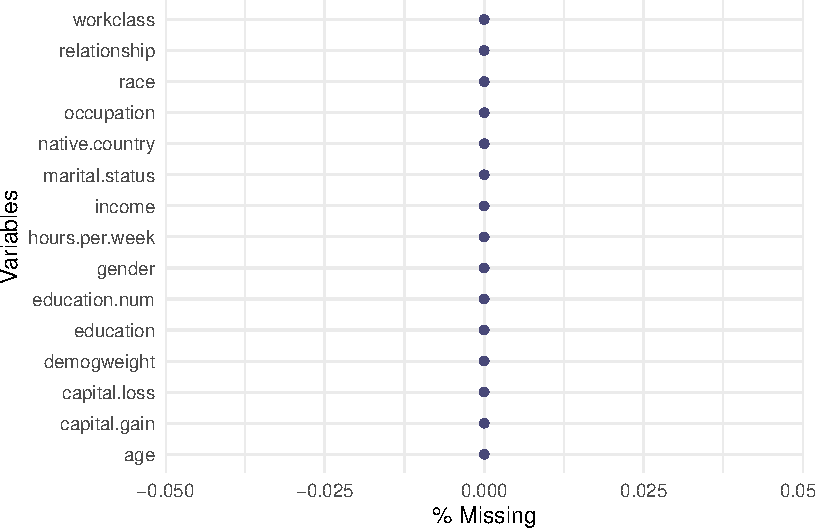
\includegraphics[width=0.6\linewidth,height=\textheight,keepaspectratio]{3-Data-preparation_files/figure-pdf/unnamed-chunk-22-1.pdf}
\end{center}

The resulting plot confirms that only three variables contain missing
values: \texttt{workclass} with 2794 entries, \texttt{occupation} with
2804 entries, and \texttt{native.country} with 847 entries.

Since the proportion of missing values is small, less than 0.06\% in
each case, we choose to impute the missing values rather than remove
rows, which could lead to information loss. To preserve each variable's
distribution, we use \emph{random imputation}, which replaces missing
entries by randomly sampling from observed (non-missing) values:

\begin{Shaded}
\begin{Highlighting}[]
\FunctionTok{library}\NormalTok{(Hmisc)}

\NormalTok{adult}\SpecialCharTok{$}\NormalTok{workclass      }\OtherTok{\textless{}{-}} \FunctionTok{impute}\NormalTok{(adult}\SpecialCharTok{$}\NormalTok{workclass,      }\StringTok{"random"}\NormalTok{)}
\NormalTok{adult}\SpecialCharTok{$}\NormalTok{native.country }\OtherTok{\textless{}{-}} \FunctionTok{impute}\NormalTok{(adult}\SpecialCharTok{$}\NormalTok{native.country, }\StringTok{"random"}\NormalTok{)}
\NormalTok{adult}\SpecialCharTok{$}\NormalTok{occupation     }\OtherTok{\textless{}{-}} \FunctionTok{impute}\NormalTok{(adult}\SpecialCharTok{$}\NormalTok{occupation,     }\StringTok{"random"}\NormalTok{)}
\end{Highlighting}
\end{Shaded}

Finally, we recheck for missingness to confirm that the imputation
succeeded:

\begin{Shaded}
\begin{Highlighting}[]
\FunctionTok{gg\_miss\_var}\NormalTok{(adult, }\AttributeTok{show\_pct =} \ConstantTok{TRUE}\NormalTok{)}
\end{Highlighting}
\end{Shaded}

\begin{center}
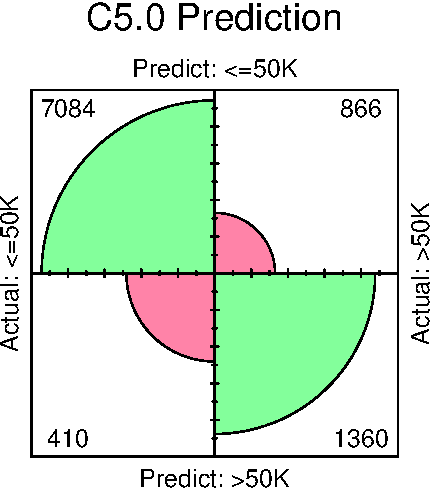
\includegraphics[width=0.6\linewidth,height=\textheight,keepaspectratio]{3-Data-preparation_files/figure-pdf/unnamed-chunk-24-1.pdf}
\end{center}

The updated plot should confirm that all missing values have been
addressed. With this step complete, we are ready to encode categorical
variables and scale numerical features, two more critical tasks in
preparing the dataset for modeling.

\subsection{Encoding Categorical
Variables}\label{encoding-categorical-variables}

Categorical variables often contain many unique values, which can
complicate modeling and lead to overfitting if not handled carefully. In
the \emph{adult} dataset, two features, \texttt{native.country} and
\texttt{workclass}, have a relatively high number of categories. To
simplify modeling while preserving interpretability, we group related
categories into broader, more informative classes.

\subsubsection*{\texorpdfstring{Grouping \texttt{native.country} by
Region}{Grouping native.country by Region}}\label{grouping-native.country-by-region}
\addcontentsline{toc}{subsubsection}{Grouping \texttt{native.country} by
Region}

The \texttt{native.country} variable includes 40 distinct countries.
Modeling each country as a separate category would unnecessarily expand
the feature space and dilute predictive power. To improve
interpretability and reduce sparsity, we group the countries into
broader geographic regions that reflect cultural and linguistic
proximity:

\begin{itemize}
\item
  \emph{Europe:} France, Germany, Greece, Hungary, Ireland, Italy,
  Netherlands, Poland, Portugal, United Kingdom, Yugoslavia.
\item
  \emph{North America:} United States, Canada, Outlying US territories
  (Guam, US Virgin Islands, etc.).
\item
  \emph{Latin America:} Mexico, El Salvador, Guatemala, Honduras,
  Nicaragua, Cuba, Dominican Republic, Puerto Rico, Colombia, Ecuador,
  Peru.
\item
  \emph{Caribbean:} Jamaica, Haiti, Trinidad and Tobago.
\item
  \emph{Asia:} Cambodia, China, Hong Kong, India, Iran, Japan, Laos,
  Philippines, South Korea (recorded as ``South'' in the dataset),
  Taiwan, Thailand, Vietnam.
\end{itemize}

The reclassification is performed using the \texttt{fct\_collapse()}
function from the \textbf{forcats} package. This function is designed
for factor manipulation and allows you to combine multiple existing
levels into broader, user-defined categories. It takes a factor variable
as input and a set of named groups, where each name defines a new level
and the associated vector lists the original levels to be merged. This
approach keeps the factor variable tidy and avoids manual recoding.

\begin{Shaded}
\begin{Highlighting}[]
\FunctionTok{library}\NormalTok{(forcats)}

\NormalTok{Europe }\OtherTok{\textless{}{-}} \FunctionTok{c}\NormalTok{(}\StringTok{"France"}\NormalTok{, }\StringTok{"Germany"}\NormalTok{, }\StringTok{"Greece"}\NormalTok{, }\StringTok{"Hungary"}\NormalTok{, }\StringTok{"Ireland"}\NormalTok{, }\StringTok{"Italy"}\NormalTok{, }\StringTok{"Netherlands"}\NormalTok{, }\StringTok{"Poland"}\NormalTok{, }\StringTok{"Portugal"}\NormalTok{, }\StringTok{"United{-}Kingdom"}\NormalTok{, }\StringTok{"Yugoslavia"}\NormalTok{)}

\NormalTok{North\_America }\OtherTok{\textless{}{-}} \FunctionTok{c}\NormalTok{(}\StringTok{"United{-}States"}\NormalTok{, }\StringTok{"Canada"}\NormalTok{, }\StringTok{"Outlying{-}US(Guam{-}USVI{-}etc)"}\NormalTok{)}

\NormalTok{Latin\_America }\OtherTok{\textless{}{-}} \FunctionTok{c}\NormalTok{(}\StringTok{"Mexico"}\NormalTok{, }\StringTok{"El{-}Salvador"}\NormalTok{, }\StringTok{"Guatemala"}\NormalTok{, }\StringTok{"Honduras"}\NormalTok{, }\StringTok{"Nicaragua"}\NormalTok{, }\StringTok{"Cuba"}\NormalTok{, }\StringTok{"Dominican{-}Republic"}\NormalTok{, }\StringTok{"Puerto{-}Rico"}\NormalTok{, }\StringTok{"Colombia"}\NormalTok{, }\StringTok{"Ecuador"}\NormalTok{, }\StringTok{"Peru"}\NormalTok{)}

\NormalTok{Caribbean }\OtherTok{\textless{}{-}} \FunctionTok{c}\NormalTok{(}\StringTok{"Jamaica"}\NormalTok{, }\StringTok{"Haiti"}\NormalTok{, }\StringTok{"Trinidad\&Tobago"}\NormalTok{)}

\NormalTok{Asia }\OtherTok{\textless{}{-}} \FunctionTok{c}\NormalTok{(}\StringTok{"Cambodia"}\NormalTok{, }\StringTok{"China"}\NormalTok{, }\StringTok{"Hong{-}Kong"}\NormalTok{, }\StringTok{"India"}\NormalTok{, }\StringTok{"Iran"}\NormalTok{, }\StringTok{"Japan"}\NormalTok{, }\StringTok{"Laos"}\NormalTok{, }\StringTok{"Philippines"}\NormalTok{, }\StringTok{"South"}\NormalTok{, }\StringTok{"Taiwan"}\NormalTok{, }\StringTok{"Thailand"}\NormalTok{, }\StringTok{"Vietnam"}\NormalTok{)}

\NormalTok{adult}\SpecialCharTok{$}\NormalTok{native.country }\OtherTok{\textless{}{-}} \FunctionTok{fct\_collapse}\NormalTok{(adult}\SpecialCharTok{$}\NormalTok{native.country,}
        \StringTok{"Europe"}        \OtherTok{=}\NormalTok{ Europe,}
        \StringTok{"North America"} \OtherTok{=}\NormalTok{ North\_America,}
        \StringTok{"Latin America"} \OtherTok{=}\NormalTok{ Latin\_America,}
        \StringTok{"Caribbean"}     \OtherTok{=}\NormalTok{ Caribbean,}
        \StringTok{"Asia"}          \OtherTok{=}\NormalTok{ Asia}
\NormalTok{)}
\end{Highlighting}
\end{Shaded}

To verify the transformation:

\begin{Shaded}
\begin{Highlighting}[]
\FunctionTok{table}\NormalTok{(adult}\SpecialCharTok{$}\NormalTok{native.country)}
   
\NormalTok{            Asia North America Latin America        Europe     Caribbean }
            \DecValTok{1108}         \DecValTok{44582}          \DecValTok{1899}           \DecValTok{797}           \DecValTok{212}
\end{Highlighting}
\end{Shaded}

This regional grouping provides a balance between detail and
interpretability. It retains key cultural and geographic distinctions
(for example, between Latin America and the Caribbean) while minimizing
sparsity and reducing the risk of overfitting when the variable is used
in predictive modeling.

\subsubsection*{\texorpdfstring{Simplifying
\texttt{workclass}}{Simplifying workclass}}\label{simplifying-workclass}
\addcontentsline{toc}{subsubsection}{Simplifying \texttt{workclass}}

The \texttt{workclass} variable categorizes employment types. Two of its
levels, ``Never-worked'' and ``Without-pay'', are rare and similar in
nature, representing individuals outside formal employment. We
consolidate these under a single label: \texttt{Unemployed}.

\begin{Shaded}
\begin{Highlighting}[]
\NormalTok{adult}\SpecialCharTok{$}\NormalTok{workclass }\OtherTok{\textless{}{-}} \FunctionTok{fct\_collapse}\NormalTok{(adult}\SpecialCharTok{$}\NormalTok{workclass, }\StringTok{"Unemployed"} \OtherTok{=} \FunctionTok{c}\NormalTok{(}\StringTok{"Never{-}worked"}\NormalTok{, }\StringTok{"Without{-}pay"}\NormalTok{))}
\end{Highlighting}
\end{Shaded}

To confirm the update:

\begin{Shaded}
\begin{Highlighting}[]
\FunctionTok{table}\NormalTok{(adult}\SpecialCharTok{$}\NormalTok{workclass)}
   
\NormalTok{          Gov Unemployed    Private   Self}\SpecialCharTok{{-}}\NormalTok{emp }
         \DecValTok{6919}         \DecValTok{32}      \DecValTok{35851}       \DecValTok{5796}
\end{Highlighting}
\end{Shaded}

By reducing the number of categories in \texttt{workclass} and
\texttt{native.country}, we streamline the dataset while retaining
interpretability. This prepares the data for modeling algorithms that
are sensitive to high-cardinality categorical inputs.

\subsection{Handling Outliers}\label{handling-outliers}

Identifying and addressing outliers is an important part of data
preparation. Extreme values can distort summary statistics and influence
the performance of models, particularly those sensitive to the range of
numeric features. In this section, we focus on the \texttt{capital.loss}
variable from the \emph{adult} dataset to examine whether outliers are
present and how they should be handled.

We begin with a basic summary:

\begin{Shaded}
\begin{Highlighting}[]
\FunctionTok{summary}\NormalTok{(adult}\SpecialCharTok{$}\NormalTok{capital.loss)}
\NormalTok{      Min. }\DecValTok{1}\NormalTok{st Qu.  Median    Mean }\DecValTok{3}\NormalTok{rd Qu.    Max. }
      \FloatTok{0.00}    \FloatTok{0.00}    \FloatTok{0.00}   \FloatTok{87.94}    \FloatTok{0.00} \FloatTok{4356.00}
\end{Highlighting}
\end{Shaded}

From this output, we observe that the minimum value is 0, and the
maximum is 4356. A majority of observations, over 75\%, have a value of
0. The median, 0, is substantially lower than the mean, 87.94,
indicating a right-skewed distribution influenced by high values.

To explore this further, we visualize the distribution using both a
boxplot and a histogram:

\begin{Shaded}
\begin{Highlighting}[]
\FunctionTok{ggplot}\NormalTok{(}\AttributeTok{data =}\NormalTok{ adult, }\FunctionTok{aes}\NormalTok{(}\AttributeTok{y =}\NormalTok{ capital.loss)) }\SpecialCharTok{+}
     \FunctionTok{geom\_boxplot}\NormalTok{(}\AttributeTok{color =} \StringTok{"\#377EB8"}\NormalTok{, }\AttributeTok{fill =} \StringTok{"\#e5f4fb"}\NormalTok{) }\SpecialCharTok{+}
     \FunctionTok{ggtitle}\NormalTok{(}\StringTok{"Boxplot of Capital Loss"}\NormalTok{)}

\FunctionTok{ggplot}\NormalTok{(}\AttributeTok{data =}\NormalTok{ adult, }\FunctionTok{aes}\NormalTok{(}\AttributeTok{x =}\NormalTok{ capital.loss)) }\SpecialCharTok{+}
     \FunctionTok{geom\_histogram}\NormalTok{(}\AttributeTok{bins =} \DecValTok{30}\NormalTok{, }\AttributeTok{color =} \StringTok{"white"}\NormalTok{, }\AttributeTok{fill =} \StringTok{"\#2C7BB6"}\NormalTok{) }\SpecialCharTok{+}
     \FunctionTok{ggtitle}\NormalTok{(}\StringTok{"Histogram of Capital Loss"}\NormalTok{)}
\end{Highlighting}
\end{Shaded}

\begin{figure}

\begin{minipage}{0.50\linewidth}
\begin{center}
\pandocbounded{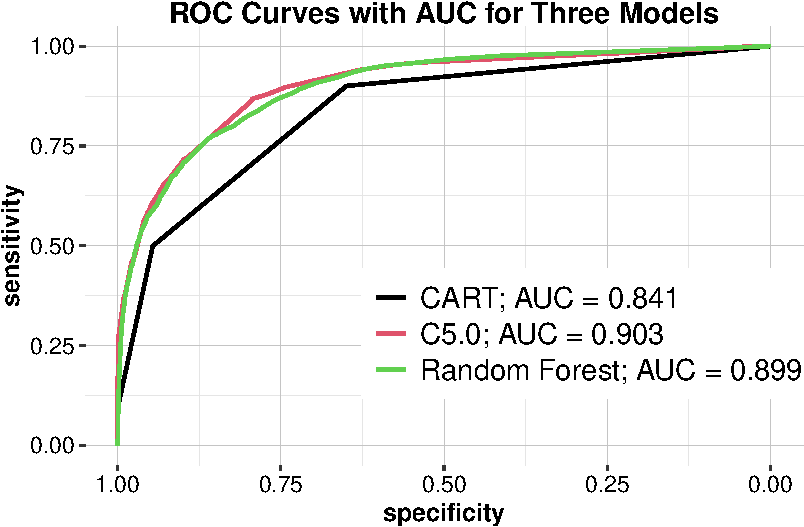
\includegraphics[keepaspectratio]{3-Data-preparation_files/figure-pdf/unnamed-chunk-30-1.pdf}}
\end{center}
\end{minipage}%
%
\begin{minipage}{0.50\linewidth}
\begin{center}
\pandocbounded{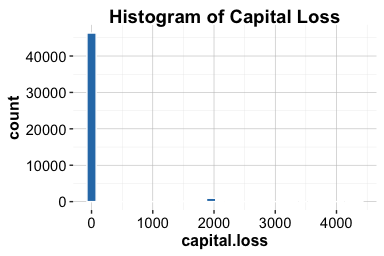
\includegraphics[keepaspectratio]{3-Data-preparation_files/figure-pdf/unnamed-chunk-30-2.pdf}}
\end{center}
\end{minipage}%

\end{figure}%

The boxplot shows a strong positive skew, with several high values
extending beyond the upper whisker. The histogram confirms that most
individuals report zero capital loss, with a few concentrated peaks near
2,000 and 4,000.

To focus more closely on the nonzero values, we restrict our analysis to
rows where \texttt{capital.loss\ \textgreater{}\ 0}:

\begin{Shaded}
\begin{Highlighting}[]
\NormalTok{subset\_adult }\OtherTok{\textless{}{-}} \FunctionTok{subset}\NormalTok{(adult, capital.loss }\SpecialCharTok{\textgreater{}} \DecValTok{0}\NormalTok{)}

\FunctionTok{ggplot}\NormalTok{(}\AttributeTok{data =}\NormalTok{ subset\_adult, }\FunctionTok{aes}\NormalTok{(}\AttributeTok{y =}\NormalTok{ capital.loss)) }\SpecialCharTok{+}
     \FunctionTok{geom\_boxplot}\NormalTok{(}\AttributeTok{color =} \StringTok{"\#377EB8"}\NormalTok{, }\AttributeTok{fill =} \StringTok{"\#e5f4fb"}\NormalTok{) }\SpecialCharTok{+}
     \FunctionTok{ggtitle}\NormalTok{(}\StringTok{"Boxplot of Nonzero Capital Loss"}\NormalTok{)}

\FunctionTok{ggplot}\NormalTok{(}\AttributeTok{data =}\NormalTok{ subset\_adult, }\FunctionTok{aes}\NormalTok{(}\AttributeTok{x =}\NormalTok{ capital.loss)) }\SpecialCharTok{+}
     \FunctionTok{geom\_histogram}\NormalTok{(}\AttributeTok{bins =} \DecValTok{30}\NormalTok{, }\AttributeTok{color =} \StringTok{"white"}\NormalTok{, }\AttributeTok{fill =} \StringTok{"\#2C7BB6"}\NormalTok{) }\SpecialCharTok{+}
     \FunctionTok{ggtitle}\NormalTok{(}\StringTok{"Histogram of Nonzero Capital Loss"}\NormalTok{)}
\end{Highlighting}
\end{Shaded}

\begin{figure}

\begin{minipage}{0.50\linewidth}
\begin{center}
\pandocbounded{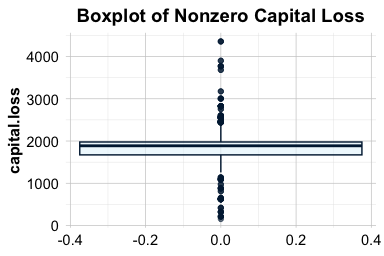
\includegraphics[keepaspectratio]{3-Data-preparation_files/figure-pdf/unnamed-chunk-31-1.pdf}}
\end{center}
\end{minipage}%
%
\begin{minipage}{0.50\linewidth}
\begin{center}
\pandocbounded{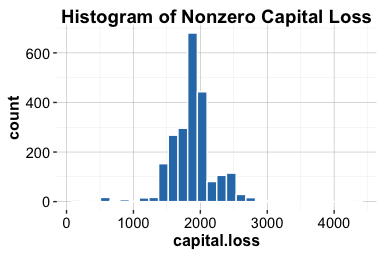
\includegraphics[keepaspectratio]{3-Data-preparation_files/figure-pdf/unnamed-chunk-31-2.pdf}}
\end{center}
\end{minipage}%

\end{figure}%

Among those with a nonzero capital loss, the majority of values are
concentrated below 500. However, a small number of observations exceed
4,000. Despite their rarity, these high values appear to follow a
relatively smooth and symmetric distribution, suggesting they reflect
genuine variation in the data rather than data entry errors.

Given this context, we choose to retain the extreme values in
\texttt{capital.loss}. They are likely to reflect meaningful differences
across individuals and should not be removed without strong
justification. If we later find that these values introduce problems for
modeling, we may consider one of several strategies: applying a log or
square-root transformation to reduce skewness, creating a binary
variable to indicate whether a capital loss occurred, or using
winsorization to cap extreme values at a defined threshold.

Understanding the structure of \texttt{capital.loss} also prepares us
for handling the related variable \texttt{capital.gain}, which we
explore next. For a hands-on example, see the guided exercise at the end
of this chapter.

\section{Chapter Summary and
Takeaways}\label{chapter-summary-and-takeaways-2}

This chapter covered the essential steps of data preparation, showing
how to transform raw data into a format suitable for analysis. Using the
\emph{diamonds} and \emph{adult} datasets, we practiced identifying
outliers, handling missing values, scaling numerical features, and
encoding categorical variables.

We emphasized that data preparation is not just technical; it is driven
by the structure and meaning of each feature. Outliers can distort
results, missing values must be addressed carefully, and categorical
variables require appropriate encoding. Scaling ensures fairness across
features for many algorithms.

These techniques, though often overlooked, are crucial for building
reliable and interpretable models. Clean, well-structured data forms the
foundation of every successful data science project.

Next chapter, we move to exploratory data analysis, where we begin
uncovering patterns and relationships that inform our modeling choices.

\section{Exercises}\label{sec-ch3-exercises}

This section includes exercises designed to deepen your understanding of
data preparation. They cover conceptual questions, hands-on practice
with the \emph{diamonds} and \emph{adult} datasets, and reflection on
ethical and real-world issues. These exercises can be completed in R and
build on the examples discussed in this chapter.

\subsubsection*{Understanding Data
Types}\label{understanding-data-types}
\addcontentsline{toc}{subsubsection}{Understanding Data Types}

\begin{enumerate}
\def\labelenumi{\arabic{enumi}.}
\item
  Explain the difference between continuous and discrete numerical
  variables, and give a real-world example of each.
\item
  How do ordinal and nominal categorical variables differ? Provide one
  example for each type.
\item
  Use the \texttt{typeof()} and \texttt{class()} functions in R to
  investigate how numerical and categorical variables are represented
  internally.
\item
  Why is it important to identify the correct data types before
  modeling?
\end{enumerate}

\subsubsection*{Working with the Diamonds
Dataset}\label{working-with-the-diamonds-dataset}
\addcontentsline{toc}{subsubsection}{Working with the Diamonds Dataset}

\begin{enumerate}
\def\labelenumi{\arabic{enumi}.}
\setcounter{enumi}{4}
\item
  Use \texttt{summary()} to inspect the \emph{diamonds} dataset. What
  patterns or irregularities do you notice?
\item
  Classify the variables in the \emph{diamonds} dataset as numerical,
  ordinal, or nominal.
\item
  Create histograms of \texttt{carat} and \texttt{price}. Describe their
  distributions and note any skewness or gaps.
\end{enumerate}

\subsubsection*{Detecting and Treating
Outliers}\label{detecting-and-treating-outliers}
\addcontentsline{toc}{subsubsection}{Detecting and Treating Outliers}

\begin{enumerate}
\def\labelenumi{\arabic{enumi}.}
\setcounter{enumi}{7}
\item
  Identify outliers in the \texttt{x} variable using boxplots and
  histograms. If outliers are found, apply a method to handle them as
  done for \texttt{y} in Section \ref{sec-ch3-data-pre-outliers}.
\item
  Repeat the process for the \texttt{z} variable and comment on the
  results.
\item
  Examine the \texttt{depth} variable. What method would you use to
  detect and treat outliers in this case?
\item
  Discuss the pros and cons of removing outliers versus applying a
  transformation. Use examples from this chapter to support your answer.
\end{enumerate}

\subsubsection*{Encoding Categorical
Variables}\label{encoding-categorical-variables-1}
\addcontentsline{toc}{subsubsection}{Encoding Categorical Variables}

\begin{enumerate}
\def\labelenumi{\arabic{enumi}.}
\setcounter{enumi}{11}
\item
  Show how to apply ordinal encoding to the \texttt{cut} variable in the
  \emph{diamonds} dataset.
\item
  Demonstrate one-hot encoding for the \texttt{color} variable using
  appropriate R functions.
\item
  What problems can arise when applying ordinal encoding to a nominal
  variable?
\item
  Under what conditions is frequency encoding more appropriate than
  one-hot encoding?
\end{enumerate}

\subsubsection*{Exploring the Adult
Dataset}\label{exploring-the-adult-dataset}
\addcontentsline{toc}{subsubsection}{Exploring the Adult Dataset}

\begin{enumerate}
\def\labelenumi{\arabic{enumi}.}
\setcounter{enumi}{15}
\item
  Load the \emph{adult} dataset from the \textbf{liver} package and
  classify its categorical variables as nominal or ordinal.
\item
  Compute the proportion of individuals earning more than \$50K. What
  does this tell you about income distribution?
\item
  Generate a boxplot and histogram of \texttt{capital.gain}. What
  insights or anomalies can you identify?
\item
  Are there any outliers in \texttt{capital.gain}? If so, suggest how
  you would handle them.
\item
  Create a correlation matrix for the numerical variables. What do the
  correlations reveal about the relationships between features?
\end{enumerate}

\subsubsection*{Feature Engineering and
Scaling}\label{feature-engineering-and-scaling}
\addcontentsline{toc}{subsubsection}{Feature Engineering and Scaling}

\begin{enumerate}
\def\labelenumi{\arabic{enumi}.}
\setcounter{enumi}{20}
\item
  Use the \texttt{cut()} function to group \texttt{age} into three
  categories: Young (\(\le 30\)), Middle-aged (31--50), and Senior
  (\(>50\)). Name the new variable \texttt{Age\_Group}.
\item
  Calculate the mean \texttt{capital.gain} for each \texttt{Age\_Group}.
  What does this reveal?
\item
  Create a binary variable indicating whether an individual has nonzero
  \texttt{capital.gain}, and use it to create an exploratory plot.
\item
  Group the 16 education levels into broader categories using
  \texttt{fct\_collapse()}. Propose at least three meaningful groupings.
\item
  Define a new variable \texttt{net.capital} as the difference between
  \texttt{capital.gain} and \texttt{capital.loss}. Analyze its
  distribution using plots.
\item
  Apply min-max scaling to \texttt{age}, \texttt{capital.gain},
  \texttt{capital.loss}, and \texttt{hours.per.week} using
  \texttt{mutate()} and summarize the results.
\item
  Apply z-score scaling to the same variables. How do the results
  compare to min-max scaling?
\end{enumerate}

\subsubsection*{Modeling and Real-World
Scenarios}\label{modeling-and-real-world-scenarios}
\addcontentsline{toc}{subsubsection}{Modeling and Real-World Scenarios}

\begin{enumerate}
\def\labelenumi{\arabic{enumi}.}
\setcounter{enumi}{27}
\item
  If you were designing a credit scoring system, how would you encode
  features like \texttt{employment.type} or \texttt{loan.purpose}?
\item
  In a dataset where 25\% of income values are missing, which imputation
  strategy would you use, and why?
\item
  A customer satisfaction variable includes five levels from ``Very
  satisfied'' to ``Very dissatisfied.'' Which encoding method is most
  appropriate, and why?
\item
  Would you handle outliers in patient temperature data differently than
  outliers in income data? Explain your reasoning.
\end{enumerate}

\subsubsection*{Ethics and Reflection}\label{ethics-and-reflection}
\addcontentsline{toc}{subsubsection}{Ethics and Reflection}

\begin{enumerate}
\def\labelenumi{\arabic{enumi}.}
\setcounter{enumi}{31}
\item
  What ethical concerns might arise from dropping rows with missing
  data, particularly for underrepresented groups?
\item
  How can careless encoding of categorical variables lead to biased or
  unfair model outcomes? Provide an example.
\item
  A model performs well in training but poorly in production. How might
  decisions made during data preparation explain this discrepancy?
\item
  Reflect on a dataset you have worked with (or the \emph{housePrice}
  dataset from the \textbf{liver} package). Which data preparation steps
  would you revise based on the techniques from this chapter?
\end{enumerate}

\bookmarksetup{startatroot}

\chapter{Exploratory Data Analysis}\label{sec-ch4-EDA}

Exploratory Data Analysis (EDA) is the essential first step before
building models or conducting statistical inference. It involves
examining data carefully, thoroughly, and creatively to uncover
insights. EDA helps reveal unexpected patterns, spot anomalies, and
highlight relationships that shape the direction of further analysis.

EDA plays a pivotal role in the Data Science Workflow (see
Figure~\ref{fig-ch2_DSW}), functioning as the bridge between Data
Preparation (Chapter \ref{sec-ch3-data-preparation}) and (Chapter
\ref{sec-ch6-setup-data}). This phase deepens our understanding of the
data's structure, quality, and potential, ensuring that downstream
decisions rest on a solid foundation.

Unlike formal hypothesis testing, EDA is not rigid or sequential. It is
an iterative, open-ended process that invites curiosity. Different
datasets pose different questions. Some exploratory paths reveal
meaningful trends, while others point to data issues or dead ends.
Through iterative exploration, analysts develop intuition and refine
their focus, ultimately identifying the most informative features for
modeling.

The primary aim of EDA is not to confirm theories, but to generate
insight. Summary statistics, exploratory visualizations, and correlation
measures offer an initial map of the data landscape. Such exploratory
findings must be interpreted with caution, as they are preliminary and
may not reflect causal relationships. Later chapters, particularly
Chapter \ref{sec-ch5-statistics}, will introduce formal tools for
inference and prediction.

EDA also emphasizes the importance of \emph{practical relevance}. In
large datasets, even weak patterns can be statistically significant but
lack real-world utility. For example, a weak correlation between
customer engagement and churn may appear significant due to sample size,
yet offer little actionable value. Integrating domain knowledge is
essential for interpreting such findings.

Finally, EDA is closely tied to data quality. Outliers, missing values,
inconsistent formats, and redundant variables often come to light during
exploration. Addressing these issues early is critical for building
effective and trustworthy models. The choice of EDA techniques depends
on both the characteristics of the data and the analytical questions at
hand. Histograms and box plots reveal distributions; scatter plots and
correlation matrices highlight relationships. The next sections
introduce these tools in context and explain how to apply them
effectively.

\subsection*{What This Chapter Covers}\label{what-this-chapter-covers-3}
\addcontentsline{toc}{subsection}{What This Chapter Covers}

This chapter introduces EDA as a critical phase in the data science
workflow. You will learn how to apply summary statistics and visual
techniques to examine variable distributions, detect anomalies, and
uncover relationships that inform downstream modeling. In addition, you
will explore how correlation analysis can identify redundancy and how
multivariate patterns contribute to predictive insight.

We begin with two foundational sections: \emph{Key Objectives and
Guiding Questions for EDA}, which frame the exploratory mindset, and
\emph{EDA as Data Storytelling}, which emphasizes the importance of
communicating insights clearly and effectively.

Following these conceptual foundations, we walk you through a guided EDA
of the \emph{churn} dataset. You will explore how real-world patterns
emerge from the data, how visualizations reveal customer behavior, and
how these insights prepare the ground for classification modeling using
k-nearest neighbors in Chapter \ref{sec-ch7-classification-knn}.

The chapter concludes with hands-on exercises and a guided project using
the \emph{bank} dataset. This project offers further opportunities to
practice EDA techniques and lays the foundation for the neural network
case study presented in Chapter \ref{sec-ch12-neural-networks}.

\section{Objectives and Guiding Questions for
EDA}\label{sec-EDA-objectives-questions}

EDA marks the first substantive interaction between analyst and dataset,
the moment when raw data begins to reveal its structure, surprises, and
potential narratives. Rather than rushing into modeling, experienced
data scientists pause to ask: \emph{What is in the data? What patterns
stand out? What problems need attention?}

Before applying specific techniques, it is helpful to clarify what EDA
is designed to accomplish. At its core, EDA aims to:

\begin{itemize}
\item
  \emph{Identify the structure of the data} -- Detect variable types,
  value ranges, missing entries, and potential anomalies.
\item
  \emph{Examine variable distributions} -- Assess spread, skewness, and
  central tendency for numerical and categorical features.
\item
  \emph{Investigate relationships between variables} -- Uncover
  associations, dependencies, or interactions that may inform
  predictions.
\item
  \emph{Detect patterns and outliers} -- Spot unusual values or
  subgroups that could indicate errors, or hidden signals.
\end{itemize}

Together, these objectives provide a foundation for effective modeling.
They help analysts refine feature choices, anticipate modeling
challenges, and surface early insights worth pursuing.

EDA becomes even more powerful when guided by focused questions. These
typically fall into two broad categories: \emph{univariate analysis},
which examines variables individually, and \emph{multivariate analysis},
which explores their relationships.

\textbf{Univariate analysis} asks: What does each variable reveal on its
own? This includes inspecting distributions, central tendencies, and
variability, as well as checking for missing values or irregularities.
Common questions include:

\begin{itemize}
\item
  What is the distribution of the target variable?
\item
  How are numerical features, such as income or age, distributed?
\item
  Are there missing values, and do they follow a specific pattern?
\end{itemize}

Histograms, box plots, and summary statistics (mean, median, quartiles,
standard deviation) are essential tools at this stage.

\textbf{Multivariate analysis} shifts the focus to interactions among
variables. It uncovers dependencies, correlations, or redundancies that
may affect modeling. Key questions include:

\begin{itemize}
\item
  How does the target variable relate to its predictors?
\item
  Are any predictors highly correlated, raising concerns about
  multicollinearity?
\item
  How do categorical and numerical features interact?
\end{itemize}

Scatter plots, grouped visualizations, and correlation matrices help
reveal these patterns and guide thoughtful feature selection.

One recurring challenge in EDA, especially for students, is deciding
which plots or techniques are best suited to different types of data and
questions. Table \ref{tbl-EDA-table-tools} offers a concise mapping of
exploratory objectives to effective tools. It serves as a practical
reference to support informed, purposeful analysis.

\begin{table}

\caption{\label{tbl-EDA-table-tools}Overview of Recommended Tools for
Common EDA Objectives.}

\centering{

\centering
\begin{tabular}[t]{>{\raggedright\arraybackslash}p{12em}>{\raggedright\arraybackslash}p{11em}>{\raggedright\arraybackslash}p{13em}}
\toprule
Exploratory.Objective & Applicable.Data.Type & Recommended.Techniques\\
\midrule
Examine a variable’s distribution & Numerical & Histogram, box plot, density plot, summary statistics\\
Summarize a categorical variable & Categorical & Bar chart, frequency table\\
Identify outliers & Numerical & Box plot, histogram\\
Detect missing data patterns & Any & Summary statistics, missingness maps\\
Explore the relationship between two numerical variables & Numerical \& Numerical & Scatter plot, correlation coefficient\\
\addlinespace
Compare a numerical variable across groups & Numerical \& Categorical & Box plot, grouped bar chart, violin plot\\
Analyze interactions between two categorical variables & Categorical \& Categorical & Stacked bar chart, mosaic plot, contingency table\\
Assess correlation among multiple numerical variables & Multiple Numerical & Correlation matrix, scatterplot matrix\\
\bottomrule
\end{tabular}

}

\end{table}%

By aligning key objectives with guiding questions and appropriate
methods, EDA becomes more than an exploratory routine, it becomes a
strategic component of the data science workflow. It improves data
quality, informs feature design, and lays the foundation for effective
modeling.

In the next section, we turn to the role of storytelling in EDA and
explore how visual and narrative techniques can make exploratory
insights more accessible and impactful.

\section{EDA as Data Storytelling}\label{eda-as-data-storytelling}

Exploratory Data Analysis is not only a technical process for uncovering
patterns, it is also a means of communicating insights clearly and
persuasively. While EDA reveals structure, anomalies, and relationships,
these findings become valuable only when they are communicated with
clarity and purpose. This is where data storytelling becomes essential:
it transforms exploration into insight.

Effective storytelling in data science weaves together analytical
evidence, contextual knowledge, and visual clarity. Rather than
presenting statistics or charts in isolation, strong EDA links each
observation to a broader narrative. Whether the audience includes fellow
analysts, business stakeholders, or policymakers, the goal remains the
same: to convey insights in ways that are meaningful and relevant.

Consider a typical finding: customers with high daytime usage are more
likely to churn. Stating this fact is informative, but incomplete. A
compelling narrative connects the pattern to its implication:

\emph{``Customers with extensive daytime usage are significantly more
likely to churn, possibly due to pricing concerns or dissatisfaction
with service quality. Targeted retention strategies, such as customized
discounts or flexible pricing plans, may help mitigate this risk.''}

This shift from raw description to interpretation is at the heart of
data storytelling. It invites action and supports informed
decision-making.

Visualizations play a central role in this process. While summary
statistics provide a structural overview, visual displays make patterns
tangible. Scatter plots and correlation matrices reveal relationships
among numerical features; histograms and box plots clarify distributions
and skewness; bar charts and stacked visuals enable comparisons across
categories. Selecting the right visual tool enhances both understanding
and communication.

Data storytelling is now common across domains, from business and
journalism to public policy and scientific research. A well-known
example appears in Hans Rosling's TED Talk
\href{https://www.ted.com/talks/hans_rosling_new_insights_on_poverty}{``New
insights on poverty''}. Figure Figure~\ref{fig-EDA-fig-1}, adapted from
his presentation, illustrates how GDP per capita and life expectancy
have changed across global regions from 1962 to 2011. It presents
decades of demographic and health data into an engaging and
comprehensible format. Although this example is drawn from global
development, the same principles apply when exploring customer behavior,
financial trends, or healthcare outcomes.

\begin{figure}[H]

\centering{

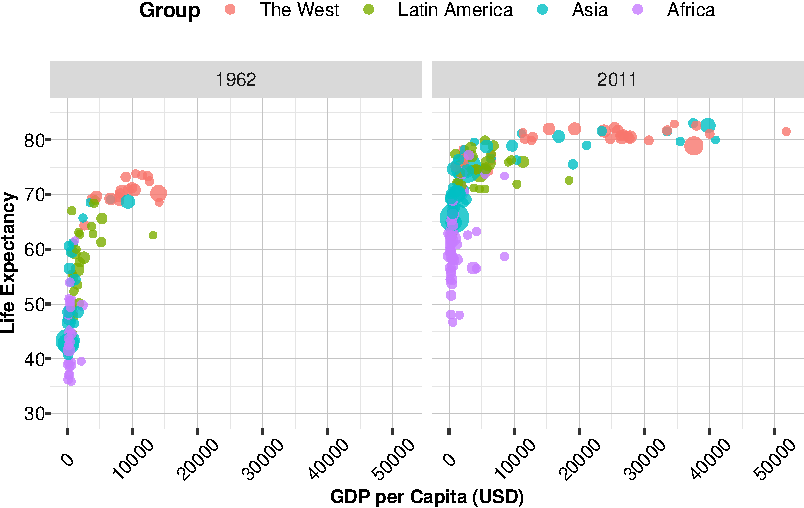
\includegraphics[width=1\linewidth,height=\textheight,keepaspectratio]{4-Exploratory-data-analysis_files/figure-pdf/fig-EDA-fig-1-1.pdf}

}

\caption{\label{fig-EDA-fig-1}Changes in GDP per capita and life
expectancy by region from 1962 to 2011. Dot size is proportional to
population.}

\end{figure}%

As you conduct EDA, it is worth asking not only \emph{what} the data
shows, but also \emph{why} those patterns matter. What story is
emerging? How can that story inform a decision, challenge an assumption,
or inspire further analysis? Framing EDA as storytelling ensures that
exploratory work is not merely descriptive but purposeful, anchored in
the real-world questions that motivated the analysis in the first place.

To illustrate these principles in practice, the next section walks
through a detailed EDA of customer churn, demonstrating how statistical
summaries, visual tools, and domain reasoning can uncover meaningful
patterns that guide predictive modeling.

\section{\texorpdfstring{EDA in Practice: The \emph{Churn}
Dataset}{EDA in Practice: The Churn Dataset}}\label{sec-ch4-EDA-churn}

EDA is most effective when applied to real data with real questions. In
this section, we demonstrate how to conduct EDA using the \emph{churn}
dataset, which contains behavioral and demographic information about
customers---along with a binary outcome indicating whether each customer
has churned (i.e., discontinued the service).

This walkthrough follows the structure of the Data Science Workflow
introduced in Chapter \ref{sec-ch2-intro-data-science}. We begin by
briefly revisiting the first two steps, \emph{Problem Understanding} and
\emph{Data Understanding}, to set the business context and examine the
structure of the dataset. The main emphasis here is on \emph{Step 3:
Exploratory Data Analysis}, where we use summary statistics,
visualizations, and guiding questions to uncover meaningful patterns
related to customer churn.

The insights developed in this section serve as a springboard for the
next phases of analysis: preparing the data for modeling in Chapter
\ref{sec-ch6-setup-data}, building predictive models using k-Nearest
Neighbors in Chapter \ref{sec-ch7-classification-knn}, and evaluating
model performance in Chapter \ref{sec-ch8-evaluation}. By working
through these steps in sequence, you will see how a well-executed EDA
not only enhances understanding but also improves the quality of
decisions made through modeling.

\subsection*{Understanding the Churn
Problem}\label{understanding-the-churn-problem}
\addcontentsline{toc}{subsection}{Understanding the Churn Problem}

Customer churn (the loss of existing customers) is a central concern in
subscription-based industries such as telecommunications, finance, and
streaming services. Because retaining customers is typically more
cost-effective than acquiring new ones, identifying the drivers of churn
is a priority for both analysts and decision-makers.

From a business standpoint, this challenge prompts three key questions:

\begin{itemize}
\item
  \emph{Why} are customers deciding to leave?
\item
  \emph{What} behavioral or demographic patterns are associated with
  higher churn risk?
\item
  \emph{How} can these insights inform strategies to improve customer
  retention?
\end{itemize}

EDA provides the foundation for addressing these questions. By
identifying relevant patterns in the data, EDA uncovers potential
signals that can inform targeted interventions. It also helps frame the
predictive modeling task that follows.

In Chapter \ref{sec-ch7-classification-knn}, we will develop a k-nearest
neighbors (kNN) model to predict customer churn. Before building that
model, however, it is essential to understand the structure of the data,
the types of variables available, and the relationships they reveal.

\subsection*{\texorpdfstring{Overview of the \emph{churn}
Dataset}{Overview of the churn Dataset}}\label{overview-of-the-churn-dataset}
\addcontentsline{toc}{subsection}{Overview of the \emph{churn} Dataset}

Before diving into visualizations and summary statistics, it is
important to understand the dataset we will explore throughout this
chapter. The \emph{churn} dataset, included in the \textbf{liver}
package, provides a realistic example for practicing EDA. It includes
5,000 customer records across 20 variables, combining demographic
information, service usage, account attributes, and customer support
interactions.

The core variable of interest is \texttt{churn}, which indicates whether
a customer has left the service (\texttt{yes}) or remained
(\texttt{no}). This binary outcome will eventually serve as the target
for classification modeling in Chapter \ref{sec-ch7-classification-knn},
but our first task is to understand the data that surrounds it.

To load and inspect the dataset, run the following code in R:

\begin{Shaded}
\begin{Highlighting}[]
\FunctionTok{library}\NormalTok{(liver)}

\FunctionTok{data}\NormalTok{(churn)}
\FunctionTok{str}\NormalTok{(churn)}
   \StringTok{\textquotesingle{}data.frame\textquotesingle{}}\SpecialCharTok{:}    \DecValTok{5000}\NormalTok{ obs. of  }\DecValTok{20}\NormalTok{ variables}\SpecialCharTok{:}
    \ErrorTok{$}\NormalTok{ state         }\SpecialCharTok{:}\NormalTok{ Factor w}\SpecialCharTok{/} \DecValTok{51}\NormalTok{ levels }\StringTok{"AK"}\NormalTok{,}\StringTok{"AL"}\NormalTok{,}\StringTok{"AR"}\NormalTok{,..}\SpecialCharTok{:} \DecValTok{17} \DecValTok{36} \DecValTok{32} \DecValTok{36} \DecValTok{37} \DecValTok{2} \DecValTok{20} \DecValTok{25} \DecValTok{19} \DecValTok{50}\NormalTok{ ...}
    \SpecialCharTok{$}\NormalTok{ area.code     }\SpecialCharTok{:}\NormalTok{ Factor w}\SpecialCharTok{/} \DecValTok{3}\NormalTok{ levels }\StringTok{"area\_code\_408"}\NormalTok{,..}\SpecialCharTok{:} \DecValTok{2} \DecValTok{2} \DecValTok{2} \DecValTok{1} \DecValTok{2} \DecValTok{3} \DecValTok{3} \DecValTok{2} \DecValTok{1} \DecValTok{2}\NormalTok{ ...}
    \SpecialCharTok{$}\NormalTok{ account.length}\SpecialCharTok{:}\NormalTok{ int  }\DecValTok{128} \DecValTok{107} \DecValTok{137} \DecValTok{84} \DecValTok{75} \DecValTok{118} \DecValTok{121} \DecValTok{147} \DecValTok{117} \DecValTok{141}\NormalTok{ ...}
    \SpecialCharTok{$}\NormalTok{ voice.plan    }\SpecialCharTok{:}\NormalTok{ Factor w}\SpecialCharTok{/} \DecValTok{2}\NormalTok{ levels }\StringTok{"yes"}\NormalTok{,}\StringTok{"no"}\SpecialCharTok{:} \DecValTok{1} \DecValTok{1} \DecValTok{2} \DecValTok{2} \DecValTok{2} \DecValTok{2} \DecValTok{1} \DecValTok{2} \DecValTok{2} \DecValTok{1}\NormalTok{ ...}
    \SpecialCharTok{$}\NormalTok{ voice.messages}\SpecialCharTok{:}\NormalTok{ int  }\DecValTok{25} \DecValTok{26} \DecValTok{0} \DecValTok{0} \DecValTok{0} \DecValTok{0} \DecValTok{24} \DecValTok{0} \DecValTok{0} \DecValTok{37}\NormalTok{ ...}
    \SpecialCharTok{$}\NormalTok{ intl.plan     }\SpecialCharTok{:}\NormalTok{ Factor w}\SpecialCharTok{/} \DecValTok{2}\NormalTok{ levels }\StringTok{"yes"}\NormalTok{,}\StringTok{"no"}\SpecialCharTok{:} \DecValTok{2} \DecValTok{2} \DecValTok{2} \DecValTok{1} \DecValTok{1} \DecValTok{1} \DecValTok{2} \DecValTok{1} \DecValTok{2} \DecValTok{1}\NormalTok{ ...}
    \SpecialCharTok{$}\NormalTok{ intl.mins     }\SpecialCharTok{:}\NormalTok{ num  }\DecValTok{10} \FloatTok{13.7} \FloatTok{12.2} \FloatTok{6.6} \FloatTok{10.1} \FloatTok{6.3} \FloatTok{7.5} \FloatTok{7.1} \FloatTok{8.7} \FloatTok{11.2}\NormalTok{ ...}
    \SpecialCharTok{$}\NormalTok{ intl.calls    }\SpecialCharTok{:}\NormalTok{ int  }\DecValTok{3} \DecValTok{3} \DecValTok{5} \DecValTok{7} \DecValTok{3} \DecValTok{6} \DecValTok{7} \DecValTok{6} \DecValTok{4} \DecValTok{5}\NormalTok{ ...}
    \SpecialCharTok{$}\NormalTok{ intl.charge   }\SpecialCharTok{:}\NormalTok{ num  }\FloatTok{2.7} \FloatTok{3.7} \FloatTok{3.29} \FloatTok{1.78} \FloatTok{2.73} \FloatTok{1.7} \FloatTok{2.03} \FloatTok{1.92} \FloatTok{2.35} \FloatTok{3.02}\NormalTok{ ...}
    \SpecialCharTok{$}\NormalTok{ day.mins      }\SpecialCharTok{:}\NormalTok{ num  }\DecValTok{265} \DecValTok{162} \DecValTok{243} \DecValTok{299} \DecValTok{167}\NormalTok{ ...}
    \SpecialCharTok{$}\NormalTok{ day.calls     }\SpecialCharTok{:}\NormalTok{ int  }\DecValTok{110} \DecValTok{123} \DecValTok{114} \DecValTok{71} \DecValTok{113} \DecValTok{98} \DecValTok{88} \DecValTok{79} \DecValTok{97} \DecValTok{84}\NormalTok{ ...}
    \SpecialCharTok{$}\NormalTok{ day.charge    }\SpecialCharTok{:}\NormalTok{ num  }\FloatTok{45.1} \FloatTok{27.5} \FloatTok{41.4} \FloatTok{50.9} \FloatTok{28.3}\NormalTok{ ...}
    \SpecialCharTok{$}\NormalTok{ eve.mins      }\SpecialCharTok{:}\NormalTok{ num  }\FloatTok{197.4} \FloatTok{195.5} \FloatTok{121.2} \FloatTok{61.9} \FloatTok{148.3}\NormalTok{ ...}
    \SpecialCharTok{$}\NormalTok{ eve.calls     }\SpecialCharTok{:}\NormalTok{ int  }\DecValTok{99} \DecValTok{103} \DecValTok{110} \DecValTok{88} \DecValTok{122} \DecValTok{101} \DecValTok{108} \DecValTok{94} \DecValTok{80} \DecValTok{111}\NormalTok{ ...}
    \SpecialCharTok{$}\NormalTok{ eve.charge    }\SpecialCharTok{:}\NormalTok{ num  }\FloatTok{16.78} \FloatTok{16.62} \FloatTok{10.3} \FloatTok{5.26} \FloatTok{12.61}\NormalTok{ ...}
    \SpecialCharTok{$}\NormalTok{ night.mins    }\SpecialCharTok{:}\NormalTok{ num  }\DecValTok{245} \DecValTok{254} \DecValTok{163} \DecValTok{197} \DecValTok{187}\NormalTok{ ...}
    \SpecialCharTok{$}\NormalTok{ night.calls   }\SpecialCharTok{:}\NormalTok{ int  }\DecValTok{91} \DecValTok{103} \DecValTok{104} \DecValTok{89} \DecValTok{121} \DecValTok{118} \DecValTok{118} \DecValTok{96} \DecValTok{90} \DecValTok{97}\NormalTok{ ...}
    \SpecialCharTok{$}\NormalTok{ night.charge  }\SpecialCharTok{:}\NormalTok{ num  }\FloatTok{11.01} \FloatTok{11.45} \FloatTok{7.32} \FloatTok{8.86} \FloatTok{8.41}\NormalTok{ ...}
    \SpecialCharTok{$}\NormalTok{ customer.calls}\SpecialCharTok{:}\NormalTok{ int  }\DecValTok{1} \DecValTok{1} \DecValTok{0} \DecValTok{2} \DecValTok{3} \DecValTok{0} \DecValTok{3} \DecValTok{0} \DecValTok{1} \DecValTok{0}\NormalTok{ ...}
    \SpecialCharTok{$}\NormalTok{ churn         }\SpecialCharTok{:}\NormalTok{ Factor w}\SpecialCharTok{/} \DecValTok{2}\NormalTok{ levels }\StringTok{"yes"}\NormalTok{,}\StringTok{"no"}\SpecialCharTok{:} \DecValTok{2} \DecValTok{2} \DecValTok{2} \DecValTok{2} \DecValTok{2} \DecValTok{2} \DecValTok{2} \DecValTok{2} \DecValTok{2} \DecValTok{2}\NormalTok{ ...}
\end{Highlighting}
\end{Shaded}

This reveals that the dataset is stored as a \texttt{data.frame} with
5000 observations and 20 variables. Most of the predictors are numerical
or categorical features that describe how customers use the service and
interact with the provider.

A structured overview of the variables is provided below:

\begin{itemize}
\tightlist
\item
  \texttt{state}: U.S. state of the customer (51 levels), categorical.
\item
  \texttt{area.code}: Area code assigned to the customer, categorical.
\item
  \texttt{account.length}: Number of days the account has been active,
  discrete numerical.
\item
  \texttt{voice.plan}: Whether the customer subscribes to a voice mail
  plan, binary categorical.
\item
  \texttt{voice.messages}: Number of voice mail messages received,
  discrete numerical.
\item
  \texttt{intl.plan}: Whether the customer has an international calling
  plan, binary categorical.
\item
  \texttt{intl.mins}: Total international call minutes, continuous
  numerical.
\item
  \texttt{intl.calls}: Number of international calls made, discrete
  numerical.
\item
  \texttt{intl.charge}: Charges for international calls, continuous
  numerical.
\item
  \texttt{day.mins}, \texttt{day.calls}, \texttt{day.charge}: Metrics
  for daytime usage, numerical.
\item
  \texttt{eve.mins}, \texttt{eve.calls}, \texttt{eve.charge}: Metrics
  for evening usage, numerical.
\item
  \texttt{night.mins}, \texttt{night.calls}, \texttt{night.charge}:
  Metrics for nighttime usage.
\item
  \texttt{customer.calls}: Number of calls to customer service, discrete
  numerical.
\item
  \texttt{churn}: Indicates whether the customer churned
  (\texttt{yes}/\texttt{no}), binary categorical.
\end{itemize}

To get a quick sense of each variable's distribution and spot potential
issues, use the \texttt{summary()} function:

\begin{Shaded}
\begin{Highlighting}[]
\FunctionTok{summary}\NormalTok{(churn)}
\NormalTok{        state              area.code    account.length  voice.plan}
\NormalTok{    WV     }\SpecialCharTok{:} \DecValTok{158}\NormalTok{   area\_code\_408}\SpecialCharTok{:}\DecValTok{1259}\NormalTok{   Min.   }\SpecialCharTok{:}  \FloatTok{1.0}\NormalTok{   yes}\SpecialCharTok{:}\DecValTok{1323}  
\NormalTok{    MN     }\SpecialCharTok{:} \DecValTok{125}\NormalTok{   area\_code\_415}\SpecialCharTok{:}\DecValTok{2495}   \DecValTok{1}\NormalTok{st Qu.}\SpecialCharTok{:} \FloatTok{73.0}\NormalTok{   no }\SpecialCharTok{:}\DecValTok{3677}  
\NormalTok{    AL     }\SpecialCharTok{:} \DecValTok{124}\NormalTok{   area\_code\_510}\SpecialCharTok{:}\DecValTok{1246}\NormalTok{   Median }\SpecialCharTok{:}\FloatTok{100.0}             
\NormalTok{    ID     }\SpecialCharTok{:} \DecValTok{119}\NormalTok{                        Mean   }\SpecialCharTok{:}\FloatTok{100.3}             
\NormalTok{    VA     }\SpecialCharTok{:} \DecValTok{118}                        \DecValTok{3}\NormalTok{rd Qu.}\SpecialCharTok{:}\FloatTok{127.0}             
\NormalTok{    OH     }\SpecialCharTok{:} \DecValTok{116}\NormalTok{                        Max.   }\SpecialCharTok{:}\FloatTok{243.0}             
\NormalTok{    (Other)}\SpecialCharTok{:}\DecValTok{4240}                                                  
\NormalTok{    voice.messages   intl.plan    intl.mins       intl.calls      intl.charge   }
\NormalTok{    Min.   }\SpecialCharTok{:} \FloatTok{0.000}\NormalTok{   yes}\SpecialCharTok{:} \DecValTok{473}\NormalTok{   Min.   }\SpecialCharTok{:} \FloatTok{0.00}\NormalTok{   Min.   }\SpecialCharTok{:} \FloatTok{0.000}\NormalTok{   Min.   }\SpecialCharTok{:}\FloatTok{0.000}  
    \DecValTok{1}\NormalTok{st Qu.}\SpecialCharTok{:} \FloatTok{0.000}\NormalTok{   no }\SpecialCharTok{:}\DecValTok{4527}   \DecValTok{1}\NormalTok{st Qu.}\SpecialCharTok{:} \FloatTok{8.50}   \DecValTok{1}\NormalTok{st Qu.}\SpecialCharTok{:} \FloatTok{3.000}   \DecValTok{1}\NormalTok{st Qu.}\SpecialCharTok{:}\FloatTok{2.300}  
\NormalTok{    Median }\SpecialCharTok{:} \FloatTok{0.000}\NormalTok{              Median }\SpecialCharTok{:}\FloatTok{10.30}\NormalTok{   Median }\SpecialCharTok{:} \FloatTok{4.000}\NormalTok{   Median }\SpecialCharTok{:}\FloatTok{2.780}  
\NormalTok{    Mean   }\SpecialCharTok{:} \FloatTok{7.755}\NormalTok{              Mean   }\SpecialCharTok{:}\FloatTok{10.26}\NormalTok{   Mean   }\SpecialCharTok{:} \FloatTok{4.435}\NormalTok{   Mean   }\SpecialCharTok{:}\FloatTok{2.771}  
    \DecValTok{3}\NormalTok{rd Qu.}\SpecialCharTok{:}\FloatTok{17.000}              \DecValTok{3}\NormalTok{rd Qu.}\SpecialCharTok{:}\FloatTok{12.00}   \DecValTok{3}\NormalTok{rd Qu.}\SpecialCharTok{:} \FloatTok{6.000}   \DecValTok{3}\NormalTok{rd Qu.}\SpecialCharTok{:}\FloatTok{3.240}  
\NormalTok{    Max.   }\SpecialCharTok{:}\FloatTok{52.000}\NormalTok{              Max.   }\SpecialCharTok{:}\FloatTok{20.00}\NormalTok{   Max.   }\SpecialCharTok{:}\FloatTok{20.000}\NormalTok{   Max.   }\SpecialCharTok{:}\FloatTok{5.400}  
                                                                                
\NormalTok{       day.mins       day.calls     day.charge       eve.mins       eve.calls    }
\NormalTok{    Min.   }\SpecialCharTok{:}  \FloatTok{0.0}\NormalTok{   Min.   }\SpecialCharTok{:}  \DecValTok{0}\NormalTok{   Min.   }\SpecialCharTok{:} \FloatTok{0.00}\NormalTok{   Min.   }\SpecialCharTok{:}  \FloatTok{0.0}\NormalTok{   Min.   }\SpecialCharTok{:}  \FloatTok{0.0}  
    \DecValTok{1}\NormalTok{st Qu.}\SpecialCharTok{:}\FloatTok{143.7}   \DecValTok{1}\NormalTok{st Qu.}\SpecialCharTok{:} \DecValTok{87}   \DecValTok{1}\NormalTok{st Qu.}\SpecialCharTok{:}\FloatTok{24.43}   \DecValTok{1}\NormalTok{st Qu.}\SpecialCharTok{:}\FloatTok{166.4}   \DecValTok{1}\NormalTok{st Qu.}\SpecialCharTok{:} \FloatTok{87.0}  
\NormalTok{    Median }\SpecialCharTok{:}\FloatTok{180.1}\NormalTok{   Median }\SpecialCharTok{:}\DecValTok{100}\NormalTok{   Median }\SpecialCharTok{:}\FloatTok{30.62}\NormalTok{   Median }\SpecialCharTok{:}\FloatTok{201.0}\NormalTok{   Median }\SpecialCharTok{:}\FloatTok{100.0}  
\NormalTok{    Mean   }\SpecialCharTok{:}\FloatTok{180.3}\NormalTok{   Mean   }\SpecialCharTok{:}\DecValTok{100}\NormalTok{   Mean   }\SpecialCharTok{:}\FloatTok{30.65}\NormalTok{   Mean   }\SpecialCharTok{:}\FloatTok{200.6}\NormalTok{   Mean   }\SpecialCharTok{:}\FloatTok{100.2}  
    \DecValTok{3}\NormalTok{rd Qu.}\SpecialCharTok{:}\FloatTok{216.2}   \DecValTok{3}\NormalTok{rd Qu.}\SpecialCharTok{:}\DecValTok{113}   \DecValTok{3}\NormalTok{rd Qu.}\SpecialCharTok{:}\FloatTok{36.75}   \DecValTok{3}\NormalTok{rd Qu.}\SpecialCharTok{:}\FloatTok{234.1}   \DecValTok{3}\NormalTok{rd Qu.}\SpecialCharTok{:}\FloatTok{114.0}  
\NormalTok{    Max.   }\SpecialCharTok{:}\FloatTok{351.5}\NormalTok{   Max.   }\SpecialCharTok{:}\DecValTok{165}\NormalTok{   Max.   }\SpecialCharTok{:}\FloatTok{59.76}\NormalTok{   Max.   }\SpecialCharTok{:}\FloatTok{363.7}\NormalTok{   Max.   }\SpecialCharTok{:}\FloatTok{170.0}  
                                                                                 
\NormalTok{      eve.charge      night.mins     night.calls      night.charge   }
\NormalTok{    Min.   }\SpecialCharTok{:} \FloatTok{0.00}\NormalTok{   Min.   }\SpecialCharTok{:}  \FloatTok{0.0}\NormalTok{   Min.   }\SpecialCharTok{:}  \FloatTok{0.00}\NormalTok{   Min.   }\SpecialCharTok{:} \FloatTok{0.000}  
    \DecValTok{1}\NormalTok{st Qu.}\SpecialCharTok{:}\FloatTok{14.14}   \DecValTok{1}\NormalTok{st Qu.}\SpecialCharTok{:}\FloatTok{166.9}   \DecValTok{1}\NormalTok{st Qu.}\SpecialCharTok{:} \FloatTok{87.00}   \DecValTok{1}\NormalTok{st Qu.}\SpecialCharTok{:} \FloatTok{7.510}  
\NormalTok{    Median }\SpecialCharTok{:}\FloatTok{17.09}\NormalTok{   Median }\SpecialCharTok{:}\FloatTok{200.4}\NormalTok{   Median }\SpecialCharTok{:}\FloatTok{100.00}\NormalTok{   Median }\SpecialCharTok{:} \FloatTok{9.020}  
\NormalTok{    Mean   }\SpecialCharTok{:}\FloatTok{17.05}\NormalTok{   Mean   }\SpecialCharTok{:}\FloatTok{200.4}\NormalTok{   Mean   }\SpecialCharTok{:} \FloatTok{99.92}\NormalTok{   Mean   }\SpecialCharTok{:} \FloatTok{9.018}  
    \DecValTok{3}\NormalTok{rd Qu.}\SpecialCharTok{:}\FloatTok{19.90}   \DecValTok{3}\NormalTok{rd Qu.}\SpecialCharTok{:}\FloatTok{234.7}   \DecValTok{3}\NormalTok{rd Qu.}\SpecialCharTok{:}\FloatTok{113.00}   \DecValTok{3}\NormalTok{rd Qu.}\SpecialCharTok{:}\FloatTok{10.560}  
\NormalTok{    Max.   }\SpecialCharTok{:}\FloatTok{30.91}\NormalTok{   Max.   }\SpecialCharTok{:}\FloatTok{395.0}\NormalTok{   Max.   }\SpecialCharTok{:}\FloatTok{175.00}\NormalTok{   Max.   }\SpecialCharTok{:}\FloatTok{17.770}  
                                                                     
\NormalTok{    customer.calls churn     }
\NormalTok{    Min.   }\SpecialCharTok{:}\FloatTok{0.00}\NormalTok{   yes}\SpecialCharTok{:} \DecValTok{707}  
    \DecValTok{1}\NormalTok{st Qu.}\SpecialCharTok{:}\FloatTok{1.00}\NormalTok{   no }\SpecialCharTok{:}\DecValTok{4293}  
\NormalTok{    Median }\SpecialCharTok{:}\FloatTok{1.00}             
\NormalTok{    Mean   }\SpecialCharTok{:}\FloatTok{1.57}             
    \DecValTok{3}\NormalTok{rd Qu.}\SpecialCharTok{:}\FloatTok{2.00}             
\NormalTok{    Max.   }\SpecialCharTok{:}\FloatTok{9.00}             
   
\end{Highlighting}
\end{Shaded}

This high-level snapshot helps identify variables with unusual values,
large spreads, or potential outliers. It also confirms that the dataset
is clean, there are no missing values, and variable names are
well-labeled and interpretable.

One observation worth highlighting: although there are 51 unique states,
there are only 3 unique area codes. This suggests that area codes are
not uniquely tied to states, which may influence how we interpret
geographic information or decide which variable to use in modeling.

In the next sections, we begin our exploratory analysis, starting with
the categorical variables. By examining how these variables relate to
churn outcomes, we lay the groundwork for uncovering the patterns and
insights that EDA is designed to reveal.

\section{Exploring Categorical
Features}\label{sec-chapter-EDA-categorical}

Categorical variables represent discrete groupings, such as labels,
names, or binary flags, that encode structural information about
customers and their interactions with a service. In the \emph{churn}
dataset, several such features stand out: \texttt{state},
\texttt{area.code}, \texttt{voice.plan}, and \texttt{intl.plan}.
Analyzing their distributions, and how they relate to the outcome
variable \texttt{churn}, can reveal early indicators of customer
dissatisfaction or loyalty.

To begin, we examine the distribution of the target variable
\texttt{churn}, which records whether a customer has left the service.
Knowing this distribution is essential for assessing class balance, an
important factor in both model performance and interpretability.

\begin{Shaded}
\begin{Highlighting}[]
\FunctionTok{ggplot}\NormalTok{(}\AttributeTok{data =}\NormalTok{ churn, }\FunctionTok{aes}\NormalTok{(}\AttributeTok{x =}\NormalTok{ churn, }\AttributeTok{label =}\NormalTok{ scales}\SpecialCharTok{::}\FunctionTok{percent}\NormalTok{(}\FunctionTok{prop.table}\NormalTok{(}\FunctionTok{stat}\NormalTok{(count))))) }\SpecialCharTok{+}
  \FunctionTok{geom\_bar}\NormalTok{(}\AttributeTok{fill =} \FunctionTok{c}\NormalTok{(}\StringTok{"\#F4A582"}\NormalTok{, }\StringTok{"\#A8D5BA"}\NormalTok{)) }\SpecialCharTok{+} 
  \FunctionTok{geom\_text}\NormalTok{(}\AttributeTok{stat =} \StringTok{\textquotesingle{}count\textquotesingle{}}\NormalTok{, }\AttributeTok{vjust =} \FloatTok{0.4}\NormalTok{, }\AttributeTok{size =} \DecValTok{8}\NormalTok{)}
\end{Highlighting}
\end{Shaded}

\begin{center}
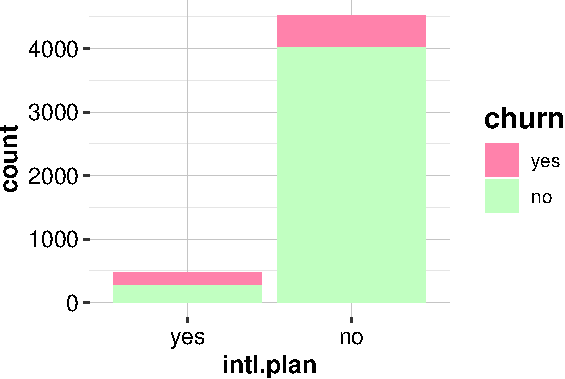
\includegraphics[width=0.5\linewidth,height=\textheight,keepaspectratio]{4-Exploratory-data-analysis_files/figure-pdf/unnamed-chunk-6-1.pdf}
\end{center}

The bar plot reveals a clear class imbalance: the majority of customers
remain active (\texttt{churn\ =\ "no"}), while a smaller proportion have
left the service (\texttt{churn\ =\ "yes"}). Approximately 14.1\% of
customers have churned.

This visualization builds on foundational plotting techniques introduced
in Section \ref{sec-ch1-visualization}. A simpler version, omitting
color and percentage labels, can be generated with:

\begin{Shaded}
\begin{Highlighting}[]
\FunctionTok{ggplot}\NormalTok{(}\AttributeTok{data =}\NormalTok{ churn) }\SpecialCharTok{+} 
  \FunctionTok{geom\_bar}\NormalTok{(}\FunctionTok{aes}\NormalTok{(}\AttributeTok{x =}\NormalTok{ churn))}
\end{Highlighting}
\end{Shaded}

While quick to produce, the simplified plot may be less informative in
presentation settings. Enhancements such as color coding and annotated
percentages improve clarity and are especially helpful when
communicating results to stakeholders without a technical background.

Class imbalance is more than a descriptive statistic; it can distort
predictive modeling by encouraging algorithms to favor the majority
class. We will return to this issue in Chapter \ref{sec-ch6-setup-data},
Section \ref{sec-ch6-balancing}, where methods for addressing imbalance
are introduced.

With this context in place, consider the next question: Are some service
features more closely associated with churn than others? To explore
this, we begin with the international calling plan.

\subsection*{Relationship Between Subscription Plans and
Churn}\label{relationship-between-subscription-plans-and-churn}
\addcontentsline{toc}{subsection}{Relationship Between Subscription
Plans and Churn}

Among the features available in the \emph{churn} dataset, the variable
\texttt{intl.plan} is especially relevant from a business and customer
experience standpoint. It indicates whether a customer subscribes to an
international calling plan, an option that may reflect unique
communication needs and cost sensitivities.

As a binary categorical variable, \texttt{intl.plan} allows for a
straightforward comparison of churn behavior between customers who do
and do not use international services.

\begin{Shaded}
\begin{Highlighting}[]
\FunctionTok{ggplot}\NormalTok{(}\AttributeTok{data =}\NormalTok{ churn) }\SpecialCharTok{+} 
  \FunctionTok{geom\_bar}\NormalTok{(}\FunctionTok{aes}\NormalTok{(}\AttributeTok{x =}\NormalTok{ intl.plan, }\AttributeTok{fill =}\NormalTok{ churn))    }

\FunctionTok{ggplot}\NormalTok{(}\AttributeTok{data =}\NormalTok{ churn) }\SpecialCharTok{+} 
  \FunctionTok{geom\_bar}\NormalTok{(}\FunctionTok{aes}\NormalTok{(}\AttributeTok{x =}\NormalTok{ intl.plan, }\AttributeTok{fill =}\NormalTok{ churn), }\AttributeTok{position =} \StringTok{"fill"}\NormalTok{) }
\end{Highlighting}
\end{Shaded}

\begin{figure}

\begin{minipage}{0.50\linewidth}
\begin{center}
\pandocbounded{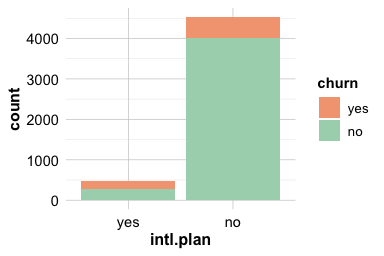
\includegraphics[keepaspectratio]{4-Exploratory-data-analysis_files/figure-pdf/unnamed-chunk-7-1.pdf}}
\end{center}
\end{minipage}%
%
\begin{minipage}{0.50\linewidth}
\begin{center}
\pandocbounded{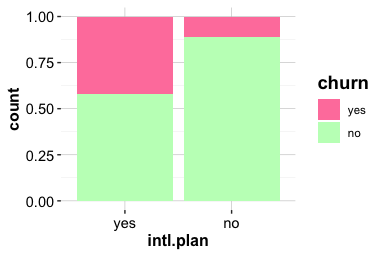
\includegraphics[keepaspectratio]{4-Exploratory-data-analysis_files/figure-pdf/unnamed-chunk-7-2.pdf}}
\end{center}
\end{minipage}%

\end{figure}%

The first plot shows the absolute number of churners and non-churners in
each group. The second, normalized by group size, reveals a sharper
insight: customers subscribed to an international plan are
disproportionately more likely to churn.

This observation can be formally examined using a contingency table:

\begin{Shaded}
\begin{Highlighting}[]
\FunctionTok{addmargins}\NormalTok{(}\FunctionTok{table}\NormalTok{(churn}\SpecialCharTok{$}\NormalTok{churn, churn}\SpecialCharTok{$}\NormalTok{intl.plan, }
                 \AttributeTok{dnn =} \FunctionTok{c}\NormalTok{(}\StringTok{"Churn"}\NormalTok{, }\StringTok{"International Plan"}\NormalTok{)))}
\NormalTok{        International Plan}
\NormalTok{   Churn  yes   no  Sum}
\NormalTok{     yes  }\DecValTok{199}  \DecValTok{508}  \DecValTok{707}
\NormalTok{     no   }\DecValTok{274} \DecValTok{4019} \DecValTok{4293}
\NormalTok{     Sum  }\DecValTok{473} \DecValTok{4527} \DecValTok{5000}
\end{Highlighting}
\end{Shaded}

The table confirms the visual pattern. Among those with an international
plan, the rate of churn is noticeably elevated. This may signal customer
dissatisfaction, possibly with pricing, call quality, or perceived
value.

Such findings have practical implications. Identifying segments with
elevated churn risk supports more informed retention strategies. For
example, international plan users might benefit from targeted offers,
feedback surveys, or enhanced service guarantees.

In the next subsection, we examine whether voice mail subscription shows
a similar or contrasting association with churn behavior.

\subsection*{Relationship Between Voice Mail Plan and
Churn}\label{relationship-between-voice-mail-plan-and-churn}
\addcontentsline{toc}{subsection}{Relationship Between Voice Mail Plan
and Churn}

We now turn to another service-related feature: the voice mail plan. The
variable \texttt{voice.plan} indicates whether a customer subscribes to
this additional feature. Like the international plan, it may reflect
aspects of customer engagement, satisfaction, or perceived value.

\begin{Shaded}
\begin{Highlighting}[]
\FunctionTok{ggplot}\NormalTok{(}\AttributeTok{data =}\NormalTok{ churn) }\SpecialCharTok{+} 
  \FunctionTok{geom\_bar}\NormalTok{(}\FunctionTok{aes}\NormalTok{(}\AttributeTok{x =}\NormalTok{ voice.plan, }\AttributeTok{fill =}\NormalTok{ churn))}

\FunctionTok{ggplot}\NormalTok{(}\AttributeTok{data =}\NormalTok{ churn) }\SpecialCharTok{+} 
  \FunctionTok{geom\_bar}\NormalTok{(}\FunctionTok{aes}\NormalTok{(}\AttributeTok{x =}\NormalTok{ voice.plan, }\AttributeTok{fill =}\NormalTok{ churn), }\AttributeTok{position =} \StringTok{"fill"}\NormalTok{) }
\end{Highlighting}
\end{Shaded}

\begin{figure}

\begin{minipage}{0.50\linewidth}
\begin{center}
\pandocbounded{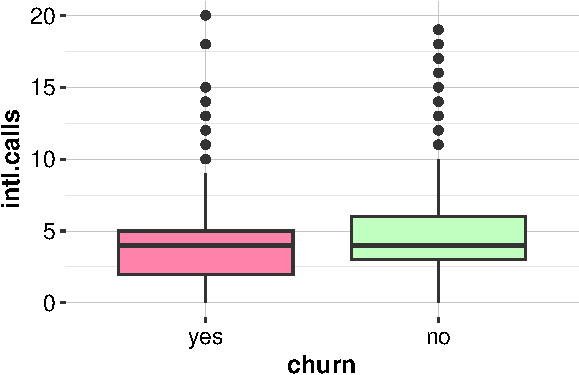
\includegraphics[keepaspectratio]{4-Exploratory-data-analysis_files/figure-pdf/unnamed-chunk-9-1.pdf}}
\end{center}
\end{minipage}%
%
\begin{minipage}{0.50\linewidth}
\begin{center}
\pandocbounded{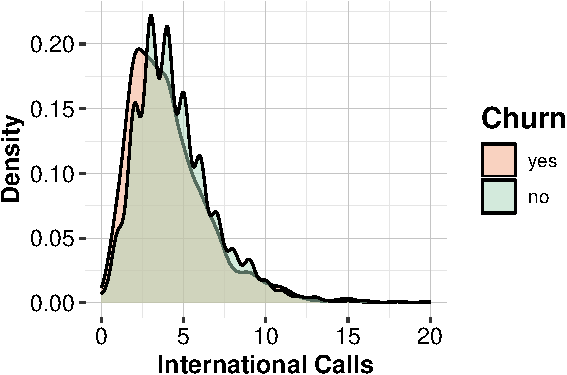
\includegraphics[keepaspectratio]{4-Exploratory-data-analysis_files/figure-pdf/unnamed-chunk-9-2.pdf}}
\end{center}
\end{minipage}%

\end{figure}%

The left panel displays the absolute number of customers who churned or
remained, segmented by voice mail plan subscription. The right panel
presents the same information in proportional form, highlighting
differences in churn rates between groups. While the difference is not
dramatic, customers with a voice mail plan appear to churn at slightly
lower rates.

To support this visual impression, we generate a contingency table:

\begin{Shaded}
\begin{Highlighting}[]
\FunctionTok{addmargins}\NormalTok{(}\FunctionTok{table}\NormalTok{(churn}\SpecialCharTok{$}\NormalTok{churn, churn}\SpecialCharTok{$}\NormalTok{voice.plan, }\AttributeTok{dnn =} \FunctionTok{c}\NormalTok{(}\StringTok{"Churn"}\NormalTok{, }\StringTok{"Voice Mail Plan"}\NormalTok{)))}
\NormalTok{        Voice Mail Plan}
\NormalTok{   Churn  yes   no  Sum}
\NormalTok{     yes  }\DecValTok{102}  \DecValTok{605}  \DecValTok{707}
\NormalTok{     no  }\DecValTok{1221} \DecValTok{3072} \DecValTok{4293}
\NormalTok{     Sum }\DecValTok{1323} \DecValTok{3677} \DecValTok{5000}
\end{Highlighting}
\end{Shaded}

The results confirm a modest association between voice mail usage and
customer retention. While less striking than the pattern observed for
the international calling plan, the trend may suggest that customers who
subscribe to add-on services are more engaged, or perhaps more satisfied
with their experience.

Even subtle effects can be meaningful in practice. In industries where
churn reduction drives profitability, small gains in retention can yield
significant impact. These early observations offer a foundation for
later predictive modeling and underscore the value of analyzing
categorical features in detail.

\subsection*{Summary of Categorical
Findings}\label{summary-of-categorical-findings}
\addcontentsline{toc}{subsection}{Summary of Categorical Findings}

The exploratory analysis of categorical variables reveals several early
signals that help frame the churn problem:

\begin{itemize}
\item
  Customers subscribed to an international calling plan are noticeably
  more likely to churn. This group may warrant closer attention, as it
  could reflect unmet service expectations or dissatisfaction with
  pricing.
\item
  Those who subscribe to a voice mail plan tend to churn less
  frequently, hinting at a possible link between service engagement and
  customer loyalty.
\item
  Even modest differences in churn rates across service features can
  help identify vulnerable segments and guide retention efforts.
\end{itemize}

These findings offer more than surface-level description; they begin to
connect customer characteristics to behavioral outcomes. As we move on
to numerical variables, we continue this investigative process, looking
for patterns that deepen our understanding of churn dynamics.

\section{Exploring Numerical Features}\label{sec-EDA-sec-numeric}

Now that we have examined categorical predictors, we shift our focus to
numerical features, variables that often capture the subtleties of
customer behavior. In the \emph{churn} dataset, these include patterns
of service usage and support interactions that may not be obvious at
first glance. While summary statistics provide a high-level overview, it
is through visual tools (e.g.~histograms, box plots, and density plots)
that meaningful trends, outliers, and predictive signals begin to
emerge. By visualizing these variables, we can uncover behavioral
patterns that may help explain why some customers stay and others leave.

\subsection*{Customer Service Calls and
Churn}\label{customer-service-calls-and-churn}
\addcontentsline{toc}{subsection}{Customer Service Calls and Churn}

What can frequent support calls tell us about customer satisfaction? The
variable \texttt{customer.calls} records how often each customer has
contacted customer service, a potentially revealing signal. High contact
frequency may indicate dissatisfaction, unresolved problems, or greater
service dependency, all of which can raise the risk of churn.

We begin by visualizing the distribution of this variable:

\begin{Shaded}
\begin{Highlighting}[]
\FunctionTok{ggplot}\NormalTok{(}\AttributeTok{data =}\NormalTok{ churn) }\SpecialCharTok{+}
  \FunctionTok{geom\_bar}\NormalTok{(}\FunctionTok{aes}\NormalTok{(}\AttributeTok{x =} \FunctionTok{factor}\NormalTok{(customer.calls)), }\AttributeTok{fill =} \StringTok{"\#80CDC1"}\NormalTok{, }\AttributeTok{color =} \StringTok{"black"}\NormalTok{) }\SpecialCharTok{+}
  \FunctionTok{labs}\NormalTok{(}\AttributeTok{x =} \StringTok{"Number of Service Calls"}\NormalTok{, }\AttributeTok{y =} \StringTok{"Count"}\NormalTok{)}
\end{Highlighting}
\end{Shaded}

\begin{center}
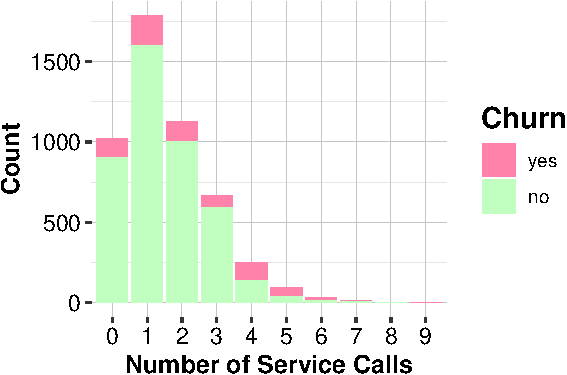
\includegraphics[width=0.6\linewidth,height=\textheight,keepaspectratio]{4-Exploratory-data-analysis_files/figure-pdf/unnamed-chunk-11-1.pdf}
\end{center}

Because \texttt{customer.calls} is a count variable with a small number
of discrete values (ranging from 0 to 9), we convert it to a factor and
use a bar plot to highlight its distribution. While a histogram could be
used, it offers little advantage here due to the limited number of
distinct values. In contrast, density plots or box plots are less
suitable and may obscure meaningful patterns.

The bar plot reveals a right-skewed distribution: most customers contact
support rarely, while a smaller group makes frequent calls. To explore
how this behavior relates to churn, we compare service call frequency
across churn outcomes:

\begin{Shaded}
\begin{Highlighting}[]
\FunctionTok{ggplot}\NormalTok{(}\AttributeTok{data =}\NormalTok{ churn) }\SpecialCharTok{+}
  \FunctionTok{geom\_bar}\NormalTok{(}\FunctionTok{aes}\NormalTok{(}\AttributeTok{x =} \FunctionTok{factor}\NormalTok{(customer.calls), }\AttributeTok{fill =}\NormalTok{ churn), }\AttributeTok{position =} \StringTok{"stack"}\NormalTok{) }\SpecialCharTok{+}
  \FunctionTok{labs}\NormalTok{(}\AttributeTok{x =} \StringTok{"Number of Service Calls"}\NormalTok{, }\AttributeTok{y =} \StringTok{"Count"}\NormalTok{, }\AttributeTok{fill =} \StringTok{"Churn"}\NormalTok{) }

\FunctionTok{ggplot}\NormalTok{(}\AttributeTok{data =}\NormalTok{ churn) }\SpecialCharTok{+}
  \FunctionTok{geom\_bar}\NormalTok{(}\FunctionTok{aes}\NormalTok{(}\AttributeTok{x =} \FunctionTok{factor}\NormalTok{(customer.calls), }\AttributeTok{fill =}\NormalTok{ churn), }\AttributeTok{position =} \StringTok{"fill"}\NormalTok{) }\SpecialCharTok{+}
  \FunctionTok{labs}\NormalTok{(}\AttributeTok{x =} \StringTok{"Number of Service Calls"}\NormalTok{, }\AttributeTok{y =} \StringTok{"Proportion"}\NormalTok{, }\AttributeTok{fill =} \StringTok{"Churn"}\NormalTok{) }
\end{Highlighting}
\end{Shaded}

\begin{figure}

\begin{minipage}{0.50\linewidth}
\begin{center}
\pandocbounded{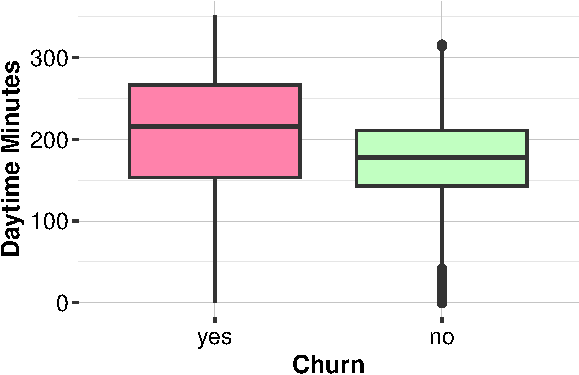
\includegraphics[keepaspectratio]{4-Exploratory-data-analysis_files/figure-pdf/unnamed-chunk-12-1.pdf}}
\end{center}
\end{minipage}%
%
\begin{minipage}{0.50\linewidth}
\begin{center}
\pandocbounded{\includegraphics[keepaspectratio]{4-Exploratory-data-analysis_files/figure-pdf/unnamed-chunk-12-2.pdf}}
\end{center}
\end{minipage}%

\end{figure}%

The left plot shows raw counts of churners and non-churners at each call
level. The right plot, normalized by call frequency, reveals a clear
trend: customers who make \emph{four or more service calls} are
significantly more likely to churn.

This pattern suggests that frequent contact with customer service may
signal dissatisfaction or unmet expectations. From a business
perspective, this insight could inform retention strategies, for
example, flagging at-risk customers after their third support call. From
a modeling perspective, creating a binary feature such as ``frequent
caller'' may better capture this non-linear trend than using the raw
count alone.

These kinds of behavioral signals are precisely what EDA is designed to
uncover. In the next subsection, we shift our focus to usage patterns,
starting with daytime call minutes.

\subsection*{Daytime Minutes and Churn}\label{daytime-minutes-and-churn}
\addcontentsline{toc}{subsection}{Daytime Minutes and Churn}

Do customers who use their phone service more frequently during the day
also churn more often? One variable that can help answer this is
\texttt{day.mins}, which records the number of minutes each customer
spends on daytime calls. High daytime usage may indicate stronger
dependency on the service, along with heightened sensitivity to pricing,
call quality, or reliability.

Because \texttt{day.mins} is a continuous numerical variable, we use a
box plot to compare distributions across churn outcomes and a density
plot to visualize the shape of each distribution. These plots help
detect shifts, spread, and overlap between groups. You could also
explore this variable with a histogram, which offers another view of
distribution---try generating one using \texttt{geom\_histogram()} as an
exercise.

\begin{Shaded}
\begin{Highlighting}[]
\FunctionTok{ggplot}\NormalTok{(}\AttributeTok{data =}\NormalTok{ churn) }\SpecialCharTok{+}
  \FunctionTok{geom\_boxplot}\NormalTok{(}\FunctionTok{aes}\NormalTok{(}\AttributeTok{x =}\NormalTok{ churn, }\AttributeTok{y =}\NormalTok{ day.mins), }
               \AttributeTok{fill =} \FunctionTok{c}\NormalTok{(}\StringTok{"\#F4A582"}\NormalTok{, }\StringTok{"\#A8D5BA"}\NormalTok{)) }\SpecialCharTok{+}
  \FunctionTok{labs}\NormalTok{(}\AttributeTok{x =} \StringTok{"Churn"}\NormalTok{, }\AttributeTok{y =} \StringTok{"Daytime Minutes"}\NormalTok{)}

\FunctionTok{ggplot}\NormalTok{(}\AttributeTok{data =}\NormalTok{ churn) }\SpecialCharTok{+}
  \FunctionTok{geom\_density}\NormalTok{(}\FunctionTok{aes}\NormalTok{(}\AttributeTok{x =}\NormalTok{ day.mins, }\AttributeTok{fill =}\NormalTok{ churn), }\AttributeTok{alpha =} \FloatTok{0.5}\NormalTok{) }\SpecialCharTok{+}
  \FunctionTok{labs}\NormalTok{(}\AttributeTok{x =} \StringTok{"Daytime Minutes"}\NormalTok{, }\AttributeTok{y =} \StringTok{"Density"}\NormalTok{, }\AttributeTok{fill =} \StringTok{"Churn"}\NormalTok{)}
\end{Highlighting}
\end{Shaded}

\begin{figure}

\begin{minipage}{0.50\linewidth}
\begin{center}
\pandocbounded{\includegraphics[keepaspectratio]{4-Exploratory-data-analysis_files/figure-pdf/unnamed-chunk-13-1.pdf}}
\end{center}
\end{minipage}%
%
\begin{minipage}{0.50\linewidth}
\begin{center}
\pandocbounded{\includegraphics[keepaspectratio]{4-Exploratory-data-analysis_files/figure-pdf/unnamed-chunk-13-2.pdf}}
\end{center}
\end{minipage}%

\end{figure}%

The box plot shows that customers who churn tend to have higher daytime
usage, and the density plot confirms this shift. While the difference is
not dramatic, it is consistent, suggesting that high-usage customers may
be at elevated churn risk.

\emph{Key Insights and Business Implications}: Customers with high
\texttt{day.mins} usage are more likely to churn. This trend may reflect
dissatisfaction driven by unmet service expectations or cost concerns.
From a business perspective, proactive retention strategies, such as
personalized plans or loyalty benefits, could help retain high-usage
customers. From a modeling perspective, \texttt{day.mins} is a valuable
predictor and may also interact with other features such as
\texttt{day.charge} or \texttt{customer.calls}.

\subsection*{Evening and Nighttime
Minutes}\label{evening-and-nighttime-minutes}
\addcontentsline{toc}{subsection}{Evening and Nighttime Minutes}

Do customers who make more evening or nighttime calls tend to churn more
often? To investigate this, we examine two numerical features:
\texttt{eve.mins}, which measures total minutes of evening calls, and
\texttt{night.mins}, which records nighttime usage. These time periods
may reflect different customer routines, pricing structures, or service
expectations compared to daytime activity.

Since both variables are continuous, we begin by visualizing
\texttt{eve.mins} using a violin plot layered with a box plot to show
distributional shape and spread, and a density plot to examine the
overlap between churners and non-churners:

\begin{Shaded}
\begin{Highlighting}[]
\FunctionTok{ggplot}\NormalTok{(}\AttributeTok{data =}\NormalTok{ churn, }\FunctionTok{aes}\NormalTok{(}\AttributeTok{x =}\NormalTok{ churn, }\AttributeTok{y =}\NormalTok{ eve.mins)) }\SpecialCharTok{+}
  \FunctionTok{geom\_violin}\NormalTok{(}\AttributeTok{trim =} \ConstantTok{FALSE}\NormalTok{) }\SpecialCharTok{+} 
  \FunctionTok{geom\_boxplot}\NormalTok{(}\AttributeTok{width =} \FloatTok{0.3}\NormalTok{, }\AttributeTok{fill =} \FunctionTok{c}\NormalTok{(}\StringTok{"\#F4A582"}\NormalTok{, }\StringTok{"\#A8D5BA"}\NormalTok{)) }\SpecialCharTok{+}
  \FunctionTok{labs}\NormalTok{(}\AttributeTok{x =} \StringTok{"Churn"}\NormalTok{, }\AttributeTok{y =} \StringTok{"Evening Minutes"}\NormalTok{)}

\FunctionTok{ggplot}\NormalTok{(}\AttributeTok{data =}\NormalTok{ churn) }\SpecialCharTok{+}
  \FunctionTok{geom\_density}\NormalTok{(}\FunctionTok{aes}\NormalTok{(}\AttributeTok{x =}\NormalTok{ eve.mins, }\AttributeTok{fill =}\NormalTok{ churn), }\AttributeTok{alpha =} \FloatTok{0.5}\NormalTok{) }\SpecialCharTok{+}
  \FunctionTok{labs}\NormalTok{(}\AttributeTok{x =} \StringTok{"Evening Minutes"}\NormalTok{, }\AttributeTok{y =} \StringTok{"Density"}\NormalTok{, }\AttributeTok{fill =} \StringTok{"Churn"}\NormalTok{)}
\end{Highlighting}
\end{Shaded}

\begin{figure}

\begin{minipage}{0.50\linewidth}
\begin{center}
\pandocbounded{\includegraphics[keepaspectratio]{4-Exploratory-data-analysis_files/figure-pdf/unnamed-chunk-14-1.pdf}}
\end{center}
\end{minipage}%
%
\begin{minipage}{0.50\linewidth}
\begin{center}
\pandocbounded{\includegraphics[keepaspectratio]{4-Exploratory-data-analysis_files/figure-pdf/unnamed-chunk-14-2.pdf}}
\end{center}
\end{minipage}%

\end{figure}%

The visualizations suggest a slight shift toward higher evening call
usage among churners, but the overlap between groups remains
substantial. Compared to \texttt{day.mins}, the association here is
clearly weaker.

We now apply the same approach to \texttt{night.mins}:

\begin{Shaded}
\begin{Highlighting}[]
\FunctionTok{ggplot}\NormalTok{(}\AttributeTok{data =}\NormalTok{ churn) }\SpecialCharTok{+}
  \FunctionTok{geom\_boxplot}\NormalTok{(}\FunctionTok{aes}\NormalTok{(}\AttributeTok{x =}\NormalTok{ churn, }\AttributeTok{y =}\NormalTok{ night.mins), }\AttributeTok{fill =} \FunctionTok{c}\NormalTok{(}\StringTok{"\#F4A582"}\NormalTok{, }\StringTok{"\#A8D5BA"}\NormalTok{)) }\SpecialCharTok{+}
  \FunctionTok{labs}\NormalTok{(}\AttributeTok{x =} \StringTok{"Churn"}\NormalTok{, }\AttributeTok{y =} \StringTok{"Nighttime Minutes"}\NormalTok{)}

\FunctionTok{ggplot}\NormalTok{(}\AttributeTok{data =}\NormalTok{ churn) }\SpecialCharTok{+}
  \FunctionTok{geom\_density}\NormalTok{(}\FunctionTok{aes}\NormalTok{(}\AttributeTok{x =}\NormalTok{ night.mins, }\AttributeTok{fill =}\NormalTok{ churn), }\AttributeTok{alpha =} \FloatTok{0.5}\NormalTok{) }\SpecialCharTok{+}
  \FunctionTok{labs}\NormalTok{(}\AttributeTok{x =} \StringTok{"Nighttime Minutes"}\NormalTok{, }\AttributeTok{y =} \StringTok{"Density"}\NormalTok{, }\AttributeTok{fill =} \StringTok{"Churn"}\NormalTok{)}
\end{Highlighting}
\end{Shaded}

\begin{figure}

\begin{minipage}{0.50\linewidth}
\begin{center}
\pandocbounded{\includegraphics[keepaspectratio]{4-Exploratory-data-analysis_files/figure-pdf/unnamed-chunk-15-1.pdf}}
\end{center}
\end{minipage}%
%
\begin{minipage}{0.50\linewidth}
\begin{center}
\pandocbounded{\includegraphics[keepaspectratio]{4-Exploratory-data-analysis_files/figure-pdf/unnamed-chunk-15-2.pdf}}
\end{center}
\end{minipage}%

\end{figure}%

The box and density plots for nighttime usage reveal no meaningful
difference between churners and non-churners, suggesting little
association with churn behavior.

\emph{Key Insights and Business Implications}: Evening and nighttime
usage show limited individual predictive power. While \texttt{eve.mins}
may be slightly elevated for churners, the effect is modest and
inconsistent. These variables are unlikely to drive churn predictions on
their own but may contribute in combination with other features. For
practical applications, they are best interpreted as part of a broader
usage pattern rather than in isolation.

\subsection*{International Calls and
Churn}\label{international-calls-and-churn}
\addcontentsline{toc}{subsection}{International Calls and Churn}

In a previous section, we observed that customers subscribed to an
international calling plan are more likely to churn. But does actual
calling behavior support this pattern? The variable \texttt{intl.calls}
records the total number of international calls placed by each customer,
providing a behavioral counterpart to the plan subscription flag.

Because \texttt{intl.calls} is a discrete numeric variable with moderate
range, we examine its distribution by churn status using a box plot and
a density plot:

\begin{Shaded}
\begin{Highlighting}[]
\FunctionTok{ggplot}\NormalTok{(}\AttributeTok{data =}\NormalTok{ churn) }\SpecialCharTok{+}
  \FunctionTok{geom\_boxplot}\NormalTok{(}\FunctionTok{aes}\NormalTok{(}\AttributeTok{x =}\NormalTok{ churn, }\AttributeTok{y =}\NormalTok{ intl.calls), }
               \AttributeTok{fill =} \FunctionTok{c}\NormalTok{(}\StringTok{"\#F4A582"}\NormalTok{, }\StringTok{"\#A8D5BA"}\NormalTok{)) }\SpecialCharTok{+}
  \FunctionTok{labs}\NormalTok{(}\AttributeTok{x =} \StringTok{"Churn"}\NormalTok{, }\AttributeTok{y =} \StringTok{"International Calls"}\NormalTok{)}

\FunctionTok{ggplot}\NormalTok{(}\AttributeTok{data =}\NormalTok{ churn) }\SpecialCharTok{+}
  \FunctionTok{geom\_density}\NormalTok{(}\FunctionTok{aes}\NormalTok{(}\AttributeTok{x =}\NormalTok{ intl.calls, }\AttributeTok{fill =}\NormalTok{ churn), }\AttributeTok{alpha =} \FloatTok{0.5}\NormalTok{) }\SpecialCharTok{+}
  \FunctionTok{labs}\NormalTok{(}\AttributeTok{x =} \StringTok{"International Calls"}\NormalTok{, }\AttributeTok{y =} \StringTok{"Density"}\NormalTok{, }\AttributeTok{fill =} \StringTok{"Churn"}\NormalTok{)}
\end{Highlighting}
\end{Shaded}

\begin{figure}

\begin{minipage}{0.50\linewidth}
\begin{center}
\pandocbounded{\includegraphics[keepaspectratio]{4-Exploratory-data-analysis_files/figure-pdf/unnamed-chunk-16-1.pdf}}
\end{center}
\end{minipage}%
%
\begin{minipage}{0.50\linewidth}
\begin{center}
\pandocbounded{\includegraphics[keepaspectratio]{4-Exploratory-data-analysis_files/figure-pdf/unnamed-chunk-16-2.pdf}}
\end{center}
\end{minipage}%

\end{figure}%

The visualizations suggest that churners make slightly fewer
international calls than non-churners. However, the difference is small
and the distributions overlap considerably.

\emph{Key Insights and Business Implications}: The \texttt{intl.calls}
variable shows only a weak association with churn. This finding suggests
that subscribing to an international plan (a binary indicator) may
matter more than how much it is actually used. Formal statistical
testing, such as a two-sample t-test, can help assess whether the
observed difference is significant. We will revisit this question in
Chapter \ref{sec-ch5-statistics} when discussing hypothesis testing.

\subsection*{Summary of Numerical
Findings}\label{summary-of-numerical-findings}
\addcontentsline{toc}{subsection}{Summary of Numerical Findings}

The exploratory analysis of numerical features in the \emph{churn}
dataset reveals the following key patterns:

\begin{itemize}
\item
  \texttt{customer.calls} and \texttt{day.mins} are most strongly
  associated with churn. Customers making four or more service calls,
  and those with high daytime call usage, are more likely to leave the
  service.
\item
  These features are likely to play an important role in predictive
  modeling and may serve as effective early indicators for targeted
  retention strategies.
\item
  Other variables, such as \texttt{eve.mins}, \texttt{night.mins}, and
  \texttt{intl.calls}, show weaker or inconsistent associations with
  churn when analyzed individually. Their value may become clearer in
  multivariate contexts or when interacting with other predictors.
\end{itemize}

These findings will inform both feature selection and model development
in later chapters. In the next section, we examine relationships between
variables to detect potential redundancy and explore more complex
patterns relevant to classification tasks.

\section{Identifying Redundancy and Correlated
Features}\label{sec-ch4-EDA-correlation}

Before analyzing more complex interactions among variables, it is
helpful to assess how individual features relate to one another.
Correlation analysis is a key tool in this process, revealing variables
that may carry overlapping information or exhibit redundancy.
Identifying such relationships early not only simplifies the modeling
process but also enhances interpretability and reduces the risk of
multicollinearity.

Correlation quantifies the degree to which two variables move together.
A positive correlation indicates that as one variable increases, the
other tends to increase as well; a negative correlation suggests that
one tends to decrease as the other increases. If there is little or no
correlation, changes in one variable do not help predict changes in the
other. This relationship is typically summarized using the Pearson
correlation coefficient, denoted by \(r\), which ranges from \(-1\) to
\(1\). A value of \(r = 1\) implies a perfect positive linear
relationship, \(r = -1\) implies a perfect negative one, and \(r = 0\)
suggests no linear association.

Figure~\ref{fig-correlation} illustrates scatterplots with various
degrees of correlation.

\begin{figure}[H]

\centering{

\includegraphics[width=1\linewidth,height=\textheight,keepaspectratio]{images/ch4_correlation.png}

}

\caption{\label{fig-correlation}Example scatterplots showing different
correlation coefficients.}

\end{figure}%

\begin{quote}
\emph{Note:} Correlation does not imply causation. For example, a strong
positive correlation between customer service calls and churn does not
mean that making service calls \emph{causes} customers to leave. Rather,
both behaviors may stem from an underlying factor, such as
dissatisfaction with service.
\end{quote}

To underscore this caution, Figure \ref{fig-correlation-chocolate}
presents a memorable example from Messerli (2012). It shows a
surprisingly strong correlation between per-capita chocolate consumption
and Nobel Prize wins across countries. While entertaining, the example
highlights a key message: correlations may arise from coincidence,
reverse causality, or the influence of a third variable. For readers
interested in exploring causality and causal inference further,
\emph{The Book of Why} by Judea Pearl and Dana Mackenzie (Pearl and
Mackenzie 2018) offers an accessible treatment of the subject from both
statistical and philosophical perspectives.

\begin{figure}[H]

\centering{

\includegraphics[width=0.7\linewidth,height=\textheight,keepaspectratio]{images/ch4_correlation_chocolate.png}

}

\caption{\label{fig-correlation-chocolate}Scatterplot illustrating the
correlation between Nobel Prize wins and chocolate consumption (per 10
million population) across countries. Adapted from Messerli (2012).}

\end{figure}%

Returning to our dataset, we now compute and visualize the correlation
matrix for key numerical variables using a heatmap. This is done using
the \texttt{ggcorrplot()} function from the \textbf{ggcorrplot} package,
an extension of \textbf{ggplot2} that produces clean, annotated
correlation plots. It allows users to customize triangle display, label
coefficients, and control aesthetics for better interpretation.

\begin{Shaded}
\begin{Highlighting}[]
\FunctionTok{library}\NormalTok{(ggcorrplot)}

\NormalTok{variable\_list }\OtherTok{=} \FunctionTok{c}\NormalTok{(}\StringTok{"intl.mins"}\NormalTok{,  }\StringTok{"intl.calls"}\NormalTok{,  }\StringTok{"intl.charge"}\NormalTok{, }
                  \StringTok{"day.mins"}\NormalTok{,   }\StringTok{"day.calls"}\NormalTok{,   }\StringTok{"day.charge"}\NormalTok{,}
                  \StringTok{"eve.mins"}\NormalTok{,   }\StringTok{"eve.calls"}\NormalTok{,   }\StringTok{"eve.charge"}\NormalTok{,}
                  \StringTok{"night.mins"}\NormalTok{, }\StringTok{"night.calls"}\NormalTok{, }\StringTok{"night.charge"}\NormalTok{)}

\NormalTok{cor\_matrix }\OtherTok{=} \FunctionTok{cor}\NormalTok{(churn[, variable\_list])}

\FunctionTok{ggcorrplot}\NormalTok{(cor\_matrix, }\AttributeTok{type =} \StringTok{"upper"}\NormalTok{, }\AttributeTok{lab =} \ConstantTok{TRUE}\NormalTok{, }\AttributeTok{lab\_size =} \DecValTok{2}\NormalTok{, }\AttributeTok{tl.cex =} \DecValTok{8}\NormalTok{, }
           \AttributeTok{colors =} \FunctionTok{c}\NormalTok{(}\StringTok{"\#6D9EC1"}\NormalTok{, }\StringTok{"white"}\NormalTok{, }\StringTok{"\#E46726"}\NormalTok{),}
           \AttributeTok{title =} \StringTok{"Visualization of the Correlation Matrix"}\NormalTok{)}
\end{Highlighting}
\end{Shaded}

\begin{center}
\includegraphics[width=1\linewidth,height=\textheight,keepaspectratio]{4-Exploratory-data-analysis_files/figure-pdf/unnamed-chunk-17-1.pdf}
\end{center}

The resulting heatmap highlights two main patterns. First, the
\emph{charge variables} (such as \texttt{day.charge},
\texttt{eve.charge}, and \texttt{intl.charge}) are perfectly correlated
with their corresponding \emph{minutes variables}. This is expected, as
charges are calculated directly from call duration. Including both in a
model would add redundancy without new information.

Second, the \emph{call count variables} (e.g., \texttt{day.calls},
\texttt{night.calls}) show only weak correlations with their
corresponding \emph{minutes variables}. This suggests that call
frequency and call duration capture distinct aspects of user behavior
and should be considered complementary rather than interchangeable.

Based on these findings, it is advisable to remove the charge variables
when preparing the dataset for modeling, while retaining both frequency
and duration measures. Doing so streamlines the feature set, avoids
multicollinearity, and contributes to more interpretable and stable
predictive models.

\section{Exploring Multivariate
Relationships}\label{sec-EDA-sec-multivariate}

While correlation analysis helps identify linear associations between
pairs of variables, it often misses important patterns that emerge only
when multiple features are considered together. Multivariate analysis
enables us to explore such interactions and conditional relationships,
insights that are crucial for understanding complex behaviors like
customer churn.

Let us begin by jointly analyzing \texttt{day.mins} (daytime call
duration) and \texttt{eve.mins} (evening call duration). Are customers
who use the service heavily during both periods more likely to leave?

\begin{Shaded}
\begin{Highlighting}[]
\FunctionTok{ggplot}\NormalTok{(}\AttributeTok{data =}\NormalTok{ churn) }\SpecialCharTok{+}
    \FunctionTok{geom\_point}\NormalTok{(}\FunctionTok{aes}\NormalTok{(}\AttributeTok{x =}\NormalTok{ eve.mins, }\AttributeTok{y =}\NormalTok{ day.mins, }\AttributeTok{color =}\NormalTok{ churn), }\AttributeTok{size =} \FloatTok{0.7}\NormalTok{) }\SpecialCharTok{+}
    \FunctionTok{geom\_abline}\NormalTok{(}\AttributeTok{intercept =} \DecValTok{400}\NormalTok{, }\AttributeTok{slope =} \SpecialCharTok{{-}}\FloatTok{0.6}\NormalTok{, }\AttributeTok{color =} \StringTok{"\#377EB8"}\NormalTok{, }\AttributeTok{linewidth =} \DecValTok{1}\NormalTok{) }\SpecialCharTok{+} 
    \FunctionTok{scale\_color\_manual}\NormalTok{(}\AttributeTok{values =} \FunctionTok{c}\NormalTok{(}\StringTok{"\#F4A582"}\NormalTok{, }\StringTok{"\#A8D5BA"}\NormalTok{)) }\SpecialCharTok{+} 
    \FunctionTok{labs}\NormalTok{(}\AttributeTok{x =} \StringTok{"Evening Minutes"}\NormalTok{, }\AttributeTok{y =} \StringTok{"Daytime Minutes"}\NormalTok{, }\AttributeTok{color =} \StringTok{"Churn"}\NormalTok{)}
\end{Highlighting}
\end{Shaded}

\begin{center}
\includegraphics[width=0.65\linewidth,height=\textheight,keepaspectratio]{4-Exploratory-data-analysis_files/figure-pdf/unnamed-chunk-18-1.pdf}
\end{center}

To help identify behavioral segments, we add a diagonal line using
\texttt{geom\_abline()}, which overlays a reference line with a given
intercept and slope. This line represents the boundary:

\[
\text{day.mins} = 400 - 0.6 \times \text{eve.mins}
\]

Customers above this line, those with \emph{simultaneously high day and
evening usage}, show a noticeably greater tendency to churn. This
insight would not be visible from analyzing either variable in
isolation, highlighting the importance of considering variable
interactions.

To quantify this finding, we isolate this high-usage group using the
\texttt{subset()} function:

\begin{Shaded}
\begin{Highlighting}[]
\NormalTok{sub\_churn }\OtherTok{=} \FunctionTok{subset}\NormalTok{(churn, (day.mins }\SpecialCharTok{\textgreater{}} \DecValTok{400} \SpecialCharTok{{-}} \FloatTok{0.6} \SpecialCharTok{*}\NormalTok{ eve.mins))}

\FunctionTok{ggplot}\NormalTok{(}\AttributeTok{data =}\NormalTok{ sub\_churn, }\FunctionTok{aes}\NormalTok{(}\AttributeTok{x =}\NormalTok{ churn, }\AttributeTok{label =}\NormalTok{ scales}\SpecialCharTok{::}\FunctionTok{percent}\NormalTok{(}\FunctionTok{prop.table}\NormalTok{(}\FunctionTok{stat}\NormalTok{(count))))) }\SpecialCharTok{+}
    \FunctionTok{geom\_bar}\NormalTok{(}\AttributeTok{fill =} \FunctionTok{c}\NormalTok{(}\StringTok{"\#F4A582"}\NormalTok{, }\StringTok{"\#A8D5BA"}\NormalTok{)) }\SpecialCharTok{+} 
    \FunctionTok{geom\_text}\NormalTok{(}\AttributeTok{stat =} \StringTok{\textquotesingle{}count\textquotesingle{}}\NormalTok{, }\AttributeTok{vjust =} \FloatTok{0.4}\NormalTok{, }\AttributeTok{size =} \DecValTok{8}\NormalTok{)}
\end{Highlighting}
\end{Shaded}

\begin{center}
\includegraphics[width=0.5\linewidth,height=\textheight,keepaspectratio]{4-Exploratory-data-analysis_files/figure-pdf/unnamed-chunk-19-1.pdf}
\end{center}

The churn rate within this group is approximately 71.5\%, compared to an
overall churn rate of 14.1\%. This difference suggests that intensive
usage across multiple periods may be a signal of dissatisfaction,
possibly related to billing complexity or service expectations.

Next, we examine another potential interaction: the relationship between
\texttt{customer.calls} and \texttt{day.mins}.

\begin{Shaded}
\begin{Highlighting}[]
\FunctionTok{ggplot}\NormalTok{(}\AttributeTok{data =}\NormalTok{ churn, }\FunctionTok{aes}\NormalTok{(}\AttributeTok{x =}\NormalTok{ day.mins, }\AttributeTok{y =}\NormalTok{ customer.calls, }\AttributeTok{color =}\NormalTok{ churn)) }\SpecialCharTok{+}
  \FunctionTok{geom\_point}\NormalTok{(}\AttributeTok{size =} \DecValTok{1}\NormalTok{) }\SpecialCharTok{+}
  \FunctionTok{geom\_point}\NormalTok{(}\AttributeTok{data =} \FunctionTok{data.frame}\NormalTok{(}\AttributeTok{day.mins =} \DecValTok{110}\NormalTok{, }\AttributeTok{customer.calls =} \FloatTok{5.5}\NormalTok{), }\AttributeTok{colour =} \StringTok{"\#377EB8"}\NormalTok{, }\AttributeTok{size =} \DecValTok{50}\NormalTok{, }\AttributeTok{shape =} \DecValTok{1}\NormalTok{) }\SpecialCharTok{+} 
  \FunctionTok{geom\_point}\NormalTok{(}\AttributeTok{data =} \FunctionTok{data.frame}\NormalTok{(}\AttributeTok{day.mins =} \DecValTok{310}\NormalTok{, }\AttributeTok{customer.calls =} \FloatTok{2.0}\NormalTok{), }\AttributeTok{colour =} \StringTok{"\#377EB8"}\NormalTok{, }\AttributeTok{size =} \DecValTok{40}\NormalTok{, }\AttributeTok{shape =} \DecValTok{1}\NormalTok{) }\SpecialCharTok{+}
  \FunctionTok{scale\_color\_manual}\NormalTok{(}\AttributeTok{values =} \FunctionTok{c}\NormalTok{(}\StringTok{"\#F4A582"}\NormalTok{, }\StringTok{"\#A8D5BA"}\NormalTok{)) }\SpecialCharTok{+}
  \FunctionTok{labs}\NormalTok{(}\AttributeTok{x =} \StringTok{"Daytime Minutes"}\NormalTok{, }\AttributeTok{y =} \StringTok{"Customer Service Calls"}\NormalTok{, }\AttributeTok{color =} \StringTok{"Churn"}\NormalTok{)}
\end{Highlighting}
\end{Shaded}

\begin{center}
\includegraphics[width=0.65\linewidth,height=\textheight,keepaspectratio]{4-Exploratory-data-analysis_files/figure-pdf/unnamed-chunk-20-1.pdf}
\end{center}

This scatter plot highlights an interesting pattern. Customers who
contact support frequently but have low usage (blue circle, top-left)
tend to churn at higher rates, perhaps reflecting frustration despite
limited use of the service. In contrast, customers with both high usage
and frequent support contact (blue circle, bottom-right) show more mixed
churn outcomes, possibly because they value the service highly even when
problems arise.

Together, these examples illustrate how multivariate analysis can expose
interaction effects and behavioral subgroups that are not apparent in
simpler analyses. From a modeling perspective, such findings suggest
opportunities to engineer features that capture joint effects, such as
interaction terms or binary flags for high-risk combinations. From a
business standpoint, these insights can guide proactive interventions
aimed at specific customer profiles.

In Chapter \ref{sec-ch5-statistics}, we return to these findings using
formal statistical methods to assess their significance and evaluate
their role in predictive modeling.

\section{Insights from EDA on Customer Churn}\label{sec-EDA-summary}

The exploratory analysis of the \emph{churn} dataset has revealed
several behavioral patterns and feature relationships that are relevant
to both modeling and business strategy. By systematically examining
individual variables and their interactions, we identified predictors of
customer attrition and gained a deeper understanding of usage and
support dynamics.

One of the most salient findings is the association between customer
service interactions and churn. Customers who contact support four or
more times are substantially more likely to leave the service, pointing
to dissatisfaction or unresolved problems. This pattern suggests a need
for early intervention based on support behavior.

High combined usage of daytime and evening minutes also emerged as a
strong churn signal. Customers in this segment exhibit churn rates
several times higher than the average, likely reflecting unmet
expectations related to pricing, billing, or service quality. Similarly,
frequent service calls paired with low daytime usage define another
at-risk segment, one that would not be evident in univariate summaries
alone.

The presence of an international calling plan is another key predictor:
customers subscribed to this plan churn at significantly higher rates.
In contrast, customers with a voice mail plan are less likely to churn,
suggesting that certain service features may promote retention.

The analysis also highlighted opportunities to streamline the feature
set. Charge variables, which are perfectly correlated with call
durations, should be removed to reduce redundancy and avoid
multicollinearity. In addition, variables such as \texttt{state} and
\texttt{area.code} appear to offer limited predictive value and may be
excluded from modeling unless interaction effects are hypothesized.

These insights inform several strategic directions. Customers making
their third support call could be flagged for proactive retention
efforts, such as tailored offers or escalated service handling.
High-usage customers may benefit from personalized rate plans or loyalty
incentives. The international plan should be reevaluated for its pricing
structure and value proposition. And voice mail features could be more
prominently marketed or bundled as part of retention strategies.

Even variables with weak individual associations, such as nighttime
minutes, may still contribute predictive value in combination with other
features. Their joint effects will be assessed in subsequent chapters
through statistical testing and machine learning.

By uncovering these behavioral patterns through exploratory analysis, we
have laid the groundwork for the next phase of the data science
workflow: building predictive models that quantify risk and support
decision-making. In the next chapter, we introduce statistical tools to
formalize the relationships observed here, setting the stage for
classification models such as logistic regression and k-nearest
neighbors.

\section{Chapter Summary and
Takeaways}\label{chapter-summary-and-takeaways-3}

This chapter introduced EDA as a foundational step in the data science
workflow, an approach that emphasizes curiosity-driven inquiry guided by
patterns within the data. Unlike confirmatory analysis, EDA does not
begin with fixed hypotheses; rather, it involves iterative examination
through descriptive statistics, visualizations, and correlation measures
to uncover structure, relationships, and irregularities.

Drawing on the \emph{churn} dataset, we investigated behavioral signals
associated with customer attrition. The analysis revealed that frequent
contact with customer service, heavy usage during both daytime and
evening hours, and enrollment in international calling plans were linked
to a heightened risk of churn. Conversely, customers subscribed to a
voice mail plan were more likely to stay, suggesting that certain
service features may enhance satisfaction. We also detected redundancy
among variables, for instance, call charges being deterministically
derived from call duration, and used multivariate plots to uncover
interaction effects invisible in isolation.

Several principles emerged through this exploratory process. EDA is
iterative and context-sensitive, helping to surface relevant questions
rather than answer predefined ones. Identifying class imbalance,
outliers, and redundant predictors early supports more effective model
design. Visualizations serve not only as tools for discovery but also as
instruments for clear communication. Interactions between features, such
as the combination of high usage and frequent support calls, can point
to distinct behavioral profiles and suggest avenues for intervention.
Throughout, domain knowledge played a key role in interpreting the
practical meaning of patterns that might otherwise be mistaken for noise
or spurious correlation.

These findings lay the groundwork for the next stages of analysis.
Equipped with the ability to uncover structure, spot data quality
issues, and extract early insights, you are now ready to formalize these
observations using statistical inference. In the following chapter, we
introduce statistical tools to evaluate the significance of
relationships observed here and begin building predictive models,
starting with logistic regression and k-nearest neighbors, to estimate
churn risk and support data-driven decisions.

\section{Exercises}\label{sec-ch4-exercises}

The following exercises are designed to reinforce core principles of
exploratory data analysis introduced in this chapter. They span
conceptual understanding, hands-on implementation, and critical
thinking. The section begins with interpretive questions, followed by
applied analysis using the \emph{bank} dataset, and concludes with
advanced challenge problems for synthesis and reflection.

\subsubsection*{Conceptual Questions}\label{conceptual-questions}
\addcontentsline{toc}{subsubsection}{Conceptual Questions}

\begin{enumerate}
\def\labelenumi{\arabic{enumi}.}
\item
  Why is exploratory data analysis essential before building predictive
  models? What risks might arise if this step is skipped?
\item
  If a variable does not show a clear relationship with the target
  during EDA, should it be excluded from modeling? Consider potential
  interactions, hidden effects, and the role of feature selection in
  your response.
\item
  What does it mean for two variables to be correlated? Explain
  direction and strength of correlation and contrast correlation with
  causation using an example.
\item
  How can you detect and address correlated predictors during EDA?
  Describe how this helps improve modeling performance and
  interpretability.
\item
  What are the consequences of including highly correlated variables in
  a predictive model? Discuss the effects on performance,
  interpretability, and model stability.
\item
  Is it always advisable to remove one of two correlated predictors?
  When might keeping both be justified?
\item
  For each of the following methods---histograms, box plots, density
  plots, scatter plots, summary statistics, correlation analysis,
  contingency tables, bar plots, and heatmaps---state whether it applies
  to categorical data, numerical data, or both. Briefly describe its use
  in EDA.
\item
  A telecommunications firm finds that customers with high day and
  evening minutes tend to churn more. What actions could the company
  take in response, and how might this guide customer retention?
\item
  Suppose several pairs of variables in a dataset have high correlation
  (e.g., \(r > 0.9\)). How would you handle this to ensure robust and
  interpretable modeling?
\item
  Why is it important to consider both statistical and practical
  relevance in evaluating correlations? Give an example of a
  statistically strong but practically weak correlation.
\item
  Why is it important to investigate multivariate relationships in EDA?
  Describe a scenario where an interaction between two variables reveals
  a pattern that univariate analysis would miss.
\item
  How does data visualization support EDA? Provide two specific examples
  where visual tools reveal insights that summary statistics might
  obscure.
\item
  Suppose you discover that customers with both high daytime usage and
  frequent service calls are more likely to churn. What business
  strategies might be informed by this finding?
\item
  What are some causes of outliers in data? How would you determine
  whether to retain, modify, or exclude an outlier?
\item
  Why are missing values important to address during EDA? Discuss
  strategies for handling missing data and when each might be
  appropriate.
\end{enumerate}

\subsubsection*{\texorpdfstring{Hands-On Practice: Exploring the
\emph{bank}
Dataset}{Hands-On Practice: Exploring the bank Dataset}}\label{hands-on-practice-exploring-the-bank-dataset}
\addcontentsline{toc}{subsubsection}{Hands-On Practice: Exploring the
\emph{bank} Dataset}

The \emph{bank} dataset from the R package \textbf{liver} contains data
on direct marketing campaigns of a Portuguese bank. The objective is to
predict whether a client subscribes to a term deposit. This dataset will
also be used for classification in Chapters
\ref{sec-ch7-classification-knn} and \ref{sec-ch12-neural-networks}.
More details: \url{https://rdrr.io/cran/liver/man/bank.html}

To load and inspect the dataset:

\begin{Shaded}
\begin{Highlighting}[]
\FunctionTok{library}\NormalTok{(liver)}
\FunctionTok{data}\NormalTok{(bank)}
\FunctionTok{str}\NormalTok{(bank)}
\end{Highlighting}
\end{Shaded}

\begin{enumerate}
\def\labelenumi{\arabic{enumi}.}
\setcounter{enumi}{15}
\item
  \emph{Dataset Overview}: Summarize the structure and variable types.
  What does this reveal about the dataset?
\item
  \emph{Target Variable Analysis}: Plot the target variable
  \texttt{deposit}. What proportion of clients subscribed to a term
  deposit?
\item
  \emph{Binary Variables}: Explore \texttt{default}, \texttt{housing},
  and \texttt{loan}. Use bar plots and contingency tables. What patterns
  emerge?
\item
  \emph{Numerical Variables}: Visualize the distributions of numerical
  features using histograms and box plots. Note any skewness or unusual
  observations.
\item
  \emph{Outlier Detection}: Identify outliers in numerical variables.
  What strategies would you consider for managing them?
\item
  \emph{Correlation Matrix}: Compute and visualize the correlation
  matrix. Which variables are highly correlated, and how might you
  address this?
\item
  \emph{Key Findings}: Summarize your main EDA findings. How would you
  present these in a report?
\item
  \emph{Business Insights}: What actionable conclusions could the bank
  draw from these patterns?
\item
  \emph{Multivariate Patterns}: Explore whether higher values of
  \texttt{campaign} (number of contacts) relate to greater subscription
  rates. Visualize and interpret.
\item
  \emph{Feature Engineering Insight}: Based on your findings, propose
  one new variable that could help improve model performance.
\item
  \emph{Seasonality Effects}: Investigate subscription rates by
  \texttt{month}. Are some months more successful than others?
\item
  \emph{Employment Type}: How does \texttt{job} relate to
  \texttt{deposit}? Which categories have higher success?
\item
  \emph{Interaction Effects}: Analyze the joint impact of
  \texttt{education} and \texttt{job} on subscription. What do you
  observe?
\item
  \emph{Effect of Call Duration}: Does the \texttt{duration} of last
  contact influence deposit outcome?
\item
  \emph{Campaign Comparison}: How do success rates vary across
  campaigns? What strategies might this suggest?
\end{enumerate}

\subsubsection*{Challenge Problems}\label{challenge-problems}
\addcontentsline{toc}{subsubsection}{Challenge Problems}

\begin{enumerate}
\def\labelenumi{\arabic{enumi}.}
\setcounter{enumi}{30}
\item
  \emph{Data Storytelling from EDA}: Create a concise 1--2 plot visual
  summary of an EDA finding from the \emph{bank} dataset. Focus on
  making the insight clear to a non-technical audience, using clean
  annotations and brief explanation.
\item
  \emph{Segment-Based Risk Profiling}: Use the \emph{adult} dataset to
  identify a subgroup likely to earn over \$50K. Describe their profile
  and how you uncovered it through EDA.
\item
  \emph{EDA vs.~Predictive Modeling}: A variable appears weakly related
  to the target in univariate plots. Under what conditions could it
  still improve model accuracy?
\item
  \emph{Exploring Class Imbalance by Subgroup}: Does the proportion of
  \texttt{deposit} outcomes differ by \texttt{marital} or \texttt{job}?
  What insights or hypotheses emerge?
\item
  \emph{Feature Pruning with EDA}: Using the \emph{adult} dataset,
  identify predictors that may not add value for modeling. Justify your
  choices with EDA.
\end{enumerate}

\bookmarksetup{startatroot}

\chapter{Statistical Inference and Hypothesis
Testing}\label{sec-ch5-statistics}

Imagine a company observes that customers who make frequent service
calls are more likely to churn. Is this pattern the result of a genuine
relationship, or is it simply the result of random variation? This is
the kind of question that \emph{statistical inference} is designed to
answer.

Statistical inference uses sample data to make conclusions about a
larger population, enabling us to move beyond simple descriptions and
toward informed, evidence-based decisions. In this chapter, we explore
how inference helps answer questions such as: \emph{What proportion of
customers are likely to churn?} and \emph{How many service calls do
churners typically make?}

In Chapter \ref{sec-ch4-EDA}, we explored the \emph{churn} dataset and
identified potential patterns, such as increased churn among customers
with high daytime minutes or frequent service calls. But how confident
can we be that these differences reflect genuine effects rather than
sampling variability? Statistical inference offers tools to rigorously
assess such questions.

Statistical inference requires not only computation, but also
\emph{critical thinking}. This chapter highlights how to identify common
misuses of statistical reasoning and avoid pitfalls in your own
analyses, enabling you to draw conclusions that are both rigorous and
defensible. For a deeper look at how statistical reasoning can be
misused, Darrell Huff's classic book
\href{https://www.goodreads.com/book/show/51291.How_to_Lie_with_Statistics}{\emph{How
to Lie with Statistics}} remains a relevant resource. Developing a
strong foundation in inference will not only enhance your confidence in
results but also strengthen your ability to interpret evidence and
reason analytically.

\subsection*{What This Chapter Covers}\label{what-this-chapter-covers-4}
\addcontentsline{toc}{subsection}{What This Chapter Covers}

In this chapter, we introduce statistical inference, a set of tools that
allow us to draw conclusions about populations based on samples.
Building on your exploratory work, you will learn how to transition from
spotting patterns to validating insights, an essential shift in the data
science workflow. Specifically, you will explore:

\begin{itemize}
\item
  \emph{Point estimation}: Using sample statistics to estimate
  population parameters.
\item
  \emph{Confidence intervals}: Quantifying uncertainty and interpreting
  the range of plausible values.
\item
  \emph{Hypothesis testing}: Determining whether observed effects
  reflect genuine patterns or chance.
\item
  \emph{Practical tools}: Applying common statistical tests including
  the one- and two-sample \emph{t}-tests, proportion tests, Z-tests,
  ANOVA, Chi-square tests, and correlation tests.
\end{itemize}

You will apply these tools to real-world datasets in R, gaining hands-on
experience with inference techniques that support sound, data-driven
decisions. Along the way, you will sharpen your ability to distinguish
signal from noise, interpret \emph{p}-values and confidence intervals
responsibly, and recognize both the power and limitations of statistical
evidence.

By the end of the chapter, you will also revisit where statistical
inference fits in the broader data science workflow, especially in steps
like validating data partitions and selecting meaningful features for
modeling, as discussed in Chapter \ref{sec-ch6-setup-data}.

\section{Introduction to Statistical
Inference}\label{introduction-to-statistical-inference}

Statistical inference bridges the gap between \emph{what we observe in a
sample} and \emph{what we aim to understand about the population}, as
illustrated in Figure~\ref{fig-inference}. It plays a central role in
the Data Science Workflow (see Figure~\ref{fig-ch2_DSW}), particularly
after exploratory analysis and before modeling. While exploratory data
analysis (EDA) helps uncover potential patterns, such as higher churn
among customers with frequent service calls, inference provides a formal
framework for testing whether those patterns are statistically
meaningful or likely due to random chance.

In fact, hypothesis testing is often used in the next step of the
workflow, for example, to verify that training and test sets retain the
key characteristics of the full dataset, as discussed in Chapter
\ref{sec-ch6-setup-data}.

\begin{figure}[H]

\centering{

\includegraphics[width=1\linewidth,height=\textheight,keepaspectratio]{images/ch5_inference.png}

}

\caption{\label{fig-inference}A conceptual overview of statistical
inference. We generate data from a population to infer properties such
as the mean, using probability to quantify uncertainty.}

\end{figure}%

As summarized in Figure~\ref{fig-stat-inference-pillars}, statistical
inference relies on three core components:

\begin{itemize}
\item
  \emph{Point estimation}: Estimating population parameters (e.g., the
  mean or proportion) using sample data.
\item
  \emph{Confidence intervals}: Quantifying uncertainty around these
  estimates.
\item
  \emph{Hypothesis testing}: Assessing whether observed effects are
  statistically significant or likely due to chance.
\end{itemize}

\begin{figure}[H]

\centering{

\includegraphics[width=0.85\linewidth,height=\textheight,keepaspectratio]{images/ch5_inference_pillars.png}

}

\caption{\label{fig-stat-inference-pillars}The three core goals of
statistical inference: point estimation, confidence intervals, and
hypothesis testing. Together, these components allow analysts to make
principled inferences from data, moving beyond description toward
reliable generalization.}

\end{figure}%

These components build upon one another, starting with estimation,
incorporating uncertainty, and culminating in formal testing. Together,
they enable \emph{data-driven decision-making} by helping distinguish
real signals from statistical noise. The next sections explore each
component in turn, starting with point estimation, through concrete
examples and applications in R.

\section{Estimation from Samples}\label{estimation-from-samples}

Suppose a company is planning its customer retention strategy and wants
to know: what proportion of users are likely to churn? Or, how many
times does a typical churner contact customer service before leaving?
These are not just descriptive questions, they are inferential ones. To
answer them reliably, we turn to \emph{estimation}, a fundamental task
in statistical inference.

Estimation allows us to draw informed conclusions about population
characteristics using sample data, especially when examining the entire
population is impractical or impossible. In the \emph{churn} dataset,
for example, we may want to estimate the average number of customer
service calls among churners or determine the proportion of customers
subscribed to the International Plan.

As outlined in Figure~\ref{fig-stat-inference-pillars}, estimation
typically takes two forms. \emph{Point estimation} provides a single
best guess for a population parameter, for instance, using the sample
mean as an estimate of the population mean. \emph{Interval estimation},
by contrast, accounts for sampling uncertainty by offering a range of
plausible values (a confidence interval) within which the true parameter
is likely to lie.

Let us explore both types of estimation using concrete examples from the
\emph{churn} dataset.

\phantomsection\label{ex-est-churn-proportion}
\textbf{Example:} Estimating the Proportion of Churners

To estimate the \emph{proportion of churners} in the population, we use
the sample proportion as a point estimate:

\begin{Shaded}
\begin{Highlighting}[]
\FunctionTok{library}\NormalTok{(liver)}

\FunctionTok{data}\NormalTok{(churn)}

\CommentTok{\# Compute the sample proportion of churners}
\FunctionTok{prop.table}\NormalTok{(}\FunctionTok{table}\NormalTok{(churn}\SpecialCharTok{$}\NormalTok{churn))[}\StringTok{"yes"}\NormalTok{]}
\NormalTok{      yes }
   \FloatTok{0.1414}
\end{Highlighting}
\end{Shaded}

The estimated proportion of churners is 0.14. This value provides a
reasonable estimate of the true proportion in the broader customer
population.

\phantomsection\label{ex-est-service-call}
\textbf{Example:} Estimating the Mean Number of Customer Service Calls

To estimate the \emph{average number of customer service calls among
churners}, we calculate the sample mean:

\begin{Shaded}
\begin{Highlighting}[]
\CommentTok{\# Filter churners}
\NormalTok{churned\_customers }\OtherTok{=} \FunctionTok{subset}\NormalTok{(churn, churn }\SpecialCharTok{==} \StringTok{"yes"}\NormalTok{)}

\CommentTok{\# Calculate the sample mean}
\NormalTok{(mean\_calls }\OtherTok{\textless{}{-}} \FunctionTok{mean}\NormalTok{(churned\_customers}\SpecialCharTok{$}\NormalTok{customer.calls))}
\NormalTok{   [}\DecValTok{1}\NormalTok{] }\FloatTok{2.254597}
\end{Highlighting}
\end{Shaded}

The average number of service calls among churners is 2.25. This sample
mean serves as a point estimate for the population average.

While point estimates are informative, they do not communicate how
\emph{precise} those estimates are. Without accounting for uncertainty,
we risk mistaking random variation for meaningful insight, an especially
common pitfall when interpreting small or noisy datasets.

This is where confidence intervals play a crucial role. They provide a
principled way to express uncertainty and assess the reliability of our
estimates. In the next section, we learn how to construct and interpret
confidence intervals, addressing questions such as: \emph{How close is
our estimate likely to be to the true value?} and \emph{What range of
values is supported by the data?}

\section{Quantifying Uncertainty: Confidence
Intervals}\label{sec-ch5-confidence-interval}

Suppose a company reports that the average number of customer service
calls made by churned customers is 4. But how much trust should we place
in that number? Could the true average be slightly higher, or
significantly lower? A single number rarely tells the whole story. This
is where \emph{confidence intervals} become essential.

Confidence intervals help quantify the uncertainty associated with
estimates of population parameters. Rather than reporting only a point
estimate, such as ``the average is 4,'' a confidence interval might say,
``we are 95\% confident that the true average lies between 3.8 and
4.2.'' This interval accounts for the natural variability that arises
when working with sample data.

Formally, a confidence interval combines a point estimate, such as the
sample mean or proportion, with a margin of error that reflects expected
sampling variability. The general form is:

\[
\text{Point Estimate} \pm \text{Margin of Error}
\]

For a population mean, the confidence interval is calculated using the
following formula:

\[
\bar{x} \pm z_{\frac{\alpha}{2}} \times \left( \frac{s}{\sqrt{n}} \right),
\]

where \(\bar{x}\) is the sample mean, \(s\) is the sample standard
deviation, \(n\) is the sample size, and \(z_{\frac{\alpha}{2}}\) is the
critical value from the standard normal distribution (for example, 1.96
for a 95\% confidence level).

\begin{figure}[H]

\centering{

\includegraphics[width=0.7\linewidth,height=\textheight,keepaspectratio]{images/ch5_confidence_interval.png}

}

\caption{\label{fig-confidence-interval}Confidence interval for the
population mean. The interval is centered around the point estimate,
with the width determined by the margin of error. The confidence level
specifies the probability that the interval contains the true population
parameter.}

\end{figure}%

Several factors influence the width of a confidence interval. If the
sample size is large, the interval tends to be narrower, indicating more
precision. On the other hand, greater variability in the data leads to a
wider interval. The choice of confidence level also matters. For
instance, a 99\% confidence level produces a wider interval than a 90\%
level because it must include a broader range of plausible values.

To illustrate this, imagine estimating the average height of all
students in a university. If the sample includes only 10 students, the
resulting interval will likely be wide due to limited data. If the
sample includes 1,000 students, the estimate becomes more precise and
the confidence interval narrower. This example highlights how increasing
the amount of data reduces uncertainty and enhances the reliability of
our estimates.

Let us apply this concept to the \emph{churn} dataset by constructing a
95\% confidence interval for the average number of customer service
calls among churned customers:

\begin{Shaded}
\begin{Highlighting}[]
\CommentTok{\# Calculate mean and standard error}
\NormalTok{mean\_calls }\OtherTok{\textless{}{-}} \FunctionTok{mean}\NormalTok{(churned\_customers}\SpecialCharTok{$}\NormalTok{customer.calls)}
\NormalTok{se\_calls }\OtherTok{\textless{}{-}} \FunctionTok{sd}\NormalTok{(churned\_customers}\SpecialCharTok{$}\NormalTok{customer.calls) }\SpecialCharTok{/} \FunctionTok{sqrt}\NormalTok{(}\FunctionTok{nrow}\NormalTok{(churned\_customers))}

\CommentTok{\# Confidence Interval}
\NormalTok{z\_score }\OtherTok{\textless{}{-}} \FloatTok{1.96}  \CommentTok{\# For 95\% confidence}
\NormalTok{ci\_lower }\OtherTok{\textless{}{-}}\NormalTok{ mean\_calls }\SpecialCharTok{{-}}\NormalTok{ z\_score }\SpecialCharTok{*}\NormalTok{ se\_calls}
\NormalTok{ci\_upper }\OtherTok{\textless{}{-}}\NormalTok{ mean\_calls }\SpecialCharTok{+}\NormalTok{ z\_score }\SpecialCharTok{*}\NormalTok{ se\_calls}

\FunctionTok{cat}\NormalTok{(}\StringTok{"95\% Confidence Interval: ["}\NormalTok{, ci\_lower, }\StringTok{","}\NormalTok{, ci\_upper, }\StringTok{"]"}\NormalTok{)}
   \DecValTok{95}\NormalTok{\% Confidence Interval}\SpecialCharTok{:}\NormalTok{ [ }\FloatTok{2.120737}\NormalTok{ , }\FloatTok{2.388457}\NormalTok{ ]}
\end{Highlighting}
\end{Shaded}

The computed interval is (2.12, 2.39), which means we are 95\% confident
that the true average number of customer service calls for churned
customers lies within this range. More precisely, if we were to draw
many random samples and construct a confidence interval from each,
approximately 95\% of those intervals would capture the true population
mean.

Another way to compute this confidence interval in R is to use the
\texttt{z.conf()} function from \textbf{liver} package, which
automatically applies the appropriate distribution based on the sample
size and variability:

\begin{Shaded}
\begin{Highlighting}[]
\FunctionTok{z.conf}\NormalTok{(churned\_customers}\SpecialCharTok{$}\NormalTok{customer.calls, }\AttributeTok{conf =} \FloatTok{0.95}\NormalTok{)}
\NormalTok{   [}\DecValTok{1}\NormalTok{] }\FloatTok{2.120509} \FloatTok{2.388685}
\end{Highlighting}
\end{Shaded}

Confidence intervals are particularly useful when comparing groups. For
example, if the confidence intervals for churners and non-churners do
not substantially overlap, this suggests a meaningful difference in
customer behavior. By providing a range of plausible values instead of a
single point estimate, confidence intervals enhance the transparency and
credibility of data-driven conclusions.

In the next section, we extend this framework by introducing
\emph{hypothesis testing}, a formal approach for evaluating whether
observed effects in a sample are likely to reflect true differences in
the population or could have occurred by random chance.

\section{Hypothesis Testing}\label{hypothesis-testing}

Suppose you want to evaluate whether a new pricing strategy improves
customer retention. You observe a difference in churn rates between two
groups: customers exposed to the strategy and those who were not. But is
this difference meaningful, or could it simply be due to chance?
Hypothesis testing provides a systematic way to evaluate such questions
using statistical evidence.

In the broader data science workflow, hypothesis testing helps move from
exploratory observations to conclusions that are supported by formal
statistical reasoning. It allows us to test whether the patterns we see
in data are likely to reflect genuine population-level effects rather
than the randomness of sampling.

At its core, hypothesis testing evaluates claims about population
characteristics using sample data. While confidence intervals provide a
range of plausible values for an estimate, hypothesis testing focuses on
whether the observed evidence is strong enough to support a specific
claim about a parameter. The overall process, from stating hypotheses to
drawing conclusions, is summarized visually in
Figure~\ref{fig-hypothesis-testing}.

\begin{figure}[H]

\centering{

\includegraphics[width=0.75\linewidth,height=\textheight,keepaspectratio]{images/ch5_hypothesis_testing.png}

}

\caption{\label{fig-hypothesis-testing}Visual summary of hypothesis
testing, showing how sample evidence informs the decision to reject or
do not reject the null hypothesis (\(H_0\)).}

\end{figure}%

The hypothesis testing framework revolves around two competing
statements:

\begin{itemize}
\item
  The \emph{null hypothesis} (\(H_0\)) represents the default
  assumption, typically stating that there is no effect, no difference,
  or no association.
\item
  The \emph{alternative hypothesis} (\(H_a\)) contradicts \(H_0\),
  asserting that a difference, effect, or relationship does exist.
\end{itemize}

We assess the strength of evidence by calculating a \emph{p}-value: the
probability of obtaining results as extreme as those observed, assuming
\(H_0\) is true. Smaller \emph{p}-values indicate stronger evidence
against \(H_0\). By convention, we reject \(H_0\) when the
\emph{p}-value falls below a predetermined threshold, called the
\emph{significance level} (\(\alpha\)), often set at 0.05.

Reject \(H_0\) if the \(p\)-value is less than \(\alpha\).

For example, if \(p = 0.03\) and \(\alpha = 0.05\), the evidence is
considered sufficient to reject \(H_0\). If \(p = 0.12\), we retain
\(H_0\) because the evidence is not strong enough to support \(H_a\). It
is important to remember that a \emph{p}-value does not reflect the
probability that \(H_0\) is true, but rather the likelihood of observing
such data if \(H_0\) were true.

The choice of \(\alpha\) determines the risk of making a \emph{Type I
error}, which means rejecting a true null hypothesis. In high-stakes
applications, such as clinical trials or aerospace systems, researchers
may choose a stricter threshold (e.g., \(\alpha = 0.01\)) to minimize
this risk.

Although \emph{p}-values offer a standardized way to evaluate
hypotheses, they have limitations. In large datasets, even minor
differences can appear statistically significant. In small samples,
meaningful effects may go undetected due to limited power. Furthermore,
reducing outcomes to a binary decision, reject or retain \(H_0\), can
oversimplify complex findings.

\subsection{Types of Hypothesis Tests}\label{types-of-hypothesis-tests}

The structure of a hypothesis test depends on the nature of the question
and the direction of the effect being tested. Depending on how the
alternative hypothesis is formulated, tests can take one of the
following forms:

\begin{itemize}
\item
  \emph{Left-tailed test}: The alternative hypothesis proposes that the
  parameter is \emph{less than} a specified value
  (\(H_a: \theta < \theta_0\)). For instance, testing whether the
  average number of customer service calls is less than 3.
\item
  \emph{Right-tailed test}: The alternative hypothesis asserts that the
  parameter is \emph{greater than} a specified value
  (\(H_a: \theta > \theta_0\)). For example, testing whether the churn
  rate exceeds 30\%.
\item
  \emph{Two-tailed test}: The alternative hypothesis states that the
  parameter is \emph{not equal to} a specified value
  (\(H_a: \theta \neq \theta_0\)), capturing deviations in either
  direction. An example would be testing whether the mean monthly
  charges differ from \$50.
\end{itemize}

To better understand the logic behind these decisions, consider the
analogy of a criminal trial. The \emph{null hypothesis} represents the
presumption of innocence. The \emph{alternative hypothesis} corresponds
to a claim of guilt. The jury weighs the evidence and must either
convict (reject \(H_0\)) or acquit (do not reject \(H_0\) due to
insufficient evidence). Just as legal verdicts can result in mistakes,
hypothesis testing is subject to two types of error, summarized in
Table~\ref{tbl-hypothesis-errors}.

\begin{longtable}[]{@{}
  >{\raggedright\arraybackslash}p{(\linewidth - 4\tabcolsep) * \real{0.2222}}
  >{\raggedright\arraybackslash}p{(\linewidth - 4\tabcolsep) * \real{0.4028}}
  >{\raggedright\arraybackslash}p{(\linewidth - 4\tabcolsep) * \real{0.3750}}@{}}
\caption{Possible outcomes of hypothesis testing, with two correct
decisions and two types of
error.}\label{tbl-hypothesis-errors}\tabularnewline
\toprule\noalign{}
\begin{minipage}[b]{\linewidth}\raggedright
\emph{Decision}
\end{minipage} & \begin{minipage}[b]{\linewidth}\raggedright
\emph{Reality:} \(H_0\) is True
\end{minipage} & \begin{minipage}[b]{\linewidth}\raggedright
\emph{Reality:} \(H_0\) is False
\end{minipage} \\
\midrule\noalign{}
\endfirsthead
\toprule\noalign{}
\begin{minipage}[b]{\linewidth}\raggedright
\emph{Decision}
\end{minipage} & \begin{minipage}[b]{\linewidth}\raggedright
\emph{Reality:} \(H_0\) is True
\end{minipage} & \begin{minipage}[b]{\linewidth}\raggedright
\emph{Reality:} \(H_0\) is False
\end{minipage} \\
\midrule\noalign{}
\endhead
\bottomrule\noalign{}
\endlastfoot
Do not Reject \(H_0\) & \emph{Correct Decision}: Acquit an innocent
person. & \emph{Type II Error (}\(\beta\)): Acquit a guilty person. \\
Reject \(H_0\) & \emph{Type I Error (}\(\alpha\)): Convict an innocent
person. & \emph{Correct Decision}: Convict a guilty person. \\
\end{longtable}

A \emph{Type I error} (\(\alpha\)) occurs when we reject \(H_0\) even
though it is actually true, this is analogous to convicting an innocent
person. A \emph{Type II error} (\(\beta\)) occurs when we do not reject
\(H_0\) even though it is false, similar to acquitting someone who is
guilty.

The probability of a Type I error is set by the significance level
\(\alpha\), which we choose before conducting the test. In contrast, the
probability of a Type II error depends on multiple factors, including
the sample size, variability in the data, and the magnitude of the
effect. A key concept here is \emph{power}, which refers to the test's
ability to detect a true effect when it exists. Higher power reduces the
likelihood of making a Type II error and is often achieved by increasing
the sample size.

\subsection{Common Tests and When to Use
Them}\label{common-tests-and-when-to-use-them}

How can you determine whether a new marketing campaign increases
conversion rates? Or whether customer churn differs significantly across
segments? Such questions are central to statistical analysis and require
choosing the appropriate hypothesis test based on the structure of the
data.

Many learners find it challenging to identify which test suits their
specific question, particularly when dealing with different types of
variables. To support this decision process, Table
Table~\ref{tbl-hypothesis-test} summarizes commonly used hypothesis
tests, their null hypotheses, and the data types they apply to. This
reference is introduced in lectures and included here as a guide
throughout the book.

\begin{longtable}[]{@{}
  >{\raggedright\arraybackslash}p{(\linewidth - 4\tabcolsep) * \real{0.2778}}
  >{\raggedright\arraybackslash}p{(\linewidth - 4\tabcolsep) * \real{0.2778}}
  >{\raggedright\arraybackslash}p{(\linewidth - 4\tabcolsep) * \real{0.4444}}@{}}
\caption{Common hypothesis tests, their null hypotheses, and the types
of variables they apply to.}\label{tbl-hypothesis-test}\tabularnewline
\toprule\noalign{}
\begin{minipage}[b]{\linewidth}\raggedright
Test
\end{minipage} & \begin{minipage}[b]{\linewidth}\raggedright
Null Hypothesis (\(H_0\))
\end{minipage} & \begin{minipage}[b]{\linewidth}\raggedright
Applied To
\end{minipage} \\
\midrule\noalign{}
\endfirsthead
\toprule\noalign{}
\begin{minipage}[b]{\linewidth}\raggedright
Test
\end{minipage} & \begin{minipage}[b]{\linewidth}\raggedright
Null Hypothesis (\(H_0\))
\end{minipage} & \begin{minipage}[b]{\linewidth}\raggedright
Applied To
\end{minipage} \\
\midrule\noalign{}
\endhead
\bottomrule\noalign{}
\endlastfoot
One-sample t-test & \(H_0: \mu = \mu_0\) & Single numerical variable \\
Test for Proportion & \(H_0: \pi = \pi_0\) & Single categorical
variable \\
Two-sample t-test & \(H_0: \mu_1 = \mu_2\) & Numerical outcome by binary
group \\
Two-proportion Z-test & \(H_0: \pi_1 = \pi_2\) & Two binary categorical
variables \\
Chi-square Test & \(H_0: \pi_1 = \pi_2 = \pi_3\) & Two categorical
variables with \textgreater{} 2 categories \\
Analysis of Variance (ANOVA) & \(H_0: \mu_1 = \mu_2 = \mu_3\) &
Numerical outcome by multi-level group \\
Correlation Test & \(H_0: \rho = 0\) & Two numerical variables \\
\end{longtable}

Each test serves a distinct purpose. The t-test compares group means,
the Z-test evaluates differences in proportions, and the Chi-square test
assesses associations between categorical variables. ANOVA determines
whether means differ across multiple groups, and the correlation test
measures the strength and direction of linear relationships between
numerical variables.

These tests form a core part of the data analyst's toolkit. In the
sections that follow, we demonstrate how to apply them using real-world
data and R, guiding you through both interpretation and implementation.

\section{One-sample t-test}\label{one-sample-t-test}

Suppose a company believes that customers who churn typically make two
service calls before leaving. Is this assumption still valid? Have
recent service trends altered customer behavior? The one-sample t-test
offers a principled way to test whether a sample mean differs from a
specified benchmark, making it ideal for such questions.

The one-sample t-test evaluates whether the mean of a numerical variable
in a population is equal to a given value. It is typically applied when
we want to compare a sample mean to a theoretical expectation or
business assumption. The test statistic follows a t-distribution, which
accounts for added uncertainty when the population standard deviation is
unknown and must be estimated from the sample.

The hypotheses depend on the research question:

\begin{itemize}
\item
  \emph{Two-tailed test}: \[
  \begin{cases}
  H_0: \mu = \mu_0 \\
  H_a: \mu \neq \mu_0
  \end{cases}
  \]
\item
  \emph{Left-tailed test}: \[
  \begin{cases}
  H_0: \mu \geq \mu_0 \\
  H_a: \mu < \mu_0
  \end{cases}
  \]
\item
  \emph{Right-tailed test}: \[
  \begin{cases}
  H_0: \mu \leq \mu_0 \\
  H_a: \mu > \mu_0
  \end{cases}
  \]
\end{itemize}

\phantomsection\label{ex-one-sample-test}
\textbf{Example:} Testing the Average Number of Customer Service Calls

Suppose we want to test whether the average number of customer service
calls among churners differs from the assumed value of 2. The hypotheses
are:

\[
\begin{cases}
H_0: \mu = 2 \\
H_a: \mu \neq 2
\end{cases}
\]

We use the \emph{churn} dataset from the \textbf{liver} package and
filter for customers who have churned:

\begin{Shaded}
\begin{Highlighting}[]
\FunctionTok{library}\NormalTok{(liver)}
\FunctionTok{data}\NormalTok{(churn)}

\CommentTok{\# Filter churners}
\NormalTok{churned\_customers }\OtherTok{\textless{}{-}} \FunctionTok{subset}\NormalTok{(churn, churn }\SpecialCharTok{==} \StringTok{"yes"}\NormalTok{)}
\end{Highlighting}
\end{Shaded}

We use the \texttt{subset()} function to isolate the churned customers.
The relevant variable is \texttt{customer.calls}, which records how many
times each customer contacted service before churning.

We then apply the \texttt{t.test()} function in R to compare the sample
mean to the benchmark value of 2:

\begin{Shaded}
\begin{Highlighting}[]
\NormalTok{t\_test }\OtherTok{\textless{}{-}} \FunctionTok{t.test}\NormalTok{(churned\_customers}\SpecialCharTok{$}\NormalTok{customer.calls, }\AttributeTok{mu =} \DecValTok{2}\NormalTok{)}
\NormalTok{t\_test}
   
\NormalTok{    One Sample t}\SpecialCharTok{{-}}\NormalTok{test}
   
\NormalTok{   data}\SpecialCharTok{:}\NormalTok{  churned\_customers}\SpecialCharTok{$}\NormalTok{customer.calls}
\NormalTok{   t }\OtherTok{=} \FloatTok{3.7278}\NormalTok{, df }\OtherTok{=} \DecValTok{706}\NormalTok{, p}\SpecialCharTok{{-}}\NormalTok{value }\OtherTok{=} \FloatTok{0.0002086}
\NormalTok{   alternative hypothesis}\SpecialCharTok{:}\NormalTok{ true mean is not equal to }\DecValTok{2}
   \DecValTok{95}\NormalTok{ percent confidence interval}\SpecialCharTok{:}
    \FloatTok{2.120509} \FloatTok{2.388685}
\NormalTok{   sample estimates}\SpecialCharTok{:}
\NormalTok{   mean of x }
    \FloatTok{2.254597}
\end{Highlighting}
\end{Shaded}

The function returns several key results: a test statistic,
\emph{p}-value, confidence interval, and degrees of freedom. The
\emph{p}-value is close to zero, that is less than \(\alpha = 0.05\). We
therefore reject the null hypothesis and conclude that the average
number of calls differs from 2.

The \emph{95\% confidence interval} is (2.12, 2.39). Since this interval
does not include 2, the result reinforces our conclusion. The sample
mean is 2.25, which serves as our best estimate of the true average in
the population.

Because the population standard deviation is unknown, the test statistic
follows a t-distribution with \(n - 1\) degrees of freedom.

The one-sample t-test is a powerful method for comparing a sample mean
to a fixed benchmark. While statistical significance provides useful
evidence, practical relevance must also be considered. A difference of
0.1 calls may be negligible, whereas a difference of two calls might
signal a need to revisit service policies. By combining statistical
reasoning with business context, the one-sample t-test helps translate
data into informed action.

\section{Hypothesis Testing for
Proportion}\label{hypothesis-testing-for-proportion}

Suppose a telecom company believes that 15\% of its customers churn each
year. Has that rate changed in the current quarter? Are recent retention
strategies making a measurable difference? These are typical questions
in business analytics. When we want to assess whether the observed
proportion of a binary outcome, such as churned versus not churned,
differs from a historical or expected benchmark, we use a \emph{test for
proportion}. This approach is particularly useful for binary categorical
variables and helps determine whether a sample proportion deviates
meaningfully from a specified value.

The test evaluates whether the proportion (\(\pi\)) of a specific
category in a population differs significantly from a hypothesized value
(\(\pi_0\)). In the example below, we apply this test using the
\texttt{prop.test()} function in R, which can be used to evaluate either
a single proportion or the difference between two proportions.

\phantomsection\label{ex-test-proportion}
\textbf{Example:} Testing Whether the Churn Rate Differs from 15\%

A company assumes that 15\% of its customers churn. To test whether the
actual churn rate in the \emph{churn} dataset differs from this
expectation, we set up the following hypotheses:

\[
\begin{cases}
H_0: \pi = 0.15 \\
H_a: \pi \neq 0.15
\end{cases}
\]

We conduct a two-tailed proportion test using R:

\begin{Shaded}
\begin{Highlighting}[]
\NormalTok{prop\_test }\OtherTok{\textless{}{-}} \FunctionTok{prop.test}\NormalTok{(}\AttributeTok{x =} \FunctionTok{sum}\NormalTok{(churn}\SpecialCharTok{$}\NormalTok{churn }\SpecialCharTok{==} \StringTok{"yes"}\NormalTok{), }
                       \AttributeTok{n =} \FunctionTok{nrow}\NormalTok{(churn), }
                       \AttributeTok{p =} \FloatTok{0.15}\NormalTok{)}
\NormalTok{prop\_test}
   
    \DecValTok{1}\SpecialCharTok{{-}}\NormalTok{sample proportions test with continuity correction}
   
\NormalTok{   data}\SpecialCharTok{:}  \FunctionTok{sum}\NormalTok{(churn}\SpecialCharTok{$}\NormalTok{churn }\SpecialCharTok{==} \StringTok{"yes"}\NormalTok{) out of }\FunctionTok{nrow}\NormalTok{(churn), null probability }\FloatTok{0.15}
\NormalTok{   X}\SpecialCharTok{{-}}\NormalTok{squared }\OtherTok{=} \FloatTok{2.8333}\NormalTok{, df }\OtherTok{=} \DecValTok{1}\NormalTok{, p}\SpecialCharTok{{-}}\NormalTok{value }\OtherTok{=} \FloatTok{0.09233}
\NormalTok{   alternative hypothesis}\SpecialCharTok{:}\NormalTok{ true p is not equal to }\FloatTok{0.15}
   \DecValTok{95}\NormalTok{ percent confidence interval}\SpecialCharTok{:}
    \FloatTok{0.1319201} \FloatTok{0.1514362}
\NormalTok{   sample estimates}\SpecialCharTok{:}
\NormalTok{        p }
   \FloatTok{0.1414}
\end{Highlighting}
\end{Shaded}

In this code, \texttt{x} gives the number of churners, \texttt{n}
specifies the total sample size, and \texttt{p\ =\ 0.15} defines the
hypothesized proportion. The test evaluates whether the observed
proportion significantly differs from this value, using a chi-square
approximation.

The output includes three key results: the \emph{p}-value, the
confidence interval, and the observed sample proportion. The
\emph{p}-value is 0.092. Because it exceeds the standard significance
level of \(\alpha = 0.05\), we do not reject the null hypothesis. We
conclude that there is no statistically significant evidence to suggest
that the population proportion of churners differs from 15\%.

The \emph{95\% confidence interval} for the true proportion is (0.132,
0.151). Since this interval contains 0.15, the result is consistent with
the decision not to reject \(H_0\). The \emph{observed sample
proportion} is 0.141, which serves as our best estimate of the true
churn rate in the population.

This example illustrates how a proportion test can be used to validate
assumptions about categorical outcomes. The \emph{p}-value determines
statistical significance, while the confidence interval and sample
proportion provide important context. When used alongside domain
knowledge, this method supports evidence-based decisions in evaluating
changes in customer behavior.

\section{Two-sample t-test}\label{sec-ch5-two-sample-t-test}

Do customers who churn use international calling services less than
those who stay? If so, can international call behavior help predict
churn risk? The two-sample t-test provides a statistical approach to
answer such questions by comparing the means of a numerical variable
between two independent groups. Also known as \emph{Student's t-test},
this method evaluates whether an observed difference in group means is
statistically significant or likely due to random variation. It is named
after \href{https://en.wikipedia.org/wiki/William_Sealy_Gosset}{William
Sealy Gosset}, who published under the pseudonym ``Student'' while
working at Guinness Brewery.

In Chapter \ref{sec-ch4-EDA}, Section \ref{sec-EDA-sec-numeric}, we
explored the relationship between international calling behavior
(\texttt{intl.calls}) and churn status using box plots and density
plots. These visualizations suggested that churners might make fewer
international calls than non-churners. But are these differences
statistically meaningful?

\begin{figure}

\begin{minipage}{0.50\linewidth}
\begin{center}
\pandocbounded{\includegraphics[keepaspectratio]{5-Statistics_files/figure-pdf/unnamed-chunk-9-1.pdf}}
\end{center}
\end{minipage}%
%
\begin{minipage}{0.50\linewidth}
\begin{center}
\pandocbounded{\includegraphics[keepaspectratio]{5-Statistics_files/figure-pdf/unnamed-chunk-9-2.pdf}}
\end{center}
\end{minipage}%

\end{figure}%

The boxplot (left) shows that churners tend to make slightly fewer
international calls, and the density plot (right) suggests their
distribution is modestly left-shifted. To evaluate whether these
differences are statistically significant, we apply the two-sample
t-test.

We start by formulating the hypotheses:

\[
\begin{cases}
H_0: \mu_1 = \mu_2 \\
H_a: \mu_1 \neq \mu_2
\end{cases}
\]

Here, \(\mu_1\) and \(\mu_2\) represent the average number of
international calls for churners and non-churners, respectively. The
null hypothesis states that the group means are equal, while the
alternative suggests a difference.

To perform the test, we use the \texttt{t.test()} function in R. The
formula syntax \texttt{intl.calls\ \textasciitilde{}\ churn} tells R to
compare the \texttt{intl.calls} variable across the two levels of the
\texttt{churn} group:

\begin{Shaded}
\begin{Highlighting}[]
\NormalTok{t\_test\_calls }\OtherTok{\textless{}{-}} \FunctionTok{t.test}\NormalTok{(intl.calls }\SpecialCharTok{\textasciitilde{}}\NormalTok{ churn, }\AttributeTok{data =}\NormalTok{ churn)}
\NormalTok{t\_test\_calls}
   
\NormalTok{    Welch Two Sample t}\SpecialCharTok{{-}}\NormalTok{test}
   
\NormalTok{   data}\SpecialCharTok{:}\NormalTok{  intl.calls by churn}
\NormalTok{   t }\OtherTok{=} \SpecialCharTok{{-}}\FloatTok{3.2138}\NormalTok{, df }\OtherTok{=} \FloatTok{931.13}\NormalTok{, p}\SpecialCharTok{{-}}\NormalTok{value }\OtherTok{=} \FloatTok{0.001355}
\NormalTok{   alternative hypothesis}\SpecialCharTok{:}\NormalTok{ true difference }\ControlFlowTok{in}\NormalTok{ means between group yes and group no is not equal to }\DecValTok{0}
   \DecValTok{95}\NormalTok{ percent confidence interval}\SpecialCharTok{:}
    \SpecialCharTok{{-}}\FloatTok{0.5324872} \SpecialCharTok{{-}}\FloatTok{0.1287201}
\NormalTok{   sample estimates}\SpecialCharTok{:}
\NormalTok{   mean }\ControlFlowTok{in}\NormalTok{ group yes  mean }\ControlFlowTok{in}\NormalTok{ group no }
            \FloatTok{4.151344}          \FloatTok{4.481947}
\end{Highlighting}
\end{Shaded}

This function outputs the test statistic, \emph{p}-value, degrees of
freedom, confidence interval, and estimated group means. The
\emph{p}-value is 0.0014, which is less than the standard significance
level of \(\alpha = 0.05\). We therefore reject the null hypothesis and
conclude that the mean number of international calls differs between
churners and non-churners.

The \emph{95\% confidence interval} for the difference in means is
(-0.532, -0.129). Because zero is not in this range, the result supports
our conclusion that the group means are different. The estimated group
means are 4.15 for churners and 4.48 for non-churners. These values
suggest that churners tend to make fewer international calls on average,
an insight that may have business implications.

The two-sample t-test assumes that the two groups are independent and
that the numerical variable is approximately normally distributed within
each group. When sample sizes are large, the Central Limit Theorem
provides robustness to non-normality. If the data are heavily skewed or
contain outliers, a nonparametric alternative such as the Mann--Whitney
U test may be more appropriate.

From a business perspective, this result suggests that international
call frequency may be associated with customer churn. If lower usage of
international calls reflects dissatisfaction or cost sensitivity, the
company might consider offering promotional plans or targeted outreach
to low-usage customers.

It is also worth considering the size of the effect. A statistically
significant difference does not always imply a practically meaningful
one. For example, a difference of 0.1 calls may be negligible, while a
difference of two calls could justify a change in pricing or support
strategies.

Although we used a two-tailed test here, a one-tailed version may be
preferable if the research question is directional, for example, if we
expect churners to make \emph{fewer} international calls.

The two-sample t-test is a powerful tool for confirming patterns seen in
exploratory analysis. It connects statistical reasoning with real-world
decisions, allowing analysts to move from visual insights to data-driven
conclusions.

\section{Two-sample Z-test}\label{sec-ch5-two-sample-z-test}

Suppose your company notices that customers without a Voice Mail Plan
seem to churn more often. Is this pattern statistically significant, or
just a coincidence? The two-sample Z-test helps answer questions like
this by comparing proportions between two independent groups.

While the two-sample t-test is used for comparing means of numerical
variables, the Z-test is designed for binary outcomes such as churn
status or plan enrollment. It evaluates whether the observed difference
in proportions between two groups is statistically significant or likely
due to chance.

In Chapter \ref{sec-chapter-EDA-categorical}, we explored the
relationship between the \emph{Voice Mail Plan} (\texttt{voice.plan})
and churn status using bar plots. While the visualizations suggested
that churn rates might differ between customers with and without a Voice
Mail Plan, hypothesis testing provides a formal framework for evaluating
whether this difference is statistically meaningful.

\begin{figure}

\begin{minipage}{0.50\linewidth}
\begin{center}
\pandocbounded{\includegraphics[keepaspectratio]{5-Statistics_files/figure-pdf/unnamed-chunk-11-1.pdf}}
\end{center}
\end{minipage}%
%
\begin{minipage}{0.50\linewidth}
\begin{center}
\pandocbounded{\includegraphics[keepaspectratio]{5-Statistics_files/figure-pdf/unnamed-chunk-11-2.pdf}}
\end{center}
\end{minipage}%

\end{figure}%

The left plot shows raw churn counts across Voice Mail Plan categories,
while the right plot shows proportional differences. Customers without a
Voice Mail Plan appear more likely to churn. To test whether this visual
pattern reflects a statistically significant difference, we define the
hypotheses:

\[
\begin{cases}
H_0: \pi_1 = \pi_2 \\
H_a: \pi_1 \neq \pi_2
\end{cases}
\]

Here, \(pi_1\) and \(pi_2\) are the proportions of Voice Mail Plan users
among churners and non-churners, respectively.

We begin by summarizing the data in a contingency table:

\begin{Shaded}
\begin{Highlighting}[]
\NormalTok{table\_plan }\OtherTok{=} \FunctionTok{table}\NormalTok{(churn}\SpecialCharTok{$}\NormalTok{churn, churn}\SpecialCharTok{$}\NormalTok{voice.plan, }\AttributeTok{dnn =} \FunctionTok{c}\NormalTok{(}\StringTok{"churn"}\NormalTok{, }\StringTok{"voice.plan"}\NormalTok{))}
\NormalTok{table\_plan}
\NormalTok{        voice.plan}
\NormalTok{   churn  yes   no}
\NormalTok{     yes  }\DecValTok{102}  \DecValTok{605}
\NormalTok{     no  }\DecValTok{1221} \DecValTok{3072}
\end{Highlighting}
\end{Shaded}

Next, we apply the \texttt{prop.test()} function to compare the two
proportions:

\begin{Shaded}
\begin{Highlighting}[]
\NormalTok{z\_test }\OtherTok{=} \FunctionTok{prop.test}\NormalTok{(table\_plan)}
\NormalTok{z\_test}
   
    \DecValTok{2}\SpecialCharTok{{-}}\NormalTok{sample test }\ControlFlowTok{for}\NormalTok{ equality of proportions with continuity correction}
   
\NormalTok{   data}\SpecialCharTok{:}\NormalTok{  table\_plan}
\NormalTok{   X}\SpecialCharTok{{-}}\NormalTok{squared }\OtherTok{=} \FloatTok{60.552}\NormalTok{, df }\OtherTok{=} \DecValTok{1}\NormalTok{, p}\SpecialCharTok{{-}}\NormalTok{value }\OtherTok{=} \FloatTok{7.165e{-}15}
\NormalTok{   alternative hypothesis}\SpecialCharTok{:}\NormalTok{ two.sided}
   \DecValTok{95}\NormalTok{ percent confidence interval}\SpecialCharTok{:}
    \SpecialCharTok{{-}}\FloatTok{0.1701734} \SpecialCharTok{{-}}\FloatTok{0.1101165}
\NormalTok{   sample estimates}\SpecialCharTok{:}
\NormalTok{      prop }\DecValTok{1}\NormalTok{    prop }\DecValTok{2} 
   \FloatTok{0.1442716} \FloatTok{0.2844165}
\end{Highlighting}
\end{Shaded}

The \texttt{prop.test()} function performs a test for equality of two
proportions. It returns a \emph{p}-value, confidence interval for the
difference in proportions, and the estimated group proportions.

The \emph{p}-value is close to zero, well below the significance level
of 0.05. We therefore reject the null hypothesis and conclude that the
proportion of Voice Mail Plan users differs significantly between
churners and non-churners.

The \emph{95\% confidence interval} for the difference in proportions is
(-0.17, -0.11). Because this interval does not include zero, it supports
our conclusion that there is a meaningful difference between the groups.
The observed sample proportions of churners are 0.144 for customers with
a Voice Mail Plan and 0.284 for customers without one, indicating that
customers without a Voice Mail Plan are more likely to churn.

This result highlights a potential link between Voice Mail Plan usage
and customer retention. Businesses might explore whether the plan
provides value to customers or if it serves as a marker of engagement.
They may also consider promoting the plan to at-risk customers. While
the statistical result is clear, practical significance requires further
evaluation, would promoting plan enrollment lead to better retention
outcomes? That is a question best answered through follow-up testing and
experimentation.

The two-sample Z-test provides a rigorous way to compare proportions and
complements visual exploration. By combining statistical inference with
domain knowledge, companies can make informed decisions to improve
retention strategies.

\section{Chi-square Test}\label{chi-square-test}

Do deposit subscription rates vary by marital status? And if so, can
banks use this information to better target their campaigns? These are
typical questions in marketing analytics, where categorical variables
often have more than two levels. The \emph{Chi-square test} is a
statistical method designed to answer such questions. It evaluates
whether two categorical variables are associated, making it especially
useful in business contexts such as customer segmentation and marketing
strategy.

While earlier tests focused on comparing means or proportions between
two groups, the Chi-square test examines whether the distribution of
outcomes across categories deviates from what we would expect under the
assumption of independence. It quantifies whether observed discrepancies
in frequencies are too large to be attributed to random variation.

To illustrate, we analyze whether marital status is associated with
deposit purchases in the \emph{bank} dataset (from the \textbf{liver}
package). The variable \texttt{marital} includes ``divorced,''
``married,'' and ``single'' categories. The outcome variable
\texttt{deposit} indicates whether a customer purchased a term deposit
(``yes'' or ``no''). This dataset will also appear in later chapters for
classification modeling.

We begin by visualizing the relationship between marital status and
deposit subscription using bar plots:

\begin{figure}

\begin{minipage}{0.50\linewidth}
\begin{center}
\pandocbounded{\includegraphics[keepaspectratio]{5-Statistics_files/figure-pdf/unnamed-chunk-14-1.pdf}}
\end{center}
\end{minipage}%
%
\begin{minipage}{0.50\linewidth}
\begin{center}
\pandocbounded{\includegraphics[keepaspectratio]{5-Statistics_files/figure-pdf/unnamed-chunk-14-2.pdf}}
\end{center}
\end{minipage}%

\end{figure}%

The first plot shows the raw counts of deposit outcomes across marital
categories, while the second plot presents relative proportions. The
visuals suggest possible differences in behavior among marital groups,
but we need statistical evidence to determine whether these differences
are significant.

To perform a Chi-square test, we first summarize the data in a
\emph{contingency table}. This table tallies the number of observations
for each combination of \texttt{marital} status and \texttt{deposit}
outcome:

\begin{Shaded}
\begin{Highlighting}[]
\NormalTok{table\_marital }\OtherTok{\textless{}{-}} \FunctionTok{table}\NormalTok{(bank}\SpecialCharTok{$}\NormalTok{deposit, bank}\SpecialCharTok{$}\NormalTok{marital, }\AttributeTok{dnn =} \FunctionTok{c}\NormalTok{(}\StringTok{"deposit"}\NormalTok{, }\StringTok{"marital"}\NormalTok{))}
\NormalTok{table\_marital}
\NormalTok{          marital}
\NormalTok{   deposit divorced married single}
\NormalTok{       no       }\DecValTok{451}    \DecValTok{2520}   \DecValTok{1029}
\NormalTok{       yes       }\DecValTok{77}     \DecValTok{277}    \DecValTok{167}
\end{Highlighting}
\end{Shaded}

This table serves as the input to the \texttt{chisq.test()} function,
which is designed to assess whether two categorical variables are
independent. The hypotheses are:

\[
\begin{cases}
H_0: \text{marital and deposit are independent} \\
H_a: \text{marital and deposit are not independent}
\end{cases}
\]

We conduct the test as follows:

\begin{Shaded}
\begin{Highlighting}[]
\NormalTok{chisq\_test }\OtherTok{\textless{}{-}} \FunctionTok{chisq.test}\NormalTok{(table\_marital)}
\NormalTok{chisq\_test}
   
\NormalTok{    Pearson}\StringTok{\textquotesingle{}s Chi{-}squared test}
\StringTok{   }
\StringTok{   data:  table\_marital}
\StringTok{   X{-}squared = 19.03, df = 2, p{-}value = 7.374e{-}05}
\end{Highlighting}
\end{Shaded}

The \texttt{chisq.test()} function compares the observed counts in the
table with the expected counts under the assumption of independence. It
returns the Chi-square statistic, degrees of freedom, expected
frequencies, and a corresponding \emph{p}-value. In this case, because
the \emph{p}-value is less than the significance level
(\(\alpha = 0.05\)), we reject the null hypothesis and conclude that
marital status and deposit purchase are associated rather than
independent.

The expected counts are especially useful. They show how many deposit
purchases would be expected in each marital category if no association
existed. By comparing these to the observed counts, we can identify
which group differences are driving the result. For instance, if married
customers subscribe to deposits more frequently than expected, they may
be a key contributor to the observed association.

From a business standpoint, this finding supports the idea that
marketing strategies can be tailored based on marital status. Banks
might promote family-oriented savings plans for married clients, while
designing more flexible, goal-oriented offers for single individuals.

The Chi-square test is a tool for uncovering associations between
categorical variables. It complements visualizations and provides a
rigorous foundation for exploring customer behavior patterns and
designing more targeted outreach strategies.

\section{Analysis of Variance (ANOVA)
Test}\label{analysis-of-variance-anova-test}

So far, we have examined hypothesis tests that compare two groups, such
as the \emph{two-sample t-test} and the \emph{Z-test}. But what if we
want to compare more than two groups? For example, does the average
price of diamonds vary across different quality ratings? When dealing
with a categorical variable that has multiple levels, the \emph{Analysis
of Variance (ANOVA)} provides a principled way to test whether at least
one group mean differs significantly from the others.

ANOVA is especially useful for evaluating how a categorical factor with
more than two levels affects a numerical outcome. It assesses whether
the variability between group means is greater than what would be
expected due to random sampling alone. The test statistic follows an
F-distribution, which compares variance across and within groups.

To illustrate, consider the \emph{diamonds} dataset from the
\textbf{ggplot2} package. We analyze whether the mean price
(\texttt{price}) differs by cut quality (\texttt{cut}), which has five
levels: ``Fair,'' ``Good,'' ``Very Good,'' ``Premium,'' and ``Ideal.''
What can we learn from the distribution of prices across cut categories?

\begin{Shaded}
\begin{Highlighting}[]
\FunctionTok{data}\NormalTok{(diamonds)   }

\FunctionTok{ggplot}\NormalTok{(}\AttributeTok{data =}\NormalTok{ diamonds) }\SpecialCharTok{+} 
  \FunctionTok{geom\_boxplot}\NormalTok{(}\FunctionTok{aes}\NormalTok{(}\AttributeTok{x =}\NormalTok{ cut, }\AttributeTok{y =}\NormalTok{ price, }\AttributeTok{fill =}\NormalTok{ cut)) }\SpecialCharTok{+}
  \FunctionTok{scale\_fill\_manual}\NormalTok{(}\AttributeTok{values =} \FunctionTok{c}\NormalTok{(}\StringTok{"\#F4A582"}\NormalTok{, }\StringTok{"\#FDBF6F"}\NormalTok{, }\StringTok{"\#FFFFBF"}\NormalTok{, }\StringTok{"\#A6D5BA"}\NormalTok{, }\StringTok{"\#1B9E77"}\NormalTok{))}
\end{Highlighting}
\end{Shaded}

\begin{center}
\includegraphics[width=0.65\linewidth,height=\textheight,keepaspectratio]{5-Statistics_files/figure-pdf/unnamed-chunk-17-1.pdf}
\end{center}

The box plot shows the distribution and median prices for each cut
category. The plots suggest some variation in price across the different
cut categories, but they do not reveal a clear association between
\texttt{price} and \texttt{cut}. Therefore, we proceed with statistical
testing to determine whether the observed differences are statistically
meaningful.

To evaluate whether cut quality affects diamond price, we compare the
mean price across all five categories. Our hypotheses are:

\[
\begin{cases}
    H_0: \mu_1 = \mu_2 = \mu_3 = \mu_4 = \mu_5 \quad \text{(All group means are equal)} \\
    H_a: \text{At least one group mean differs}
\end{cases}
\]

We apply the \texttt{aov()} function in R, which fits a linear model and
returns an ANOVA table that summarizes variation between and within
groups:

\begin{Shaded}
\begin{Highlighting}[]
\NormalTok{anova\_test }\OtherTok{\textless{}{-}} \FunctionTok{aov}\NormalTok{(price }\SpecialCharTok{\textasciitilde{}}\NormalTok{ cut, }\AttributeTok{data =}\NormalTok{ diamonds)}
\FunctionTok{summary}\NormalTok{(anova\_test)}
\NormalTok{                  Df    Sum Sq   Mean Sq F value }\FunctionTok{Pr}\NormalTok{(}\SpecialCharTok{\textgreater{}}\NormalTok{F)    }
\NormalTok{   cut             }\DecValTok{4} \FloatTok{1.104e+10} \FloatTok{2.760e+09}   \FloatTok{175.7} \SpecialCharTok{\textless{}}\FloatTok{2e{-}16} \SpecialCharTok{**}\ErrorTok{*}
\NormalTok{   Residuals   }\DecValTok{53935} \FloatTok{8.474e+11} \FloatTok{1.571e+07}                   
   \SpecialCharTok{{-}{-}{-}}
\NormalTok{   Signif. codes}\SpecialCharTok{:}  \DecValTok{0} \StringTok{\textquotesingle{}***\textquotesingle{}} \FloatTok{0.001} \StringTok{\textquotesingle{}**\textquotesingle{}} \FloatTok{0.01} \StringTok{\textquotesingle{}*\textquotesingle{}} \FloatTok{0.05} \StringTok{\textquotesingle{}.\textquotesingle{}} \FloatTok{0.1} \StringTok{\textquotesingle{} \textquotesingle{}} \DecValTok{1}
\end{Highlighting}
\end{Shaded}

The output reports the degrees of freedom (\texttt{Df}), the F-statistic
(\texttt{F\ value}), and the corresponding \emph{p}-value
(\texttt{Pr(\textgreater{}F)}). Because, here, the \emph{p}-value is
below the significance level (\(\alpha = 0.05\)), we reject the null
hypothesis and conclude that cut quality has a statistically significant
effect on diamond price.

However, rejecting \(H_0\) only tells us that at least one group
differs. It does not tell us which cuts differ from each other. To
identify the specific differences, we can use post-hoc tests such as
Tukey's Honest Significant Difference (HSD) test, which controls for
multiple comparisons while revealing which group pairs have
statistically different means.

From a business standpoint, these insights can support pricing strategy.
If higher-quality cuts yield higher prices, retailers might highlight
them in marketing campaigns. On the other hand, if prices between
mid-tier cuts are statistically similar, pricing policies might be
adjusted to better reflect perceived value.

In summary, ANOVA is a valuable method for testing whether group means
differ when working with categorical variables that have multiple
levels. By combining graphical summaries with formal inference, it
supports rigorous and interpretable conclusions that inform data-driven
decisions.

\section{Correlation Test}\label{sec-ch5-correlation-test}

Suppose you are analyzing sales data and notice that as advertising
spend increases, so do product sales. Is this trend real, or just a
coincidence? In exploratory data analysis (see Section
\ref{sec-ch4-EDA-correlation}), we used scatter plots and heatmaps to
visually assess such relationships. Now, we take a step further. The
\emph{correlation test} offers a formal way to determine whether an
observed linear association between two numerical variables is
statistically significant, or merely a product of random chance.

The \emph{correlation test} evaluates both the strength and direction of
a relationship by testing the null hypothesis that the population
correlation coefficient (\(\rho\)) is equal to zero. It is particularly
useful when investigating how two continuous variables co-vary, insights
that can inform business strategy, pricing models, or predictive
analysis.

To illustrate, we examine whether a significant relationship exists
between \texttt{carat} (diamond weight) and \texttt{price} in the
\emph{diamonds} dataset from the \textbf{ggplot2} package. A positive
correlation is anticipated between these variables, as larger diamonds
typically command higher prices. We begin with a scatter plot to
visually assess the relationship:

\begin{Shaded}
\begin{Highlighting}[]
\FunctionTok{ggplot}\NormalTok{(diamonds, }\FunctionTok{aes}\NormalTok{(}\AttributeTok{x =}\NormalTok{ carat, }\AttributeTok{y =}\NormalTok{ price)) }\SpecialCharTok{+}
  \FunctionTok{geom\_point}\NormalTok{(}\AttributeTok{color =} \StringTok{"\#377EB8"}\NormalTok{, }\AttributeTok{alpha =} \FloatTok{0.3}\NormalTok{, }\AttributeTok{size =} \FloatTok{0.6}\NormalTok{) }\SpecialCharTok{+}
  \FunctionTok{labs}\NormalTok{(}\AttributeTok{x =} \StringTok{"Diamond Weight (Carats)"}\NormalTok{, }\AttributeTok{y =} \StringTok{"Price (USD)"}\NormalTok{)}
\end{Highlighting}
\end{Shaded}

\begin{center}
\includegraphics[width=0.65\linewidth,height=\textheight,keepaspectratio]{5-Statistics_files/figure-pdf/unnamed-chunk-19-1.pdf}
\end{center}

The scatter plot reveals a clear upward trend, suggesting that as carat
increases, price tends to rise as well. However, visualization alone
does not provide formal statistical evidence. To test the relationship
more rigorously, we define the following hypotheses:

\[
\begin{cases}
    H_0: \rho = 0 \quad \text{(No linear correlation)} \\
    H_a: \rho \neq 0 \quad \text{(A significant linear correlation exists)}
\end{cases}
\]

We conduct the test using the \texttt{cor.test()} function in R, which
performs a Pearson correlation test and returns the correlation
coefficient, \emph{p}-value, and a confidence interval for \(\rho\):

\begin{Shaded}
\begin{Highlighting}[]
\NormalTok{cor\_test }\OtherTok{\textless{}{-}} \FunctionTok{cor.test}\NormalTok{(diamonds}\SpecialCharTok{$}\NormalTok{carat, diamonds}\SpecialCharTok{$}\NormalTok{price)}
\NormalTok{cor\_test}
   
\NormalTok{    Pearson}\StringTok{\textquotesingle{}s product{-}moment correlation}
\StringTok{   }
\StringTok{   data:  diamonds$carat and diamonds$price}
\StringTok{   t = 551.41, df = 53938, p{-}value \textless{} 2.2e{-}16}
\StringTok{   alternative hypothesis: true correlation is not equal to 0}
\StringTok{   95 percent confidence interval:}
\StringTok{    0.9203098 0.9228530}
\StringTok{   sample estimates:}
\StringTok{         cor }
\StringTok{   0.9215913}
\end{Highlighting}
\end{Shaded}

The output provides three key results. First, the \emph{p}-value is
close to zero and therefore well below the significance level
(\(\alpha = 0.05\)). Thus, we reject the null hypothesis and conclude
that the correlation between carat and price is statistically
significant. Second, the correlation coefficient is 0.92, reflecting a
strong positive linear association. Finally, the 95\% confidence
interval for the true population correlation is (0.92, 0.923), which
does not include zero and thus reinforces the evidence for a significant
relationship.

This result has both statistical and practical implications. From a
business perspective, the strong correlation between carat and price
suggests that carat is a key determinant in diamond pricing. However,
while statistically significant, the correlation alone may not capture
all relevant factors. For instance, variation in price at similar carat
levels may be explained by other attributes such as clarity, cut, or
certification. Further analysis, such as multivariate regression, can
help disentangle these effects.

The correlation test provides a rigorous framework for assessing linear
relationships between numerical variables. By integrating visual
exploration, hypothesis testing, and confidence estimation, it supports
evidence-based modeling and business decision-making.

As we have seen across different types of hypothesis tests, including
tests for means, proportions, and correlations, statistical inference
provides a structured way to move from observed data to generalizable
conclusions. In the next section, we take a step back to view these
tools in a broader context: understanding how they support the goals of
data science and guide decision-making under uncertainty.

\section{From Inference to Prediction in Data
Science}\label{sec-ch5-inference-ds}

You have identified a statistically significant relationship between
churn and service calls. But will this insight help predict which
customers are likely to churn next month? This question captures a key
transition in the data science workflow: moving from understanding
relationships to predicting outcomes.

While the core principles of estimation, confidence intervals, and
hypothesis testing remain foundational, their role evolves as we shift
from traditional statistical inference to building predictive models. In
classical statistics, the goal is to draw conclusions about populations
based on sample data. In contrast, data science emphasizes predictive
performance and generalization to new, unseen data.

In large datasets, even small effects can achieve statistical
significance. However, statistical significance does not always imply
practical importance. For instance, discovering that churners make 0.1
fewer calls on average may be statistically significant but offer little
value for decision-making. When building models, the focus is less on
whether a variable is significant in isolation and more on whether it
contributes meaningfully to prediction accuracy.

Traditional inference begins with a specific hypothesis, such as whether
a promotion improves sales. Data science often starts from exploration.
Analysts examine many features, iterate on transformations, and refine
models based on validation performance. The emphasis shifts from
confirming hypotheses to uncovering patterns that support
generalization.

Even so, inference remains a valuable tool in the modeling process,
particularly during data preparation and diagnostics. When splitting a
dataset into training and test sets, for example, t-tests or chi-square
tests can verify that the subsets are comparable, helping ensure that
model evaluation is fair and unbiased. In feature selection,
inference-based reasoning helps identify variables that show meaningful
associations with the outcome. Later, in the modeling phase, residual
analysis and other diagnostic checks are grounded in statistical
concepts to detect overfitting or systematic bias.

Understanding how the role of inference shifts in predictive contexts
allows us to apply these methods more effectively. In the next chapter,
we begin building models. The principles introduced here, rigorous
thinking about uncertainty, structure, and significance, remain
essential for developing models that are robust, interpretable, and
grounded in evidence.

\section{Chapter Summary and
Takeaways}\label{chapter-summary-and-takeaways-4}

This chapter equipped you with the essential tools of statistical
inference. You learned how to use point estimates and confidence
intervals to quantify uncertainty and how to apply hypothesis testing to
evaluate evidence for or against specific claims about populations.

We applied a range of hypothesis tests through real-world examples:
t-tests for comparing group means, proportion tests for binary outcomes,
ANOVA for examining differences across multiple groups, the Chi-square
test for assessing associations between categorical variables, and
correlation tests for measuring linear relationships between numerical
variables.

Together, these methods form a framework for drawing rigorous,
data-driven conclusions. In the context of data science, they support
not only analysis but also model diagnostics, variable selection, and
interpretability. While \emph{p}-values help assess statistical
significance, they should be considered alongside effect size,
assumptions, and domain relevance to ensure results are meaningful and
actionable.

Statistical inference remains a vital part of the modeling pipeline,
guiding how we validate data partitions, assess residual patterns, and
select features that contribute to robust and explainable models. For
readers seeking a deeper dive into statistical inference beyond its role
in data science workflows, we recommend \emph{Intuitive Introductory
Statistics} by Wolfe and Schneider (Wolfe and Schneider 2017).

In the next chapter, we transition from inference to modeling, beginning
with one of the most critical steps in any supervised learning task:
dividing data into training and test sets. This step ensures that model
evaluation is fair, transparent, and reliable, setting the stage for
building predictive systems that generalize to new data.

\section{Exercises}\label{sec-ch5-exercises}

This set of exercises is designed to help you consolidate and apply what
you have learned about statistical inference. They are organized into
three parts: conceptual questions to deepen your theoretical grasp,
hands-on tasks to practice applying inference methods in R, and
reflection prompts to encourage thoughtful integration of statistical
thinking into your broader data science workflow.

\subsubsection*{Conceptual Questions}\label{conceptual-questions-1}
\addcontentsline{toc}{subsubsection}{Conceptual Questions}

\begin{enumerate}
\def\labelenumi{\arabic{enumi}.}
\item
  Why is hypothesis testing important in data science? Explain its role
  in making data-driven decisions and how it complements exploratory
  data analysis.
\item
  What is the difference between a confidence interval and a hypothesis
  test? How do they provide different ways of drawing conclusions about
  population parameters?
\item
  The \emph{p}-value represents the probability of observing the sample
  data, or something more extreme, assuming the null hypothesis is true.
  How should \emph{p}-values be interpreted, and why is a \emph{p}-value
  of 0.001 in a two-sample t-test not necessarily evidence of practical
  significance?
\item
  Explain the concepts of \emph{Type I} and \emph{Type II} errors in
  hypothesis testing. Why is it important to balance the risks of these
  errors when designing statistical tests?
\item
  In a hypothesis test, failing to reject the null hypothesis does not
  imply that the null hypothesis is true. Explain why this is the case
  and discuss the implications of this result in practice.
\item
  When working with small sample sizes, why is the t-distribution used
  instead of the normal distribution? How does the shape of the
  t-distribution change as the sample size increases?
\item
  One-tailed and two-tailed hypothesis tests serve different purposes.
  When would a one-tailed test be more appropriate than a two-tailed
  test? Provide an example where each type of test would be applicable.
\item
  Both the two-sample Z-test and the Chi-square test analyze categorical
  data but serve different purposes. How do they differ, and when would
  one be preferred over the other?
\item
  The \emph{Analysis of Variance} (ANOVA) test is designed to compare
  means across multiple groups. Why can't multiple t-tests be used
  instead? What is the advantage of using ANOVA in this context?
\end{enumerate}

\subsubsection*{Hands-On Practice: Hypothesis Testing in
R}\label{hands-on-practice-hypothesis-testing-in-r}
\addcontentsline{toc}{subsubsection}{Hands-On Practice: Hypothesis
Testing in R}

For the following exercises, use the \emph{churn}, \emph{bank},
\emph{marketing}, and \emph{diamonds} datasets available in the
\textbf{liver} and \textbf{ggplot2} packages. We have previously used
the \emph{churn}, \emph{bank}, and \emph{diamonds} datasets in this and
earlier chapters. In Chapter~\ref{sec-ch10-regression}, we will
introduce the \emph{marketing} dataset for regression analysis.

To load the datasets, use the following commands:

\begin{Shaded}
\begin{Highlighting}[]
\FunctionTok{library}\NormalTok{(liver)}

\FunctionTok{library}\NormalTok{(ggplot2)   }

\CommentTok{\# To import the datasets}
\FunctionTok{data}\NormalTok{(churn)  }
\FunctionTok{data}\NormalTok{(bank)  }
\FunctionTok{data}\NormalTok{(marketing, }\AttributeTok{package =} \StringTok{"liver"}\NormalTok{)  }
\FunctionTok{data}\NormalTok{(diamonds)  }
\end{Highlighting}
\end{Shaded}

\begin{enumerate}
\def\labelenumi{\arabic{enumi}.}
\setcounter{enumi}{9}
\tightlist
\item
  We are interested in knowing the 90\% confidence interval for the
  population mean of the variable ``\texttt{night.calls}'' in the
  \emph{churn} dataset. In R, we can obtain a confidence interval for
  the population mean using the \texttt{t.test()} function as follows:
\end{enumerate}

\begin{Shaded}
\begin{Highlighting}[]
\FunctionTok{t.test}\NormalTok{(}\AttributeTok{x =}\NormalTok{ churn}\SpecialCharTok{$}\NormalTok{night.calls, }\AttributeTok{conf.level =} \FloatTok{0.90}\NormalTok{)}\SpecialCharTok{$}\StringTok{"conf.int"}
\NormalTok{   [}\DecValTok{1}\NormalTok{]  }\FloatTok{99.45484} \FloatTok{100.38356}
   \FunctionTok{attr}\NormalTok{(,}\StringTok{"conf.level"}\NormalTok{)}
\NormalTok{   [}\DecValTok{1}\NormalTok{] }\FloatTok{0.9}
\end{Highlighting}
\end{Shaded}

Interpret the confidence interval in the context of customer service
calls made at night. Report the 99\% confidence interval for the
population mean of ``\texttt{night.calls}'' and compare it with the 90\%
confidence interval. Which interval is wider, and what does this
indicate about the precision of the estimates? Why does increasing the
confidence level result in a wider interval, and how does this impact
decision-making in a business context?

\begin{enumerate}
\def\labelenumi{\arabic{enumi}.}
\setcounter{enumi}{10}
\tightlist
\item
  Subgroup analyses help identify behavioral patterns in specific
  customer segments. In the \emph{churn} dataset, we focus on customers
  with both an \emph{International Plan} and a \emph{Voice Mail Plan}
  who make more than 220 daytime minutes of calls. To create this
  subset, we use:
\end{enumerate}

\begin{Shaded}
\begin{Highlighting}[]
\NormalTok{sub\_churn }\OtherTok{=} \FunctionTok{subset}\NormalTok{(churn, (intl.plan }\SpecialCharTok{==} \StringTok{"yes"}\NormalTok{) }\SpecialCharTok{\&}\NormalTok{ (voice.plan }\SpecialCharTok{==} \StringTok{"yes"}\NormalTok{) }\SpecialCharTok{\&}\NormalTok{ (day.mins }\SpecialCharTok{\textgreater{}} \DecValTok{220}\NormalTok{)) }
\end{Highlighting}
\end{Shaded}

Next, we compute the 95\% confidence interval for the proportion of
churners in this subset using \texttt{prop.test()}:

\begin{Shaded}
\begin{Highlighting}[]
\FunctionTok{prop.test}\NormalTok{(}\FunctionTok{table}\NormalTok{(sub\_churn}\SpecialCharTok{$}\NormalTok{churn), }\AttributeTok{conf.level =} \FloatTok{0.95}\NormalTok{)}\SpecialCharTok{$}\StringTok{"conf.int"}
\NormalTok{   [}\DecValTok{1}\NormalTok{] }\FloatTok{0.2595701} \FloatTok{0.5911490}
   \FunctionTok{attr}\NormalTok{(,}\StringTok{"conf.level"}\NormalTok{)}
\NormalTok{   [}\DecValTok{1}\NormalTok{] }\FloatTok{0.95}
\end{Highlighting}
\end{Shaded}

Compare this confidence interval with the overall churn rate in the
dataset (see Section~\ref{sec-ch5-confidence-interval}). What insights
can be drawn about this customer segment, and how might they inform
retention strategies?

\begin{enumerate}
\def\labelenumi{\arabic{enumi}.}
\setcounter{enumi}{11}
\tightlist
\item
  In the \emph{churn} dataset, we test whether the mean number of
  customer service calls (\texttt{customer.calls}) is greater than 1.5
  at a significance level of 0.01. The right-tailed test is formulated
  as:
\end{enumerate}

\[
\begin{cases}
  H_0:  \mu \leq 1.5 \\
  H_a:  \mu > 1.5
\end{cases}
\]

Since the level of significance is \(\alpha = 0.01\), the confidence
level is \(1-\alpha = 0.99\). We perform the test using:

\begin{Shaded}
\begin{Highlighting}[]
\FunctionTok{t.test}\NormalTok{(}\AttributeTok{x =}\NormalTok{ churn}\SpecialCharTok{$}\NormalTok{customer.calls, }
        \AttributeTok{mu =} \FloatTok{1.5}\NormalTok{, }
        \AttributeTok{alternative =} \StringTok{"greater"}\NormalTok{, }
        \AttributeTok{conf.level =} \FloatTok{0.99}\NormalTok{)}
   
\NormalTok{    One Sample t}\SpecialCharTok{{-}}\NormalTok{test}
   
\NormalTok{   data}\SpecialCharTok{:}\NormalTok{  churn}\SpecialCharTok{$}\NormalTok{customer.calls}
\NormalTok{   t }\OtherTok{=} \FloatTok{3.8106}\NormalTok{, df }\OtherTok{=} \DecValTok{4999}\NormalTok{, p}\SpecialCharTok{{-}}\NormalTok{value }\OtherTok{=} \FloatTok{7.015e{-}05}
\NormalTok{   alternative hypothesis}\SpecialCharTok{:}\NormalTok{ true mean is greater than }\FloatTok{1.5}
   \DecValTok{99}\NormalTok{ percent confidence interval}\SpecialCharTok{:}
    \FloatTok{1.527407}      \ConstantTok{Inf}
\NormalTok{   sample estimates}\SpecialCharTok{:}
\NormalTok{   mean of x }
      \FloatTok{1.5704}
\end{Highlighting}
\end{Shaded}

Report the \emph{p}-value and determine whether to reject the null
hypothesis at \(\alpha=0.01\). Explain your decision and discuss its
implications in the context of customer service interactions.

\begin{enumerate}
\def\labelenumi{\arabic{enumi}.}
\setcounter{enumi}{12}
\tightlist
\item
  In the \emph{churn} dataset, we test whether the proportion of
  churners (\(\pi\)) is less than 0.14 at a significance level of
  \(\alpha=0.01\). The confidence level is \(99\%\), corresponding to
  \(1-\alpha = 0.99\). The test is conducted in R using:
\end{enumerate}

\begin{Shaded}
\begin{Highlighting}[]
\FunctionTok{prop.test}\NormalTok{(}\FunctionTok{table}\NormalTok{(churn}\SpecialCharTok{$}\NormalTok{churn), }
           \AttributeTok{p =} \FloatTok{0.14}\NormalTok{, }
           \AttributeTok{alternative =} \StringTok{"less"}\NormalTok{, }
           \AttributeTok{conf.level =} \FloatTok{0.99}\NormalTok{)}
   
    \DecValTok{1}\SpecialCharTok{{-}}\NormalTok{sample proportions test with continuity correction}
   
\NormalTok{   data}\SpecialCharTok{:}  \FunctionTok{table}\NormalTok{(churn}\SpecialCharTok{$}\NormalTok{churn), null probability }\FloatTok{0.14}
\NormalTok{   X}\SpecialCharTok{{-}}\NormalTok{squared }\OtherTok{=} \FloatTok{0.070183}\NormalTok{, df }\OtherTok{=} \DecValTok{1}\NormalTok{, p}\SpecialCharTok{{-}}\NormalTok{value }\OtherTok{=} \FloatTok{0.6045}
\NormalTok{   alternative hypothesis}\SpecialCharTok{:}\NormalTok{ true p is less than }\FloatTok{0.14}
   \DecValTok{99}\NormalTok{ percent confidence interval}\SpecialCharTok{:}
    \FloatTok{0.0000000} \FloatTok{0.1533547}
\NormalTok{   sample estimates}\SpecialCharTok{:}
\NormalTok{        p }
   \FloatTok{0.1414}
\end{Highlighting}
\end{Shaded}

State the null and alternative hypotheses. Report the \emph{p}-value and
determine whether to reject the null hypothesis at \(\alpha=0.01\).
Explain your conclusion and its potential impact on customer retention
strategies.

\begin{enumerate}
\def\labelenumi{\arabic{enumi}.}
\setcounter{enumi}{13}
\tightlist
\item
  In the \emph{churn} dataset, we examine whether the number of customer
  service calls (\texttt{customer.calls}) differs between churners and
  non-churners. To test this, we perform a two-sample t-test:
\end{enumerate}

\begin{Shaded}
\begin{Highlighting}[]
\FunctionTok{t.test}\NormalTok{(customer.calls }\SpecialCharTok{\textasciitilde{}}\NormalTok{ churn, }\AttributeTok{data =}\NormalTok{ churn)}
   
\NormalTok{    Welch Two Sample t}\SpecialCharTok{{-}}\NormalTok{test}
   
\NormalTok{   data}\SpecialCharTok{:}\NormalTok{  customer.calls by churn}
\NormalTok{   t }\OtherTok{=} \FloatTok{11.292}\NormalTok{, df }\OtherTok{=} \FloatTok{804.21}\NormalTok{, p}\SpecialCharTok{{-}}\NormalTok{value }\SpecialCharTok{\textless{}} \FloatTok{2.2e{-}16}
\NormalTok{   alternative hypothesis}\SpecialCharTok{:}\NormalTok{ true difference }\ControlFlowTok{in}\NormalTok{ means between group yes and group no is not equal to }\DecValTok{0}
   \DecValTok{95}\NormalTok{ percent confidence interval}\SpecialCharTok{:}
    \FloatTok{0.6583525} \FloatTok{0.9353976}
\NormalTok{   sample estimates}\SpecialCharTok{:}
\NormalTok{   mean }\ControlFlowTok{in}\NormalTok{ group yes  mean }\ControlFlowTok{in}\NormalTok{ group no }
            \FloatTok{2.254597}          \FloatTok{1.457722}
\end{Highlighting}
\end{Shaded}

State the null and alternative hypotheses. Determine whether to reject
the null hypothesis at a significance level of \(\alpha=0.05\). Report
the \emph{p}-value and interpret the results, explaining whether there
is evidence of a relationship between churn status and customer service
call frequency.

\begin{enumerate}
\def\labelenumi{\arabic{enumi}.}
\setcounter{enumi}{14}
\tightlist
\item
  In the \emph{marketing} dataset, we test whether there is a
  \emph{positive} relationship between \texttt{revenue} and
  \texttt{spend} at a significance level of \(\alpha = 0.025\). We
  perform a one-tailed correlation test using:
\end{enumerate}

\begin{Shaded}
\begin{Highlighting}[]
\FunctionTok{cor.test}\NormalTok{(}\AttributeTok{x =}\NormalTok{ marketing}\SpecialCharTok{$}\NormalTok{spend, }
         \AttributeTok{y =}\NormalTok{ marketing}\SpecialCharTok{$}\NormalTok{revenue, }
         \AttributeTok{alternative =} \StringTok{"greater"}\NormalTok{, }
         \AttributeTok{conf.level =} \FloatTok{0.975}\NormalTok{)}
   
\NormalTok{    Pearson}\StringTok{\textquotesingle{}s product{-}moment correlation}
\StringTok{   }
\StringTok{   data:  marketing$spend and marketing$revenue}
\StringTok{   t = 7.9284, df = 38, p{-}value = 7.075e{-}10}
\StringTok{   alternative hypothesis: true correlation is greater than 0}
\StringTok{   97.5 percent confidence interval:}
\StringTok{    0.6338152 1.0000000}
\StringTok{   sample estimates:}
\StringTok{        cor }
\StringTok{   0.789455}
\end{Highlighting}
\end{Shaded}

State the null and alternative hypotheses. Report the \emph{p}-value and
determine whether to reject the null hypothesis. Explain your decision
and discuss its implications for understanding the relationship between
marketing spend and revenue.

\begin{enumerate}
\def\labelenumi{\arabic{enumi}.}
\setcounter{enumi}{15}
\item
  In the \emph{churn} dataset, for the variable ``\texttt{day.mins}'',
  test whether the mean number of ``Day Minutes'' is greater than 180.
  Set the level of significance to be 0.05.
\item
  In the \emph{churn} dataset, for the variable ``\texttt{intl.plan}''
  test at \(\alpha=0.05\) whether the proportion of customers who have
  international plan is less than 0.15.
\item
  In the \emph{churn} dataset, test whether there is a relationship
  between the target variable ``\texttt{churn}'' and the variable
  ``\texttt{intl.charge}'' with \(\alpha=0.05\).
\item
  In the \emph{bank} dataset, test whether there is a relationship
  between the target variable ``\texttt{deposit}'' and the variable
  ``\texttt{education}'' with \(\alpha=0.05\).
\item
  Compute the proportion of customers in the \emph{churn} dataset who
  have an International Plan (\texttt{intl.plan}). Construct a 95\%
  confidence interval for this proportion using R, and interpret the
  confidence interval in the context of customer subscriptions.
\item
  Using the \emph{churn} dataset, test whether the average number of
  daytime minutes (\texttt{day.mins}) for churners differs significantly
  from 200 minutes. Conduct a one-sample t-test in R and interpret the
  results in relation to customer behavior.
\item
  Compare the average number of international calls
  (\texttt{intl.calls}) between churners and non-churners. Perform a
  two-sample t-test and evaluate whether the observed differences in
  means are statistically significant.
\item
  Test whether the proportion of customers with a Voice Mail Plan
  (\texttt{voice.plan}) differs between churners and non-churners. Use a
  two-sample Z-test in R and interpret the results, considering the
  implications for customer retention strategies.
\item
  Investigate whether marital status (\texttt{marital}) is associated
  with deposit subscription (\texttt{deposit}) in the \emph{bank}
  dataset. Construct a contingency table and perform a Chi-square test
  to assess whether marital status has a significant impact on deposit
  purchasing behavior.
\item
  Using the \emph{diamonds} dataset, test whether the mean price of
  diamonds differs across different diamond cuts (\texttt{cut}). Conduct
  an ANOVA test and interpret the results. If the test finds significant
  differences, discuss how post-hoc tests could be used to further
  explore the findings.
\item
  Assess the correlation between \texttt{carat} and \texttt{price} in
  the \emph{diamonds} dataset. Perform a correlation test in R and
  visualize the relationship using a scatter plot. Interpret the results
  in the context of diamond pricing.
\item
  Construct a 95\% confidence interval for the mean number of customer
  service calls (\texttt{customer.calls}) among churners. Explain how
  the confidence interval helps quantify uncertainty and how it might
  inform business decisions regarding customer support.
\item
  Take a random sample of 100 observations from the \emph{churn} dataset
  and test whether the average \texttt{eve.mins} differs from 200.
  Repeat the test using a sample of 1000 observations. Compare the
  results and discuss how sample size affects hypothesis testing and
  statistical power.
\item
  Suppose a hypothesis test indicates that customers with a Voice Mail
  Plan are significantly less likely to churn (\emph{p} \(<\) 0.01).
  What are some potential business strategies a company could implement
  based on this finding? Beyond statistical significance, what
  additional factors should be considered before making marketing
  decisions?
\end{enumerate}

\subsubsection*{Reflection}\label{reflection}
\addcontentsline{toc}{subsubsection}{Reflection}

\begin{enumerate}
\def\labelenumi{\arabic{enumi}.}
\setcounter{enumi}{29}
\item
  How do confidence intervals and hypothesis tests complement each other
  when assessing the reliability of results in data science?
\item
  In your work or studies, can you think of a situation where failing to
  reject the null hypothesis was an important finding? What did it help
  clarify?
\item
  Describe a time when statistical significance and practical
  significance diverged in a real-world example. What lesson did you
  learn?
\item
  How might understanding Type I and Type II errors influence how you
  interpret results from automated reports, dashboards, or A/B tests?
\item
  When designing a data analysis for your own project, how would you
  decide which statistical test to use? What questions would guide your
  choice?
\item
  How can confidence intervals help communicate uncertainty to
  non-technical stakeholders? Can you think of a better way to present
  this information visually?
\item
  Which statistical test from this chapter do you feel most comfortable
  with, and which would you like to practice more? Why?
\end{enumerate}

\bookmarksetup{startatroot}

\chapter{Setting Up Data for Modeling}\label{sec-ch6-setup-data}

Suppose a churn prediction model reports 95\% accuracy, yet consistently
fails to identify customers who actually churn. What went wrong? In many
cases, the issue lies not in the algorithm itself but in how the data
was prepared for modeling. Before reliable machine learning models can
be built, the dataset must be not only clean but also properly
structured to support learning, validation, and generalization.

This chapter focuses on the final preparatory step in the Data Science
Workflow introduced in Figure~\ref{fig-ch2_DSW}: \emph{Step 4: Data
Setup to Model}. This step involves structuring the dataset in a way
that enables fair training, reliable testing, and robust model
evaluation.

To accomplish this, we complete three essential tasks:

\begin{enumerate}
\def\labelenumi{\arabic{enumi}.}
\item
  \emph{Partitioning}: Splitting the dataset into training and testing
  subsets.
\item
  \emph{Validating}: Verifying that the subsets are representative of
  the original data.
\item
  \emph{Balancing}: Addressing class imbalance when one class dominates
  in classification tasks.
\end{enumerate}

The work in previous chapters lays the foundation for this step. In
Section~\ref{sec-ch2-Problem-Understanding}, you defined the modeling
objective. In Chapter~\ref{sec-ch3-data-preparation}, you cleaned the
data and transformed key features. Chapter Chapter~\ref{sec-ch4-EDA}
guided your exploratory analysis, while Chapter~\ref{sec-ch5-statistics}
introduced tools to test whether datasets are statistically comparable.

Now, we move to the \emph{setup phase}, a critical, yet often overlooked
step. It ensures that the data is not only clean but also statistically
sound and properly balanced for modeling. These preparations help
prevent common issues such as overfitting, biased evaluation, and data
leakage.

This process, particularly for newcomers, raises important questions,
such as, \emph{Why is it necessary to partition the data?}, \emph{How
can we verify that training and test sets are truly comparable?}, and
\emph{What can we do if one class is severely underrepresented?}

These are not just technical details. They reflect essential principles
in modern data science: \emph{fairness, reproducibility,} and
\emph{trust}. By walking through partitioning, validating, and
balancing, we lay the groundwork for building models that perform well,
and do so credibly, in real-world settings.

\subsection*{What This Chapter Covers}\label{what-this-chapter-covers-5}
\addcontentsline{toc}{subsection}{What This Chapter Covers}

This chapter completes \emph{Step 4 of the Data Science Workflow},
\emph{Data Setup to Model}. You will learn how to:

\begin{itemize}
\item
  \emph{Partition} a dataset into training and testing subsets to
  simulate deployment scenarios.
\item
  \emph{Validate} that your split is statistically representative and
  free from data leakage.
\item
  \emph{Address class imbalance} using oversampling, undersampling, or
  class weighting techniques.
\end{itemize}

By mastering these tasks, you ensure that your data is not only clean
but also structured for training machine learning models that are
robust, fair, and generalizable.

\section{Why Is It Necessary to Partition the
Data?}\label{why-is-it-necessary-to-partition-the-data}

For supervised learning, the first step in setting up data for modeling
is to partition the dataset into training and testing subsets---a step
often misunderstood by newcomers to data science. A common question is:
\emph{Why split the data before modeling?} The key reason is
\emph{generalization}, or the model's ability to make accurate
predictions on new, unseen data. This section explains why partitioning
is essential for building models that perform well not only during
training but also in real-world applications.

As part of Step 4 in the Data Science Workflow, partitioning precedes
validation and class balancing. Dividing the data into a \emph{training
set} for model development and a \emph{test set} for evaluation
simulates real-world deployment. This practice guards against two key
modeling pitfalls: \emph{overfitting} and \emph{underfitting}. Their
trade-off is illustrated in Figure \ref{fig-model-complexity}.

\begin{figure}[H]

\centering{

\includegraphics[width=0.65\linewidth,height=\textheight,keepaspectratio]{images/ch6_model_complexity.png}

}

\caption{\label{fig-model-complexity}The trade-off between model
complexity and accuracy on the training and test sets. Optimal
performance is achieved at the point where test set accuracy is highest,
before overfitting begins to dominate.}

\end{figure}%

Overfitting occurs when a model captures noise and specific patterns in
the training data rather than general trends. Such models perform well
on training data but poorly on new observations. For instance, a churn
model might rely on customer IDs rather than behavior, resulting in poor
generalization.

Underfitting arises when the model is too simplistic to capture
meaningful structure, often due to limited complexity or overly
aggressive preprocessing. An underfitted model may assign nearly
identical predictions across all customers, failing to reflect relevant
differences.

Evaluating performance on a separate test set helps detect both issues.
A large gap between high training accuracy and low test accuracy
suggests overfitting, while low accuracy on both may indicate
underfitting. In either case, model adjustments are needed to improve
generalization.

Another critical reason for partitioning is to prevent \emph{data
leakage}, the inadvertent use of information from the test set during
training. Leakage can produce overly optimistic performance estimates
and undermine trust in the model. Strict separation of the training and
test sets ensures that evaluation reflects a model's true predictive
capability on unseen data.

Figure \ref{fig-modeling} summarizes the typical modeling process in
supervised learning:

\begin{enumerate}
\def\labelenumi{\arabic{enumi}.}
\item
  \emph{Partition} the dataset and validate the split.
\item
  \emph{Train} models on the training data.
\item
  \emph{Evaluate} model performance on the test data.
\end{enumerate}

\begin{figure}[H]

\centering{

\includegraphics[width=0.8\linewidth,height=\textheight,keepaspectratio]{images/ch6_partitioning.png}

}

\caption{\label{fig-modeling}A general supervised learning process for
building and evaluating predictive models. The 80--20 split ratio is a
common default but may be adjusted based on the problem and dataset
size.}

\end{figure}%

By following this structure, we develop models that are both accurate
and reliable. The remainder of this chapter addresses how to carry out
each step in practice, beginning with partitioning strategies, followed
by validation techniques and class balancing methods.

\section{Partitioning Data: The Train--Test
Split}\label{sec-train-test-split}

Having established why partitioning is essential, we now turn to how it
is implemented in practice. The most common method is the
\emph{train--test split}, also known as the \emph{holdout method}. In
this approach, the dataset is divided into two subsets: a \emph{training
set} used to develop the model and a \emph{test set} reserved for
evaluating the model's ability to generalize to new, unseen data. This
separation is essential for assessing out-of-sample performance.

Typical split ratios include 70--30, 80--20, or 90--10, depending on the
dataset's size and the modeling objectives. Both subsets include the
same predictor variables and the outcome of interest, but only the
training set's outcome values are used during model fitting. The test
set remains untouched during training to avoid data leakage and provides
a realistic benchmark for evaluating the model's predictive performance.

\subsection*{Example: Train--Test Split in
R}\label{example-traintest-split-in-r}
\addcontentsline{toc}{subsection}{Example: Train--Test Split in R}

We illustrate the train--test split using R and the \textbf{liver}
package. We return to the \emph{churn} dataset introduced in Chapter
\ref{sec-ch4-EDA-churn}, where the goal is to predict customer churn
using machine learning models (discussed in the next chapter). First, we
load the data:

\begin{Shaded}
\begin{Highlighting}[]
\FunctionTok{library}\NormalTok{(liver)}

\FunctionTok{data}\NormalTok{(churn)}
\end{Highlighting}
\end{Shaded}

The \texttt{partition()} function in the \textbf{liver} package provides
a straightforward method to split a dataset based on a specified ratio.
Below, we divide the dataset into 80\% training and 20\% test data:

\begin{Shaded}
\begin{Highlighting}[]
\FunctionTok{set.seed}\NormalTok{(}\DecValTok{42}\NormalTok{)}

\NormalTok{data\_sets }\OtherTok{=} \FunctionTok{partition}\NormalTok{(}\AttributeTok{data =}\NormalTok{ churn, }\AttributeTok{ratio =} \FunctionTok{c}\NormalTok{(}\FloatTok{0.8}\NormalTok{, }\FloatTok{0.2}\NormalTok{))}

\NormalTok{train\_set }\OtherTok{=}\NormalTok{ data\_sets}\SpecialCharTok{$}\NormalTok{part1}
\NormalTok{test\_set  }\OtherTok{=}\NormalTok{ data\_sets}\SpecialCharTok{$}\NormalTok{part2}

\NormalTok{test\_labels }\OtherTok{=}\NormalTok{ test\_set}\SpecialCharTok{$}\NormalTok{churn}
\end{Highlighting}
\end{Shaded}

The use of \texttt{set.seed(42)} ensures \emph{reproducibility}, meaning
the same split will occur each time the code is run, a vital practice
for ensuring reproducibility in model development and evaluation. The
\texttt{test\_labels} vector stores the actual target values from the
test set and is used for evaluating model predictions. These labels must
remain hidden during model training to avoid data leakage.

Splitting data into training and test sets allows us to assess a model's
generalization performance, that is, how well it predicts new, unseen
data. While the train--test split is widely used, it can yield variable
results depending on how the data is divided. A more robust and reliable
alternative is \emph{cross-validation}, introduced in the next section.

\section{Cross-Validation for Robust Performance
Estimation}\label{sec-cross-validation}

While the train--test split is widely used for its simplicity, the
resulting performance estimates can vary substantially depending on how
the data is divided. Especially when working with smaller datasets. To
obtain more stable and reliable estimates of a model's generalization
performance, \emph{cross-validation} provides a valuable alternative.

Cross-validation is a resampling method that offers a more comprehensive
evaluation than a single train--test split. In \emph{k}-fold
cross-validation, the dataset is randomly partitioned into \emph{k}
non-overlapping subsets (folds) of approximately equal size. The model
is trained on \emph{k}--1 folds and evaluated on the remaining fold.
This process is repeated \emph{k} times, with each fold serving once as
the validation set. The overall performance is then estimated by
averaging the metrics across all \emph{k} iterations. Common choices for
\emph{k} include 5 or 10, as illustrated in
Figure~\ref{fig-cross-validation}.

\begin{figure}[H]

\centering{

\includegraphics[width=0.55\linewidth,height=\textheight,keepaspectratio]{images/ch6_cross_validation.png}

}

\caption{\label{fig-cross-validation}Illustration of k-fold
cross-validation. The dataset is randomly split into k non-overlapping
folds (k = 5 shown). In each iteration, the model is trained on k--1
folds (shown in green) and evaluated on the remaining fold (shown in
yellow).}

\end{figure}%

Cross-validation is especially useful for comparing models or tuning
hyperparameters. However, repeated use of the test set during model
development can lead to \emph{information leakage}, resulting in overly
optimistic performance estimates. To avoid this, it is best practice to
hold out a separate \emph{test set} for final evaluation, using
cross-validation exclusively within the \emph{training set}. In this
setup, model selection and tuning rely on the cross-validated results
from the training data, while the final model is evaluated once on the
untouched test set.

This approach is depicted in Figure~\ref{fig-cross-validation-2}. It
eliminates the need for a fixed validation subset and makes more
efficient use of the training data, while preserving an unbiased test
set for final performance reporting.

\begin{figure}[H]

\centering{

\includegraphics[width=0.7\linewidth,height=\textheight,keepaspectratio]{images/ch6_cross_validation_2.png}

}

\caption{\label{fig-cross-validation-2}Cross-validation applied within
the training set. The test set is held out for final evaluation only.
This strategy eliminates the need for a separate validation set and
maximizes the use of available data for both training and validation.}

\end{figure}%

Although more computationally intensive, k-fold cross-validation helps
reduce the variance of performance estimates and is particularly
advantageous when data is limited. It ensures that evaluation reflects a
model's ability to generalize, rather than its performance on a specific
data split. For further details and implementation examples, see Chapter
5 of \emph{An Introduction to Statistical Learning} (James et al. 2013).

Partitioning data is a foundational step in predictive modeling. Yet
even with a carefully designed split, it is important to verify whether
the resulting subsets are representative of the original data. The next
section addresses how to validate the quality of the partition before
training begins.

\section{How to Validate a Train-Test
Split}\label{sec-ch6-validate-partition}

How can we be sure that our train-test split truly represents the
original dataset? After splitting the data, we must validate that the
partition is statistically sound. A reliable split ensures that the
training set reflects the broader population and that the test set
mimics real-world deployment. Without this step, we risk building models
that learn from biased data or fail to generalize.

Validation involves comparing the distributions of key variables,
especially the target and influential predictors, across the training
and testing sets. Since most datasets include many features, we usually
focus on a subset that plays a central role in modeling. The statistical
test we choose depends on the type of variable, as summarized in
Table~\ref{tbl-partition-test}.

\begin{longtable}[]{@{}ll@{}}
\caption{Suggested hypothesis tests (from
Chapter~\ref{sec-ch5-statistics}) for validating partitions, based on
the type of target feature.}\label{tbl-partition-test}\tabularnewline
\toprule\noalign{}
Type of Features & Suggested Test \\
\midrule\noalign{}
\endfirsthead
\toprule\noalign{}
Type of Features & Suggested Test \\
\midrule\noalign{}
\endhead
\bottomrule\noalign{}
\endlastfoot
Binary & Two-sample Z-test \\
Numerical & Two-sample t-test \\
Categorical (with \(> 2\) categories) & Chi-square test \\
\end{longtable}

Each test has specific assumptions. Parametric tests like the t-test and
Z-test are most appropriate when sample sizes are large and
distributions are approximately normal. For categorical features with
more than two levels, the Chi-square test is the standard choice.

Let us illustrate this with the \emph{churn} dataset by checking whether
the proportion of churners is consistent across the training and testing
sets. The target variable, \emph{churn} (indicating whether a customer
has churned), is binary. To determine whether the training and testing
sets have similar churn rates, we conduct a two-sample Z-test. Thus, the
hypotheses are defined as follows:

\[
\begin{cases}
H_0:  \pi_{\text{churn, train}} = \pi_{\text{churn, test}} \\
H_a:  \pi_{\text{churn, train}} \neq \pi_{\text{churn, test}}
\end{cases}
\]

The R code below performs the test:

\begin{Shaded}
\begin{Highlighting}[]
\NormalTok{x1 }\OtherTok{\textless{}{-}} \FunctionTok{sum}\NormalTok{(train\_set}\SpecialCharTok{$}\NormalTok{churn }\SpecialCharTok{==} \StringTok{"yes"}\NormalTok{)}
\NormalTok{x2 }\OtherTok{\textless{}{-}} \FunctionTok{sum}\NormalTok{(test\_set}\SpecialCharTok{$}\NormalTok{churn }\SpecialCharTok{==} \StringTok{"yes"}\NormalTok{)}

\NormalTok{n1 }\OtherTok{\textless{}{-}} \FunctionTok{nrow}\NormalTok{(train\_set)}
\NormalTok{n2 }\OtherTok{\textless{}{-}} \FunctionTok{nrow}\NormalTok{(test\_set)}

\NormalTok{test\_churn }\OtherTok{\textless{}{-}} \FunctionTok{prop.test}\NormalTok{(}\AttributeTok{x =} \FunctionTok{c}\NormalTok{(x1, x2), }\AttributeTok{n =} \FunctionTok{c}\NormalTok{(n1, n2))}
\NormalTok{test\_churn}
   
    \DecValTok{2}\SpecialCharTok{{-}}\NormalTok{sample test }\ControlFlowTok{for}\NormalTok{ equality of proportions with continuity correction}
   
\NormalTok{   data}\SpecialCharTok{:}  \FunctionTok{c}\NormalTok{(x1, x2) out of }\FunctionTok{c}\NormalTok{(n1, n2)}
\NormalTok{   X}\SpecialCharTok{{-}}\NormalTok{squared }\OtherTok{=} \FloatTok{0.098945}\NormalTok{, df }\OtherTok{=} \DecValTok{1}\NormalTok{, p}\SpecialCharTok{{-}}\NormalTok{value }\OtherTok{=} \FloatTok{0.7531}
\NormalTok{   alternative hypothesis}\SpecialCharTok{:}\NormalTok{ two.sided}
   \DecValTok{95}\NormalTok{ percent confidence interval}\SpecialCharTok{:}
    \SpecialCharTok{{-}}\FloatTok{0.02946053}  \FloatTok{0.02046053}
\NormalTok{   sample estimates}\SpecialCharTok{:}
\NormalTok{   prop }\DecValTok{1}\NormalTok{ prop }\DecValTok{2} 
   \FloatTok{0.1405} \FloatTok{0.1450}
\end{Highlighting}
\end{Shaded}

Here, \(x_1\) and \(x_2\) denote the number of churners in the training
and testing sets, respectively; \(n_1\) and \(n_2\) are the
corresponding sample sizes. The function \texttt{prop.test()} performs
the two-sample Z-test and returns a \emph{p}-value indicating whether
the difference in proportions is statistically significant.

The \emph{p}-value is 0.753. Since this value is greater than the
conventional significance level (\(\alpha = 0.05\)), we do not reject
\(H_0\). This indicates that the observed difference in churn rates is
not statistically significant, suggesting that the data split is valid
with respect to the target variable.

Beyond the target variable, checking the distribution of key predictors
helps detect imbalances that could bias the model. Unequal distributions
in important features can lead the model to learn misleading or
unrepresentative patterns. For instance, apply a \emph{two-sample
t-test} to compare means for numerical predictors such as
\texttt{customer.calls} or \texttt{day.mins}, and use a \emph{Chi-square
test} for categorical variables like \texttt{area.code}. If
\texttt{day.mins} is notably higher in the test set, a model trained on
lower values may underpredict in deployment. Although it is rarely
feasible to check every variable in high-dimensional datasets, focusing
on known or selected predictors helps ensure a balanced and
representative partition.

\subsection*{What If the Partition Is
Invalid?}\label{what-if-the-partition-is-invalid}
\addcontentsline{toc}{subsection}{What If the Partition Is Invalid?}

What should you do if the training and testing sets turn out to be
significantly different? If validation reveals statistical imbalances,
it is essential to take corrective steps to ensure that both subsets
more accurately reflect the original dataset:

\begin{itemize}
\item
  \emph{Revisit the random split}: Even a random partition can result in
  imbalance due to chance. Try adjusting the random seed or modifying
  the split ratio to improve representativeness.
\item
  \emph{Use stratified sampling}: This approach preserves the
  proportions of key categorical features, especially the target
  variable, across both training and test sets.
\item
  \emph{Apply cross-validation}: Particularly valuable for small or
  imbalanced datasets, cross-validation reduces reliance on a single
  split and yields more stable performance estimates.
\end{itemize}

Even with careful attention, some imbalance may persist, especially in
small or high-dimensional datasets. In such cases, additional techniques
like bootstrapping or repeated sampling can improve stability and
provide more reliable evaluations.

Remember, validation is more than a procedural checkpoint, it is a
safeguard for the integrity of your modeling workflow. By ensuring that
the training and test sets are representative, you enable models that
learn honestly, perform reliably, and yield trustworthy insights. In the
next section, we tackle another common issue: imbalanced classes in the
training set.

\section{Dealing with Class Imbalance}\label{sec-ch6-balancing}

Imagine training a fraud detection model that labels every transaction
as legitimate. It might boast 99\% accuracy, yet fail completely at
catching fraud. This scenario highlights the risk of \emph{class
imbalance}, where one class dominates the dataset and overshadows the
rare but critical outcomes we aim to detect.

In many real-world classification tasks, one class is far less common
than the other, a challenge known as \emph{class imbalance}. This can
lead to models that perform well on paper, often reporting high overall
accuracy, while failing to identify the minority class. For example, in
fraud detection, fraudulent cases are rare, and in churn prediction,
most customers stay. If the model always predicts the majority class, it
may appear accurate but will miss the cases that matter most.

Most machine learning algorithms optimize for \emph{overall accuracy},
which can be misleading when the rare class is the true focus. A churn
model trained on imbalanced data might predict nearly every customer as
a non-churner, yielding high accuracy but missing actual churners, the
very cases we care about. Addressing class imbalance is therefore an
important step in setting up data for modeling, particularly when the
minority class carries high business or scientific value.

Several strategies are commonly used to balance the training dataset and
ensure that both classes are adequately represented during learning.
\emph{Oversampling} increases the number of minority class examples by
duplicating existing cases or generating synthetic data. The popular
SMOTE (Synthetic Minority Over-sampling Technique) method creates
realistic synthetic examples instead of simple copies.
\emph{Undersampling} reduces the number of majority class examples by
randomly removing observations and is useful when the dataset is large
and contains redundant examples. \emph{Hybrid methods} combine both
approaches to achieve a balanced representation. Another powerful
technique is \emph{class weighting}, which adjusts the algorithm to
penalize misclassification of the minority class more heavily. Many
models, including logistic regression, decision trees, and support
vector machines, support this approach natively.

These techniques must be applied \emph{only to the training set} to
avoid data leakage. The best choice depends on factors such as dataset
size, the degree of imbalance, and the algorithm being used.

Let us walk through a concrete example using the \emph{churn} dataset.
The goal is to predict whether a customer has churned. First, we examine
the distribution of the target variable in the training dataset:

\begin{Shaded}
\begin{Highlighting}[]
\CommentTok{\# Check the class distribution}
\FunctionTok{table}\NormalTok{(train\_set}\SpecialCharTok{$}\NormalTok{churn)}
   
\NormalTok{    yes   no }
    \DecValTok{562} \DecValTok{3438}

\FunctionTok{prop.table}\NormalTok{(}\FunctionTok{table}\NormalTok{(train\_set}\SpecialCharTok{$}\NormalTok{churn))}
   
\NormalTok{      yes     no }
   \FloatTok{0.1405} \FloatTok{0.8595}
\end{Highlighting}
\end{Shaded}

The output shows that churners (\texttt{churn\ =\ "yes"}) represent only
a small proportion of the data, about 0.14, compared to non-churners.
This class imbalance can result in a model that underemphasizes the very
group we are most interested in predicting.

To address this in R, we can use the \texttt{ovun.sample()} function
from the \textbf{ROSE} package to oversample the minority class so that
it makes up 30\% of the training set. This target ratio is illustrative;
the optimal value depends on the use case and modeling goals.

If the \textbf{ROSE} package is not yet installed, use
\texttt{install.packages("ROSE")}.

\begin{Shaded}
\begin{Highlighting}[]
\CommentTok{\# Load the ROSE package}
\FunctionTok{library}\NormalTok{(ROSE)}

\CommentTok{\# Oversample the training set to balance the classes with 30\% churners}
\NormalTok{balanced\_train\_set }\OtherTok{\textless{}{-}} \FunctionTok{ovun.sample}\NormalTok{(churn }\SpecialCharTok{\textasciitilde{}}\NormalTok{ ., }\AttributeTok{data =}\NormalTok{ train\_set, }\AttributeTok{method =} \StringTok{"over"}\NormalTok{, }\AttributeTok{p =} \FloatTok{0.3}\NormalTok{)}\SpecialCharTok{$}\NormalTok{data}

\CommentTok{\# Check the new class distribution}
\FunctionTok{table}\NormalTok{(balanced\_train\_set}\SpecialCharTok{$}\NormalTok{churn)}
   
\NormalTok{     no  yes }
   \DecValTok{3438} \DecValTok{1446}
\FunctionTok{prop.table}\NormalTok{(}\FunctionTok{table}\NormalTok{(balanced\_train\_set}\SpecialCharTok{$}\NormalTok{churn))}
   
\NormalTok{          no       yes }
   \FloatTok{0.7039312} \FloatTok{0.2960688}
\end{Highlighting}
\end{Shaded}

The \texttt{ovun.sample()} function generates a new training set in
which the minority class is oversampled to represent 30\% of the data.
The formula \texttt{churn\ \textasciitilde{}\ .} tells R to balance
based on the target variable while keeping all predictors.

Always apply balancing after the data has been partitioned and
\emph{only} to the training set. Modifying the test set would introduce
bias and make the model's performance appear artificially better than it
would be in deployment. This safeguard prevents \emph{data leakage} and
ensures honest evaluation.

Balancing is not always necessary. Many modern algorithms incorporate
internal strategies for handling class imbalance, such as class
weighting or ensemble techniques. These adjust the model to account for
rare events without requiring explicit data manipulation. Furthermore,
rather than relying solely on overall accuracy, evaluation metrics such
as \emph{precision}, \emph{recall}, \emph{F1-score}, and \emph{AUC-ROC}
offer more meaningful insights into model performance on imbalanced
data. We will explore these evaluation metrics in more depth in
Chapter~\ref{sec-ch8-evaluation}, where we assess model performance
under class imbalance.

In summary, dealing with class imbalance helps the model focus on the
right outcomes and make more equitable predictions. It is a crucial
preparatory step in classification workflows, particularly when the
minority class holds the greatest value.

\section{Chapter Summary and
Takeaways}\label{chapter-summary-and-takeaways-5}

This chapter finalized \emph{Step 4: Data Setup to Model} in the Data
Science Workflow by preparing the dataset for valid and generalizable
model development.

\begin{itemize}
\item
  The partitioning of data into training and testing sets was
  established as a safeguard against overfitting and a way to simulate
  real-world prediction tasks.
\item
  The validation of train-test splits ensured that both subsets were
  statistically representative, supporting reliable model evaluation.
\item
  The handling of class imbalance through methods such as oversampling,
  undersampling, and class weighting improved model sensitivity to
  underrepresented outcomes.
\end{itemize}

Some modeling algorithms, such as k-Nearest Neighbors introduced in the
next chapter, require additional preprocessing steps like \emph{feature
rescaling}. These techniques were presented earlier in Chapter
\ref{sec-ch3-data-preparation} and will be applied when appropriate in
the modeling chapters that follow.

Unlike other chapters in this book, this chapter does not include a
dedicated case study. This is because the procedures introduced here,
partitioning, validating, and balancing, are integrated into the case
studies in the remainder of the book. For example, the churn
classification example in Section \ref{sec-ch7-knn-churn} illustrates
how these steps are applied in practice.

Together, these preparatory steps mitigate common risks such as biased
evaluation and data leakage, providing a sound foundation for predictive
modeling. The next chapter builds on this foundation by introducing and
evaluating classification models, beginning with logistic regression.

\section{Exercises}\label{sec-ch6-exercises}

This section includes both \emph{conceptual questions} and \emph{applied
programming exercises} that reinforce key ideas from the chapter. The
goal is to consolidate essential preparatory steps for predictive
modeling, with a focus on partitioning, validating, and, when necessary,
balancing datasets to support fair and generalizable learning.

\subsubsection*{Conceptual Questions}\label{conceptual-questions-2}
\addcontentsline{toc}{subsubsection}{Conceptual Questions}

\begin{enumerate}
\def\labelenumi{\arabic{enumi}.}
\item
  Why is partitioning the dataset crucial before training a machine
  learning model? Explain its role in ensuring generalization.
\item
  What is the main risk of training a model without separating the
  dataset into training and testing subsets? Provide an example where
  this could lead to misleading results.
\item
  Explain the difference between \emph{overfitting} and
  \emph{underfitting}. How does proper partitioning help address these
  issues?
\item
  Describe the role of the \emph{training set} and the \emph{testing
  set} in machine learning. Why should the test set remain unseen during
  model training?
\item
  What is \emph{data leakage}, and how can it occur during data
  partitioning? Provide an example of a scenario where data leakage
  could lead to overly optimistic model performance.
\item
  Compare and contrast \emph{random partitioning} and \emph{stratified
  partitioning}. When would stratified partitioning be preferred?
\item
  Why is it necessary to validate the partition after splitting the
  dataset? What could go wrong if the training and test sets are
  significantly different?
\item
  How would you test whether numerical features, such as
  \texttt{customer.calls} in the \emph{churn} dataset, have similar
  distributions in both the training and testing sets?
\item
  If a dataset is highly imbalanced, why might a model trained on it
  fail to generalize well? Provide an example from a real-world domain
  where class imbalance is a serious issue.
\item
  Compare \emph{oversampling}, \emph{undersampling}, and \emph{hybrid
  methods} for handling imbalanced datasets. What are the advantages and
  disadvantages of each?
\item
  Why should balancing techniques be applied \emph{only} to the training
  dataset and \emph{not} to the test dataset?
\item
  Some machine learning algorithms are robust to class imbalance, while
  others require explicit handling of imbalance. Which types of models
  typically require class balancing, and which can handle imbalance
  naturally?
\item
  When dealing with class imbalance, why is \emph{accuracy} not always
  the best metric to evaluate model performance? Which alternative
  metrics should be considered?
\item
  Suppose a dataset has a rare but critical class (e.g., fraud
  detection). What steps should be taken in the \emph{data partitioning
  and balancing phase} to ensure an effective model?
\item
  After completing this chapter, which preparatory step (partitioning,
  validating, or balancing) do you find most critical for building
  trustworthy models, and why?
\end{enumerate}

\subsubsection*{Hands-On Practice}\label{hands-on-practice}
\addcontentsline{toc}{subsubsection}{Hands-On Practice}

The following exercises use the \emph{churn}, \emph{bank}, and
\emph{risk} datasets from the \textbf{liver} package. The \emph{churn}
and \emph{bank} datasets have been introduced previously; \emph{risk}
will be used in Chapter \ref{sec-ch9-bayes}.

\begin{Shaded}
\begin{Highlighting}[]
\FunctionTok{library}\NormalTok{(liver)}

\FunctionTok{data}\NormalTok{(churn)}
\FunctionTok{data}\NormalTok{(bank)}
\FunctionTok{data}\NormalTok{(risk)}
\end{Highlighting}
\end{Shaded}

\paragraph*{Partitioning the Data}\label{partitioning-the-data}
\addcontentsline{toc}{paragraph}{Partitioning the Data}

\begin{enumerate}
\def\labelenumi{\arabic{enumi}.}
\setcounter{enumi}{15}
\item
  Partition the \emph{churn} dataset into 75 percent training and 25
  percent testing. Set a reproducible seed.
\item
  Perform a 90--10 split on the \emph{bank} dataset. Report the number
  of observations in each subset.
\item
  Use stratified sampling to ensure that the churn rate is consistent
  across both subsets of the \emph{churn} dataset.
\item
  Apply a 60--40 split on the \emph{risk} dataset. Save the outputs as
  \texttt{train\_risk} and \texttt{test\_risk}.
\item
  Generate density plots to compare the distribution of \texttt{income}
  between training and test sets in the \emph{bank} dataset.
\end{enumerate}

\paragraph*{Validating the Partition}\label{validating-the-partition}
\addcontentsline{toc}{paragraph}{Validating the Partition}

\begin{enumerate}
\def\labelenumi{\arabic{enumi}.}
\setcounter{enumi}{20}
\item
  Use a two-sample Z-test to assess whether the churn proportion differs
  significantly between training and test sets.
\item
  Apply a two-sample t-test to evaluate whether average age differs
  across subsets in the \emph{bank} dataset.
\item
  Conduct a Chi-square test to assess whether the distribution of
  \texttt{marital} status differs between subsets in the \emph{bank}
  dataset.
\item
  Suppose the churn proportion is 30 percent in training and 15 percent
  in testing. Identify an appropriate statistical test and explain a
  correction strategy.
\item
  Select three numerical variables in the \emph{risk} dataset and assess
  whether their distributions differ between the two subsets.
\end{enumerate}

\paragraph*{Balancing the Training
Dataset}\label{balancing-the-training-dataset}
\addcontentsline{toc}{paragraph}{Balancing the Training Dataset}

\begin{enumerate}
\def\labelenumi{\arabic{enumi}.}
\setcounter{enumi}{25}
\item
  Examine the class distribution of \texttt{churn} in the training set.
  Report the proportion of churners.
\item
  Apply random oversampling to increase the churner class to 40 percent
  of the training data using the \textbf{ROSE} package.
\item
  Use undersampling to equalize the \texttt{deposit\ =\ "yes"} and
  \texttt{deposit\ =\ "no"} classes in the training set of the
  \emph{bank} dataset.
\item
  Create bar plots to compare the class distribution in the \emph{churn}
  dataset before and after balancing.
\end{enumerate}

\subsubsection*{Self-Reflection}\label{self-reflection}
\addcontentsline{toc}{subsubsection}{Self-Reflection}

\begin{enumerate}
\def\labelenumi{\arabic{enumi}.}
\setcounter{enumi}{29}
\item
  Which of the three preparation steps (partitioning, validation, and
  balancing) currently feels most intuitive, and which would benefit
  from additional practice? Justify the response.
\item
  How does a deeper understanding of data preparation influence
  perceptions of model evaluation and fairness?
\end{enumerate}

\bookmarksetup{startatroot}

\chapter{Classification Using k-Nearest
Neighbors}\label{sec-ch7-classification-knn}

\emph{Classification} is a foundational task in machine learning that
enables algorithms to assign observations to specific categories based
on patterns learned from labeled data. Whether filtering spam emails,
detecting fraudulent transactions, or predicting customer churn,
classification plays a vital role in many real-world decision systems.
This chapter introduces classification as a form of supervised learning,
emphasizing accessible and practical methods for those beginning their
journey into predictive modeling.

This chapter also marks the start of \emph{Step 5: Modeling} in the Data
Science Workflow (Figure Figure~\ref{fig-ch2_DSW}). Building on earlier
chapters, where we cleaned and explored data, developed statistical
reasoning, and prepared datasets for modeling, we now turn to the
exciting stage of applying machine learning techniques.

\subsection*{What This Chapter Covers}\label{what-this-chapter-covers-6}
\addcontentsline{toc}{subsection}{What This Chapter Covers}

We begin by defining classification and contrasting it with regression,
then introduce common applications and categories of classification
algorithms. The focus then shifts to one of the most intuitive and
interpretable methods: \emph{k-Nearest Neighbors (kNN)} as a
distance-based algorithm that predicts the class of a new observation by
examining its closest neighbors in the training set.

To demonstrate the method in action, we apply kNN to the \emph{churn}
dataset, where the goal is to predict whether a customer will
discontinue a service. The chapter walks through the full modeling
workflow, data preparation, selecting an appropriate value of \emph{k},
implementing the model in R, and evaluating its predictive performance,
offering a step-by-step blueprint for real-world classification
problems.

By the end of this chapter, readers will have a clear understanding of
how classification models operate, how kNN translates similarity into
prediction, and how to apply this method effectively to real-world data.

\section{Classification}\label{classification}

How do email applications filter spam, streaming services recommend the
next show, or banks detect fraudulent transactions in real time? These
intelligent systems rely on \emph{classification}, a core task in
supervised machine learning that assigns input data to one of several
predefined categories.

In classification, models learn from labeled data to predict categorical
outcomes. For example, given customer attributes, a model might predict
whether a customer is likely to churn. This contrasts with regression,
which predicts continuous quantities such as income or house price.

The target variable, often called the \emph{class} or \emph{label}, can
take different forms. In \emph{binary classification}, the outcome has
two possible categories, such as spam versus not spam. In
\emph{multiclass classification}, the outcome includes more than two
categories, such as distinguishing between a pedestrian, a car, or a
bicycle in an object recognition task.

Classification underpins a wide array of applications. Email clients
detect spam based on message features and sender behavior. Financial
systems flag anomalous transactions to prevent fraud. Businesses use
churn models to identify customers at risk of leaving. In healthcare,
models assist in diagnosing diseases from clinical data. Autonomous
vehicles rely on object recognition to navigate safely. Recommendation
systems apply classification logic to tailor content to users.

These examples illustrate how classification enables intelligent systems
to translate structured inputs into meaningful, actionable predictions.
As digital data becomes more pervasive, classification remains a
foundational technique for building effective and reliable predictive
models.

\subsection*{How Classification Works}\label{how-classification-works}
\addcontentsline{toc}{subsection}{How Classification Works}

Classification typically involves two main phases:

\begin{enumerate}
\def\labelenumi{\arabic{enumi}.}
\item
  \emph{Training phase}: The model learns patterns from a labeled
  dataset, where each observation contains input features along with a
  known class label. For example, a fraud detection system might learn
  that high-value transactions originating from unfamiliar locations are
  often fraudulent.
\item
  \emph{Prediction phase}: Once trained, the model is used to classify
  new, unseen observations. Given the features of a new transaction, the
  model predicts whether it is fraudulent.
\end{enumerate}

A well-performing classification model captures meaningful patterns in
the data rather than simply memorizing the training set. Its value lies
in the ability to generalize, that is, to make accurate predictions on
new data not encountered during training. This ability to generalize is
a defining characteristic of all supervised learning methods.

\subsection*{Classification Algorithms and the Role of
kNN}\label{classification-algorithms-and-the-role-of-knn}
\addcontentsline{toc}{subsection}{Classification Algorithms and the Role
of kNN}

A wide range of algorithms can be used for classification, each with its
own strengths depending on the nature of the data and the modeling
goals. Some commonly used methods include:

\begin{itemize}
\item
  \emph{k-Nearest Neighbors}: A simple, distance-based algorithm that
  assigns labels based on the nearest neighbors. It is the focus of this
  chapter.
\item
  \emph{Naive Bayes}: A probabilistic method well-suited to text
  classification tasks such as spam detection (see
  Chapter~\ref{sec-ch9-bayes}).
\item
  \emph{Logistic Regression}: A widely used model for binary outcomes,
  known for its interpretability (see
  Chapter~\ref{sec-ch10-regression}).
\item
  \emph{Decision Trees and Random Forests}: Flexible models that can
  capture complex, nonlinear relationships (see
  Chapter~\ref{sec-ch11-tree-models}).
\item
  \emph{Neural Networks}: High-capacity algorithms effective for
  high-dimensional or unstructured data, including images and text (see
  Chapter~\ref{sec-ch12-neural-networks}).
\end{itemize}

Choosing an appropriate algorithm depends on several factors, including
dataset size, the types of features, the need for interpretability, and
computational constraints. For small to medium-sized datasets or when
transparency is a priority, simpler models such as kNN or Decision Trees
may be suitable. For more complex tasks involving large datasets or
unstructured inputs, Neural Networks may offer better predictive
performance.

To illustrate, consider the \emph{bank} dataset, where the task is to
predict whether a customer will subscribe to a term deposit
(\texttt{deposit\ =\ yes}). Predictor variables such as \texttt{age},
\texttt{education}, and \texttt{marital\ status} can be used to build a
classification model. Such a model can support targeted marketing by
identifying customers more likely to respond positively.

Among these algorithms, kNN stands out for its ease of use and intuitive
decision-making process. Because it makes minimal assumptions about the
underlying data, kNN is often used as a baseline model, helping to gauge
how challenging a classification problem is before considering more
complex approaches. In the sections that follow, we explore how the kNN
algorithm works, how to implement it in R, and how to apply it to a
real-world classification task using the \emph{churn} dataset.

\section{How k-Nearest Neighbors
Works}\label{how-k-nearest-neighbors-works}

Imagine making a decision by consulting a few trusted peers who have
faced similar situations. The kNN algorithm works in much the same way:
it predicts outcomes based on the most similar observations from
previously seen data. This intuitive, experience-based approach makes
kNN one of the most accessible methods in classification.

Unlike many algorithms that involve an explicit training phase, kNN
follows a \emph{lazy learning} strategy. It stores the entire training
dataset and postpones computation until a prediction is needed. When a
new observation arrives, the algorithm calculates its distance from all
training points, identifies the \emph{k} closest neighbors, and assigns
the most common class among them. The choice of \emph{k}, the number of
neighbors used, is crucial: small values make the model sensitive to
local patterns, while larger values promote broader generalization.
Because kNN defers all computation until prediction, it avoids upfront
model fitting but shifts the computational burden to the prediction
phase.

\subsection*{How Does kNN Classify a New
Observation?}\label{how-does-knn-classify-a-new-observation}
\addcontentsline{toc}{subsection}{How Does kNN Classify a New
Observation?}

When classifying a new observation, the kNN algorithm first computes its
\emph{distance} to all data points in the training set, typically using
the \emph{Euclidean distance}. It then identifies the \emph{k} nearest
neighbors and assigns the most frequent class label among them as the
predicted outcome.

Figure~\ref{fig-ch7-knn-image} illustrates this idea using a toy dataset
with two classes: {Class A (orange circles)} and {Class B (blue
squares)}. A new data point, shown as a \emph{dark star}, must be
assigned to one of the two classes. The classification result depends on
the chosen value of \emph{k}:

\begin{itemize}
\item
  When \(k = 3\), the three closest neighbors include two blue squares
  and one red circle. Since the majority class is \emph{Class B}, the
  new point is labeled accordingly.
\item
  When \(k = 6\), the nearest neighbors include four red circles and two
  blue squares, resulting in a prediction of \emph{Class A}.
\end{itemize}

\begin{figure}[H]

\centering{

\includegraphics[width=0.52\linewidth,height=\textheight,keepaspectratio]{images/ch7_knn.png}

}

\caption{\label{fig-ch7-knn-image}A two-dimensional toy dataset with two
classes (Class A and Class B) and a new data point (dark star),
illustrating the kNN algorithm with k = 3 and k = 6.}

\end{figure}%

These examples demonstrate how the choice of \emph{k} directly affects
the classification result. A smaller \emph{k} makes the model more
sensitive to local variation and potentially noisy observations, leading
to overfitting. In contrast, a larger \emph{k} smooths the decision
boundaries by incorporating more neighbors but may overlook meaningful
local structure. Choosing the right value of \emph{k} is therefore
essential for balancing variance and bias, a topic we revisit later in
this chapter.

\subsection*{Strengths and Limitations of
kNN}\label{strengths-and-limitations-of-knn}
\addcontentsline{toc}{subsection}{Strengths and Limitations of kNN}

The kNN algorithm is valued for its simplicity and transparent
decision-making process, making it a common starting point in
classification tasks. It requires no explicit model training; instead,
it stores the training data and performs computations only at prediction
time. This approach makes kNN easy to implement and interpret,
particularly effective for small datasets with well-separated class
boundaries.

However, this simplicity comes with important trade-offs. The algorithm
is sensitive to irrelevant or noisy features, which can distort distance
calculations and degrade predictive performance. Moreover, since kNN
calculates distances to all training examples at prediction time, it can
become computationally expensive as the dataset grows.

Another crucial consideration is the choice of \emph{k}, which directly
affects model behavior. A small \emph{k} may lead to overfitting and
heightened sensitivity to noise, whereas a large \emph{k} may oversmooth
the decision boundary, obscuring meaningful patterns. As we discuss
later in the chapter, selecting an appropriate value of \emph{k} is key
to balancing variance and bias.

Finally, the effectiveness of kNN often hinges on proper data
preprocessing. Feature selection, scaling, and outlier handling all play
a significant role in ensuring that distance computations reflect
meaningful structure in the data, topics we address in the next
sections.

\section{A Simple Example of kNN
Classification}\label{a-simple-example-of-knn-classification}

To illustrate how kNN operates in practice, consider a simplified
classification example involving drug prescriptions. We use a synthetic
dataset of 200 patients that records each patient's \emph{age},
\emph{sodium-to-potassium (Na/K) ratio} in the blood, and the prescribed
drug type. Although artificially generated, the dataset mimics patterns
commonly found in real clinical data. Details of the data generation
process are provided in Section \ref{sec-intro-R-exercises}. The dataset
is available in the \textbf{liver} package under the name \texttt{drug}.
Figure~\ref{fig-ch7-ex-drug-2} visualizes the distribution of patient
records, where each point represents a patient. The dataset includes
three drug types---Drug A, Drug B, and Drug C---indicated by different
colors and shapes.

Suppose three new patients arrive at the clinic, and we need to
determine which drug is most suitable for them based on their \emph{age}
and \emph{sodium-to-potassium ratio}. Patient 1 is 40 years old with a
Na/K ratio of 30.5. Patient 2 is 28 years old with a ratio of 9.6, and
Patient 3 is 61 years old with a ratio of 10.5. These patients are shown
as dark stars in Figure~\ref{fig-ch7-ex-drug-2}, with their three
nearest neighbors highlighted in gray.

\begin{figure}[H]

\centering{

\includegraphics[width=0.9\linewidth,height=\textheight,keepaspectratio]{7-Classification-kNN_files/figure-pdf/fig-ch7-ex-drug-2-1.pdf}

}

\caption{\label{fig-ch7-ex-drug-2}Scatter plot of age versus
sodium-to-potassium ratio for 200 patients, with drug type indicated by
color and shape. The three new patients are shown as dark stars, and
their three nearest neighbors are highlighted with gray circles.}

\end{figure}%

For new Patient 1, located deep within a cluster of green-circle points
(Drug A), the classification is straightforward. All nearest neighbors
belong to Drug A, making the prediction clear and confident.

For new Patient 2, the outcome depends on the chosen value of \emph{k},
as shown in the left panel of Figure~\ref{fig-ch7-ex-drug-3}. When
\(k = 1\), the nearest neighbor is a blue square, so the predicted class
is Drug C. With \(k = 2\), there is a tie between Drug B and Drug C,
leaving no clear majority. At \(k = 3\), two of the three nearest
neighbors are blue squares, so the prediction remains Drug C. What
happens if we increase \emph{k} even further? The model begins to smooth
the decision boundary, reducing noise sensitivity but potentially
missing finer local details.

For new Patient 3, the classification is more uncertain, as seen in the
right panel of Figure~\ref{fig-ch7-ex-drug-3}. With \(k = 1\) or
\(k = 2\), the patient lies nearly equidistant from both red and blue
points, leading to an unstable classification. At \(k = 3\), the three
nearest neighbors each represent a different class, making the
prediction entirely ambiguous. What would happen if the patient's
sodium-to-potassium ratio were slightly higher or lower? Even a small
shift could move this patient closer to one cluster or another, changing
the predicted class entirely. This highlights a key limitation of kNN:
when observations fall near class boundaries, prediction confidence
decreases sharply.

\begin{figure}[H]

\centering{

\includegraphics[width=1\linewidth,height=\textheight,keepaspectratio]{7-Classification-kNN_files/figure-pdf/fig-ch7-ex-drug-3-1.pdf}

}

\caption{\label{fig-ch7-ex-drug-3}Zoomed-in views of new Patient 2
(left) and new Patient 3 (right) with their three nearest neighbors.}

\end{figure}%

This example highlights key considerations for using kNN effectively.
The choice of \emph{k} strongly influences the decision boundary:
smaller values emphasize local variation, while larger values yield
smoother classifications. The distance metric determines how similarity
is assessed, and proper feature scaling ensures that all variables
contribute meaningfully. Together, these design choices play a crucial
role in the success of kNN in practice. In the next sections, we explain
how kNN measures similarity and explore how to choose the optimal value
of \emph{k}.

\section{How Does kNN Measure
Similarity?}\label{sec-ch7-knn-distance-metrics}

Suppose you are a physician comparing two patients based on age and
sodium-to-potassium (Na/K) ratio. One patient is 40 years old with a
Na/K ratio of 30.5, and the other is 28 years old with a ratio of 9.6.
Which of these patients is more similar to a new case you are
evaluating?

In the kNN algorithm, classifying a new observation depends on
identifying the most \emph{similar} records in the training set. While
similarity may seem intuitive, machine learning requires a precise
definition. Specifically, similarity is quantified using a
\emph{distance metric}, which determines how close two observations are
in a multidimensional feature space. These distances govern which
records are chosen as neighbors and, ultimately, how a new observation
is classified.

In this medical scenario, similarity is measured by comparing numerical
features such as age and lab values. The smaller the computed distance
between two patients, the more similar they are assumed to be, and the
more influence they have on classification. Since kNN relies on the
assumption that nearby points tend to share the same class label,
choosing an appropriate distance metric is essential for accurate
predictions.

\subsection{Euclidean Distance}\label{euclidean-distance}

A widely used measure of similarity in kNN is \emph{Euclidean distance},
which corresponds to the straight-line, or ``as-the-crow-flies,''
distance between two points. It is intuitive, easy to compute, and
well-suited to numerical data with comparable scales.

Mathematically, the Euclidean distance between two points \(x\) and
\(y\) in \(n\)-dimensional space is given by:

\[
\text{dist}(x, y) = \sqrt{(x_1 - y_1)^2 + (x_2 - y_2)^2 + \ldots + (x_n - y_n)^2},
\]

where \(x = (x_1, x_2, \ldots, x_n)\) and
\(y = (y_1, y_2, \ldots, y_n)\) are the feature vectors.

For example, suppose we want to compute the Euclidean distance between
two new patients from the previous section, using their \emph{age} and
\emph{sodium-to-potassium (Na/K) ratio}. Patient 1 is 40 years old with
a Na/K ratio of 30.5, and Patient 2 is 28 years old with a Na/K ratio of
9.6. The Euclidean distance between these two patients is visualized in
Figure~\ref{fig-ch7-euclidean-distance} in a two-dimensional feature
space, where each axis represents one of the features (age and Na/K
ratio). The line connecting Patient 1 \((40, 30.5)\) and Patient 2
\((28, 9.6)\) represents their Euclidean distance:

\[
\text{dist}(x, y) = \sqrt{(40 - 28)^2 + (30.5 - 9.6)^2} = \sqrt{144 + 436.81} = 24.11
\]

\begin{figure}[H]

\centering{

\includegraphics[width=0.65\linewidth,height=\textheight,keepaspectratio]{7-Classification-kNN_files/figure-pdf/fig-ch7-euclidean-distance-1.pdf}

}

\caption{\label{fig-ch7-euclidean-distance}Visual representation of
Euclidean distance between two patients in 2D space.}

\end{figure}%

This value quantifies how dissimilar the patients are in the
two-dimensional feature space, and it plays a key role in determining
how the new patient would be classified by kNN.

Although other distance metrics exist, such as Manhattan distance,
Hamming distance, or cosine similarity, Euclidean distance is the most
commonly used in practice, especially when working with numerical
features. Its geometric interpretation is intuitive and it works well
when variables are measured on similar scales. In more specialized
contexts, other distance metrics may be more appropriate depending on
the structure of the data or the application domain. Readers interested
in alternative metrics can explore resources such as the \textbf{proxy}
package in R or consult advanced machine learning texts.

In the next section, we will examine how preprocessing steps like
feature scaling ensure that Euclidean distance yields meaningful and
balanced comparisons across features.

\section{Data Preparation for the kNN Algorithm}\label{sec-ch7-knn-prep}

The performance of the kNN algorithm is highly sensitive to how the data
is preprocessed. Because kNN relies on distance calculations to assess
similarity between observations, careful preparation of the feature
space is essential. Two key steps, \emph{encoding categorical variables}
and \emph{feature scaling}, ensure that both categorical and numerical
features are properly represented in these computations.

These tasks fall under the \emph{Data Preparation} phase of the Data
Science Workflow introduced in Chapter \ref{sec-ch3-data-preparation}
(see Figure~\ref{fig-ch2_DSW}), and they also connect to the broader
\emph{Data Setup to Model} stage discussed in Chapter
\ref{sec-ch6-setup-data}. Regardless of where they appear in the
workflow, these steps are crucial for ensuring that kNN's similarity
measures are both consistent and reliable.

To make this concrete, imagine you are working with patient data that
includes age, sodium-to-potassium (Na/K) ratio, marital status, and
education level. While age and Na/K ratio are numeric, marital status
and education are categorical. To prepare these features for use in a
distance-based model, we must convert them into numerical form in a way
that preserves their original meaning.

In most tabular datasets (such as the \emph{bank} and \emph{churn}
datasets introduced earlier), features include a mix of categorical and
numerical variables. A common and recommended approach is to begin by
\emph{encoding} the categorical features into numeric format and then
\emph{scaling} all numeric features. This sequence ensures that distance
calculations are performed on a unified numerical scale, without
introducing artificial distortions. In the next subsection, we begin
with the challenge of encoding categorical variables.

\subsection{Encoding Categorical Variables for
kNN}\label{encoding-categorical-variables-for-knn}

Categorical features, such as marital status or education level, are
common in real-world datasets. But before they can be used in kNN, they
must be transformed into numerical form in a way that aligns with how
distances are computed. Since kNN cannot interpret text labels or
non-numeric values directly, all categorical variables must be encoded.
The appropriate encoding strategy depends on whether the variable is
binary, nominal, or ordinal.

These techniques were introduced in Chapter
\ref{sec-ch3-data-preparation}, with general guidance in Section
\ref{sec-ch3-encoding}, ordinal handling in Section
\ref{sec-ch3-ordinal-encoding}, and one-hot encoding in Section
\ref{sec-ch3-one-hot-encoding}.

\subsubsection*{Binary and Nominal Variables: One-Hot
Encoding}\label{binary-and-nominal-variables-one-hot-encoding}
\addcontentsline{toc}{subsubsection}{Binary and Nominal Variables:
One-Hot Encoding}

For \emph{binary} variables (such as \texttt{yes}/\texttt{no}) and
\emph{nominal} variables (such as \texttt{marital\ status} with
categories \texttt{single}, \texttt{married}, \texttt{divorced}), the
recommended approach is \emph{one-hot encoding}. This technique creates
one binary column per category, omitting one to avoid redundancy, a
practice that avoids the so-called dummy variable trap, where perfectly
collinear columns interfere with computation.

For example, the \texttt{marital} variable in the \emph{bank} dataset
can be one-hot encoded using the \texttt{one.hot()} function from the
\textbf{liver} package:

\begin{Shaded}
\begin{Highlighting}[]
\FunctionTok{data}\NormalTok{(bank)}

\CommentTok{\# One{-}hot encode the "marital" variable from the bank dataset}
\NormalTok{bank\_encoded }\OtherTok{\textless{}{-}} \FunctionTok{one.hot}\NormalTok{(bank, }\AttributeTok{cols =} \FunctionTok{c}\NormalTok{(}\StringTok{"marital"}\NormalTok{), }\AttributeTok{dropCols =} \ConstantTok{FALSE}\NormalTok{)}
\FunctionTok{str}\NormalTok{(bank\_encoded)}
   \StringTok{\textquotesingle{}data.frame\textquotesingle{}}\SpecialCharTok{:}    \DecValTok{4521}\NormalTok{ obs. of  }\DecValTok{20}\NormalTok{ variables}\SpecialCharTok{:}
    \ErrorTok{$}\NormalTok{ age             }\SpecialCharTok{:}\NormalTok{ int  }\DecValTok{30} \DecValTok{33} \DecValTok{35} \DecValTok{30} \DecValTok{59} \DecValTok{35} \DecValTok{36} \DecValTok{39} \DecValTok{41} \DecValTok{43}\NormalTok{ ...}
    \SpecialCharTok{$}\NormalTok{ job             }\SpecialCharTok{:}\NormalTok{ Factor w}\SpecialCharTok{/} \DecValTok{12}\NormalTok{ levels }\StringTok{"admin."}\NormalTok{,}\StringTok{"blue{-}collar"}\NormalTok{,..}\SpecialCharTok{:} \DecValTok{11} \DecValTok{8} \DecValTok{5} \DecValTok{5} \DecValTok{2} \DecValTok{5} \DecValTok{7} \DecValTok{10} \DecValTok{3} \DecValTok{8}\NormalTok{ ...}
    \SpecialCharTok{$}\NormalTok{ marital         }\SpecialCharTok{:}\NormalTok{ Factor w}\SpecialCharTok{/} \DecValTok{3}\NormalTok{ levels }\StringTok{"divorced"}\NormalTok{,}\StringTok{"married"}\NormalTok{,..}\SpecialCharTok{:} \DecValTok{2} \DecValTok{2} \DecValTok{3} \DecValTok{2} \DecValTok{2} \DecValTok{3} \DecValTok{2} \DecValTok{2} \DecValTok{2} \DecValTok{2}\NormalTok{ ...}
    \SpecialCharTok{$}\NormalTok{ marital\_divorced}\SpecialCharTok{:}\NormalTok{ int  }\DecValTok{0} \DecValTok{0} \DecValTok{0} \DecValTok{0} \DecValTok{0} \DecValTok{0} \DecValTok{0} \DecValTok{0} \DecValTok{0} \DecValTok{0}\NormalTok{ ...}
    \SpecialCharTok{$}\NormalTok{ marital\_married }\SpecialCharTok{:}\NormalTok{ int  }\DecValTok{1} \DecValTok{1} \DecValTok{0} \DecValTok{1} \DecValTok{1} \DecValTok{0} \DecValTok{1} \DecValTok{1} \DecValTok{1} \DecValTok{1}\NormalTok{ ...}
    \SpecialCharTok{$}\NormalTok{ marital\_single  }\SpecialCharTok{:}\NormalTok{ int  }\DecValTok{0} \DecValTok{0} \DecValTok{1} \DecValTok{0} \DecValTok{0} \DecValTok{1} \DecValTok{0} \DecValTok{0} \DecValTok{0} \DecValTok{0}\NormalTok{ ...}
    \SpecialCharTok{$}\NormalTok{ education       }\SpecialCharTok{:}\NormalTok{ Factor w}\SpecialCharTok{/} \DecValTok{4}\NormalTok{ levels }\StringTok{"primary"}\NormalTok{,}\StringTok{"secondary"}\NormalTok{,..}\SpecialCharTok{:} \DecValTok{1} \DecValTok{2} \DecValTok{3} \DecValTok{3} \DecValTok{2} \DecValTok{3} \DecValTok{3} \DecValTok{2} \DecValTok{3} \DecValTok{1}\NormalTok{ ...}
    \SpecialCharTok{$}\NormalTok{ default         }\SpecialCharTok{:}\NormalTok{ Factor w}\SpecialCharTok{/} \DecValTok{2}\NormalTok{ levels }\StringTok{"no"}\NormalTok{,}\StringTok{"yes"}\SpecialCharTok{:} \DecValTok{1} \DecValTok{1} \DecValTok{1} \DecValTok{1} \DecValTok{1} \DecValTok{1} \DecValTok{1} \DecValTok{1} \DecValTok{1} \DecValTok{1}\NormalTok{ ...}
    \SpecialCharTok{$}\NormalTok{ balance         }\SpecialCharTok{:}\NormalTok{ int  }\DecValTok{1787} \DecValTok{4789} \DecValTok{1350} \DecValTok{1476} \DecValTok{0} \DecValTok{747} \DecValTok{307} \DecValTok{147} \DecValTok{221} \SpecialCharTok{{-}}\DecValTok{88}\NormalTok{ ...}
    \SpecialCharTok{$}\NormalTok{ housing         }\SpecialCharTok{:}\NormalTok{ Factor w}\SpecialCharTok{/} \DecValTok{2}\NormalTok{ levels }\StringTok{"no"}\NormalTok{,}\StringTok{"yes"}\SpecialCharTok{:} \DecValTok{1} \DecValTok{2} \DecValTok{2} \DecValTok{2} \DecValTok{2} \DecValTok{1} \DecValTok{2} \DecValTok{2} \DecValTok{2} \DecValTok{2}\NormalTok{ ...}
    \SpecialCharTok{$}\NormalTok{ loan            }\SpecialCharTok{:}\NormalTok{ Factor w}\SpecialCharTok{/} \DecValTok{2}\NormalTok{ levels }\StringTok{"no"}\NormalTok{,}\StringTok{"yes"}\SpecialCharTok{:} \DecValTok{1} \DecValTok{2} \DecValTok{1} \DecValTok{2} \DecValTok{1} \DecValTok{1} \DecValTok{1} \DecValTok{1} \DecValTok{1} \DecValTok{2}\NormalTok{ ...}
    \SpecialCharTok{$}\NormalTok{ contact         }\SpecialCharTok{:}\NormalTok{ Factor w}\SpecialCharTok{/} \DecValTok{3}\NormalTok{ levels }\StringTok{"cellular"}\NormalTok{,}\StringTok{"telephone"}\NormalTok{,..}\SpecialCharTok{:} \DecValTok{1} \DecValTok{1} \DecValTok{1} \DecValTok{3} \DecValTok{3} \DecValTok{1} \DecValTok{1} \DecValTok{1} \DecValTok{3} \DecValTok{1}\NormalTok{ ...}
    \SpecialCharTok{$}\NormalTok{ day             }\SpecialCharTok{:}\NormalTok{ int  }\DecValTok{19} \DecValTok{11} \DecValTok{16} \DecValTok{3} \DecValTok{5} \DecValTok{23} \DecValTok{14} \DecValTok{6} \DecValTok{14} \DecValTok{17}\NormalTok{ ...}
    \SpecialCharTok{$}\NormalTok{ month           }\SpecialCharTok{:}\NormalTok{ Factor w}\SpecialCharTok{/} \DecValTok{12}\NormalTok{ levels }\StringTok{"apr"}\NormalTok{,}\StringTok{"aug"}\NormalTok{,}\StringTok{"dec"}\NormalTok{,..}\SpecialCharTok{:} \DecValTok{11} \DecValTok{9} \DecValTok{1} \DecValTok{7} \DecValTok{9} \DecValTok{4} \DecValTok{9} \DecValTok{9} \DecValTok{9} \DecValTok{1}\NormalTok{ ...}
    \SpecialCharTok{$}\NormalTok{ duration        }\SpecialCharTok{:}\NormalTok{ int  }\DecValTok{79} \DecValTok{220} \DecValTok{185} \DecValTok{199} \DecValTok{226} \DecValTok{141} \DecValTok{341} \DecValTok{151} \DecValTok{57} \DecValTok{313}\NormalTok{ ...}
    \SpecialCharTok{$}\NormalTok{ campaign        }\SpecialCharTok{:}\NormalTok{ int  }\DecValTok{1} \DecValTok{1} \DecValTok{1} \DecValTok{4} \DecValTok{1} \DecValTok{2} \DecValTok{1} \DecValTok{2} \DecValTok{2} \DecValTok{1}\NormalTok{ ...}
    \SpecialCharTok{$}\NormalTok{ pdays           }\SpecialCharTok{:}\NormalTok{ int  }\SpecialCharTok{{-}}\DecValTok{1} \DecValTok{339} \DecValTok{330} \SpecialCharTok{{-}}\DecValTok{1} \SpecialCharTok{{-}}\DecValTok{1} \DecValTok{176} \DecValTok{330} \SpecialCharTok{{-}}\DecValTok{1} \SpecialCharTok{{-}}\DecValTok{1} \DecValTok{147}\NormalTok{ ...}
    \SpecialCharTok{$}\NormalTok{ previous        }\SpecialCharTok{:}\NormalTok{ int  }\DecValTok{0} \DecValTok{4} \DecValTok{1} \DecValTok{0} \DecValTok{0} \DecValTok{3} \DecValTok{2} \DecValTok{0} \DecValTok{0} \DecValTok{2}\NormalTok{ ...}
    \SpecialCharTok{$}\NormalTok{ poutcome        }\SpecialCharTok{:}\NormalTok{ Factor w}\SpecialCharTok{/} \DecValTok{4}\NormalTok{ levels }\StringTok{"failure"}\NormalTok{,}\StringTok{"other"}\NormalTok{,..}\SpecialCharTok{:} \DecValTok{4} \DecValTok{1} \DecValTok{1} \DecValTok{4} \DecValTok{4} \DecValTok{1} \DecValTok{2} \DecValTok{4} \DecValTok{4} \DecValTok{1}\NormalTok{ ...}
    \SpecialCharTok{$}\NormalTok{ deposit         }\SpecialCharTok{:}\NormalTok{ Factor w}\SpecialCharTok{/} \DecValTok{2}\NormalTok{ levels }\StringTok{"no"}\NormalTok{,}\StringTok{"yes"}\SpecialCharTok{:} \DecValTok{1} \DecValTok{1} \DecValTok{1} \DecValTok{1} \DecValTok{1} \DecValTok{1} \DecValTok{1} \DecValTok{1} \DecValTok{1} \DecValTok{1}\NormalTok{ ...}
\end{Highlighting}
\end{Shaded}

This transformation results in three new binary columns:
\texttt{marital\_single}, \texttt{marital\_married}, and
\texttt{marital\_divorced}. Each column indicates whether the
corresponding category is present (1) or absent (0) for each
observation. This approach ensures that categories are treated as
equidistant in the feature space, which is appropriate for variables
with no inherent order.

\subsubsection*{Ordinal Variables: Numeric
Encoding}\label{ordinal-variables-numeric-encoding}
\addcontentsline{toc}{subsubsection}{Ordinal Variables: Numeric
Encoding}

For \emph{ordinal} variables with a meaningful ranking (such as
\texttt{low}, \texttt{medium}, \texttt{high}), it is preferable to
assign numeric values that reflect their order (e.g.,
\texttt{low\ =\ 1}, \texttt{medium\ =\ 2}, \texttt{high\ =\ 3}). This
preserves the ordinal relationship in the distance calculations, which
would otherwise be ignored by one-hot encoding.

For instance, consider the \texttt{education} variable in the
\emph{bank} dataset, which has levels \texttt{primary},
\texttt{secondary}, and \texttt{tertiary}. We can convert this variable
to numeric scores as follows:

\begin{Shaded}
\begin{Highlighting}[]
\CommentTok{\# Convert an ordinal variable to numeric scores}
\NormalTok{bank}\SpecialCharTok{$}\NormalTok{education\_level }\OtherTok{\textless{}{-}} \FunctionTok{factor}\NormalTok{(bank}\SpecialCharTok{$}\NormalTok{education, }
                               \AttributeTok{levels =} \FunctionTok{c}\NormalTok{(}\StringTok{"primary"}\NormalTok{, }\StringTok{"secondary"}\NormalTok{, }\StringTok{"tertiary"}\NormalTok{), }
                               \AttributeTok{labels =} \FunctionTok{c}\NormalTok{(}\DecValTok{1}\NormalTok{, }\DecValTok{2}\NormalTok{, }\DecValTok{3}\NormalTok{))}
\end{Highlighting}
\end{Shaded}

This numeric encoding preserves the order of education levels and allows
the kNN model to treat higher education levels as more distant from
lower ones, reflecting real-world meaning.

In summary, binary and nominal variables should be transformed using
one-hot encoding to ensure that each category contributes fairly and
independently to the distance computation. For ordinal variables,
assigning numeric values that reflect their inherent order allows kNN to
capture meaningful relationships. By contrast, treating unordered
categories as numeric, such as assigning \texttt{red\ =\ 1},
\texttt{blue\ =\ 2}, \texttt{green\ =\ 3}, can mislead the model by
introducing artificial structure. Careful attention to encoding choices
helps preserve the integrity of similarity calculations and improves
classification accuracy.

\subsection{Scaling Features for Fair Distance
Computation}\label{scaling-features-for-fair-distance-computation}

Once categorical variables have been encoded, all numeric features, both
original and derived, should be scaled to ensure they contribute fairly
to similarity calculations. Even after proper encoding, features may
vary substantially in scale. For example, \emph{age} might range from 20
to 70, while \emph{income} could vary from 20,000 to 150,000. Without
appropriate scaling, variables with larger ranges may disproportionately
influence the distance calculation, resulting in biased neighbor
selection.

Two widely used methods address this issue: \emph{min-max scaling} and
\emph{z-score standardization}. These approaches were introduced in
Section \ref{sec-ch3-feature-scaling}.

\emph{Min-max scaling} transforms each feature to a fixed range,
typically \([0, 1]\), using the formula:

\[
x_{\text{scaled}} = \frac{x - \min(x)}{\max(x) - \min(x)},
\]

where \(\min(x)\) and \(\max(x)\) are calculated from the training data.
This method ensures that all features contribute on the same numerical
scale.

\emph{Z-score standardization} rescales features so that they have a
mean of 0 and a standard deviation of 1:

\[
x_{\text{scaled}} = \frac{x - \text{mean}(x)}{\text{sd}(x)}.
\]

This method is more appropriate when features contain outliers or have
differing units or distributions.

Min-max scaling is generally appropriate when feature values are bounded
and preserving relative distances is important. Z-score standardization
is preferable when features are measured on different units or contain
outliers, as it reduces the influence of extreme values.

\subsection{Preventing Data Leakage during
Scaling}\label{sec-ch7-knn-proper-scaling}

Scaling should be performed \emph{after} splitting the dataset into
training and test sets. This prevents \emph{data leakage}, a common
pitfall in predictive modeling where information from the test set
inadvertently influences the model during training. Specifically,
parameters such as the mean, standard deviation, minimum, and maximum
must be computed \emph{only} from the training data, and then applied to
scale both the training and test sets.

The comparison in Figure~\ref{fig-ch7-ex-proper-scaling} visualizes the
importance of applying scaling correctly. The middle panel shows proper
scaling using training-derived parameters; the right panel shows the
distortion caused by scaling the test data independently.

To illustrate, consider the drug classification task from earlier.
Suppose \texttt{age} and \texttt{Na/K\ ratio} are the two predictors.
The following code demonstrates both correct and incorrect approaches to
scaling, using the \texttt{minmax()} function from the \textbf{liver}
package:

\begin{Shaded}
\begin{Highlighting}[]
\FunctionTok{library}\NormalTok{(liver)}

\CommentTok{\# Correct scaling: Apply train{-}derived parameters to test data}
\NormalTok{train\_scaled }\OtherTok{=} \FunctionTok{minmax}\NormalTok{(train\_set, }\AttributeTok{col =} \FunctionTok{c}\NormalTok{(}\StringTok{"age"}\NormalTok{, }\StringTok{"ratio"}\NormalTok{))}

\NormalTok{test\_scaled }\OtherTok{=} \FunctionTok{minmax}\NormalTok{(test\_set, }\AttributeTok{col =} \FunctionTok{c}\NormalTok{(}\StringTok{"age"}\NormalTok{, }\StringTok{"ratio"}\NormalTok{), }
  \AttributeTok{min =} \FunctionTok{c}\NormalTok{(}\FunctionTok{min}\NormalTok{(train\_set}\SpecialCharTok{$}\NormalTok{age), }\FunctionTok{min}\NormalTok{(train\_set}\SpecialCharTok{$}\NormalTok{ratio)), }
  \AttributeTok{max =} \FunctionTok{c}\NormalTok{(}\FunctionTok{max}\NormalTok{(train\_set}\SpecialCharTok{$}\NormalTok{age), }\FunctionTok{max}\NormalTok{(train\_set}\SpecialCharTok{$}\NormalTok{ratio))}
\NormalTok{)}

\CommentTok{\# Incorrect scaling: Apply separate scaling to test set}
\NormalTok{train\_scaled\_wrongly }\OtherTok{=} \FunctionTok{minmax}\NormalTok{(train\_set, }\AttributeTok{col =} \FunctionTok{c}\NormalTok{(}\StringTok{"age"}\NormalTok{, }\StringTok{"ratio"}\NormalTok{))}
\NormalTok{test\_scaled\_wrongly  }\OtherTok{=} \FunctionTok{minmax}\NormalTok{(test\_set , }\AttributeTok{col =} \FunctionTok{c}\NormalTok{(}\StringTok{"age"}\NormalTok{, }\StringTok{"ratio"}\NormalTok{))}
\end{Highlighting}
\end{Shaded}

\begin{figure}[H]

\begin{minipage}{0.50\linewidth}

\centering{

\includegraphics[width=1\linewidth,height=\textheight,keepaspectratio]{7-Classification-kNN_files/figure-pdf/fig-ch7-ex-proper-scaling-1.pdf}

}

\subcaption{\label{fig-ch7-ex-proper-scaling-1}Without Scaling}

\end{minipage}%
%
\begin{minipage}{0.50\linewidth}

\centering{

\includegraphics[width=1\linewidth,height=\textheight,keepaspectratio]{7-Classification-kNN_files/figure-pdf/fig-ch7-ex-proper-scaling-2.pdf}

}

\subcaption{\label{fig-ch7-ex-proper-scaling-2}Proper Scaling}

\end{minipage}%
\newline
\begin{minipage}{0.50\linewidth}

\centering{

\includegraphics[width=1\linewidth,height=\textheight,keepaspectratio]{7-Classification-kNN_files/figure-pdf/fig-ch7-ex-proper-scaling-3.pdf}

}

\subcaption{\label{fig-ch7-ex-proper-scaling-3}Improper Scaling}

\end{minipage}%

\caption{\label{fig-ch7-ex-proper-scaling}Visualization illustrating the
difference between proper scaling and improper scaling. The left panel
shows the original data without scaling. The middle panel shows the
results of proper scaling. The right panel shows the results of improper
scaling.}

\end{figure}%

\begin{quote}
\emph{Note.} Scaling parameters should always be derived from the
training data and then applied consistently to both the training and
test sets. Failing to do so can result in incompatible feature spaces,
leading the kNN algorithm to identify misleading neighbors and produce
unreliable predictions.
\end{quote}

With similarity measurement and data preparation steps now complete, the
next task is to determine an appropriate value of \(k\). The following
section examines how this crucial hyperparameter influences the behavior
and performance of the kNN algorithm.

\section{\texorpdfstring{Choosing the Right Value of \emph{k} in
kNN}{Choosing the Right Value of k in kNN}}\label{choosing-the-right-value-of-k-in-knn}

Imagine you are new to a city and looking for a good coffee shop. If you
ask just one person, you might get a recommendation based on their
personal taste, which may differ from yours. If you ask too many people,
you could be overwhelmed by conflicting opinions or suggestions that
average out to a generic option. The sweet spot is asking a few
individuals whose preferences align with your own. Similarly, in the kNN
algorithm, selecting an appropriate number of neighbors (\(k\)) requires
balancing specificity and generalization.

The parameter \emph{k}, which determines how many nearest neighbors are
considered during classification, plays a central role in shaping model
performance. There is no universally optimal value for \emph{k}; the
best choice depends on the structure of the dataset and the nature of
the classification task. Selecting \emph{k} involves navigating the
trade-off between overfitting and underfitting.

When \emph{k} is too small, such as \(k = 1\), the model becomes overly
sensitive to individual training points. Each new observation is
classified based solely on its nearest neighbor, making the model highly
reactive to noise and outliers. This often leads to \emph{overfitting},
where the model performs well on the training data but generalizes
poorly to new cases. A small cluster of mislabeled examples, for
instance, could disproportionately influence the results.

As \emph{k} increases, the algorithm includes more neighbors in its
classification decisions, smoothing the decision boundary and reducing
the influence of noisy observations. However, when \emph{k} becomes too
large, the model may begin to overlook meaningful patterns, leading to
\emph{underfitting}. If \emph{k} approaches the size of the training
set, predictions may default to the majority class label.

To determine a suitable value of \emph{k}, it is common to evaluate a
range of options using a validation set or cross-validation. Performance
metrics such as accuracy, precision, recall, and the F1-score can guide
this choice. These metrics are discussed in detail in Chapter
\ref{sec-ch8-evaluation}. For simplicity, we focus here on
\emph{accuracy} (also called the success rate), which measures the
proportion of correct predictions.

As an example, Figure \ref{fig-ch7-kNN-plot} presents the accuracy of
the kNN classifier for \emph{k} values ranging from 1 to 30, generated
with the \texttt{kNN.plot()} function from the \textbf{liver} package in
R. Accuracy fluctuates as \emph{k} increases, with the best performance
achieved at \(k = 9\), where the algorithm reaches its highest accuracy.

Choosing \emph{k} is ultimately an empirical process informed by
validation and domain knowledge. There is no universal rule, but careful
experimentation helps identify a value that generalizes well for the
problem at hand. A detailed case study in the following section revisits
this example and walks through the complete modeling process.

\section{Case Study: Predicting Customer Churn with
kNN}\label{sec-ch7-knn-churn}

In this case study, we demonstrate how to apply the kNN algorithm to a
real-world classification problem. Using the \emph{churn} dataset from
the \textbf{liver} package in R, we follow the complete modeling
workflow, from data preparation to model training and evaluation. This
provides a practical context to reinforce the concepts introduced
earlier in the chapter.

The \emph{churn} dataset captures customer behavior and service usage
across multiple dimensions, including account length, service plans,
call metrics, and customer service interactions. The modeling task is to
predict whether a customer has churned (\texttt{yes}) or not
(\texttt{no}) based on these features.

Readers unfamiliar with the dataset are encouraged to review the
exploratory analysis presented in Section \ref{sec-ch4-EDA-churn}, which
provides important context and preliminary findings. We begin here by
inspecting the dataset structure:

\begin{Shaded}
\begin{Highlighting}[]
\FunctionTok{data}\NormalTok{(churn)}
\FunctionTok{str}\NormalTok{(churn)}
   \StringTok{\textquotesingle{}data.frame\textquotesingle{}}\SpecialCharTok{:}    \DecValTok{5000}\NormalTok{ obs. of  }\DecValTok{20}\NormalTok{ variables}\SpecialCharTok{:}
    \ErrorTok{$}\NormalTok{ state         }\SpecialCharTok{:}\NormalTok{ Factor w}\SpecialCharTok{/} \DecValTok{51}\NormalTok{ levels }\StringTok{"AK"}\NormalTok{,}\StringTok{"AL"}\NormalTok{,}\StringTok{"AR"}\NormalTok{,..}\SpecialCharTok{:} \DecValTok{17} \DecValTok{36} \DecValTok{32} \DecValTok{36} \DecValTok{37} \DecValTok{2} \DecValTok{20} \DecValTok{25} \DecValTok{19} \DecValTok{50}\NormalTok{ ...}
    \SpecialCharTok{$}\NormalTok{ area.code     }\SpecialCharTok{:}\NormalTok{ Factor w}\SpecialCharTok{/} \DecValTok{3}\NormalTok{ levels }\StringTok{"area\_code\_408"}\NormalTok{,..}\SpecialCharTok{:} \DecValTok{2} \DecValTok{2} \DecValTok{2} \DecValTok{1} \DecValTok{2} \DecValTok{3} \DecValTok{3} \DecValTok{2} \DecValTok{1} \DecValTok{2}\NormalTok{ ...}
    \SpecialCharTok{$}\NormalTok{ account.length}\SpecialCharTok{:}\NormalTok{ int  }\DecValTok{128} \DecValTok{107} \DecValTok{137} \DecValTok{84} \DecValTok{75} \DecValTok{118} \DecValTok{121} \DecValTok{147} \DecValTok{117} \DecValTok{141}\NormalTok{ ...}
    \SpecialCharTok{$}\NormalTok{ voice.plan    }\SpecialCharTok{:}\NormalTok{ Factor w}\SpecialCharTok{/} \DecValTok{2}\NormalTok{ levels }\StringTok{"yes"}\NormalTok{,}\StringTok{"no"}\SpecialCharTok{:} \DecValTok{1} \DecValTok{1} \DecValTok{2} \DecValTok{2} \DecValTok{2} \DecValTok{2} \DecValTok{1} \DecValTok{2} \DecValTok{2} \DecValTok{1}\NormalTok{ ...}
    \SpecialCharTok{$}\NormalTok{ voice.messages}\SpecialCharTok{:}\NormalTok{ int  }\DecValTok{25} \DecValTok{26} \DecValTok{0} \DecValTok{0} \DecValTok{0} \DecValTok{0} \DecValTok{24} \DecValTok{0} \DecValTok{0} \DecValTok{37}\NormalTok{ ...}
    \SpecialCharTok{$}\NormalTok{ intl.plan     }\SpecialCharTok{:}\NormalTok{ Factor w}\SpecialCharTok{/} \DecValTok{2}\NormalTok{ levels }\StringTok{"yes"}\NormalTok{,}\StringTok{"no"}\SpecialCharTok{:} \DecValTok{2} \DecValTok{2} \DecValTok{2} \DecValTok{1} \DecValTok{1} \DecValTok{1} \DecValTok{2} \DecValTok{1} \DecValTok{2} \DecValTok{1}\NormalTok{ ...}
    \SpecialCharTok{$}\NormalTok{ intl.mins     }\SpecialCharTok{:}\NormalTok{ num  }\DecValTok{10} \FloatTok{13.7} \FloatTok{12.2} \FloatTok{6.6} \FloatTok{10.1} \FloatTok{6.3} \FloatTok{7.5} \FloatTok{7.1} \FloatTok{8.7} \FloatTok{11.2}\NormalTok{ ...}
    \SpecialCharTok{$}\NormalTok{ intl.calls    }\SpecialCharTok{:}\NormalTok{ int  }\DecValTok{3} \DecValTok{3} \DecValTok{5} \DecValTok{7} \DecValTok{3} \DecValTok{6} \DecValTok{7} \DecValTok{6} \DecValTok{4} \DecValTok{5}\NormalTok{ ...}
    \SpecialCharTok{$}\NormalTok{ intl.charge   }\SpecialCharTok{:}\NormalTok{ num  }\FloatTok{2.7} \FloatTok{3.7} \FloatTok{3.29} \FloatTok{1.78} \FloatTok{2.73} \FloatTok{1.7} \FloatTok{2.03} \FloatTok{1.92} \FloatTok{2.35} \FloatTok{3.02}\NormalTok{ ...}
    \SpecialCharTok{$}\NormalTok{ day.mins      }\SpecialCharTok{:}\NormalTok{ num  }\DecValTok{265} \DecValTok{162} \DecValTok{243} \DecValTok{299} \DecValTok{167}\NormalTok{ ...}
    \SpecialCharTok{$}\NormalTok{ day.calls     }\SpecialCharTok{:}\NormalTok{ int  }\DecValTok{110} \DecValTok{123} \DecValTok{114} \DecValTok{71} \DecValTok{113} \DecValTok{98} \DecValTok{88} \DecValTok{79} \DecValTok{97} \DecValTok{84}\NormalTok{ ...}
    \SpecialCharTok{$}\NormalTok{ day.charge    }\SpecialCharTok{:}\NormalTok{ num  }\FloatTok{45.1} \FloatTok{27.5} \FloatTok{41.4} \FloatTok{50.9} \FloatTok{28.3}\NormalTok{ ...}
    \SpecialCharTok{$}\NormalTok{ eve.mins      }\SpecialCharTok{:}\NormalTok{ num  }\FloatTok{197.4} \FloatTok{195.5} \FloatTok{121.2} \FloatTok{61.9} \FloatTok{148.3}\NormalTok{ ...}
    \SpecialCharTok{$}\NormalTok{ eve.calls     }\SpecialCharTok{:}\NormalTok{ int  }\DecValTok{99} \DecValTok{103} \DecValTok{110} \DecValTok{88} \DecValTok{122} \DecValTok{101} \DecValTok{108} \DecValTok{94} \DecValTok{80} \DecValTok{111}\NormalTok{ ...}
    \SpecialCharTok{$}\NormalTok{ eve.charge    }\SpecialCharTok{:}\NormalTok{ num  }\FloatTok{16.78} \FloatTok{16.62} \FloatTok{10.3} \FloatTok{5.26} \FloatTok{12.61}\NormalTok{ ...}
    \SpecialCharTok{$}\NormalTok{ night.mins    }\SpecialCharTok{:}\NormalTok{ num  }\DecValTok{245} \DecValTok{254} \DecValTok{163} \DecValTok{197} \DecValTok{187}\NormalTok{ ...}
    \SpecialCharTok{$}\NormalTok{ night.calls   }\SpecialCharTok{:}\NormalTok{ int  }\DecValTok{91} \DecValTok{103} \DecValTok{104} \DecValTok{89} \DecValTok{121} \DecValTok{118} \DecValTok{118} \DecValTok{96} \DecValTok{90} \DecValTok{97}\NormalTok{ ...}
    \SpecialCharTok{$}\NormalTok{ night.charge  }\SpecialCharTok{:}\NormalTok{ num  }\FloatTok{11.01} \FloatTok{11.45} \FloatTok{7.32} \FloatTok{8.86} \FloatTok{8.41}\NormalTok{ ...}
    \SpecialCharTok{$}\NormalTok{ customer.calls}\SpecialCharTok{:}\NormalTok{ int  }\DecValTok{1} \DecValTok{1} \DecValTok{0} \DecValTok{2} \DecValTok{3} \DecValTok{0} \DecValTok{3} \DecValTok{0} \DecValTok{1} \DecValTok{0}\NormalTok{ ...}
    \SpecialCharTok{$}\NormalTok{ churn         }\SpecialCharTok{:}\NormalTok{ Factor w}\SpecialCharTok{/} \DecValTok{2}\NormalTok{ levels }\StringTok{"yes"}\NormalTok{,}\StringTok{"no"}\SpecialCharTok{:} \DecValTok{2} \DecValTok{2} \DecValTok{2} \DecValTok{2} \DecValTok{2} \DecValTok{2} \DecValTok{2} \DecValTok{2} \DecValTok{2} \DecValTok{2}\NormalTok{ ...}
\end{Highlighting}
\end{Shaded}

The dataset is an R data frame containing 5000 observations and 19
predictor variables, along with a binary outcome variable,
\texttt{churn}.

Based on the earlier exploratory analysis and domain relevance, we focus
on the following features for building the kNN model:

\texttt{account.length}, \texttt{voice.plan}, \texttt{voice.messages},
\texttt{intl.plan}, \texttt{intl.mins}, \texttt{intl.calls},
\texttt{day.mins}, \texttt{day.calls}, \texttt{eve.mins},
\texttt{eve.calls}, \texttt{night.mins}, \texttt{night.calls}, and
\texttt{customer.calls}.

In the remainder of this section, we proceed step by step: partitioning
and preprocessing the data, selecting an appropriate value of \emph{k},
fitting the kNN model, making predictions, and evaluating classification
performance.

\subsection{Partitioning and Preprocessing the Data for
kNN}\label{partitioning-and-preprocessing-the-data-for-knn}

To assess how well the kNN model generalizes to new observations, we
begin by splitting the dataset into training and test sets. This
separation provides an unbiased estimate of predictive accuracy by
evaluating model performance on previously unseen data.

Because the \emph{churn} dataset is already cleaned and free of missing
values (see Chapter \ref{sec-ch3-data-preparation}), we proceed directly
to data partitioning using the \texttt{partition()} function from the
\textbf{liver} package. This function divides the data into an 80\%
training set and a 20\% test set:

\begin{Shaded}
\begin{Highlighting}[]
\FunctionTok{set.seed}\NormalTok{(}\DecValTok{42}\NormalTok{)}

\NormalTok{data\_sets }\OtherTok{=} \FunctionTok{partition}\NormalTok{(}\AttributeTok{data =}\NormalTok{ churn, }\AttributeTok{ratio =} \FunctionTok{c}\NormalTok{(}\FloatTok{0.8}\NormalTok{, }\FloatTok{0.2}\NormalTok{))}

\NormalTok{train\_set }\OtherTok{=}\NormalTok{ data\_sets}\SpecialCharTok{$}\NormalTok{part1}
\NormalTok{test\_set  }\OtherTok{=}\NormalTok{ data\_sets}\SpecialCharTok{$}\NormalTok{part2}

\NormalTok{test\_labels }\OtherTok{=}\NormalTok{ test\_set}\SpecialCharTok{$}\NormalTok{churn}
\end{Highlighting}
\end{Shaded}

The \texttt{partition()} function preserves the class distribution of
the target variable (\texttt{churn}) across both sets, ensuring that the
test set remains representative of the population. This stratified
sampling approach is especially important for classification tasks with
imbalanced outcomes. For additional background on data partitioning and
validation strategies, refer to Section
\ref{sec-ch6-validate-partition}.

\subsubsection*{Encoding Categorical Features for
kNN}\label{encoding-categorical-features-for-knn}
\addcontentsline{toc}{subsubsection}{Encoding Categorical Features for
kNN}

Because the kNN algorithm requires numerical inputs and relies on
distance calculations, categorical features must be converted into
numeric format. In the \emph{churn} dataset, \texttt{voice.plan} and
\texttt{intl.plan} are binary categorical variables that require
transformation.

The \texttt{one.hot()} function from the \textbf{liver} package
automates this process by generating binary indicator features:

\begin{Shaded}
\begin{Highlighting}[]
\NormalTok{categorical\_vars }\OtherTok{=} \FunctionTok{c}\NormalTok{(}\StringTok{"voice.plan"}\NormalTok{, }\StringTok{"intl.plan"}\NormalTok{)}

\NormalTok{train\_onehot }\OtherTok{=} \FunctionTok{one.hot}\NormalTok{(train\_set, }\AttributeTok{cols =}\NormalTok{ categorical\_vars)}
\NormalTok{test\_onehot  }\OtherTok{=} \FunctionTok{one.hot}\NormalTok{(test\_set,  }\AttributeTok{cols =}\NormalTok{ categorical\_vars)}

\FunctionTok{str}\NormalTok{(test\_onehot)}
   \StringTok{\textquotesingle{}data.frame\textquotesingle{}}\SpecialCharTok{:}    \DecValTok{1000}\NormalTok{ obs. of  }\DecValTok{22}\NormalTok{ variables}\SpecialCharTok{:}
    \ErrorTok{$}\NormalTok{ state         }\SpecialCharTok{:}\NormalTok{ Factor w}\SpecialCharTok{/} \DecValTok{51}\NormalTok{ levels }\StringTok{"AK"}\NormalTok{,}\StringTok{"AL"}\NormalTok{,}\StringTok{"AR"}\NormalTok{,..}\SpecialCharTok{:} \DecValTok{37} \DecValTok{16} \DecValTok{10} \DecValTok{6} \DecValTok{41} \DecValTok{27} \DecValTok{1} \DecValTok{32} \DecValTok{21} \DecValTok{16}\NormalTok{ ...}
    \SpecialCharTok{$}\NormalTok{ area.code     }\SpecialCharTok{:}\NormalTok{ Factor w}\SpecialCharTok{/} \DecValTok{3}\NormalTok{ levels }\StringTok{"area\_code\_408"}\NormalTok{,..}\SpecialCharTok{:} \DecValTok{2} \DecValTok{2} \DecValTok{2} \DecValTok{1} \DecValTok{2} \DecValTok{1} \DecValTok{1} \DecValTok{1} \DecValTok{1} \DecValTok{1}\NormalTok{ ...}
    \SpecialCharTok{$}\NormalTok{ account.length}\SpecialCharTok{:}\NormalTok{ int  }\DecValTok{75} \DecValTok{65} \DecValTok{147} \DecValTok{77} \DecValTok{111} \DecValTok{54} \DecValTok{36} \DecValTok{149} \DecValTok{135} \DecValTok{60}\NormalTok{ ...}
    \SpecialCharTok{$}\NormalTok{ voice.plan\_yes}\SpecialCharTok{:}\NormalTok{ int  }\DecValTok{0} \DecValTok{0} \DecValTok{0} \DecValTok{0} \DecValTok{0} \DecValTok{0} \DecValTok{1} \DecValTok{0} \DecValTok{1} \DecValTok{0}\NormalTok{ ...}
    \SpecialCharTok{$}\NormalTok{ voice.plan\_no }\SpecialCharTok{:}\NormalTok{ int  }\DecValTok{1} \DecValTok{1} \DecValTok{1} \DecValTok{1} \DecValTok{1} \DecValTok{1} \DecValTok{0} \DecValTok{1} \DecValTok{0} \DecValTok{1}\NormalTok{ ...}
    \SpecialCharTok{$}\NormalTok{ voice.messages}\SpecialCharTok{:}\NormalTok{ int  }\DecValTok{0} \DecValTok{0} \DecValTok{0} \DecValTok{0} \DecValTok{0} \DecValTok{0} \DecValTok{30} \DecValTok{0} \DecValTok{41} \DecValTok{0}\NormalTok{ ...}
    \SpecialCharTok{$}\NormalTok{ intl.plan\_yes }\SpecialCharTok{:}\NormalTok{ int  }\DecValTok{1} \DecValTok{0} \DecValTok{0} \DecValTok{0} \DecValTok{0} \DecValTok{0} \DecValTok{0} \DecValTok{0} \DecValTok{1} \DecValTok{0}\NormalTok{ ...}
    \SpecialCharTok{$}\NormalTok{ intl.plan\_no  }\SpecialCharTok{:}\NormalTok{ int  }\DecValTok{0} \DecValTok{1} \DecValTok{1} \DecValTok{1} \DecValTok{1} \DecValTok{1} \DecValTok{1} \DecValTok{1} \DecValTok{0} \DecValTok{1}\NormalTok{ ...}
    \SpecialCharTok{$}\NormalTok{ intl.mins     }\SpecialCharTok{:}\NormalTok{ num  }\FloatTok{10.1} \FloatTok{12.7} \FloatTok{10.6} \FloatTok{5.7} \FloatTok{7.7} \FloatTok{14.7} \FloatTok{14.5} \FloatTok{11.1} \FloatTok{14.6} \FloatTok{6.8}\NormalTok{ ...}
    \SpecialCharTok{$}\NormalTok{ intl.calls    }\SpecialCharTok{:}\NormalTok{ int  }\DecValTok{3} \DecValTok{6} \DecValTok{4} \DecValTok{6} \DecValTok{6} \DecValTok{4} \DecValTok{6} \DecValTok{9} \DecValTok{15} \DecValTok{3}\NormalTok{ ...}
    \SpecialCharTok{$}\NormalTok{ intl.charge   }\SpecialCharTok{:}\NormalTok{ num  }\FloatTok{2.73} \FloatTok{3.43} \FloatTok{2.86} \FloatTok{1.54} \FloatTok{2.08} \FloatTok{3.97} \FloatTok{3.92} \DecValTok{3} \FloatTok{3.94} \FloatTok{1.84}\NormalTok{ ...}
    \SpecialCharTok{$}\NormalTok{ day.mins      }\SpecialCharTok{:}\NormalTok{ num  }\FloatTok{166.7} \FloatTok{129.1} \FloatTok{155.1} \FloatTok{62.4} \FloatTok{110.4}\NormalTok{ ...}
    \SpecialCharTok{$}\NormalTok{ day.calls     }\SpecialCharTok{:}\NormalTok{ int  }\DecValTok{113} \DecValTok{137} \DecValTok{117} \DecValTok{89} \DecValTok{103} \DecValTok{73} \DecValTok{128} \DecValTok{94} \DecValTok{85} \DecValTok{57}\NormalTok{ ...}
    \SpecialCharTok{$}\NormalTok{ day.charge    }\SpecialCharTok{:}\NormalTok{ num  }\FloatTok{28.3} \FloatTok{21.9} \FloatTok{26.4} \FloatTok{10.6} \FloatTok{18.8}\NormalTok{ ...}
    \SpecialCharTok{$}\NormalTok{ eve.mins      }\SpecialCharTok{:}\NormalTok{ num  }\DecValTok{148} \DecValTok{228} \DecValTok{240} \DecValTok{170} \DecValTok{137}\NormalTok{ ...}
    \SpecialCharTok{$}\NormalTok{ eve.calls     }\SpecialCharTok{:}\NormalTok{ int  }\DecValTok{122} \DecValTok{83} \DecValTok{93} \DecValTok{121} \DecValTok{102} \DecValTok{100} \DecValTok{80} \DecValTok{92} \DecValTok{107} \DecValTok{115}\NormalTok{ ...}
    \SpecialCharTok{$}\NormalTok{ eve.charge    }\SpecialCharTok{:}\NormalTok{ num  }\FloatTok{12.6} \FloatTok{19.4} \FloatTok{20.4} \FloatTok{14.4} \FloatTok{11.7}\NormalTok{ ...}
    \SpecialCharTok{$}\NormalTok{ night.mins    }\SpecialCharTok{:}\NormalTok{ num  }\DecValTok{187} \DecValTok{209} \DecValTok{209} \DecValTok{210} \DecValTok{190}\NormalTok{ ...}
    \SpecialCharTok{$}\NormalTok{ night.calls   }\SpecialCharTok{:}\NormalTok{ int  }\DecValTok{121} \DecValTok{111} \DecValTok{133} \DecValTok{64} \DecValTok{105} \DecValTok{68} \DecValTok{109} \DecValTok{108} \DecValTok{78} \DecValTok{129}\NormalTok{ ...}
    \SpecialCharTok{$}\NormalTok{ night.charge  }\SpecialCharTok{:}\NormalTok{ num  }\FloatTok{8.41} \FloatTok{9.4} \FloatTok{9.4} \FloatTok{9.43} \FloatTok{8.53}\NormalTok{ ...}
    \SpecialCharTok{$}\NormalTok{ customer.calls}\SpecialCharTok{:}\NormalTok{ int  }\DecValTok{3} \DecValTok{4} \DecValTok{0} \DecValTok{5} \DecValTok{2} \DecValTok{3} \DecValTok{0} \DecValTok{1} \DecValTok{0} \DecValTok{1}\NormalTok{ ...}
    \SpecialCharTok{$}\NormalTok{ churn         }\SpecialCharTok{:}\NormalTok{ Factor w}\SpecialCharTok{/} \DecValTok{2}\NormalTok{ levels }\StringTok{"yes"}\NormalTok{,}\StringTok{"no"}\SpecialCharTok{:} \DecValTok{2} \DecValTok{1} \DecValTok{2} \DecValTok{1} \DecValTok{2} \DecValTok{2} \DecValTok{2} \DecValTok{2} \DecValTok{1} \DecValTok{2}\NormalTok{ ...}
\end{Highlighting}
\end{Shaded}

For each binary variable, the function creates two columns (e.g.,
\texttt{voice.plan\_yes} and \texttt{voice.plan\_no}). Since the
presence of one category implies the absence of the other, only one
indicator variable (e.g., \texttt{voice.plan\_yes}) is retained. This
avoids redundancy and maintains interpretability while ensuring
compatibility with distance-based modeling.

\subsubsection*{Feature Scaling for kNN}\label{feature-scaling-for-knn}
\addcontentsline{toc}{subsubsection}{Feature Scaling for kNN}

To ensure that all numerical features contribute equally to distance
calculations, we apply \emph{min-max scaling}. This technique rescales
each feature to the \([0,1]\) range using the minimum and maximum values
calculated from the \emph{training set}. The same scaling parameters are
then applied to the test set to prevent data leakage:

\begin{Shaded}
\begin{Highlighting}[]
\NormalTok{numeric\_vars }\OtherTok{=} \FunctionTok{c}\NormalTok{(}\StringTok{"account.length"}\NormalTok{, }\StringTok{"voice.messages"}\NormalTok{, }\StringTok{"intl.mins"}\NormalTok{, }
                 \StringTok{"intl.calls"}\NormalTok{, }\StringTok{"day.mins"}\NormalTok{, }\StringTok{"day.calls"}\NormalTok{, }\StringTok{"eve.mins"}\NormalTok{, }
                 \StringTok{"eve.calls"}\NormalTok{, }\StringTok{"night.mins"}\NormalTok{, }\StringTok{"night.calls"}\NormalTok{, }
                 \StringTok{"customer.calls"}\NormalTok{)}

\NormalTok{min\_train }\OtherTok{=} \FunctionTok{sapply}\NormalTok{(train\_set[, numeric\_vars], min)   }\CommentTok{\# Compute column{-}wise minimums}
\NormalTok{max\_train }\OtherTok{=} \FunctionTok{sapply}\NormalTok{(train\_set[, numeric\_vars], max)   }\CommentTok{\# Compute column{-}wise maximums}

\NormalTok{train\_scaled }\OtherTok{=} \FunctionTok{minmax}\NormalTok{(train\_onehot, }\AttributeTok{col =}\NormalTok{ numeric\_vars, }\AttributeTok{min =}\NormalTok{ min\_train, }\AttributeTok{max =}\NormalTok{ max\_train)}
\NormalTok{test\_scaled  }\OtherTok{=} \FunctionTok{minmax}\NormalTok{(test\_onehot,  }\AttributeTok{col =}\NormalTok{ numeric\_vars, }\AttributeTok{min =}\NormalTok{ min\_train, }\AttributeTok{max =}\NormalTok{ max\_train)}
\end{Highlighting}
\end{Shaded}

Here, the \texttt{sapply()} function is used to compute the column-wise
minimum and maximum values across the selected numeric variables in the
training set. These values define the scaling range. The
\texttt{minmax()} function from the \textbf{liver} package then applies
min-max scaling to both the training and test sets, using the
training-set values as reference.

This step ensures that all features are on a comparable scale,
preventing those with larger ranges from disproportionately influencing
the kNN distance calculations. For a more detailed discussion of scaling
methods and best practices, see Section \ref{sec-ch3-feature-scaling}
and the preparation overview in Section \ref{sec-ch7-knn-prep}. Now that
the data are properly encoded and scaled, we are ready to choose the
optimal number of neighbors (k) for the kNN algorithm.

\subsection{Finding the Best Value for
(k)}\label{finding-the-best-value-for-k}

The number of neighbors, \emph{k}, is a key hyperparameter in the kNN
algorithm. Choosing too small a \emph{k} can make the model overly
sensitive to noise in the data, while a very large \emph{k} can
oversmooth the decision boundary, potentially missing important local
patterns.

In R, there are several ways to choose the optimal value of \emph{k}. A
common approach is to evaluate the classification accuracy of the kNN
algorithm across a range of values (e.g., from 1 to 30), and then select
the \emph{k} that yields the highest accuracy. This can be implemented
manually using a \texttt{for} loop and tracking performance for each
\emph{k}.

To simplify this process, the \textbf{liver} package provides the
\texttt{kNN.plot()} function, which automates this task. It computes
accuracy across a specified range of \emph{k} values and produces a
visual summary of the results, making it easier to identify the
best-performing \emph{k}.

Before running the function, we define a \texttt{formula} object that
specifies the relationship between the target variable (\texttt{churn})
and the predictor variables. The predictors include all scaled numerical
features as well as the binary indicators generated through one-hot
encoding, namely \texttt{intl.plan\_yes} and \texttt{voice.plan\_yes}:

\begin{Shaded}
\begin{Highlighting}[]
\NormalTok{formula }\OtherTok{=}\NormalTok{ churn }\SpecialCharTok{\textasciitilde{}}\NormalTok{ voice.plan\_yes }\SpecialCharTok{+}\NormalTok{ intl.plan\_yes }\SpecialCharTok{+}\NormalTok{ account.length }\SpecialCharTok{+} 
\NormalTok{                  voice.messages }\SpecialCharTok{+}\NormalTok{ intl.mins }\SpecialCharTok{+}\NormalTok{ intl.calls }\SpecialCharTok{+} 
\NormalTok{                  day.mins }\SpecialCharTok{+}\NormalTok{ day.calls }\SpecialCharTok{+}\NormalTok{ eve.mins }\SpecialCharTok{+}\NormalTok{ eve.calls }\SpecialCharTok{+} 
\NormalTok{                  night.mins }\SpecialCharTok{+}\NormalTok{ night.calls }\SpecialCharTok{+}\NormalTok{ customer.calls}
\end{Highlighting}
\end{Shaded}

We now apply the \texttt{kNN.plot()} function:

\begin{figure}[H]

\centering{

\includegraphics[width=0.85\linewidth,height=\textheight,keepaspectratio]{7-Classification-kNN_files/figure-pdf/fig-ch7-kNN-plot-1.pdf}

}

\caption{\label{fig-ch7-kNN-plot}Accuracy of the kNN algorithm on the
churn dataset for values of k ranging from 1 to 30.}

\end{figure}%

The arguments to \texttt{kNN.plot()} play distinct roles in shaping the
evaluation. The \texttt{train} and \texttt{test} inputs specify the
scaled datasets used for training and testing, respectively, ensuring
that distance calculations are made on comparable feature scales. The
\texttt{k.max\ =\ 30} argument defines the maximum number of neighbors
to evaluate, allowing us to observe model behavior across a range of
values. Setting \texttt{reference\ =\ "yes"} indicates that the
\texttt{"yes"} class represents the positive outcome of interest, i.e.,
customer churn. Finally, \texttt{set.seed\ =\ 42} ensures
reproducibility by fixing the random seed for any internal random
processes.

The resulting plot shows how model accuracy varies with \emph{k}. In
this case, the highest accuracy is achieved when \(k = 9\), suggesting
that this value offers a good balance between capturing local structure
and maintaining generalization. With the optimal value of \(k\)
identified, we are now ready to apply the kNN algorithm to classify new
customer records in the test set.

\subsection{Applying the kNN
Classifier}\label{applying-the-knn-classifier}

With the optimal value \(k = 9\) identified, we now apply the kNN
algorithm to classify customer churn in the test set. This step brings
together the work from the previous sections, data preparation, feature
encoding, scaling, and hyperparameter tuning.

Unlike many machine learning algorithms, kNN does not build an explicit
predictive model during training. Instead, it retains the training data
and performs classification \emph{on demand} by computing distances to
determine the closest training examples.

In R, we use the \texttt{kNN()} function from the \textbf{liver} package
to apply the \emph{k}-Nearest Neighbors algorithm. This function
provides a formula-based interface, consistent with other modeling
functions in R, making the syntax more readable and the modeling process
more transparent. An alternative is the \texttt{knn()} function from the
\textbf{class} package, which requires manually specifying input
matrices and class labels. While effective, this approach is less
intuitive for beginners and is not used in this book:

\begin{Shaded}
\begin{Highlighting}[]
\NormalTok{kNN\_predict }\OtherTok{=} \FunctionTok{kNN}\NormalTok{(}\AttributeTok{formula =}\NormalTok{ formula, }\AttributeTok{train =}\NormalTok{ train\_scaled, }\AttributeTok{test =}\NormalTok{ test\_scaled, }\AttributeTok{k =} \DecValTok{9}\NormalTok{)}
\end{Highlighting}
\end{Shaded}

In this command, \texttt{formula} defines the relationship between the
response variable (\texttt{churn}) and the predictors. The
\texttt{train} and \texttt{test} arguments specify the scaled datasets
prepared in earlier steps. The parameter \texttt{k\ =\ 9} sets the
number of nearest neighbors to use, as determined in the tuning step.

The \texttt{kNN()} function classifies each test observation by
computing its distance to all records in the training set and assigning
the majority class among the nine nearest neighbors.

\subsection{Evaluating Model Performance of the kNN
Model}\label{evaluating-model-performance-of-the-knn-model}

With predictions in hand, the final step is to assess how well the kNN
model performs. A fundamental and intuitive evaluation tool is the
\emph{confusion matrix}, which summarizes the correspondence between
predicted and actual class labels in the test set.

We use the \texttt{conf.mat.plot()} function from the \textbf{liver}
package to compute and visualize this matrix. The argument
\texttt{reference\ =\ "yes"} specifies that the positive class refers to
customers who have churned:

\begin{Shaded}
\begin{Highlighting}[]
\FunctionTok{conf.mat.plot}\NormalTok{(kNN\_predict, test\_labels, }\AttributeTok{reference =} \StringTok{"yes"}\NormalTok{)}
\end{Highlighting}
\end{Shaded}

\begin{center}
\includegraphics[width=0.3\linewidth,height=\textheight,keepaspectratio]{7-Classification-kNN_files/figure-pdf/unnamed-chunk-15-1.pdf}
\end{center}

The resulting matrix displays the number of true positives, true
negatives, false positives, and false negatives. In this example, the
model correctly classified 898 observations and misclassified 102.

While the confusion matrix provides a useful snapshot of model
performance, it does not capture all aspects of classification quality.
In Chapter \ref{sec-ch8-evaluation}, we introduce additional evaluation
metrics, including accuracy, precision, recall, and F1-score, that offer
a more nuanced assessment.

\subsection*{Summary of the kNN Case
Study}\label{summary-of-the-knn-case-study}
\addcontentsline{toc}{subsection}{Summary of the kNN Case Study}

This case study has demonstrated the complete modeling pipeline for
applying kNN: starting with data partitioning, followed by preprocessing
(including encoding and scaling), tuning the hyperparameter \emph{k},
applying the classifier, and evaluating the results. Each stage plays a
critical role in ensuring that the final predictions are both accurate
and interpretable.

While the confusion matrix provides an initial evaluation of model
performance, a more comprehensive assessment requires additional metrics
such as accuracy, precision, recall, and F1-score. These will be
explored in the next chapter (Chapter \ref{sec-ch8-evaluation}), which
introduces tools and techniques for evaluating and comparing machine
learning models more rigorously.

\section{Chapter Summary and
Takeaways}\label{chapter-summary-and-takeaways-6}

This chapter introduced the kNN algorithm, a simple yet effective method
for classification. We began by revisiting the concept of classification
and its practical applications, distinguishing between binary and
multi-class problems. We then examined how kNN classifies observations
by identifying their nearest neighbors using distance metrics.

To ensure meaningful distance comparisons, we discussed essential
preprocessing steps such as one-hot encoding of categorical variables
and feature scaling. We also explored how to select the optimal number
of neighbors (\(k\)), emphasizing the trade-off between overfitting and
underfitting. These concepts were demonstrated through a complete case
study using the \textbf{liver} package in R and the \emph{churn}
dataset, highlighting the importance of thoughtful data preparation and
parameter tuning.

The simplicity and interpretability of kNN make it a valuable
introductory model. However, its limitations, including sensitivity to
noise, reliance on proper scaling, and inefficiency with large datasets,
can reduce its practicality for large-scale applications. Despite these
drawbacks, kNN remains a strong baseline for classification tasks and a
useful reference point for model comparison.

While our focus has been on \emph{classification}, the kNN algorithm
also supports \emph{regression}. In \emph{kNN regression}, the target
variable is numeric, and predictions are based on averaging the outcomes
of the \emph{k} nearest neighbors. This variant follows the same core
principles and offers a non-parametric alternative to traditional
regression models.

Another important use case is \emph{imputation of missing values}, where
kNN fills in missing entries by identifying similar observations and
using their values (via majority vote or averaging). This method
preserves local structure in the data and often outperforms basic
imputation techniques such as mean substitution, especially when the
extent of missingness is moderate.

In the chapters that follow, we turn to more advanced classification
methods. We begin with Naive Bayes (Chapter \ref{sec-ch9-bayes}),
followed by Logistic Regression (Chapter \ref{sec-ch10-regression}), and
Decision Trees (Chapter \ref{sec-ch11-tree-models}). These models
address many of kNN's limitations and provide more scalable and robust
tools for real-world predictive tasks.

\section{Exercises}\label{sec-ch7-exercises}

The following exercises reinforce key ideas introduced in this chapter.
Begin with conceptual questions to test your understanding, continue
with hands-on modeling tasks using the \emph{bank} dataset, and conclude
with reflective prompts and real-world considerations for applying kNN.

\subsubsection*{Conceptual Questions}\label{conceptual-questions-3}
\addcontentsline{toc}{subsubsection}{Conceptual Questions}

\begin{enumerate}
\def\labelenumi{\arabic{enumi}.}
\item
  Explain the fundamental difference between classification and
  regression. Provide an example of each.
\item
  What are the key steps in applying the kNN algorithm?
\item
  Why is the choice of \(k\) important in kNN, and what happens when
  \(k\) is too small or too large?
\item
  Describe the role of distance metrics in kNN classification. Why is
  Euclidean distance commonly used?
\item
  What are the limitations of kNN compared to other classification
  algorithms?
\item
  How does feature scaling impact the performance of kNN? Why is it
  necessary?
\item
  How is one-hot encoding used in kNN, and why is it necessary for
  categorical variables?
\item
  How does kNN handle missing values? What strategies can be used to
  deal with missing data?
\item
  Explain the difference between \emph{lazy learning} (such as kNN) and
  \emph{eager learning} (such as decision trees or logistic regression).
  Give one advantage of each.
\item
  Why is kNN considered a non-parametric algorithm? What advantages and
  disadvantages does this bring?
\end{enumerate}

\subsubsection*{\texorpdfstring{Hands-On Practice: Applying kNN to the
\emph{bank}
Dataset}{Hands-On Practice: Applying kNN to the bank Dataset}}\label{hands-on-practice-applying-knn-to-the-bank-dataset}
\addcontentsline{toc}{subsubsection}{Hands-On Practice: Applying kNN to
the \emph{bank} Dataset}

The following tasks apply the kNN algorithm to the \emph{bank} dataset
from the \textbf{liver} package. This dataset includes customer
demographics and banking history, with the goal of predicting whether a
customer subscribed to a term deposit. These exercises follow the same
modeling steps as the churn case study and offer opportunities to deepen
your practical understanding.

To begin, load the necessary package and dataset:

\begin{Shaded}
\begin{Highlighting}[]
\FunctionTok{library}\NormalTok{(liver)}

\CommentTok{\# Load the dataset}
\FunctionTok{data}\NormalTok{(bank)}

\CommentTok{\# View the structure of the dataset}
\FunctionTok{str}\NormalTok{(bank)}
   \StringTok{\textquotesingle{}data.frame\textquotesingle{}}\SpecialCharTok{:}    \DecValTok{4521}\NormalTok{ obs. of  }\DecValTok{17}\NormalTok{ variables}\SpecialCharTok{:}
    \ErrorTok{$}\NormalTok{ age      }\SpecialCharTok{:}\NormalTok{ int  }\DecValTok{30} \DecValTok{33} \DecValTok{35} \DecValTok{30} \DecValTok{59} \DecValTok{35} \DecValTok{36} \DecValTok{39} \DecValTok{41} \DecValTok{43}\NormalTok{ ...}
    \SpecialCharTok{$}\NormalTok{ job      }\SpecialCharTok{:}\NormalTok{ Factor w}\SpecialCharTok{/} \DecValTok{12}\NormalTok{ levels }\StringTok{"admin."}\NormalTok{,}\StringTok{"blue{-}collar"}\NormalTok{,..}\SpecialCharTok{:} \DecValTok{11} \DecValTok{8} \DecValTok{5} \DecValTok{5} \DecValTok{2} \DecValTok{5} \DecValTok{7} \DecValTok{10} \DecValTok{3} \DecValTok{8}\NormalTok{ ...}
    \SpecialCharTok{$}\NormalTok{ marital  }\SpecialCharTok{:}\NormalTok{ Factor w}\SpecialCharTok{/} \DecValTok{3}\NormalTok{ levels }\StringTok{"divorced"}\NormalTok{,}\StringTok{"married"}\NormalTok{,..}\SpecialCharTok{:} \DecValTok{2} \DecValTok{2} \DecValTok{3} \DecValTok{2} \DecValTok{2} \DecValTok{3} \DecValTok{2} \DecValTok{2} \DecValTok{2} \DecValTok{2}\NormalTok{ ...}
    \SpecialCharTok{$}\NormalTok{ education}\SpecialCharTok{:}\NormalTok{ Factor w}\SpecialCharTok{/} \DecValTok{4}\NormalTok{ levels }\StringTok{"primary"}\NormalTok{,}\StringTok{"secondary"}\NormalTok{,..}\SpecialCharTok{:} \DecValTok{1} \DecValTok{2} \DecValTok{3} \DecValTok{3} \DecValTok{2} \DecValTok{3} \DecValTok{3} \DecValTok{2} \DecValTok{3} \DecValTok{1}\NormalTok{ ...}
    \SpecialCharTok{$}\NormalTok{ default  }\SpecialCharTok{:}\NormalTok{ Factor w}\SpecialCharTok{/} \DecValTok{2}\NormalTok{ levels }\StringTok{"no"}\NormalTok{,}\StringTok{"yes"}\SpecialCharTok{:} \DecValTok{1} \DecValTok{1} \DecValTok{1} \DecValTok{1} \DecValTok{1} \DecValTok{1} \DecValTok{1} \DecValTok{1} \DecValTok{1} \DecValTok{1}\NormalTok{ ...}
    \SpecialCharTok{$}\NormalTok{ balance  }\SpecialCharTok{:}\NormalTok{ int  }\DecValTok{1787} \DecValTok{4789} \DecValTok{1350} \DecValTok{1476} \DecValTok{0} \DecValTok{747} \DecValTok{307} \DecValTok{147} \DecValTok{221} \SpecialCharTok{{-}}\DecValTok{88}\NormalTok{ ...}
    \SpecialCharTok{$}\NormalTok{ housing  }\SpecialCharTok{:}\NormalTok{ Factor w}\SpecialCharTok{/} \DecValTok{2}\NormalTok{ levels }\StringTok{"no"}\NormalTok{,}\StringTok{"yes"}\SpecialCharTok{:} \DecValTok{1} \DecValTok{2} \DecValTok{2} \DecValTok{2} \DecValTok{2} \DecValTok{1} \DecValTok{2} \DecValTok{2} \DecValTok{2} \DecValTok{2}\NormalTok{ ...}
    \SpecialCharTok{$}\NormalTok{ loan     }\SpecialCharTok{:}\NormalTok{ Factor w}\SpecialCharTok{/} \DecValTok{2}\NormalTok{ levels }\StringTok{"no"}\NormalTok{,}\StringTok{"yes"}\SpecialCharTok{:} \DecValTok{1} \DecValTok{2} \DecValTok{1} \DecValTok{2} \DecValTok{1} \DecValTok{1} \DecValTok{1} \DecValTok{1} \DecValTok{1} \DecValTok{2}\NormalTok{ ...}
    \SpecialCharTok{$}\NormalTok{ contact  }\SpecialCharTok{:}\NormalTok{ Factor w}\SpecialCharTok{/} \DecValTok{3}\NormalTok{ levels }\StringTok{"cellular"}\NormalTok{,}\StringTok{"telephone"}\NormalTok{,..}\SpecialCharTok{:} \DecValTok{1} \DecValTok{1} \DecValTok{1} \DecValTok{3} \DecValTok{3} \DecValTok{1} \DecValTok{1} \DecValTok{1} \DecValTok{3} \DecValTok{1}\NormalTok{ ...}
    \SpecialCharTok{$}\NormalTok{ day      }\SpecialCharTok{:}\NormalTok{ int  }\DecValTok{19} \DecValTok{11} \DecValTok{16} \DecValTok{3} \DecValTok{5} \DecValTok{23} \DecValTok{14} \DecValTok{6} \DecValTok{14} \DecValTok{17}\NormalTok{ ...}
    \SpecialCharTok{$}\NormalTok{ month    }\SpecialCharTok{:}\NormalTok{ Factor w}\SpecialCharTok{/} \DecValTok{12}\NormalTok{ levels }\StringTok{"apr"}\NormalTok{,}\StringTok{"aug"}\NormalTok{,}\StringTok{"dec"}\NormalTok{,..}\SpecialCharTok{:} \DecValTok{11} \DecValTok{9} \DecValTok{1} \DecValTok{7} \DecValTok{9} \DecValTok{4} \DecValTok{9} \DecValTok{9} \DecValTok{9} \DecValTok{1}\NormalTok{ ...}
    \SpecialCharTok{$}\NormalTok{ duration }\SpecialCharTok{:}\NormalTok{ int  }\DecValTok{79} \DecValTok{220} \DecValTok{185} \DecValTok{199} \DecValTok{226} \DecValTok{141} \DecValTok{341} \DecValTok{151} \DecValTok{57} \DecValTok{313}\NormalTok{ ...}
    \SpecialCharTok{$}\NormalTok{ campaign }\SpecialCharTok{:}\NormalTok{ int  }\DecValTok{1} \DecValTok{1} \DecValTok{1} \DecValTok{4} \DecValTok{1} \DecValTok{2} \DecValTok{1} \DecValTok{2} \DecValTok{2} \DecValTok{1}\NormalTok{ ...}
    \SpecialCharTok{$}\NormalTok{ pdays    }\SpecialCharTok{:}\NormalTok{ int  }\SpecialCharTok{{-}}\DecValTok{1} \DecValTok{339} \DecValTok{330} \SpecialCharTok{{-}}\DecValTok{1} \SpecialCharTok{{-}}\DecValTok{1} \DecValTok{176} \DecValTok{330} \SpecialCharTok{{-}}\DecValTok{1} \SpecialCharTok{{-}}\DecValTok{1} \DecValTok{147}\NormalTok{ ...}
    \SpecialCharTok{$}\NormalTok{ previous }\SpecialCharTok{:}\NormalTok{ int  }\DecValTok{0} \DecValTok{4} \DecValTok{1} \DecValTok{0} \DecValTok{0} \DecValTok{3} \DecValTok{2} \DecValTok{0} \DecValTok{0} \DecValTok{2}\NormalTok{ ...}
    \SpecialCharTok{$}\NormalTok{ poutcome }\SpecialCharTok{:}\NormalTok{ Factor w}\SpecialCharTok{/} \DecValTok{4}\NormalTok{ levels }\StringTok{"failure"}\NormalTok{,}\StringTok{"other"}\NormalTok{,..}\SpecialCharTok{:} \DecValTok{4} \DecValTok{1} \DecValTok{1} \DecValTok{4} \DecValTok{4} \DecValTok{1} \DecValTok{2} \DecValTok{4} \DecValTok{4} \DecValTok{1}\NormalTok{ ...}
    \SpecialCharTok{$}\NormalTok{ deposit  }\SpecialCharTok{:}\NormalTok{ Factor w}\SpecialCharTok{/} \DecValTok{2}\NormalTok{ levels }\StringTok{"no"}\NormalTok{,}\StringTok{"yes"}\SpecialCharTok{:} \DecValTok{1} \DecValTok{1} \DecValTok{1} \DecValTok{1} \DecValTok{1} \DecValTok{1} \DecValTok{1} \DecValTok{1} \DecValTok{1} \DecValTok{1}\NormalTok{ ...}
\end{Highlighting}
\end{Shaded}

\paragraph*{Data Exploration and
Preparation}\label{data-exploration-and-preparation}
\addcontentsline{toc}{paragraph}{Data Exploration and Preparation}

\begin{enumerate}
\def\labelenumi{\arabic{enumi}.}
\setcounter{enumi}{10}
\item
  Load the \emph{bank} dataset and display its structure. Identify the
  target variable and the predictor variables.
\item
  Perform an initial EDA:

  \begin{itemize}
  \tightlist
  \item
    What are the distributions of key numeric variables like
    \texttt{age}, \texttt{balance}, and \texttt{duration}?
  \item
    Are there any unusually high or low values that might influence
    distance calculations in kNN?
  \end{itemize}
\item
  Explore potential associations:

  \begin{itemize}
  \tightlist
  \item
    Are there noticeable differences in numeric features (e.g.,
    \texttt{balance}, \texttt{duration}) between customers who
    subscribed to a deposit versus those who did not?
  \item
    Are there categorical features (e.g., \texttt{job},
    \texttt{marital}) that seem associated with the outcome?
  \end{itemize}
\item
  Count the number of instances where a customer subscribed to a term
  deposit (\emph{deposit = ``yes''}) versus those who did not
  (\emph{deposit = ``no''}). What does this tell you about class
  imbalance?
\item
  Identify nominal variables in the dataset. Apply one-hot encoding
  using the \texttt{one.hot()} function. Retain only one dummy variable
  per categorical feature to avoid redundancy and multicollinearity.
\item
  Partition the dataset into 80\% training and 20\% testing sets using
  the \texttt{partition()} function. Ensure the target variable remains
  proportionally distributed in both sets.
\item
  Validate the partitioning by comparing the class distribution of the
  target variable in the training and test sets.
\item
  Apply min-max scaling to numerical variables in both training and test
  sets. Ensure that the scaling parameters are derived from the training
  set only.
\end{enumerate}

\paragraph*{Diagnosing the Impact of
Preprocessing}\label{diagnosing-the-impact-of-preprocessing}
\addcontentsline{toc}{paragraph}{Diagnosing the Impact of Preprocessing}

\begin{enumerate}
\def\labelenumi{\arabic{enumi}.}
\setcounter{enumi}{18}
\item
  What happens if you skip feature scaling before applying kNN? Train a
  model without scaling and compare its accuracy to the scaled version.
\item
  What happens if you leave categorical variables as strings without
  applying one-hot encoding? Does the model return an error, or does
  performance decline? Explain why.
\end{enumerate}

\paragraph*{Choosing the Optimal k}\label{choosing-the-optimal-k}
\addcontentsline{toc}{paragraph}{Choosing the Optimal k}

\begin{enumerate}
\def\labelenumi{\arabic{enumi}.}
\setcounter{enumi}{20}
\item
  Use the \texttt{kNN.plot()} function to determine the optimal \(k\)
  value for classifying \texttt{deposit} in the \emph{bank} dataset.
\item
  What is the best \(k\) value based on accuracy? How does accuracy
  change as \(k\) increases?
\item
  Interpret the meaning of the accuracy curve generated by
  \texttt{kNN.plot()}. What patterns do you observe?
\end{enumerate}

\paragraph*{Building and Evaluating the kNN
Model}\label{building-and-evaluating-the-knn-model}
\addcontentsline{toc}{paragraph}{Building and Evaluating the kNN Model}

\begin{enumerate}
\def\labelenumi{\arabic{enumi}.}
\setcounter{enumi}{23}
\item
  Train a kNN model using the optimal \(k\) and make predictions on the
  test set.
\item
  Generate a confusion matrix for the kNN model predictions using the
  \texttt{conf.mat()} function. Interpret the results.
\item
  Calculate the accuracy of the kNN model. How well does it perform in
  predicting \emph{deposit}?
\item
  Compare the performance of kNN with different values of \(k\) (e.g.,
  \(k = 1, 5, 15, 25\)). How does changing \(k\) affect the
  classification results?
\item
  Train a kNN model using only a subset of features: \texttt{age},
  \texttt{balance}, \texttt{duration}, and \texttt{campaign}. Compare
  its accuracy with the full-feature model. What does this tell you
  about feature selection?
\item
  Compare the accuracy of kNN when using min-max scaling versus z-score
  standardization. How does the choice of scaling method impact model
  performance?
\end{enumerate}

\subsubsection*{Critical Thinking and Real-World
Applications}\label{critical-thinking-and-real-world-applications}
\addcontentsline{toc}{subsubsection}{Critical Thinking and Real-World
Applications}

\begin{enumerate}
\def\labelenumi{\arabic{enumi}.}
\setcounter{enumi}{29}
\item
  Suppose you are building a fraud detection system for a bank. Would
  kNN be a suitable algorithm? What are its advantages and limitations
  in this context?
\item
  How would you handle imbalanced classes in the \emph{bank} dataset?
  What strategies could improve classification performance?
\item
  In a high-dimensional dataset with hundreds of features, would kNN
  still be an effective approach? Why or why not?
\item
  Imagine you are working with a dataset where new observations are
  collected continuously. What challenges would kNN face, and how could
  they be addressed?
\item
  If a financial institution wants to classify customers into different
  risk categories for loan approval, what preprocessing steps would be
  essential before applying kNN?
\item
  In a dataset where some features are irrelevant or redundant, how
  could you improve kNN's performance? What feature selection methods
  would you use?
\item
  If computation time is a concern, what strategies could you apply to
  make kNN more efficient for large datasets?
\item
  Suppose kNN is performing poorly on the \emph{bank} dataset. What
  possible reasons could explain this, and how would you troubleshoot
  the issue?
\end{enumerate}

\subsubsection*{Self-Reflection}\label{self-reflection-1}
\addcontentsline{toc}{subsubsection}{Self-Reflection}

\begin{enumerate}
\def\labelenumi{\arabic{enumi}.}
\setcounter{enumi}{37}
\item
  What did you find most intuitive about the kNN algorithm? What aspects
  required more effort to understand?
\item
  How did the visualizations (e.g., scatter plots, accuracy curves, and
  confusion matrices) help you understand the behavior of the model?
\item
  If you were to explain how kNN works to a colleague or friend, how
  would you describe it in your own words?
\item
  How would you decide whether kNN is a good choice for a new dataset or
  project you are working on?
\item
  Which data preprocessing steps, such as encoding or scaling, felt most
  important in improving kNN's performance?
\end{enumerate}

\bookmarksetup{startatroot}

\chapter{Evaluating Machine Learning Models}\label{sec-ch8-evaluation}

How do we know whether a machine learning model is actually good? Is
95\% accuracy always impressive, or can it be misleading? How do we
balance catching true cases while minimizing false alarms? These are the
kinds of questions we begin to answer in this chapter.

Consider this: if you give the same dataset and research question to ten
different data science teams, you are likely to receive ten different
results, often with dramatically different conclusions. Why does this
happen? These differences often arise not from the data or models
themselves, but from how each team \emph{evaluates} their results. One
team's ``successful'' model might be another team's failure, depending
on the metrics they prioritize, how they set thresholds, and what
trade-offs they are willing to make. As
\href{https://en.wikipedia.org/wiki/George_E._P._Box}{George Box}
famously said, \emph{``All models are wrong, but some are useful.''}
Evaluation helps us determine which models are useful enough to inform
decisions and guide action. This chapter gives you the tools to
understand those differences, and to evaluate models with clarity and
confidence.

In the previous chapter, we introduced our first machine learning
algorithm: kNN. We learned how to build a classifier using the
\emph{churn} dataset, carefully scaling features and tuning the number
of neighbors to improve predictions. This raises a critical question:
\emph{How can we determine whether the model truly performs well?}

This brings us to the \emph{Model Evaluation} phase, a pivotal step in
the Data Science Workflow first introduced in Chapter
\ref{sec-ch2-intro-data-science} and illustrated in
Figure~\ref{fig-ch2_DSW}. By this point, we have already completed the
first five phases:

\begin{enumerate}
\def\labelenumi{\arabic{enumi}.}
\item
  \emph{Problem Understanding}: defining the question we aim to solve;
\item
  \emph{Data Preparation}: cleaning, transforming, and organizing the
  data;
\item
  \emph{Exploratory Data Analysis (EDA)}: identifying patterns and
  relationships;
\item
  \emph{Data Setup to Model}: scaling, encoding, and partitioning the
  data;
\item
  \emph{Modeling}: training algorithms to make predictions or uncover
  structure.
\end{enumerate}

Now, we arrive at \emph{Model Evaluation}, where we assess the
performance and reliability of our models using quantitative metrics.
This phase answers the essential question: \emph{How well does our model
generalize to new, unseen data?}

A model may perform well during development but fail in deployment,
where data distributions can shift and the cost of errors is often
higher. Model evaluation ensures that our predictions are trustworthy
and that the model captures genuine patterns rather than memorizing
noise.

\subsection*{Why Is Model Evaluation
Important?}\label{why-is-model-evaluation-important}
\addcontentsline{toc}{subsection}{Why Is Model Evaluation Important?}

Developing a model is only the beginning. Its real value lies in its
ability to generalize to \emph{new, unseen data}. A model may perform
well during development but fail in real-world deployment, where data
distributions often shift and the cost of errors can be much higher.

Consider a model built to detect fraudulent credit card transactions.
Suppose it achieves 95\% accuracy. While this might sound impressive, it
could be misleading if only 1\% of the transactions are actually
fraudulent. In such an imbalanced dataset, a model might simply label
all transactions as legitimate to attain high accuracy, yet fail
entirely to detect fraud. This example illustrates a crucial point:
\emph{accuracy alone does not always tell the full story}, especially in
class-imbalanced settings.

Effective model evaluation offers a more nuanced view of performance by
revealing both strengths and limitations. It helps clarify what the
model does well, such as correctly identifying fraud, and where it falls
short, such as missing fraudulent cases or producing too many false
alarms. It also surfaces trade-offs between competing priorities, such
as sensitivity versus specificity, or precision versus recall.

In this sense, evaluation is not just about metrics, it is about trust.
A well-evaluated model informs responsible decision-making by aligning
performance with the needs and risks of the application. Key questions
include:

\begin{itemize}
\item
  How well does the model handle class imbalance?
\item
  Can it reliably detect true positives, such as diagnosing cancer in
  medical data?
\item
  Does it minimize false positives, such as incorrectly classifying a
  legitimate email as spam?
\end{itemize}

These considerations show why model evaluation is a critical step in the
data science workflow. Choosing appropriate metrics, and interpreting
them in context, enables us to move beyond surface-level performance and
toward robust, reliable solutions.

\subsection*{What This Chapter Covers}\label{what-this-chapter-covers-7}
\addcontentsline{toc}{subsection}{What This Chapter Covers}

This chapter introduces essential tools for evaluating machine learning
models. We begin with binary classification, focusing on how to
interpret confusion matrices and compute key performance metrics such as
accuracy, precision, recall, and the F1-score. We also examine how
adjusting classification thresholds can influence predictions and
introduce ROC curves and the Area Under the Curve (AUC) as effective
tools for visualizing and comparing classifier performance.

We then introduce evaluation metrics for regression models, including
Mean Absolute Error (MAE) and the coefficient of determination
(\(R^2\)), with guidance on interpreting these values in applied
contexts.

These evaluation metrics are among the most widely used in machine
learning. They will appear frequently in the chapters that follow as we
explore a variety of classification and regression algorithms. Mastering
them now will equip you with the tools to assess and compare models
throughout the rest of the book.

To build your intuition, this chapter includes visualizations and
practical examples for each evaluation method. By the end, you will be
able to choose appropriate metrics for different tasks, interpret model
performance critically, and evaluate models effectively in both
classification and regression settings.

We begin with one of the most foundational tools in model evaluation:
the \emph{confusion matrix}, which provides a structured summary of
prediction outcomes.

\section{Confusion Matrix}\label{sec-ch8-confusion-matrix}

How can we tell exactly where a model performs well, and where it fails?
The \emph{confusion matrix} provides a structured answer. It is one of
the most fundamental tools for evaluating classification models,
breaking down predictions into four outcomes based on the comparison of
predicted and actual class labels.

In binary classification, one class is typically designated as the
\emph{positive class}, the class of primary interest, while the other is
considered the \emph{negative class}. For instance, in fraud detection,
fraudulent transactions are usually labeled as positive, and legitimate
ones as negative.

Figure~\ref{fig-ch8-confusion-matrix} illustrates the structure of the
confusion matrix. The rows represent the \emph{actual} class labels,
while the columns represent the \emph{predicted} class labels. Each cell
in the matrix represents one of four possible outcomes. \emph{True
Positives (TP)} occur when the model correctly predicts the positive
class (e.g., fraud detected as fraud). \emph{False Positives (FP)} arise
when the model incorrectly flags the positive class (e.g., legitimate
transactions incorrectly flagged as fraud). \emph{True Negatives (TN)}
are correct predictions of the negative class, while \emph{False
Negatives (FN)} represent missed detections of the positive class (e.g.,
fraudulent transactions classified as legitimate).

\begin{figure}[H]

\centering{

\includegraphics[width=0.6\linewidth,height=\textheight,keepaspectratio]{images/ch8_confusion-matrix.png}

}

\caption{\label{fig-ch8-confusion-matrix}Confusion matrix for binary
classification, summarizing correct and incorrect predictions based on
whether the actual class is positive or negative.}

\end{figure}%

This structure may feel familiar, it mirrors the concept of \emph{Type I
and Type II errors} introduced in Chapter \ref{sec-ch5-statistics} on
hypothesis testing. The diagonal elements (TP and TN) represent correct
predictions, while the off-diagonal elements (FP and FN) represent
errors.

With the confusion matrix in hand, we can compute basic performance
metrics. Two of the most general are \emph{accuracy} and \emph{error
rate}.

\emph{Accuracy} (also called success rate) measures the proportion of
correct predictions: \[
\text{Accuracy} = \frac{\text{TP} + \text{TN}}{\text{Total Predictions}} = \frac{\text{TP} + \text{TN}}{\text{TP} + \text{FP} + \text{FN} + \text{TN}}.
\]

\emph{Error rate} is the proportion of incorrect predictions: \[
\text{Error Rate} = 1 - \text{Accuracy} = \frac{\text{FP} + \text{FN}}{\text{Total Predictions}}.
\]

These metrics offer a broad summary of model performance. However, they
can be misleading. Imagine a dataset in which only 5\% of transactions
are fraudulent. A model that labels all transactions as legitimate would
still achieve 95\% accuracy, yet completely fail to detect fraud. This
illustrates a classic case where accuracy hides deeper weaknesses,
especially in imbalanced datasets.

To better understand a model's strengths and weaknesses, such as how
well it identifies positive cases or avoids false alarms, we need more
detailed metrics. The next section introduces sensitivity, specificity,
precision, and recall.

Let us revisit the kNN model from Chapter
\ref{sec-ch7-classification-knn}, which was used to predict customer
churn using the \texttt{churn} dataset. We now evaluate its performance
using a confusion matrix. We begin by applying the kNN model to the test
set:

\begin{Shaded}
\begin{Highlighting}[]
\FunctionTok{library}\NormalTok{(liver)}

\FunctionTok{data}\NormalTok{(churn)}
\FunctionTok{set.seed}\NormalTok{(}\DecValTok{42}\NormalTok{)}

\NormalTok{data\_sets }\OtherTok{=} \FunctionTok{partition}\NormalTok{(}\AttributeTok{data =}\NormalTok{ churn, }\AttributeTok{ratio =} \FunctionTok{c}\NormalTok{(}\FloatTok{0.8}\NormalTok{, }\FloatTok{0.2}\NormalTok{))}
\NormalTok{train\_set }\OtherTok{=}\NormalTok{ data\_sets}\SpecialCharTok{$}\NormalTok{part1}
\NormalTok{test\_set  }\OtherTok{=}\NormalTok{ data\_sets}\SpecialCharTok{$}\NormalTok{part2}
\NormalTok{test\_labels }\OtherTok{=}\NormalTok{ test\_set}\SpecialCharTok{$}\NormalTok{churn}

\NormalTok{formula }\OtherTok{=}\NormalTok{ churn }\SpecialCharTok{\textasciitilde{}}\NormalTok{ account.length }\SpecialCharTok{+}\NormalTok{ voice.plan }\SpecialCharTok{+}\NormalTok{ voice.messages }\SpecialCharTok{+} 
\NormalTok{                  intl.plan }\SpecialCharTok{+}\NormalTok{ intl.mins }\SpecialCharTok{+}\NormalTok{ intl.calls }\SpecialCharTok{+} 
\NormalTok{                  day.mins }\SpecialCharTok{+}\NormalTok{ day.calls }\SpecialCharTok{+}\NormalTok{ eve.mins }\SpecialCharTok{+}\NormalTok{ eve.calls }\SpecialCharTok{+} 
\NormalTok{                  night.mins }\SpecialCharTok{+}\NormalTok{ night.calls }\SpecialCharTok{+}\NormalTok{ customer.calls}

\NormalTok{kNN\_predict }\OtherTok{=} \FunctionTok{kNN}\NormalTok{(}\AttributeTok{formula =}\NormalTok{ formula, }\AttributeTok{train =}\NormalTok{ train\_set, }
                  \AttributeTok{test =}\NormalTok{ test\_set, }\AttributeTok{k =} \DecValTok{9}\NormalTok{, }\AttributeTok{scaler =} \StringTok{"minmax"}\NormalTok{)}
\end{Highlighting}
\end{Shaded}

For details on how this model was built, see Section
\ref{sec-ch7-knn-churn}. Here we use \texttt{scaler\ =\ "minmax"} to
scale numeric features to the \([0, 1]\) range and one-hot encode binary
variables.

In R, one way to compute a confusion matrix is by using the
\texttt{conf.mat()} function from the \textbf{liver} package, which
provides a consistent interface for classification evaluation. The same
package also includes \texttt{conf.mat.plot()} for visualizing confusion
matrices, making interpretation more intuitive.

We compute the confusion matrix as follows:

\begin{Shaded}
\begin{Highlighting}[]
\FunctionTok{conf.mat}\NormalTok{(}\AttributeTok{pred =}\NormalTok{ kNN\_predict, }\AttributeTok{actual =}\NormalTok{ test\_labels, }\AttributeTok{reference =} \StringTok{"yes"}\NormalTok{)}
\NormalTok{         Predict}
\NormalTok{   Actual yes  no}
\NormalTok{      yes  }\DecValTok{49}  \DecValTok{96}
\NormalTok{      no    }\DecValTok{6} \DecValTok{849}
\end{Highlighting}
\end{Shaded}

The \texttt{conf.mat()} function accepts several key arguments. The
\texttt{pred} argument specifies the predicted class labels or
probabilities, while \texttt{actual} contains the true labels from the
test set. The \texttt{reference} argument designates which class is
treated as the \emph{positive class}. The optional \texttt{cutoff}
argument is used when probabilities are predicted (defaulting to 0.5),
but it is not needed here because \texttt{kNN\_predict} returns class
labels. In this example, \texttt{"yes"} denotes the positive class,
indicating customers who churned.

The confusion matrix shows that the model correctly identified 49
churners (\emph{true positives}) and 849 non-churners (\emph{true
negatives}). However, it also incorrectly predicted that 6 non-churners
would churn (\emph{false positives}), and failed to identify 96 actual
churners (\emph{false negatives}).

We can also visualize the confusion matrix:

\begin{Shaded}
\begin{Highlighting}[]
\FunctionTok{conf.mat.plot}\NormalTok{(}\AttributeTok{pred =}\NormalTok{ kNN\_predict, }\AttributeTok{actual =}\NormalTok{ test\_labels)}
\NormalTok{   Setting levels}\SpecialCharTok{:}\NormalTok{ reference }\OtherTok{=} \StringTok{"yes"}\NormalTok{, case }\OtherTok{=} \StringTok{"no"}
\end{Highlighting}
\end{Shaded}

\begin{center}
\includegraphics[width=0.3\linewidth,height=\textheight,keepaspectratio]{8-Model-evaluation_files/figure-pdf/unnamed-chunk-5-1.pdf}
\end{center}

This plot provides a clear visual summary of prediction outcomes. Next,
we compute the accuracy and error rate: \[
\text{Accuracy} = \frac{49 + 849}{1000} = 0.898,
\]

\[
\text{Error Rate} = \frac{6 + 96}{1000} = 0.102.
\] Thus, the model correctly classified 89.8\% of cases, while 10.2\%
were misclassified.

Having reviewed accuracy and error rate, we next turn to additional
evaluation metrics that provide more insight into a model's strengths
and limitations, particularly in imbalanced or high-stakes
classification settings. The next section introduces \emph{sensitivity},
\emph{specificity}, \emph{precision}, and \emph{recall}.

\section{Sensitivity and Specificity}\label{sensitivity-and-specificity}

Suppose your model achieves 98\% accuracy in detecting credit card
fraud. Sounds impressive, but what if only 2\% of transactions are
actually fraudulent? Could a model that simply labels every transaction
as not fraud still reach that 98\% accuracy? This is where accuracy
falls short, and where \emph{sensitivity} and \emph{specificity} become
essential.

In classification, it is not enough to know how many predictions are
correct overall. We also need to understand \emph{how well the model
identifies each class}. Sensitivity and specificity are two
complementary metrics that help answer this question, especially in
situations with \emph{imbalanced data}, when one class appears much more
frequently than the other.

These metrics allow us to examine the model's strengths and weaknesses
more critically by asking whether it can detect rare but important
cases, such as fraud or disease, and whether it avoids misclassifying
too many negative cases. By separating performance across the positive
and negative classes, sensitivity and specificity help us go beyond
accuracy and build more trustworthy models.

\subsection{Sensitivity}\label{sensitivity}

How good is your model at \emph{catching the cases that matter most}?
That is the question sensitivity helps answer. \emph{Sensitivity}, also
known as \emph{recall} in fields like information retrieval, measures a
model's ability to correctly identify \emph{positive cases}. In other
words, it answers: \emph{Out of all the actual positives, how many did
the model correctly predict?}

This matters most in situations where missing a positive case has
serious consequences, such as failing to detect fraud or disease. The
formula for sensitivity is: \[
\text{Sensitivity} = \frac{\text{True Positives (TP)}}{\text{True Positives (TP)} + \text{False Negatives (FN)}}.
\]

Let us apply this to the kNN model from Chapter
\ref{sec-ch7-classification-knn}, where we predicted customer churn
(\texttt{churn\ =\ yes}). Sensitivity tells us the percentage of
customers who actually left, and were correctly flagged by the model.
Using the confusion matrix from the previous section, we have: \[
\text{Sensitivity} = \frac{\text{TP}}{\text{TP} + \text{FN}} = \frac{49}{49 + 96} = 0.338.
\]

This means the model correctly identified 33.8\% of actual churners.

Note that a model with \emph{100\% sensitivity} flags \emph{every
single} positive case. But here's the catch: even a model that labels
\emph{everyone} as positive would score perfectly on sensitivity. That
is why this metric must always be interpreted in context, with help from
other measures like \emph{specificity} and \emph{precision}.

\subsection{Specificity}\label{specificity}

If sensitivity tells us how well a model \emph{catches the positive
cases}, specificity tells us how well it \emph{avoids false alarms}.
\emph{Specificity} measures the model's ability to correctly identify
\emph{negative cases}. It answers the question: \emph{Out of all the
actual negatives, how many did the model correctly predict?}

This becomes crucial when false positives are costly. Think of spam
filters: marking a legitimate email as spam (a false positive) might
cause users to miss important messages. In such cases, high specificity
is essential. The formula for specificity is: \[
\text{Specificity} = \frac{\text{True Negatives (TN)}}{\text{True Negatives (TN)} + \text{False Positives (FP)}}.
\]

Let us return to the kNN model from Chapter
\ref{sec-ch7-classification-knn}, where we predicted customer churn.
Specificity in this case tells us how well the model identified
customers who \emph{did not churn}.

Using the confusion matrix from the previous section, we can compute
specificity as follows: \[
\text{Specificity} = \frac{\text{TN}}{\text{TN} + \text{FP}} = \frac{849}{849 + 6} = 0.993.
\] This means the model correctly identified 99.3\% of the customers who
stayed.

While each metric is valuable on its own, in practice, we often want
\emph{high sensitivity and high specificity}. But boosting one can
sometimes lower the other. The right balance depends on your
application. For the kNN model in the previous section, sensitivity is
0.338, while specificity is 0.993. This trade-off may be acceptable in
this context, as identifying churners (sensitivity) is often more
important than minimizing false positives (specificity).

\subsection*{Sensitivity vs.~Specificity: A Balancing
Act}\label{sensitivity-vs.-specificity-a-balancing-act}
\addcontentsline{toc}{subsection}{Sensitivity vs.~Specificity: A
Balancing Act}

The trade-off between sensitivity and specificity is a central
consideration in the evaluation of classification models. In many
practical applications, improving one of these metrics tends to reduce
the other: increasing sensitivity typically results in more false
positives, thereby decreasing specificity, while increasing specificity
may lower the number of false positives but can lead to more false
negatives, thus reducing sensitivity.

The appropriate balance depends on the context and the relative costs of
different types of errors. For instance, in medical diagnostics, failing
to identify a disease case (a false negative) may have severe
consequences. In such situations, models with high sensitivity are
preferred, even at the expense of a higher false positive rate.
Conversely, in applications such as email spam detection, misclassifying
a legitimate message as spam (a false positive) can be more problematic
than missing a few spam messages. In these cases, higher specificity is
more desirable.

Understanding the interplay between these two metrics allows
practitioners to tailor model evaluation to the priorities and risks
associated with a specific application. In the next section, we
introduce two additional metrics, precision and recall, that provide
further insight into the model's effectiveness in detecting and
correctly classifying the positive class.

\section{Precision, Recall, and
F1-Score}\label{precision-recall-and-f1-score}

Imagine you are designing a system to detect fraudulent credit card
transactions. If your model predicts fraud and it is wrong, an annoyed
customer gets a call and may lose trust in your service. But if it fails
to detect actual fraud, money is lost. Which mistake is worse?

This kind of dilemma reveals why metrics beyond accuracy are essential.
Accuracy tells us how often the model is right, but not \emph{how} it
goes wrong. Sensitivity tells us how many positives we catch, but not
how many false alarms we raise. Precision and recall close this gap.

When your model flags a customer as likely to churn, how confident can
you be that it is right? And how often does it miss actual churners?
These are the kinds of questions precision and recall help us answer.

In addition to sensitivity and specificity, the metrics of
\emph{Precision}, \emph{recall}, and the \emph{F1-score} provide a more
detailed view of a classification model's performance. These metrics are
especially useful in imbalanced datasets, where accuracy can be
misleading.

\emph{Precision}, also referred to as the \emph{positive predictive
value}, measures how many of the predicted positives are actually
positive. It answers the question: \emph{When the model predicts a
positive case, how often is it correct?}

This is formally defined as: \[
\text{Precision} = \frac{\text{TP}}{\text{TP} + \text{FP}}.
\] Precision becomes particularly important in applications where false
positives are costly. In fraud detection, for example, incorrectly
flagging legitimate transactions can inconvenience customers and require
unnecessary investigation.

\emph{Recall}, which is equivalent to sensitivity, measures the model's
ability to identify all actual positive cases. It addresses the
question: \emph{Out of all the actual positives, how many did the model
correctly identify?}

The formula for recall is: \[
\text{Recall} = \frac{\text{TP}}{\text{TP} + \text{FN}}.
\] Recall is crucial in settings where missing a positive case has
serious consequences, such as medical diagnosis or fraud detection.
Recall is synonymous with sensitivity; both measure how many actual
positives are correctly identified. While the term sensitivity is common
in biomedical contexts, recall is often used in fields like information
retrieval and text classification.

There is typically a trade-off between precision and recall. Increasing
precision makes the model more conservative in predicting positives,
which reduces false positives but may also miss true positives,
resulting in lower recall. Conversely, increasing recall ensures more
positive cases are captured, but often at the cost of a higher false
positive rate, thus lowering precision. For instance, in cancer
screening, maximizing recall ensures no cases are missed, even if some
healthy patients are falsely flagged. In contrast, in email spam
detection, a high precision is desirable to avoid misclassifying
legitimate emails as spam.

To quantify this trade-off, the \emph{F1-score} combines precision and
recall into a single metric. It is the harmonic mean of the two: \[
F1 = 2 \times \frac{\text{Precision} \times \text{Recall}}{\text{Precision} + \text{Recall}} = \frac{2 \times \text{TP}}{2 \times \text{TP} + \text{FP} + \text{FN}}.
\] The F1-score is particularly valuable when dealing with imbalanced
datasets. Unlike accuracy, it accounts for both false positives and
false negatives, offering a more balanced evaluation.

Let us now compute these metrics using the kNN model in
Section~\ref{sec-ch8-confusion-matrix}, which predicts whether a
customer will churn (\texttt{churn\ =\ yes}).

\emph{Precision} measures how often the model's churn predictions are
correct: \[
\text{Precision} = \frac{\text{TP}}{\text{TP} + \text{FP}} = \frac{49}{49 + 6} = 0.891.
\] This indicates that the model's predictions of churn are correct in
89.1\% of cases.

\emph{recall} (or sensitivity) reflects how many actual churners were
correctly identified: \[
\text{Recall} = \frac{\text{TP}}{\text{TP} + \text{FN}} = \frac{49}{49 + 96} = 0.338.
\] The model thus successfully identifies 33.8\% of churners.

\emph{F1-score} combines these into a single measure: \[
F1 = \frac{2 \times 49}{2 \times 49 + 6 + 96} = 0.49.
\] This score summarizes the model's ability to correctly identify
churners while balancing the cost of false predictions.

The F1-score is a valuable metric when precision and recall are both
important. However, in practice, their relative importance depends on
the context. In healthcare, recall might be prioritized to avoid missing
true cases. In contrast, in filtering systems like spam detection,
precision may be more important to avoid misclassifying valid items.

In the next section, we shift our focus to metrics that evaluate
classification models across a range of thresholds, rather than at a
fixed cutoff. This leads us to the ROC curve and AUC, which offer a
broader view of classification performance.

\section{Taking Uncertainty into
Account}\label{sec-ch8-taking-uncertainty}

Imagine a doctor evaluating whether a patient has a rare disease. The
model outputs a 0.72 probability. Should the doctor act on this
prediction? This scenario illustrates a critical point in
classification: many models can return probability estimates, not just
hard labels. These probabilities express the model's confidence in its
predictions, offering a richer basis for decision-making than binary
outputs alone.

Most of the evaluation metrics we have discussed, such as precision,
recall, and the F1-score, are based on fixed, binary predictions. But
this perspective omits an important aspect of many classification
models: \emph{uncertainty}.

Many models, including \emph{k}-Nearest Neighbors (kNN), can return
predicted probabilities. These scores reflect the likelihood that an
instance belongs to the positive class. To convert probabilities into
class labels, a \emph{classification threshold} must be chosen. A value
of 0.5 is commonly used by default: if the predicted probability exceeds
50\%, the instance is labeled as positive. However, this threshold is
not fixed in stone. Adjusting it can significantly change a model's
behavior and allows it to better reflect the priorities of a specific
application.

For instance, in fraud detection, missing a fraud case (a false
negative) may be more costly than flagging a legitimate transaction (a
false positive). In such cases, lowering the threshold can increase
sensitivity, capturing more fraud cases even at the expense of
additional false alarms. Conversely, in spam filtering, false positives
may be more problematic, and a higher threshold may be preferable to
protect legitimate emails.

\phantomsection\label{ex-confusion-matrix-kNN-prob}
Let us return to the \emph{kNN} model in
Section~\ref{sec-ch8-confusion-matrix}, which predicts customer churn
(\texttt{churn\ =\ yes}). This time, we extract predicted probabilities
by setting \texttt{type\ =\ "prob"} in the \texttt{kNN()} function:

\begin{Shaded}
\begin{Highlighting}[]
\NormalTok{kNN\_prob }\OtherTok{=} \FunctionTok{kNN}\NormalTok{(}\AttributeTok{formula =}\NormalTok{ formula, }\AttributeTok{train =}\NormalTok{ train\_set, }
               \AttributeTok{test =}\NormalTok{ test\_set, }\AttributeTok{k =} \DecValTok{9}\NormalTok{, }\AttributeTok{scaler =} \StringTok{"minmax"}\NormalTok{,}
               \AttributeTok{type =} \StringTok{"prob"}\NormalTok{)}

\FunctionTok{round}\NormalTok{(kNN\_prob[}\DecValTok{1}\SpecialCharTok{:}\DecValTok{6}\NormalTok{, ], }\DecValTok{2}\NormalTok{)  }\CommentTok{\# show first 6 rows}
\NormalTok{       yes   no}
   \DecValTok{5}  \FloatTok{0.44} \FloatTok{0.56}
   \DecValTok{11} \FloatTok{0.22} \FloatTok{0.78}
   \DecValTok{21} \FloatTok{0.11} \FloatTok{0.89}
   \DecValTok{22} \FloatTok{0.56} \FloatTok{0.44}
   \DecValTok{24} \FloatTok{0.00} \FloatTok{1.00}
   \DecValTok{28} \FloatTok{0.11} \FloatTok{0.89}
\end{Highlighting}
\end{Shaded}

The matrix \texttt{kNN\_prob} has one column per class, so column 1
represents the model's estimated probability that each observation
belongs to the positive class (\texttt{churn\ =\ yes}) and the second
column represents the probability for the negative class
(\texttt{churn\ =\ no}). For example, the first entry of the first
column is 0.44, which means the model is 44\% confident the customer
will churn (\texttt{churn\ =\ yes}).

\begin{quote}
The \texttt{type\ =\ "prob"} option is available for all classification
models introduced in this book, making probability-based evaluation
consistent across methods.
\end{quote}

To convert these probabilities to class predictions, we use the
\texttt{cutoff} argument in the \texttt{conf.mat()} function. Here, we
compare two different thresholds:

\begin{Shaded}
\begin{Highlighting}[]
\FunctionTok{conf.mat}\NormalTok{(kNN\_prob[, }\StringTok{"yes"}\NormalTok{], test\_labels, }\AttributeTok{reference =} \StringTok{"yes"}\NormalTok{, }\AttributeTok{cutoff =} \FloatTok{0.5}\NormalTok{)}
\NormalTok{         Predict}
\NormalTok{   Actual yes  no}
\NormalTok{      yes  }\DecValTok{49}  \DecValTok{96}
\NormalTok{      no    }\DecValTok{6} \DecValTok{849}
\FunctionTok{conf.mat}\NormalTok{(kNN\_prob[, }\StringTok{"yes"}\NormalTok{], test\_labels, }\AttributeTok{reference =} \StringTok{"yes"}\NormalTok{, }\AttributeTok{cutoff =} \FloatTok{0.7}\NormalTok{)}
\NormalTok{         Predict}
\NormalTok{   Actual yes  no}
\NormalTok{      yes  }\DecValTok{11} \DecValTok{134}
\NormalTok{      no    }\DecValTok{1} \DecValTok{854}
\end{Highlighting}
\end{Shaded}

Note that \texttt{kNN\_prob{[},\ "yes"{]}} extracts the predicted
probabilities for \texttt{churn\ =\ yes} from the first column of the
\texttt{kNN\_prob} matrix. A threshold of 0.5 casts a wider net,
predicting churn for anyone with at least 50\% probability. This
increases sensitivity but may allow more false positives. A threshold of
0.7 is stricter, requiring stronger evidence (70\% certainty) before
labeling a customer as likely to churn. This generally reduces false
positives but risks missing actual churners.

Adjusting the decision threshold helps adapt model behavior to
real-world needs where the \emph{costs of errors are not equal}. In
practice, lower thresholds increase sensitivity but reduce specificity.
Higher thresholds increase specificity but reduce sensitivity.

This flexibility is essential in domains such as fraud detection or
medical screening.

\subsection*{Tuning the Classification
Threshold}\label{tuning-the-classification-threshold}
\addcontentsline{toc}{subsection}{Tuning the Classification Threshold}

Fine-tuning the classification threshold helps tailor a model to
practical constraints. Suppose we want a sensitivity of at least 90\% to
ensure most churners are flagged. By adjusting the threshold and
recalculating evaluation metrics, we can determine the \emph{operating
point}, the threshold that satisfies this requirement.

Of course, this involves trade-offs. Lowering the threshold generally
boosts recall but may harm precision. Raising it does the opposite. For
instance, a threshold of 0.9 might lead to excellent specificity but
fail to detect most actual churners.

In short, threshold tuning transforms classification from a
one-size-fits-all decision rule into a flexible tool that aligns model
output with domain-specific priorities.

Manual tuning is helpful, but a more comprehensive view is needed to
fully assess a model's discriminatory power. To build on this idea, the
next section introduces two powerful tools, the ROC curve and the AUC,
which allow us to evaluate model performance across all possible
thresholds.

\section{Receiver Operating Characteristic (ROC)
curve}\label{receiver-operating-characteristic-roc-curve}

How can we fairly compare models when performance depends on the
threshold we choose? Imagine building a medical diagnostic tool:
adjusting the classification threshold might improve sensitivity but
worsen specificity. To understand how models behave across all
thresholds, and to compare them systematically, we turn to the \emph{ROC
curve} and its associated metric, the \emph{Area Under the Curve (AUC)}.

The ROC curve visually represents the trade-off between sensitivity
(true positive rate) and the false positive rate (1 -- specificity)
across various classification thresholds. It plots sensitivity (true
positive rate) on the vertical axis against the false positive rate on
the horizontal axis. Originally developed for radar signal detection
during World War II, the ROC curve is now widely used in machine
learning to evaluate classifier performance. In practice, ROC curves are
especially useful for comparing different classification models, such as
logistic regression, decision trees, and random forests. We will return
to this idea in upcoming case studies, where ROC curves and AUC scores
help us select the best-performing model.

Figure~\ref{fig-roc-curve} illustrates three common performance
scenarios:

\begin{itemize}
\item
  \emph{Optimal Performance (Green Curve)}: A model with near-perfect
  performance reaches the top-left corner, indicating high sensitivity
  and specificity.
\item
  \emph{Good Performance (Blue Curve)}: A well-performing model stays
  closer to the top-left corner, though not perfectly.
\item
  \emph{Random Classifier (Red Diagonal Line)}: The dashed diagonal
  represents random guessing, with no predictive power.
\end{itemize}

\begin{figure}[H]

\centering{

\includegraphics[width=0.6\linewidth,height=\textheight,keepaspectratio]{images/ch8_roc-curve.png}

}

\caption{\label{fig-roc-curve}The ROC curve illustrates the trade-off
between sensitivity and specificity at different thresholds. The
diagonal line represents a classifier with no predictive value (red
dashed line), while the curves represent varying levels of performance:
green for optimal and blue for good.}

\end{figure}%

Each point on the ROC curve corresponds to a specific threshold. As the
threshold changes, the sensitivity and false positive rate vary, tracing
out the curve. A curve that hugs the top-left corner reflects stronger
performance, whereas curves closer to the diagonal suggest weak or
random classification.

This visualization helps illustrate key trade-offs. For example, in
\emph{medical diagnostics}, maximizing sensitivity is important to avoid
missing cases, even at the cost of some false positives. In \emph{fraud
detection}, high specificity reduces unnecessary investigations by
avoiding false positives.

To construct an ROC curve, predicted probabilities for the positive
class and the actual class labels are needed. Correctly predicted
positives move the curve upward (increased sensitivity), while false
positives move it to the right (increased false positive rate). Let us
now see how this works in practice by applying it to the kNN model.

\phantomsection\label{ex-roc-curve-kNN}
We return to the \emph{kNN} model in
Section~\ref{sec-ch8-taking-uncertainty}, where we obtained probability
scores for the positive class (\texttt{churn\ =\ yes}). We now use these
probabilities to generate the ROC curve. The \textbf{pROC} package in R
provides tools to compute and visualize ROC curves. If it is not already
installed, you can do so using \texttt{install.packages("pROC")}.

To construct the ROC curve, we use the \texttt{roc()} function from the
\textbf{pROC} package. It requires two main arguments:
\texttt{response}, which contains the actual class labels from the test
set, and \texttt{predictor}, a numeric vector of predicted probabilities
for the \emph{positive} class. In our case, \texttt{test\_labels}
contains the true labels, and \texttt{kNN\_prob{[},\ "yes"{]}} extracts
the predicted probabilities for \texttt{churn\ =\ yes} from the first
column of the \texttt{kNN\_prob} matrix. The first column contains
probabilities for the positive class, which is essential for computing
the ROC curve.

\begin{Shaded}
\begin{Highlighting}[]
\FunctionTok{library}\NormalTok{(pROC)}

\NormalTok{roc\_knn }\OtherTok{\textless{}{-}} \FunctionTok{roc}\NormalTok{(}\AttributeTok{response =}\NormalTok{ test\_labels, }\AttributeTok{predictor =}\NormalTok{ kNN\_prob[, }\StringTok{"yes"}\NormalTok{])}
\end{Highlighting}
\end{Shaded}

We then use the \texttt{ggroc()} function to visualize the ROC curve. It
takes an ROC object and generates a \texttt{ggplot2} visualization for
easier customization and clearer display:

\begin{Shaded}
\begin{Highlighting}[]
\FunctionTok{ggroc}\NormalTok{(roc\_knn, }\AttributeTok{colour =} \StringTok{"\#377EB8"}\NormalTok{) }\SpecialCharTok{+}
    \FunctionTok{ggtitle}\NormalTok{(}\StringTok{"ROC Curve for kNN with k = 9"}\NormalTok{)}
\end{Highlighting}
\end{Shaded}

\begin{figure}[H]

{\centering \includegraphics[width=0.65\linewidth,height=\textheight,keepaspectratio]{8-Model-evaluation_files/figure-pdf/roc-knn-churn-1.pdf}

}

\caption{ROC curve for kNN with k = 9, based on churn data.}

\end{figure}%

This ROC curve shows how the model's true positive rate and false
positive rate vary as we adjust the classification threshold. A curve
closer to the top-left corner indicates better classification
performance. In this case, the ROC curve suggests that the kNN model is
effective at distinguishing churners from non-churners.

While the ROC curve provides a visual summary of a model's
classification performance across all thresholds, we often need a single
numeric value to compare models more directly. This is where the AUC
becomes valuable.

\section{Area Under the Curve (AUC)}\label{area-under-the-curve-auc}

While the ROC curve provides a visual summary of a model's performance
across all thresholds, it is often useful to quantify this performance
with a single number. The \emph{AUC} serves this purpose. It measures
how well the model ranks positive cases higher than negative ones,
independent of any particular threshold. Mathematically, AUC is defined
as: \[
\text{AUC} = \int_{0}^{1} \text{TPR}(t) \, d\text{FPR}(t),
\] where \(t\) denotes the classification threshold. A larger AUC value
indicates better discrimination between the positive and negative
classes across all possible thresholds.

\begin{figure}[H]

\centering{

\includegraphics[width=0.45\linewidth,height=\textheight,keepaspectratio]{images/ch8_auc.png}

}

\caption{\label{fig-ch8-auc}The AUC summarizes the ROC curve into a
single number, representing the model's ability to rank positive cases
higher than negative ones. AUC = 1: Perfect model. AUC = 0.5: No better
than random guessing.}

\end{figure}%

As shown in Figure~\ref{fig-ch8-auc}, the AUC ranges from 0 to 1. A
value of 1 indicates a perfect model, 0.5 corresponds to random
guessing, and values between 0.5 and 1 reflect varying degrees of
predictive power. Although uncommon, an AUC lower than 0.5 can occur
when the model systematically predicts the opposite of the true class---
for example, when the positive and negative labels are reversed, or when
the predicted probabilities are inverted. In such cases, the model's
ranking ability is effectively reversed, and simply swapping the class
labels (or using \(1 - p\)) would yield an AUC above 0.5.

To compute the AUC in R, we use the \texttt{auc()} function from the
\textbf{pROC} package. This function takes an ROC object, such as the
one created earlier using \texttt{roc()}, and returns a numeric value:

\begin{Shaded}
\begin{Highlighting}[]
\FunctionTok{auc}\NormalTok{(roc\_knn)}
\NormalTok{   Area under the curve}\SpecialCharTok{:} \FloatTok{0.897}
\end{Highlighting}
\end{Shaded}

Here, \texttt{roc\_knn} is the ROC object based on predicted
probabilities for \texttt{churn\ =\ yes}. The resulting value represents
the model's ability to rank churners above non-churners. For example,
the AUC for the kNN model is 0.897, meaning that it ranks churners
higher than non-churners with a probability of 0.897.

AUC is especially useful when comparing multiple models or when the
costs of false positives and false negatives differ. Unlike accuracy,
AUC is \emph{threshold-independent}, providing a more holistic measure
of model quality.

In summary, the ROC curve and AUC offer a robust framework for
evaluating classifiers, particularly on imbalanced datasets or in
applications where the balance between sensitivity and specificity
matters. In the next section, we explore how these ideas extend to
\emph{multi-class classification}, where evaluation requires new
strategies to handle more than two outcome categories.

\section{Metrics for Multi-Class
Classification}\label{metrics-for-multi-class-classification}

So far, we have evaluated binary classifiers using metrics like
precision, recall, and AUC. But what if your model needs to go beyond
``spam or not'' and predict whether an image contains a dog, a cat, or a
bird? Many real-world problems involve \emph{multi-class
classification}, where the target variable has three or more categories.
Examples include classifying types of tumors, predicting modes of
transportation, or identifying product categories in retail.

In multi-class settings, the confusion matrix expands into a square grid
where rows represent actual classes and columns represent predicted
classes, as shown in Figure~\ref{fig-ch8-confusion-matrices}. The left
matrix in the figure shows a binary (2×2) case, while the right matrix
displays a three-class (3×3) case. Correct predictions lie along the
diagonal; off-diagonal cells highlight common misclassifications between
classes and reveal performance bottlenecks.

\begin{figure}[H]

\centering{

\includegraphics[width=0.55\linewidth,height=\textheight,keepaspectratio]{images/ch8_confusion-matrices.png}

}

\caption{\label{fig-ch8-confusion-matrices}Confusion matrices for binary
(left) and multi-class (right) classification. Diagonal cells show
correct predictions; off-diagonal cells show misclassifications. Matrix
size grows with the number of classes.}

\end{figure}%

To compute metrics such as precision, recall, or F1-score in multi-class
settings, we use a \emph{one-vs-all} strategy. This approach treats each
class in turn as the positive class and groups all other classes as
negative. This strategy allows us to isolate performance for each class,
which is useful for diagnosing strengths and weaknesses in specific
categories using the familiar binary classification framework.

Since multi-class problems involve multiple binary evaluations, we need
ways to summarize these into a single score to compare models
effectively. To do this, we use different averaging strategies:

\begin{itemize}
\item
  \emph{Macro-average}: Computes the unweighted mean of the per-class
  metrics, treating all classes equally. This is useful when
  misclassifying any class is equally costly, such as in disease subtype
  classification.
\item
  \emph{Micro-average}: Aggregates the individual true positives, false
  positives, and false negatives across all classes, then calculates
  metrics from these totals. This method favors majority classes and
  reflects the model's overall predictive effectiveness across all
  examples, as might be desirable in quality control applications.
\item
  \emph{Weighted-average}: Computes a weighted mean of the per-class
  metrics, where the weight corresponds to the number of true instances
  (support) for each class. This balances attention between common and
  rare classes and is especially useful in class-imbalanced problems
  such as fraud detection.
\end{itemize}

These averaging techniques ensure that performance evaluation remains
meaningful even when class distribution is skewed or certain categories
are more important. When interpreting averaged metrics, it is essential
to consider how class imbalance or business priorities might influence
the final interpretation.

While ROC curves and AUC are inherently binary, they can be extended to
multi-class problems using a one-vs-all approach. This generates
separate ROC curves and AUC scores for each class. However, interpreting
multiple ROC plots can be cumbersome. In many applications, macro- or
weighted-averaged F1-scores provide a more concise and interpretable
summary.

Many R packages such as \textbf{caret}, \textbf{yardstick}, and
\textbf{MLmetrics} support multi-class metrics and facilitate the
computation and visualization of evaluation results.

By leveraging one-vs-all metrics and appropriate averaging strategies,
we can gain a nuanced view of model performance in multi-class tasks.
These tools help identify weaknesses, compare models, and align
evaluation with the goals of the application.

In the next section, we turn to cases such as regression models, where
the target variable is continuous rather than categorical, and different
evaluation tools are required.

\section{Evaluation Metrics for Continuous
Targets}\label{evaluation-metrics-for-continuous-targets}

Suppose you want to predict a house's selling price, a patient's
recovery time, or tomorrow's temperature. These are examples of
\emph{regression problems}, where the target variable is numerical
rather than categorical (see Chapter \ref{sec-ch10-regression}). In such
cases, classification metrics do not apply. Instead, evaluation metrics
tailored to numerical outcomes are used to assess predictive accuracy.

One commonly used metric is the \emph{Mean Squared Error (MSE)}: \[
\text{MSE} = \frac{1}{n} \sum_{i=1}^{n} (y_i - \hat{y}_i)^2.
\] Here, \(y_i\) is the actual value, \(\hat{y}_i\) is the predicted
value, and \(n\) is the number of observations. MSE computes the average
of the squared differences between predicted and observed values. Since
squaring exaggerates larger errors, MSE is especially sensitive to
outliers. Smaller values indicate better predictive accuracy, with zero
representing a perfect model.

Another important metric is the \emph{Mean Absolute Error (MAE)}: \[
\text{MAE} = \frac{1}{n} \sum_{i=1}^{n} |y_i - \hat{y}_i|.
\] MAE calculates the average absolute difference between predictions
and actual outcomes. Unlike MSE, all errors contribute equally, making
MAE more robust to extreme values and easier to interpret. This is
especially useful when the data contain outliers or when
interpretability is a priority.

A third key metric is the \emph{coefficient of determination}, or
\(R^2\): \[
R^2 = 1 - \frac{\sum (y_i - \hat{y}_i)^2}{\sum (y_i - \bar{y})^2},
\] where \(\bar{y}\) is the mean of the actual values. The \(R^2\) score
measures the proportion of variance in the outcome that is explained by
the model. A value of \(R^2 = 1\) indicates a perfect fit, while
\(R^2 = 0\) means the model performs no better than predicting the mean
for every observation.

Each of these metrics captures a different aspect of model performance:

\begin{itemize}
\item
  \emph{MSE} penalizes large errors more heavily, making it sensitive to
  outliers.
\item
  \emph{MAE} offers a more intuitive measure and is less affected by
  extreme values.
\item
  \(R^2\) provides a scale-free measure of how well the model captures
  variation in the data.
\end{itemize}

The choice of metric depends on the goals of the analysis and the
characteristics of the dataset. For example, in contexts where large
prediction errors are costly, MSE may be more appropriate. When
interpretability or robustness to outliers is important, MAE might be
preferable. These tools form the foundation for assessing regression
models, which we will explore in depth in Chapter
\ref{sec-ch10-regression}.

\section{Chapter Summary and
Takeaways}\label{chapter-summary-and-takeaways-7}

No model is complete until it has been evaluated. A machine learning
model is only as useful as its ability to perform reliably on unseen
data. In this chapter, we examined the essential task of model
evaluation, the process of determining whether a model meets practical
requirements and can be trusted in real-world settings. Beginning with
foundational concepts, we introduced a range of evaluation metrics for
binary classification, multi-class classification, and regression
problems.

Unlike other chapters in this book, this one does not include a
standalone case study. This is intentional: model evaluation is not a
one-time activity but a recurring component of every modeling task. All
subsequent case studies, spanning Naive Bayes, logistic regression,
decision trees, and beyond, will include model evaluation as a core
element. The tools introduced here will be applied repeatedly,
reinforcing their role in sound data science practice.

This chapter also marks the completion of \emph{Step 6: Model
Evaluation} in the Data Science Workflow introduced in Chapter
\ref{sec-ch2-intro-data-science} and illustrated in
Figure~\ref{fig-ch2_DSW}. By evaluating model performance with
appropriate metrics, we close the loop between modeling and
decision-making, ensuring that models are not only built but validated
and aligned with practical goals. In future chapters, as we explore more
advanced methods, we will continue to revisit this step in new modeling
contexts.

\textbf{Key Takeaways from this chapter include:}

\begin{itemize}
\item
  \emph{Binary classification metrics}: The confusion matrix provides a
  foundation for computing accuracy, sensitivity, specificity,
  precision, and the F1-score, each revealing different aspects of model
  performance.
\item
  \emph{Threshold tuning strategies}: Adjusting classification
  thresholds shifts the balance between sensitivity and specificity,
  helping models align with domain-specific priorities.
\item
  \emph{ROC curve and AUC}: These tools offer a threshold-independent
  view of classifier performance and are especially valuable for model
  comparison in imbalanced settings.
\item
  \emph{Evaluation for multi-class classification}: One-vs-all
  strategies and macro, micro, and weighted averages extend binary
  metrics to tasks with more than two outcome categories.
\item
  \emph{Regression metrics}: MSE, MAE, and the \(R^2\) score provide
  complementary insights into prediction accuracy for continuous
  outcomes.
\end{itemize}

Table~\ref{tbl-eval-metrics} provides a compact reference for the
evaluation metrics discussed in this chapter. You may find this table
helpful as a recurring guide throughout the rest of the book.

\begin{table}

\caption{\label{tbl-eval-metrics}Summary of evaluation metrics
introduced in this chapter. Each captures a distinct aspect of model
performance and should be chosen based on task-specific goals and
constraints.}

\centering{

\centering
\begin{tabular}[t]{>{\raggedright\arraybackslash}p{5em}>{\raggedright\arraybackslash}p{7em}>{\raggedright\arraybackslash}p{14em}>{\raggedright\arraybackslash}p{12em}}
\toprule
Metric & Type & Description & When.to.Use\\
\midrule
Confusion Matrix & Classification & Counts of true positives, false positives, true negatives, and false negatives & Foundation for most classification metrics\\
Accuracy & Classification & Proportion of correct predictions & Balanced datasets, general overview\\
Sensitivity (Recall) & Classification & Proportion of actual positives correctly identified & When missing positives is costly (e.g., disease detection)\\
Specificity & Classification & Proportion of actual negatives correctly identified & When false positives are costly (e.g., spam filters)\\
Precision & Classification & Proportion of predicted positives that are actually positive & When false positives are costly (e.g., fraud alerts)\\
\addlinespace
F1-score & Classification & Harmonic mean of precision and recall & Imbalanced data, or when balancing precision and recall\\
AUC (ROC) & Classification & Overall ability to distinguish positives from negatives & Model comparison, imbalanced data\\
MSE & Regression & Average squared error; penalizes large errors & When large prediction errors are critical\\
MAE & Regression & Average absolute error; more interpretable and robust to outliers & When interpretability and robustness matter\\
$R^2$ score & Regression & Proportion of variance explained by the model & To assess overall fit\\
\bottomrule
\end{tabular}

}

\end{table}%

There is no single metric that universally defines model quality.
Evaluation must reflect the goals of the application, balancing
trade-offs such as interpretability, fairness, and the costs of
different types of errors. By mastering these strategies, you are now
prepared to assess models critically, choose thresholds thoughtfully,
and compare competing approaches with confidence. In the chapters ahead,
we will apply these techniques repeatedly as we build, refine, and
evaluate more advanced models.

Now that you have a solid foundation in model evaluation, it is time to
put it into practice. In the exercises that follow, you will use the
\emph{bank} dataset to explore how these metrics behave in real-world
scenarios.

\section{Exercises}\label{sec-ch8-exercises}

The following exercises reinforce the core concepts of model evaluation
introduced in this chapter. Start with conceptual questions to solidify
your understanding, continue with hands-on tasks using the \emph{bank}
dataset to apply evaluation techniques in practice, and finish with
critical thinking and reflection prompts to connect metrics to
real-world decision-making.

\subsubsection*{Conceptual Questions}\label{conceptual-questions-4}
\addcontentsline{toc}{subsubsection}{Conceptual Questions}

\begin{enumerate}
\def\labelenumi{\arabic{enumi}.}
\item
  Why is model evaluation important in machine learning?
\item
  Explain the difference between training accuracy and test accuracy.
\item
  What is a confusion matrix, and why is it useful?
\item
  How does the choice of the positive class impact evaluation metrics?
\item
  What is the difference between sensitivity and specificity?
\item
  When would you prioritize sensitivity over specificity? Provide an
  example.
\item
  What is precision, and how does it differ from recall?
\item
  Why do we use the F1-score instead of relying solely on accuracy?
\item
  Explain the trade-off between precision and recall. How does changing
  the classification threshold impact them?
\item
  What is an ROC curve, and how does it help compare different models?
\item
  What does the AUC represent? How do you interpret different AUC
  values?
\item
  How can adjusting classification thresholds optimize model performance
  for a specific business need?
\item
  Why is accuracy often misleading for imbalanced datasets? What
  alternative metrics can be used?
\item
  What are macro-average and micro-average F1-scores, and when should
  each be used?
\item
  Explain how multi-class classification evaluation differs from binary
  classification.
\item
  What is MSE, and why is it used in regression models?
\item
  How does MAE compare to MSE? When would you prefer one over the other?
\item
  What is the \(R^2\) score in regression, and what does it indicate?
\item
  Can an \(R^2\) score be negative? What does it mean if this happens?
\item
  Why is it important to evaluate models using multiple metrics instead
  of relying on a single one?
\end{enumerate}

\subsubsection*{\texorpdfstring{Hands-On Practice: Model Evaluation with
the \emph{bank}
Dataset}{Hands-On Practice: Model Evaluation with the bank Dataset}}\label{hands-on-practice-model-evaluation-with-the-bank-dataset}
\addcontentsline{toc}{subsubsection}{Hands-On Practice: Model Evaluation
with the \emph{bank} Dataset}

For these exercises, we will use the \emph{bank} dataset from the
\textbf{liver} package. This dataset contains information on customer
demographics and financial details, with the target variable
\emph{deposit} indicating whether a customer subscribed to a term
deposit. It reflects a typical customer decision-making problem, making
it ideal for practicing classification evaluation.

Load the necessary package and dataset:

\begin{Shaded}
\begin{Highlighting}[]
\FunctionTok{library}\NormalTok{(liver)}

\CommentTok{\# Load the dataset}
\FunctionTok{data}\NormalTok{(bank)}

\CommentTok{\# View the structure of the dataset}
\FunctionTok{str}\NormalTok{(bank)}
   \StringTok{\textquotesingle{}data.frame\textquotesingle{}}\SpecialCharTok{:}    \DecValTok{4521}\NormalTok{ obs. of  }\DecValTok{17}\NormalTok{ variables}\SpecialCharTok{:}
    \ErrorTok{$}\NormalTok{ age      }\SpecialCharTok{:}\NormalTok{ int  }\DecValTok{30} \DecValTok{33} \DecValTok{35} \DecValTok{30} \DecValTok{59} \DecValTok{35} \DecValTok{36} \DecValTok{39} \DecValTok{41} \DecValTok{43}\NormalTok{ ...}
    \SpecialCharTok{$}\NormalTok{ job      }\SpecialCharTok{:}\NormalTok{ Factor w}\SpecialCharTok{/} \DecValTok{12}\NormalTok{ levels }\StringTok{"admin."}\NormalTok{,}\StringTok{"blue{-}collar"}\NormalTok{,..}\SpecialCharTok{:} \DecValTok{11} \DecValTok{8} \DecValTok{5} \DecValTok{5} \DecValTok{2} \DecValTok{5} \DecValTok{7} \DecValTok{10} \DecValTok{3} \DecValTok{8}\NormalTok{ ...}
    \SpecialCharTok{$}\NormalTok{ marital  }\SpecialCharTok{:}\NormalTok{ Factor w}\SpecialCharTok{/} \DecValTok{3}\NormalTok{ levels }\StringTok{"divorced"}\NormalTok{,}\StringTok{"married"}\NormalTok{,..}\SpecialCharTok{:} \DecValTok{2} \DecValTok{2} \DecValTok{3} \DecValTok{2} \DecValTok{2} \DecValTok{3} \DecValTok{2} \DecValTok{2} \DecValTok{2} \DecValTok{2}\NormalTok{ ...}
    \SpecialCharTok{$}\NormalTok{ education}\SpecialCharTok{:}\NormalTok{ Factor w}\SpecialCharTok{/} \DecValTok{4}\NormalTok{ levels }\StringTok{"primary"}\NormalTok{,}\StringTok{"secondary"}\NormalTok{,..}\SpecialCharTok{:} \DecValTok{1} \DecValTok{2} \DecValTok{3} \DecValTok{3} \DecValTok{2} \DecValTok{3} \DecValTok{3} \DecValTok{2} \DecValTok{3} \DecValTok{1}\NormalTok{ ...}
    \SpecialCharTok{$}\NormalTok{ default  }\SpecialCharTok{:}\NormalTok{ Factor w}\SpecialCharTok{/} \DecValTok{2}\NormalTok{ levels }\StringTok{"no"}\NormalTok{,}\StringTok{"yes"}\SpecialCharTok{:} \DecValTok{1} \DecValTok{1} \DecValTok{1} \DecValTok{1} \DecValTok{1} \DecValTok{1} \DecValTok{1} \DecValTok{1} \DecValTok{1} \DecValTok{1}\NormalTok{ ...}
    \SpecialCharTok{$}\NormalTok{ balance  }\SpecialCharTok{:}\NormalTok{ int  }\DecValTok{1787} \DecValTok{4789} \DecValTok{1350} \DecValTok{1476} \DecValTok{0} \DecValTok{747} \DecValTok{307} \DecValTok{147} \DecValTok{221} \SpecialCharTok{{-}}\DecValTok{88}\NormalTok{ ...}
    \SpecialCharTok{$}\NormalTok{ housing  }\SpecialCharTok{:}\NormalTok{ Factor w}\SpecialCharTok{/} \DecValTok{2}\NormalTok{ levels }\StringTok{"no"}\NormalTok{,}\StringTok{"yes"}\SpecialCharTok{:} \DecValTok{1} \DecValTok{2} \DecValTok{2} \DecValTok{2} \DecValTok{2} \DecValTok{1} \DecValTok{2} \DecValTok{2} \DecValTok{2} \DecValTok{2}\NormalTok{ ...}
    \SpecialCharTok{$}\NormalTok{ loan     }\SpecialCharTok{:}\NormalTok{ Factor w}\SpecialCharTok{/} \DecValTok{2}\NormalTok{ levels }\StringTok{"no"}\NormalTok{,}\StringTok{"yes"}\SpecialCharTok{:} \DecValTok{1} \DecValTok{2} \DecValTok{1} \DecValTok{2} \DecValTok{1} \DecValTok{1} \DecValTok{1} \DecValTok{1} \DecValTok{1} \DecValTok{2}\NormalTok{ ...}
    \SpecialCharTok{$}\NormalTok{ contact  }\SpecialCharTok{:}\NormalTok{ Factor w}\SpecialCharTok{/} \DecValTok{3}\NormalTok{ levels }\StringTok{"cellular"}\NormalTok{,}\StringTok{"telephone"}\NormalTok{,..}\SpecialCharTok{:} \DecValTok{1} \DecValTok{1} \DecValTok{1} \DecValTok{3} \DecValTok{3} \DecValTok{1} \DecValTok{1} \DecValTok{1} \DecValTok{3} \DecValTok{1}\NormalTok{ ...}
    \SpecialCharTok{$}\NormalTok{ day      }\SpecialCharTok{:}\NormalTok{ int  }\DecValTok{19} \DecValTok{11} \DecValTok{16} \DecValTok{3} \DecValTok{5} \DecValTok{23} \DecValTok{14} \DecValTok{6} \DecValTok{14} \DecValTok{17}\NormalTok{ ...}
    \SpecialCharTok{$}\NormalTok{ month    }\SpecialCharTok{:}\NormalTok{ Factor w}\SpecialCharTok{/} \DecValTok{12}\NormalTok{ levels }\StringTok{"apr"}\NormalTok{,}\StringTok{"aug"}\NormalTok{,}\StringTok{"dec"}\NormalTok{,..}\SpecialCharTok{:} \DecValTok{11} \DecValTok{9} \DecValTok{1} \DecValTok{7} \DecValTok{9} \DecValTok{4} \DecValTok{9} \DecValTok{9} \DecValTok{9} \DecValTok{1}\NormalTok{ ...}
    \SpecialCharTok{$}\NormalTok{ duration }\SpecialCharTok{:}\NormalTok{ int  }\DecValTok{79} \DecValTok{220} \DecValTok{185} \DecValTok{199} \DecValTok{226} \DecValTok{141} \DecValTok{341} \DecValTok{151} \DecValTok{57} \DecValTok{313}\NormalTok{ ...}
    \SpecialCharTok{$}\NormalTok{ campaign }\SpecialCharTok{:}\NormalTok{ int  }\DecValTok{1} \DecValTok{1} \DecValTok{1} \DecValTok{4} \DecValTok{1} \DecValTok{2} \DecValTok{1} \DecValTok{2} \DecValTok{2} \DecValTok{1}\NormalTok{ ...}
    \SpecialCharTok{$}\NormalTok{ pdays    }\SpecialCharTok{:}\NormalTok{ int  }\SpecialCharTok{{-}}\DecValTok{1} \DecValTok{339} \DecValTok{330} \SpecialCharTok{{-}}\DecValTok{1} \SpecialCharTok{{-}}\DecValTok{1} \DecValTok{176} \DecValTok{330} \SpecialCharTok{{-}}\DecValTok{1} \SpecialCharTok{{-}}\DecValTok{1} \DecValTok{147}\NormalTok{ ...}
    \SpecialCharTok{$}\NormalTok{ previous }\SpecialCharTok{:}\NormalTok{ int  }\DecValTok{0} \DecValTok{4} \DecValTok{1} \DecValTok{0} \DecValTok{0} \DecValTok{3} \DecValTok{2} \DecValTok{0} \DecValTok{0} \DecValTok{2}\NormalTok{ ...}
    \SpecialCharTok{$}\NormalTok{ poutcome }\SpecialCharTok{:}\NormalTok{ Factor w}\SpecialCharTok{/} \DecValTok{4}\NormalTok{ levels }\StringTok{"failure"}\NormalTok{,}\StringTok{"other"}\NormalTok{,..}\SpecialCharTok{:} \DecValTok{4} \DecValTok{1} \DecValTok{1} \DecValTok{4} \DecValTok{4} \DecValTok{1} \DecValTok{2} \DecValTok{4} \DecValTok{4} \DecValTok{1}\NormalTok{ ...}
    \SpecialCharTok{$}\NormalTok{ deposit  }\SpecialCharTok{:}\NormalTok{ Factor w}\SpecialCharTok{/} \DecValTok{2}\NormalTok{ levels }\StringTok{"no"}\NormalTok{,}\StringTok{"yes"}\SpecialCharTok{:} \DecValTok{1} \DecValTok{1} \DecValTok{1} \DecValTok{1} \DecValTok{1} \DecValTok{1} \DecValTok{1} \DecValTok{1} \DecValTok{1} \DecValTok{1}\NormalTok{ ...}
\end{Highlighting}
\end{Shaded}

\paragraph*{Data Setup to Model}\label{data-setup-to-model-1}
\addcontentsline{toc}{paragraph}{Data Setup to Model}

\begin{enumerate}
\def\labelenumi{\arabic{enumi}.}
\setcounter{enumi}{20}
\item
  Load the \emph{bank} dataset and identify the target variable and
  predictor variables.
\item
  Check for class imbalance in the target variable (\emph{deposit}). How
  many customers subscribed to a term deposit versus those who did not?
\item
  Apply one-hot encoding to categorical variables using
  \texttt{one.hot()}.
\item
  Partition the dataset into 80\% training and 20\% test sets using
  \texttt{partition()}.
\item
  Validate the partitioning by comparing the class distribution of
  \emph{deposit} in the training and test sets.
\item
  Apply min-max scaling to numerical variables to ensure fair distance
  calculations in kNN models.
\end{enumerate}

\paragraph*{Model Training and
Evaluation}\label{model-training-and-evaluation}
\addcontentsline{toc}{paragraph}{Model Training and Evaluation}

\begin{enumerate}
\def\labelenumi{\arabic{enumi}.}
\setcounter{enumi}{26}
\item
  Train a kNN model using the training set and predict \emph{deposit}
  for the test set.
\item
  Generate a confusion matrix for the test set predictions using
  \texttt{conf.mat()}. Interpret the results.
\item
  Compute the accuracy, sensitivity, and specificity of the kNN model.
\item
  Calculate precision, recall, and the F1-score for the model.
\item
  Use \texttt{conf.mat.plot()} to visualize the confusion matrix.
\item
  Experiment with different values of \(k\) (e.g., 3, 7, 15), compute
  evaluation metrics for each, and plot one or more metrics to visually
  compare performance.
\item
  Plot the ROC curve for the kNN model using the \textbf{pROC} package.
\item
  Compute the AUC for the model using the \texttt{auc()} function. What
  does the value indicate about performance?
\item
  Adjust the classification threshold (e.g., from 0.5 to 0.7) using the
  \texttt{cutoff} argument in \texttt{conf.mat()}. How does this impact
  sensitivity and specificity?
\end{enumerate}

\subsubsection*{Critical Thinking and Real-World
Applications}\label{critical-thinking-and-real-world-applications-1}
\addcontentsline{toc}{subsubsection}{Critical Thinking and Real-World
Applications}

\begin{enumerate}
\def\labelenumi{\arabic{enumi}.}
\setcounter{enumi}{35}
\item
  Suppose a bank wants to minimize false positives (incorrectly
  predicting a customer will subscribe). How should the classification
  threshold be adjusted?
\item
  If detecting potential subscribers is the priority, should the model
  prioritize precision or recall? Why?
\item
  If the dataset were highly imbalanced, what strategies could be used
  to improve model evaluation?
\item
  Consider a fraud detection system where false negatives (missed fraud
  cases) are extremely costly. How would you adjust the evaluation
  approach?
\item
  Imagine you are comparing two models: one has high accuracy but low
  recall, and the other has slightly lower accuracy but high recall. How
  would you decide which to use, and what contextual factors matter?
\item
  If a new marketing campaign resulted in a large increase in term
  deposit subscriptions, how might that affect the evaluation metrics?
\item
  Given the evaluation results from your model, what business
  recommendations would you make to a financial institution?
\end{enumerate}

\subsubsection*{Self-Reflection}\label{self-reflection-2}
\addcontentsline{toc}{subsubsection}{Self-Reflection}

\begin{enumerate}
\def\labelenumi{\arabic{enumi}.}
\setcounter{enumi}{42}
\item
  Which evaluation metric do you find most intuitive, and why?
\item
  Were there any metrics that initially seemed confusing or
  counterintuitive? How did your understanding change as you applied
  them?
\item
  In your own field or area of interest, what type of misclassification
  would be most costly? How would you design an evaluation strategy to
  minimize it?
\item
  How does adjusting the classification threshold shift your view of
  what makes a ``good'' model?
\item
  If you were to explain model evaluation to a non-technical
  stakeholder, what three key points would you highlight?
\end{enumerate}

\bookmarksetup{startatroot}

\chapter{Naive Bayes Classifier}\label{sec-ch9-bayes}

How can we make fast, reasonably accurate predictions, using minimal
data and computation? Imagine a bank deciding, in real time, whether to
approve a loan based on a customer's income, age, and mortgage status.
Behind the scenes, such decisions must be made quickly, reliably, and at
scale. The Naive Bayes classifier offers a remarkably simple yet
surprisingly effective solution, relying on probability theory to make
informed predictions in milliseconds.

In Chapter \ref{sec-ch7-classification-knn}, we introduced
\emph{k}-Nearest Neighbors (kNN), a model that classifies based on
similarity in feature space. In Chapter \ref{sec-ch8-evaluation}, we
learned how to assess model performance using confusion matrices,
sensitivity, specificity, ROC curves, and other evaluation metrics. Now,
we turn to a fundamentally different approach: \emph{Naive Bayes}, a
\emph{probabilistic} classifier grounded in Bayesian theory. Unlike kNN,
which has no formal training phase, Naive Bayes builds a model from the
data, estimating how likely each class is, given the features. It
produces not just decisions but class probabilities, which integrate
seamlessly with the evaluation tools we introduced earlier. This chapter
gives us the chance to apply those tools while exploring a new
perspective on classification.

At its core, Naive Bayes is built on \emph{Bayes' theorem} and makes a
bold simplifying assumption: that all features are conditionally
independent given the class label. This assumption is rarely true in
practice, yet the model often works surprisingly well. Why? Because it
enables fast training, efficient probability estimation, and
interpretable outputs. The algorithm is especially well suited to
high-dimensional data, such as text classification, where thousands of
features are common. It is also ideal for real-time tasks like spam
filtering or financial risk scoring, where speed and simplicity matter.

But every model has trade-offs. Naive Bayes assumes feature
independence, an assumption often violated when features are strongly
correlated. It also does not naturally handle continuous features unless
a specific distribution (often Gaussian) is assumed, which may
misrepresent the data. And while it performs well in many scenarios,
more flexible models, like decision trees or ensemble methods, can
outperform it on datasets with complex feature interactions.

Despite these limitations, Naive Bayes remains a favorite in many
real-world applications. In domains such as sentiment analysis, email
filtering, and document classification, its assumptions hold well
enough, and its simplicity becomes an asset. It is fast, easy to
implement, and interpretable, qualities that make it a strong
first-choice model and a valuable baseline in the early stages of model
development.

The model's power comes from its foundation in \emph{Bayesian
probability}, specifically \emph{Bayes' Theorem}, introduced by the
18th-century statistician Thomas Bayes (Bayes 1958). This theorem offers
a principled way to update beliefs in light of new data, combining prior
knowledge with observed evidence. It remains one of the most influential
ideas in both statistics and machine learning.

\subsection*{What This Chapter Covers}\label{what-this-chapter-covers-8}
\addcontentsline{toc}{subsection}{What This Chapter Covers}

This chapter explores how the Naive Bayes classifier leverages
probability to make fast, interpretable predictions, even in
high-dimensional and sparse settings. You will deepen your conceptual
understanding of Bayesian reasoning while gaining hands-on experience
implementing Naive Bayes models in R.

In particular, you will:

\begin{itemize}
\item
  Understand the mathematical foundation of Naive Bayes, including
  Bayes' theorem and its role in classification.
\item
  Work through step-by-step examples to see how the model estimates
  class probabilities from training data.
\item
  Compare the main variants of Naive Bayes (Gaussian, Multinomial, and
  Bernoulli) and identify when each is appropriate.
\item
  Analyze key assumptions, strengths, and limitations of the model in
  practical scenarios.
\item
  Implement and evaluate a Naive Bayes model using the \emph{risk}
  dataset from the \textbf{liver} package.
\end{itemize}

By the end of this chapter, you will be able to explain how Naive Bayes
works, choose the right variant for a given task, and apply it
effectively in R. To begin, let us revisit the core principle that
drives this classifier: Bayes' theorem.

\section{Bayes' Theorem and Probabilistic
Foundations}\label{bayes-theorem-and-probabilistic-foundations}

How should we update our beliefs when new evidence becomes available?
Whether assessing financial risk, diagnosing medical conditions, or
detecting spam, many real-world decisions require reasoning under
uncertainty. Bayes' Theorem provides a formal, principled framework for
refining probability estimates as new information emerges, making it a
cornerstone of probabilistic learning and modern machine learning.

This framework underlies what is known as \emph{Bayesian inference}: the
process of starting with prior expectations based on historical data and
updating them using new evidence to obtain a more accurate posterior
belief. For example, when evaluating whether a loan applicant poses a
financial risk, an institution might begin with general expectations
derived from population statistics. As additional details, such as
mortgage status or outstanding debts, are observed, Bayes' Theorem
enables a systematic update of the initial risk assessment.

This idea traces back to Thomas Bayes, an 18th-century minister and
self-taught mathematician. His pioneering work introduced a dynamic
interpretation of probability, not merely as the frequency of outcomes,
but as a belief that can evolve with new data. Readers interested in the
broader implications of Bayesian reasoning may enjoy the book
\href{https://www.goodreads.com/book/show/199798096-everything-is-predictable}{``Everything
Is Predictable: How Bayesian Statistics Explain Our World''}, which
explores how this perspective informs real-life decisions.

Even earlier, the conceptual roots of probability theory developed from
attempts to reason about chance in gambling, trade, and risk. In the
17th century, mathematicians such as Gerolamo Cardano, Blaise Pascal,
and Pierre de Fermat laid the groundwork for formal probability theory.
Cardano, for example, observed that some dice outcomes, such as sums of
9 versus 10, have unequal likelihoods due to differing numbers of
permutations. These early insights into randomness and structure laid
the intellectual foundation for modern approaches to modeling
uncertainty, including the Naive Bayes classifier.

\subsection*{The Essence of Bayes'
Theorem}\label{the-essence-of-bayes-theorem}
\addcontentsline{toc}{subsection}{The Essence of Bayes' Theorem}

Bayes' Theorem offers a systematic method for refining probabilistic
beliefs as new evidence is observed, forming the theoretical foundation
of Bayesian inference. It addresses a central question in probabilistic
reasoning: \emph{Given what is already known, how should our belief in a
hypothesis change when new data are observed?}

The theorem is mathematically expressed as:

\begin{equation} 
\label{eq-bayes-theorem}
P(A|B) = \frac{P(A \cap B)}{P(B)}, 
\end{equation}

where:

\begin{itemize}
\item
  \(P(A|B)\) is the posterior probability, the probability of event
  \(A\) (the hypothesis) given that event \(B\) (the evidence) has
  occurred;
\item
  \(P(A \cap B)\) is the joint probability that both events \(A\) and
  \(B\) occur;
\item
  \(P(B)\) is the marginal probability or evidence, quantifying the
  total probability of observing event \(B\) across all possible
  outcomes.
\end{itemize}

To clarify the components of Bayes' Theorem, Figure
\ref{fig-venn-diagram} provides a visual interpretation using a Venn
diagram. The overlapping region between the circle and the octagon
represents the joint probability \(P(A \cap B)\), while the entire area
of the octagon corresponds to the marginal probability \(P(A)\), and the
entire area of the circle corresponds to \(P(B)\).

\begin{figure}[H]

\centering{

\includegraphics[width=0.8\linewidth,height=\textheight,keepaspectratio]{images/ch9_Venn-diagram_probabilities.png}

}

\caption{\label{fig-venn-diagram}The Venn diagram (top) visualizes the
joint and marginal probabilities in Bayes' Theorem. The corresponding
probabilities are also expressed in the formula shown below.}

\end{figure}%

The expression for Bayes' Theorem can also be derived by applying the
definition of conditional probability. Specifically, \(P(A \cap B)\) can
be written as \(P(A) \times P(B|A)\), leading to an alternative form:

\begin{equation} 
\label{eq-bayes-theorem-2}
P(A|B) = \frac{P(A \cap B)}{P(B)} = P(A) \times \frac{P(B|A)}{P(B)}.
\end{equation}

These equivalent expressions result from two ways of expressing the
joint probability \(P(A \cap B)\). This formulation highlights how a
prior belief \(P(A)\) is updated using the likelihood \(P(B|A)\) and
normalized by the marginal probability \(P(B)\).

Bayes' Theorem thus provides a principled way to refine beliefs by
incorporating new evidence. This principle underpins many probabilistic
learning techniques, including the Naive Bayes classifier introduced in
this chapter.

Let us now apply Bayes' Theorem to a practical example: estimating the
probability that a customer has a good risk profile (\(A\)) given that
they have a mortgage (\(B\)), using the \texttt{risk} dataset from the
\textbf{liver} package.

\phantomsection\label{ex-bayes-risk}
We begin by loading the dataset and inspecting the relevant data:

\begin{Shaded}
\begin{Highlighting}[]
\FunctionTok{library}\NormalTok{(liver)  }

\FunctionTok{data}\NormalTok{(risk)}

\FunctionTok{xtabs}\NormalTok{(}\SpecialCharTok{\textasciitilde{}}\NormalTok{ risk }\SpecialCharTok{+}\NormalTok{ mortgage, }\AttributeTok{data =}\NormalTok{ risk)}
\NormalTok{              mortgage}
\NormalTok{   risk        yes no}
\NormalTok{     good risk  }\DecValTok{81} \DecValTok{42}
\NormalTok{     bad risk   }\DecValTok{94} \DecValTok{29}
\end{Highlighting}
\end{Shaded}

To improve readability, we add row and column totals to the contingency
table:

\begin{Shaded}
\begin{Highlighting}[]
\FunctionTok{addmargins}\NormalTok{(}\FunctionTok{xtabs}\NormalTok{(}\SpecialCharTok{\textasciitilde{}}\NormalTok{ risk }\SpecialCharTok{+}\NormalTok{ mortgage, }\AttributeTok{data =}\NormalTok{ risk))}
\NormalTok{              mortgage}
\NormalTok{   risk        yes  no Sum}
\NormalTok{     good risk  }\DecValTok{81}  \DecValTok{42} \DecValTok{123}
\NormalTok{     bad risk   }\DecValTok{94}  \DecValTok{29} \DecValTok{123}
\NormalTok{     Sum       }\DecValTok{175}  \DecValTok{71} \DecValTok{246}
\end{Highlighting}
\end{Shaded}

Now, we define the relevant events: \(A\) is the event that a customer
has a \emph{good risk} profile, and \(B\) is the event that the customer
has a mortgage (\texttt{mortgage\ =\ yes}). The prior probability of a
customer having good risk is:

\[
P(A) = \frac{\text{Total Good Risk Cases}}{\text{Total Cases}} = \frac{123}{246} = 0.5
\]

Using Bayes' Theorem, we compute the probability of a customer being
classified as good risk given that they have a mortgage:

\begin{equation} 
\label{eq1}
\begin{split}
P(\text{Good Risk} | \text{Mortgage = Yes}) & = \frac{P(\text{Good Risk} \cap \text{Mortgage = Yes})}{P(\text{Mortgage = Yes})} \\
 & = \frac{\text{Good Risk with Mortgage Cases}}{\text{Total Mortgage Cases}} \\
 & = \frac{81}{175} \\
 & = 0.463
\end{split}
\end{equation}

This result indicates that among customers with mortgages, the observed
proportion of those with a good risk profile is lower than in the
general population. Such insights help financial institutions refine
credit risk models by incorporating new evidence systematically.

\subsection*{How Does Bayes' Theorem
Work?}\label{how-does-bayes-theorem-work}
\addcontentsline{toc}{subsection}{How Does Bayes' Theorem Work?}

Imagine you are deciding whether to approve a loan application. You
begin with a general expectation, perhaps most applicants with steady
income and low debt are low risk. But what happens when you learn that
the applicant has missed several past payments? Your belief shifts. This
type of evidence-based reasoning is precisely what Bayes' Theorem
formalizes.

Bayes' Theorem provides a structured method to refine our understanding
of uncertainty as new information becomes available. In everyday
decisions, whether assessing financial risk or evaluating the results of
a medical test, we often begin with an initial belief and revise it in
light of new evidence.

Bayesian reasoning plays a central role in many practical applications.
In \emph{financial risk assessment}, banks typically begin with prior
expectations about borrower profiles, and then revise the risk estimate
after considering additional information such as income, credit history,
or mortgage status. In \emph{medical diagnostics}, physicians assess the
baseline probability of a condition and then update that estimate based
on test results, incorporating both prevalence and diagnostic accuracy.
In \emph{spam detection}, email filters estimate the probability that a
message is spam using features such as keywords, sender information, and
formatting, and continually refine those estimates as new messages are
processed.

Can you think of a situation where you made a decision based on initial
expectations, but changed your mind after receiving new information?
That shift in belief is the intuition behind Bayesian updating. Bayes'
Theorem turns this intuition into a formal rule. It offers a principled
mechanism for learning from data, one that underpins many modern tools
for prediction and classification.

\subsection*{From Bayes' Theorem to Naive
Bayes}\label{from-bayes-theorem-to-naive-bayes}
\addcontentsline{toc}{subsection}{From Bayes' Theorem to Naive Bayes}

Bayes' Theorem provides a mathematical foundation for updating
probabilities as new evidence emerges. However, directly applying Bayes'
Theorem to problems involving many features becomes impractical, as it
requires estimating a large number of joint probabilities from data,
many of which may be sparse or unavailable.

The Naive Bayes classifier addresses this challenge by introducing a
simplifying assumption: it treats all features as \emph{conditionally
independent} given the class label. While this assumption rarely holds
exactly in real-world datasets, it dramatically simplifies the required
probability calculations.

Despite its simplicity, Naive Bayes often delivers competitive results.
For example, in financial risk prediction, a bank may evaluate a
customer's creditworthiness using multiple variables such as income,
loan history, and mortgage status. Although these variables are often
correlated, the independence assumption enables the classifier to
estimate probabilities efficiently by breaking the joint distribution
into simpler, individual terms.

This efficiency is particularly advantageous in domains like text
classification, spam detection, and sentiment analysis, where the number
of features can be very large and independence is a reasonable
approximation.

Why does such a seemingly unrealistic assumption often work so well in
practice? As we will see, this simplicity allows Naive Bayes to serve as
a fast, interpretable, and surprisingly effective classifier, even in
complex real-world settings.

\section{Why Is It Called ``Naive''?}\label{sec-ch9-naive}

When assessing a borrower's financial risk using features such as
income, mortgage status, and number of loans, it is reasonable to expect
dependencies among them. For example, individuals with higher income may
be more likely to have multiple loans or stable mortgage histories.
However, Naive Bayes assumes that all features are conditionally
independent given the class label (e.g., ``good risk'' or ``bad risk'').

This simplifying assumption is what gives the algorithm its name. While
features in real-world data are often correlated, such as income and
age, assuming independence significantly simplifies probability
calculations, making the method both efficient and scalable.

To illustrate this, consider the \texttt{risk} dataset from the
\textbf{liver} package:

\begin{Shaded}
\begin{Highlighting}[]
\FunctionTok{str}\NormalTok{(risk)}
   \StringTok{\textquotesingle{}data.frame\textquotesingle{}}\SpecialCharTok{:}    \DecValTok{246}\NormalTok{ obs. of  }\DecValTok{6}\NormalTok{ variables}\SpecialCharTok{:}
    \ErrorTok{$}\NormalTok{ age     }\SpecialCharTok{:}\NormalTok{ int  }\DecValTok{34} \DecValTok{37} \DecValTok{29} \DecValTok{33} \DecValTok{39} \DecValTok{28} \DecValTok{28} \DecValTok{25} \DecValTok{41} \DecValTok{26}\NormalTok{ ...}
    \SpecialCharTok{$}\NormalTok{ marital }\SpecialCharTok{:}\NormalTok{ Factor w}\SpecialCharTok{/} \DecValTok{3}\NormalTok{ levels }\StringTok{"single"}\NormalTok{,}\StringTok{"married"}\NormalTok{,..}\SpecialCharTok{:} \DecValTok{3} \DecValTok{3} \DecValTok{3} \DecValTok{3} \DecValTok{3} \DecValTok{3} \DecValTok{3} \DecValTok{3} \DecValTok{3} \DecValTok{3}\NormalTok{ ...}
    \SpecialCharTok{$}\NormalTok{ income  }\SpecialCharTok{:}\NormalTok{ num  }\DecValTok{28061} \DecValTok{28009} \DecValTok{27615} \DecValTok{27287} \DecValTok{26954}\NormalTok{ ...}
    \SpecialCharTok{$}\NormalTok{ mortgage}\SpecialCharTok{:}\NormalTok{ Factor w}\SpecialCharTok{/} \DecValTok{2}\NormalTok{ levels }\StringTok{"yes"}\NormalTok{,}\StringTok{"no"}\SpecialCharTok{:} \DecValTok{1} \DecValTok{2} \DecValTok{2} \DecValTok{1} \DecValTok{1} \DecValTok{2} \DecValTok{2} \DecValTok{2} \DecValTok{2} \DecValTok{2}\NormalTok{ ...}
    \SpecialCharTok{$}\NormalTok{ nr.loans}\SpecialCharTok{:}\NormalTok{ int  }\DecValTok{3} \DecValTok{2} \DecValTok{2} \DecValTok{2} \DecValTok{2} \DecValTok{2} \DecValTok{3} \DecValTok{2} \DecValTok{2} \DecValTok{2}\NormalTok{ ...}
    \SpecialCharTok{$}\NormalTok{ risk    }\SpecialCharTok{:}\NormalTok{ Factor w}\SpecialCharTok{/} \DecValTok{2}\NormalTok{ levels }\StringTok{"good risk"}\NormalTok{,}\StringTok{"bad risk"}\SpecialCharTok{:} \DecValTok{2} \DecValTok{2} \DecValTok{2} \DecValTok{2} \DecValTok{2} \DecValTok{2} \DecValTok{2} \DecValTok{2} \DecValTok{2} \DecValTok{2}\NormalTok{ ...}
\end{Highlighting}
\end{Shaded}

This dataset includes financial indicators such as age, income, marital
status, mortgage, and number of loans. Naive Bayes assumes that, given a
person's risk classification, these features do not influence one
another. Mathematically, the probability of a customer being in the
\texttt{good\ risk} category given their attributes is expressed as:

\[
P(Y = y_1 | X_1, X_2, \dots, X_5) = \frac{P(Y = y_1) \times P(X_1, X_2, \dots, X_5 | Y = y_1)}{P(X_1, X_2, \dots, X_5)}.
\]

Mathematically, computing the full joint likelihood of all features
given a class label is challenging. Directly computing
\(P(X_1, X_2, \dots, X_5 | Y = y_1)\) is computationally expensive,
especially as the number of features grows. In datasets with hundreds or
thousands of features, storing and calculating joint probabilities for
all possible feature combinations becomes impractical.

The naive assumption of conditional independence simplifies this problem
by expressing the joint probability as the product of individual
probabilities:

\[
P(X_1, X_2, \dots, X_5 | Y = y_1) = P(X_1 | Y = y_1) \times P(X_2 | Y = y_1) \times P(X_5 | Y = y_1).
\]

This transformation eliminates the need to compute complex joint
probabilities, making the algorithm scalable even for high-dimensional
data. Instead of handling an exponential number of feature combinations,
Naive Bayes only requires computing simple conditional probabilities for
each feature given the class label.

In practice, the independence assumption is rarely true, as features
often exhibit some degree of correlation. Nevertheless, Naive Bayes
remains widely used in domains where feature dependencies are
sufficiently weak to preserve classification accuracy, where
interpretability and computational efficiency are prioritized over
capturing complex relationships, and where minor violations of the
independence assumption do not substantially degrade predictive
performance.

For example, in credit risk prediction, while income and mortgage status
are likely correlated, treating them as independent still allows Naive
Bayes to classify borrowers effectively. Similarly, in spam detection or
text classification, where features (such as word occurrences) are often
close to independent, the algorithm delivers fast and accurate
predictions.

By reducing complex joint probability estimation to simpler conditional
calculations, Naive Bayes offers a scalable solution. In the next
section, we address a key practical issue: how to handle
zero-probability problems when certain feature values are absent in the
training data.

\section{The Laplace Smoothing Technique}\label{sec-ch9-laplace}

One challenge in Naive Bayes classification is handling feature values
that appear in the test data but are missing from the training data for
a given class. For example, suppose no borrowers labeled as ``bad risk''
are married in the training data. If a married borrower later appears in
the test set, Naive Bayes would assign a probability of zero to
\(P(\text{bad risk} | \text{married})\). Because the algorithm
multiplies probabilities when making predictions, this single zero would
eliminate the \texttt{bad\ risk} class from consideration, leading to a
biased or incorrect prediction.

This issue arises because Naive Bayes estimates conditional
probabilities directly from frequency counts in the training set. If a
category is absent for a class, its conditional probability becomes
zero. To address this, \emph{Laplace smoothing} (or \emph{add-one
smoothing}) is used. Named after
\href{https://en.wikipedia.org/wiki/Pierre-Simon_Laplace}{Pierre-Simon
Laplace}, the technique assigns a small non-zero probability to every
possible feature-class combination, even if some combinations do not
appear in the data.

To illustrate, consider the \texttt{marital} variable in the
\texttt{risk} dataset. Suppose no customers labeled as
\texttt{bad\ risk} are \texttt{married}. We can simulate this scenario:

\begin{verbatim}
            risk
   marital   good risk bad risk
     single         21       11
     married        51        0
     other           8       10
\end{verbatim}

Without smoothing, the conditional probability becomes:

\[
P(\text{bad risk} | \text{married}) = \frac{\text{count}(\text{bad risk} \cap \text{married})}{\text{count}(\text{married})} = \frac{0}{\text{count}(\text{married})} = 0.
\]

This would cause every married borrower to be classified as
\texttt{good\ risk}, regardless of other features.

Laplace smoothing resolves this by adjusting the count of each category.
A small constant \(k\) (typically \(k = 1\)) is added to each count,
yielding:

\[
P(\text{bad risk} | \text{married}) = \frac{\text{count}(\text{bad risk} \cap \text{married}) + k}{\text{count}(\text{married}) + k \times \text{number of marital categories}}.
\]

This adjustment ensures that every possible feature-category pair has a
non-zero probability, even if unobserved in the training set.

In R, you can apply Laplace smoothing using the \texttt{laplace}
argument in the \textbf{naivebayes} package. By default, no smoothing is
applied (\texttt{laplace\ =\ 0}). To apply smoothing, simply set
\texttt{laplace\ =\ 1}:

\begin{Shaded}
\begin{Highlighting}[]
\FunctionTok{library}\NormalTok{(naivebayes)}

\NormalTok{formula\_nb }\OtherTok{=}\NormalTok{ risk }\SpecialCharTok{\textasciitilde{}}\NormalTok{ age }\SpecialCharTok{+}\NormalTok{ income }\SpecialCharTok{+}\NormalTok{ marital }\SpecialCharTok{+}\NormalTok{ mortgage }\SpecialCharTok{+}\NormalTok{ nr.loans}

\NormalTok{model }\OtherTok{\textless{}{-}} \FunctionTok{naive\_bayes}\NormalTok{(}\AttributeTok{formula =}\NormalTok{ formula\_nb, }\AttributeTok{data =}\NormalTok{ risk, }\AttributeTok{laplace =} \DecValTok{1}\NormalTok{)}
\end{Highlighting}
\end{Shaded}

This adjustment improves model robustness, especially when working with
limited or imbalanced data. Curious to see how the \textbf{naivebayes}
package performs in practice? In the case study later in this chapter,
we will walk through how to train and evaluate a Naive Bayes model using
the \texttt{risk} dataset, complete with R code, predicted
probabilities, and performance metrics.

Laplace smoothing is a simple yet effective fix for the zero-probability
problem in Naive Bayes. While \(k = 1\) is a common default, the value
can be tuned based on domain knowledge. By ensuring that all
probabilities remain well-defined, Laplace smoothing makes Naive Bayes
more reliable for real-world prediction tasks.

\section{Types of Naive Bayes Classifiers}\label{sec-ch9-types}

What if your dataset includes text, binary flags, and numeric values?
Can a single Naive Bayes model accommodate them all? Not exactly.
Different types of features require different probabilistic assumptions,
this is where distinct variants of the Naive Bayes classifier come into
play. The choice of variant depends on the structure and distribution of
the predictors in your data.

Each of the three most common types of Naive Bayes classifiers is suited
to a specific kind of feature:

\begin{itemize}
\item
  \emph{Multinomial Naive Bayes} is designed for categorical or
  count-based features, such as word frequencies in text data. It models
  the probability of counts using a multinomial distribution. In the
  \texttt{risk} dataset, the \texttt{marital} variable, with levels such
  as \texttt{single}, \texttt{married}, and \texttt{other}, is an
  example where this variant is appropriate.
\item
  \emph{Bernoulli Naive Bayes} is intended for binary features that
  capture the presence or absence of a characteristic. This approach is
  common in spam filtering, where features often indicate whether a
  particular word is present. In the \texttt{risk} dataset, the binary
  \texttt{mortgage} variable (\texttt{yes} or \texttt{no}) fits this
  model.
\item
  \emph{Gaussian Naive Bayes} is used for continuous features that are
  assumed to follow a normal distribution. It models feature likelihoods
  using Gaussian densities and is well suited for variables like
  \texttt{age} and \texttt{income} in the \texttt{risk} dataset.
\end{itemize}

Selecting the appropriate variant based on your feature types ensures
that the underlying probability assumptions remain valid and that the
model produces reliable predictions.

The names \emph{Bernoulli} and \emph{Gaussian} refer to foundational
distributions introduced by two prominent mathematicians: \emph{Jacob
Bernoulli}, known for early work in probability theory, and \emph{Carl
Friedrich Gauss}, associated with the normal distribution. Their
contributions form the statistical backbone of different Naive Bayes
variants.

In the next section, we apply Naive Bayes to the \texttt{risk} dataset
and explore how these variants operate in practice.

\section{Case Study: Predicting Financial Risk with Naive
Bayes}\label{case-study-predicting-financial-risk-with-naive-bayes}

How can a bank predict in advance whether an applicant is likely to
repay a loan, or default, before making a lending decision? This is a
daily challenge for financial institutions, where each loan approval
carries both potential profit and risk. Making accurate predictions
about creditworthiness helps banks protect their assets, comply with
regulatory standards, and promote responsible lending practices.

In this case study, we apply the complete \emph{Data Science Workflow}
introduced in Chapter \ref{sec-ch2-intro-data-science}
(Figure~\ref{fig-ch2_DSW}), following each step, from understanding the
problem and preparing the data to training, evaluating, and interpreting
the model. Using the \emph{risk} dataset from the
\href{https://CRAN.R-project.org/package=liver}{\textbf{liver}} package
in R, we build a Naive Bayes classifier to categorize customers as
either \emph{good risk} or \emph{bad risk}. By walking through the
workflow step-by-step, this example demonstrates how probabilistic
classification can guide credit decisions and help institutions manage
financial risk in a structured, data-driven manner.

\subsection*{Problem Understanding}\label{problem-understanding}
\addcontentsline{toc}{subsection}{Problem Understanding}

How can financial institutions anticipate which applicants are likely to
repay their loans and which may default before extending credit? This
challenge lies at the heart of modern lending practices. Effective
financial risk assessment requires balancing profitability with caution
by using demographic and financial indicators to estimate the likelihood
of default.

This case study builds on earlier chapters: Chapter
Chapter~\ref{sec-ch7-classification-knn} introduced classification with
instance-based methods, and Chapter Chapter~\ref{sec-ch8-evaluation}
covered how to assess model performance. We now extend these foundations
by applying a probabilistic classification technique, Naive Bayes, to a
real-world dataset.

Key business questions guiding this analysis include:

\begin{itemize}
\item
  Which financial and demographic features influence a customer's risk
  profile?
\item
  How can we predict a customer's risk category before making a loan
  decision?
\item
  In what ways can such predictions support more effective lending
  strategies?
\end{itemize}

By analyzing the \emph{risk} dataset, we aim to develop a model that
classifies customers as \emph{good risk} or \emph{bad risk} based on
their likelihood of default. The results can inform data-driven credit
scoring, guide responsible lending practices, and reduce non-performing
loans.

\subsection*{Data Understanding}\label{data-understanding}
\addcontentsline{toc}{subsection}{Data Understanding}

Before training a classification model, we begin by exploring the
dataset to assess the structure of the variables, identify key
distributions, and check for any anomalies that might affect modeling.
As introduced earlier in Section \ref{sec-ch9-naive}, the \texttt{risk}
dataset from the
\href{https://CRAN.R-project.org/package=liver}{\textbf{liver}} package
contains financial and demographic attributes used to assess whether a
customer is a \emph{good risk} or \emph{bad risk}. It includes 246
observations across 6 variables.

The dataset consists of 5 predictors and a binary target variable,
\texttt{risk}, which distinguishes between customers who are more or
less likely to default. The key variables are:

\begin{itemize}
\tightlist
\item
  \texttt{age}: Customer's age in years.
\item
  \texttt{marital}: Marital status (\texttt{single}, \texttt{married},
  \texttt{other}).
\item
  \texttt{income}: Annual income.
\item
  \texttt{mortgage}: Indicates whether the customer has a mortgage
  (\texttt{yes}, \texttt{no}).
\item
  \texttt{nr\_loans}: Number of loans held by the customer.
\item
  \texttt{risk}: The target variable (\texttt{good\ risk},
  \texttt{bad\ risk}).
\end{itemize}

For additional details about the dataset, refer to its
\href{https://search.r-project.org/CRAN/refmans/liver/html/risk.html}{documentation}.

To obtain an overview of the variable distributions and check for
missing values or outliers, we examine the dataset's summary statistics:

\begin{Shaded}
\begin{Highlighting}[]
\FunctionTok{summary}\NormalTok{(risk)}
\NormalTok{         age           marital        income      mortgage     nr.loans    }
\NormalTok{    Min.   }\SpecialCharTok{:}\FloatTok{17.00}\NormalTok{   single }\SpecialCharTok{:}\DecValTok{111}\NormalTok{   Min.   }\SpecialCharTok{:}\DecValTok{15301}\NormalTok{   yes}\SpecialCharTok{:}\DecValTok{175}\NormalTok{   Min.   }\SpecialCharTok{:}\FloatTok{0.000}  
    \DecValTok{1}\NormalTok{st Qu.}\SpecialCharTok{:}\FloatTok{32.00}\NormalTok{   married}\SpecialCharTok{:} \DecValTok{78}   \DecValTok{1}\NormalTok{st Qu.}\SpecialCharTok{:}\DecValTok{26882}\NormalTok{   no }\SpecialCharTok{:} \DecValTok{71}   \DecValTok{1}\NormalTok{st Qu.}\SpecialCharTok{:}\FloatTok{1.000}  
\NormalTok{    Median }\SpecialCharTok{:}\FloatTok{41.00}\NormalTok{   other  }\SpecialCharTok{:} \DecValTok{57}\NormalTok{   Median }\SpecialCharTok{:}\DecValTok{37662}\NormalTok{             Median }\SpecialCharTok{:}\FloatTok{1.000}  
\NormalTok{    Mean   }\SpecialCharTok{:}\FloatTok{40.64}\NormalTok{                 Mean   }\SpecialCharTok{:}\DecValTok{38790}\NormalTok{             Mean   }\SpecialCharTok{:}\FloatTok{1.309}  
    \DecValTok{3}\NormalTok{rd Qu.}\SpecialCharTok{:}\FloatTok{50.00}                 \DecValTok{3}\NormalTok{rd Qu.}\SpecialCharTok{:}\DecValTok{49398}             \DecValTok{3}\NormalTok{rd Qu.}\SpecialCharTok{:}\FloatTok{2.000}  
\NormalTok{    Max.   }\SpecialCharTok{:}\FloatTok{66.00}\NormalTok{                 Max.   }\SpecialCharTok{:}\DecValTok{78399}\NormalTok{             Max.   }\SpecialCharTok{:}\FloatTok{3.000}  
\NormalTok{           risk    }
\NormalTok{    good risk}\SpecialCharTok{:}\DecValTok{123}  
\NormalTok{    bad risk }\SpecialCharTok{:}\DecValTok{123}  
                   
                   
                   
   
\end{Highlighting}
\end{Shaded}

As the summary indicates a clean and well-structured dataset with no
apparent anomalies, we can proceed to data preparation before training
the Naive Bayes classifier.

\subsection*{Data Setup to Model}\label{data-setup-to-model-2}
\addcontentsline{toc}{subsection}{Data Setup to Model}

Before training the Naive Bayes classifier, we begin by splitting the
dataset into training and testing sets. This step allows us to evaluate
how well the model generalizes to unseen data. We use an 80/20 split,
allocating 80\% of the data for training and 20\% for testing. To
maintain consistency with previous chapters, we apply the
\texttt{partition()} function from the \textbf{liver} package:

\begin{Shaded}
\begin{Highlighting}[]
\FunctionTok{set.seed}\NormalTok{(}\DecValTok{5}\NormalTok{)}

\NormalTok{data\_sets }\OtherTok{=} \FunctionTok{partition}\NormalTok{(}\AttributeTok{data =}\NormalTok{ risk, }\AttributeTok{ratio =} \FunctionTok{c}\NormalTok{(}\FloatTok{0.8}\NormalTok{, }\FloatTok{0.2}\NormalTok{))}

\NormalTok{train\_set }\OtherTok{=}\NormalTok{ data\_sets}\SpecialCharTok{$}\NormalTok{part1}
\NormalTok{test\_set  }\OtherTok{=}\NormalTok{ data\_sets}\SpecialCharTok{$}\NormalTok{part2}

\NormalTok{test\_labels }\OtherTok{=}\NormalTok{ test\_set}\SpecialCharTok{$}\NormalTok{risk}
\end{Highlighting}
\end{Shaded}

Setting \texttt{set.seed(5)} ensures reproducibility so that the same
partitioning is achieved each time the code is run. The
\texttt{train\_set} will be used to train the Naive Bayes classifier,
while the \texttt{test\_set} will serve as unseen data to evaluate the
model's predictions. The \texttt{test\_labels} vector contains the true
class labels for the test set, which we will compare against the model's
outputs.

As discussed in Section \ref{sec-ch6-validate-partition}, it is
important to check whether the training and test sets are representative
of the original dataset. This can be done by comparing the distribution
of the target variable or key predictors. Here, we illustrate the
process by validating the \texttt{marital} variable across the two sets.
As an exercise, you are encouraged to validate the partition based on
the target variable \texttt{risk} to confirm that both classes,
\emph{good risk} and \emph{bad risk}, are similarly distributed.

To check for representativeness, we use a chi-squared test to compare
the distribution of marital statuses (\texttt{single}, \texttt{married},
\texttt{other}) in the training and test sets:

\begin{Shaded}
\begin{Highlighting}[]
\FunctionTok{chisq.test}\NormalTok{(}\AttributeTok{x =} \FunctionTok{table}\NormalTok{(train\_set}\SpecialCharTok{$}\NormalTok{marital), }\AttributeTok{y =} \FunctionTok{table}\NormalTok{(test\_set}\SpecialCharTok{$}\NormalTok{marital))}
   
\NormalTok{    Pearson}\StringTok{\textquotesingle{}s Chi{-}squared test}
\StringTok{   }
\StringTok{   data:  table(train\_set$marital) and table(test\_set$marital)}
\StringTok{   X{-}squared = 6, df = 4, p{-}value = 0.1991}
\end{Highlighting}
\end{Shaded}

This test evaluates whether the proportions of marital categories differ
significantly between the two sets. The hypotheses are:

\[
\begin{cases}
H_0: \text{The proportions of marital categories are the same in both sets.} \\
H_a: \text{At least one of the proportions is different.}
\end{cases}
\]

Since the \emph{p}-value exceeds \(\alpha = 0.05\), we do not reject
\(H_0\). This suggests that the marital status distribution is
statistically similar between the training and test sets, indicating
that the partition preserves the key structure of the dataset.

Unlike distance-based algorithms such as k-nearest neighbors, the Naive
Bayes classifier does not rely on geometric distance calculations.
Therefore, there is no need to scale numeric variables such as
\texttt{age} or \texttt{income}, and no need to convert categorical
variables like \texttt{marital} into dummy variables. The algorithm
models probability distributions directly, making it robust to different
variable types without requiring transformation. This illustrates how
preprocessing steps must be tailored to the modeling technique in use.

In contrast, when applying kNN to this dataset (see Chapter
\ref{sec-ch7-classification-knn}), it would be necessary to scale
numerical variables and encode categorical variables. These
considerations are explored further in this chapter's exercises.

\subsection*{Applying the Naive Bayes
Classifier}\label{applying-the-naive-bayes-classifier}
\addcontentsline{toc}{subsection}{Applying the Naive Bayes Classifier}

With the dataset partitioned and validated, we now proceed to train and
evaluate the Naive Bayes classifier. This model is particularly well
suited to problems like credit risk assessment because it is fast,
interpretable, and effective even when variables are a mix of numerical
and categorical types.

Several R packages provide implementations of Naive Bayes, with two
commonly used options being
\href{https://CRAN.R-project.org/package=naivebayes}{\textbf{naivebayes}}
and \href{https://CRAN.R-project.org/package=e1071}{\textbf{e1071}}. In
this case study, we use the \textbf{naivebayes} package, which offers a
fast and flexible implementation that supports both categorical and
continuous features.

The core function, \texttt{naive\_bayes()}, estimates the required
probability distributions during training and stores them in a model
object. Based on the types of the predictors, the algorithm makes the
following assumptions:

\begin{itemize}
\item
  \emph{Categorical distributions} for nominal variables such as
  \texttt{marital} and \texttt{mortgage};
\item
  \emph{Bernoulli distributions} for binary variables, which are a
  special case of categorical features;
\item
  \emph{Poisson distributions} for count variables (optionally enabled);
\item
  \emph{Gaussian distributions} for continuous features such as
  \texttt{age} and \texttt{income};
\item
  \emph{Kernel density estimation} for continuous features when no
  parametric form is assumed.
\end{itemize}

Unlike the k-NN algorithm introduced in Chapter
Chapter~\ref{sec-ch7-classification-knn}, which does not include an
explicit training phase, Naive Bayes follows a two-step procedure:

\begin{enumerate}
\def\labelenumi{\arabic{enumi}.}
\item
  \emph{Training phase}: The model estimates class-conditional
  probability distributions from the training data.
\item
  \emph{Prediction phase}: The trained model applies Bayes' theorem to
  compute posterior probabilities for new observations.
\end{enumerate}

To train the model, we specify a formula where \texttt{risk} is the
target variable and all other columns are treated as predictors:

\begin{Shaded}
\begin{Highlighting}[]
\NormalTok{formula }\OtherTok{=}\NormalTok{ risk }\SpecialCharTok{\textasciitilde{}}\NormalTok{ age }\SpecialCharTok{+}\NormalTok{ income }\SpecialCharTok{+}\NormalTok{ mortgage }\SpecialCharTok{+}\NormalTok{ nr.loans }\SpecialCharTok{+}\NormalTok{ marital}
\end{Highlighting}
\end{Shaded}

We then fit the model using the \texttt{naive\_bayes()} function:

\begin{Shaded}
\begin{Highlighting}[]
\FunctionTok{library}\NormalTok{(naivebayes)}

\NormalTok{naive\_bayes }\OtherTok{=} \FunctionTok{naive\_bayes}\NormalTok{(formula, }\AttributeTok{data =}\NormalTok{ train\_set)}

\NormalTok{naive\_bayes}
   
   \SpecialCharTok{==}\ErrorTok{===============================}\NormalTok{ Naive Bayes }\SpecialCharTok{==}\ErrorTok{================================}
   
\NormalTok{   Call}\SpecialCharTok{:}
   \FunctionTok{naive\_bayes.formula}\NormalTok{(}\AttributeTok{formula =}\NormalTok{ formula, }\AttributeTok{data =}\NormalTok{ train\_set)}
   
   \SpecialCharTok{{-}{-}{-}{-}{-}{-}{-}{-}{-}{-}{-}{-}{-}{-}{-}{-}{-}{-}{-}{-}{-}{-}{-}{-}{-}{-}{-}{-}{-}{-}{-}{-}{-}{-}{-}{-}{-}{-}{-}{-}{-}{-}{-}{-}{-}{-}{-}{-}{-}{-}{-}{-}{-}{-}{-}{-}{-}{-}{-}{-}{-}{-}{-}{-}{-}{-}{-}{-}{-}{-}{-}{-}{-}{-}{-}{-}{-}{-}{-}{-}} 
    
\NormalTok{   Laplace smoothing}\SpecialCharTok{:} \DecValTok{0}
   
   \SpecialCharTok{{-}{-}{-}{-}{-}{-}{-}{-}{-}{-}{-}{-}{-}{-}{-}{-}{-}{-}{-}{-}{-}{-}{-}{-}{-}{-}{-}{-}{-}{-}{-}{-}{-}{-}{-}{-}{-}{-}{-}{-}{-}{-}{-}{-}{-}{-}{-}{-}{-}{-}{-}{-}{-}{-}{-}{-}{-}{-}{-}{-}{-}{-}{-}{-}{-}{-}{-}{-}{-}{-}{-}{-}{-}{-}{-}{-}{-}{-}{-}{-}} 
    
\NormalTok{   A priori probabilities}\SpecialCharTok{:} 
   
\NormalTok{   good risk  bad risk }
   \FloatTok{0.4923858} \FloatTok{0.5076142} 
   
   \SpecialCharTok{{-}{-}{-}{-}{-}{-}{-}{-}{-}{-}{-}{-}{-}{-}{-}{-}{-}{-}{-}{-}{-}{-}{-}{-}{-}{-}{-}{-}{-}{-}{-}{-}{-}{-}{-}{-}{-}{-}{-}{-}{-}{-}{-}{-}{-}{-}{-}{-}{-}{-}{-}{-}{-}{-}{-}{-}{-}{-}{-}{-}{-}{-}{-}{-}{-}{-}{-}{-}{-}{-}{-}{-}{-}{-}{-}{-}{-}{-}{-}{-}} 
    
\NormalTok{   Tables}\SpecialCharTok{:} 
   
   \SpecialCharTok{{-}{-}{-}{-}{-}{-}{-}{-}{-}{-}{-}{-}{-}{-}{-}{-}{-}{-}{-}{-}{-}{-}{-}{-}{-}{-}{-}{-}{-}{-}{-}{-}{-}{-}{-}{-}{-}{-}{-}{-}{-}{-}{-}{-}{-}{-}{-}{-}{-}{-}{-}{-}{-}{-}{-}{-}{-}{-}{-}{-}{-}{-}{-}{-}{-}{-}{-}{-}{-}{-}{-}{-}{-}{-}{-}{-}{-}{-}{-}{-}} 
   \ErrorTok{::} \FunctionTok{age}\NormalTok{ (Gaussian) }
   \SpecialCharTok{{-}{-}{-}{-}{-}{-}{-}{-}{-}{-}{-}{-}{-}{-}{-}{-}{-}{-}{-}{-}{-}{-}{-}{-}{-}{-}{-}{-}{-}{-}{-}{-}{-}{-}{-}{-}{-}{-}{-}{-}{-}{-}{-}{-}{-}{-}{-}{-}{-}{-}{-}{-}{-}{-}{-}{-}{-}{-}{-}{-}{-}{-}{-}{-}{-}{-}{-}{-}{-}{-}{-}{-}{-}{-}{-}{-}{-}{-}{-}{-}} 
         
\NormalTok{   age    good risk  bad risk}
\NormalTok{     mean }\FloatTok{46.453608} \FloatTok{35.470000}
\NormalTok{     sd    }\FloatTok{8.563513}  \FloatTok{9.542520}
   
   \SpecialCharTok{{-}{-}{-}{-}{-}{-}{-}{-}{-}{-}{-}{-}{-}{-}{-}{-}{-}{-}{-}{-}{-}{-}{-}{-}{-}{-}{-}{-}{-}{-}{-}{-}{-}{-}{-}{-}{-}{-}{-}{-}{-}{-}{-}{-}{-}{-}{-}{-}{-}{-}{-}{-}{-}{-}{-}{-}{-}{-}{-}{-}{-}{-}{-}{-}{-}{-}{-}{-}{-}{-}{-}{-}{-}{-}{-}{-}{-}{-}{-}{-}} 
   \ErrorTok{::} \FunctionTok{income}\NormalTok{ (Gaussian) }
   \SpecialCharTok{{-}{-}{-}{-}{-}{-}{-}{-}{-}{-}{-}{-}{-}{-}{-}{-}{-}{-}{-}{-}{-}{-}{-}{-}{-}{-}{-}{-}{-}{-}{-}{-}{-}{-}{-}{-}{-}{-}{-}{-}{-}{-}{-}{-}{-}{-}{-}{-}{-}{-}{-}{-}{-}{-}{-}{-}{-}{-}{-}{-}{-}{-}{-}{-}{-}{-}{-}{-}{-}{-}{-}{-}{-}{-}{-}{-}{-}{-}{-}{-}} 
         
\NormalTok{   income good risk  bad risk}
\NormalTok{     mean }\FloatTok{48888.987} \FloatTok{27309.560}
\NormalTok{     sd    }\FloatTok{9986.962}  \FloatTok{7534.639}
   
   \SpecialCharTok{{-}{-}{-}{-}{-}{-}{-}{-}{-}{-}{-}{-}{-}{-}{-}{-}{-}{-}{-}{-}{-}{-}{-}{-}{-}{-}{-}{-}{-}{-}{-}{-}{-}{-}{-}{-}{-}{-}{-}{-}{-}{-}{-}{-}{-}{-}{-}{-}{-}{-}{-}{-}{-}{-}{-}{-}{-}{-}{-}{-}{-}{-}{-}{-}{-}{-}{-}{-}{-}{-}{-}{-}{-}{-}{-}{-}{-}{-}{-}{-}} 
   \ErrorTok{::} \FunctionTok{mortgage}\NormalTok{ (Bernoulli) }
   \SpecialCharTok{{-}{-}{-}{-}{-}{-}{-}{-}{-}{-}{-}{-}{-}{-}{-}{-}{-}{-}{-}{-}{-}{-}{-}{-}{-}{-}{-}{-}{-}{-}{-}{-}{-}{-}{-}{-}{-}{-}{-}{-}{-}{-}{-}{-}{-}{-}{-}{-}{-}{-}{-}{-}{-}{-}{-}{-}{-}{-}{-}{-}{-}{-}{-}{-}{-}{-}{-}{-}{-}{-}{-}{-}{-}{-}{-}{-}{-}{-}{-}{-}} 
           
\NormalTok{   mortgage good risk  bad risk}
\NormalTok{        yes }\FloatTok{0.6804124} \FloatTok{0.7400000}
\NormalTok{        no  }\FloatTok{0.3195876} \FloatTok{0.2600000}
   
   \SpecialCharTok{{-}{-}{-}{-}{-}{-}{-}{-}{-}{-}{-}{-}{-}{-}{-}{-}{-}{-}{-}{-}{-}{-}{-}{-}{-}{-}{-}{-}{-}{-}{-}{-}{-}{-}{-}{-}{-}{-}{-}{-}{-}{-}{-}{-}{-}{-}{-}{-}{-}{-}{-}{-}{-}{-}{-}{-}{-}{-}{-}{-}{-}{-}{-}{-}{-}{-}{-}{-}{-}{-}{-}{-}{-}{-}{-}{-}{-}{-}{-}{-}} 
   \ErrorTok{::} \FunctionTok{nr.loans}\NormalTok{ (Gaussian) }
   \SpecialCharTok{{-}{-}{-}{-}{-}{-}{-}{-}{-}{-}{-}{-}{-}{-}{-}{-}{-}{-}{-}{-}{-}{-}{-}{-}{-}{-}{-}{-}{-}{-}{-}{-}{-}{-}{-}{-}{-}{-}{-}{-}{-}{-}{-}{-}{-}{-}{-}{-}{-}{-}{-}{-}{-}{-}{-}{-}{-}{-}{-}{-}{-}{-}{-}{-}{-}{-}{-}{-}{-}{-}{-}{-}{-}{-}{-}{-}{-}{-}{-}{-}} 
           
\NormalTok{   nr.loans good risk  bad risk}
\NormalTok{       mean }\FloatTok{1.0309278} \FloatTok{1.6600000}
\NormalTok{       sd   }\FloatTok{0.7282057} \FloatTok{0.7550503}
   
   \SpecialCharTok{{-}{-}{-}{-}{-}{-}{-}{-}{-}{-}{-}{-}{-}{-}{-}{-}{-}{-}{-}{-}{-}{-}{-}{-}{-}{-}{-}{-}{-}{-}{-}{-}{-}{-}{-}{-}{-}{-}{-}{-}{-}{-}{-}{-}{-}{-}{-}{-}{-}{-}{-}{-}{-}{-}{-}{-}{-}{-}{-}{-}{-}{-}{-}{-}{-}{-}{-}{-}{-}{-}{-}{-}{-}{-}{-}{-}{-}{-}{-}{-}} 
   \ErrorTok{::} \FunctionTok{marital}\NormalTok{ (Categorical) }
   \SpecialCharTok{{-}{-}{-}{-}{-}{-}{-}{-}{-}{-}{-}{-}{-}{-}{-}{-}{-}{-}{-}{-}{-}{-}{-}{-}{-}{-}{-}{-}{-}{-}{-}{-}{-}{-}{-}{-}{-}{-}{-}{-}{-}{-}{-}{-}{-}{-}{-}{-}{-}{-}{-}{-}{-}{-}{-}{-}{-}{-}{-}{-}{-}{-}{-}{-}{-}{-}{-}{-}{-}{-}{-}{-}{-}{-}{-}{-}{-}{-}{-}{-}} 
            
\NormalTok{   marital    good risk   bad risk}
\NormalTok{     single  }\FloatTok{0.38144330} \FloatTok{0.49000000}
\NormalTok{     married }\FloatTok{0.52577320} \FloatTok{0.11000000}
\NormalTok{     other   }\FloatTok{0.09278351} \FloatTok{0.40000000}
   
   \SpecialCharTok{{-}{-}{-}{-}{-}{-}{-}{-}{-}{-}{-}{-}{-}{-}{-}{-}{-}{-}{-}{-}{-}{-}{-}{-}{-}{-}{-}{-}{-}{-}{-}{-}{-}{-}{-}{-}{-}{-}{-}{-}{-}{-}{-}{-}{-}{-}{-}{-}{-}{-}{-}{-}{-}{-}{-}{-}{-}{-}{-}{-}{-}{-}{-}{-}{-}{-}{-}{-}{-}{-}{-}{-}{-}{-}{-}{-}{-}{-}{-}{-}}
\end{Highlighting}
\end{Shaded}

This function automatically identifies the feature types and estimates
appropriate probability distributions for each class. For instance:

\begin{itemize}
\item
  \emph{Categorical features} (e.g., \texttt{marital},
  \texttt{mortgage}) are modeled using class-conditional probabilities.
\item
  \emph{Numerical features} (e.g., \texttt{age}, \texttt{income},
  \texttt{nr.loans}) are modeled using Gaussian distributions by
  default.
\end{itemize}

To inspect the learned parameters, we can use:

\begin{Shaded}
\begin{Highlighting}[]
\FunctionTok{summary}\NormalTok{(naive\_bayes)}
   
   \SpecialCharTok{==}\ErrorTok{===============================}\NormalTok{ Naive Bayes }\SpecialCharTok{==}\ErrorTok{================================} 
    
   \SpecialCharTok{{-}}\NormalTok{ Call}\SpecialCharTok{:} \FunctionTok{naive\_bayes.formula}\NormalTok{(}\AttributeTok{formula =}\NormalTok{ formula, }\AttributeTok{data =}\NormalTok{ train\_set) }
   \SpecialCharTok{{-}}\NormalTok{ Laplace}\SpecialCharTok{:} \DecValTok{0} 
   \SpecialCharTok{{-}}\NormalTok{ Classes}\SpecialCharTok{:} \DecValTok{2} 
   \SpecialCharTok{{-}}\NormalTok{ Samples}\SpecialCharTok{:} \DecValTok{197} 
   \SpecialCharTok{{-}}\NormalTok{ Features}\SpecialCharTok{:} \DecValTok{5} 
   \SpecialCharTok{{-}}\NormalTok{ Conditional distributions}\SpecialCharTok{:} 
       \SpecialCharTok{{-}}\NormalTok{ Bernoulli}\SpecialCharTok{:} \DecValTok{1}
       \SpecialCharTok{{-}}\NormalTok{ Categorical}\SpecialCharTok{:} \DecValTok{1}
       \SpecialCharTok{{-}}\NormalTok{ Gaussian}\SpecialCharTok{:} \DecValTok{3}
   \SpecialCharTok{{-}}\NormalTok{ Prior probabilities}\SpecialCharTok{:} 
       \SpecialCharTok{{-}}\NormalTok{ good risk}\SpecialCharTok{:} \FloatTok{0.4924}
       \SpecialCharTok{{-}}\NormalTok{ bad risk}\SpecialCharTok{:} \FloatTok{0.5076}
   
   \SpecialCharTok{{-}{-}{-}{-}{-}{-}{-}{-}{-}{-}{-}{-}{-}{-}{-}{-}{-}{-}{-}{-}{-}{-}{-}{-}{-}{-}{-}{-}{-}{-}{-}{-}{-}{-}{-}{-}{-}{-}{-}{-}{-}{-}{-}{-}{-}{-}{-}{-}{-}{-}{-}{-}{-}{-}{-}{-}{-}{-}{-}{-}{-}{-}{-}{-}{-}{-}{-}{-}{-}{-}{-}{-}{-}{-}{-}{-}{-}{-}{-}{-}}
\end{Highlighting}
\end{Shaded}

This summary shows the estimated means and standard deviations for
numerical predictors and the conditional probabilities for categorical
ones. These form the foundation of the model's predictions.

Now that the \texttt{nr.loans} variable is a count with values such as
0, 1, and 3. While the default setting uses a Gaussian distribution, it
may be worth experimenting with the \texttt{usepoisson\ =\ TRUE} option
to see whether a Poisson distribution offers a better fit. As an
exercise, you are encouraged to compare model performance with and
without this option.

\subsection*{Prediction and Model
Evaluation}\label{prediction-and-model-evaluation}
\addcontentsline{toc}{subsection}{Prediction and Model Evaluation}

With the Naive Bayes classifier trained, we now evaluate its performance
by applying it to the test set, data that was not used during training.
The objective is to compare the model's predicted class probabilities
against the actual outcomes stored in \texttt{test\_labels}.

To generate predicted probabilities for each class, we use the
\texttt{predict()} function from the \textbf{naivebayes} package,
setting \texttt{type\ =\ "prob"} to return posterior probabilities
instead of hard class labels:

\begin{Shaded}
\begin{Highlighting}[]
\NormalTok{prob\_naive\_bayes }\OtherTok{=} \FunctionTok{predict}\NormalTok{(naive\_bayes, test\_set, }\AttributeTok{type =} \StringTok{"prob"}\NormalTok{)}
\end{Highlighting}
\end{Shaded}

To explore the output, we display the first 6 rows and round the values
to three decimal places:

\begin{Shaded}
\begin{Highlighting}[]
\FunctionTok{round}\NormalTok{(}\FunctionTok{head}\NormalTok{(prob\_naive\_bayes, }\AttributeTok{n =} \DecValTok{6}\NormalTok{), }\DecValTok{3}\NormalTok{)}
\NormalTok{        good risk bad risk}
\NormalTok{   [}\DecValTok{1}\NormalTok{,]     }\FloatTok{0.001}    \FloatTok{0.999}
\NormalTok{   [}\DecValTok{2}\NormalTok{,]     }\FloatTok{0.013}    \FloatTok{0.987}
\NormalTok{   [}\DecValTok{3}\NormalTok{,]     }\FloatTok{0.000}    \FloatTok{1.000}
\NormalTok{   [}\DecValTok{4}\NormalTok{,]     }\FloatTok{0.184}    \FloatTok{0.816}
\NormalTok{   [}\DecValTok{5}\NormalTok{,]     }\FloatTok{0.614}    \FloatTok{0.386}
\NormalTok{   [}\DecValTok{6}\NormalTok{,]     }\FloatTok{0.193}    \FloatTok{0.807}
\end{Highlighting}
\end{Shaded}

The resulting matrix contains two columns: the first shows the predicted
probability that a customer belongs to the ``\texttt{good\ risk}''
class, while the second shows the probability of being in the
``\texttt{bad\ risk}'' class. For example, if a customer receives a high
probability for ``\texttt{bad\ risk},'' it suggests that the model
considers them more likely to default.

Rather than relying on a fixed decision threshold (such as 0.5), the
model's probabilities can be mapped to class labels using a threshold
selected according to specific business needs. In the next subsection,
we convert these probabilities into class predictions and evaluate
performance using a confusion matrix and additional metrics.

\subsubsection*{Confusion Matrix}\label{confusion-matrix}
\addcontentsline{toc}{subsubsection}{Confusion Matrix}

To assess the classification performance of the Naive Bayes model, we
compute a confusion matrix using the \texttt{conf.mat()} and
\texttt{conf.mat.plot()} functions from the \textbf{liver} package:

\begin{Shaded}
\begin{Highlighting}[]
\CommentTok{\# Extract probability of "good risk"}
\NormalTok{prob\_naive\_bayes }\OtherTok{=}\NormalTok{ prob\_naive\_bayes[, }\StringTok{"good risk"}\NormalTok{] }

\FunctionTok{conf.mat}\NormalTok{(prob\_naive\_bayes, test\_labels, }\AttributeTok{cutoff =} \FloatTok{0.5}\NormalTok{, }\AttributeTok{reference =} \StringTok{"good risk"}\NormalTok{)}
\NormalTok{              Predict}
\NormalTok{   Actual      good risk bad risk}
\NormalTok{     good risk        }\DecValTok{24}        \DecValTok{2}
\NormalTok{     bad risk          }\DecValTok{3}       \DecValTok{20}

\FunctionTok{conf.mat.plot}\NormalTok{(prob\_naive\_bayes, test\_labels, }\AttributeTok{cutoff =} \FloatTok{0.5}\NormalTok{, }\AttributeTok{reference =} \StringTok{"good risk"}\NormalTok{)}
\end{Highlighting}
\end{Shaded}

\begin{center}
\includegraphics[width=0.3\linewidth,height=\textheight,keepaspectratio]{9-Naive-Bayes_files/figure-pdf/unnamed-chunk-16-1.pdf}
\end{center}

We apply a threshold of 0.5, classifying an observation as
``\texttt{good\ risk}'' if its predicted probability for that class
exceeds 50\%. The reference class is ``\texttt{good\ risk}'', meaning
that metrics such as sensitivity and precision are computed relative to
this category.

The resulting confusion matrix summarizes the model's predictions
compared to the actual outcomes, highlighting both correct
classifications and misclassifications. For example, the matrix may
indicate that 24 customers were correctly classified as
``\texttt{good\ risk}'' and 20 as ``\texttt{bad\ risk}'', while 3
``\texttt{bad\ risk}'' cases were misclassified as
``\texttt{good\ risk}'' and 2 ``\texttt{good\ risk}'' cases were
misclassified as ``\texttt{bad\ risk}''.

\begin{quote}
Want to explore the effect of changing the classification threshold? Try
setting the cutoff to values such as 0.4 or 0.6 to examine how
sensitivity, specificity, and overall accuracy shift under different
decision criteria.
\end{quote}

\subsubsection*{ROC Curve and AUC}\label{roc-curve-and-auc}
\addcontentsline{toc}{subsubsection}{ROC Curve and AUC}

To complement the confusion matrix, we use the \emph{Receiver Operating
Characteristic (ROC) curve} and the \emph{Area Under the Curve (AUC)} to
evaluate the classifier's performance across all possible classification
thresholds. While the confusion matrix reflects accuracy at a fixed
cutoff (e.g., 0.5), ROC analysis provides a more flexible,
threshold-agnostic view of model performance.

\begin{Shaded}
\begin{Highlighting}[]
\FunctionTok{library}\NormalTok{(pROC)          }

\NormalTok{roc\_naive\_bayes }\OtherTok{=} \FunctionTok{roc}\NormalTok{(test\_labels, prob\_naive\_bayes)}

\FunctionTok{ggroc}\NormalTok{(roc\_naive\_bayes, }\AttributeTok{colour =} \StringTok{"\#377EB8"}\NormalTok{, }\AttributeTok{size =} \DecValTok{1}\NormalTok{) }\SpecialCharTok{+}
    \FunctionTok{ggtitle}\NormalTok{(}\StringTok{"ROC Curve for Naive Bayes"}\NormalTok{)}
\end{Highlighting}
\end{Shaded}

\begin{center}
\includegraphics[width=0.65\linewidth,height=\textheight,keepaspectratio]{9-Naive-Bayes_files/figure-pdf/unnamed-chunk-17-1.pdf}
\end{center}

The ROC curve plots the \emph{true positive rate} (sensitivity) against
the \emph{false positive rate} (1 - specificity) at various thresholds.
A curve that bows toward the top-left corner indicates strong
discriminative performance, reflecting a high sensitivity with a low
false positive rate.

Next, we compute the AUC score:

\begin{Shaded}
\begin{Highlighting}[]
\FunctionTok{round}\NormalTok{(}\FunctionTok{auc}\NormalTok{(roc\_naive\_bayes), }\DecValTok{3}\NormalTok{)}
\NormalTok{   [}\DecValTok{1}\NormalTok{] }\FloatTok{0.957}
\end{Highlighting}
\end{Shaded}

The AUC value, 0.957, quantifies the model's ability to distinguish
between the two classes. Specifically, it represents the probability
that a randomly selected ``\texttt{good\ risk}'' customer will receive a
higher predicted probability than a randomly selected
``\texttt{bad\ risk}'' customer. An AUC of 1 indicates perfect
separation, while an AUC of 0.5 reflects no discriminative power beyond
random guessing.

Together, the ROC curve and AUC offer a comprehensive assessment of
model performance, independent of any particular decision threshold. In
the final section of this case study, we reflect on the model's
practical strengths and limitations.

\subsection*{Takeaways from the Case
Study}\label{takeaways-from-the-case-study}
\addcontentsline{toc}{subsection}{Takeaways from the Case Study}

This case study illustrated how the Naive Bayes classifier can support
financial risk assessment by classifying customers as \emph{good risk}
or \emph{bad risk} based on demographic and financial attributes. Using
tools such as the confusion matrix, ROC curve, and AUC, we evaluated the
model's accuracy and ability to guide lending decisions.

Naive Bayes offers several practical advantages. Its simplicity and
computational efficiency make it well suited for real-time
decision-making. Despite its strong independence assumption, the
algorithm often performs competitively, especially in high-dimensional
settings or when feature correlations are weak. Moreover, the ability to
output class probabilities allows institutions to adjust classification
thresholds based on specific business goals, such as prioritizing
sensitivity to minimize default risk or specificity to avoid rejecting
reliable applicants.

Nonetheless, the conditional independence assumption can limit
performance when predictors are strongly correlated. This limitation can
be addressed by incorporating additional features (e.g., credit
history), using more flexible probabilistic models, or transitioning to
ensemble methods such as random forests or boosting.

By applying Naive Bayes to a real-world dataset, we demonstrated how
probabilistic classification can support data-driven credit policy.
Models like this help financial institutions strike a balance between
risk management and fair lending practices.

\begin{quote}
\emph{Reflective prompt}: How might this modeling approach transfer to
other domains, such as healthcare or marketing? Could adjusting the
classification threshold or selecting a different Naive Bayes variant
improve outcomes in those settings? As you compare this method with
others, such as k-nearest neighbors or logistic regression, consider
when each model is most appropriate and why.
\end{quote}

\section*{Chapter Summary and
Takeaways}\label{chapter-summary-and-takeaways-8}
\addcontentsline{toc}{section}{Chapter Summary and Takeaways}

\markright{Chapter Summary and Takeaways}

This chapter introduced the Naive Bayes classifier as a fast and
interpretable approach to probabilistic classification. Grounded in
Bayes' Theorem, the method estimates the likelihood that an observation
belongs to a particular class, assuming conditional independence among
features. While this assumption rarely holds exactly, Naive Bayes often
performs surprisingly well in practice, especially in high-dimensional
settings and text-based applications.

We examined three common variants, multinomial, Bernoulli, and Gaussian,
each suited to different data types. Using the \emph{risk} dataset, we
applied Naive Bayes in R, evaluated its performance with confusion
matrices, ROC curves, and AUC, and interpreted predicted probabilities
to support threshold-based decisions.

\textbf{Key takeaways:}

\begin{itemize}
\item
  Naive Bayes is computationally efficient and scalable, making it
  well-suited for real-time applications.
\item
  It offers transparent probabilistic outputs, enabling flexible
  decision-making and threshold adjustment.
\item
  The model performs robustly even when the independence assumption is
  only approximately satisfied.
\end{itemize}

While this chapter focused on a generative probabilistic model, the next
chapter introduces \textbf{logistic regression}, a discriminative linear
model that estimates the log-odds of class membership. Logistic
regression provides a useful complement to Naive Bayes, particularly
when modeling predictor relationships and interpreting coefficients are
central to the analysis.

\section{Exercises}\label{sec-ch9-exercises}

The following exercises are designed to strengthen your understanding of
the Naive Bayes classifier and its practical applications. They progress
from conceptual questions that test your grasp of probabilistic
reasoning and model assumptions, to hands-on analyses using the
\emph{churn} and \emph{churnCredit} datasets from the \textbf{liver}
package. Together, these tasks guide you through data preparation, model
training, evaluation, and interpretation---helping you connect
theoretical principles to real-world predictive modeling.

\subsubsection*{Conceptual Questions}\label{conceptual-questions-5}
\addcontentsline{toc}{subsubsection}{Conceptual Questions}

\begin{enumerate}
\def\labelenumi{\arabic{enumi}.}
\item
  Why is Naive Bayes considered a probabilistic classification model?
\item
  What is the difference between prior probability, likelihood, and
  posterior probability in Bayes' theorem?
\item
  What does it mean that Naive Bayes assumes feature independence?
\item
  In which situations does the feature independence assumption become
  problematic? Provide an example.
\item
  What are the main strengths of Naive Bayes? Why is it widely used in
  text classification and spam filtering?
\item
  What are its major limitations, and how do they affect performance?
\item
  How does Laplace smoothing prevent zero probabilities in Naive Bayes?
  \emph{Hint: See Section \ref{sec-ch9-laplace}.}
\item
  When should you use multinomial, Bernoulli, or Gaussian Naive Bayes?
  \emph{Hint: See Section \ref{sec-ch9-types}.}
\item
  Compare Naive Bayes to k-Nearest Neighbors (Chapter
  \ref{sec-ch7-classification-knn}). How do their assumptions differ?
\item
  How does changing the probability threshold affect predictions and
  evaluation metrics?
\item
  Why can Naive Bayes remain effective even when the independence
  assumption is violated?
\item
  What dataset characteristics typically cause Naive Bayes to perform
  poorly?
\item
  How does Gaussian Naive Bayes handle continuous variables?
\item
  How can domain knowledge improve Naive Bayes results?
\item
  How does Naive Bayes handle imbalanced datasets? What preprocessing
  strategies help?
\item
  How can prior probabilities be adjusted to reflect business
  priorities?
\end{enumerate}

\subsubsection*{\texorpdfstring{Hands-On Practice: Naive Bayes with the
\emph{churn}
Dataset}{Hands-On Practice: Naive Bayes with the churn Dataset}}\label{hands-on-practice-naive-bayes-with-the-churn-dataset}
\addcontentsline{toc}{subsubsection}{Hands-On Practice: Naive Bayes with
the \emph{churn} Dataset}

The \emph{churn} dataset from the \textbf{liver} package contains
information about customer subscriptions. The goal is to predict whether
a customer will churn (\texttt{churn\ =\ yes/no}) using Naive Bayes. See
Section \ref{sec-ch4-EDA-churn} for prior exploration.

\paragraph*{Data Setup to Model}\label{data-setup-to-model-3}
\addcontentsline{toc}{paragraph}{Data Setup to Model}

\begin{enumerate}
\def\labelenumi{\arabic{enumi}.}
\setcounter{enumi}{16}
\tightlist
\item
  Load the dataset and inspect its structure:
\end{enumerate}

\begin{Shaded}
\begin{Highlighting}[]
\FunctionTok{library}\NormalTok{(liver)}

\FunctionTok{data}\NormalTok{(churn, }\AttributeTok{package =} \StringTok{"liver"}\NormalTok{)}
\end{Highlighting}
\end{Shaded}

\begin{enumerate}
\def\labelenumi{\arabic{enumi}.}
\setcounter{enumi}{17}
\item
  Summarize key variables and their distributions.
\item
  Partition the data into 80\% training and 20\% test sets using
  \texttt{partition()} from \textbf{liver}.
\item
  Confirm that the class distribution of \texttt{churn} is similar
  across both sets.
\end{enumerate}

\paragraph*{Training and Evaluation}\label{training-and-evaluation}
\addcontentsline{toc}{paragraph}{Training and Evaluation}

\begin{enumerate}
\def\labelenumi{\arabic{enumi}.}
\setcounter{enumi}{20}
\tightlist
\item
  Define the model formula:
\end{enumerate}

\begin{Shaded}
\begin{Highlighting}[]
\NormalTok{formula }\OtherTok{=}\NormalTok{ churn }\SpecialCharTok{\textasciitilde{}}\NormalTok{ account.length }\SpecialCharTok{+}\NormalTok{ voice.plan }\SpecialCharTok{+}\NormalTok{ voice.messages }\SpecialCharTok{+}
\NormalTok{                 intl.plan }\SpecialCharTok{+}\NormalTok{ intl.mins }\SpecialCharTok{+}\NormalTok{ day.mins }\SpecialCharTok{+}\NormalTok{ eve.mins }\SpecialCharTok{+}
\NormalTok{                 night.mins }\SpecialCharTok{+}\NormalTok{ customer.calls}
\end{Highlighting}
\end{Shaded}

\begin{enumerate}
\def\labelenumi{\arabic{enumi}.}
\setcounter{enumi}{21}
\item
  Train a Naive Bayes model using the \textbf{naivebayes} package.
\item
  Summarize the model and interpret class-conditional probabilities.
\item
  Predict class probabilities for the test set.
\item
  Display the first ten predictions and interpret churn likelihoods.
\item
  Generate a confusion matrix with \texttt{conf.mat()} using a 0.5
  threshold.
\item
  Visualize it with \texttt{conf.mat.plot()} from \textbf{liver}.
\item
  Compute accuracy, precision, recall, and F1-score.
\item
  Adjust the threshold to 0.3 and observe the change in performance
  metrics.
\item
  Plot the ROC curve and compute AUC.
\item
  Retrain the model with Laplace smoothing (\texttt{laplace\ =\ 1}) and
  compare results.
\item
  Compare the Naive Bayes model to k-Nearest Neighbors using identical
  partitions.
\item
  Remove one predictor at a time and re-evaluate model performance.
\item
  Diagnose poor performance on subsets of data: could it stem from class
  imbalance or correlated features?
\end{enumerate}

\subsubsection*{\texorpdfstring{Hands-On Practice: Naive Bayes with the
\emph{churnCredit}
Dataset}{Hands-On Practice: Naive Bayes with the churnCredit Dataset}}\label{hands-on-practice-naive-bayes-with-the-churncredit-dataset}
\addcontentsline{toc}{subsubsection}{Hands-On Practice: Naive Bayes with
the \emph{churnCredit} Dataset}

The \emph{churnCredit} dataset from the \textbf{liver} package contains
10,127 customer records and 21 variables combining churn, credit, and
demographic features. It allows you to evaluate how financial and
behavioral variables jointly affect churn.

\paragraph*{Data Setup for Modeling}\label{data-setup-for-modeling}
\addcontentsline{toc}{paragraph}{Data Setup for Modeling}

\begin{enumerate}
\def\labelenumi{\arabic{enumi}.}
\setcounter{enumi}{34}
\tightlist
\item
  Load the dataset:
\end{enumerate}

\begin{Shaded}
\begin{Highlighting}[]
\FunctionTok{library}\NormalTok{(liver)}

\FunctionTok{data}\NormalTok{(churnCredit, }\AttributeTok{package =} \StringTok{"liver"}\NormalTok{)}
\end{Highlighting}
\end{Shaded}

\begin{enumerate}
\def\labelenumi{\arabic{enumi}.}
\setcounter{enumi}{35}
\item
  Inspect the structure and summary statistics. Identify the target
  variable (\texttt{churn}) and main predictors.
\item
  Partition the data into 80\% training and 20\% test sets using
  \texttt{partition()} from \textbf{liver}. Use \texttt{set.seed(9)} for
  reproducibility.
\item
  Verify that the class distribution of \texttt{churn} is consistent
  between the training and test sets.
\end{enumerate}

\paragraph*{Training and Evaluation}\label{training-and-evaluation-1}
\addcontentsline{toc}{paragraph}{Training and Evaluation}

\begin{enumerate}
\def\labelenumi{\arabic{enumi}.}
\setcounter{enumi}{38}
\item
  Define a model formula with predictors such as \texttt{credit.score},
  \texttt{age}, \texttt{tenure}, \texttt{balance},
  \texttt{products.number}, \texttt{credit.card}, and
  \texttt{active.member}.
\item
  Train a Naive Bayes classifier using the \textbf{naivebayes} package.
\item
  Summarize the model and interpret key conditional probabilities.
\item
  Predict outcomes for the test set and generate a confusion matrix with
  a 0.5 threshold.
\item
  Compute evaluation metrics: accuracy, precision, recall, and F1-score.
\item
  Plot the ROC curve and compute AUC.
\item
  Retrain the model with Laplace smoothing (\texttt{laplace\ =\ 1}) and
  compare results.
\item
  Adjust the classification threshold to 0.3 and note changes in
  sensitivity and specificity.
\item
  Identify any predictors that might violate the independence assumption
  and discuss their potential effects on model performance.
\end{enumerate}

\paragraph*{Reflection}\label{reflection-1}
\addcontentsline{toc}{paragraph}{Reflection}

\begin{enumerate}
\def\labelenumi{\arabic{enumi}.}
\setcounter{enumi}{47}
\item
  Compare results with the \emph{churn} dataset. Does adding financial
  information improve predictive accuracy?
\item
  How could this model support retention or credit risk management
  strategies?
\item
  Identify the top three most influential predictors using feature
  importance or conditional probabilities. Do they differ from the most
  influential features in the \emph{churn} dataset? What might this
  reveal about customer behavior?
\end{enumerate}

\subsubsection*{Critical Thinking}\label{critical-thinking}
\addcontentsline{toc}{subsubsection}{Critical Thinking}

\begin{enumerate}
\def\labelenumi{\arabic{enumi}.}
\setcounter{enumi}{50}
\item
  How could a company use this model to inform business decisions
  related to churn?
\item
  If false negatives are costlier than false positives, how should the
  decision threshold be adjusted?
\item
  How might you use this model to target promotions for likely churners?
\item
  Suppose a new feature, \emph{customer satisfaction score}, were added.
  How could it improve predictions?
\item
  How would you address poor model performance on new data?
\item
  How might feature correlation affect Naive Bayes reliability?
\item
  How could Naive Bayes be extended to handle multi-class classification
  problems?
\item
  Would Naive Bayes be suitable for time-series churn data? Why or why
  not?
\end{enumerate}

\subsubsection*{Self-Reflection}\label{self-reflection-3}
\addcontentsline{toc}{subsubsection}{Self-Reflection}

\begin{enumerate}
\def\labelenumi{\arabic{enumi}.}
\setcounter{enumi}{58}
\item
  Summarize the main strengths and limitations of Naive Bayes in your
  own words.
\item
  How did the independence assumption influence your understanding of
  model behavior?
\item
  Which stage---data preparation, training, or evaluation---most
  enhanced your understanding of Naive Bayes?
\item
  How confident are you in applying Naive Bayes to datasets with mixed
  data types?
\item
  Which extension would you explore next: smoothing, alternative
  distributions, or correlated features?
\item
  Compared to models like kNN or logistic regression, when is Naive
  Bayes preferable, and why?
\item
  Reflect on how Naive Bayes connects back to the broader Data Science
  Workflow. At which stage does its simplicity provide the greatest
  advantage?
\end{enumerate}

\bookmarksetup{startatroot}

\chapter{Regression Analysis: Foundations and
Applications}\label{sec-ch10-regression}

\emph{How can a company estimate the impact of digital ad spending on
daily sales?} \emph{How do age, income, and smoking habits relate to
healthcare costs?} \emph{Can we predict housing prices from a home's
age, size, and location?} These questions are central to regression
analysis as one of the most powerful and widely used tools in data
science. Regression models help us understand relationships between
variables, uncover patterns, and make predictions grounded in evidence.

The roots of regression analysis can be traced back to the early 1700s,
when \href{https://en.wikipedia.org/wiki/Isaac_Newton}{Isaac Newton}'s
method of fluxions laid the mathematical groundwork for continuous
change, concepts that underpin modern optimization and calculus. The
term \emph{regression} was introduced by Sir Francis Galton in 1886 to
describe how the heights of offspring tend to regress toward the mean
height of their parents. Its mathematical foundations were later
formalized by Legendre and Gauss through the method of least squares.
What began as an observation in heredity has since evolved into a
powerful tool for modeling relationships and making predictions from
data. Thanks to advances in computing and tools like R, regression
techniques are now scalable and accessible for solving complex,
real-world problems.

Across domains such as economics, medicine, and engineering, regression
models support data-driven decisions, whether estimating the impact of
advertising on sales, predicting housing prices, or identifying risk
factors for disease. As Charles Wheelan writes in
\href{https://www.goodreads.com/book/show/15786586-naked-statistics}{\emph{Naked
Statistics}} (Wheelan 2013), \emph{``Regression modeling is the hydrogen
bomb of the statistics arsenal.''} Used wisely, it can guide powerful
decisions; misapplied, it can produce misleading conclusions. A
thoughtful approach is essential to ensure that findings are valid,
actionable, and aligned with the goals of a data science project.

In this chapter, we continue building upon the \emph{Data Science
Workflow} introduced in Chapter \ref{sec-ch2-intro-data-science} and
illustrated in Figure~\ref{fig-ch2_DSW}. So far, our journey has
included data preparation, exploratory analysis, and the application of
two classification algorithms, \emph{k-Nearest Neighbors} (Chapter
\ref{sec-ch7-classification-knn}) and \emph{Naive Bayes} (Chapter
\ref{sec-ch9-bayes}), followed by tools for evaluating predictive
performance (Chapter \ref{sec-ch8-evaluation}). As introduced in Section
\ref{sec-ch2-machine-learning}, supervised learning includes both
classification and regression tasks. Regression models expand our
ability to predict numeric outcomes and understand relationships among
variables.

This chapter also connects to the statistical foundation developed in
Chapter \ref{sec-ch5-statistics}, especially Section
\ref{sec-ch5-correlation-test}, which introduced correlation analysis
and inference. Regression extends those ideas by quantifying
relationships while accounting for multiple variables and allowing for
formal hypothesis testing about the effects of specific predictors.

\subsection*{What This Chapter Covers}\label{what-this-chapter-covers-9}
\addcontentsline{toc}{subsection}{What This Chapter Covers}

This chapter builds on your knowledge of the data science workflow and
previous chapters on classification, model evaluation, and statistical
inference. While earlier chapters focused on classification tasks, such
as predicting churn or spam, regression models help us answer questions
where the outcome is numeric and continuous.

You will begin by learning the fundamentals of simple linear regression,
then extend to multiple regression and generalized linear models (GLMs),
which include logistic and Poisson regression. You will also explore
polynomial regression as a bridge to non-linear modeling. Along the way,
we will use real-world datasets, including \emph{marketing},
\emph{house}, and \emph{insurance}, to ground the techniques in
practical applications.

You will also learn how to check model assumptions, evaluate regression
performance, and select the most appropriate predictors using tools such
as residual analysis and stepwise selection. These methods are
introduced not just as statistical techniques, but as essential
components of sound data-driven decision-making.

By the end of this chapter, you will be equipped to build, interpret,
and evaluate regression models in R, and to understand when to use
linear, generalized, or non-linear approaches depending on the nature of
the data and modeling goals. We begin with the most fundamental
regression technique: simple linear regression, which lays the
groundwork for more advanced models introduced later in the chapter.
These models will deepen your understanding of both prediction and
explanation in data science.

\section{Simple Linear Regression}\label{sec-simple-regression}

Simple linear regression is the most fundamental form of regression
modeling. It allows us to quantify the relationship between a
\emph{single predictor} and a \emph{response variable}. By focusing on
one predictor at a time, we develop an intuitive understanding of how
regression models operate, how they estimate effects, assess fit, and
make predictions, before progressing to more complex models with
multiple predictors.

To illustrate simple linear regression in practice, we use the
\emph{marketing} dataset from the \textbf{liver} package. This dataset
contains \emph{daily digital marketing metrics} and their associated
\emph{revenue outcomes}, making it a realistic and relevant example. The
data include key performance indicators (KPIs) such as advertising
expenditure, user engagement, and transactional outcomes.

The dataset consists of 40 observations and 8 variables:

\begin{itemize}
\tightlist
\item
  \texttt{revenue}: Total daily revenue (response variable).
\item
  \texttt{spend}: Daily expenditure on pay-per-click (PPC) advertising.
\item
  \texttt{clicks}: Number of clicks on advertisements.
\item
  \texttt{impressions}: Number of times ads were displayed to users.
\item
  \texttt{transactions}: Number of completed transactions per day.
\item
  \texttt{click.rate}: Click-through rate (CTR), calculated as the
  proportion of impressions resulting in clicks.
\item
  \texttt{conversion.rate}: Conversion rate, representing the proportion
  of clicks leading to transactions.
\item
  \texttt{display}: Whether a display campaign was active (\texttt{yes}
  or \texttt{no}).
\end{itemize}

We begin by loading the dataset and examining its structure:

\begin{Shaded}
\begin{Highlighting}[]
\FunctionTok{library}\NormalTok{(liver)}

\FunctionTok{data}\NormalTok{(marketing, }\AttributeTok{package =} \StringTok{"liver"}\NormalTok{)}

\FunctionTok{str}\NormalTok{(marketing)}
   \StringTok{\textquotesingle{}data.frame\textquotesingle{}}\SpecialCharTok{:}    \DecValTok{40}\NormalTok{ obs. of  }\DecValTok{8}\NormalTok{ variables}\SpecialCharTok{:}
    \ErrorTok{$}\NormalTok{ spend          }\SpecialCharTok{:}\NormalTok{ num  }\FloatTok{22.6} \FloatTok{37.3} \FloatTok{55.6} \FloatTok{45.4} \FloatTok{50.2}\NormalTok{ ...}
    \SpecialCharTok{$}\NormalTok{ clicks         }\SpecialCharTok{:}\NormalTok{ int  }\DecValTok{165} \DecValTok{228} \DecValTok{291} \DecValTok{247} \DecValTok{290} \DecValTok{172} \DecValTok{68} \DecValTok{112} \DecValTok{306} \DecValTok{300}\NormalTok{ ...}
    \SpecialCharTok{$}\NormalTok{ impressions    }\SpecialCharTok{:}\NormalTok{ int  }\DecValTok{8672} \DecValTok{11875} \DecValTok{14631} \DecValTok{11709} \DecValTok{14768} \DecValTok{8698} \DecValTok{2924} \DecValTok{5919} \DecValTok{14789} \DecValTok{14818}\NormalTok{ ...}
    \SpecialCharTok{$}\NormalTok{ display        }\SpecialCharTok{:}\NormalTok{ int  }\DecValTok{0} \DecValTok{0} \DecValTok{0} \DecValTok{0} \DecValTok{0} \DecValTok{0} \DecValTok{0} \DecValTok{0} \DecValTok{0} \DecValTok{0}\NormalTok{ ...}
    \SpecialCharTok{$}\NormalTok{ transactions   }\SpecialCharTok{:}\NormalTok{ int  }\DecValTok{2} \DecValTok{2} \DecValTok{3} \DecValTok{2} \DecValTok{3} \DecValTok{2} \DecValTok{1} \DecValTok{1} \DecValTok{3} \DecValTok{3}\NormalTok{ ...}
    \SpecialCharTok{$}\NormalTok{ click.rate     }\SpecialCharTok{:}\NormalTok{ num  }\FloatTok{1.9} \FloatTok{1.92} \FloatTok{1.99} \FloatTok{2.11} \FloatTok{1.96} \FloatTok{1.98} \FloatTok{2.33} \FloatTok{1.89} \FloatTok{2.07} \FloatTok{2.02}\NormalTok{ ...}
    \SpecialCharTok{$}\NormalTok{ conversion.rate}\SpecialCharTok{:}\NormalTok{ num  }\FloatTok{1.21} \FloatTok{0.88} \FloatTok{1.03} \FloatTok{0.81} \FloatTok{1.03} \FloatTok{1.16} \FloatTok{1.47} \FloatTok{0.89} \FloatTok{0.98} \DecValTok{1}\NormalTok{ ...}
    \SpecialCharTok{$}\NormalTok{ revenue        }\SpecialCharTok{:}\NormalTok{ num  }\FloatTok{58.9} \FloatTok{44.9} \FloatTok{141.6} \FloatTok{209.8} \FloatTok{197.7}\NormalTok{ ...}
\end{Highlighting}
\end{Shaded}

The dataset contains 8 variables and 40 observations. The response
variable, \texttt{revenue}, is continuous, while the remaining 7
variables serve as potential predictors.

In the following section, we explore the relationship between
advertising spend and revenue to determine whether a linear model is
appropriate.

\subsection*{Exploring Relationships in the
Data}\label{exploring-relationships-in-the-data}
\addcontentsline{toc}{subsection}{Exploring Relationships in the Data}

Before constructing a regression model, it is important to explore the
relationships between variables. This step helps verify modeling
assumptions, such as linearity, and identify strong predictors. It also
provides a first look at how the variables interact, revealing potential
patterns or anomalies.

A concise and effective way to examine pairwise relationships is with
the \texttt{pairs.panels()} function from the \textbf{psych} package,
which displays correlations, scatterplots, and histograms in a single
matrix:

\begin{Shaded}
\begin{Highlighting}[]
\FunctionTok{library}\NormalTok{(psych)}

\FunctionTok{pairs.panels}\NormalTok{(}
\NormalTok{  marketing[, }\SpecialCharTok{{-}}\DecValTok{4}\NormalTok{],}
  \AttributeTok{bg =} \FunctionTok{c}\NormalTok{(}\StringTok{"\#F4A582"}\NormalTok{, }\StringTok{"\#92C5DE"}\NormalTok{)[marketing}\SpecialCharTok{$}\NormalTok{display }\SpecialCharTok{+} \DecValTok{1}\NormalTok{],  }\CommentTok{\# color by display group}
  \AttributeTok{pch =} \DecValTok{21}\NormalTok{,                  }\CommentTok{\# solid points without border}
  \AttributeTok{col =} \ConstantTok{NA}\NormalTok{, }
  \AttributeTok{smooth =} \ConstantTok{FALSE}\NormalTok{,            }\CommentTok{\# no regression line}
  \AttributeTok{ellipses =} \ConstantTok{FALSE}\NormalTok{,          }\CommentTok{\# no correlation ellipse}
  \AttributeTok{hist.col =} \StringTok{"\#CCEBC5"}\NormalTok{,      }\CommentTok{\# muted green histogram fill}
  \AttributeTok{main =} \StringTok{"Pairwise Relationships in the \textquotesingle{}marketing\textquotesingle{} Data"}
\NormalTok{)}
\end{Highlighting}
\end{Shaded}

\begin{center}
\includegraphics[width=1\linewidth,height=\textheight,keepaspectratio]{10-Regression_files/figure-pdf/unnamed-chunk-3-1.pdf}
\end{center}

Here, we exclude the binary variable \texttt{display} (column 4) from
the matrix and use it only to color the points, distinguishing the two
groups (orange for 0 and blue for 1). The resulting visualization
presents:

\begin{itemize}
\item
  \emph{Correlation coefficients} (upper triangle), summarizing the
  strength of linear associations between variables.
\item
  \emph{Scatter plots} (lower triangle), showing pairwise relationships
  and group patterns.
\item
  \emph{Histograms} (diagonal), illustrating the distribution of each
  variable.
\end{itemize}

From the correlation coefficients, we observe that \texttt{spend} and
\texttt{revenue} exhibit a strong positive correlation of 0.79. This
indicates that higher advertising expenditure is generally associated
with higher revenue, suggesting that \texttt{spend} is a promising
predictor for modeling \texttt{revenue}. This finding is consistent with
the type of linear association discussed in Section
\ref{sec-ch5-correlation-test}, where we explored how to quantify and
test correlations between numeric variables.

In the next section, we formalize this relationship using a \emph{simple
linear regression model}.

\subsection*{Fitting a Simple Linear Regression
Model}\label{fitting-a-simple-linear-regression-model}
\addcontentsline{toc}{subsection}{Fitting a Simple Linear Regression
Model}

A logical starting point in regression analysis is to examine the
relationship between a single predictor and the response variable. This
helps build an intuitive understanding of how one variable influences
another before moving on to more complex models. In this case, we
explore how advertising expenditure (\texttt{spend}) affects daily
revenue (\texttt{revenue}) using a simple linear regression model.

Before fitting the model, it is helpful to visualize the relationship
between the two variables to assess whether a linear assumption is
appropriate. A scatter plot with a fitted least-squares regression line
provides insight into the strength and direction of the association:

\begin{figure}[H]

\centering{

\includegraphics[width=0.8\linewidth,height=\textheight,keepaspectratio]{10-Regression_files/figure-pdf/fig-scoter-plot-simple-reg-1.pdf}

}

\caption{\label{fig-scoter-plot-simple-reg}Scatter plot of daily revenue
(euros) versus daily spend (euros) for 40 observations, with the fitted
least-squares regression line (orange) showing the linear relationship.}

\end{figure}%

Figure~\ref{fig-scoter-plot-simple-reg} shows the empirical relationship
between \texttt{spend} and \texttt{revenue} in the \emph{marketing}
dataset. The scatter plot suggests a positive association, indicating
that increased advertising expenditure is generally linked to higher
revenue, a pattern consistent with a linear relationship.

We model this association mathematically using a \emph{simple linear
regression model}, defined as: \[
\hat{y} = b_0 + b_1 x,
\] where:

\begin{itemize}
\item
  \(\hat{y}\) is the predicted value of the response variable
  (\texttt{revenue}),
\item
  \(x\) is the predictor variable (\texttt{spend}),
\item
  \(b_0\) is the intercept, representing the estimated revenue when no
  money is spent, and
\item
  \(b_1\) is the slope, indicating the expected change in revenue for a
  one-unit increase in \texttt{spend}.
\end{itemize}

To deepen your intuition, Figure~\ref{fig-simple-regression} provides a
\emph{conceptual visualization} of this model. The red line shows the
fitted regression line, the blue points represent observed data, and the
vertical line illustrates a residual (error), calculated as the
difference between the observed value \(y_i\) and its predicted value
\(\hat{y}_i = b_0 + b_1 \times x_i\). Residuals quantify how much the
model's predictions deviate from actual outcomes.

\begin{figure}[H]

\centering{

\includegraphics[width=0.9\linewidth,height=\textheight,keepaspectratio]{images/ch10_simple-regression.png}

}

\caption{\label{fig-simple-regression}Conceptual view of a simple
regression model: the red line shows the fitted regression line, blue
points represent observed data, and the vertical line illustrates a
residual (error), calculated as the difference between the observed
value and its predicted value.}

\end{figure}%

In the next subsection, we estimate the regression coefficients in R and
interpret their meaning in the context of digital advertising and
revenue.

\subsection*{Fitting the Simple Regression Model in
R}\label{fitting-the-simple-regression-model-in-r}
\addcontentsline{toc}{subsection}{Fitting the Simple Regression Model in
R}

Now that we understand the logic behind simple linear regression, let us
put theory into practice. To estimate the regression coefficients, we
use the \texttt{lm()} function in R, which fits a linear model using the
least squares method. This function is part of base R, so there is no
need to install any additional packages. Importantly, \texttt{lm()}
works for both \emph{simple} and \emph{multiple} regression models,
making it a flexible tool we will continue using in the upcoming
sections.

The general syntax for fitting a regression model is:

\begin{Shaded}
\begin{Highlighting}[]
\FunctionTok{lm}\NormalTok{(response\_variable }\SpecialCharTok{\textasciitilde{}}\NormalTok{ predictor\_variable, }\AttributeTok{data =}\NormalTok{ dataset)}
\end{Highlighting}
\end{Shaded}

In our case, we model \texttt{revenue} as a function of \texttt{spend}:

\begin{Shaded}
\begin{Highlighting}[]
\NormalTok{simple\_reg }\OtherTok{=} \FunctionTok{lm}\NormalTok{(revenue }\SpecialCharTok{\textasciitilde{}}\NormalTok{ spend, }\AttributeTok{data =}\NormalTok{ marketing)}
\end{Highlighting}
\end{Shaded}

Once the model is fitted, we can summarize the results using the
\texttt{summary()} function:

\begin{Shaded}
\begin{Highlighting}[]
\FunctionTok{summary}\NormalTok{(simple\_reg)}
   
\NormalTok{   Call}\SpecialCharTok{:}
   \FunctionTok{lm}\NormalTok{(}\AttributeTok{formula =}\NormalTok{ revenue }\SpecialCharTok{\textasciitilde{}}\NormalTok{ spend, }\AttributeTok{data =}\NormalTok{ marketing)}
   
\NormalTok{   Residuals}\SpecialCharTok{:}
\NormalTok{        Min       }\DecValTok{1}\NormalTok{Q   Median       }\DecValTok{3}\NormalTok{Q      Max }
   \SpecialCharTok{{-}}\FloatTok{175.640}  \SpecialCharTok{{-}}\FloatTok{56.226}    \FloatTok{1.448}   \FloatTok{65.235}  \FloatTok{210.987} 
   
\NormalTok{   Coefficients}\SpecialCharTok{:}
\NormalTok{               Estimate Std. Error t value }\FunctionTok{Pr}\NormalTok{(}\SpecialCharTok{\textgreater{}}\ErrorTok{|}\NormalTok{t}\SpecialCharTok{|}\NormalTok{)    }
\NormalTok{   (Intercept)  }\FloatTok{15.7058}    \FloatTok{35.1727}   \FloatTok{0.447}    \FloatTok{0.658}    
\NormalTok{   spend         }\FloatTok{5.2517}     \FloatTok{0.6624}   \FloatTok{7.928} \FloatTok{1.42e{-}09} \SpecialCharTok{**}\ErrorTok{*}
   \SpecialCharTok{{-}{-}{-}}
\NormalTok{   Signif. codes}\SpecialCharTok{:}  \DecValTok{0} \StringTok{\textquotesingle{}***\textquotesingle{}} \FloatTok{0.001} \StringTok{\textquotesingle{}**\textquotesingle{}} \FloatTok{0.01} \StringTok{\textquotesingle{}*\textquotesingle{}} \FloatTok{0.05} \StringTok{\textquotesingle{}.\textquotesingle{}} \FloatTok{0.1} \StringTok{\textquotesingle{} \textquotesingle{}} \DecValTok{1}
   
\NormalTok{   Residual standard error}\SpecialCharTok{:} \FloatTok{93.82}\NormalTok{ on }\DecValTok{38}\NormalTok{ degrees of freedom}
\NormalTok{   Multiple R}\SpecialCharTok{{-}}\NormalTok{squared}\SpecialCharTok{:}  \FloatTok{0.6232}\NormalTok{, Adjusted R}\SpecialCharTok{{-}}\NormalTok{squared}\SpecialCharTok{:}  \FloatTok{0.6133} 
\NormalTok{   F}\SpecialCharTok{{-}}\NormalTok{statistic}\SpecialCharTok{:} \FloatTok{62.86}\NormalTok{ on }\DecValTok{1}\NormalTok{ and }\DecValTok{38}\NormalTok{ DF,  p}\SpecialCharTok{{-}}\NormalTok{value}\SpecialCharTok{:} \FloatTok{1.415e{-}09}
\end{Highlighting}
\end{Shaded}

This output provides rich information about the model. At its core is
the regression equation: \[
\widehat{\text{revenue}} = 15.71 + 5.25 \times \text{spend},
\] where:

\begin{itemize}
\item
  The \emph{intercept} (\(b_0\)) is 15.71, representing the estimated
  revenue when no money is spent on advertising.
\item
  The \emph{slope} (\(b_1\)) is 5.25, indicating that for each
  additional euro spent, revenue is expected to increase by about 5.25
  euros.
\end{itemize}

But there is more to unpack. The \texttt{summary()} output also reports
several diagnostics that help us assess the model's reliability:

\begin{itemize}
\item
  \emph{Estimate}: These are the regression coefficients, how much the
  response changes with a unit change in the predictor.
\item
  \emph{Standard error}: Reflects the precision of the coefficient
  estimates. Smaller values indicate more certainty.
\item
  \emph{t-value} and \emph{p-value}: Help assess whether the
  coefficients are statistically different from zero. A small
  \emph{p}-value (typically less than 0.05) implies a meaningful
  relationship.
\item
  \emph{Multiple R-squared} (\(R^2\)): Indicates how well the model
  explains the variation in \texttt{revenue}. In our case, \(R^2 =\)
  0.623, meaning that \emph{62.3\% of the variance in revenue is
  explained by advertising spend}.
\item
  \emph{Residual standard error (RSE)}: Measures the average deviation
  of predictions from actual values. Here, \(RSE =\) 93.82, which
  provides a sense of the model's typical prediction error.
\end{itemize}

These results suggest a statistically significant and practically useful
relationship between advertising expenditure and revenue. However, model
fitting is only the first step. In the following sections, we explore
how to apply this model for prediction, interpret residuals, and check
whether key assumptions are met, an essential step for building
trustworthy regression models.

\subsection*{Making Predictions with the Regression
Line}\label{making-predictions-with-the-regression-line}
\addcontentsline{toc}{subsection}{Making Predictions with the Regression
Line}

One of the key advantages of a fitted regression model is its ability to
generate predictions for new data. The regression line provides a
mathematical approximation of the relationship between advertising spend
and revenue, enabling us to estimate revenue based on different levels
of expenditure.

Suppose a company wants to estimate the expected daily revenue when 25
euros are spent on pay-per-click (PPC) advertising. Using the fitted
regression equation:

\begin{equation} 
\begin{split}
\widehat{\text{revenue}} & = b_0 + b_1 \times 25 \\
                     & = 15.71 + 5.25 \times 25 \\
                     & = 147
\end{split}
\end{equation}

Thus, if the company spends 25 euros on advertising, the model estimates
a daily revenue of approximately \emph{147 euros}.

This kind of predictive insight is particularly useful for marketing
teams seeking to plan and evaluate advertising budgets. For example, if
the objective is to maximize returns while staying within a cost
constraint, the regression model offers a data-driven estimate of how
revenue is likely to respond to changes in spending.

\begin{quote}
\emph{Note}: Predictions from a regression model are most reliable when
the input values are within the range of the observed data and when key
model assumptions (e.g., linearity, homoscedasticity) hold.
\end{quote}

As a short practice, try predicting the daily revenue if the company
increases its advertising spend to 40 euros and 100 euros. Use the
regression equation with the estimated coefficients and interpret the
results. How does this compare to the 25 euros case? \emph{Hint:} Keep
in mind that linear models assume the relationship holds across the
observed range, so avoid extrapolating too far beyond the original data.

In practice, rather than manually plugging numbers into the regression
formula, we can use the \texttt{predict()} function in R to estimate
revenue more efficiently. You may recall using this same function in
Chapter \ref{sec-ch9-bayes} to generate class predictions from a Naive
Bayes model. The underlying idea is the same: once a model is fitted,
\texttt{predict()} provides a simple interface to generate predictions
for new data.

For example, to predict revenue for a day with 25 euros in advertising
spend:

\begin{Shaded}
\begin{Highlighting}[]
\FunctionTok{predict}\NormalTok{(simple\_reg, }\AttributeTok{newdata =} \FunctionTok{data.frame}\NormalTok{(}\AttributeTok{spend =} \DecValTok{25}\NormalTok{))}
\end{Highlighting}
\end{Shaded}

To predict daily revenue for several advertising spend values, such as
25, 40, and 100 euros, create a data frame with these amounts and use it
as input to the regression model:

\begin{Shaded}
\begin{Highlighting}[]
\FunctionTok{predict}\NormalTok{(simple\_reg, }\AttributeTok{newdata =} \FunctionTok{data.frame}\NormalTok{(}\AttributeTok{spend =} \FunctionTok{c}\NormalTok{(}\DecValTok{25}\NormalTok{, }\DecValTok{40}\NormalTok{, }\DecValTok{100}\NormalTok{)))}
\end{Highlighting}
\end{Shaded}

This approach is especially helpful when working with larger datasets or
integrating regression predictions into automated workflows.

\subsection*{Residuals and Model Fit}\label{residuals-and-model-fit}
\addcontentsline{toc}{subsection}{Residuals and Model Fit}

Residuals measure the difference between observed and predicted values,
providing insight into how well the regression model fits the data. For
a given observation \(i\), the residual is calculated as: \[
e_i = y_i - \hat{y}_i,
\] where \(y_i\) is the actual observed value and \(\hat{y}_i\) is the
predicted value from the regression model.
Figure~\ref{fig-residual-simple-reg} visually depicts these residuals as
dashed lines connecting observed outcomes to the fitted regression line.

\begin{figure}[H]

\centering{

\includegraphics[width=0.8\linewidth,height=\textheight,keepaspectratio]{10-Regression_files/figure-pdf/fig-residual-simple-reg-1.pdf}

}

\caption{\label{fig-residual-simple-reg}Scatter plot of daily revenue
(euros) versus daily spend (euros) for 40 observations. The orange line
shows the fitted regression line, and the gray dashed lines indicate
residuals, representing the vertical distances between the observed
values and the predictions from the line.}

\end{figure}%

For example, suppose the 21st day in the dataset has a marketing spend
of 25 euros and an actual revenue of 185.36. The residual for this
observation is:

\begin{equation} 
\begin{split}
\text{Residual} & = y - \hat{y} \\
                & = 185.36 - 147 \\
                & = 38.36
\end{split}
\end{equation}

Residuals play a crucial role in assessing model adequacy. Ideally, they
should be randomly distributed around zero, suggesting that the model
appropriately captures the relationship between variables. However, if
residuals show systematic patterns, such as curves, clusters, or
increasing spread, this may indicate the need to include additional
predictors, transform variables, or use a non-linear model.

The regression line is estimated using the \emph{least squares} method,
which finds the line that minimizes the \emph{sum of squared residuals},
also known as the \emph{sum of squared errors (SSE)}:
\begin{equation}\phantomsection\label{eq-sse}{
\text{SSE} = \sum_{i=1}^{n} (y_i - \hat{y}_i)^2
}\end{equation} where \(n\) is the number of observations. This quantity
corresponds to the total squared length of the orange dashed lines in
Figure~\ref{fig-residual-simple-reg}. Minimizing SSE ensures that the
estimated regression line best fits the observed data.

In summary, residuals provide critical feedback on model performance. By
analyzing the \emph{marketing} dataset, we have demonstrated how to
calculate and interpret residuals and how they guide model refinement.
This foundational understanding of simple linear regression prepares us
to evaluate model quality and to extend the framework to models with
multiple predictors in the following sections.

Now that we have fitted and interpreted a simple linear model, let us
ask whether the observed relationships are statistically reliable.

\section{Hypothesis Testing in Simple Linear
Regression}\label{hypothesis-testing-in-simple-linear-regression}

Once we estimate a regression model, the next question is: \emph{Is the
relationship we found real, or could it have occurred by chance?} This
is where \emph{hypothesis testing} comes in, a core concept introduced
in Chapter \ref{sec-ch5-statistics} and applied here to assess the
statistical significance of regression coefficients.

In regression analysis, we are particularly interested in whether a
predictor variable has a statistically significant relationship with the
response variable. In simple linear regression, this involves testing
whether the estimated slope \(b_1\) from the sample provides evidence of
a real linear association in the population, where the unknown
population slope is denoted by \(\beta_1\).

The population regression model is \[
y = \beta_0 + \beta_1x + \epsilon,
\] where:

\begin{itemize}
\item
  \(\beta_0\) is the \emph{population intercept}: the expected value of
  \(y\) when \(x = 0\),
\item
  \(\beta_1\) is the \emph{population slope}: the expected change in
  \(y\) for a one-unit increase in \(x\), and
\item
  \(\epsilon\) is the \emph{error term}, accounting for variability not
  captured by the linear model.
\end{itemize}

The key question is: \emph{Is} \(\beta_1\) significantly different from
zero? If \(\beta_1 = 0\), then \(x\) has \emph{no linear effect} on
\(y\), and the model reduces to: \[
y = \beta_0 + \epsilon.
\]

We formalize this question using the following hypotheses: \[
\begin{cases}
  H_0: \beta_1 = 0 \quad \text{(no linear relationship between $x$ and $y$)} \\
  H_a: \beta_1 \neq 0 \quad \text{(a linear relationship exists between $x$ and $y$)}
\end{cases}
\] To test these hypotheses, we compute the \emph{t-statistic} for the
slope: \[
t = \frac{b_1}{SE(b_1)},
\] \(SE(b_1)\) is the standard error of the slope estimate (\(b_1\)).
This statistic follows a \emph{t-distribution} with \(n - 2\) degrees of
freedom (in simple regression, 2 parameters are estimated), where \(n\)
is the number of observations. We then examine the \emph{p-value}, which
tells us how likely it would be to observe such a slope (or more
extreme) if \(H_0\) were true. A small \emph{p}-value (typically below
0.05) leads us to reject the null hypothesis.

Let us return to our regression model predicting \texttt{revenue} from
\texttt{spend} in the \emph{marketing} dataset:

\begin{Shaded}
\begin{Highlighting}[]
\FunctionTok{summary}\NormalTok{(simple\_reg)}
   
\NormalTok{   Call}\SpecialCharTok{:}
   \FunctionTok{lm}\NormalTok{(}\AttributeTok{formula =}\NormalTok{ revenue }\SpecialCharTok{\textasciitilde{}}\NormalTok{ spend, }\AttributeTok{data =}\NormalTok{ marketing)}
   
\NormalTok{   Residuals}\SpecialCharTok{:}
\NormalTok{        Min       }\DecValTok{1}\NormalTok{Q   Median       }\DecValTok{3}\NormalTok{Q      Max }
   \SpecialCharTok{{-}}\FloatTok{175.640}  \SpecialCharTok{{-}}\FloatTok{56.226}    \FloatTok{1.448}   \FloatTok{65.235}  \FloatTok{210.987} 
   
\NormalTok{   Coefficients}\SpecialCharTok{:}
\NormalTok{               Estimate Std. Error t value }\FunctionTok{Pr}\NormalTok{(}\SpecialCharTok{\textgreater{}}\ErrorTok{|}\NormalTok{t}\SpecialCharTok{|}\NormalTok{)    }
\NormalTok{   (Intercept)  }\FloatTok{15.7058}    \FloatTok{35.1727}   \FloatTok{0.447}    \FloatTok{0.658}    
\NormalTok{   spend         }\FloatTok{5.2517}     \FloatTok{0.6624}   \FloatTok{7.928} \FloatTok{1.42e{-}09} \SpecialCharTok{**}\ErrorTok{*}
   \SpecialCharTok{{-}{-}{-}}
\NormalTok{   Signif. codes}\SpecialCharTok{:}  \DecValTok{0} \StringTok{\textquotesingle{}***\textquotesingle{}} \FloatTok{0.001} \StringTok{\textquotesingle{}**\textquotesingle{}} \FloatTok{0.01} \StringTok{\textquotesingle{}*\textquotesingle{}} \FloatTok{0.05} \StringTok{\textquotesingle{}.\textquotesingle{}} \FloatTok{0.1} \StringTok{\textquotesingle{} \textquotesingle{}} \DecValTok{1}
   
\NormalTok{   Residual standard error}\SpecialCharTok{:} \FloatTok{93.82}\NormalTok{ on }\DecValTok{38}\NormalTok{ degrees of freedom}
\NormalTok{   Multiple R}\SpecialCharTok{{-}}\NormalTok{squared}\SpecialCharTok{:}  \FloatTok{0.6232}\NormalTok{, Adjusted R}\SpecialCharTok{{-}}\NormalTok{squared}\SpecialCharTok{:}  \FloatTok{0.6133} 
\NormalTok{   F}\SpecialCharTok{{-}}\NormalTok{statistic}\SpecialCharTok{:} \FloatTok{62.86}\NormalTok{ on }\DecValTok{1}\NormalTok{ and }\DecValTok{38}\NormalTok{ DF,  p}\SpecialCharTok{{-}}\NormalTok{value}\SpecialCharTok{:} \FloatTok{1.415e{-}09}
\end{Highlighting}
\end{Shaded}

From the output:

\begin{itemize}
\item
  The \emph{estimated slope} \(b_1 =\) 5.25 euros.
\item
  The \emph{t-statistic} is 7.93.
\item
  The \emph{p-value} is 0 (rounded to three digits), which is lower than
  0.05.
\end{itemize}

Since the \emph{p}-value is well below our significance level
(\(\alpha = 0.05\)), we reject the null hypothesis \(H_0\). This
provides strong evidence of a \emph{statistically significant
association} between advertising spend and revenue. This confirms that
\texttt{spend} is a meaningful predictor in our regression model. In
practical terms: For each additional one euro spent on advertising, the
model predicts an average increase in daily revenue of approximately one
euro times 5.25.

\begin{quote}
\emph{Caution}: Statistical significance does not imply
\emph{causation}. The observed relationship may be influenced by other
factors not included in the model. Interpreting regression results
responsibly requires considering possible confounders, omitted
variables, and whether assumptions hold.
\end{quote}

Statistical significance tells us the relationship is unlikely due to
chance, but how well does the model actually perform? That is the focus
of the next section. In the next sections, we explore how to
\emph{diagnose model quality} using residuals and \emph{evaluate
assumptions} that ensure the validity of regression results. We will
then build on this foundation by introducing \emph{multiple regression},
where more than one predictor is used to explain variation in the
response variable.

\section{Measuring the Quality of a Regression
Model}\label{measuring-the-quality-of-a-regression-model}

Suppose your regression model shows that advertising spend has a
statistically significant effect on daily revenue. That is useful, but
is it enough? Can the model make accurate predictions, or is it just
detecting a weak trend in noisy data?

Hypothesis tests tell us \emph{if} a variable is related to the outcome,
but they do not tell us \emph{how well} the model performs as a whole.
To evaluate a model's practical usefulness, whether for forecasting,
decision-making, or understanding patterns, we need additional tools.

This section introduces two key metrics: the \emph{RSE}, which measures
average prediction error, and the \(R^2\) (R-squared) statistic, which
quantifies how much of the variation in the response variable is
explained by the model. Together, they offer a more complete picture of
model performance beyond statistical significance.

\subsection*{Residual Standard Error}\label{residual-standard-error}
\addcontentsline{toc}{subsection}{Residual Standard Error}

How far off are our predictions (on average) from the actual values?
That is what the Residual Standard Error (RSE) tells us. It measures the
typical size of the residuals: the differences between observed and
predicted values, as presented in Figure~\ref{fig-residual-simple-reg}
(orange dashed lines). In other words, RSE estimates the average
prediction error of the regression model.

The formula for RSE is: \[
RSE = \sqrt{\frac{SSE}{n-m-1}},
\] where \(SSE\) is defined in Equation~\ref{eq-sse}, \(n\) is the
number of observations, and \(m\) is the number of predictors. The
denominator (\(n-m-1\)) accounts for the degrees of freedom in the
model, adjusting for the number of predictors being estimated.

A smaller RSE indicates more accurate predictions. For our simple linear
regression model using the \emph{marketing} dataset, the RSE is:

\begin{Shaded}
\begin{Highlighting}[]
\NormalTok{rse\_value }\OtherTok{=} \FunctionTok{sqrt}\NormalTok{(}\FunctionTok{sum}\NormalTok{(simple\_reg}\SpecialCharTok{$}\NormalTok{residuals}\SpecialCharTok{\^{}}\DecValTok{2}\NormalTok{) }\SpecialCharTok{/} \FunctionTok{summary}\NormalTok{(simple\_reg)}\SpecialCharTok{$}\NormalTok{df[}\DecValTok{2}\NormalTok{])}

\FunctionTok{round}\NormalTok{(rse\_value, }\DecValTok{2}\NormalTok{)}
\NormalTok{   [}\DecValTok{1}\NormalTok{] }\FloatTok{93.82}
\end{Highlighting}
\end{Shaded}

This value tells us the typical size of prediction errors, in euros.
While lower values are preferred, RSE should always be interpreted in
the context of the response variable's scale. For example, an RSE of 20
may be small or large depending on whether daily revenues typically
range in the hundreds or thousands of euros.

\subsection*{R-squared}\label{r-squared}
\addcontentsline{toc}{subsection}{R-squared}

If you could explain all the variation in revenue using just one line,
how good would that line be? That is the idea behind R-squared
(\(R^2\)), a statistic that measures the proportion of variability in
the response variable explained by the model.

The formula is: \[
R^2 = 1 - \frac{SSE}{SST},
\] where \(SSE\) is the sum of squared residuals (Equation~\ref{eq-sse})
and \(SST\) is the total sum of squares, representing the total
variation in the response. \(R^2\) ranges from 0 to 1. A value of 1
means the model perfectly explains the variation in the outcome; a value
of 0 means it explains none of it.

You can visualize this concept in
Figure~\ref{fig-scoter-plot-simple-reg}, where the red regression line
summarizes how \texttt{revenue} changes with \texttt{spend}. The \(R^2\)
value quantifies how well this line captures the overall pattern in the
\emph{marketing} data:

\begin{Shaded}
\begin{Highlighting}[]
\FunctionTok{round}\NormalTok{(}\FunctionTok{summary}\NormalTok{(simple\_reg)}\SpecialCharTok{$}\NormalTok{r.squared, }\DecValTok{3}\NormalTok{)}
\NormalTok{   [}\DecValTok{1}\NormalTok{] }\FloatTok{0.623}
\end{Highlighting}
\end{Shaded}

This means that approximately 62.3\% of the variation in daily revenue
is explained by advertising spend.

In simple linear regression, there is a direct connection between
\(R^2\) and the correlation coefficient introduced in
Section~\ref{sec-ch5-correlation-test} of Chapter
\ref{sec-ch5-statistics}. Specifically, \(R^2\) is the square of the
Pearson correlation coefficient \(r\) between the predictor and the
response: \[
R^2 = r^2.
\] Let us verify this in the \emph{marketing} data:

\begin{Shaded}
\begin{Highlighting}[]
\FunctionTok{round}\NormalTok{(}\FunctionTok{cor}\NormalTok{(marketing}\SpecialCharTok{$}\NormalTok{spend, marketing}\SpecialCharTok{$}\NormalTok{revenue), }\DecValTok{2}\NormalTok{)}
\NormalTok{   [}\DecValTok{1}\NormalTok{] }\FloatTok{0.79}
\end{Highlighting}
\end{Shaded}

Squaring this value:

\begin{Shaded}
\begin{Highlighting}[]
\FunctionTok{round}\NormalTok{(}\FunctionTok{cor}\NormalTok{(marketing}\SpecialCharTok{$}\NormalTok{spend, marketing}\SpecialCharTok{$}\NormalTok{revenue)}\SpecialCharTok{\^{}}\DecValTok{2}\NormalTok{, }\DecValTok{2}\NormalTok{)}
\NormalTok{   [}\DecValTok{1}\NormalTok{] }\FloatTok{0.62}
\end{Highlighting}
\end{Shaded}

gives the same \(R^2\) value, reinforcing that \(R^2\) in simple
regression reflects the strength of the linear association between two
variables.

While a higher \(R^2\) suggests a better fit, it does not guarantee that
the model generalizes well or satisfies the assumptions of linear
regression. Always examine residual plots, check for outliers, and
interpret \(R^2\) in context, not in isolation.

\subsection*{Adjusted R-squared}\label{adjusted-r-squared}
\addcontentsline{toc}{subsection}{Adjusted R-squared}

Adding more predictors to a regression model will always increase
\(R^2\), even if those predictors are not truly useful. This is where
\emph{Adjusted} \(R^2\) comes in. It compensates for the number of
predictors in the model, providing a more honest measure of model
quality. Its formula is: \[
\text{Adjusted } R^2 = 1 - \left(1 - R^2\right) \times \frac{n - 1}{n-m-1},
\] where \(n\) is the number of observations and \(m\) is the number of
predictors.

In simple linear regression (where \(m=1\)), Adjusted \(R^2\) is nearly
the same as \(R^2\). However, as we add more variables in multiple
regression models, Adjusted \(R^2\) becomes essential. It penalizes
complexity and helps identify whether additional predictors genuinely
improve model performance.

You will see Adjusted \(R^2\) used more frequently in the next sections,
especially when comparing alternative models with different sets of
predictors.

\subsection*{Interpreting Model
Quality}\label{interpreting-model-quality}
\addcontentsline{toc}{subsection}{Interpreting Model Quality}

A strong regression model typically demonstrates the following
qualities:

\begin{itemize}
\item
  \emph{Low RSE}, indicating that predictions are consistently close to
  actual values;
\item
  \emph{High} \(R^2\), suggesting that the model accounts for a
  substantial portion of the variability in the response;
\item
  \emph{High Adjusted} \(R^2\), which reflects the model's explanatory
  power while penalizing unnecessary predictors.
\end{itemize}

However, these metrics do not tell the full story. For example, a high
\(R^2\) can result from overfitting or be distorted by outliers, while a
low RSE may mask violations of regression assumptions. In applied
settings, these statistics should be interpreted in conjunction with
residual diagnostics, visual checks, and, when feasible,
cross-validation.

Table~\ref{tbl-reg-quality-matrics} presents a summary of model quality
metrics. Understanding these measures enables us to evaluate regression
models more critically and prepares us to move beyond models with a
single predictor.

\begin{longtable}[]{@{}
  >{\raggedright\arraybackslash}p{(\linewidth - 4\tabcolsep) * \real{0.2639}}
  >{\raggedright\arraybackslash}p{(\linewidth - 4\tabcolsep) * \real{0.4028}}
  >{\raggedright\arraybackslash}p{(\linewidth - 4\tabcolsep) * \real{0.3333}}@{}}
\caption{Overview of commonly used regression model quality
metrics.}\label{tbl-reg-quality-matrics}\tabularnewline
\toprule\noalign{}
\begin{minipage}[b]{\linewidth}\raggedright
Metric
\end{minipage} & \begin{minipage}[b]{\linewidth}\raggedright
What It Tells You
\end{minipage} & \begin{minipage}[b]{\linewidth}\raggedright
What to Look For
\end{minipage} \\
\midrule\noalign{}
\endfirsthead
\toprule\noalign{}
\begin{minipage}[b]{\linewidth}\raggedright
Metric
\end{minipage} & \begin{minipage}[b]{\linewidth}\raggedright
What It Tells You
\end{minipage} & \begin{minipage}[b]{\linewidth}\raggedright
What to Look For
\end{minipage} \\
\midrule\noalign{}
\endhead
\bottomrule\noalign{}
\endlastfoot
RSE (Residual Std. Error) & Average prediction error & Lower is
better \\
\(R^2\) & Proportion of variance explained & Higher is better \\
Adjusted \(R^2\) & \(R^2\) adjusted for number of predictors & Higher
(but realistic) is better \\
\end{longtable}

In the next section, we extend the simple linear regression framework to
include \emph{multiple predictors}, allowing us to capture more complex
relationships and improve predictive accuracy.

\section{Multiple Linear Regression}\label{sec-ch10-multiple-regression}

We now move beyond simple linear regression and explore models with more
than one predictor. This brings us into the realm of \emph{multiple
regression}, a framework that captures the simultaneous effects of
multiple variables on an outcome. In most real-world scenarios,
responses are rarely driven by a single factor, multiple regression
helps us model this complexity.

To illustrate, we expand the previous model, which included only
\texttt{spend} as a predictor, by adding \texttt{display}, an indicator
of whether a \emph{display (banner) advertising campaign} was active.
This additional predictor allows us to assess its impact on revenue. The
general equation for a multiple regression model with \(m\) predictors
is: \[
\hat{y} = b_0 + b_1 x_1 + b_2 x_2 + \dots + b_m x_m,
\] where \(b_0\) is the intercept, and \(b_1, b_2, \dots, b_m\)
represent the estimated effects of each predictor on the response
variable.

For our case, the equation with two predictors, \texttt{spend} and
\texttt{display}, is: \[
\widehat{\text{revenue}} = b_0 + b_1 \times \text{spend} + b_2 \times \text{display},
\] where \texttt{spend} represents daily advertising expenditure and
\texttt{display} is a categorical variable (\texttt{yes} or
\texttt{no}), which R automatically converts into a binary indicator. In
this case, \texttt{display\ =\ 1} corresponds to an active display
campaign, while \texttt{display\ =\ 0} means no campaign was running. As
with other factor variables in R, the first level (\texttt{no}) serves
as the reference category when converting to dummy (0/1) indicators
(alphabetically, unless explicitly changed).

\subsection*{Fitting the Multiple Regression Model in
R}\label{fitting-the-multiple-regression-model-in-r}
\addcontentsline{toc}{subsection}{Fitting the Multiple Regression Model
in R}

To fit a multiple regression model in R, we continue using the
\texttt{lm()} function, the same tool we used for simple regression. The
only difference is that we now include more than one predictor on the
right-hand side of the formula:

\begin{Shaded}
\begin{Highlighting}[]
\NormalTok{multiple\_reg }\OtherTok{=} \FunctionTok{lm}\NormalTok{(revenue }\SpecialCharTok{\textasciitilde{}}\NormalTok{ spend }\SpecialCharTok{+}\NormalTok{ display, }\AttributeTok{data =}\NormalTok{ marketing)}

\FunctionTok{summary}\NormalTok{(multiple\_reg)}
   
\NormalTok{   Call}\SpecialCharTok{:}
   \FunctionTok{lm}\NormalTok{(}\AttributeTok{formula =}\NormalTok{ revenue }\SpecialCharTok{\textasciitilde{}}\NormalTok{ spend }\SpecialCharTok{+}\NormalTok{ display, }\AttributeTok{data =}\NormalTok{ marketing)}
   
\NormalTok{   Residuals}\SpecialCharTok{:}
\NormalTok{        Min       }\DecValTok{1}\NormalTok{Q   Median       }\DecValTok{3}\NormalTok{Q      Max }
   \SpecialCharTok{{-}}\FloatTok{189.420}  \SpecialCharTok{{-}}\FloatTok{45.527}    \FloatTok{5.566}   \FloatTok{54.943}  \FloatTok{154.340} 
   
\NormalTok{   Coefficients}\SpecialCharTok{:}
\NormalTok{               Estimate Std. Error t value }\FunctionTok{Pr}\NormalTok{(}\SpecialCharTok{\textgreater{}}\ErrorTok{|}\NormalTok{t}\SpecialCharTok{|}\NormalTok{)    }
\NormalTok{   (Intercept) }\SpecialCharTok{{-}}\FloatTok{41.4377}    \FloatTok{32.2789}  \SpecialCharTok{{-}}\FloatTok{1.284} \FloatTok{0.207214}    
\NormalTok{   spend         }\FloatTok{5.3556}     \FloatTok{0.5523}   \FloatTok{9.698} \FloatTok{1.05e{-}11} \SpecialCharTok{**}\ErrorTok{*}
\NormalTok{   display     }\FloatTok{104.2878}    \FloatTok{24.7353}   \FloatTok{4.216} \FloatTok{0.000154} \SpecialCharTok{**}\ErrorTok{*}
   \SpecialCharTok{{-}{-}{-}}
\NormalTok{   Signif. codes}\SpecialCharTok{:}  \DecValTok{0} \StringTok{\textquotesingle{}***\textquotesingle{}} \FloatTok{0.001} \StringTok{\textquotesingle{}**\textquotesingle{}} \FloatTok{0.01} \StringTok{\textquotesingle{}*\textquotesingle{}} \FloatTok{0.05} \StringTok{\textquotesingle{}.\textquotesingle{}} \FloatTok{0.1} \StringTok{\textquotesingle{} \textquotesingle{}} \DecValTok{1}
   
\NormalTok{   Residual standard error}\SpecialCharTok{:} \FloatTok{78.14}\NormalTok{ on }\DecValTok{37}\NormalTok{ degrees of freedom}
\NormalTok{   Multiple R}\SpecialCharTok{{-}}\NormalTok{squared}\SpecialCharTok{:}  \FloatTok{0.7455}\NormalTok{, Adjusted R}\SpecialCharTok{{-}}\NormalTok{squared}\SpecialCharTok{:}  \FloatTok{0.7317} 
\NormalTok{   F}\SpecialCharTok{{-}}\NormalTok{statistic}\SpecialCharTok{:} \FloatTok{54.19}\NormalTok{ on }\DecValTok{2}\NormalTok{ and }\DecValTok{37}\NormalTok{ DF,  p}\SpecialCharTok{{-}}\NormalTok{value}\SpecialCharTok{:} \FloatTok{1.012e{-}11}
\end{Highlighting}
\end{Shaded}

This fits a model with both \texttt{spend} and \texttt{display} as
predictors of \texttt{revenue}. The estimated regression equation is: \[
\widehat{\text{revenue}} = -41.44 + 5.36 \times \text{spend} + 104.29 \times \text{display}.
\]

Let us interpret each term:

\begin{itemize}
\item
  The \emph{intercept} (\(b_0\)) is -41.44. This represents the
  estimated revenue when \texttt{spend\ =\ 0} and
  \texttt{display\ =\ "no"}, that is, when no advertising budget is
  spent and no display campaign is active.
\item
  The \emph{coefficient for \texttt{spend}} (\(b_1\)) is 5.36. It
  indicates that for every additional one euro spent on advertising,
  daily revenue increases by approximately 5.36, assuming the display
  campaign status remains unchanged.
\item
  The \emph{coefficient for \texttt{display}} (\(b_2\)) is 104.29. Since
  \texttt{display} is a binary variable (\texttt{yes} vs.~\texttt{no}),
  this coefficient estimates the difference in average revenue between
  days with and without a display campaign, holding advertising spend
  constant.
\end{itemize}

These interpretations build on our earlier regression concepts, showing
how multiple predictors can be incorporated and interpreted in a
straightforward way.

\subsection*{Making Predictions}\label{making-predictions}
\addcontentsline{toc}{subsection}{Making Predictions}

Consider a scenario where the company spends 25 euros on advertising
while running a display campaign (\texttt{display\ =\ 1}). Using the
regression equation, the predicted revenue is: \[
\widehat{\text{revenue}} = -41.44 + 5.36 \times 25 + 104.29 \times 1 = 196.74.
\]

Thus, the predicted revenue for that day is approximately 196.74 euros.

The residual (prediction error) for a specific observation is calculated
as the difference between the actual and predicted revenue: \[
\text{Residual} = y - \hat{y} = 185.36 - 196.74 = -11.49.
\]

The prediction error is less than that of the simple regression model,
confirming that including \texttt{display} improves predictive accuracy.

In practice, rather than plugging numbers into the equation manually, we
can use the \texttt{predict()} function in R to compute fitted values.
This function works seamlessly with multiple regression models as it did
with simple regression. For example, to predict revenue for a day with
25 euros in advertising spend and an active display campaign:

\begin{Shaded}
\begin{Highlighting}[]
\FunctionTok{predict}\NormalTok{(multiple\_reg, }\AttributeTok{newdata =} \FunctionTok{data.frame}\NormalTok{(}\AttributeTok{spend =} \DecValTok{25}\NormalTok{, }\AttributeTok{display =} \StringTok{"yes"}\NormalTok{))}
\end{Highlighting}
\end{Shaded}

This approach is especially useful when generating predictions for
multiple new scenarios or automating analyses.

\begin{quote}
\emph{Practice:} Try estimating the daily revenue under two new
scenarios: (i) Spending 40 euros with a display campaign
(\texttt{display\ =\ "yes"}) and (ii) Spending 100 euros with no display
campaign (\texttt{display\ =\ "no"}). Use the regression equation or the
\texttt{predict()} function to compute these values. What do your
predictions suggest? Are they consistent with the 25 euros case?
\emph{Hint:} Be cautious about extrapolation, stay within the range of
the original data.
\end{quote}

\subsection*{Evaluating Model
Performance}\label{evaluating-model-performance}
\addcontentsline{toc}{subsection}{Evaluating Model Performance}

How can we tell whether adding a new predictor, like \texttt{display},
actually improves a regression model? In the previous section,
Table~\ref{tbl-reg-quality-matrics} outlined three key model evaluation
metrics: \emph{RSE}, \(R^2\), and \emph{Adjusted} \(R^2\). Here, we
apply those tools to compare the performance of our simple and multiple
regression models. By doing so, we can assess whether the added
complexity leads to genuine improvement.

\begin{itemize}
\item
  \emph{RSE:} In the simple regression model, \(RSE =\) 93.82, whereas
  in the multiple regression model, \(RSE =\) 78.14. A lower RSE in the
  multiple model suggests that its predictions are, on average, closer
  to the actual values.
\item
  \(R^2\) (R-squared): The simple regression model had \(R^2 =\) 62.3\%,
  while the multiple regression model increased to \(R^2 =\) 74.6\%,
  indicating that more of the variance in revenue is explained when
  \texttt{display} is included.
\item
  \emph{Adjusted} \(R^2\): This metric penalizes unnecessary predictors.
  In the simple regression model, Adjusted \(R^2 =\) 61.3\%, while in
  the multiple regression model it rises to 73.2\%. The increase
  confirms that adding \texttt{display} contributes meaningfully to
  model performance, beyond what might be expected by chance.
\end{itemize}

Taken together, these results show that model evaluation metrics do more
than quantify fit; they also help guard against overfitting and inform
sound modeling choices.

\begin{quote}
\emph{Practice:} Try adding another variable, such as \texttt{clicks},
to the model. Does the Adjusted \(R^2\) improve? What does that tell you
about the added value of this new predictor?
\end{quote}

You might now be wondering: \emph{Should we include all available
predictors in our regression model? Or is there an optimal subset that
balances simplicity and performance?} These important questions will be
addressed in Section \ref{sec-ch10-stepwise}, where we explore
\emph{stepwise regression} and other model selection strategies.

\subsection*{Simpson's Paradox}\label{simpsons-paradox}
\addcontentsline{toc}{subsection}{Simpson's Paradox}

As we incorporate more variables into regression models, we must also be
alert to how these variables interact. One cautionary tale is Simpson's
Paradox. Suppose a university finds that within every department, female
applicants are admitted at higher rates than males. Yet, when all
departments are combined, it appears that male applicants are admitted
more often. How can this be?

This is Simpson's Paradox, a phenomenon where trends within groups
reverse when the groups are aggregated. It reminds us that context
matters. The paradox often arises when a grouping variable influences
both predictor and response but is omitted from the model.

In the plots below (Figure~\ref{fig-ch10-Simpson-Paradox}), the left
panel displays a regression line fitted to all the data, yielding an
overall correlation of -0.74, which ignores the underlying group
structure. In contrast, the right panel reveals the true story: each
group exhibits a positive correlation, Group 1: 0.79, Group 2: 0.71,
Group 3: 0.62, Group 4: 0.66, Group 5: 0.75. This demonstrates how the
apparent overall downward trend is misleading due to Simpson's Paradox.

\begin{figure}[H]

\centering{

\includegraphics[width=1\linewidth,height=\textheight,keepaspectratio]{10-Regression_files/figure-pdf/fig-ch10-Simpson-Paradox-1.pdf}

}

\caption{\label{fig-ch10-Simpson-Paradox}Simpson's Paradox: The left
plot shows a regression line fitted to the full dataset, ignoring group
structure. The right plot fits separate regression lines for each group,
revealing positive trends within groups that are hidden when data are
aggregated.}

\end{figure}%

This example underscores the importance of including relevant variables.
Omitting key groupings can lead to flawed conclusions, even when
regression coefficients appear statistically sound. This phenomenon
connects directly to our earlier analysis of the \emph{marketing}
dataset. In the simple regression model, we considered only
\texttt{spend} as a predictor of revenue. However, once we added
\texttt{display} in the multiple regression model, the interpretation of
\texttt{spend} changed. This shift illustrates how omitted variables,
such as group membership or campaign status, can confound observed
associations. Simpson's Paradox reminds us that \emph{a variable's
effect can reverse or diminish once other important predictors are
included}. Careful modeling and exploratory analysis are essential for
uncovering such subtleties.

\begin{quote}
\emph{Reflection}: Can you think of a situation in your domain (such as
public health, marketing, or education) where combining groups might
obscure meaningful differences? How would you detect and guard against
this risk in your analysis?
\end{quote}

\subsection*{Summary and Implications}\label{summary-and-implications}
\addcontentsline{toc}{subsection}{Summary and Implications}

In this section, we took our first step beyond simple linear regression
and discovered the power of incorporating \emph{multiple predictors}. By
adding \texttt{display} to our original model with \texttt{spend}, we
built a multiple regression model that offered clearer insights and
better predictive performance.

The multiple regression model improved overall performance by reducing
prediction errors (lower RSE), explaining more variance in the outcome
(higher \(R^2\)), and demonstrating the added value of including an
additional predictor (higher Adjusted \(R^2\)). These gains are not
automatic. As we expand our models, we also face new challenges:

\begin{itemize}
\item
  \emph{Multicollinearity}: When predictors are strongly correlated with
  each other, it becomes difficult to isolate their individual effects.
  This can lead to unstable coefficient estimates and misleading
  interpretations.
\item
  \emph{Overfitting}: Adding too many predictors might improve
  performance on the training data but lead to poor generalization to
  new data.
\end{itemize}

The solution is not to include all available variables, but to build
models thoughtfully. We need to ask: \emph{Which predictors genuinely
add value? Which combinations make sense given the context?}

Ready to build smarter, more reliable models? In the next section, we
dive into diagnostic checks that help ensure your regression models
stand up to real-world scrutiny.

\section{Generalized Linear Models}\label{generalized-linear-models}

What if your outcome is not continuous but binary (such as predicting
whether a customer will churn) or count-based (like the number of daily
transactions)? Traditional linear regression is not suited for such
cases. It assumes normally distributed errors, constant variance, and a
linear relationship between predictors and response. However, these
assumptions break down with binary or count data.

\emph{Generalized Linear Models (GLMs)} extend the familiar regression
framework by introducing two powerful concepts:

\begin{itemize}
\item
  a \emph{link function}, which transforms the mean of the response
  variable to be modeled as a linear function of the predictors,
\item
  and a \emph{variance function}, which allows the response to follow a
  distribution other than the normal.
\end{itemize}

These extensions make GLMs a flexible tool for modeling diverse types of
response variables and are widely used in fields such as finance,
healthcare, social sciences, and marketing.

GLMs preserve the core structure of linear regression but introduce
three key components:

\begin{enumerate}
\def\labelenumi{\arabic{enumi}.}
\item
  \emph{Random component}: Specifies the probability distribution of the
  response variable, chosen from the exponential family (e.g., normal,
  binomial, Poisson).
\item
  \emph{Systematic component}: Represents the linear combination of
  predictor variables.
\item
  \emph{Link function}: Connects the expected value of the response
  variable to the linear predictor, enabling a broader range of outcome
  types to be modeled.
\end{enumerate}

In the following sections, we introduce two commonly used generalized
linear models: \emph{logistic regression}, which is used for modeling
binary outcomes (such as churn versus no churn), and \emph{Poisson
regression}, which is suited for modeling count data (such as the number
of customer service calls).

By extending regression beyond continuous responses, these models offer
both interpretability and flexibility. These are key advantages for
real-world data analysis. The next sections walk through their
theoretical foundations and practical implementation in R.

\section{Logistic Regression for Binary
Classification}\label{sec-ch10-logistic-regression}

Can we predict whether a customer will leave a service based on their
usage behavior? This is a classic binary classification problem, first
introduced in Chapter \ref{sec-ch7-classification-knn} with k-Nearest
Neighbors (kNN) and revisited in Chapter \ref{sec-ch9-bayes} with the
Naive Bayes classifier. Those models provided flexible, data-driven
solutions to classification. Now, we shift to a \emph{model-based}
approach grounded in statistical theory: \emph{logistic regression}.

Logistic regression is a generalized linear model specifically designed
for binary outcomes. It estimates the \emph{probability} that an
observation belongs to a particular class (e.g., churn = ``yes'') by
applying the \emph{logit function}, which transforms a linear
combination of predictors into the log-odds of the outcome: \[
\text{logit}(p) = \ln\left(\frac{p}{1 - p}\right) = b_0 + b_1 x_1 + b_2 x_2 + \dots + b_m x_m,
\] where \(p\) is the probability that the outcome is 1. The logit
transformation ensures that predictions remain between 0 and 1, making
logistic regression well-suited for modeling binary events.

Unlike kNN and Naive Bayes, logistic regression provides interpretable
model coefficients and naturally handles numeric and binary predictors.
It also offers a foundation for many advanced models used in applied
machine learning and data science.

In the next subsection, we bring logistic regression to life in R using
the \emph{churn} dataset, where you will learn how to fit the model,
interpret its coefficients, and assess its usefulness for real-world
decision-making.

\subsection*{Fitting a Logistic Regression Model in
R}\label{fitting-a-logistic-regression-model-in-r}
\addcontentsline{toc}{subsection}{Fitting a Logistic Regression Model in
R}

Let us now implement logistic regression in R and interpret its results
in a real-world context. The \emph{churn} dataset from the
\textbf{liver} package (previously introduced in Section
\ref{sec-ch7-knn-churn} as a case study for the kNN algorithm) captures
key aspects of customer behavior, including account length, plan types,
usage metrics, and customer service interactions. The goal remains the
same: to predict whether a customer has churned (\texttt{yes}) or not
(\texttt{no}) based on these features.

For background on the dataset and exploratory analysis, see Section
\ref{sec-ch4-EDA-churn}. We first inspect the structure of the data:

\begin{Shaded}
\begin{Highlighting}[]
\FunctionTok{data}\NormalTok{(churn)}

\FunctionTok{str}\NormalTok{(churn)}
   \StringTok{\textquotesingle{}data.frame\textquotesingle{}}\SpecialCharTok{:}    \DecValTok{5000}\NormalTok{ obs. of  }\DecValTok{20}\NormalTok{ variables}\SpecialCharTok{:}
    \ErrorTok{$}\NormalTok{ state         }\SpecialCharTok{:}\NormalTok{ Factor w}\SpecialCharTok{/} \DecValTok{51}\NormalTok{ levels }\StringTok{"AK"}\NormalTok{,}\StringTok{"AL"}\NormalTok{,}\StringTok{"AR"}\NormalTok{,..}\SpecialCharTok{:} \DecValTok{17} \DecValTok{36} \DecValTok{32} \DecValTok{36} \DecValTok{37} \DecValTok{2} \DecValTok{20} \DecValTok{25} \DecValTok{19} \DecValTok{50}\NormalTok{ ...}
    \SpecialCharTok{$}\NormalTok{ area.code     }\SpecialCharTok{:}\NormalTok{ Factor w}\SpecialCharTok{/} \DecValTok{3}\NormalTok{ levels }\StringTok{"area\_code\_408"}\NormalTok{,..}\SpecialCharTok{:} \DecValTok{2} \DecValTok{2} \DecValTok{2} \DecValTok{1} \DecValTok{2} \DecValTok{3} \DecValTok{3} \DecValTok{2} \DecValTok{1} \DecValTok{2}\NormalTok{ ...}
    \SpecialCharTok{$}\NormalTok{ account.length}\SpecialCharTok{:}\NormalTok{ int  }\DecValTok{128} \DecValTok{107} \DecValTok{137} \DecValTok{84} \DecValTok{75} \DecValTok{118} \DecValTok{121} \DecValTok{147} \DecValTok{117} \DecValTok{141}\NormalTok{ ...}
    \SpecialCharTok{$}\NormalTok{ voice.plan    }\SpecialCharTok{:}\NormalTok{ Factor w}\SpecialCharTok{/} \DecValTok{2}\NormalTok{ levels }\StringTok{"yes"}\NormalTok{,}\StringTok{"no"}\SpecialCharTok{:} \DecValTok{1} \DecValTok{1} \DecValTok{2} \DecValTok{2} \DecValTok{2} \DecValTok{2} \DecValTok{1} \DecValTok{2} \DecValTok{2} \DecValTok{1}\NormalTok{ ...}
    \SpecialCharTok{$}\NormalTok{ voice.messages}\SpecialCharTok{:}\NormalTok{ int  }\DecValTok{25} \DecValTok{26} \DecValTok{0} \DecValTok{0} \DecValTok{0} \DecValTok{0} \DecValTok{24} \DecValTok{0} \DecValTok{0} \DecValTok{37}\NormalTok{ ...}
    \SpecialCharTok{$}\NormalTok{ intl.plan     }\SpecialCharTok{:}\NormalTok{ Factor w}\SpecialCharTok{/} \DecValTok{2}\NormalTok{ levels }\StringTok{"yes"}\NormalTok{,}\StringTok{"no"}\SpecialCharTok{:} \DecValTok{2} \DecValTok{2} \DecValTok{2} \DecValTok{1} \DecValTok{1} \DecValTok{1} \DecValTok{2} \DecValTok{1} \DecValTok{2} \DecValTok{1}\NormalTok{ ...}
    \SpecialCharTok{$}\NormalTok{ intl.mins     }\SpecialCharTok{:}\NormalTok{ num  }\DecValTok{10} \FloatTok{13.7} \FloatTok{12.2} \FloatTok{6.6} \FloatTok{10.1} \FloatTok{6.3} \FloatTok{7.5} \FloatTok{7.1} \FloatTok{8.7} \FloatTok{11.2}\NormalTok{ ...}
    \SpecialCharTok{$}\NormalTok{ intl.calls    }\SpecialCharTok{:}\NormalTok{ int  }\DecValTok{3} \DecValTok{3} \DecValTok{5} \DecValTok{7} \DecValTok{3} \DecValTok{6} \DecValTok{7} \DecValTok{6} \DecValTok{4} \DecValTok{5}\NormalTok{ ...}
    \SpecialCharTok{$}\NormalTok{ intl.charge   }\SpecialCharTok{:}\NormalTok{ num  }\FloatTok{2.7} \FloatTok{3.7} \FloatTok{3.29} \FloatTok{1.78} \FloatTok{2.73} \FloatTok{1.7} \FloatTok{2.03} \FloatTok{1.92} \FloatTok{2.35} \FloatTok{3.02}\NormalTok{ ...}
    \SpecialCharTok{$}\NormalTok{ day.mins      }\SpecialCharTok{:}\NormalTok{ num  }\DecValTok{265} \DecValTok{162} \DecValTok{243} \DecValTok{299} \DecValTok{167}\NormalTok{ ...}
    \SpecialCharTok{$}\NormalTok{ day.calls     }\SpecialCharTok{:}\NormalTok{ int  }\DecValTok{110} \DecValTok{123} \DecValTok{114} \DecValTok{71} \DecValTok{113} \DecValTok{98} \DecValTok{88} \DecValTok{79} \DecValTok{97} \DecValTok{84}\NormalTok{ ...}
    \SpecialCharTok{$}\NormalTok{ day.charge    }\SpecialCharTok{:}\NormalTok{ num  }\FloatTok{45.1} \FloatTok{27.5} \FloatTok{41.4} \FloatTok{50.9} \FloatTok{28.3}\NormalTok{ ...}
    \SpecialCharTok{$}\NormalTok{ eve.mins      }\SpecialCharTok{:}\NormalTok{ num  }\FloatTok{197.4} \FloatTok{195.5} \FloatTok{121.2} \FloatTok{61.9} \FloatTok{148.3}\NormalTok{ ...}
    \SpecialCharTok{$}\NormalTok{ eve.calls     }\SpecialCharTok{:}\NormalTok{ int  }\DecValTok{99} \DecValTok{103} \DecValTok{110} \DecValTok{88} \DecValTok{122} \DecValTok{101} \DecValTok{108} \DecValTok{94} \DecValTok{80} \DecValTok{111}\NormalTok{ ...}
    \SpecialCharTok{$}\NormalTok{ eve.charge    }\SpecialCharTok{:}\NormalTok{ num  }\FloatTok{16.78} \FloatTok{16.62} \FloatTok{10.3} \FloatTok{5.26} \FloatTok{12.61}\NormalTok{ ...}
    \SpecialCharTok{$}\NormalTok{ night.mins    }\SpecialCharTok{:}\NormalTok{ num  }\DecValTok{245} \DecValTok{254} \DecValTok{163} \DecValTok{197} \DecValTok{187}\NormalTok{ ...}
    \SpecialCharTok{$}\NormalTok{ night.calls   }\SpecialCharTok{:}\NormalTok{ int  }\DecValTok{91} \DecValTok{103} \DecValTok{104} \DecValTok{89} \DecValTok{121} \DecValTok{118} \DecValTok{118} \DecValTok{96} \DecValTok{90} \DecValTok{97}\NormalTok{ ...}
    \SpecialCharTok{$}\NormalTok{ night.charge  }\SpecialCharTok{:}\NormalTok{ num  }\FloatTok{11.01} \FloatTok{11.45} \FloatTok{7.32} \FloatTok{8.86} \FloatTok{8.41}\NormalTok{ ...}
    \SpecialCharTok{$}\NormalTok{ customer.calls}\SpecialCharTok{:}\NormalTok{ int  }\DecValTok{1} \DecValTok{1} \DecValTok{0} \DecValTok{2} \DecValTok{3} \DecValTok{0} \DecValTok{3} \DecValTok{0} \DecValTok{1} \DecValTok{0}\NormalTok{ ...}
    \SpecialCharTok{$}\NormalTok{ churn         }\SpecialCharTok{:}\NormalTok{ Factor w}\SpecialCharTok{/} \DecValTok{2}\NormalTok{ levels }\StringTok{"yes"}\NormalTok{,}\StringTok{"no"}\SpecialCharTok{:} \DecValTok{2} \DecValTok{2} \DecValTok{2} \DecValTok{2} \DecValTok{2} \DecValTok{2} \DecValTok{2} \DecValTok{2} \DecValTok{2} \DecValTok{2}\NormalTok{ ...}
\end{Highlighting}
\end{Shaded}

The dataset is an R data frame with 5000 observations and 19 predictor
variables. Based on earlier exploration, we select the following
features for our logistic regression model:

\texttt{account.length}, \texttt{voice.plan}, \texttt{voice.messages},
\texttt{intl.plan}, \texttt{intl.mins}, \texttt{day.mins},
\texttt{eve.mins}, \texttt{night.mins}, and \texttt{customer.calls}.

We define a formula object to specify the relationship between the
target variable (\texttt{churn}) and the predictors:

\begin{Shaded}
\begin{Highlighting}[]
\NormalTok{formula }\OtherTok{=}\NormalTok{ churn }\SpecialCharTok{\textasciitilde{}}\NormalTok{ account.length }\SpecialCharTok{+}\NormalTok{ voice.messages }\SpecialCharTok{+}\NormalTok{ day.mins }\SpecialCharTok{+}\NormalTok{ eve.mins }\SpecialCharTok{+}\NormalTok{ night.mins }\SpecialCharTok{+}\NormalTok{ intl.mins }\SpecialCharTok{+}\NormalTok{ customer.calls }\SpecialCharTok{+}\NormalTok{ intl.plan }\SpecialCharTok{+}\NormalTok{ voice.plan}
\end{Highlighting}
\end{Shaded}

To fit the logistic regression model, we use the \texttt{glm()}
function, which stands for \emph{generalized linear model}. This
function allows us to specify the family of distributions and link
functions, making it suitable for logistic regression. This function is
part of base R, so no need to install any additional packages. The
general syntax for logistic regression is:

\begin{Shaded}
\begin{Highlighting}[]
\FunctionTok{glm}\NormalTok{(response\_variable }\SpecialCharTok{\textasciitilde{}}\NormalTok{ predictor\_variables, }\AttributeTok{data =}\NormalTok{ dataset, }\AttributeTok{family =}\NormalTok{ binomial)}
\end{Highlighting}
\end{Shaded}

Here, \texttt{family\ =\ binomial} tells R to perform logistic
regression.

\begin{Shaded}
\begin{Highlighting}[]
\FunctionTok{data}\NormalTok{(churn)}

\NormalTok{glm\_churn }\OtherTok{=} \FunctionTok{glm}\NormalTok{(}\AttributeTok{formula =}\NormalTok{ formula, }\AttributeTok{data =}\NormalTok{ churn, }\AttributeTok{family =}\NormalTok{ binomial)}
\end{Highlighting}
\end{Shaded}

To examine the model output:

\begin{Shaded}
\begin{Highlighting}[]
\FunctionTok{summary}\NormalTok{(glm\_churn)}
   
\NormalTok{   Call}\SpecialCharTok{:}
   \FunctionTok{glm}\NormalTok{(}\AttributeTok{formula =}\NormalTok{ formula, }\AttributeTok{family =}\NormalTok{ binomial, }\AttributeTok{data =}\NormalTok{ churn)}
   
\NormalTok{   Coefficients}\SpecialCharTok{:}
\NormalTok{                    Estimate Std. Error z value }\FunctionTok{Pr}\NormalTok{(}\SpecialCharTok{\textgreater{}}\ErrorTok{|}\NormalTok{z}\SpecialCharTok{|}\NormalTok{)    }
\NormalTok{   (Intercept)     }\FloatTok{8.8917584}  \FloatTok{0.6582188}  \FloatTok{13.509}  \SpecialCharTok{\textless{}} \FloatTok{2e{-}16} \SpecialCharTok{**}\ErrorTok{*}
\NormalTok{   account.length }\SpecialCharTok{{-}}\FloatTok{0.0013811}  \FloatTok{0.0011453}  \SpecialCharTok{{-}}\FloatTok{1.206}   \FloatTok{0.2279}    
\NormalTok{   voice.messages }\SpecialCharTok{{-}}\FloatTok{0.0355317}  \FloatTok{0.0150397}  \SpecialCharTok{{-}}\FloatTok{2.363}   \FloatTok{0.0182} \SpecialCharTok{*}  
\NormalTok{   day.mins       }\SpecialCharTok{{-}}\FloatTok{0.0136547}  \FloatTok{0.0009103} \SpecialCharTok{{-}}\FloatTok{15.000}  \SpecialCharTok{\textless{}} \FloatTok{2e{-}16} \SpecialCharTok{**}\ErrorTok{*}
\NormalTok{   eve.mins       }\SpecialCharTok{{-}}\FloatTok{0.0071210}  \FloatTok{0.0009419}  \SpecialCharTok{{-}}\FloatTok{7.561} \FloatTok{4.02e{-}14} \SpecialCharTok{**}\ErrorTok{*}
\NormalTok{   night.mins     }\SpecialCharTok{{-}}\FloatTok{0.0040518}  \FloatTok{0.0009048}  \SpecialCharTok{{-}}\FloatTok{4.478} \FloatTok{7.53e{-}06} \SpecialCharTok{**}\ErrorTok{*}
\NormalTok{   intl.mins      }\SpecialCharTok{{-}}\FloatTok{0.0882514}  \FloatTok{0.0170578}  \SpecialCharTok{{-}}\FloatTok{5.174} \FloatTok{2.30e{-}07} \SpecialCharTok{**}\ErrorTok{*}
\NormalTok{   customer.calls }\SpecialCharTok{{-}}\FloatTok{0.5183958}  \FloatTok{0.0328652} \SpecialCharTok{{-}}\FloatTok{15.773}  \SpecialCharTok{\textless{}} \FloatTok{2e{-}16} \SpecialCharTok{**}\ErrorTok{*}
\NormalTok{   intl.planno     }\FloatTok{2.0958198}  \FloatTok{0.1214476}  \FloatTok{17.257}  \SpecialCharTok{\textless{}} \FloatTok{2e{-}16} \SpecialCharTok{**}\ErrorTok{*}
\NormalTok{   voice.planno   }\SpecialCharTok{{-}}\FloatTok{2.1637477}  \FloatTok{0.4836735}  \SpecialCharTok{{-}}\FloatTok{4.474} \FloatTok{7.69e{-}06} \SpecialCharTok{**}\ErrorTok{*}
   \SpecialCharTok{{-}{-}{-}}
\NormalTok{   Signif. codes}\SpecialCharTok{:}  \DecValTok{0} \StringTok{\textquotesingle{}***\textquotesingle{}} \FloatTok{0.001} \StringTok{\textquotesingle{}**\textquotesingle{}} \FloatTok{0.01} \StringTok{\textquotesingle{}*\textquotesingle{}} \FloatTok{0.05} \StringTok{\textquotesingle{}.\textquotesingle{}} \FloatTok{0.1} \StringTok{\textquotesingle{} \textquotesingle{}} \DecValTok{1}
   
\NormalTok{   (Dispersion parameter }\ControlFlowTok{for}\NormalTok{ binomial family taken to be }\DecValTok{1}\NormalTok{)}
   
\NormalTok{       Null deviance}\SpecialCharTok{:} \FloatTok{4075.0}\NormalTok{  on }\DecValTok{4999}\NormalTok{  degrees of freedom}
\NormalTok{   Residual deviance}\SpecialCharTok{:} \FloatTok{3174.3}\NormalTok{  on }\DecValTok{4990}\NormalTok{  degrees of freedom}
\NormalTok{   AIC}\SpecialCharTok{:} \FloatTok{3194.3}
   
\NormalTok{   Number of Fisher Scoring iterations}\SpecialCharTok{:} \DecValTok{6}
\end{Highlighting}
\end{Shaded}

This output includes:

\begin{itemize}
\item
  \emph{Coefficients}, which indicate the direction and size of each
  predictor's effect on the log-odds of churn.
\item
  \emph{Standard errors}, which quantify the uncertainty around each
  coefficient.
\item
  \emph{z-values} and \emph{p-values}, which test whether each predictor
  contributes significantly to the model.
\end{itemize}

A small \emph{p}-value (typically less than 0.05) suggests that the
predictor has a statistically significant effect on churn. For example,
if \texttt{account.length} has a large \emph{p}-value, it may not be a
strong predictor and could be removed to simplify the model.

\begin{quote}
\emph{Practice:} Try removing one or more non-significant variables
(e.g., \texttt{account.length}) and refit the model. Compare the new
model's summary to the original. How do the coefficients or model fit
statistics change?
\end{quote}

You might wonder why, in this example, we fit the logistic regression
model to the entire \emph{churn} dataset, while in Section
\ref{sec-ch7-knn-churn}, we first partitioned the data into training and
test sets. That is because our current goal is to learn how to fit and
interpret logistic regression models (not yet to evaluate out-of-sample
predictive performance), which we will explore later.

Also, we did not manually create dummy variables for \texttt{intl.plan}
and \texttt{voice.plan}. Unlike kNN, logistic regression in R
automatically handles binary factors by converting them into 0/1
indicator variables, with the first level (e.g., \texttt{"no"}) serving
as the reference category.

Curious how logistic regression compares to kNN or Naive Bayes in terms
of predictive accuracy? You will get to see that soon, in the case study
later in this chapter. We will not only compare their accuracy, but also
their interpretability and suitability for different types of decisions.

Finally, similar to the \texttt{lm()} function, the \texttt{glm()} model
also supports the \texttt{predict()} function. In the case of logistic
regression, \texttt{predict()} returns the predicted probabilities of
the \textbf{non-reference class}---that is, the second level of the
outcome factor by default. The reference class is determined by the
ordering of factor levels in the response variable and can be explicitly
set using the \texttt{relevel()} function. We will explore how to
interpret and apply these predicted probabilities in the following
sections.

\begin{quote}
\emph{Note:} In logistic regression using \texttt{glm()}, the
\texttt{predict()} function always returns the probability of the
\textbf{non-reference class} (typically the second factor level). For
example, the outcome variable \texttt{churn} has levels \texttt{"yes"}
and \texttt{"no"}, and \texttt{"yes"} is the first factor level (thus
the reference level). In this case,
\texttt{predict(glm\_churn,\ type\ =\ "response")} returns the
probability of \texttt{"no"}. To change which class is treated as the
reference, use \texttt{relevel(churn,\ ref\ =\ "no")} before fitting the
model.
\end{quote}

\section{Poisson Regression for Modeling Count
Data}\label{poisson-regression-for-modeling-count-data}

Have you ever wondered how often an event will happen: like how many
times a customer might call a support center in a given month? When the
outcome is a count (how many, not how much), Poisson regression becomes
a powerful modeling tool.

The Poisson distribution was first introduced by \emph{Siméon Denis
Poisson} (1781--1840) to describe the frequency of rare events, such as
wrongful convictions in a legal system. Later, in one of its most famous
applications, \emph{Ladislaus Bortkiewicz} used the distribution to
model the number of soldiers in the Prussian army fatally kicked by
horses. Despite the unusual subject, this analysis helped demonstrate
how a well-chosen statistical model can make sense of seemingly random
patterns.

Poisson regression builds on this foundation. It is a generalized linear
model designed for \emph{count data}, where the response variable
represents how many times an event occurs in a fixed interval. Examples
include the number of daily customer service calls, visits to a website
per hour, or products purchased per customer.

Unlike linear regression, which assumes normally distributed residuals,
Poisson regression assumes that the \emph{conditional distribution} of
the response variable (given the predictors) follows a \emph{Poisson
distribution}, and that the mean equals the variance. This makes it
especially useful for modeling non-negative integers that represent
event frequencies.

Like logistic regression, Poisson regression belongs to the family of
generalized linear models (GLMs), extending the ideas introduced in the
previous section.

The model is defined as: \[
\ln(\lambda) = b_0 + b_1 x_1 + b_2 x_2 + \dots + b_m x_m,
\] where \(\lambda\) represents the expected count of events. The
predictors \(x_1, x_2, \dots, x_m\) affect the log of \(\lambda\). The
\(\ln\) symbol refers to the \emph{natural logarithm}, a transformation
that compresses large values and stretches small ones. This helps to
linearize relationships. Crucially, this transformation ensures that
predicted counts are always positive, which aligns with the nature of
count data.

In the next subsection, we will fit a Poisson regression model in R
using the \emph{churn} dataset to explore what drives customer service
call frequency.

\subsection*{Fitting a Poisson Regression Model in
R}\label{fitting-a-poisson-regression-model-in-r}
\addcontentsline{toc}{subsection}{Fitting a Poisson Regression Model in
R}

How often do customers call the support line, and what factors drive
that behavior? These are questions suited for modeling \emph{count
data}, where the outcome reflects how many times an event occurs (not
how much of something is measured). Since the response is a non-negative
integer, linear regression is no longer suitable. Instead, we turn to
\emph{Poisson regression}, a type of generalized linear model designed
specifically for this kind of outcome.

To illustrate, we analyze customer service call frequency using the
\emph{churn} dataset. Our goal is to model the number of customer
service calls (\texttt{customer.calls}) based on customer
characteristics and service usage. Because \texttt{customer.calls} is a
count variable, Poisson regression is more appropriate than linear
regression.

In R, we fit a Poisson regression model using the \texttt{glm()}
function, the same function we used for logistic regression. The syntax
is:

\begin{Shaded}
\begin{Highlighting}[]
\FunctionTok{glm}\NormalTok{(response\_variable }\SpecialCharTok{\textasciitilde{}}\NormalTok{ predictor\_variables, }\AttributeTok{data =}\NormalTok{ dataset, }\AttributeTok{family =}\NormalTok{ poisson)}
\end{Highlighting}
\end{Shaded}

Here, \texttt{family\ =\ poisson} tells R to fit a model under the
assumption that the mean and variance of the response are equal, as
expected under a Poisson distribution.

We fit the model as follows:

\begin{Shaded}
\begin{Highlighting}[]
\NormalTok{formula\_calls }\OtherTok{=}\NormalTok{ customer.calls }\SpecialCharTok{\textasciitilde{}}\NormalTok{ churn }\SpecialCharTok{+}\NormalTok{ voice.messages }\SpecialCharTok{+}\NormalTok{ day.mins }\SpecialCharTok{+}\NormalTok{ eve.mins }\SpecialCharTok{+}\NormalTok{ night.mins }\SpecialCharTok{+}\NormalTok{ intl.mins }\SpecialCharTok{+}\NormalTok{ intl.plan }\SpecialCharTok{+}\NormalTok{ voice.plan}

\NormalTok{reg\_pois }\OtherTok{=} \FunctionTok{glm}\NormalTok{(}\AttributeTok{formula =}\NormalTok{ formula\_calls, }\AttributeTok{data =}\NormalTok{ churn, }\AttributeTok{family =}\NormalTok{ poisson)}
\end{Highlighting}
\end{Shaded}

To examine the model output:

\begin{Shaded}
\begin{Highlighting}[]
\FunctionTok{summary}\NormalTok{(reg\_pois)}
   
\NormalTok{   Call}\SpecialCharTok{:}
   \FunctionTok{glm}\NormalTok{(}\AttributeTok{formula =}\NormalTok{ formula\_calls, }\AttributeTok{family =}\NormalTok{ poisson, }\AttributeTok{data =}\NormalTok{ churn)}
   
\NormalTok{   Coefficients}\SpecialCharTok{:}
\NormalTok{                    Estimate Std. Error z value }\FunctionTok{Pr}\NormalTok{(}\SpecialCharTok{\textgreater{}}\ErrorTok{|}\NormalTok{z}\SpecialCharTok{|}\NormalTok{)    }
\NormalTok{   (Intercept)     }\FloatTok{0.9957186}  \FloatTok{0.1323004}   \FloatTok{7.526} \FloatTok{5.22e{-}14} \SpecialCharTok{**}\ErrorTok{*}
\NormalTok{   churnno        }\SpecialCharTok{{-}}\FloatTok{0.5160641}  \FloatTok{0.0304013} \SpecialCharTok{{-}}\FloatTok{16.975}  \SpecialCharTok{\textless{}} \FloatTok{2e{-}16} \SpecialCharTok{**}\ErrorTok{*}
\NormalTok{   voice.messages  }\FloatTok{0.0034062}  \FloatTok{0.0028294}   \FloatTok{1.204} \FloatTok{0.228646}    
\NormalTok{   day.mins       }\SpecialCharTok{{-}}\FloatTok{0.0006875}  \FloatTok{0.0002078}  \SpecialCharTok{{-}}\FloatTok{3.309} \FloatTok{0.000938} \SpecialCharTok{**}\ErrorTok{*}
\NormalTok{   eve.mins       }\SpecialCharTok{{-}}\FloatTok{0.0005649}  \FloatTok{0.0002237}  \SpecialCharTok{{-}}\FloatTok{2.525} \FloatTok{0.011554} \SpecialCharTok{*}  
\NormalTok{   night.mins     }\SpecialCharTok{{-}}\FloatTok{0.0003602}  \FloatTok{0.0002245}  \SpecialCharTok{{-}}\FloatTok{1.604} \FloatTok{0.108704}    
\NormalTok{   intl.mins      }\SpecialCharTok{{-}}\FloatTok{0.0075034}  \FloatTok{0.0040886}  \SpecialCharTok{{-}}\FloatTok{1.835} \FloatTok{0.066475}\NormalTok{ .  }
\NormalTok{   intl.planno     }\FloatTok{0.2085330}  \FloatTok{0.0407760}   \FloatTok{5.114} \FloatTok{3.15e{-}07} \SpecialCharTok{**}\ErrorTok{*}
\NormalTok{   voice.planno    }\FloatTok{0.0735515}  \FloatTok{0.0878175}   \FloatTok{0.838} \FloatTok{0.402284}    
   \SpecialCharTok{{-}{-}{-}}
\NormalTok{   Signif. codes}\SpecialCharTok{:}  \DecValTok{0} \StringTok{\textquotesingle{}***\textquotesingle{}} \FloatTok{0.001} \StringTok{\textquotesingle{}**\textquotesingle{}} \FloatTok{0.01} \StringTok{\textquotesingle{}*\textquotesingle{}} \FloatTok{0.05} \StringTok{\textquotesingle{}.\textquotesingle{}} \FloatTok{0.1} \StringTok{\textquotesingle{} \textquotesingle{}} \DecValTok{1}
   
\NormalTok{   (Dispersion parameter }\ControlFlowTok{for}\NormalTok{ poisson family taken to be }\DecValTok{1}\NormalTok{)}
   
\NormalTok{       Null deviance}\SpecialCharTok{:} \FloatTok{5991.1}\NormalTok{  on }\DecValTok{4999}\NormalTok{  degrees of freedom}
\NormalTok{   Residual deviance}\SpecialCharTok{:} \FloatTok{5719.5}\NormalTok{  on }\DecValTok{4991}\NormalTok{  degrees of freedom}
\NormalTok{   AIC}\SpecialCharTok{:} \DecValTok{15592}
   
\NormalTok{   Number of Fisher Scoring iterations}\SpecialCharTok{:} \DecValTok{5}
\end{Highlighting}
\end{Shaded}

The output provides:

\begin{itemize}
\item
  \emph{Coefficients}, which quantify the effect of each predictor on
  the expected number of customer calls.
\item
  \emph{Standard errors}, which measure uncertainty around the
  estimates.
\item
  \emph{z-values} and \emph{p-values}, which test whether each predictor
  significantly contributes to the model.
\end{itemize}

A small \emph{p}-value (typically less than 0.05) suggests that the
predictor has a statistically significant effect on the call frequency.
If a variable such as \texttt{voice.messages} has a large
\emph{p}-value, it may not add meaningful explanatory power and could be
removed to simplify the model.

Interpreting coefficients in Poisson regression is different from linear
regression. Coefficients are on the log scale: each unit increase in a
predictor multiplies the expected count by \(e^{b}\), where \(b\) is the
coefficient. For instance, if the coefficient for \texttt{intl.plan} is
0.3: \[
e^{0.3} - 1 \approx 0.35.
\] This means customers with an international plan are expected to make
about 35\% more service calls than those without one, holding other
predictors constant.

\begin{quote}
\emph{Practice:} Suppose a predictor has a coefficient of \(-0.2\). What
is the expected percentage change in service calls? Compute
\(e^{-0.2} - 1\) and interpret the result.
\end{quote}

\emph{Note:} When the variance of the response variable is much greater
than the mean, a condition called \emph{overdispersion}, the standard
Poisson model may not be suitable. In such cases, extensions like
\emph{quasi-Poisson} or \emph{negative binomial regression} are better
suited. Although we will not cover these models in detail here, they are
valuable tools for analyzing real-world count data.

\emph{Tip:} As with logistic regression, you can use the
\texttt{predict()} function to generate predicted values from a Poisson
model. These predictions return expected counts, which can be useful for
estimating the number of calls for new customer profiles.

Poisson regression extends the linear modeling framework to a broader
class of problems involving event frequency. It provides an
interpretable and statistically grounded method for modeling count data.
Similar to logistic regression, it belongs to the family of generalized
linear models.

\section{Stepwise Regression for Predictor
Selection}\label{sec-ch10-stepwise}

\emph{Which predictors should we include in our regression model, and
which should we leave out?} This is one of the most important questions
in applied data science. Including too few variables risks overlooking
meaningful relationships; including too many can lead to overfitting and
diminished generalization performance.

Selecting appropriate predictors is essential for constructing a
regression model that is both accurate and interpretable. This process,
known as \emph{model specification}, aims to preserve essential
associations while excluding irrelevant variables. A well-specified
model not only enhances predictive accuracy but also ensures that the
resulting insights are meaningful and actionable.

In real-world applications (particularly in business and data science),
datasets often contain a large number of potential predictors. Managing
this complexity requires systematic approaches for identifying the most
relevant variables. One such approach is \emph{stepwise regression}, an
iterative algorithm that evaluates predictors based on their
contribution to the model. It adds or removes variables one at a time,
guided by statistical significance and model evaluation criteria.

Stepwise regression builds on earlier stages in the data science
workflow. In Chapter \ref{sec-ch4-EDA}, we used visualizations and
descriptive summaries to explore relationships among variables. In
Chapter \ref{sec-ch5-statistics}, we formally tested associations
between predictors and the response. These initial steps offered
valuable intuition. Stepwise regression builds upon that foundation,
formalizing and automating feature selection using evaluation metrics.

Due to its structured procedure, stepwise regression is especially
useful for small to medium-sized datasets, where it can improve model
clarity without imposing excessive computational demands. In the next
subsections, we will demonstrate how to perform stepwise regression in
R, introduce model selection criteria such as AIC, and discuss both the
strengths and limitations of this method.

\subsection*{How AIC Guides Model
Selection}\label{how-aic-guides-model-selection}
\addcontentsline{toc}{subsection}{How AIC Guides Model Selection}

How do we know if a simpler model is better, or if we have left out
something essential? This question lies at the heart of model selection.
When faced with multiple competing models, we need a principled way to
compare them, balancing model fit with interpretability.

One such tool is the \emph{Akaike Information Criterion (AIC)}. AIC
offers a structured trade-off between model complexity and goodness of
fit: lower AIC values indicate a more favorable balance between
explanatory power and simplicity. It is defined as \[
AIC = 2m + n \log\left(\frac{SSE}{n}\right),
\] where \(m\) denotes the number of estimated parameters in the model,
\(n\) is the number of observations, and \(SSE\) is the sum of squared
errors (as introduced in Equation~\ref{eq-sse}), capturing the total
unexplained variability in the response variable.

Unlike \(R^2\), which always increases as more predictors are added, AIC
explicitly penalizes model complexity. This penalty helps prevent
overfitting (where a model describes random noise rather than meaningful
structure) by favoring simpler models that still provide a good fit. AIC
serves as a model ``scorecard'': it rewards goodness of fit while
discouraging unnecessary complexity, much like preferring the simplest
recipe that still delivers excellent flavor.

While AIC is widely used, it is not the only available criterion. An
alternative is the \emph{Bayesian Information Criterion (BIC)}, which
applies a stronger penalty for model complexity. It is defined as \[
BIC = \log(n) \times m + n \log\left(\frac{SSE}{n}\right),
\] where the terms are as previously defined. The penalty in BIC grows
with the sample size \(n\), causing it to favor more parsimonious models
as datasets become larger. BIC may be more appropriate when the goal is
to identify the true underlying model, while AIC is often preferred for
optimizing predictive accuracy. The choice depends on context, but both
criteria reflect the same core idea: balancing fit with parsimony.

By default, the \texttt{step()} function in R uses AIC as its model
selection criterion. We will demonstrate this process in the next
subsection.

\subsection*{\texorpdfstring{Stepwise Regression in Practice: Using
\texttt{step()} in
R}{Stepwise Regression in Practice: Using step() in R}}\label{stepwise-regression-in-practice-using-step-in-r}
\addcontentsline{toc}{subsection}{Stepwise Regression in Practice: Using
\texttt{step()} in R}

After introducing model selection criteria like AIC, we can implement
them in practice using stepwise regression. In R, the \texttt{step()}
function (part of base R) automates the selection of predictors to
identify an optimal model. It iteratively evaluates predictors and
includes or excludes them based on improvements in AIC.

The \texttt{step()} function takes a fitted model object (such as one
created using \texttt{lm()} or \texttt{glm()}) and applies the stepwise
selection algorithm. The general syntax is:

\begin{Shaded}
\begin{Highlighting}[]
\FunctionTok{step}\NormalTok{(object, }\AttributeTok{direction =} \FunctionTok{c}\NormalTok{(}\StringTok{"both"}\NormalTok{, }\StringTok{"backward"}\NormalTok{, }\StringTok{"forward"}\NormalTok{))}
\end{Highlighting}
\end{Shaded}

where \texttt{object} is a model of class \texttt{"lm"} or
\texttt{"glm"}. The \texttt{direction} argument specifies the selection
strategy:

\begin{itemize}
\item
  \texttt{"forward"}: starts with no predictors and adds them one at a
  time;
\item
  \texttt{"backward"}: begins with all predictors and removes them
  sequentially;
\item
  \texttt{"both"}: combines forward selection and backward elimination.
\end{itemize}

\phantomsection\label{ex-stepwise-regression}
To illustrate, we apply stepwise regression to the \emph{marketing}
dataset, which includes seven predictors. The goal is to construct a
parsimonious model that predicts \texttt{revenue} while remaining
interpretable.

We begin by fitting a full linear model using all available predictors:

\begin{Shaded}
\begin{Highlighting}[]
\FunctionTok{data}\NormalTok{(marketing, }\AttributeTok{package =} \StringTok{"liver"}\NormalTok{)}

\NormalTok{full\_model }\OtherTok{=} \FunctionTok{lm}\NormalTok{(revenue }\SpecialCharTok{\textasciitilde{}}\NormalTok{ ., }\AttributeTok{data =}\NormalTok{ marketing)}

\FunctionTok{summary}\NormalTok{(full\_model)}
   
\NormalTok{   Call}\SpecialCharTok{:}
   \FunctionTok{lm}\NormalTok{(}\AttributeTok{formula =}\NormalTok{ revenue }\SpecialCharTok{\textasciitilde{}}\NormalTok{ ., }\AttributeTok{data =}\NormalTok{ marketing)}
   
\NormalTok{   Residuals}\SpecialCharTok{:}
\NormalTok{       Min      }\DecValTok{1}\NormalTok{Q  Median      }\DecValTok{3}\NormalTok{Q     Max }
   \SpecialCharTok{{-}}\FloatTok{138.00}  \SpecialCharTok{{-}}\FloatTok{59.12}   \FloatTok{15.16}   \FloatTok{54.58}  \FloatTok{106.99} 
   
\NormalTok{   Coefficients}\SpecialCharTok{:}
\NormalTok{                     Estimate Std. Error t value }\FunctionTok{Pr}\NormalTok{(}\SpecialCharTok{\textgreater{}}\ErrorTok{|}\NormalTok{t}\SpecialCharTok{|}\NormalTok{)}
\NormalTok{   (Intercept)     }\SpecialCharTok{{-}}\FloatTok{25.260020} \FloatTok{246.988978}  \SpecialCharTok{{-}}\FloatTok{0.102}    \FloatTok{0.919}
\NormalTok{   spend            }\SpecialCharTok{{-}}\FloatTok{0.025807}   \FloatTok{2.605645}  \SpecialCharTok{{-}}\FloatTok{0.010}    \FloatTok{0.992}
\NormalTok{   clicks            }\FloatTok{1.211912}   \FloatTok{1.630953}   \FloatTok{0.743}    \FloatTok{0.463}
\NormalTok{   impressions      }\SpecialCharTok{{-}}\FloatTok{0.005308}   \FloatTok{0.021588}  \SpecialCharTok{{-}}\FloatTok{0.246}    \FloatTok{0.807}
\NormalTok{   display          }\FloatTok{79.835729} \FloatTok{117.558849}   \FloatTok{0.679}    \FloatTok{0.502}
\NormalTok{   transactions     }\SpecialCharTok{{-}}\FloatTok{7.012069}  \FloatTok{66.383251}  \SpecialCharTok{{-}}\FloatTok{0.106}    \FloatTok{0.917}
\NormalTok{   click.rate      }\SpecialCharTok{{-}}\FloatTok{10.951493} \FloatTok{106.833894}  \SpecialCharTok{{-}}\FloatTok{0.103}    \FloatTok{0.919}
\NormalTok{   conversion.rate  }\FloatTok{19.926588} \FloatTok{135.746632}   \FloatTok{0.147}    \FloatTok{0.884}
   
\NormalTok{   Residual standard error}\SpecialCharTok{:} \FloatTok{77.61}\NormalTok{ on }\DecValTok{32}\NormalTok{ degrees of freedom}
\NormalTok{   Multiple R}\SpecialCharTok{{-}}\NormalTok{squared}\SpecialCharTok{:}  \FloatTok{0.7829}\NormalTok{, Adjusted R}\SpecialCharTok{{-}}\NormalTok{squared}\SpecialCharTok{:}  \FloatTok{0.7354} 
\NormalTok{   F}\SpecialCharTok{{-}}\NormalTok{statistic}\SpecialCharTok{:} \FloatTok{16.48}\NormalTok{ on }\DecValTok{7}\NormalTok{ and }\DecValTok{32}\NormalTok{ DF,  p}\SpecialCharTok{{-}}\NormalTok{value}\SpecialCharTok{:} \FloatTok{5.498e{-}09}
\end{Highlighting}
\end{Shaded}

Although the full model includes all available predictors, not all of
them appear to meaningfully contribute to explaining variation in
\texttt{revenue}. The summary output shows that all predictors have high
\emph{p}-values, which is unusual and suggests that none of them are
statistically significant on their own, at least in the presence of the
other predictors. For instance, the \emph{p}-value for \texttt{spend} is
0.992, providing limited evidence that it is a meaningful predictor.

This pattern may be a sign of \emph{multicollinearity}, a situation in
which two or more predictors are highly correlated with one another.
When multicollinearity is present, the regression algorithm has
difficulty estimating the unique effect of each variable because the
predictors convey overlapping information. As a result, the standard
errors of the coefficient estimates become inflated, and individual
predictors may appear statistically insignificant. However, the model as
a whole may still fit the data well, as indicated by a relatively high
\(R^2\) value.

Multicollinearity does not bias the regression coefficients, but it
undermines the interpretability of the model and complicates variable
selection. For a more detailed treatment of multicollinearity and its
diagnostics, see Kutner et al. (2005).

This ambiguity reinforces the importance of model selection techniques,
such as stepwise regression, which help identify a more stable and
parsimonious subset of predictors that contribute meaningfully to the
response.

We refine the model using the \texttt{step()} function with
\texttt{direction\ =\ "both"}:

\begin{Shaded}
\begin{Highlighting}[]
\NormalTok{stepwise\_model }\OtherTok{=} \FunctionTok{step}\NormalTok{(full\_model, }\AttributeTok{direction =} \StringTok{"both"}\NormalTok{)}
\NormalTok{   Start}\SpecialCharTok{:}\NormalTok{  AIC}\OtherTok{=}\FloatTok{355.21}
\NormalTok{   revenue }\SpecialCharTok{\textasciitilde{}}\NormalTok{ spend }\SpecialCharTok{+}\NormalTok{ clicks }\SpecialCharTok{+}\NormalTok{ impressions }\SpecialCharTok{+}\NormalTok{ display }\SpecialCharTok{+}\NormalTok{ transactions }\SpecialCharTok{+} 
\NormalTok{       click.rate }\SpecialCharTok{+}\NormalTok{ conversion.rate}
   
\NormalTok{                     Df Sum of Sq    RSS    AIC}
   \SpecialCharTok{{-}}\NormalTok{ spend            }\DecValTok{1}       \FloatTok{0.6} \DecValTok{192760} \FloatTok{353.21}
   \SpecialCharTok{{-}}\NormalTok{ click.rate       }\DecValTok{1}      \FloatTok{63.3} \DecValTok{192822} \FloatTok{353.23}
   \SpecialCharTok{{-}}\NormalTok{ transactions     }\DecValTok{1}      \FloatTok{67.2} \DecValTok{192826} \FloatTok{353.23}
   \SpecialCharTok{{-}}\NormalTok{ conversion.rate  }\DecValTok{1}     \FloatTok{129.8} \DecValTok{192889} \FloatTok{353.24}
   \SpecialCharTok{{-}}\NormalTok{ impressions      }\DecValTok{1}     \FloatTok{364.2} \DecValTok{193123} \FloatTok{353.29}
   \SpecialCharTok{{-}}\NormalTok{ display          }\DecValTok{1}    \FloatTok{2778.1} \DecValTok{195537} \FloatTok{353.79}
   \SpecialCharTok{{-}}\NormalTok{ clicks           }\DecValTok{1}    \FloatTok{3326.0} \DecValTok{196085} \FloatTok{353.90}
   \SpecialCharTok{\textless{}}\NormalTok{none}\SpecialCharTok{\textgreater{}}                         \DecValTok{192759} \FloatTok{355.21}
   
\NormalTok{   Step}\SpecialCharTok{:}\NormalTok{  AIC}\OtherTok{=}\FloatTok{353.21}
\NormalTok{   revenue }\SpecialCharTok{\textasciitilde{}}\NormalTok{ clicks }\SpecialCharTok{+}\NormalTok{ impressions }\SpecialCharTok{+}\NormalTok{ display }\SpecialCharTok{+}\NormalTok{ transactions }\SpecialCharTok{+}\NormalTok{ click.rate }\SpecialCharTok{+} 
\NormalTok{       conversion.rate}
   
\NormalTok{                     Df Sum of Sq    RSS    AIC}
   \SpecialCharTok{{-}}\NormalTok{ click.rate       }\DecValTok{1}      \FloatTok{67.9} \DecValTok{192828} \FloatTok{351.23}
   \SpecialCharTok{{-}}\NormalTok{ transactions     }\DecValTok{1}      \FloatTok{75.1} \DecValTok{192835} \FloatTok{351.23}
   \SpecialCharTok{{-}}\NormalTok{ conversion.rate  }\DecValTok{1}     \FloatTok{151.5} \DecValTok{192911} \FloatTok{351.24}
   \SpecialCharTok{{-}}\NormalTok{ impressions      }\DecValTok{1}     \FloatTok{380.8} \DecValTok{193141} \FloatTok{351.29}
   \SpecialCharTok{{-}}\NormalTok{ display          }\DecValTok{1}    \FloatTok{2787.2} \DecValTok{195547} \FloatTok{351.79}
   \SpecialCharTok{{-}}\NormalTok{ clicks           }\DecValTok{1}    \FloatTok{3325.6} \DecValTok{196085} \FloatTok{351.90}
   \SpecialCharTok{\textless{}}\NormalTok{none}\SpecialCharTok{\textgreater{}}                         \DecValTok{192760} \FloatTok{353.21}
   \SpecialCharTok{+}\NormalTok{ spend            }\DecValTok{1}       \FloatTok{0.6} \DecValTok{192759} \FloatTok{355.21}
   
\NormalTok{   Step}\SpecialCharTok{:}\NormalTok{  AIC}\OtherTok{=}\FloatTok{351.23}
\NormalTok{   revenue }\SpecialCharTok{\textasciitilde{}}\NormalTok{ clicks }\SpecialCharTok{+}\NormalTok{ impressions }\SpecialCharTok{+}\NormalTok{ display }\SpecialCharTok{+}\NormalTok{ transactions }\SpecialCharTok{+}\NormalTok{ conversion.rate}
   
\NormalTok{                     Df Sum of Sq    RSS    AIC}
   \SpecialCharTok{{-}}\NormalTok{ transactions     }\DecValTok{1}      \FloatTok{47.4} \DecValTok{192875} \FloatTok{349.24}
   \SpecialCharTok{{-}}\NormalTok{ conversion.rate  }\DecValTok{1}     \FloatTok{129.0} \DecValTok{192957} \FloatTok{349.25}
   \SpecialCharTok{{-}}\NormalTok{ impressions      }\DecValTok{1}     \FloatTok{312.9} \DecValTok{193141} \FloatTok{349.29}
   \SpecialCharTok{{-}}\NormalTok{ clicks           }\DecValTok{1}    \FloatTok{3425.7} \DecValTok{196253} \FloatTok{349.93}
   \SpecialCharTok{{-}}\NormalTok{ display          }\DecValTok{1}    \FloatTok{3747.1} \DecValTok{196575} \FloatTok{350.00}
   \SpecialCharTok{\textless{}}\NormalTok{none}\SpecialCharTok{\textgreater{}}                         \DecValTok{192828} \FloatTok{351.23}
   \SpecialCharTok{+}\NormalTok{ click.rate       }\DecValTok{1}      \FloatTok{67.9} \DecValTok{192760} \FloatTok{353.21}
   \SpecialCharTok{+}\NormalTok{ spend            }\DecValTok{1}       \FloatTok{5.2} \DecValTok{192822} \FloatTok{353.23}
   
\NormalTok{   Step}\SpecialCharTok{:}\NormalTok{  AIC}\OtherTok{=}\FloatTok{349.24}
\NormalTok{   revenue }\SpecialCharTok{\textasciitilde{}}\NormalTok{ clicks }\SpecialCharTok{+}\NormalTok{ impressions }\SpecialCharTok{+}\NormalTok{ display }\SpecialCharTok{+}\NormalTok{ conversion.rate}
   
\NormalTok{                     Df Sum of Sq    RSS    AIC}
   \SpecialCharTok{{-}}\NormalTok{ conversion.rate  }\DecValTok{1}      \FloatTok{89.6} \DecValTok{192965} \FloatTok{347.26}
   \SpecialCharTok{{-}}\NormalTok{ impressions      }\DecValTok{1}     \FloatTok{480.9} \DecValTok{193356} \FloatTok{347.34}
   \SpecialCharTok{{-}}\NormalTok{ display          }\DecValTok{1}    \FloatTok{5437.2} \DecValTok{198312} \FloatTok{348.35}
   \SpecialCharTok{\textless{}}\NormalTok{none}\SpecialCharTok{\textgreater{}}                         \DecValTok{192875} \FloatTok{349.24}
   \SpecialCharTok{+}\NormalTok{ transactions     }\DecValTok{1}      \FloatTok{47.4} \DecValTok{192828} \FloatTok{351.23}
   \SpecialCharTok{+}\NormalTok{ click.rate       }\DecValTok{1}      \FloatTok{40.2} \DecValTok{192835} \FloatTok{351.23}
   \SpecialCharTok{+}\NormalTok{ spend            }\DecValTok{1}      \FloatTok{13.6} \DecValTok{192861} \FloatTok{351.23}
   \SpecialCharTok{{-}}\NormalTok{ clicks           }\DecValTok{1}   \FloatTok{30863.2} \DecValTok{223738} \FloatTok{353.17}
   
\NormalTok{   Step}\SpecialCharTok{:}\NormalTok{  AIC}\OtherTok{=}\FloatTok{347.26}
\NormalTok{   revenue }\SpecialCharTok{\textasciitilde{}}\NormalTok{ clicks }\SpecialCharTok{+}\NormalTok{ impressions }\SpecialCharTok{+}\NormalTok{ display}
   
\NormalTok{                     Df Sum of Sq    RSS    AIC}
   \SpecialCharTok{{-}}\NormalTok{ impressions      }\DecValTok{1}       \DecValTok{399} \DecValTok{193364} \FloatTok{345.34}
   \SpecialCharTok{\textless{}}\NormalTok{none}\SpecialCharTok{\textgreater{}}                         \DecValTok{192965} \FloatTok{347.26}
   \SpecialCharTok{{-}}\NormalTok{ display          }\DecValTok{1}     \DecValTok{14392} \DecValTok{207357} \FloatTok{348.13}
   \SpecialCharTok{+}\NormalTok{ conversion.rate  }\DecValTok{1}        \DecValTok{90} \DecValTok{192875} \FloatTok{349.24}
   \SpecialCharTok{+}\NormalTok{ click.rate       }\DecValTok{1}        \DecValTok{52} \DecValTok{192913} \FloatTok{349.24}
   \SpecialCharTok{+}\NormalTok{ spend            }\DecValTok{1}        \DecValTok{33} \DecValTok{192932} \FloatTok{349.25}
   \SpecialCharTok{+}\NormalTok{ transactions     }\DecValTok{1}         \DecValTok{8} \DecValTok{192957} \FloatTok{349.25}
   \SpecialCharTok{{-}}\NormalTok{ clicks           }\DecValTok{1}     \DecValTok{35038} \DecValTok{228002} \FloatTok{351.93}
   
\NormalTok{   Step}\SpecialCharTok{:}\NormalTok{  AIC}\OtherTok{=}\FloatTok{345.34}
\NormalTok{   revenue }\SpecialCharTok{\textasciitilde{}}\NormalTok{ clicks }\SpecialCharTok{+}\NormalTok{ display}
   
\NormalTok{                     Df Sum of Sq    RSS    AIC}
   \SpecialCharTok{\textless{}}\NormalTok{none}\SpecialCharTok{\textgreater{}}                         \DecValTok{193364} \FloatTok{345.34}
   \SpecialCharTok{+}\NormalTok{ impressions      }\DecValTok{1}       \DecValTok{399} \DecValTok{192965} \FloatTok{347.26}
   \SpecialCharTok{+}\NormalTok{ transactions     }\DecValTok{1}       \DecValTok{215} \DecValTok{193149} \FloatTok{347.29}
   \SpecialCharTok{+}\NormalTok{ conversion.rate  }\DecValTok{1}         \DecValTok{8} \DecValTok{193356} \FloatTok{347.34}
   \SpecialCharTok{+}\NormalTok{ click.rate       }\DecValTok{1}         \DecValTok{6} \DecValTok{193358} \FloatTok{347.34}
   \SpecialCharTok{+}\NormalTok{ spend            }\DecValTok{1}         \DecValTok{2} \DecValTok{193362} \FloatTok{347.34}
   \SpecialCharTok{{-}}\NormalTok{ display          }\DecValTok{1}     \DecValTok{91225} \DecValTok{284589} \FloatTok{358.80}
   \SpecialCharTok{{-}}\NormalTok{ clicks           }\DecValTok{1}    \DecValTok{606800} \DecValTok{800164} \FloatTok{400.15}
\end{Highlighting}
\end{Shaded}

The algorithm evaluates each variable's contribution, removing those
that do not improve the AIC score. The process continues until no
further improvement is possible, terminating after 6 iterations.

AIC values track the progression of model refinement. The initial full
model has an AIC of 355.21, while the final selected model achieves a
lower AIC of 345.34, indicating a better balance between model fit and
complexity.

To examine the final model, we use:

\begin{Shaded}
\begin{Highlighting}[]
\FunctionTok{summary}\NormalTok{(stepwise\_model)}
   
\NormalTok{   Call}\SpecialCharTok{:}
   \FunctionTok{lm}\NormalTok{(}\AttributeTok{formula =}\NormalTok{ revenue }\SpecialCharTok{\textasciitilde{}}\NormalTok{ clicks }\SpecialCharTok{+}\NormalTok{ display, }\AttributeTok{data =}\NormalTok{ marketing)}
   
\NormalTok{   Residuals}\SpecialCharTok{:}
\NormalTok{       Min      }\DecValTok{1}\NormalTok{Q  Median      }\DecValTok{3}\NormalTok{Q     Max }
   \SpecialCharTok{{-}}\FloatTok{141.89}  \SpecialCharTok{{-}}\FloatTok{55.92}   \FloatTok{16.44}   \FloatTok{52.70}  \FloatTok{115.46} 
   
\NormalTok{   Coefficients}\SpecialCharTok{:}
\NormalTok{                Estimate Std. Error t value }\FunctionTok{Pr}\NormalTok{(}\SpecialCharTok{\textgreater{}}\ErrorTok{|}\NormalTok{t}\SpecialCharTok{|}\NormalTok{)    }
\NormalTok{   (Intercept) }\SpecialCharTok{{-}}\FloatTok{33.63248}   \FloatTok{28.68893}  \SpecialCharTok{{-}}\FloatTok{1.172} \FloatTok{0.248564}    
\NormalTok{   clicks        }\FloatTok{0.89517}    \FloatTok{0.08308}  \FloatTok{10.775} \FloatTok{5.76e{-}13} \SpecialCharTok{**}\ErrorTok{*}
\NormalTok{   display      }\FloatTok{95.51462}   \FloatTok{22.86126}   \FloatTok{4.178} \FloatTok{0.000172} \SpecialCharTok{**}\ErrorTok{*}
   \SpecialCharTok{{-}{-}{-}}
\NormalTok{   Signif. codes}\SpecialCharTok{:}  \DecValTok{0} \StringTok{\textquotesingle{}***\textquotesingle{}} \FloatTok{0.001} \StringTok{\textquotesingle{}**\textquotesingle{}} \FloatTok{0.01} \StringTok{\textquotesingle{}*\textquotesingle{}} \FloatTok{0.05} \StringTok{\textquotesingle{}.\textquotesingle{}} \FloatTok{0.1} \StringTok{\textquotesingle{} \textquotesingle{}} \DecValTok{1}
   
\NormalTok{   Residual standard error}\SpecialCharTok{:} \FloatTok{72.29}\NormalTok{ on }\DecValTok{37}\NormalTok{ degrees of freedom}
\NormalTok{   Multiple R}\SpecialCharTok{{-}}\NormalTok{squared}\SpecialCharTok{:}  \FloatTok{0.7822}\NormalTok{, Adjusted R}\SpecialCharTok{{-}}\NormalTok{squared}\SpecialCharTok{:}  \FloatTok{0.7704} 
\NormalTok{   F}\SpecialCharTok{{-}}\NormalTok{statistic}\SpecialCharTok{:} \FloatTok{66.44}\NormalTok{ on }\DecValTok{2}\NormalTok{ and }\DecValTok{37}\NormalTok{ DF,  p}\SpecialCharTok{{-}}\NormalTok{value}\SpecialCharTok{:} \FloatTok{5.682e{-}13}
\end{Highlighting}
\end{Shaded}

Stepwise regression yields a simpler model with just two predictors:
\texttt{clicks} and \texttt{display}. The resulting regression equation
is: \[
\widehat{\text{revenue}} = -33.63 + 0.9 \times \text{clicks} + 95.51 \times \text{display}.
\]

Model performance improves on several fronts. The \emph{RSE}, which
measures average prediction error, decreases from 77.61 to 72.29. The
\emph{Adjusted R-squared} increases from 74\% to 77\%, suggesting that
the final model explains a greater proportion of variability in
\texttt{revenue} while using fewer predictors. This reflects an
improvement in both parsimony and interpretability.

\begin{quote}
\emph{Practice:} Try running stepwise regression on a different dataset,
or compare \texttt{"forward"} and \texttt{"backward"} directions to
\texttt{"both"}. Do all approaches lead to the same final model?
\end{quote}

\subsection*{Considerations for Stepwise
Regression}\label{considerations-for-stepwise-regression}
\addcontentsline{toc}{subsection}{Considerations for Stepwise
Regression}

Stepwise regression offers a systematic approach to model selection,
striking a balance between interpretability and computational
efficiency. By iteratively refining the set of predictors, it helps
identify a streamlined model without manually testing every possible
combination. This makes it especially useful for moderate-sized datasets
where full subset selection would be computationally intensive.

However, stepwise regression also has some limitations. The algorithm
proceeds sequentially, evaluating one variable at a time rather than
considering all subsets of predictors exhaustively. As a result, it may
miss interactions or combinations of variables that jointly improve
model performance. It is also susceptible to \emph{overfitting},
particularly when applied to small datasets with many predictors. In
such cases, the model may capture random noise rather than meaningful
relationships, reducing its ability to generalize to new data.
Additionally, \emph{multicollinearity} among predictors can distort
coefficient estimates and inflate \emph{p}-values, leading to misleading
conclusions.

For high-dimensional datasets or situations requiring more robust
predictor selection, alternative methods such as \emph{LASSO} (Least
Absolute Shrinkage and Selection Operator) and \emph{Ridge Regression}
are often more effective. These regularization techniques introduce
penalties for model complexity, which stabilizes coefficient estimates
and improves predictive accuracy. For a detailed introduction to these
methods, see \href{https://www.statlearning.com}{An Introduction to
Statistical Learning with Applications in R} (Gareth et al. 2013).

Thoughtful model specification remains a crucial part of regression
analysis. By selecting predictors using principled criteria and
validating model performance on representative data, we can construct
models that are both interpretable and predictive. While stepwise
regression has limitations, it remains a valuable tool (particularly for
moderate-sized problems) when used with care and awareness of its
assumptions.

\section{Modeling Non-Linear
Relationships}\label{modeling-non-linear-relationships}

Imagine trying to predict house prices using the age of a property. A
brand-new home might be more expensive than one that is 20 years old,
but what about a 100-year-old historic house? In practice, relationships
like this are rarely straight lines. Yet standard linear regression
assumes exactly that: a constant rate of change between predictors and
the response.

Linear regression models are valued for their simplicity,
interpretability, and ease of implementation. They work well when the
relationship between variables is approximately linear. However, when
data shows curvature or other non-linear patterns, a linear model may
underperform, leading to poor predictions and misleading
interpretations.

Earlier in this chapter, we used stepwise regression (Section
\ref{sec-ch10-stepwise}) to refine model specification and reduce
complexity. But while stepwise regression helps us choose which
variables to include, it does not address how variables relate to the
outcome. It assumes that relationships are linear in form. To address
this limitation while preserving interpretability, we turn to
\emph{polynomial regression}, an extension of linear regression that
captures non-linear trends by transforming predictors.

\subsection*{The Need for Non-Linear
Regression}\label{the-need-for-non-linear-regression}
\addcontentsline{toc}{subsection}{The Need for Non-Linear Regression}

Linear regression assumes a constant rate of change, represented as a
straight line. However, many real-world datasets show more complex
dynamics. Consider the scatter plot in
Figure~\ref{fig-scoter-plot-non-reg}, which shows the relationship
between \texttt{unit.price} (price per unit area) and \texttt{house.age}
in the \emph{house} dataset. The orange line represents a simple linear
regression fit; however, it clearly misses the curvature present in the
data.

As seen in the plot, the linear model underestimates prices for newer
homes and overestimates them for older ones. This mismatch highlights
the limitations of a strictly linear model.

To better model the observed trend, we can introduce non-linear terms
into the regression equation. If the relationship resembles a curve, a
quadratic model may be appropriate: \[
\text{unit.price} = b_0 + b_1 \times \text{house.age} + b_2 \times \text{house.age}^2.
\]

This formulation includes both the original predictor and its squared
term, allowing the model to bend with the data. Although it includes a
non-linear transformation, the model remains a \emph{linear regression
model} because it is linear in the parameters (\(b_0, b_1, b_2\)). The
coefficients are still estimated using ordinary least squares.

The blue curve in Figure~\ref{fig-scoter-plot-non-reg} shows the
improved fit from a quadratic regression. Unlike the straight-line
model, it adapts to the curvature in the data, producing a more accurate
and visually aligned fit.

\begin{figure}[H]

\centering{

\includegraphics[width=0.8\linewidth,height=\textheight,keepaspectratio]{10-Regression_files/figure-pdf/fig-scoter-plot-non-reg-1.pdf}

}

\caption{\label{fig-scoter-plot-non-reg}Scatter plot of house price (\$)
versus house age (years) for the house dataset, with the fitted simple
linear regression line in dashed-orange and the quadratic regression
curve in blue.}

\end{figure}%

This example illustrates the importance of adapting model structure when
the linearity assumption does not hold. Polynomial regression extends
our modeling vocabulary by allowing us to describe more realistic shapes
in the data, while keeping the model framework interpretable and
statistically tractable.

\begin{quote}
\emph{Note}: Although polynomial regression models curves, they are
still called \emph{linear models} because they are linear in their
parameters. This is why tools like least squares and AIC remain valid
(even when the relationship between the predictor and outcome is
curved).
\end{quote}

Now that we have seen how polynomial regression can capture non-linear
relationships while preserving the linear modeling framework, we turn to
its practical implementation in R. In the next section, we will fit
polynomial regression models, interpret their output, and compare their
performance to simpler linear models.

\section{Polynomial Regression in
Practice}\label{polynomial-regression-in-practice}

Polynomial regression extends linear regression by incorporating
higher-degree terms of the predictor variable, such as squared (\(x^2\))
or cubic (\(x^3\)) terms. This allows the model to capture non-linear
relationships while remaining \emph{linear in the coefficients}, meaning
the model can still be estimated using ordinary least squares. The
general form of a polynomial regression model is: \[
\hat{y} = b_0 + b_1 \times x + b_2 \times x^2 + \dots + b_d \times x^d,
\] where \(d\) represents the degree of the polynomial. While polynomial
regression increases modeling flexibility, high-degree polynomials
(\(d > 3\)) risk overfitting by capturing random noise, especially near
the boundaries of the predictor range.

\phantomsection\label{ex-polynomial-regression}
To illustrate polynomial regression, we use the \emph{house} dataset
from the \textbf{liver} package. This dataset includes housing prices
and features such as age, proximity to public transport, and local
amenities. Our goal is to model \texttt{unit.price} (price per unit
area) as a function of \texttt{house.age} and compare the performance of
simple linear and polynomial regression.

First, we load the dataset and examine its structure:

\begin{Shaded}
\begin{Highlighting}[]
\FunctionTok{data}\NormalTok{(house)}

\FunctionTok{str}\NormalTok{(house)}
   \StringTok{\textquotesingle{}data.frame\textquotesingle{}}\SpecialCharTok{:}    \DecValTok{414}\NormalTok{ obs. of  }\DecValTok{6}\NormalTok{ variables}\SpecialCharTok{:}
    \ErrorTok{$}\NormalTok{ house.age      }\SpecialCharTok{:}\NormalTok{ num  }\DecValTok{32} \FloatTok{19.5} \FloatTok{13.3} \FloatTok{13.3} \DecValTok{5} \FloatTok{7.1} \FloatTok{34.5} \FloatTok{20.3} \FloatTok{31.7} \FloatTok{17.9}\NormalTok{ ...}
    \SpecialCharTok{$}\NormalTok{ distance.to.MRT}\SpecialCharTok{:}\NormalTok{ num  }\FloatTok{84.9} \FloatTok{306.6} \DecValTok{562} \DecValTok{562} \FloatTok{390.6}\NormalTok{ ...}
    \SpecialCharTok{$}\NormalTok{ stores.number  }\SpecialCharTok{:}\NormalTok{ int  }\DecValTok{10} \DecValTok{9} \DecValTok{5} \DecValTok{5} \DecValTok{5} \DecValTok{3} \DecValTok{7} \DecValTok{6} \DecValTok{1} \DecValTok{3}\NormalTok{ ...}
    \SpecialCharTok{$}\NormalTok{ latitude       }\SpecialCharTok{:}\NormalTok{ num  }\DecValTok{25} \DecValTok{25} \DecValTok{25} \DecValTok{25} \DecValTok{25}\NormalTok{ ...}
    \SpecialCharTok{$}\NormalTok{ longitude      }\SpecialCharTok{:}\NormalTok{ num  }\DecValTok{122} \DecValTok{122} \DecValTok{122} \DecValTok{122} \DecValTok{122}\NormalTok{ ...}
    \SpecialCharTok{$}\NormalTok{ unit.price     }\SpecialCharTok{:}\NormalTok{ num  }\FloatTok{37.9} \FloatTok{42.2} \FloatTok{47.3} \FloatTok{54.8} \FloatTok{43.1} \FloatTok{32.1} \FloatTok{40.3} \FloatTok{46.7} \FloatTok{18.8} \FloatTok{22.1}\NormalTok{ ...}
\end{Highlighting}
\end{Shaded}

The dataset consists of 414 observations and 6 variables. The target
variable is \texttt{unit.price}, while predictors include
\texttt{house.age} (years), \texttt{distance.to.MRT},
\texttt{stores.number}, \texttt{latitude}, and \texttt{longitude}.

We begin by fitting a simple linear regression model:

\begin{Shaded}
\begin{Highlighting}[]
\NormalTok{simple\_reg\_house }\OtherTok{=} \FunctionTok{lm}\NormalTok{(unit.price }\SpecialCharTok{\textasciitilde{}}\NormalTok{ house.age, }\AttributeTok{data =}\NormalTok{ house)}

\FunctionTok{summary}\NormalTok{(simple\_reg\_house)}
   
\NormalTok{   Call}\SpecialCharTok{:}
   \FunctionTok{lm}\NormalTok{(}\AttributeTok{formula =}\NormalTok{ unit.price }\SpecialCharTok{\textasciitilde{}}\NormalTok{ house.age, }\AttributeTok{data =}\NormalTok{ house)}
   
\NormalTok{   Residuals}\SpecialCharTok{:}
\NormalTok{       Min      }\DecValTok{1}\NormalTok{Q  Median      }\DecValTok{3}\NormalTok{Q     Max }
   \SpecialCharTok{{-}}\FloatTok{31.113} \SpecialCharTok{{-}}\FloatTok{10.738}   \FloatTok{1.626}   \FloatTok{8.199}  \FloatTok{77.781} 
   
\NormalTok{   Coefficients}\SpecialCharTok{:}
\NormalTok{               Estimate Std. Error t value }\FunctionTok{Pr}\NormalTok{(}\SpecialCharTok{\textgreater{}}\ErrorTok{|}\NormalTok{t}\SpecialCharTok{|}\NormalTok{)    }
\NormalTok{   (Intercept) }\FloatTok{42.43470}    \FloatTok{1.21098}  \FloatTok{35.042}  \SpecialCharTok{\textless{}} \FloatTok{2e{-}16} \SpecialCharTok{**}\ErrorTok{*}
\NormalTok{   house.age   }\SpecialCharTok{{-}}\FloatTok{0.25149}    \FloatTok{0.05752}  \SpecialCharTok{{-}}\FloatTok{4.372} \FloatTok{1.56e{-}05} \SpecialCharTok{**}\ErrorTok{*}
   \SpecialCharTok{{-}{-}{-}}
\NormalTok{   Signif. codes}\SpecialCharTok{:}  \DecValTok{0} \StringTok{\textquotesingle{}***\textquotesingle{}} \FloatTok{0.001} \StringTok{\textquotesingle{}**\textquotesingle{}} \FloatTok{0.01} \StringTok{\textquotesingle{}*\textquotesingle{}} \FloatTok{0.05} \StringTok{\textquotesingle{}.\textquotesingle{}} \FloatTok{0.1} \StringTok{\textquotesingle{} \textquotesingle{}} \DecValTok{1}
   
\NormalTok{   Residual standard error}\SpecialCharTok{:} \FloatTok{13.32}\NormalTok{ on }\DecValTok{412}\NormalTok{ degrees of freedom}
\NormalTok{   Multiple R}\SpecialCharTok{{-}}\NormalTok{squared}\SpecialCharTok{:}  \FloatTok{0.04434}\NormalTok{,    Adjusted R}\SpecialCharTok{{-}}\NormalTok{squared}\SpecialCharTok{:}  \FloatTok{0.04202} 
\NormalTok{   F}\SpecialCharTok{{-}}\NormalTok{statistic}\SpecialCharTok{:} \FloatTok{19.11}\NormalTok{ on }\DecValTok{1}\NormalTok{ and }\DecValTok{412}\NormalTok{ DF,  p}\SpecialCharTok{{-}}\NormalTok{value}\SpecialCharTok{:} \FloatTok{1.56e{-}05}
\end{Highlighting}
\end{Shaded}

The \emph{R-squared (}\(R^2\)) value for this model is 0.04, indicating
that only 4.43\% of the variability in house prices is explained by
\texttt{house.age}. This suggests the linear model may not fully capture
the relationship.

Next, we fit a quadratic polynomial regression model to allow for
curvature: \[
\text{unit.price} = b_0 + b_1 \times \text{house.age} + b_2 \times \text{house.age}^2.
\]

In R, this can be implemented using the \texttt{poly()} function, which
fits orthogonal polynomials by default. These have numerical stability
benefits but are less interpretable than raw powers:

\begin{Shaded}
\begin{Highlighting}[]
\NormalTok{reg\_nonlinear\_house }\OtherTok{=} \FunctionTok{lm}\NormalTok{(unit.price }\SpecialCharTok{\textasciitilde{}} \FunctionTok{poly}\NormalTok{(house.age, }\DecValTok{2}\NormalTok{), }\AttributeTok{data =}\NormalTok{ house)}

\FunctionTok{summary}\NormalTok{(reg\_nonlinear\_house)}
   
\NormalTok{   Call}\SpecialCharTok{:}
   \FunctionTok{lm}\NormalTok{(}\AttributeTok{formula =}\NormalTok{ unit.price }\SpecialCharTok{\textasciitilde{}} \FunctionTok{poly}\NormalTok{(house.age, }\DecValTok{2}\NormalTok{), }\AttributeTok{data =}\NormalTok{ house)}
   
\NormalTok{   Residuals}\SpecialCharTok{:}
\NormalTok{       Min      }\DecValTok{1}\NormalTok{Q  Median      }\DecValTok{3}\NormalTok{Q     Max }
   \SpecialCharTok{{-}}\FloatTok{26.542}  \SpecialCharTok{{-}}\FloatTok{9.085}  \SpecialCharTok{{-}}\FloatTok{0.445}   \FloatTok{8.260}  \FloatTok{79.961} 
   
\NormalTok{   Coefficients}\SpecialCharTok{:}
\NormalTok{                       Estimate Std. Error t value }\FunctionTok{Pr}\NormalTok{(}\SpecialCharTok{\textgreater{}}\ErrorTok{|}\NormalTok{t}\SpecialCharTok{|}\NormalTok{)    }
\NormalTok{   (Intercept)           }\FloatTok{37.980}      \FloatTok{0.599}  \FloatTok{63.406}  \SpecialCharTok{\textless{}} \FloatTok{2e{-}16} \SpecialCharTok{**}\ErrorTok{*}
   \FunctionTok{poly}\NormalTok{(house.age, }\DecValTok{2}\NormalTok{)}\DecValTok{1}  \SpecialCharTok{{-}}\FloatTok{58.225}     \FloatTok{12.188}  \SpecialCharTok{{-}}\FloatTok{4.777} \FloatTok{2.48e{-}06} \SpecialCharTok{**}\ErrorTok{*}
   \FunctionTok{poly}\NormalTok{(house.age, }\DecValTok{2}\NormalTok{)}\DecValTok{2}  \FloatTok{109.635}     \FloatTok{12.188}   \FloatTok{8.995}  \SpecialCharTok{\textless{}} \FloatTok{2e{-}16} \SpecialCharTok{**}\ErrorTok{*}
   \SpecialCharTok{{-}{-}{-}}
\NormalTok{   Signif. codes}\SpecialCharTok{:}  \DecValTok{0} \StringTok{\textquotesingle{}***\textquotesingle{}} \FloatTok{0.001} \StringTok{\textquotesingle{}**\textquotesingle{}} \FloatTok{0.01} \StringTok{\textquotesingle{}*\textquotesingle{}} \FloatTok{0.05} \StringTok{\textquotesingle{}.\textquotesingle{}} \FloatTok{0.1} \StringTok{\textquotesingle{} \textquotesingle{}} \DecValTok{1}
   
\NormalTok{   Residual standard error}\SpecialCharTok{:} \FloatTok{12.19}\NormalTok{ on }\DecValTok{411}\NormalTok{ degrees of freedom}
\NormalTok{   Multiple R}\SpecialCharTok{{-}}\NormalTok{squared}\SpecialCharTok{:}  \FloatTok{0.2015}\NormalTok{, Adjusted R}\SpecialCharTok{{-}}\NormalTok{squared}\SpecialCharTok{:}  \FloatTok{0.1977} 
\NormalTok{   F}\SpecialCharTok{{-}}\NormalTok{statistic}\SpecialCharTok{:} \FloatTok{51.87}\NormalTok{ on }\DecValTok{2}\NormalTok{ and }\DecValTok{411}\NormalTok{ DF,  p}\SpecialCharTok{{-}}\NormalTok{value}\SpecialCharTok{:} \ErrorTok{\textless{}} \FloatTok{2.2e{-}16}
\end{Highlighting}
\end{Shaded}

The quadratic model yields a higher \emph{Adjusted R-squared (}\(R^2\))
value of 0.2, compared to the simple model. Additionally, the \emph{RSE}
decreases from 13.32 to 12.19, indicating improved predictive accuracy.
These improvements confirm that introducing a quadratic term helps
capture the underlying curvature in the data.

Polynomial regression enhances linear models by allowing for flexible,
curved fits. However, choosing the appropriate degree is critical: too
low may underfit, while too high may overfit. More advanced methods,
such as splines and generalized additive models, provide further
flexibility with better control over complexity. These techniques are
discussed in Chapter 7 of \href{https://www.statlearning.com}{An
Introduction to Statistical Learning with Applications in R} (Gareth et
al. 2013).

In the next sections, we will explore model validation and diagnostic
techniques that help assess reliability and guide model improvement.

\section{Diagnosing and Validating Regression
Models}\label{diagnosing-and-validating-regression-models}

Before deploying a regression model, it is essential to validate its
assumptions. Ignoring these assumptions is akin to constructing a house
on an unstable foundation: predictions based on a flawed model can lead
to misleading conclusions and costly mistakes. Model diagnostics ensure
that the model is robust, reliable, and appropriate for inference and
prediction.

Linear regression relies on several key assumptions:

\begin{enumerate}
\def\labelenumi{\arabic{enumi}.}
\item
  \emph{Linearity}: The relationship between the predictor(s) and the
  response should be approximately linear. Scatter plots or residuals
  vs.~fitted plots help assess this.
\item
  \emph{Independence}: Observations should be independent of one
  another. That is, the outcome for one case should not influence
  another.
\item
  \emph{Normality}: The residuals (errors) should follow a normal
  distribution. This is typically checked using a Q-Q plot.
\item
  \emph{Constant Variance (Homoscedasticity)}: The residuals should have
  roughly constant variance across all levels of the predictor(s). A
  residuals vs.~fitted plot is used to examine this.
\end{enumerate}

Violations of these assumptions undermine the reliability of coefficient
estimates and associated inferential statistics. Even a model with a
high \(R^2\) may be inappropriate if its assumptions are violated.

\phantomsection\label{ex-diagnosing-regression}
To demonstrate model diagnostics, we evaluate the multiple regression
model constructed in the example of Section \ref{sec-ch10-stepwise}
using the \emph{marketing} dataset. The fitted model predicts daily
revenue (\texttt{revenue}) based on \texttt{clicks} and
\texttt{display}.

We generate diagnostic plots using:

\begin{Shaded}
\begin{Highlighting}[]
\NormalTok{stepwise\_model }\OtherTok{=} \FunctionTok{lm}\NormalTok{(revenue }\SpecialCharTok{\textasciitilde{}}\NormalTok{ clicks }\SpecialCharTok{+}\NormalTok{ display, }\AttributeTok{data =}\NormalTok{ marketing)}

\FunctionTok{plot}\NormalTok{(stepwise\_model)  }
\end{Highlighting}
\end{Shaded}

\begin{figure}[H]

\begin{minipage}{0.50\linewidth}

\centering{

\includegraphics[width=1\linewidth,height=\textheight,keepaspectratio]{10-Regression_files/figure-pdf/fig-ch10-model-diagnostics-1.pdf}

}

\subcaption{\label{fig-ch10-model-diagnostics-1}Residuals vs Fitted}

\end{minipage}%
%
\begin{minipage}{0.50\linewidth}

\centering{

\includegraphics[width=1\linewidth,height=\textheight,keepaspectratio]{10-Regression_files/figure-pdf/fig-ch10-model-diagnostics-2.pdf}

}

\subcaption{\label{fig-ch10-model-diagnostics-2}Normal Q-Q}

\end{minipage}%
\newline
\begin{minipage}{0.50\linewidth}

\centering{

\includegraphics[width=1\linewidth,height=\textheight,keepaspectratio]{10-Regression_files/figure-pdf/fig-ch10-model-diagnostics-3.pdf}

}

\subcaption{\label{fig-ch10-model-diagnostics-3}Scale-Location}

\end{minipage}%
%
\begin{minipage}{0.50\linewidth}

\centering{

\includegraphics[width=1\linewidth,height=\textheight,keepaspectratio]{10-Regression_files/figure-pdf/fig-ch10-model-diagnostics-4.pdf}

}

\subcaption{\label{fig-ch10-model-diagnostics-4}Residuals vs Leverage}

\end{minipage}%

\caption{\label{fig-ch10-model-diagnostics}Diagnostic plots for
assessing regression model assumptions.}

\end{figure}%

These diagnostic plots provide visual checks of model assumptions:

\begin{itemize}
\item
  The \emph{Normal Q-Q plot} (upper-right) evaluates whether residuals
  follow a normal distribution. Points that fall along the diagonal line
  support the normality assumption. In this case, the residuals align
  well with the theoretical quantiles.
\item
  The \emph{Residuals vs.~Fitted plot} (upper-left) assesses both
  linearity and homoscedasticity. A random scatter with uniform spread
  supports both assumptions. Here, no strong patterns or funnel shapes
  are evident, suggesting that the assumptions are reasonable.
\item
  The \emph{Independence assumption} is not directly tested via plots
  but should be evaluated based on the study design. In the
  \emph{marketing} dataset, each day's revenue is assumed to be
  independent from others, making this assumption plausible.
\end{itemize}

When examining these plots, ask yourself: - Do the residuals look
randomly scattered, or do you notice any patterns? - Do the points in
the Q-Q plot fall along the line, or do they curve away? - Is there a
visible funnel shape in the residuals vs.~fitted plot that might suggest
heteroscedasticity?

Actively interpreting these patterns helps reinforce your understanding
of model assumptions and deepens your statistical intuition.

Taken together, these diagnostics suggest that the fitted model
satisfies the necessary assumptions for inference and prediction. When
applying regression in practice, it is important to visually inspect
these plots and ensure the assumptions hold.

When assumptions are violated, alternative modeling strategies may be
necessary. \emph{Robust regression} techniques can handle violations of
normality or constant variance. \emph{Non-linear models}, such as
polynomial regression or splines, help address violations of linearity.
\emph{Transformations} (e.g., logarithmic or square root) can be applied
to stabilize variance or normalize skewed residuals.

Validating regression models is fundamental to producing reliable,
interpretable, and actionable results. By following best practices in
model diagnostics and validation, we strengthen the statistical
foundation of our analyses and build models that can be trusted for
decision-making.

\section{Case Study: Customer Churn Prediction
Models}\label{sec-ch10-case-study}

Customer churn, which refers to when a customer discontinues service
with a company, is a key challenge in subscription-based industries such
as telecommunications, banking, and online platforms. Accurately
predicting which customers are at risk of churning supports proactive
retention strategies and can significantly reduce revenue loss.

In this case study, we apply three classification models introduced in
earlier chapters of this book to predict churn using the \emph{churn}
dataset: Logistic Regression, Naive Bayes Classifier from Chapter
\ref{sec-ch9-bayes}, kNN from Chapter \ref{sec-ch7-classification-knn}.

Each model represents a distinct approach to classification. Logistic
regression provides interpretable coefficients and probabilistic
outputs. kNN is a non-parametric, instance-based learner that classifies
observations based on similarity to their nearest neighbors. Naive Bayes
offers a fast, probabilistic model that assumes conditional independence
among predictors.

\begin{quote}
\emph{Guiding Questions:} How do these models differ in how they handle
decision boundaries and uncertainty? Which one do you think will perform
best, and why?
\end{quote}

Our goal is to compare these models using ROC curves and AUC, which
offer threshold-independent measures of classification performance, as
discussed in Chapter \ref{sec-ch8-evaluation}. To ensure a fair
comparison, we use the same set of features and preprocessing steps for
all three models.

The selected features, motivated by our earlier exploration in Section
\ref{sec-ch4-EDA-churn}, include: \texttt{account.length},
\texttt{voice.plan}, \texttt{voice.messages}, \texttt{intl.plan},
\texttt{intl.mins}, \texttt{intl.calls}, \texttt{day.mins},
\texttt{day.calls}, \texttt{eve.mins}, \texttt{eve.calls},
\texttt{night.mins}, \texttt{night.calls}, and \texttt{customer.calls}.

These features capture core aspects of a customer's usage behavior and
plan characteristics, making them informative for modeling churn.

We define the modeling formula used across all three classifiers:

\begin{Shaded}
\begin{Highlighting}[]
\NormalTok{formula }\OtherTok{=}\NormalTok{ churn }\SpecialCharTok{\textasciitilde{}}\NormalTok{ account.length }\SpecialCharTok{+}\NormalTok{ voice.plan }\SpecialCharTok{+}\NormalTok{ voice.messages }\SpecialCharTok{+} 
\NormalTok{                  intl.plan }\SpecialCharTok{+}\NormalTok{ intl.mins }\SpecialCharTok{+}\NormalTok{ intl.calls }\SpecialCharTok{+} 
\NormalTok{                  day.mins }\SpecialCharTok{+}\NormalTok{ day.calls }\SpecialCharTok{+}\NormalTok{ eve.mins }\SpecialCharTok{+}\NormalTok{ eve.calls }\SpecialCharTok{+} 
\NormalTok{                  night.mins }\SpecialCharTok{+}\NormalTok{ night.calls }\SpecialCharTok{+}\NormalTok{ customer.calls}
\end{Highlighting}
\end{Shaded}

\begin{quote}
\emph{Try it yourself:} Load the \emph{churn} dataset using
\texttt{data(churn,\ package\ =\ "liver")}, then use \texttt{str(churn)}
to inspect its structure. What stands out about the variables? What is
the distribution of \texttt{churn}?
\end{quote}

This case study follows the Data Science Workflow introduced in Chapter
\ref{sec-ch2-intro-data-science}. For research context, data
understanding, and exploratory analysis of the \emph{churn} dataset, see
Section \ref{sec-ch4-EDA-churn}. In the next subsection, we begin the
data preparation process by partitioning the dataset into training and
testing sets.

\subsection*{Data Setup to Model}\label{data-setup-to-model-4}
\addcontentsline{toc}{subsection}{Data Setup to Model}

Partitioning the data into training and test sets is a standard step in
predictive modeling that allows us to estimate how well a model will
generalize to new observations. A carefully structured split helps
ensure that model evaluation is both valid and unbiased.

To ensure consistency across chapters and reproducible results, we use
the same partitioning strategy as in Chapter \ref{sec-ch7-knn-churn}.
The \texttt{partition()} function from the \textbf{liver} package splits
the dataset into two non-overlapping subsets according to a specified
ratio. Setting a random seed ensures that the partitioning results are
reproducible:

\begin{Shaded}
\begin{Highlighting}[]
\FunctionTok{set.seed}\NormalTok{(}\DecValTok{42}\NormalTok{)}

\NormalTok{data\_sets }\OtherTok{=} \FunctionTok{partition}\NormalTok{(}\AttributeTok{data =}\NormalTok{ churn, }\AttributeTok{ratio =} \FunctionTok{c}\NormalTok{(}\FloatTok{0.8}\NormalTok{, }\FloatTok{0.2}\NormalTok{))}

\NormalTok{train\_set }\OtherTok{=}\NormalTok{ data\_sets}\SpecialCharTok{$}\NormalTok{part1}
\NormalTok{test\_set  }\OtherTok{=}\NormalTok{ data\_sets}\SpecialCharTok{$}\NormalTok{part2}

\NormalTok{test\_labels }\OtherTok{=}\NormalTok{ test\_set}\SpecialCharTok{$}\NormalTok{churn}
\end{Highlighting}
\end{Shaded}

This setup assigns 80\% of the data to the training set and reserves
20\% for evaluation. The response labels from the test set are stored
separately in \texttt{test\_labels} for later comparison.

\begin{quote}
\emph{Reflection:} Why do we partition the data before training, rather
than evaluating the model on the full dataset?
\end{quote}

In the next subsection, we train each classification model using the
same formula and training data. We then generate predictions and
evaluate their performance using ROC curves and AUC.

\subsection*{Training the Logistic Regression
Model}\label{training-the-logistic-regression-model}
\addcontentsline{toc}{subsection}{Training the Logistic Regression
Model}

We begin with logistic regression, a widely used baseline model for
binary classification. It estimates the probability of customer churn
using a linear combination of the selected predictors.

We fit the model using the \texttt{glm()} function, specifying the
\texttt{binomial} family to model the binary outcome:

\begin{Shaded}
\begin{Highlighting}[]
\NormalTok{logistic\_model }\OtherTok{=} \FunctionTok{glm}\NormalTok{(}\AttributeTok{formula =}\NormalTok{ formula, }\AttributeTok{data =}\NormalTok{ train\_set, }\AttributeTok{family =}\NormalTok{ binomial)}
\end{Highlighting}
\end{Shaded}

Next, we generate predicted probabilities on the test set:

\begin{Shaded}
\begin{Highlighting}[]
\NormalTok{logistic\_probs }\OtherTok{=} \FunctionTok{predict}\NormalTok{(logistic\_model, }\AttributeTok{newdata =}\NormalTok{ test\_set, }\AttributeTok{type =} \StringTok{"response"}\NormalTok{)}
\end{Highlighting}
\end{Shaded}

By default, the \texttt{predict()} function returns the predicted
probability of the \textbf{non-reference class} (typically the second
factor level of the response variable). In the \texttt{churn} dataset,
the outcome variable has two levels: \texttt{"yes"} and \texttt{"no"}.
Since \texttt{"yes"} is the first factor level (and therefore the
reference level), the output of \texttt{predict()} corresponds to the
probability of \texttt{"no"}. To reverse this and obtain probabilities
for \texttt{"yes"}, you can redefine the reference level of the data
before partitioning and fitting the mode:

\begin{Shaded}
\begin{Highlighting}[]
\NormalTok{churn}\SpecialCharTok{$}\NormalTok{churn }\OtherTok{=} \FunctionTok{relevel}\NormalTok{(churn}\SpecialCharTok{$}\NormalTok{churn, }\AttributeTok{ref =} \StringTok{"no"}\NormalTok{)}
\end{Highlighting}
\end{Shaded}

\begin{quote}
\emph{Reflection:} How might we convert these predicted probabilities
into binary class labels? What threshold would you use? What happens if
you change the reference level of the \texttt{churn} variable and repeat
the process? Does the interpretation of the predicted probabilities
change?
\end{quote}

\subsection*{Training the Naive Bayes
Model}\label{training-the-naive-bayes-model}
\addcontentsline{toc}{subsection}{Training the Naive Bayes Model}

We briefly introduced the Naive Bayes classifier and its probabilistic
foundations in Chapter \ref{sec-ch9-bayes}. Here, we apply the model to
predict customer churn using the same features as the other classifiers.

Naive Bayes is a fast, probabilistic classifier that works well for
high-dimensional and mixed-type data. It assumes that predictors are
conditionally independent given the response, which simplifies the
computation of class probabilities.

We fit a Naive Bayes model using the \texttt{naive\_bayes()} function
from the \textbf{naivebayes} package:

\begin{Shaded}
\begin{Highlighting}[]
\FunctionTok{library}\NormalTok{(naivebayes)}

\NormalTok{bayes\_model }\OtherTok{=} \FunctionTok{naive\_bayes}\NormalTok{(formula, }\AttributeTok{data =}\NormalTok{ train\_set)}
\end{Highlighting}
\end{Shaded}

Next, we use the \texttt{predict()} function to generate predicted class
probabilities for the test set:

\begin{Shaded}
\begin{Highlighting}[]
\NormalTok{bayes\_probs }\OtherTok{=} \FunctionTok{predict}\NormalTok{(bayes\_model, test\_set, }\AttributeTok{type =} \StringTok{"prob"}\NormalTok{)}
\end{Highlighting}
\end{Shaded}

The output \texttt{bayes\_probs} is a matrix where each row corresponds
to a test observation, and each column provides the predicted
probability of belonging to either class (\texttt{no} or \texttt{yes}).

\begin{quote}
\emph{Reflection:} How might Naive Bayes perform differently from
logistic regression on this dataset, given its assumption of predictor
independence?
\end{quote}

\subsection*{Training the kNN Model}\label{training-the-knn-model}
\addcontentsline{toc}{subsection}{Training the kNN Model}

kNN is a non-parametric method that classifies each test observation
based on the majority class of its \(k\) closest neighbors in the
training set. Because it relies on distance calculations, it is
particularly sensitive to the scale of the input features.

We train a kNN model using the \texttt{kNN()} function from the
\textbf{liver} package, setting \texttt{k\ =\ 5}. This choice is based
on the results reported in Section \ref{sec-ch7-knn-churn}, where
\(k = 5\) achieved the highest classification accuracy on the
\emph{churn} dataset.

We apply min-max scaling and binary encoding using the
\texttt{scaler\ =\ "minmax"} option:

\begin{Shaded}
\begin{Highlighting}[]
\NormalTok{knn\_probs }\OtherTok{=} \FunctionTok{kNN}\NormalTok{(}\AttributeTok{formula =}\NormalTok{ formula, }\AttributeTok{train =}\NormalTok{ train\_set, }
                \AttributeTok{test =}\NormalTok{ test\_set, }\AttributeTok{k =} \DecValTok{5}\NormalTok{, }\AttributeTok{scaler =} \StringTok{"minmax"}\NormalTok{, }\AttributeTok{type =} \StringTok{"prob"}\NormalTok{)}
\end{Highlighting}
\end{Shaded}

This ensures that all numeric predictors are scaled to the {[}0, 1{]}
range, and binary categorical variables are appropriately encoded for
use in distance computations.

For additional details on preprocessing and parameter selection, refer
to Section \ref{sec-ch7-knn-churn}.

\begin{quote}
\emph{Reflection:} How might the model's performance change if we chose
a much smaller or larger value of \(k\)?
\end{quote}

With predictions generated from all three models (logistic regression,
Naive Bayes, and kNN), we are now ready to evaluate their classification
performance using ROC curves and AUC.

\subsection*{Model Evaluation and
Comparison}\label{model-evaluation-and-comparison}
\addcontentsline{toc}{subsection}{Model Evaluation and Comparison}

To evaluate and compare the performance of our classifiers across all
possible classification thresholds, we use ROC curves and the Area Under
the Curve (AUC) metric. As discussed in Chapter
\ref{sec-ch8-evaluation}, the ROC curve plots the true positive rate
against the false positive rate, and the AUC summarizes the curve into a
single number: closer to 1 indicates better class separation.

ROC analysis is particularly useful when class distributions are
imbalanced or when different classification thresholds need to be
considered, as is often the case in churn prediction problems.

We compute the ROC curves using the \textbf{pROC} package:

\begin{Shaded}
\begin{Highlighting}[]
\FunctionTok{library}\NormalTok{(pROC)}

\NormalTok{roc\_logistic }\OtherTok{=} \FunctionTok{roc}\NormalTok{(test\_labels, logistic\_probs)}
\NormalTok{roc\_bayes    }\OtherTok{=} \FunctionTok{roc}\NormalTok{(test\_labels, bayes\_probs[, }\StringTok{"yes"}\NormalTok{])}
\NormalTok{roc\_knn      }\OtherTok{=} \FunctionTok{roc}\NormalTok{(test\_labels, knn\_probs[, }\StringTok{"yes"}\NormalTok{])}
\end{Highlighting}
\end{Shaded}

We visualize all three ROC curves in a single plot:

\begin{Shaded}
\begin{Highlighting}[]
\FunctionTok{ggroc}\NormalTok{(}\FunctionTok{list}\NormalTok{(roc\_logistic, roc\_bayes, roc\_knn), }\AttributeTok{size =} \FloatTok{0.8}\NormalTok{) }\SpecialCharTok{+} 
  \FunctionTok{scale\_color\_manual}\NormalTok{(}\AttributeTok{values =} \FunctionTok{c}\NormalTok{(}\StringTok{"\#377EB8"}\NormalTok{, }\StringTok{"\#E66101"}\NormalTok{, }\StringTok{"\#4DAF4A"}\NormalTok{),}
           \AttributeTok{labels =} \FunctionTok{c}\NormalTok{(}
             \FunctionTok{paste}\NormalTok{(}\StringTok{"Logistic (AUC ="}\NormalTok{, }\FunctionTok{round}\NormalTok{(}\FunctionTok{auc}\NormalTok{(roc\_logistic), }\DecValTok{3}\NormalTok{), }\StringTok{")"}\NormalTok{),}
             \FunctionTok{paste}\NormalTok{(}\StringTok{"Naive Bayes (AUC ="}\NormalTok{, }\FunctionTok{round}\NormalTok{(}\FunctionTok{auc}\NormalTok{(roc\_bayes), }\DecValTok{3}\NormalTok{), }\StringTok{")"}\NormalTok{),}
             \FunctionTok{paste}\NormalTok{(}\StringTok{"kNN (AUC ="}\NormalTok{, }\FunctionTok{round}\NormalTok{(}\FunctionTok{auc}\NormalTok{(roc\_knn), }\DecValTok{3}\NormalTok{), }\StringTok{")"}\NormalTok{)}
\NormalTok{           )) }\SpecialCharTok{+}
  \FunctionTok{ggtitle}\NormalTok{(}\StringTok{"ROC Curves with AUC for Three Models"}\NormalTok{) }\SpecialCharTok{+} 
  \FunctionTok{theme}\NormalTok{(}\AttributeTok{legend.title =} \FunctionTok{element\_blank}\NormalTok{(), }\AttributeTok{legend.position =} \FunctionTok{c}\NormalTok{(.}\DecValTok{7}\NormalTok{, .}\DecValTok{3}\NormalTok{))}
\end{Highlighting}
\end{Shaded}

\begin{center}
\includegraphics[width=0.9\linewidth,height=\textheight,keepaspectratio]{10-Regression_files/figure-pdf/unnamed-chunk-40-1.pdf}
\end{center}

In the ROC plot, each curve represents the performance of one
classifier: logistic regression, Naive Bayes, and kNN. Higher curves and
larger AUC values indicate stronger predictive performance.

The AUC values are:

\begin{itemize}
\tightlist
\item
  Logistic Regression: AUC = 0.834;
\item
  Naive Bayes: AUC = 0.866;
\item
  kNN: AUC = 0.855.
\end{itemize}

While kNN shows a slightly higher AUC, the differences are modest, and
all three classifiers perform comparably on this task. This suggests
that logistic regression and Naive Bayes remain viable choices,
particularly when interpretability, simplicity, or speed are more
important than marginal performance gains.

\begin{quote}
\emph{Reflection:} Would your choice of model change if interpretability
or ease of deployment were more important than AUC?
\end{quote}

Having compared the models based on ROC curves and AUC values, we now
reflect on their overall strengths, limitations, and practical
implications in the context of churn prediction.

\subsection*{Reflections and Takeaways}\label{reflections-and-takeaways}
\addcontentsline{toc}{subsection}{Reflections and Takeaways}

This case study demonstrates how comparing classification models
involves more than just evaluating predictive accuracy. It also requires
balancing interpretability, scalability, and domain-specific needs.
While kNN achieved slightly higher AUC in this example, all three models
(logistic regression, Naive Bayes, and kNN) performed similarly and
offer different strengths.

\begin{itemize}
\item
  \emph{Logistic regression} provides interpretable coefficients and is
  widely used in applied settings.
\item
  \emph{Naive Bayes} is computationally efficient, simple to implement,
  and performs well with categorical data.
\item
  \emph{kNN} is flexible and can capture non-linear relationships, but
  it is sensitive to feature scaling and computationally intensive for
  large datasets.
\end{itemize}

Model selection should reflect the broader goals of the analysis,
including how results will be interpreted and used in decision-making.
This reinforces the final step of the Data Science Workflow:
\emph{delivering results in context}.

\emph{Self-Reflection}: How do the modeling decisions made in this case
study (such as the choice of predictors, model types like logistic
regression, kNN, and Naive Bayes, and evaluation methods such as ROC
curves and AUC) apply to your own projects?

\begin{itemize}
\item
  When might you prioritize interpretability over accuracy?
\item
  What would guide your selection of features or modeling approaches in
  your own work?
\item
  Are there trade-offs in your field between transparency, speed, and
  predictive performance?
\end{itemize}

Taking a moment to map these ideas to your domain helps solidify what
you've learned and prepares you to apply regression modeling effectively
in practice.

\section{Chapter Summary and Takeaways}\label{sec-ch10-summary}

This chapter introduced regression analysis as a central tool in data
science for modeling relationships and making predictions. We began with
simple linear regression, progressed to multiple regression, and then
extended the framework through generalized linear models and polynomial
regression.

Along the way, we explored how to:

\begin{itemize}
\item
  Interpret regression coefficients within the context of the problem,
\item
  Assess model assumptions using diagnostic plots and residuals,
\item
  Evaluate model performance with RSE, R-squared (\(R^2\)), and adjusted
  \(R^2\),
\item
  Select meaningful predictors using stepwise regression guided by model
  selection criteria such as AIC and BIC,
\item
  Adapt regression models to binary and count outcomes using logistic
  and Poisson regression,
\item
  Compare classifier performance using ROC curves and AUC in a practical
  case study on customer churn.
\end{itemize}

These techniques build upon earlier chapters and reinforce the
importance of model transparency, reliability, and alignment with
domain-specific goals. Regression models are not only statistical tools;
they are instruments for reasoning about data and supporting informed
decisions.

\begin{quote}
\emph{Reflection}: Which type of regression model would be most
appropriate for your next project? How does your choice depend on the
type of outcome, the nature of the predictors, and your goal
(interpretation or prediction)?
\end{quote}

In the next chapter, we explore decision trees and random forest
methods. These models offer a different perspective: one that
prioritizes interpretability through tree structures and improves
performance through model aggregation.

\section{Exercises}\label{sec-ch10-exercises}

These exercises reinforce key ideas from the chapter, combining
conceptual questions, interpretation of regression outputs, and
practical implementation in R. The datasets used are included in the
\textbf{liver} and \textbf{ggplot2} packages.

\subsubsection*{Linear Regression}\label{linear-regression}
\addcontentsline{toc}{subsubsection}{Linear Regression}

\paragraph*{Conceptual Questions}\label{conceptual-questions-6}
\addcontentsline{toc}{paragraph}{Conceptual Questions}

\begin{enumerate}
\def\labelenumi{\arabic{enumi}.}
\item
  How does simple linear regression differ from multiple linear
  regression?
\item
  List the key assumptions of linear regression. Why do they matter?
\item
  What does the R-squared (\(R^2\)) value tell us about a regression
  model?
\item
  Compare RSE and \(R^2\). What does each measure?
\item
  What is multicollinearity, and how does it affect regression models?
\item
  Why is Adjusted \(R^2\) preferred over \(R^2\) in models with multiple
  predictors?
\item
  How are categorical variables handled in regression models in R?
\end{enumerate}

\paragraph*{\texorpdfstring{Hands-On Practice: Regression with the
\emph{house}
Dataset}{Hands-On Practice: Regression with the house Dataset}}\label{hands-on-practice-regression-with-the-house-dataset}
\addcontentsline{toc}{paragraph}{Hands-On Practice: Regression with the
\emph{house} Dataset}

\begin{Shaded}
\begin{Highlighting}[]
\FunctionTok{data}\NormalTok{(house, }\AttributeTok{package =} \StringTok{"liver"}\NormalTok{)}
\end{Highlighting}
\end{Shaded}

\begin{enumerate}
\def\labelenumi{\arabic{enumi}.}
\setcounter{enumi}{7}
\item
  Fit a model predicting \texttt{unit.price} using \texttt{house.age}.
  Summarize the results.
\item
  Add \texttt{distance.to.MRT} and \texttt{stores.number} as predictors.
  Interpret the updated model.
\item
  Predict \texttt{unit.price} for homes aged 10, 20, and 30 years.
\item
  Evaluate whether including \texttt{latitude} and \texttt{longitude}
  improves model performance.
\item
  Report the RSE and \(R^2\). What do they suggest about the model's
  fit?
\item
  Create a residual plot. What does it reveal about model assumptions?
\item
  Use a Q-Q plot to assess the normality of residuals.
\end{enumerate}

\paragraph*{\texorpdfstring{Hands-On Practice: Regression with the
\emph{insurance}
Dataset}{Hands-On Practice: Regression with the insurance Dataset}}\label{hands-on-practice-regression-with-the-insurance-dataset}
\addcontentsline{toc}{paragraph}{Hands-On Practice: Regression with the
\emph{insurance} Dataset}

\begin{Shaded}
\begin{Highlighting}[]
\FunctionTok{data}\NormalTok{(insurance, }\AttributeTok{package =} \StringTok{"liver"}\NormalTok{)}
\end{Highlighting}
\end{Shaded}

\begin{enumerate}
\def\labelenumi{\arabic{enumi}.}
\setcounter{enumi}{14}
\item
  Model \texttt{charges} using \texttt{age}, \texttt{bmi},
  \texttt{children}, and \texttt{smoker}.
\item
  Interpret the coefficient for \texttt{smoker}.
\item
  Include an interaction between \texttt{age} and \texttt{bmi}. Does it
  improve the model?
\item
  Add \texttt{region} as a predictor. Does Adjusted \(R^2\) increase?
\item
  Use stepwise regression to find a simpler model with comparable
  performance.
\end{enumerate}

\paragraph*{\texorpdfstring{Hands-On Practice: Regression with the
\emph{cereal}
Dataset}{Hands-On Practice: Regression with the cereal Dataset}}\label{hands-on-practice-regression-with-the-cereal-dataset}
\addcontentsline{toc}{paragraph}{Hands-On Practice: Regression with the
\emph{cereal} Dataset}

\begin{Shaded}
\begin{Highlighting}[]
\FunctionTok{data}\NormalTok{(cereal, }\AttributeTok{package =} \StringTok{"liver"}\NormalTok{)}
\end{Highlighting}
\end{Shaded}

\begin{enumerate}
\def\labelenumi{\arabic{enumi}.}
\setcounter{enumi}{19}
\item
  Model \texttt{rating} using \texttt{calories}, \texttt{protein},
  \texttt{sugars}, and \texttt{fiber}.
\item
  Which predictor appears to have the strongest impact on
  \texttt{rating}?
\item
  Should \texttt{sodium} be included in the model? Support your answer.
\item
  Compare the effects of \texttt{fiber} and \texttt{sugars}.
\item
  Use stepwise regression to identify a more parsimonious model.
\end{enumerate}

\paragraph*{\texorpdfstring{Hands-On Practice: Regression with the
\emph{diamonds}
Dataset}{Hands-On Practice: Regression with the diamonds Dataset}}\label{hands-on-practice-regression-with-the-diamonds-dataset}
\addcontentsline{toc}{paragraph}{Hands-On Practice: Regression with the
\emph{diamonds} Dataset}

These exercises use the \emph{diamonds} dataset from the
\textbf{ggplot2} package. Recall that this dataset contains over 50,000
records of diamond characteristics and their prices. Use the dataset
after appropriate cleaning and transformation, as discussed in Chapter
\ref{sec-ch3-data-preparation}.

\begin{Shaded}
\begin{Highlighting}[]
\FunctionTok{library}\NormalTok{(ggplot2)}

\FunctionTok{data}\NormalTok{(diamonds)}
\end{Highlighting}
\end{Shaded}

\begin{enumerate}
\def\labelenumi{\arabic{enumi}.}
\setcounter{enumi}{24}
\item
  Fit a simple regression model using \texttt{carat} as the sole
  predictor of \texttt{price}. Interpret the intercept and slope of the
  fitted model. What does this suggest about how diamond size affects
  price?
\item
  Create a scatter plot of \texttt{price} versus \texttt{carat} and add
  the regression line. Does the linear trend appear appropriate across
  the full range of carat values?
\item
  Fit a multiple linear regression model using \texttt{carat},
  \texttt{cut}, and \texttt{color} as predictors of \texttt{price}.
  Which predictors are statistically significant? How do you interpret
  the coefficients for categorical variables?
\item
  Use diagnostic plots to evaluate the residuals of your multiple
  regression model. Do they appear approximately normally distributed?
  Is there evidence of non-constant variance or outliers?
\item
  Add a quadratic term for \texttt{carat} (i.e., \texttt{carat\^{}2}) to
  capture possible curvature in the relationship. Does this improve
  model fit?
\item
  Compare the linear and polynomial models using R-squared, adjusted
  R-squared, and RMSE. Which model would you prefer for prediction, and
  why?
\item
  Predict the price of a diamond with the following characteristics: 0.8
  carats, cut = ``Premium'', and color = ``E''. Include both a
  confidence interval for the mean prediction and a prediction interval
  for a new observation.
\item
  Challenge: Explore whether the effect of \texttt{carat} on
  \texttt{price} differs by \texttt{cut}. Add an interaction term
  between \texttt{carat} and \texttt{cut} to your model. Interpret the
  interaction and discuss whether it adds value to the model.
\end{enumerate}

\subsubsection*{Polynomial Regression}\label{polynomial-regression}
\addcontentsline{toc}{subsubsection}{Polynomial Regression}

\paragraph*{Conceptual Questions}\label{conceptual-questions-7}
\addcontentsline{toc}{paragraph}{Conceptual Questions}

\begin{enumerate}
\def\labelenumi{\arabic{enumi}.}
\setcounter{enumi}{32}
\item
  What is polynomial regression, and how does it extend linear
  regression?
\item
  Why is polynomial regression still considered a linear model?
\item
  What risks are associated with using high-degree polynomials?
\item
  How can you determine the most appropriate polynomial degree?
\item
  What visual or statistical tools can help detect overfitting?
\end{enumerate}

\paragraph*{\texorpdfstring{Hands-On Practice: Polynomial Regression
with \emph{house}
Dataset}{Hands-On Practice: Polynomial Regression with house Dataset}}\label{hands-on-practice-polynomial-regression-with-house-dataset}
\addcontentsline{toc}{paragraph}{Hands-On Practice: Polynomial
Regression with \emph{house} Dataset}

\begin{enumerate}
\def\labelenumi{\arabic{enumi}.}
\setcounter{enumi}{37}
\item
  Fit a quadratic model for \texttt{unit.price} using
  \texttt{house.age}. Compare it to a linear model.
\item
  Fit a cubic model. Is there evidence of improved performance?
\item
  Plot the linear, quadratic, and cubic fits together.
\item
  Use cross-validation to select the optimal polynomial degree.
\item
  Interpret the coefficients of the quadratic model.
\end{enumerate}

\subsubsection*{Logistic Regression}\label{logistic-regression}
\addcontentsline{toc}{subsubsection}{Logistic Regression}

\paragraph*{Conceptual Questions}\label{conceptual-questions-8}
\addcontentsline{toc}{paragraph}{Conceptual Questions}

\begin{enumerate}
\def\labelenumi{\arabic{enumi}.}
\setcounter{enumi}{42}
\item
  What distinguishes logistic regression from linear regression?
\item
  Why does logistic regression use the logit function?
\item
  Explain how to interpret an odds ratio.
\item
  What is a confusion matrix, and how is it used?
\item
  Distinguish between precision and recall in classification evaluation.
\end{enumerate}

\paragraph*{\texorpdfstring{Hands-On Practice: Logistic Regression with
\emph{bank}
Dataset}{Hands-On Practice: Logistic Regression with bank Dataset}}\label{hands-on-practice-logistic-regression-with-bank-dataset}
\addcontentsline{toc}{paragraph}{Hands-On Practice: Logistic Regression
with \emph{bank} Dataset}

\begin{Shaded}
\begin{Highlighting}[]
\FunctionTok{data}\NormalTok{(bank, }\AttributeTok{package =} \StringTok{"liver"}\NormalTok{)}
\end{Highlighting}
\end{Shaded}

\begin{enumerate}
\def\labelenumi{\arabic{enumi}.}
\setcounter{enumi}{47}
\item
  Predict \texttt{y} using \texttt{age}, \texttt{balance}, and
  \texttt{duration}.
\item
  Interpret model coefficients as odds ratios.
\item
  Estimate the probability of subscription for a new customer.
\item
  Generate a confusion matrix to assess prediction performance.
\item
  Report accuracy, precision, recall, and F1-score.
\item
  Apply stepwise regression to simplify the model.
\item
  Plot the ROC curve and compute the AUC.
\end{enumerate}

\paragraph*{\texorpdfstring{Hands-On Practice: Stepwise Regression with
\emph{house}
Dataset}{Hands-On Practice: Stepwise Regression with house Dataset}}\label{hands-on-practice-stepwise-regression-with-house-dataset}
\addcontentsline{toc}{paragraph}{Hands-On Practice: Stepwise Regression
with \emph{house} Dataset}

\begin{enumerate}
\def\labelenumi{\arabic{enumi}.}
\setcounter{enumi}{54}
\item
  Use stepwise regression to model \texttt{unit.price}.
\item
  Compare the stepwise model to the full model.
\item
  Add interaction terms. Do they improve model performance?
\end{enumerate}

\subsubsection*{Model Diagnostics and
Validation}\label{model-diagnostics-and-validation}
\addcontentsline{toc}{subsubsection}{Model Diagnostics and Validation}

\begin{enumerate}
\def\labelenumi{\arabic{enumi}.}
\setcounter{enumi}{57}
\item
  Check linear regression assumptions for the multiple regression model
  on \texttt{house}.
\item
  Generate diagnostic plots: residuals vs fitted, Q-Q plot, and
  scale-location plot.
\item
  Apply cross-validation to compare model performance.
\item
  Compute and compare mean squared error (MSE) across models.
\item
  Does applying a log-transformation improve model accuracy?
\end{enumerate}

\subsubsection*{Self-Reflection}\label{self-reflection-4}
\addcontentsline{toc}{subsubsection}{Self-Reflection}

\begin{enumerate}
\def\labelenumi{\arabic{enumi}.}
\setcounter{enumi}{62}
\tightlist
\item
  Think of a real-world prediction problem you care about, such as
  pricing, health outcomes, or consumer behavior. Which regression
  technique covered in this chapter would be most appropriate, and why?
\end{enumerate}

\bookmarksetup{startatroot}

\chapter{Decision Trees and Random Forests}\label{sec-ch11-tree-models}

Imagine a bank evaluating loan applications. Given details such as
income, age, credit history, and debt-to-income ratio, how does the bank
decide whether to approve or reject a loan? Similarly, how do online
retailers recommend products based on customer preferences? These
decisions, which mimic human reasoning, are often powered by
\emph{decision trees}. This simple yet powerful machine learning
technique classifies data by following a series of logical rules.

Decision trees are used across diverse domains, from medical diagnosis
and fraud detection to customer segmentation and automation. Their
intuitive nature makes them highly interpretable, enabling data-driven
decisions without requiring deep mathematical expertise. However, while
individual trees are easy to understand, they are prone to overfitting:
capturing noise in the data rather than general patterns. \emph{Random
forests} address this limitation by combining multiple decision trees to
produce a more accurate and stable model.

In the previous chapter, you learned how to build and evaluate
regression models for continuous outcomes. We now turn to
\emph{tree-based models}, which unify both \emph{classification} and
\emph{regression} within a single, flexible framework. Decision trees
can predict categorical outcomes such as customer churn or loan default,
as well as continuous variables like house prices or sales revenue. This
versatility, combined with their ability to automatically capture
nonlinear relationships and interactions, makes them a powerful and
interpretable modeling tool.

To see decision trees in action, consider the example in
Figure~\ref{fig-ch11-simple-tree}, which predicts whether a customer's
credit risk is classified as ``good'' or ``bad'' based on features such
as \texttt{age} and \texttt{income}. This tree is trained on the
\emph{risk} dataset, introduced in Chapter \ref{sec-ch9-bayes}, and
consists of decision nodes representing yes/no questions, such as
whether yearly income is below 36,000
(\texttt{income\ \textless{}\ 36e+3}) or whether age is greater than 29.
The final classification is determined at the terminal nodes, also known
as leaves.

Curious how this tree was built from real data? In the next sections, we
will walk through each step of the process, from data to decision.

\begin{figure}[H]

\centering{

\includegraphics[width=0.75\linewidth,height=\textheight,keepaspectratio]{11-Tree-based-models_files/figure-pdf/fig-ch11-simple-tree-1.pdf}

}

\caption{\label{fig-ch11-simple-tree}A classification tree built using
the CART algorithm on the risk dataset to predict credit risk based on
age and income. Terminal nodes display predicted class and class
probabilities, highlighting CART's transparent, rule-based structure.}

\end{figure}%

Decision trees are highly interpretable, making them especially valuable
in domains such as finance, healthcare, and marketing, where
understanding model decisions is as important as accuracy. Their
structured form allows for easy visualization of decision pathways,
helping businesses with customer segmentation, risk assessment, and
process optimization.

In this chapter, we continue building on the \emph{Data Science
Workflow} introduced in Chapter \ref{sec-ch2-intro-data-science}. So
far, we have learned how to prepare and explore data, apply
classification methods (such as \emph{k-Nearest Neighbors} in Chapter
\ref{sec-ch7-classification-knn} and \emph{Naive Bayes} in Chapter
\ref{sec-ch9-bayes}), as well as regression models (Chapter
\ref{sec-ch10-regression}), and evaluate performance (Chapter
\ref{sec-ch8-evaluation}). Decision trees and random forests now offer a
powerful, non-parametric modeling strategy. They can handle both
classification and regression tasks effectively.

\subsection*{What This Chapter
Covers}\label{what-this-chapter-covers-10}
\addcontentsline{toc}{subsection}{What This Chapter Covers}

This chapter continues the modeling journey by building on what you
learned in the previous chapters: both classification methods such as
\emph{k-Nearest Neighbors} and \emph{Naive Bayes}, and regression
models. Decision trees offer a flexible, non-parametric approach that
can model complex relationships and interactions without requiring
predefined equations. Their adaptability often leads to strong
predictive performance in both classification and regression settings,
especially when extended to ensemble methods like random forests.

You will begin by learning how decision trees make predictions by
recursively splitting the data into increasingly homogeneous subsets. We
introduce two widely used algorithms: \emph{CART} and \emph{C5.0}, and
explore how they differ in structure, splitting criteria, and
performance. From there, you will discover \emph{random forests}, an
ensemble approach that builds multiple trees and aggregates their
predictions for improved accuracy and generalization.

This chapter includes hands-on modeling examples using datasets on
credit risk, income prediction, and customer churn. You will learn to
interpret decision rules, assess model complexity, tune hyperparameters,
and evaluate models using tools such as confusion matrices, ROC curves,
and variable importance plots.

By the end of this chapter, you will be able to build, interpret, and
evaluate tree-based models for both categorical and numeric outcomes.
You will also understand when decision trees and random forests are the
right tools for your data science problems, especially when balancing
interpretability with predictive power.

\section{How Decision Trees Work}\label{how-decision-trees-work}

Are you interested in learning how to build decision trees like the one
in Figure~\ref{fig-ch11-simple-tree}, trained on real-world data? In
this section, we unpack the core ideas behind decision trees: how they
decide where to split, how they grow, and how they ultimately classify
or predict outcomes.

A decision tree makes predictions by recursively partitioning the data
into increasingly homogeneous groups based on feature values. At each
split, it chooses the question that best separates the data, gradually
forming a tree-like structure of decision rules. This
\emph{divide-and-conquer} approach is intuitive, flexible, and capable
of modeling both categorical and numerical outcomes. As a result,
decision trees are a popular choice in many data science applications.

The quality of a split is assessed using a metric such as the \emph{Gini
Index} or \emph{Entropy}, which are introduced in the following
sections. The tree continues growing until it meets a stopping
criterion, for example: a maximum depth, a minimum number of
observations per node, or a lack of further improvement in predictive
power.

To see this process in action, consider a simple dataset with two
features (\(x_1\) and \(x_2\)) and two classes (Class A and Class B), as
shown in Figure~\ref{fig-ch11-tree-1}. The dataset consists of 50 data
points, and the goal is to classify them into their respective
categories.

\begin{figure}[H]

\centering{

\includegraphics[width=0.65\linewidth,height=\textheight,keepaspectratio]{images/ch11_ex_tree_1.png}

}

\caption{\label{fig-ch11-tree-1}A toy dataset with two features and two
classes (Class A and Class B) with 50 observations (points). This
example is used to illustrate the construction of a decision tree.}

\end{figure}%

The process begins by identifying the feature and threshold that best
separate the two classes. The algorithm evaluates all possible splits
and selects the one that most improves the homogeneity in the resulting
subsets. For this dataset, the optimal split occurs at \(x_1 = 10\),
dividing the dataset into two regions:

\begin{itemize}
\item
  The left region contains data points where \(x_1 < 10\), with 80\%
  belonging to Class A and 20\% to Class B.
\item
  The right region contains data points where \(x_1 \geq 10\), with 28\%
  in Class A and 72\% in Class B.
\end{itemize}

This first split is illustrated in Figure~\ref{fig-ch11-tree-2}, where
the decision boundary is drawn at \(x_1 = 10\).

\begin{figure}[H]

\centering{

\includegraphics[width=1\linewidth,height=\textheight,keepaspectratio]{images/ch11_ex_tree_2.png}

}

\caption{\label{fig-ch11-tree-2}Left: Decision boundary for a tree with
depth 1. Right: The corresponding Decision Tree.}

\end{figure}%

Although this split improves class separation, some overlap remains,
suggesting that further refinement is needed. The tree-building process
continues by introducing additional splits based on \(x_2\), creating
smaller, more homogeneous groups.

In Figure~\ref{fig-ch11-tree-3}, the algorithm identifies new
thresholds: \(x_2 = 6\) for the left region and \(x_2 = 8\) for the
right region. These additional splits refine the classification process,
improving the model's ability to distinguish between the two classes.

\begin{figure}[H]

\centering{

\includegraphics[width=1\linewidth,height=\textheight,keepaspectratio]{images/ch11_ex_tree_3.png}

}

\caption{\label{fig-ch11-tree-3}Left: Decision boundary for a tree with
depth 2. Right: The corresponding Decision Tree.}

\end{figure}%

This recursive process continues until the tree reaches a stopping
criterion. Figure~\ref{fig-ch11-tree-4} shows a fully grown tree with a
depth of 5, demonstrating how decision trees create increasingly refined
decision boundaries.

\begin{figure}[H]

\centering{

\includegraphics[width=1\linewidth,height=\textheight,keepaspectratio]{images/ch11_ex_tree_4.png}

}

\caption{\label{fig-ch11-tree-4}Left: Decision boundary for a tree with
depth 5. Right: The corresponding Decision Tree.}

\end{figure}%

At this depth, the tree has created highly specific decision boundaries
that closely match the training data. While this deep tree perfectly
classifies the training data, it may not generalize well to new
observations. The model has likely captured not just meaningful patterns
but also noise, a problem known as \emph{overfitting}. Overfitted trees
perform well on training data but struggle to make accurate predictions
on unseen data.

In the next subsection, we explore how decision trees make predictions
and how their structure influences interpretability.

\subsection*{Making Predictions with a Decision
Tree}\label{making-predictions-with-a-decision-tree}
\addcontentsline{toc}{subsection}{Making Predictions with a Decision
Tree}

After a decision tree is built, making predictions involves following
the decision rules from the root node down to a leaf. Each split narrows
the possibilities, leading to a final classification or numeric
prediction at the leaf.

For classification tasks, the tree assigns a new observation to the most
common class in the leaf where it ends up. For regression tasks, the
predicted outcome is the average target value of the data points in that
leaf.

To illustrate, consider a new data point with \(x_1 = 8\) and
\(x_2 = 4\) in Figure~\ref{fig-ch11-tree-3}. The tree classifies it by
following these steps:

\begin{enumerate}
\def\labelenumi{\arabic{enumi}.}
\item
  Since \(x_1 = 8\), the point moves to the left branch (\(x_1 < 10\)).
\item
  Since \(x_2 = 4\), the point moves to the lower-left region
  (\(x_2 < 6\)).
\item
  The final leaf node assigns the point to Class A with 80\% confidence.
\end{enumerate}

This step-by-step path makes decision trees highly interpretable,
especially in settings where knowing \emph{why} a decision was made is
just as important as the prediction itself.

\subsection*{Controlling Tree
Complexity}\label{controlling-tree-complexity}
\addcontentsline{toc}{subsection}{Controlling Tree Complexity}

Have you ever wondered why a decision tree that performs perfectly on
training data sometimes fails miserably on new data? This is the classic
pitfall of \emph{overfitting}, where a model becomes so tailored to the
training data that it mistakes noise for signal.

Like a gardener shaping a tree, we must decide how much growth to allow.
If we let the branches grow unchecked, the tree captures every detail
but may become too complex and fragile. To strike the right balance,
decision trees rely on techniques that control complexity and improve
generalization.

One approach is \emph{pre-pruning}, which restricts tree growth during
training. The algorithm stops splitting when it hits limits such as a
maximum depth, a minimum number of observations per node, or
insufficient improvement in the splitting criterion. Pre-pruning acts
like early shaping, preventing the model from becoming too specific too
soon.

Another approach is \emph{post-pruning}, where the tree is first grown
to its full depth and then trimmed. After training, branches that add
little to predictive accuracy are removed or merged. Post-pruning is
like sculpting the tree after seeing its full form, often resulting in
simpler, more interpretable models.

Which pruning strategy works best depends on the problem and dataset. In
either case, the way we assess splits (using criteria like the
\emph{Gini Index} or \emph{Entropy}) shapes the tree's structure and
performance. We will delve into these splitting metrics next.

\section{How CART Builds Decision
Trees}\label{how-cart-builds-decision-trees}

How do decision trees actually decide where to split? One of the most
influential algorithms that answers this question is \emph{CART} (short
for \emph{Classification and Regression Trees}). Introduced by Breiman
et al.~in 1984 (Breiman et al. 1984), CART remains a foundational tool
in both academic research and applied machine learning. Let us take a
closer look at how it works and why it continues to be so popular.

CART generates \emph{binary trees}, meaning that each decision node
always results in two branches. It recursively splits the dataset into
subsets of records that are increasingly similar with respect to the
target variable. This is achieved by choosing the split that results in
the \emph{purest} possible child nodes, where each node contains mostly
one class.

For classification tasks, CART typically uses the \emph{Gini index} to
measure node impurity. The Gini index is defined as:

\[
Gini = 1 - \sum_{i=1}^k p_i^2
\]

where \(p_i\) represents the proportion of samples in the node that
belong to class \(i\), and \(k\) is the total number of classes. A node
is considered pure when all data points in it belong to a single class,
resulting in a Gini index of zero. During tree construction, CART
selects the feature and threshold that result in the largest reduction
in impurity, splitting the data to create two more homogeneous child
nodes.

A simple example of a CART decision tree can be seen in Figure
Figure~\ref{fig-ch11-simple-tree}.

The recursive nature of CART can lead to highly detailed trees that fit
the training data perfectly. While this minimizes the error rate on the
training set, it often results in overfitting, where the tree becomes
overly complex and fails to generalize to unseen data. To mitigate this,
CART employs pruning techniques to simplify the tree.

Pruning involves trimming branches that do not contribute meaningfully
to predictive accuracy on a validation set. This is achieved by finding
an adjusted error rate that penalizes overly complex trees with too many
leaf nodes. The goal of pruning is to balance accuracy and simplicity,
enhancing the tree's ability to generalize to new data. The pruning
process is discussed in detail by Breiman et al. (Breiman et al. 1984).

Despite its simplicity, CART is widely used in practice due to its
interpretability, versatility, and ability to handle both classification
and regression tasks. The tree structure provides an intuitive way to
visualize decision-making, making it highly explainable. Additionally,
CART works well with both numerical and categorical data, making it
applicable across a range of domains.

However, CART has limitations. The algorithm tends to produce deep trees
that may overfit the training data, particularly when the dataset is
small or noisy. Its reliance on greedy splitting can also result in
suboptimal splits, as it evaluates one feature at a time rather than
considering all possible combinations.

To address these shortcomings, more advanced algorithms have been
developed, such as \emph{C5.0}, which incorporates improvements in
splitting and pruning techniques, and \emph{random forests}, which
combine multiple decision trees to create more robust models. These
approaches build on the foundations of CART, improving performance and
reducing susceptibility to overfitting. The following sections explore
these methods in detail.

\section{C5.0: More Flexible Decision Trees}\label{sec-C50}

How can we improve on the classic decision tree? \emph{C5.0}, developed
by J. Ross Quinlan, offers an answer through smarter splitting, more
flexible tree structures, and greater computational efficiency. As an
evolution of earlier algorithms such as \emph{ID3} and \emph{C4.5}, it
introduces enhancements that have made it widely used in both research
and real-world applications. While a commercial version of C5.0 is
available through \href{http://www.rulequest.com/}{RuleQuest},
open-source implementations are integrated into R and other data science
tools.

C5.0 differs from other decision tree algorithms, such as \emph{CART},
in several key ways:

\begin{itemize}
\item
  Multi-way splits: Unlike CART, which constructs strictly binary trees,
  C5.0 allows for multi-way splits, particularly for categorical
  attributes. This flexibility often results in more compact and
  interpretable trees.
\item
  Entropy-based splitting: C5.0 uses entropy and information gain,
  concepts from information theory, to evaluate node purity, whereas
  CART relies on the Gini index or variance reduction.
\end{itemize}

Entropy measures the degree of disorder in a dataset. Higher entropy
indicates more class diversity; lower entropy suggests more homogeneous
groups. C5.0 aims to find splits that reduce this disorder, creating
purer subsets at each node. For a variable \(x\) with \(k\) classes,
entropy is defined as: \[
Entropy(x) = - \sum_{i=1}^k p_i \log_2(p_i),
\] where \(p_i\) is the proportion of observations in class \(i\).

A dataset with all observations in one class has entropy 0 (maximum
purity), while equal class distribution yields maximum entropy. When a
dataset is split, the entropy of each resulting subset is weighted by
its size and combined: \[
H_S(T) = \sum_{i=1}^c \frac{|T_i|}{|T|} \times Entropy(T_i),
\] where \(T\) is the original dataset, and \(T_1, \dots, T_c\) are the
resulting subsets from split \(S\). The information gain from the split
is then:

\[
gain(S) = H(T) - H_S(T).
\]

This value quantifies the improvement in class purity. C5.0 evaluates
all possible splits and chooses the one that maximizes information gain.

\subsection*{A Simple C5.0 Example}\label{a-simple-c5.0-example}
\addcontentsline{toc}{subsection}{A Simple C5.0 Example}

To illustrate how C5.0 constructs decision trees, consider its
application to the \emph{risk} dataset, which classifies a customer's
credit risk as \emph{good} or \emph{bad} based on features such as
\texttt{age} and \texttt{income}. Figure Figure~\ref{fig-ch11-tree-C50}
shows the tree generated by the \texttt{C5.0()} function from the
\emph{C50} package in R.

\begin{figure}[H]

\centering{

\includegraphics[width=0.9\linewidth,height=\textheight,keepaspectratio]{11-Tree-based-models_files/figure-pdf/fig-ch11-tree-C50-1.pdf}

}

\caption{\label{fig-ch11-tree-C50}C5.0 Decision Tree trained on the risk
dataset. Unlike CART, this tree allows multi-way splits and uses
entropy-based splitting criteria to classify credit risk.}

\end{figure}%

This tree illustrates several of C5.0's features. While the earlier CART
model in Figure Figure~\ref{fig-ch11-simple-tree} used only binary
splits, C5.0 enables multi-way splits when appropriate, which is
especially useful when working with categorical features that have many
levels. This often produces shallower trees that are easier to interpret
without sacrificing accuracy.

\subsection*{Advantages and
Limitations}\label{advantages-and-limitations}
\addcontentsline{toc}{subsection}{Advantages and Limitations}

C5.0 offers several advantages over earlier decision tree algorithms. It
is computationally efficient, making it suitable for large datasets and
high-dimensional feature spaces. Its ability to perform multi-way splits
leads to more compact trees, particularly when working with categorical
variables that have many levels. Additionally, C5.0 includes mechanisms
for weighting features, enabling the model to prioritize the most
informative predictors. The algorithm also incorporates automatic
pruning during training, which helps prevent overfitting and improves
generalizability.

Despite these strengths, C5.0 is not without limitations. The trees it
produces can become overly complex, especially in the presence of
irrelevant predictors or categorical attributes with many distinct
values. Furthermore, the evaluation of multi-way splits can be
computationally demanding, particularly when the number of candidate
splits grows large. Nonetheless, the internal optimizations of the
algorithm help mitigate these concerns in practice.

In summary, C5.0 builds on the strengths of earlier decision tree models
by combining entropy-based splitting with flexible tree structures. Its
capacity to adapt to diverse data types while maintaining
interpretability makes it a valuable tool for a wide range of
classification problems. In the next section, we shift focus to
\emph{random forests}, an ensemble technique that aggregates many
decision trees to further improve predictive performance.

\section{Random Forests}\label{random-forests}

What if you could take a room full of decision trees, each trained
slightly differently, and let them vote on the best prediction? This is
the idea behind \emph{random forests}, one of the most popular and
effective ensemble methods in modern machine learning.

While individual decision trees offer clarity and interpretability, they
are prone to overfitting, especially when allowed to grow deep and
unpruned. Random forests overcome this limitation by aggregating the
predictions of many diverse trees, each trained on a different subset of
the data and using different subsets of features. This ensemble approach
leads to models that are both more robust and more accurate.

Two key sources of randomness lie at the heart of random forests. The
first is \emph{bootstrap sampling}, where each tree is trained on a
randomly sampled version of the training data (with replacement). The
second is \emph{random feature selection}, where only a subset of
predictors is considered at each split. These two ingredients encourage
diversity among the trees and prevent any single predictor or pattern
from dominating the ensemble.

Once all trees are trained, their predictions are aggregated. In
classification tasks, the forest chooses the class that receives the
most votes across trees. For regression, it averages the predictions.
This aggregation smooths over individual errors, reducing variance and
improving generalization.

\subsection*{Strengths and Limitations of Random
Forests}\label{strengths-and-limitations-of-random-forests}
\addcontentsline{toc}{subsection}{Strengths and Limitations of Random
Forests}

Random forests are known for their strong predictive performance,
particularly on datasets with complex interactions, nonlinear
relationships, or high dimensionality. They typically outperform
individual decision trees and are less sensitive to noise and outliers.
Importantly, they also provide \emph{variable importance scores},
helping analysts identify the most influential features in a model.

However, these strengths come with trade-offs. Random forests are less
interpretable than single trees. Although we can assess overall variable
importance, it is difficult to trace how a specific prediction was made.
In addition, training and evaluating hundreds of trees can be
computationally demanding, especially for large datasets or
time-sensitive applications.

Nonetheless, the balance random forests strike between accuracy and
robustness has made them a cornerstone of predictive modeling. Whether
predicting customer churn, disease outcomes, or financial risk, random
forests offer a powerful and reliable tool.

In the next section, we move from theory to practice. Using a real-world
income dataset, we compare decision trees and random forests to explore
how ensemble learning enhances performance and why it often becomes the
go-to choice in applied data science.

\section{Case Study: Who Can Earn More Than \$50K Per
Year?}\label{sec-ch11-case-study}

Predicting income levels is a common task in fields such as finance,
marketing, and public policy. Banks use income models to assess
creditworthiness, employers rely on them to benchmark compensation, and
governments use them to inform taxation and welfare programs. In this
case study, we apply decision trees and random forests to classify
individuals based on their likelihood of earning more than \$50,000
annually.

The analysis is based on the \emph{adult} dataset, a widely used
benchmark from the \href{https://www.census.gov}{US Census Bureau},
available in the \textbf{liver} package. This dataset, introduced
earlier in Section Section~\ref{sec-ch3-data-pre-adult}, includes
demographic and employment-related attributes such as education, work
hours, marital status, and occupation (factors that influence earning
potential).

Following the \emph{Data Science Workflow} introduced in Chapter
\ref{sec-ch2-intro-data-science} and illustrated in
Figure~\ref{fig-ch2_DSW}, we guide you through each stage of the
process: from data preparation to modeling and evaluation. You will
learn how to apply three tree-based algorithms (\emph{CART},
\emph{C5.0}, and \emph{random forest}) to a real-world classification
problem using R. Each step is grounded in the workflow to ensure
reproducibility, clarity, and alignment with best practices in data
science.

\subsection*{Overview of the Dataset}\label{overview-of-the-dataset-1}
\addcontentsline{toc}{subsection}{Overview of the Dataset}

The \emph{adult} dataset, included in the \textbf{liver} package, is a
classic benchmark in predictive modeling. It originates from the US
Census Bureau and contains demographic and employment information about
individuals, making it ideal for studying income classification problems
in a realistic setting.

To begin, we load the dataset into R and generate a summary:

\begin{Shaded}
\begin{Highlighting}[]
\FunctionTok{library}\NormalTok{(liver)}

\FunctionTok{data}\NormalTok{(adult)}

\FunctionTok{summary}\NormalTok{(adult)}
\NormalTok{         age              workclass      demogweight             education    }
\NormalTok{    Min.   }\SpecialCharTok{:}\FloatTok{17.0}\NormalTok{   ?           }\SpecialCharTok{:} \DecValTok{2794}\NormalTok{   Min.   }\SpecialCharTok{:}  \DecValTok{12285}\NormalTok{   HS}\SpecialCharTok{{-}}\NormalTok{grad     }\SpecialCharTok{:}\DecValTok{15750}  
    \DecValTok{1}\NormalTok{st Qu.}\SpecialCharTok{:}\FloatTok{28.0}\NormalTok{   Gov         }\SpecialCharTok{:} \DecValTok{6536}   \DecValTok{1}\NormalTok{st Qu.}\SpecialCharTok{:} \DecValTok{117550}\NormalTok{   Some}\SpecialCharTok{{-}}\NormalTok{college}\SpecialCharTok{:}\DecValTok{10860}  
\NormalTok{    Median }\SpecialCharTok{:}\FloatTok{37.0}\NormalTok{   Never}\SpecialCharTok{{-}}\NormalTok{worked}\SpecialCharTok{:}   \DecValTok{10}\NormalTok{   Median }\SpecialCharTok{:} \DecValTok{178215}\NormalTok{   Bachelors   }\SpecialCharTok{:} \DecValTok{7962}  
\NormalTok{    Mean   }\SpecialCharTok{:}\FloatTok{38.6}\NormalTok{   Private     }\SpecialCharTok{:}\DecValTok{33780}\NormalTok{   Mean   }\SpecialCharTok{:} \DecValTok{189685}\NormalTok{   Masters     }\SpecialCharTok{:} \DecValTok{2627}  
    \DecValTok{3}\NormalTok{rd Qu.}\SpecialCharTok{:}\FloatTok{48.0}\NormalTok{   Self}\SpecialCharTok{{-}}\NormalTok{emp    }\SpecialCharTok{:} \DecValTok{5457}   \DecValTok{3}\NormalTok{rd Qu.}\SpecialCharTok{:} \DecValTok{237713}\NormalTok{   Assoc}\SpecialCharTok{{-}}\NormalTok{voc   }\SpecialCharTok{:} \DecValTok{2058}  
\NormalTok{    Max.   }\SpecialCharTok{:}\FloatTok{90.0}\NormalTok{   Without}\SpecialCharTok{{-}}\NormalTok{pay }\SpecialCharTok{:}   \DecValTok{21}\NormalTok{   Max.   }\SpecialCharTok{:}\DecValTok{1490400}   \DecValTok{11}\NormalTok{th        }\SpecialCharTok{:} \DecValTok{1812}  
\NormalTok{                                                          (Other)     }\SpecialCharTok{:} \DecValTok{7529}  
\NormalTok{    education.num         marital.status            occupation   }
\NormalTok{    Min.   }\SpecialCharTok{:} \FloatTok{1.00}\NormalTok{   Divorced     }\SpecialCharTok{:} \DecValTok{6613}\NormalTok{   Craft}\SpecialCharTok{{-}}\NormalTok{repair   }\SpecialCharTok{:} \DecValTok{6096}  
    \DecValTok{1}\NormalTok{st Qu.}\SpecialCharTok{:} \FloatTok{9.00}\NormalTok{   Married      }\SpecialCharTok{:}\DecValTok{22847}\NormalTok{   Prof}\SpecialCharTok{{-}}\NormalTok{specialty }\SpecialCharTok{:} \DecValTok{6071}  
\NormalTok{    Median }\SpecialCharTok{:}\FloatTok{10.00}\NormalTok{   Never}\SpecialCharTok{{-}}\NormalTok{married}\SpecialCharTok{:}\DecValTok{16096}\NormalTok{   Exec}\SpecialCharTok{{-}}\NormalTok{managerial}\SpecialCharTok{:} \DecValTok{6019}  
\NormalTok{    Mean   }\SpecialCharTok{:}\FloatTok{10.06}\NormalTok{   Separated    }\SpecialCharTok{:} \DecValTok{1526}\NormalTok{   Adm}\SpecialCharTok{{-}}\NormalTok{clerical   }\SpecialCharTok{:} \DecValTok{5603}  
    \DecValTok{3}\NormalTok{rd Qu.}\SpecialCharTok{:}\FloatTok{12.00}\NormalTok{   Widowed      }\SpecialCharTok{:} \DecValTok{1516}\NormalTok{   Sales          }\SpecialCharTok{:} \DecValTok{5470}  
\NormalTok{    Max.   }\SpecialCharTok{:}\FloatTok{16.00}\NormalTok{                         Other}\SpecialCharTok{{-}}\NormalTok{service  }\SpecialCharTok{:} \DecValTok{4920}  
\NormalTok{                                          (Other)        }\SpecialCharTok{:}\DecValTok{14419}  
\NormalTok{            relationship                   race          gender     }
\NormalTok{    Husband       }\SpecialCharTok{:}\DecValTok{19537}\NormalTok{   Amer}\SpecialCharTok{{-}}\NormalTok{Indian}\SpecialCharTok{{-}}\NormalTok{Eskimo}\SpecialCharTok{:}  \DecValTok{470}\NormalTok{   Female}\SpecialCharTok{:}\DecValTok{16156}  
\NormalTok{    Not}\SpecialCharTok{{-}}\ControlFlowTok{in}\SpecialCharTok{{-}}\NormalTok{family }\SpecialCharTok{:}\DecValTok{12546}\NormalTok{   Asian}\SpecialCharTok{{-}}\NormalTok{Pac}\SpecialCharTok{{-}}\NormalTok{Islander}\SpecialCharTok{:} \DecValTok{1504}\NormalTok{   Male  }\SpecialCharTok{:}\DecValTok{32442}  
\NormalTok{    Other}\SpecialCharTok{{-}}\NormalTok{relative}\SpecialCharTok{:} \DecValTok{1506}\NormalTok{   Black             }\SpecialCharTok{:} \DecValTok{4675}                 
\NormalTok{    Own}\SpecialCharTok{{-}}\NormalTok{child     }\SpecialCharTok{:} \DecValTok{7577}\NormalTok{   Other             }\SpecialCharTok{:}  \DecValTok{403}                 
\NormalTok{    Unmarried     }\SpecialCharTok{:} \DecValTok{5118}\NormalTok{   White             }\SpecialCharTok{:}\DecValTok{41546}                 
\NormalTok{    Wife          }\SpecialCharTok{:} \DecValTok{2314}                                            
                                                                    
\NormalTok{     capital.gain      capital.loss     hours.per.week        native.country }
\NormalTok{    Min.   }\SpecialCharTok{:}    \FloatTok{0.0}\NormalTok{   Min.   }\SpecialCharTok{:}   \FloatTok{0.00}\NormalTok{   Min.   }\SpecialCharTok{:} \FloatTok{1.00}\NormalTok{   United}\SpecialCharTok{{-}}\NormalTok{States}\SpecialCharTok{:}\DecValTok{43613}  
    \DecValTok{1}\NormalTok{st Qu.}\SpecialCharTok{:}    \FloatTok{0.0}   \DecValTok{1}\NormalTok{st Qu.}\SpecialCharTok{:}   \FloatTok{0.00}   \DecValTok{1}\NormalTok{st Qu.}\SpecialCharTok{:}\FloatTok{40.00}\NormalTok{   Mexico       }\SpecialCharTok{:}  \DecValTok{949}  
\NormalTok{    Median }\SpecialCharTok{:}    \FloatTok{0.0}\NormalTok{   Median }\SpecialCharTok{:}   \FloatTok{0.00}\NormalTok{   Median }\SpecialCharTok{:}\FloatTok{40.00}\NormalTok{   ?            }\SpecialCharTok{:}  \DecValTok{847}  
\NormalTok{    Mean   }\SpecialCharTok{:}  \FloatTok{582.4}\NormalTok{   Mean   }\SpecialCharTok{:}  \FloatTok{87.94}\NormalTok{   Mean   }\SpecialCharTok{:}\FloatTok{40.37}\NormalTok{   Philippines  }\SpecialCharTok{:}  \DecValTok{292}  
    \DecValTok{3}\NormalTok{rd Qu.}\SpecialCharTok{:}    \FloatTok{0.0}   \DecValTok{3}\NormalTok{rd Qu.}\SpecialCharTok{:}   \FloatTok{0.00}   \DecValTok{3}\NormalTok{rd Qu.}\SpecialCharTok{:}\FloatTok{45.00}\NormalTok{   Germany      }\SpecialCharTok{:}  \DecValTok{206}  
\NormalTok{    Max.   }\SpecialCharTok{:}\FloatTok{41310.0}\NormalTok{   Max.   }\SpecialCharTok{:}\FloatTok{4356.00}\NormalTok{   Max.   }\SpecialCharTok{:}\FloatTok{99.00}\NormalTok{   Puerto}\SpecialCharTok{{-}}\NormalTok{Rico  }\SpecialCharTok{:}  \DecValTok{184}  
\NormalTok{                                                        (Other)      }\SpecialCharTok{:} \DecValTok{2507}  
\NormalTok{      income     }
    \SpecialCharTok{\textless{}=}\DecValTok{50}\NormalTok{K}\SpecialCharTok{:}\DecValTok{37155}  
    \SpecialCharTok{\textgreater{}}\DecValTok{50}\NormalTok{K }\SpecialCharTok{:}\DecValTok{11443}  
                 
                 
                 
                 
   
\end{Highlighting}
\end{Shaded}

The dataset contains 48598 observations and 15 variables. The target
variable is \texttt{income}, a binary factor with two levels:
\texttt{\textless{}=50K} and \texttt{\textgreater{}50K}. The remaining
14 variables provide rich predictive features, spanning demographic
characteristics, employment details, financial indicators, and household
context.

These predictors fall into the following thematic groups:

\begin{itemize}
\item
  \emph{Demographics:} \texttt{age}, \texttt{gender}, \texttt{race}, and
  \texttt{native.country}.
\item
  \emph{Education and employment:} \texttt{education},
  \texttt{education.num}, \texttt{workclass}, \texttt{occupation}, and
  \texttt{hours.per.week}.
\item
  \emph{Financial status:} \texttt{capital.gain} and
  \texttt{capital.loss}.
\item
  \emph{Household and relationships:} \texttt{marital.status} and
  \texttt{relationship}.
\end{itemize}

For example, \texttt{education.num} captures the total years of formal
education, while \texttt{capital.gain} and \texttt{capital.loss} reflect
financial investment outcomes (factors that plausibly affect earning
potential). Some predictors, such as \texttt{native.country}, include
many unique categories (42 levels), which we will address during
preprocessing.

This diversity of attributes makes the \emph{adult} dataset well suited
for exploring classification models like decision trees and random
forests. For full documentation, see the
\href{https://www.rdocumentation.org/packages/liver/versions/1.3/topics/adult}{package
reference}.

\subsection*{Data Preparation}\label{data-preparation-1}
\addcontentsline{toc}{subsection}{Data Preparation}

Before building predictive models, it is crucial to clean and preprocess
the data to ensure consistency and interpretability. The \emph{adult}
dataset includes several features with missing values and complex
categorical variables that must be addressed to improve model
robustness.

In Chapter \ref{sec-ch3-data-pre-adult}, we introduced the \emph{adult}
dataset as part of the \emph{Data Science Workflow} and demonstrated how
to handle missing values and transform categorical features. Here, we
summarize the key preprocessing steps applied before training the
tree-based models.

\subsubsection*{Handling Missing
Values}\label{handling-missing-values-1}
\addcontentsline{toc}{subsubsection}{Handling Missing Values}

Missing values in the dataset are encoded as \texttt{"?"}. These need to
be replaced with standard \texttt{NA} values before proceeding. Unused
factor levels are removed, and categorical variables with missing
entries are imputed using random sampling from the observed categories
(a simple but effective strategy for preserving variable distributions).

\begin{Shaded}
\begin{Highlighting}[]
\FunctionTok{library}\NormalTok{(Hmisc)}

\CommentTok{\# Replace "?" with NA and remove unused levels}
\NormalTok{adult[adult }\SpecialCharTok{==} \StringTok{"?"}\NormalTok{] }\OtherTok{=} \ConstantTok{NA}
\NormalTok{adult }\OtherTok{=} \FunctionTok{droplevels}\NormalTok{(adult)}

\CommentTok{\# Impute missing categorical values using random sampling}
\NormalTok{adult}\SpecialCharTok{$}\NormalTok{workclass      }\OtherTok{=} \FunctionTok{impute}\NormalTok{(}\FunctionTok{factor}\NormalTok{(adult}\SpecialCharTok{$}\NormalTok{workclass), }\StringTok{\textquotesingle{}random\textquotesingle{}}\NormalTok{)}
\NormalTok{adult}\SpecialCharTok{$}\NormalTok{native.country }\OtherTok{=} \FunctionTok{impute}\NormalTok{(}\FunctionTok{factor}\NormalTok{(adult}\SpecialCharTok{$}\NormalTok{native.country), }\StringTok{\textquotesingle{}random\textquotesingle{}}\NormalTok{)}
\NormalTok{adult}\SpecialCharTok{$}\NormalTok{occupation     }\OtherTok{=} \FunctionTok{impute}\NormalTok{(}\FunctionTok{factor}\NormalTok{(adult}\SpecialCharTok{$}\NormalTok{occupation), }\StringTok{\textquotesingle{}random\textquotesingle{}}\NormalTok{)}
\end{Highlighting}
\end{Shaded}

\subsubsection*{Transforming Categorical
Features}\label{transforming-categorical-features}
\addcontentsline{toc}{subsubsection}{Transforming Categorical Features}

Some categorical variables in the \emph{adult} dataset, such as
\texttt{native.country} and \texttt{workclass}, include many distinct
categories. Models can struggle with such features because rare or
overly specific levels add unnecessary complexity and may lead to
overfitting. To improve both interpretability and generalization, we
group related categories into broader, conceptually meaningful classes.

We begin with the \texttt{native.country} variable, which originally
includes 40 unique country names. To simplify interpretation while
retaining geographic information, these countries are grouped into five
major regions: Europe, North America, Latin America, the Caribbean, and
Asia. This grouping also reduces the number of factor levels, allowing
models to focus on regional patterns rather than specific countries.

\begin{Shaded}
\begin{Highlighting}[]
\FunctionTok{library}\NormalTok{(forcats)}

\NormalTok{Europe }\OtherTok{\textless{}{-}} \FunctionTok{c}\NormalTok{(}\StringTok{"France"}\NormalTok{, }\StringTok{"Germany"}\NormalTok{, }\StringTok{"Greece"}\NormalTok{, }\StringTok{"Hungary"}\NormalTok{, }\StringTok{"Ireland"}\NormalTok{, }\StringTok{"Italy"}\NormalTok{, }\StringTok{"Netherlands"}\NormalTok{, }\StringTok{"Poland"}\NormalTok{, }\StringTok{"Portugal"}\NormalTok{, }\StringTok{"United{-}Kingdom"}\NormalTok{, }\StringTok{"Yugoslavia"}\NormalTok{)}

\NormalTok{North\_America }\OtherTok{\textless{}{-}} \FunctionTok{c}\NormalTok{(}\StringTok{"United{-}States"}\NormalTok{, }\StringTok{"Canada"}\NormalTok{, }\StringTok{"Outlying{-}US(Guam{-}USVI{-}etc)"}\NormalTok{)}

\NormalTok{Latin\_America }\OtherTok{\textless{}{-}} \FunctionTok{c}\NormalTok{(}\StringTok{"Mexico"}\NormalTok{, }\StringTok{"El{-}Salvador"}\NormalTok{, }\StringTok{"Guatemala"}\NormalTok{, }\StringTok{"Honduras"}\NormalTok{, }\StringTok{"Nicaragua"}\NormalTok{, }\StringTok{"Cuba"}\NormalTok{, }\StringTok{"Dominican{-}Republic"}\NormalTok{, }\StringTok{"Puerto{-}Rico"}\NormalTok{, }\StringTok{"Colombia"}\NormalTok{, }\StringTok{"Ecuador"}\NormalTok{, }\StringTok{"Peru"}\NormalTok{)}

\NormalTok{Caribbean }\OtherTok{\textless{}{-}} \FunctionTok{c}\NormalTok{(}\StringTok{"Jamaica"}\NormalTok{, }\StringTok{"Haiti"}\NormalTok{, }\StringTok{"Trinidad\&Tobago"}\NormalTok{)}

\NormalTok{Asia }\OtherTok{\textless{}{-}} \FunctionTok{c}\NormalTok{(}\StringTok{"Cambodia"}\NormalTok{, }\StringTok{"China"}\NormalTok{, }\StringTok{"Hong{-}Kong"}\NormalTok{, }\StringTok{"India"}\NormalTok{, }\StringTok{"Iran"}\NormalTok{, }\StringTok{"Japan"}\NormalTok{, }\StringTok{"Laos"}\NormalTok{, }\StringTok{"Philippines"}\NormalTok{, }\StringTok{"South"}\NormalTok{, }\StringTok{"Taiwan"}\NormalTok{, }\StringTok{"Thailand"}\NormalTok{, }\StringTok{"Vietnam"}\NormalTok{)}

\NormalTok{adult}\SpecialCharTok{$}\NormalTok{native.country }\OtherTok{\textless{}{-}} \FunctionTok{fct\_collapse}\NormalTok{(adult}\SpecialCharTok{$}\NormalTok{native.country,}
      \StringTok{"Europe"}        \OtherTok{=}\NormalTok{ Europe,}
      \StringTok{"North America"} \OtherTok{=}\NormalTok{ North\_America,}
      \StringTok{"Latin America"} \OtherTok{=}\NormalTok{ Latin\_America,}
      \StringTok{"Caribbean"}     \OtherTok{=}\NormalTok{ Caribbean,}
      \StringTok{"Asia"}          \OtherTok{=}\NormalTok{ Asia}
\NormalTok{)}
\end{Highlighting}
\end{Shaded}

Next, we simplify the \texttt{workclass} variable, which contains rare
categories representing individuals without formal employment. To
improve consistency and interpretability, we group these categories into
a single \texttt{"Unemployed"} class:

\begin{Shaded}
\begin{Highlighting}[]
\NormalTok{adult}\SpecialCharTok{$}\NormalTok{workclass }\OtherTok{=} \FunctionTok{fct\_collapse}\NormalTok{(adult}\SpecialCharTok{$}\NormalTok{workclass, }\StringTok{"Unemployed"} \OtherTok{=} \FunctionTok{c}\NormalTok{(}\StringTok{"Never{-}worked"}\NormalTok{, }\StringTok{"Without{-}pay"}\NormalTok{))}
\end{Highlighting}
\end{Shaded}

These transformations make the data more interpretable and reduce
sparsity in categorical variables. By consolidating infrequent levels,
we help tree-based models focus on meaningful distinctions rather than
noise, ultimately improving model stability and generalization. With
these adjustments complete, the dataset is now well-prepared for the
modeling and evaluation steps discussed in the next section.

\subsection*{Data Setup to Model}\label{data-setup-to-model-5}
\addcontentsline{toc}{subsection}{Data Setup to Model}

With the dataset cleaned and categorical variables simplified, we are
ready to set up the data for training and evaluation. This corresponds
to \emph{Step 4: Data Setup to Model} in the Data Science Workflow
introduced in Chapter \ref{sec-ch2-intro-data-science} and discussed in
detail in Chapter \ref{sec-ch6-setup-data}. It marks the transition from
data preparation to model development.

To evaluate how well our models generalize to new data, we divide the
dataset into two parts: a training set (80\%) for model building and a
testing set (20\%) for performance assessment. This ensures an unbiased
estimate of model accuracy on unseen data. Following the convention used
in previous chapters, we use the \texttt{partition()} function from the
\textbf{liver} package:

\begin{Shaded}
\begin{Highlighting}[]
\FunctionTok{set.seed}\NormalTok{(}\DecValTok{6}\NormalTok{)}

\NormalTok{data\_sets }\OtherTok{=} \FunctionTok{partition}\NormalTok{(}\AttributeTok{data =}\NormalTok{ adult, }\AttributeTok{ratio =} \FunctionTok{c}\NormalTok{(}\FloatTok{0.8}\NormalTok{, }\FloatTok{0.2}\NormalTok{))}

\NormalTok{train\_set }\OtherTok{=}\NormalTok{ data\_sets}\SpecialCharTok{$}\NormalTok{part1}
\NormalTok{test\_set  }\OtherTok{=}\NormalTok{ data\_sets}\SpecialCharTok{$}\NormalTok{part2}

\NormalTok{test\_labels }\OtherTok{=}\NormalTok{ test\_set}\SpecialCharTok{$}\NormalTok{income}
\end{Highlighting}
\end{Shaded}

Here, \texttt{set.seed()} ensures reproducibility of the split. The
\texttt{train\_set} is used to train the classification models, and
\texttt{test\_set} serves as a holdout sample for evaluation. The vector
\texttt{test\_labels} contains the true income classes for the test
observations, which will later be compared with predicted values from
the CART, C5.0, and Random Forest models.

To ensure the training and test sets reflect the structure of the
original dataset, we verified that the distribution of the
\texttt{income} variable remains balanced after partitioning. While we
do not show this diagnostic here, we refer interested readers to
Section~\ref{sec-ch6-validate-partition} for more on validation
techniques.

The set of predictors used for modeling includes variables spanning
demographic, economic, and employment dimensions: \texttt{age},
\texttt{workclass}, \texttt{education.num}, \texttt{marital.status},
\texttt{occupation}, \texttt{gender}, \texttt{capital.gain},
\texttt{capital.loss}, \texttt{hours.per.week}, and
\texttt{native.country}.

The following variables are excluded for the reasons below:

\begin{itemize}
\item
  \texttt{demogweight}: Treated as an identifier and does not contain
  predictive information.
\item
  \texttt{education}: Duplicates the information in
  \texttt{education.num}, which captures years of education numerically.
\item
  \texttt{relationship}: Strongly correlated with
  \texttt{marital.status} and unlikely to provide additional value.
\item
  \texttt{race}: Excluded for ethical reasons.
\end{itemize}

We now define the formula that will be used across all three models:

\begin{Shaded}
\begin{Highlighting}[]
\NormalTok{formula }\OtherTok{=}\NormalTok{ income }\SpecialCharTok{\textasciitilde{}}\NormalTok{ age }\SpecialCharTok{+}\NormalTok{ workclass }\SpecialCharTok{+}\NormalTok{ education.num }\SpecialCharTok{+}\NormalTok{ marital.status }\SpecialCharTok{+}\NormalTok{ occupation }\SpecialCharTok{+}\NormalTok{ gender }\SpecialCharTok{+}\NormalTok{ capital.gain }\SpecialCharTok{+}\NormalTok{ capital.loss }\SpecialCharTok{+}\NormalTok{ hours.per.week }\SpecialCharTok{+}\NormalTok{ native.country}
\end{Highlighting}
\end{Shaded}

This formula will be used consistently across CART, C5.0, and Random
Forest models to facilitate a fair comparison of predictive performance.

\textbf{Note:} Tree-based models such as CART, C5.0, and Random Forests
do \emph{not} require dummy encoding for categorical variables or
rescaling of numeric features. These models can directly process mixed
data types and are invariant to monotonic transformations of numerical
predictors, making them especially convenient for datasets that include
both categorical and continuous features. In contrast, algorithms like
\emph{k}-Nearest Neighbors* (see Chapter
\ref{sec-ch7-classification-knn}) rely on distance computations and
therefore require both dummy encoding and feature scaling to achieve
optimal performance.

\subsection*{Building a Decision Tree with
CART}\label{building-a-decision-tree-with-cart}
\addcontentsline{toc}{subsection}{Building a Decision Tree with CART}

What happens inside a decision tree once it starts learning from data?
Let us walk through the building process using the CART algorithm. To
build a decision tree with CART in R, we use the
\href{https://CRAN.R-project.org/package=rpart}{\textbf{rpart}} package
(Recursive Partitioning and Regression Trees), which provides a widely
used implementation. This package includes functions for building,
visualizing, and evaluating decision trees.

First, ensure that the \textbf{rpart} package is installed. If needed,
install it with \texttt{install.packages("rpart")}. Then, load the
package into your R session:

\begin{Shaded}
\begin{Highlighting}[]
\FunctionTok{library}\NormalTok{(rpart)}
\end{Highlighting}
\end{Shaded}

Once the package is loaded, we can build the decision tree model using
the \texttt{rpart()} function:

\begin{Shaded}
\begin{Highlighting}[]
\NormalTok{cart\_model }\OtherTok{=} \FunctionTok{rpart}\NormalTok{(}\AttributeTok{formula =}\NormalTok{ formula, }\AttributeTok{data =}\NormalTok{ train\_set, }\AttributeTok{method =} \StringTok{"class"}\NormalTok{)}
\end{Highlighting}
\end{Shaded}

The main arguments of \texttt{rpart()} are:

\begin{itemize}
\item
  \texttt{formula}: Defines the relationship between the target variable
  (\texttt{income}) and the predictors.
\item
  \texttt{data}: Specifies the training dataset.
\item
  \texttt{method}: Indicates the type of modeling task. Here, we use
  \texttt{method\ =\ "class"} to build a classification tree.
\end{itemize}

\emph{Note:} The \texttt{method} argument can also be set to
\texttt{"anova"} for regression tasks (predicting continuous outcomes),
\texttt{"poisson"} for count data, or \texttt{"exp"} for survival
analysis (exponential models). This flexibility allows you to use CART
for a wide range of predictive modeling tasks.

In the next subsection, we will visualize the decision tree to better
understand the structure and decision-making process learned from the
data.

\subsubsection*{Visualizing the Decision
Tree}\label{visualizing-the-decision-tree}
\addcontentsline{toc}{subsubsection}{Visualizing the Decision Tree}

After building the model, it is helpful to visualize the decision tree
to better understand the learned decision rules. For this, we use the
\href{https://CRAN.R-project.org/package=rpart.plot}{\textbf{rpart.plot}}
package, which provides intuitive graphical tools for displaying
\textbf{rpart} models (install it with
\texttt{install.packages("rpart.plot")} if needed):

\begin{Shaded}
\begin{Highlighting}[]
\FunctionTok{library}\NormalTok{(rpart.plot)}
\end{Highlighting}
\end{Shaded}

The tree can be visualized with the following command:

\begin{Shaded}
\begin{Highlighting}[]
\FunctionTok{rpart.plot}\NormalTok{(cart\_model, }\AttributeTok{type =} \DecValTok{4}\NormalTok{, }\AttributeTok{extra =} \DecValTok{104}\NormalTok{)}
\end{Highlighting}
\end{Shaded}

\begin{center}
\includegraphics[width=1\linewidth,height=\textheight,keepaspectratio]{11-Tree-based-models_files/figure-pdf/unnamed-chunk-12-1.pdf}
\end{center}

The \texttt{type\ =\ 4} argument places decision rules inside the nodes
for clarity, while the \texttt{extra\ =\ 104} argument displays both the
predicted class and the probability of the most probable class at each
terminal node.

If the tree is too large to fit within a single plot, an alternative is
to examine a text-based structure using the \texttt{print()} function:

\begin{Shaded}
\begin{Highlighting}[]
\FunctionTok{print}\NormalTok{(cart\_model)}
\NormalTok{   n}\OtherTok{=} \DecValTok{38878} 
   
\NormalTok{   node}\ErrorTok{)}\NormalTok{, split, n, loss, yval, (yprob)}
         \SpecialCharTok{*}\NormalTok{ denotes terminal node}
   
    \DecValTok{1}\ErrorTok{)}\NormalTok{ root }\DecValTok{38878} \DecValTok{9217} \SpecialCharTok{\textless{}=}\DecValTok{50}\FunctionTok{K}\NormalTok{ (}\FloatTok{0.76292505} \FloatTok{0.23707495}\NormalTok{)  }
      \DecValTok{2}\ErrorTok{)}\NormalTok{ marital.status}\OtherTok{=}\NormalTok{Divorced,Never}\SpecialCharTok{{-}}\NormalTok{married,Separated,Widowed }\DecValTok{20580} \DecValTok{1282} \SpecialCharTok{\textless{}=}\DecValTok{50}\FunctionTok{K}\NormalTok{ (}\FloatTok{0.93770651} \FloatTok{0.06229349}\NormalTok{)  }
        \DecValTok{4}\ErrorTok{)}\NormalTok{ capital.gain}\SpecialCharTok{\textless{}} \FloatTok{7055.5} \DecValTok{20261}  \DecValTok{978} \SpecialCharTok{\textless{}=}\DecValTok{50}\FunctionTok{K}\NormalTok{ (}\FloatTok{0.95172992} \FloatTok{0.04827008}\NormalTok{) }\SpecialCharTok{*}
        \DecValTok{5}\ErrorTok{)}\NormalTok{ capital.gain}\SpecialCharTok{\textgreater{}=}\FloatTok{7055.5} \DecValTok{319}   \DecValTok{15} \SpecialCharTok{\textgreater{}}\DecValTok{50}\FunctionTok{K}\NormalTok{ (}\FloatTok{0.04702194} \FloatTok{0.95297806}\NormalTok{) }\SpecialCharTok{*}
      \DecValTok{3}\ErrorTok{)}\NormalTok{ marital.status}\OtherTok{=}\NormalTok{Married }\DecValTok{18298} \DecValTok{7935} \SpecialCharTok{\textless{}=}\DecValTok{50}\FunctionTok{K}\NormalTok{ (}\FloatTok{0.56634605} \FloatTok{0.43365395}\NormalTok{)  }
        \DecValTok{6}\ErrorTok{)}\NormalTok{ education.num}\SpecialCharTok{\textless{}} \FloatTok{12.5} \DecValTok{12944} \DecValTok{4163} \SpecialCharTok{\textless{}=}\DecValTok{50}\FunctionTok{K}\NormalTok{ (}\FloatTok{0.67838381} \FloatTok{0.32161619}\NormalTok{)  }
         \DecValTok{12}\ErrorTok{)}\NormalTok{ capital.gain}\SpecialCharTok{\textless{}} \FloatTok{5095.5} \DecValTok{12350} \DecValTok{3582} \SpecialCharTok{\textless{}=}\DecValTok{50}\FunctionTok{K}\NormalTok{ (}\FloatTok{0.70995951} \FloatTok{0.29004049}\NormalTok{) }\SpecialCharTok{*}
         \DecValTok{13}\ErrorTok{)}\NormalTok{ capital.gain}\SpecialCharTok{\textgreater{}=}\FloatTok{5095.5} \DecValTok{594}   \DecValTok{13} \SpecialCharTok{\textgreater{}}\DecValTok{50}\FunctionTok{K}\NormalTok{ (}\FloatTok{0.02188552} \FloatTok{0.97811448}\NormalTok{) }\SpecialCharTok{*}
        \DecValTok{7}\ErrorTok{)}\NormalTok{ education.num}\SpecialCharTok{\textgreater{}=}\FloatTok{12.5} \DecValTok{5354} \DecValTok{1582} \SpecialCharTok{\textgreater{}}\DecValTok{50}\FunctionTok{K}\NormalTok{ (}\FloatTok{0.29548001} \FloatTok{0.70451999}\NormalTok{) }\SpecialCharTok{*}
\end{Highlighting}
\end{Shaded}

This textual output lists the nodes, splits, and predicted outcomes,
offering a compact summary when graphical space is limited.

\subsubsection*{Interpreting the Decision
Tree}\label{interpreting-the-decision-tree}
\addcontentsline{toc}{subsubsection}{Interpreting the Decision Tree}

Now that we have visualized the tree, let us take a closer look at how
it makes predictions. The model produces a binary tree with four
decision nodes and five leaves. Among the twelve predictors, the
algorithm selects three (\texttt{marital.status}, \texttt{capital.gain},
and \texttt{education.num}) as the most relevant for predicting income.
The most influential predictor, \texttt{marital.status}, appears at the
root node, meaning that marital status drives the first split in the
tree.

The tree organizes individuals into five distinct groups, each
represented by a terminal leaf. Blue leaves indicate those predicted to
earn less than \$50,000 (\texttt{income\ \textless{}=\ 50K}), while
green leaves represent those predicted to earn more than \$50,000
(\texttt{income\ \textgreater{}\ 50K}).

Consider the rightmost leaf of the tree: it classifies individuals who
are married and have at least 13 years of education
(\texttt{education.num\ \textgreater{}=\ 13}). This group represents
14\% of the dataset, with 70\% of them earning more than \$50,000
annually. The error rate for this leaf is 0.30, calculated as
\(1 - 0.70\).

In the next section, we apply the C5.0 algorithm to the same dataset and
compare its structure and performance to the CART model.

\subsection*{Building a Decision Tree with
C5.0}\label{building-a-decision-tree-with-c5.0}
\addcontentsline{toc}{subsection}{Building a Decision Tree with C5.0}

Now that we have seen how CART builds decision trees, let us turn to
\emph{C5.0} (an algorithm designed to build faster, deeper, and often
more accurate trees). In this part of the case study, you will see how
easily C5.0 can be applied to real-world data, using just a few lines of
R code.

To fit a decision tree using the C5.0 algorithm in R, we use the
\href{https://CRAN.R-project.org/package=C50}{\textbf{C50}} package. If
it is not already installed, it can be added with
\texttt{install.packages("C50")}. After installation, load the package
into your R session:

\begin{Shaded}
\begin{Highlighting}[]
\FunctionTok{library}\NormalTok{(C50)}
\end{Highlighting}
\end{Shaded}

The model is constructed using the \texttt{C5.0()} function:

\begin{Shaded}
\begin{Highlighting}[]
\NormalTok{C50\_model }\OtherTok{=} \FunctionTok{C5.0}\NormalTok{(formula, }\AttributeTok{data =}\NormalTok{ train\_set)}
\end{Highlighting}
\end{Shaded}

The key arguments are:

\begin{itemize}
\tightlist
\item
  \texttt{formula}: Specifies the relationship between the target
  variable (\texttt{income}) and the predictors.
\item
  \texttt{data}: Defines the dataset used for training.
\end{itemize}

Compared to CART, C5.0 introduces several enhancements. It allows for
multi-way splits, automatically assigns weights to predictors, and
creates deeper but more compact trees when needed. This flexibility
often results in stronger performance, especially when handling
categorical variables with many levels.

Since the resulting tree can be quite large, we focus on summarizing the
model rather than plotting its full structure. The \texttt{print()}
function provides an overview:

\begin{Shaded}
\begin{Highlighting}[]
\FunctionTok{print}\NormalTok{(C50\_model)}
   
\NormalTok{   Call}\SpecialCharTok{:}
   \FunctionTok{C5.0.formula}\NormalTok{(}\AttributeTok{formula =}\NormalTok{ formula, }\AttributeTok{data =}\NormalTok{ train\_set)}
   
\NormalTok{   Classification Tree}
\NormalTok{   Number of samples}\SpecialCharTok{:} \DecValTok{38878} 
\NormalTok{   Number of predictors}\SpecialCharTok{:} \DecValTok{10} 
   
\NormalTok{   Tree size}\SpecialCharTok{:} \DecValTok{73} 
   
\NormalTok{   Non}\SpecialCharTok{{-}}\NormalTok{standard options}\SpecialCharTok{:}\NormalTok{ attempt to group attributes}
\end{Highlighting}
\end{Shaded}

The output displays important details, including the number of
predictors used, the number of observations, and the total tree size. In
this case, the tree consists of 74 decision nodes (substantially larger
and potentially more powerful than the simpler CART tree).

By allowing richer splitting strategies and prioritizing informative
features, C5.0 offers a step forward in sophistication over earlier
decision tree algorithms.

In the next section, we explore \emph{Random Forests}, an ensemble
method that takes decision tree modeling to an entirely new level by
combining the strengths of many trees.

\subsection*{Building a Random Forest
Model}\label{building-a-random-forest-model}
\addcontentsline{toc}{subsection}{Building a Random Forest Model}

What if instead of relying on a single decision tree, we could build
hundreds of trees and combine their predictions to make smarter
decisions? \emph{Random forests} offer exactly this approach,
dramatically improving robustness and accuracy.

In R, random forests are implemented using the
\href{https://CRAN.R-project.org/package=randomForest}{\textbf{randomForest}}
package, one of the most widely used and reliable implementations. If it
is not already installed, add it with
\texttt{install.packages("randomForest")}. Load the package into your R
session:

\begin{Shaded}
\begin{Highlighting}[]
\FunctionTok{library}\NormalTok{(randomForest)}
\end{Highlighting}
\end{Shaded}

Using the same set of predictors as before, we construct a random forest
model with 100 decision trees:

\begin{Shaded}
\begin{Highlighting}[]
\NormalTok{forest\_model }\OtherTok{=} \FunctionTok{randomForest}\NormalTok{(}\AttributeTok{formula =}\NormalTok{ formula, }\AttributeTok{data =}\NormalTok{ train\_set, }\AttributeTok{ntree =} \DecValTok{100}\NormalTok{)}
\end{Highlighting}
\end{Shaded}

Here, \texttt{formula} specifies the relationship between the target
variable (\texttt{income}) and the predictors, \texttt{data} defines the
training dataset, and \texttt{ntree\ =\ 100} sets the number of trees to
grow. Increasing \texttt{ntree} generally improves accuracy but requires
more computational time.

To evaluate which predictors contribute most to model accuracy, we can
visualize variable importance:

\begin{Shaded}
\begin{Highlighting}[]
\FunctionTok{varImpPlot}\NormalTok{(forest\_model, }\AttributeTok{col =} \StringTok{"\#377EB8"}\NormalTok{, }
           \AttributeTok{main =} \StringTok{"Variable Importance in Random Forest Model"}\NormalTok{)}
\end{Highlighting}
\end{Shaded}

\begin{center}
\includegraphics[width=0.7\linewidth,height=\textheight,keepaspectratio]{11-Tree-based-models_files/figure-pdf/unnamed-chunk-19-1.pdf}
\end{center}

The resulting plot ranks predictors by their influence. In this case,
\texttt{marital.status} emerges as the most important, followed by
\texttt{capital.gain} and \texttt{education.num}.

We can also assess how model error evolves as more trees are added:

\begin{Shaded}
\begin{Highlighting}[]
\FunctionTok{plot}\NormalTok{(forest\_model, }\AttributeTok{col =} \StringTok{"\#377EB8"}\NormalTok{,}
     \AttributeTok{main =} \StringTok{"Random Forest Error Rate vs. Number of Trees"}\NormalTok{)}
\end{Highlighting}
\end{Shaded}

\begin{center}
\includegraphics[width=0.65\linewidth,height=\textheight,keepaspectratio]{11-Tree-based-models_files/figure-pdf/unnamed-chunk-20-1.pdf}
\end{center}

This plot shows classification error as a function of the number of
trees. Notice that the error rate stabilizes after about 40 trees,
suggesting that adding further trees yields diminishing returns.

By aggregating many trees trained on different subsets of the data and
features, random forests reduce overfitting while preserving
flexibility. They offer a powerful and reliable alternative to
single-tree models.

In the next section, we compare the performance of the CART, C5.0, and
Random Forest models side by side using evaluation metrics.

\subsection*{Model Evaluation and
Comparison}\label{model-evaluation-and-comparison-1}
\addcontentsline{toc}{subsection}{Model Evaluation and Comparison}

Now that the models (CART, C5.0, and Random Forest) have been trained,
it is time to see how well they perform when faced with new, unseen
data. Model evaluation is the critical moment where we find out whether
the patterns the models learned truly generalize or whether they simply
memorized the training set.

Following the evaluation techniques introduced in Chapter
\ref{sec-ch8-evaluation}, we assess the models using three key tools:

\begin{itemize}
\item
  \emph{Confusion matrices} to summarize classification errors,
\item
  \emph{ROC curves} to visualize model performance across different
  thresholds,
\item
  \emph{Area Under the Curve (AUC)} values to provide a concise,
  single-number summary of model quality.
\end{itemize}

To begin, we use the \texttt{predict()} function to generate predicted
class probabilities for the test set. For all three models, we specify
\texttt{type\ =\ "prob"} to obtain probabilities rather than discrete
class labels:

\begin{Shaded}
\begin{Highlighting}[]
\NormalTok{cart\_probs   }\OtherTok{=} \FunctionTok{predict}\NormalTok{(cart\_model,   test\_set, }\AttributeTok{type =} \StringTok{"prob"}\NormalTok{)[, }\StringTok{"\textless{}=50K"}\NormalTok{]}
\NormalTok{C50\_probs    }\OtherTok{=} \FunctionTok{predict}\NormalTok{(C50\_model,    test\_set, }\AttributeTok{type =} \StringTok{"prob"}\NormalTok{)[, }\StringTok{"\textless{}=50K"}\NormalTok{]}
\NormalTok{forest\_probs }\OtherTok{=} \FunctionTok{predict}\NormalTok{(forest\_model, test\_set, }\AttributeTok{type =} \StringTok{"prob"}\NormalTok{)[, }\StringTok{"\textless{}=50K"}\NormalTok{]}
\end{Highlighting}
\end{Shaded}

The \texttt{predict()} function returns a matrix of probabilities for
each class. The \texttt{{[},\ "\textless{}=50K"{]}} notation extracts
the probability of belonging to the \texttt{\textless{}=50K} income
class, which is important for evaluating the models' predictive
accuracy.

In the sections that follow, we first examine confusion matrices to
assess misclassification patterns, and then move on to ROC curves and
AUC scores for a broader perspective on model performance.

\subsubsection*{Confusion Matrix and Classification
Errors}\label{confusion-matrix-and-classification-errors}
\addcontentsline{toc}{subsubsection}{Confusion Matrix and Classification
Errors}

How well do our models separate high earners from others? A confusion
matrix gives us an immediate snapshot by showing how many predictions
were correct and what types of mistakes each model tends to make.

We generate confusion matrices for each model using the
\texttt{conf.mat.plot()} function from the \textbf{liver} package, which
creates easy-to-read graphical summaries:

\begin{Shaded}
\begin{Highlighting}[]
\FunctionTok{conf.mat.plot}\NormalTok{(cart\_probs, test\_labels, }\AttributeTok{cutoff =} \FloatTok{0.5}\NormalTok{, }\AttributeTok{reference =} \StringTok{"\textless{}=50K"}\NormalTok{, }\AttributeTok{main =} \StringTok{"CART Prediction"}\NormalTok{)}
 
\FunctionTok{conf.mat.plot}\NormalTok{(C50\_probs, test\_labels, }\AttributeTok{cutoff =} \FloatTok{0.5}\NormalTok{, }\AttributeTok{reference =} \StringTok{"\textless{}=50K"}\NormalTok{, }\AttributeTok{main =} \StringTok{"C5.0 Prediction"}\NormalTok{)}
 
\FunctionTok{conf.mat.plot}\NormalTok{(forest\_probs, test\_labels, }\AttributeTok{cutoff =} \FloatTok{0.5}\NormalTok{, }\AttributeTok{reference =} \StringTok{"\textless{}=50K"}\NormalTok{, }\AttributeTok{main =} \StringTok{"Random Forest Prediction"}\NormalTok{)}
\end{Highlighting}
\end{Shaded}

\begin{figure}

\begin{minipage}{0.33\linewidth}

\begin{center}
\includegraphics[width=0.95\linewidth,height=\textheight,keepaspectratio]{11-Tree-based-models_files/figure-pdf/unnamed-chunk-22-1.pdf}
\end{center}

\end{minipage}%
%
\begin{minipage}{0.33\linewidth}

\begin{center}
\includegraphics[width=0.95\linewidth,height=\textheight,keepaspectratio]{11-Tree-based-models_files/figure-pdf/unnamed-chunk-23-1.pdf}
\end{center}

\end{minipage}%
%
\begin{minipage}{0.33\linewidth}

\begin{center}
\includegraphics[width=0.95\linewidth,height=\textheight,keepaspectratio]{11-Tree-based-models_files/figure-pdf/unnamed-chunk-24-1.pdf}
\end{center}

\end{minipage}%

\caption{\label{fig-ch11-conf-plots}Confusion matrices for CART, C5.0,
and Random Forest models using a cutoff value of \(0.5\). Each matrix
summarizes the number of true positives, true negatives, false
positives, and false negatives for the corresponding model.}

\end{figure}%

In these plots, the cutoff value determines the decision boundary
between the two income classes. By default, we set
\texttt{cutoff\ =\ 0.5}, meaning that if the predicted probability of
earning \texttt{\textless{}=50K} is at least 0.5, the model predicts
``\texttt{\textless{}=50K}''; otherwise, it predicts
``\texttt{\textgreater{}50K}''. The argument
\texttt{reference\ =\ "\textless{}=50K"} specifies that
\texttt{\textless{}=50K} is treated as the positive class.

Because model predictions depend on this threshold, changing the cutoff
alters the balance between true positives, false positives, and other
outcomes in the confusion matrix. Each confusion matrix, therefore,
represents model performance at a specific decision threshold rather
than an absolute measure of accuracy.

In practice, a fixed cutoff of 0.5 may not be optimal. A more robust
approach is to tune the cutoff using a \emph{validation set} (see
Section \ref{sec-cross-validation}). The optimal threshold can be chosen
to maximize a particular performance metric, such as the F1-score or
balanced accuracy, depending on the problem context. Once this threshold
is determined, it should be applied to the test set to obtain an
unbiased estimate of generalization performance. This process also
reveals how the relative ranking of models (CART, C5.0, and Random
Forest) can change when using tuned rather than fixed thresholds.

To access the numeric confusion matrices directly, use the
\texttt{conf.mat()} function:

\begin{Shaded}
\begin{Highlighting}[]
\FunctionTok{conf.mat}\NormalTok{(cart\_probs, test\_labels, }\AttributeTok{cutoff =} \FloatTok{0.5}\NormalTok{, }\AttributeTok{reference =} \StringTok{"\textless{}=50K"}\NormalTok{)}
\NormalTok{          Predict}
\NormalTok{   Actual  }\SpecialCharTok{\textless{}=}\DecValTok{50}\NormalTok{K }\SpecialCharTok{\textgreater{}}\DecValTok{50}\NormalTok{K}
     \SpecialCharTok{\textless{}=}\DecValTok{50}\NormalTok{K  }\DecValTok{7091}  \DecValTok{403}
     \SpecialCharTok{\textgreater{}}\DecValTok{50}\NormalTok{K   }\DecValTok{1115} \DecValTok{1111}
\FunctionTok{conf.mat}\NormalTok{(C50\_probs, test\_labels, }\AttributeTok{cutoff =} \FloatTok{0.5}\NormalTok{, }\AttributeTok{reference =} \StringTok{"\textless{}=50K"}\NormalTok{)}
\NormalTok{          Predict}
\NormalTok{   Actual  }\SpecialCharTok{\textless{}=}\DecValTok{50}\NormalTok{K }\SpecialCharTok{\textgreater{}}\DecValTok{50}\NormalTok{K}
     \SpecialCharTok{\textless{}=}\DecValTok{50}\NormalTok{K  }\DecValTok{7120}  \DecValTok{374}
     \SpecialCharTok{\textgreater{}}\DecValTok{50}\NormalTok{K    }\DecValTok{873} \DecValTok{1353}
\FunctionTok{conf.mat}\NormalTok{(forest\_probs, test\_labels, }\AttributeTok{cutoff =} \FloatTok{0.5}\NormalTok{, }\AttributeTok{reference =} \StringTok{"\textless{}=50K"}\NormalTok{)}
\NormalTok{          Predict}
\NormalTok{   Actual  }\SpecialCharTok{\textless{}=}\DecValTok{50}\NormalTok{K }\SpecialCharTok{\textgreater{}}\DecValTok{50}\NormalTok{K}
     \SpecialCharTok{\textless{}=}\DecValTok{50}\NormalTok{K  }\DecValTok{7068}  \DecValTok{426}
     \SpecialCharTok{\textgreater{}}\DecValTok{50}\NormalTok{K    }\DecValTok{886} \DecValTok{1340}
\end{Highlighting}
\end{Shaded}

Here is the total number of correctly classified individuals for each
model:

\begin{itemize}
\item
  \emph{CART}: ``7091 + 1111 = 8202'' correct predictions;
\item
  \emph{C5.0}: ``7120 + 1353 = 8473'' correct predictions;
\item
  \emph{Random Forest}: ``7068 + 1340 = 8408'' correct predictions.
\end{itemize}

Among the three models, C5.0 leads the pack, making the fewest
misclassifications. Its flexible tree structure appears to provide a
real advantage.

\emph{Try it yourself:} What happens if you change the cutoff to 0.6
instead of 0.5? Re-run the \texttt{conf.mat.plot()} and
\texttt{conf.mat()} functions with \texttt{cutoff\ =\ 0.6} and see how
the confusion matrices shift. This small change can reveal important
trade-offs between sensitivity and specificity (a topic we explore
further with ROC curves and AUC values in the next part).

\subsubsection*{ROC Curve and AUC}\label{roc-curve-and-auc-1}
\addcontentsline{toc}{subsubsection}{ROC Curve and AUC}

What happens if we shift the decision threshold? Could our models behave
differently? To answer this, we turn to the ROC curve and the AUC, two
powerful tools that reveal how well a model separates the two income
groups across all possible cutoff points.

We use the \textbf{pROC} package for these evaluations. If it is not
installed yet, add it with \texttt{install.packages("pROC")}, and then
load it:

\begin{Shaded}
\begin{Highlighting}[]
\FunctionTok{library}\NormalTok{(pROC)}
\end{Highlighting}
\end{Shaded}

Next, we calculate the ROC curves for all three models:

\begin{Shaded}
\begin{Highlighting}[]
\NormalTok{cart\_roc   }\OtherTok{=} \FunctionTok{roc}\NormalTok{(test\_labels, cart\_probs)}
\NormalTok{C50\_roc    }\OtherTok{=} \FunctionTok{roc}\NormalTok{(test\_labels, C50\_probs)}
\NormalTok{forest\_roc }\OtherTok{=} \FunctionTok{roc}\NormalTok{(test\_labels, forest\_probs)}
\end{Highlighting}
\end{Shaded}

Instead of viewing the models separately, let us put them all on the
same plot using \texttt{ggroc()}:

\begin{Shaded}
\begin{Highlighting}[]
\FunctionTok{ggroc}\NormalTok{(}\FunctionTok{list}\NormalTok{(cart\_roc, C50\_roc, forest\_roc), }\AttributeTok{size =} \FloatTok{0.9}\NormalTok{) }\SpecialCharTok{+}
  \FunctionTok{scale\_color\_manual}\NormalTok{(}\AttributeTok{values =} \FunctionTok{c}\NormalTok{(}\StringTok{"\#377EB8"}\NormalTok{, }\StringTok{"\#E66101"}\NormalTok{, }\StringTok{"\#4DAF4A"}\NormalTok{),}
                     \AttributeTok{labels =} \FunctionTok{c}\NormalTok{(}
                       \FunctionTok{paste}\NormalTok{(}\StringTok{"CART (AUC ="}\NormalTok{, }\FunctionTok{round}\NormalTok{(}\FunctionTok{auc}\NormalTok{(cart\_roc), }\DecValTok{3}\NormalTok{), }\StringTok{")"}\NormalTok{),}
                       \FunctionTok{paste}\NormalTok{(}\StringTok{"C5.0 (AUC ="}\NormalTok{, }\FunctionTok{round}\NormalTok{(}\FunctionTok{auc}\NormalTok{(C50\_roc), }\DecValTok{3}\NormalTok{), }\StringTok{")"}\NormalTok{),}
                       \FunctionTok{paste}\NormalTok{(}\StringTok{"Random Forest (AUC ="}\NormalTok{, }\FunctionTok{round}\NormalTok{(}\FunctionTok{auc}\NormalTok{(forest\_roc), }\DecValTok{3}\NormalTok{), }\StringTok{")"}\NormalTok{)}
\NormalTok{                     )) }\SpecialCharTok{+}
  \FunctionTok{ggtitle}\NormalTok{(}\StringTok{"ROC Curves with AUC for Three Models"}\NormalTok{) }\SpecialCharTok{+} 
  \FunctionTok{theme}\NormalTok{(}\AttributeTok{legend.title =} \FunctionTok{element\_blank}\NormalTok{(), }\AttributeTok{legend.position =} \FunctionTok{c}\NormalTok{(.}\DecValTok{7}\NormalTok{, .}\DecValTok{3}\NormalTok{))}
\end{Highlighting}
\end{Shaded}

\begin{center}
\includegraphics[width=0.9\linewidth,height=\textheight,keepaspectratio]{11-Tree-based-models_files/figure-pdf/unnamed-chunk-29-1.pdf}
\end{center}

In the ROC plot, the {\emph{blue}} curve represents CART, the
{\emph{orange}} curve represents C5.0, and the {\emph{green}} curve
represents Random Forest. Take a moment to study the curves: Which model
consistently stays closest to the top-left corner (the sweet spot for
perfect classification)?

The AUC values confirm what the eye suggests:

\begin{itemize}
\tightlist
\item
  \emph{CART}: AUC = 0.841,
\item
  \emph{C5.0}: AUC = 0.895,
\item
  \emph{Random Forest}: AUC = 0.898.
\end{itemize}

Random Forest scores the highest, but notice that C5.0 is very close
behind. While these AUC differences are real, they are relatively small,
reminding us that model choice should also weigh factors like
simplicity, speed, and interpretability.

In the next section, we wrap up the case study by reflecting on what
these results mean for practical decision-making.

\subsection*{Reflections and
Takeaways}\label{reflections-and-takeaways-1}
\addcontentsline{toc}{subsection}{Reflections and Takeaways}

This case study demonstrated how tree-based models (such as \emph{CART},
\emph{C5.0}, and \emph{Random Forest}) can be applied to a real-world
classification problem, following the Data Science Workflow from data
preparation through model evaluation.

A major lesson from this analysis is the central importance of data
preparation. Careful handling of missing values, consolidating
categorical variables, and thoughtful selection of predictors were
crucial for building models that are both interpretable and effective.
Without these steps, even the most sophisticated algorithms would have
struggled to find meaningful patterns.

The different tree-based algorithms each showed distinct strengths.
\emph{CART} offered a simple, easily interpretable structure but was
more limited in flexibility. \emph{C5.0} produced deeper and more
nuanced trees, delivering the highest accuracy and AUC in this case.
\emph{Random Forest} demonstrated how combining multiple trees could
achieve strong predictive performance with reduced overfitting, although
at the cost of model interpretability.

Evaluating models through multiple lenses (confusion matrices, ROC
curves, and AUC values) revealed important trade-offs that would have
been invisible if we had focused only on overall accuracy. It also
highlighted the effect of adjusting classification thresholds, showing
how different cutoff points can shift the balance between sensitivity
and specificity.

Finally, this case study emphasized that there is rarely a
``one-size-fits-all'' model. While \emph{C5.0} slightly outperformed the
others here, model choice always depends on the specific goals, resource
constraints, and interpretability needs of a project.

\section{Chapter Summary and Takeaways}\label{sec-ch11-summary}

This chapter introduced decision trees and random forests as flexible,
non-parametric methods for supervised learning. Decision trees partition
the feature space recursively based on splitting criteria such as the
Gini index or entropy, offering interpretable models capable of
capturing complex relationships. We explored two widely used algorithms
(\emph{CART} and \emph{C5.0}) and demonstrated how \emph{random forests}
aggregate multiple trees to improve predictive performance and
robustness.

The case study on income prediction illustrated the practical
application of these methods, emphasizing the importance of careful data
preparation, thoughtful model evaluation, and the consideration of
trade-offs between accuracy, interpretability, and computational
efficiency. While C5.0 achieved the highest predictive performance in
this example, model choice should always reflect the specific goals and
constraints of the analysis.

\emph{Reflection}: Tree-based models provide a natural balance between
flexibility and interpretability. Single decision trees are transparent
and easy to communicate but risk overfitting when grown too deeply.
Ensemble methods such as random forests improve predictive accuracy at
the cost of interpretability. As you move forward, consider how the
complexity of a model aligns with the demands of the problem: when
simplicity and explanation are paramount, shallow trees may suffice;
when predictive power is critical, ensembles may be preferable.

You are encouraged to engage with the exercises provided at the end of
the chapter, which reinforce the techniques discussed and build
practical modeling skills. In the next chapter, the focus shifts to
neural networks, extending the modeling toolkit to even more flexible,
nonlinear approaches.

\section{Exercises}\label{sec-ch11-exercises}

Ready to put theory into practice? The exercises below invite you to
test your understanding of Decision Trees and Random Forests through
conceptual questions and hands-on modeling with real datasets.

\subsubsection*{Conceptual Questions}\label{conceptual-questions-9}
\addcontentsline{toc}{subsubsection}{Conceptual Questions}

\begin{enumerate}
\def\labelenumi{\arabic{enumi}.}
\item
  Explain the basic structure of a Decision Tree and how it makes
  predictions.
\item
  What are the key differences between classification trees and
  regression trees?
\item
  What is the purpose of splitting criteria in Decision Trees? Describe
  the Gini Index, Entropy, and Variance Reduction.
\item
  Why are Decision Trees prone to overfitting? What techniques can be
  used to prevent it?
\item
  Define pre-pruning and post-pruning in Decision Trees. How do they
  differ?
\item
  Explain the bias-variance tradeoff in Decision Trees.
\item
  What are the advantages and disadvantages of Decision Trees compared
  to logistic regression for classification problems?
\item
  What is the role of the maximum depth parameter in a Decision Tree?
  How does it affect model performance?
\item
  Why might a Decision Tree favor continuous variables over categorical
  variables when constructing splits?
\item
  Explain the differences between CART (Classification and Regression
  Trees) and C5.0 Decision Trees.
\item
  What is the fundamental difference between Decision Trees and Random
  Forests?
\item
  How does bagging (Bootstrap Aggregation) improve Random Forest models?
\item
  Explain how majority voting works in a Random Forest classification
  task.
\item
  Why does a Random Forest tend to outperform a single Decision Tree?
\item
  How can we determine feature importance in a Random Forest model?
\item
  What are the limitations of Random Forests?
\item
  How does increasing the number of trees (\texttt{ntree}) affect model
  performance?
\end{enumerate}

\subsubsection*{\texorpdfstring{Hands-On Practice: Classification with
the \emph{churn}
Dataset}{Hands-On Practice: Classification with the churn Dataset}}\label{hands-on-practice-classification-with-the-churn-dataset}
\addcontentsline{toc}{subsubsection}{Hands-On Practice: Classification
with the \emph{churn} Dataset}

In the case study of the previous chapter (Section
\ref{sec-ch10-case-study}), we fitted Logistic Regression, Naive Bayes,
and k-Nearest Neighbors models to the \emph{churn} dataset using the
Data Science Workflow. Here, we extend the analysis by applying
tree-based models: Decision Trees (CART and C5.0) and Random Forests.
You can reuse the earlier data preparation code and directly compare the
new models with those from the previous case study to deepen your
understanding of classification techniques.

The \emph{churn} dataset contains information about customer churn
behavior in a telecommunications company. The goal is to predict whether
a customer will churn based on various attributes.

\paragraph*{Data Setup to Model}\label{data-setup-to-model-6}
\addcontentsline{toc}{paragraph}{Data Setup to Model}

\begin{enumerate}
\def\labelenumi{\arabic{enumi}.}
\setcounter{enumi}{17}
\item
  Load the \emph{churn} dataset and generate a summary. Identify the
  target variable and the predictors to be used in the analysis.
\item
  Partition the dataset into a training set (80\%) and a test set (20\%)
  using the \texttt{partition()} function from the \textbf{liver}
  package. For reproducibility, use the same random seed as in Section
  \ref{sec-ch10-case-study}.
\end{enumerate}

\paragraph*{Modeling with Decision Trees
(CART)}\label{modeling-with-decision-trees-cart}
\addcontentsline{toc}{paragraph}{Modeling with Decision Trees (CART)}

\begin{enumerate}
\def\labelenumi{\arabic{enumi}.}
\setcounter{enumi}{19}
\item
  Fit a Decision Tree using the CART algorithm, with \texttt{churn} as
  the response variable and the following predictors:
  \texttt{account.length}, \texttt{voice.plan}, \texttt{voice.messages},
  \texttt{intl.plan}, \texttt{intl.mins}, \texttt{intl.calls},
  \texttt{day.mins}, \texttt{day.calls}, \texttt{eve.mins},
  \texttt{eve.calls}, \texttt{night.mins}, \texttt{night.calls}, and
  \texttt{customer.calls}. (See Section \ref{sec-ch10-case-study} for
  the rationale behind these predictor choices.)
\item
  Visualize the fitted Decision Tree using \texttt{rpart.plot()}.
  Interpret the main decision rules.
\item
  Identify the most important predictors in the tree.
\item
  Compute the confusion matrix and evaluate model performance.
\item
  Plot the ROC curve and compute the AUC for the CART model.
\item
  Evaluate the effect of pruning the tree by adjusting the complexity
  parameter (\texttt{cp}).
\end{enumerate}

\paragraph*{Modeling with Decision Trees
(C5.0)}\label{modeling-with-decision-trees-c5.0}
\addcontentsline{toc}{paragraph}{Modeling with Decision Trees (C5.0)}

\begin{enumerate}
\def\labelenumi{\arabic{enumi}.}
\setcounter{enumi}{25}
\item
  Fit a C5.0 Decision Tree using the same predictors as in the CART
  model.
\item
  Compare the structure and accuracy of the C5.0 tree with the CART
  tree.
\item
  Compare the confusion matrices and overall classification accuracies
  between the CART and C5.0 models.
\end{enumerate}

\paragraph*{Modeling with Random
Forests}\label{modeling-with-random-forests}
\addcontentsline{toc}{paragraph}{Modeling with Random Forests}

\begin{enumerate}
\def\labelenumi{\arabic{enumi}.}
\setcounter{enumi}{28}
\item
  Fit a Random Forest model using the same predictors.
\item
  Identify the most important predictors using \texttt{varImpPlot()}.
\item
  Compare the accuracy of the Random Forest model to the CART and C5.0
  models.
\item
  Compute the confusion matrix for the Random Forest model.
\item
  Plot the ROC curve and compute the AUC for the Random Forest model.
\item
  Set \texttt{ntree\ =\ 200} and assess whether increasing the number of
  trees improves accuracy.
\item
  Use \texttt{tuneRF()} to find the optimal value for \texttt{mtry}.
\item
  Predict churn probabilities for a new customer using the Random Forest
  model.
\item
  Train a Random Forest model using only the top three most important
  features.
\item
  Evaluate whether the simplified Random Forest model performs
  comparably to the full model.
\end{enumerate}

\subsubsection*{Regression Trees and Random
Forests}\label{regression-trees-and-random-forests}
\addcontentsline{toc}{subsubsection}{Regression Trees and Random
Forests}

We now turn to regression tasks, using the \emph{redWines} dataset from
\textbf{liver} package to predict wine quality.

\paragraph*{Conceptual Questions}\label{conceptual-questions-10}
\addcontentsline{toc}{paragraph}{Conceptual Questions}

\begin{enumerate}
\def\labelenumi{\arabic{enumi}.}
\setcounter{enumi}{38}
\item
  How does a regression tree differ from a classification tree?
\item
  How is Mean Squared Error (MSE) used to evaluate regression trees?
\item
  Why is Random Forest regression often preferred over a single
  regression tree?
\end{enumerate}

\paragraph*{Hands-On Practice: Regression with the redWines
Dataset}\label{hands-on-practice-regression-with-the-redwines-dataset}
\addcontentsline{toc}{paragraph}{Hands-On Practice: Regression with the
redWines Dataset}

Apply your understanding to a practical regression problem.

\paragraph*{Data Setup to Model}\label{data-setup-to-model-7}
\addcontentsline{toc}{paragraph}{Data Setup to Model}

Load the \emph{redWines} dataset and partition it into a training set
(70\%) and a test set (30\%).

\begin{Shaded}
\begin{Highlighting}[]
\FunctionTok{data}\NormalTok{(redWines, }\AttributeTok{package =} \StringTok{"liver"}\NormalTok{)}

\FunctionTok{set.seed}\NormalTok{(}\DecValTok{42}\NormalTok{)}

\NormalTok{data\_sets }\OtherTok{=} \FunctionTok{partition}\NormalTok{(}\AttributeTok{data =}\NormalTok{ redWines, }\AttributeTok{ratio =} \FunctionTok{c}\NormalTok{(}\FloatTok{0.7}\NormalTok{, }\FloatTok{0.3}\NormalTok{))}

\NormalTok{train\_set }\OtherTok{=}\NormalTok{ data\_sets}\SpecialCharTok{$}\NormalTok{part1}
\NormalTok{test\_set  }\OtherTok{=}\NormalTok{ data\_sets}\SpecialCharTok{$}\NormalTok{part2}

\NormalTok{test\_labels }\OtherTok{=}\NormalTok{ test\_set}\SpecialCharTok{$}\NormalTok{quantity}
\end{Highlighting}
\end{Shaded}

\paragraph*{Modeling and Evaluation}\label{modeling-and-evaluation}
\addcontentsline{toc}{paragraph}{Modeling and Evaluation}

\begin{enumerate}
\def\labelenumi{\arabic{enumi}.}
\setcounter{enumi}{41}
\item
  Fit a regression tree predicting \texttt{quantity} based on all
  predictors.
\item
  Visualize the regression tree and interpret the main decision rules.
\item
  Compute the MSE of the regression tree on the test set.
\item
  Fit a Random Forest regression model and compute its MSE.
\item
  Compare the predictive performance of the Random Forest and the
  regression tree models.
\item
  Identify the top three most important predictors in the Random Forest
  model.
\item
  Predict wine quality for a new observation with the following
  attributes: \texttt{fixed.acidity\ =\ 8.5},
  \texttt{volatile.acidity\ =\ 0.4}, \texttt{citric.acid\ =\ 0.3},
  \texttt{residual.sugar\ =\ 2.0}, \texttt{chlorides\ =\ 0.08},
  \texttt{free.sulfur.dioxide\ =\ 30},
  \texttt{total.sulfur.dioxide\ =\ 100}, \texttt{density\ =\ 0.995},
  \texttt{pH\ =\ 3.2}, \texttt{sulphates\ =\ 0.6},
  \texttt{alcohol\ =\ 10.5}.
\item
  Perform cross-validation to compare the regression tree and Random
  Forest models.
\item
  Reflect: Based on your findings, does the Random Forest significantly
  improve prediction accuracy compared to the single regression tree?
\end{enumerate}

\paragraph*{\texorpdfstring{Hands-On Practice: Regression with the
\emph{caravan}
Dataset}{Hands-On Practice: Regression with the caravan Dataset}}\label{hands-on-practice-regression-with-the-caravan-dataset}
\addcontentsline{toc}{paragraph}{Hands-On Practice: Regression with the
\emph{caravan} Dataset}

The \emph{caravan} dataset from the \textbf{liver} package includes
5,822 customer records with 86 variables: 43 sociodemographic features
and 43 indicators of insurance product ownership. The target variable,
\texttt{Purchase}, shows whether a customer bought a caravan insurance
policy. Originally collected for the CoIL 2000 Challenge, it aims to
predict which customers are most likely to purchase such a policy.

\paragraph*{Data Setup to Model}\label{data-setup-to-model-8}
\addcontentsline{toc}{paragraph}{Data Setup to Model}

\begin{enumerate}
\def\labelenumi{\arabic{enumi}.}
\setcounter{enumi}{50}
\item
  Load the \emph{caravan} dataset and review its structure. Identify the
  response variable and the predictors.
\item
  Partition the dataset into a training set (70\%) and a test set (30\%)
  using the \texttt{partition()} function from the \textbf{liver}
  package. Use \texttt{set.seed(42)} for reproducibility.
\end{enumerate}

\paragraph*{Modeling and Evaluation}\label{modeling-and-evaluation-1}
\addcontentsline{toc}{paragraph}{Modeling and Evaluation}

\begin{enumerate}
\def\labelenumi{\arabic{enumi}.}
\setcounter{enumi}{52}
\item
  Fit a regression tree predicting \texttt{Purchase} based on all
  available predictors. Interpret the main decision rules and identify
  the strongest predictors.
\item
  Fit a Random Forest regression model using the same predictors and
  compare its performance with the regression tree using Mean Squared
  Error (MSE).
\item
  Use \texttt{varImpPlot()} to identify the five most important
  predictors. Which types of variables (sociodemographic or product
  ownership) appear most influential?
\item
  Predict the probability of caravan insurance purchase for a new
  customer with average sociodemographic characteristics and moderate
  ownership across other insurance products.
\item
  Reflect: Does the Random Forest model substantially outperform the
  single regression tree? What insights can you draw about customer
  targeting and model interpretability?
\end{enumerate}

\bookmarksetup{startatroot}

\chapter{Neural Networks: Foundations of Artificial
Intelligence}\label{sec-ch12-neural-networks}

\emph{Can machines think and learn like humans?} This question has
fascinated humanity for centuries, inspiring philosophers, inventors,
and storytellers alike. From the mechanical automata of ancient Greece
to the artificial beings of science fiction, visions of intelligent
machines have long captured our imagination. Early inventors such as
Hero of Alexandria designed self-operating devices, while myths like the
golem and stories of automatons reflected a persistent desire to animate
intelligence. What was once confined to myth and speculation has now
materialized as \emph{Artificial Intelligence (AI)}, a transformative
force reshaping industries, societies, and daily life.

AI is no longer a futuristic fantasy. Today, it powers technologies that
touch nearly every aspect of modern life, from recommendation systems
and fraud detection to autonomous vehicles and generative AI (GenAI)
models capable of producing text, images, and music. These advancements
have been fueled by exponential growth in computational power, the
explosion of data availability, and breakthroughs in machine learning
algorithms. At the heart of this revolution lies a class of models known
as \emph{neural networks}, the foundational technology behind deep
learning.

Neural networks are computational models inspired by the structure and
function of the human brain. Just as biological neurons connect to form
intricate networks that process information, artificial neural networks
consist of layers of interconnected nodes that learn patterns from data.
This design enables them to recognize complex structures, extract
meaningful insights, and make predictions. Neural networks are
particularly well-suited for problems involving \emph{complex},
\emph{high-dimensional}, and \emph{unstructured data} (such as images,
speech, and natural language). Unlike traditional machine learning
models, which rely on manually engineered features, neural networks can
automatically discover representations in data, often outperforming
classical approaches.

While deep learning, powered by sophisticated neural architectures, has
led to groundbreaking advances in fields such as computer vision and
natural language processing, its foundation rests on simpler models. In
this chapter, we focus on \emph{feed-forward neural networks}, also
known as \emph{multilayer perceptrons (MLPs)}. These fundamental
architectures serve as the essential building blocks for understanding
and developing more advanced deep learning systems.

In this chapter, we continue advancing through the \emph{Data Science
Workflow} introduced in Chapter \ref{sec-ch2-intro-data-science}. So
far, we have learned how to prepare and explore data, and apply
classification methods (including \emph{k-Nearest Neighbors} in Chapter
\ref{sec-ch7-classification-knn} and \emph{Naive Bayes} in Chapter
\ref{sec-ch9-bayes}), as well as regression models (Chapter
\ref{sec-ch10-regression}) and tree-based models (Chapter
\ref{sec-ch11-tree-models}). We have also discussed how to evaluate
model performance (Chapter \ref{sec-ch8-evaluation}).

Neural networks now offer another powerful modeling strategy within
supervised learning, capable of handling both classification and
regression tasks with remarkable flexibility. They often uncover complex
patterns that traditional models may struggle to detect.

\subsection*{Why Neural Networks Are
Powerful}\label{why-neural-networks-are-powerful}
\addcontentsline{toc}{subsection}{Why Neural Networks Are Powerful}

Why are neural networks the engine behind modern breakthroughs like
self-driving cars, real-time translation, and medical image diagnostics?
The answer lies in their remarkable ability to learn from data in ways
that traditional models simply cannot match. Their strengths stem from
three core capabilities:

\begin{enumerate}
\def\labelenumi{\arabic{enumi}.}
\item
  \emph{Recognizing Patterns in Complex Data:} Neural networks excel at
  identifying intricate structures in unstructured data, whether it is
  detecting faces in photos, understanding spoken language, or
  generating realistic images. These are tasks that traditional
  rule-based algorithms struggle to perform reliably.
\item
  \emph{Resilience to Noise:} Thanks to their densely connected
  architecture and adaptive learning, neural networks can still make
  accurate predictions even when data is incomplete or noisy, such as
  audio recordings with background interference or blurry video frames.
\item
  \emph{Scalability and Flexibility:} As data complexity grows, neural
  networks can scale accordingly. By adding more layers and neurons,
  they can model highly nonlinear relationships, making them ideal for
  large-scale applications like recommendation engines or credit
  scoring.
\end{enumerate}

Of course, this power comes with trade-offs. Unlike decision trees,
neural networks often behave like \emph{``black boxes''}, making it
difficult to trace how individual predictions are made. In domains where
transparency is critical (such as healthcare or finance), this lack of
interpretability can be a serious concern.

Training these models also demands significant computational resources,
often requiring GPUs or TPUs to efficiently process large datasets.

Yet despite these challenges, the impact of neural networks is
undeniable. Just as neurons in the brain work together to form thought
and perception, artificial neurons collaborate to extract patterns,
recognize context, and make predictions. This ability to adapt and
generalize has made neural networks central to the ongoing evolution of
intelligent systems.

\subsection*{What This Chapter
Covers}\label{what-this-chapter-covers-11}
\addcontentsline{toc}{subsection}{What This Chapter Covers}

\emph{Ever wondered how machines can recognize faces, translate
languages, or generate music?} Neural networks are the driving force
behind these breakthroughs, and in this chapter, we unpack their
foundations and show how to apply them in practice using R.

By the end of this chapter, you will understand how neural networks
mimic biological intelligence, how they learn from data, and how to
train your own network to solve real-world problems.

We will move step-by-step through the essentials:

\begin{itemize}
\item
  \emph{Biological inspiration:} How the structure and function of the
  human brain inspired artificial neural networks.
\item
  \emph{Core architecture and mechanics:} The layers, nodes, and weights
  that allow networks to represent and process data.
\item
  \emph{Activation functions:} Why non-linearity is essential, and how
  different functions shape a network's learning capacity.
\item
  \emph{Training algorithms:} How neural networks learn from data
  through iterative optimization.
\item
  \emph{Applied case study:} Using a neural network to predict customer
  behavior in the \emph{bank marketing dataset}, bringing theory into
  practice.
\end{itemize}

Neural networks have revolutionized computing, enabling machines to
tackle problems once considered unsolvable. From autonomous vehicles to
medical diagnostics, these models are shaping the future of AI. To
understand how they function, we begin by exploring their biological
origins and the inspiration drawn from the human brain.

\section{The Biological Inspiration Behind Neural
Networks}\label{sec-ch12-bio-inspiration}

\emph{How can a machine recognize a cat, understand speech, or recommend
a movie---all without being explicitly told the rules?} The answer lies
in the architecture of neural networks, which are inspired by one of
nature's most powerful systems: the human brain.

Biological neurons, the fundamental units of the brain, enable learning,
perception, and decision-making through massive networks of
interconnected cells. While each neuron is simple, the collective
network is extraordinarily powerful. The human brain contains
approximately \(10^{11}\) neurons, each forming around 10,000 synaptic
connections. This yields a staggering \(10^{15}\) pathways (an intricate
system capable of adaptive learning, pattern recognition, and high-level
reasoning).

Artificial neural networks (ANNs) are simplified computational models
that abstract key principles from this biological system. Although they
do not replicate the brain's full complexity, ANNs use interconnected
processing units, artificial neurons, to learn from data. By adjusting
the strengths of these connections (weights), neural networks can model
complex, nonlinear relationships in domains such as image recognition,
speech processing, and decision-making (areas where traditional models
often struggle).

As shown in Figure~\ref{fig-ch12-net-brain}, a biological neuron
receives input signals through dendrites. These are aggregated and
processed in the cell body. If the combined signal exceeds a certain
threshold, the neuron ``fires'' and transmits an electrical signal
through its axon. This nonlinear decision mechanism is central to the
brain's efficiency.

In a similar spirit, an artificial neuron (depicted in
Figure~\ref{fig-ch12-net-1}) receives input features (\(x_i\)),
multiplies them by adjustable weights (\(w_i\)), and sums the results.
This weighted sum is passed through an activation function \(f(\cdot)\)
to produce an output (\(\hat{y}\)). This output may then feed into other
neurons or serve as the network's final prediction. The activation
function introduces the essential non-linearity that allows neural
networks to approximate complex patterns.

\begin{figure}[H]

\centering{

\includegraphics[width=1\linewidth,height=\textheight,keepaspectratio]{images/ch12_neural_network_brain.png}

}

\caption{\label{fig-ch12-net-brain}Visualization of a biological neuron,
which processes input signals through dendrites and sends outputs
through the axon.}

\end{figure}%

\begin{figure}[H]

\centering{

\includegraphics[width=1\linewidth,height=\textheight,keepaspectratio]{images/ch12_neural_network.png}

}

\caption{\label{fig-ch12-net-1}Illustration of an artificial neuron,
designed to emulate the structure and function of a biological neuron in
a simplified way.}

\end{figure}%

One of the key strengths of neural networks is their ability to
\emph{generalize}, that is, to make accurate predictions on new, unseen
data. Unlike traditional rule-based algorithms, which follow explicit
instructions, neural networks learn flexibly from examples, discovering
patterns even when data is noisy or incomplete.

This flexibility, however, comes with challenges. Neural networks are
often regarded as \emph{black boxes} by practitioners because their
learned behavior is encoded in millions of parameters, making their
decisions difficult to interpret. Additionally, training neural networks
requires large datasets and substantial computational resources, often
involving GPUs or TPUs for efficient learning.

In the following sections, we will explore how these models are
constructed, trained, and applied in practice using R.

\section{How Neural Networks Work}\label{sec-ch12-how-nn-work}

\emph{What if a model could not only fit a line but build its own
features to recognize faces, interpret speech, or detect anomalies in
real-time data?} Neural networks extend traditional linear models by
incorporating multiple layers of processing to capture complex
relationships in data. At their core, they build upon the fundamental
concepts of linear regression introduced in Chapter
\ref{sec-ch10-regression}. As discussed in Section
\ref{sec-ch10-multiple-regression}, a linear regression model makes
predictions using the following equation:

\[
\hat{y} = b_0 + b_1 x_1 + b_2 x_2 + \dots + b_m x_m
\]

where \(m\) represents the number of predictors, \(b_0\) is the
intercept, and \(b_1\) to \(b_m\) are the learned coefficients. In this
setup, \(\hat{y}\) is a weighted sum of the input features (\(x_1\) to
\(x_m\)), with the weights (\(b_1\) to \(b_m\)) determining the
influence of each feature on the prediction. This relationship is
visualized in Figure~\ref{fig-ch12-net-reg}, where predictors and
outputs are shown as nodes, with the coefficients acting as connecting
weights.

\begin{figure}[H]

\centering{

\includegraphics[width=0.42\linewidth,height=\textheight,keepaspectratio]{images/ch12_neural_network_reg.png}

}

\caption{\label{fig-ch12-net-reg}A graphical representation of a
regression model: input features and predictions are shown as nodes,
with the coefficients represented as connections between the nodes.}

\end{figure}%

While this diagram illustrates the flow of information in a linear
model, it also reveals a fundamental limitation: the model treats all
features as contributing independently and linearly to the prediction.
Linear models struggle to capture interactions between variables or
hierarchical structures in data.

Neural networks address this limitation by introducing multiple layers
of artificial neurons between the input and output layers, allowing them
to model intricate, nonlinear relationships. This layered structure is
illustrated in Figure~\ref{fig-ch12-net-large}.

The architecture of a neural network consists of the following key
components:

\begin{itemize}
\item
  The \emph{input layer} serves as the entry point for the data. Each
  node in this layer corresponds to an input feature, such as age,
  income, or pixel intensity.
\item
  The \emph{hidden layers} transform the data through multiple
  interconnected artificial neurons. Each hidden layer captures
  increasingly abstract features, allowing the network to learn patterns
  that are difficult to handcraft. Every neuron in a hidden layer is
  connected to neurons in both the preceding and succeeding layers, with
  each connection assigned a weight.
\item
  The \emph{output layer} produces the final prediction. In
  classification tasks, this is typically a probability; in regression
  tasks, it is a continuous value.
\end{itemize}

\begin{figure}[H]

\centering{

\includegraphics[width=0.75\linewidth,height=\textheight,keepaspectratio]{images/ch12_neural_network_large.png}

}

\caption{\label{fig-ch12-net-large}Visualization of a multilayer neural
network model with two hidden layers.}

\end{figure}%

In Figure~\ref{fig-ch12-net-large}, the input features flow into the
network, are transformed by the hidden layers, and emerge as a final
prediction from the output layer. Each connection is assigned a weight
(\(w_i\)), which reflects the influence one neuron has on another.
During training, these weights are adjusted to minimize prediction
error.

The computation performed by a single artificial neuron can be described
mathematically as:

\[
\hat{y} = f\left( \sum_{i=1}^{p} w_i x_i + b \right)
\]

where \(x_i\) are the input features, \(w_i\) are their associated
weights, \(b\) is a bias term that shifts the activation threshold,
\(f(\cdot)\) is the activation function, and \(\hat{y}\) is the neuron's
output.

A critical feature of neural networks is the activation function, which
introduces non-linearity. Without it, even deep networks would collapse
into a simple linear model. This non-linear transformation is what gives
neural networks their expressive power, enabling them to model
intricate, real-world phenomena.

\subsection*{Key Characteristics of Neural
Networks}\label{key-characteristics-of-neural-networks}
\addcontentsline{toc}{subsection}{Key Characteristics of Neural
Networks}

Despite the wide variety of neural network designs, all networks share
three essential characteristics that define how they learn and make
predictions:

\begin{enumerate}
\def\labelenumi{\arabic{enumi}.}
\item
  \emph{Non-Linearity Through Activation Functions:} Activation
  functions transform a neuron's input into an output signal passed to
  the next layer. This non-linear transformation enables the network to
  capture complex relationships in the data. Common choices include the
  sigmoid, ReLU (Rectified Linear Unit), and tanh (hyperbolic tangent)
  functions.
\item
  \emph{Capacity Defined by Network Architecture:} The number of layers
  and the number of neurons per layer determine the model's capacity to
  represent patterns. Deeper networks can learn more abstract,
  hierarchical representations, like recognizing edges in early layers
  and full objects in later ones.
\item
  \emph{Learning via Optimization Algorithms:} Neural networks learn by
  iteratively updating their weights and biases to minimize a loss
  function. Optimization algorithms such as gradient descent compute how
  each parameter should change to improve predictions during training.
\end{enumerate}

In the next sections, we take a closer look at each of these building
blocks (starting with activation functions and their essential role in
modeling non-linear patterns in data).

\section{Activation Functions}\label{activation-functions}

\emph{What determines whether a neuron ``fires''? And how can that
simple decision give rise to models that recognize faces, understand
speech, or generate images?} The answer lies in the \emph{activation
function}, a fundamental component of neural networks. Much like
biological neurons that integrate signals and fire when sufficiently
stimulated, artificial neurons use activation functions to introduce
non-linearity (enabling networks to model complex patterns beyond the
reach of linear models).

Without activation functions, a neural network (even one with many
layers) would reduce to a linear model, lacking the capacity to capture
interactions, nonlinearities, or layered abstractions in data.
Activation functions make it possible for networks to recognize abstract
relationships in text, images, and time-series data.

In mathematical terms, an artificial neuron computes a weighted sum of
its inputs and applies an activation function \(f(x)\) to determine its
output:

\[
\hat{y} = f\left( \sum_{i=1}^{p} w_i x_i + b \right)
\]

where \(x_i\) represents the input features, \(w_i\) are the
corresponding weights, \(b\) is a bias term, and \(f(x)\) is the
activation function. The choice of activation function significantly
impacts the network's ability to learn and generalize.

\subsection*{The Threshold Activation
Function}\label{the-threshold-activation-function}
\addcontentsline{toc}{subsection}{The Threshold Activation Function}

One of the earliest activation functions, the \emph{threshold function},
was inspired by the all-or-nothing behavior of biological neurons. It
outputs 1 when the input is zero or greater, and 0 otherwise:

\[
f(x) = 
\begin{cases} 
1 & \text{if } x \geq 0, \\ 
0 & \text{if } x < 0.
\end{cases}
\]

This binary, step-like behavior is shown in
Figure~\ref{fig-ch12-active-fun}.

\begin{figure}[H]

\centering{

\includegraphics[width=0.65\linewidth,height=\textheight,keepaspectratio]{12-Neural-networks_files/figure-pdf/fig-ch12-active-fun-1.pdf}

}

\caption{\label{fig-ch12-active-fun}Visualization of the threshold
activation function (unit step).}

\end{figure}%

Although biologically intuitive, the threshold function is not
differentiable, which prevents its use in gradient-based learning
algorithms such as backpropagation. Its inability to capture nuanced
input-output relationships also limits its effectiveness in modern
neural networks.

\subsection*{The Sigmoid Activation
Function}\label{the-sigmoid-activation-function}
\addcontentsline{toc}{subsection}{The Sigmoid Activation Function}

A widely used alternative to the threshold function is the sigmoid
activation function, also known as the logistic function. It smoothly
maps any real-valued input into the interval \((0, 1)\), making it
suitable for binary classification problems where the output is
interpreted as a probability. The function is defined as:

\[
f(x) = \frac{1}{1 + e^{-x}},
\]

where \(e\) is the base of the natural logarithm. The sigmoid function
produces a characteristic S-shaped curve, as shown in
Figure~\ref{fig-ch12-active-fun-sigmoid}, and is both continuous and
differentiable.

\begin{figure}[H]

\centering{

\includegraphics[width=0.65\linewidth,height=\textheight,keepaspectratio]{12-Neural-networks_files/figure-pdf/fig-ch12-active-fun-sigmoid-1.pdf}

}

\caption{\label{fig-ch12-active-fun-sigmoid}Visualization of the sigmoid
activation function.}

\end{figure}%

The sigmoid function is closely related to the logit function used in
logistic regression (Section \ref{sec-ch10-logistic-regression}). In
logistic regression, the log-odds of a binary outcome are modeled as a
linear combination of input features:

\[
\hat{y} = b_0 + b_1 x_1 + \dots + b_m x_m.
\]

The predicted probability is then computed using the sigmoid function:

\[
p = \frac{1}{1 + e^{-\hat{y}}}.
\]

This transformation from linear score to probability is mathematically
identical to the operation of a neural network with a single output
neuron and sigmoid activation. When paired with a cross-entropy loss
function, such a network behaves similarly to logistic regression.
However, the inclusion of hidden layers allows neural networks to model
nonlinear decision boundaries that are beyond the capacity of logistic
regression.

Despite its advantages, the sigmoid function has limitations. When input
values are large in magnitude (positive or negative), the function
saturates, and the gradient approaches zero. This vanishing gradient
problem can slow or prevent learning in deeper networks. As a result,
sigmoid is typically used only in output layers, while other functions
are preferred in hidden layers.

\subsection*{Common Activation Functions in Deep
Networks}\label{common-activation-functions-in-deep-networks}
\addcontentsline{toc}{subsection}{Common Activation Functions in Deep
Networks}

While the sigmoid function was foundational in early neural networks,
modern architectures benefit from activation functions that offer faster
convergence and improved gradient flow. The most widely used
alternatives are:

\begin{enumerate}
\def\labelenumi{\arabic{enumi}.}
\item
  \emph{Hyperbolic Tangent (tanh):} Like sigmoid, but outputs values
  between \(-1\) and \(1\), making it zero-centered and often better
  suited for hidden layers.
\item
  \emph{ReLU (Rectified Linear Unit):} Defined as \(f(x) = \max(0, x)\),
  ReLU is computationally efficient and helps mitigate the vanishing
  gradient problem.
\item
  \emph{Leaky ReLU:} A variant of ReLU that allows a small negative
  output when \(x < 0\), reducing the risk of inactive (``dead'')
  neurons.
\end{enumerate}

Figure~\ref{fig-ch12-active-fun-comparison} visually compares the output
shapes of sigmoid, tanh, and ReLU activation functions across a range of
inputs.

\begin{figure}[H]

\centering{

\includegraphics[width=0.7\linewidth,height=\textheight,keepaspectratio]{12-Neural-networks_files/figure-pdf/fig-ch12-active-fun-comparison-1.pdf}

}

\caption{\label{fig-ch12-active-fun-comparison}Comparison of common
activation functions: sigmoid, tanh, and ReLU.}

\end{figure}%

These activation functions each offer advantages depending on the
architecture, input characteristics, and task complexity. The next
subsection discusses how to select an appropriate activation function
given the structure of the model and the goals of learning.

\subsection*{Choosing the Right Activation
Function}\label{choosing-the-right-activation-function}
\addcontentsline{toc}{subsection}{Choosing the Right Activation
Function}

Choosing an appropriate activation function is crucial for ensuring
effective learning and model performance. The selection depends on both
the learning task and the layer within the network:

\begin{itemize}
\item
  \emph{Sigmoid:} Used in the output layer for binary classification
  tasks.
\item
  \emph{Tanh:} Preferred in hidden layers when zero-centered outputs aid
  convergence.
\item
  \emph{ReLU:} Commonly used in hidden layers due to computational
  efficiency and gradient propagation.
\item
  \emph{Leaky ReLU:} Applied when standard ReLU units risk becoming
  inactive.
\item
  \emph{Linear activation:} Used in the output layer for regression
  tasks involving continuous targets.
\end{itemize}

Both sigmoid and tanh functions can saturate when input values are very
large or small, causing gradients to vanish and slowing learning. This
issue can be mitigated through preprocessing steps such as min-max
scaling to keep inputs within effective ranges. In modern deep learning,
ReLU and its variants are widely used due to their simplicity and
effectiveness. However, the optimal choice of activation function often
depends on the specific problem and should be evaluated empirically.

In the following section, we turn to the architecture of neural networks
and examine how layers, neurons, and connections are structured to build
models capable of learning from complex data.

\section{Network Architecture}\label{network-architecture}

\emph{What makes some neural networks powerful enough to recognize
faces, translate languages, or drive cars?} The answer lies not just in
the learning algorithm, but in the structure of the network itself---its
architecture.

A neural network's architecture refers to the arrangement of neurons and
their connections, which determine how data flows through the model.
While network designs vary, three factors primarily characterize their
structure:

\begin{itemize}
\item
  The number of layers in the network,
\item
  The number of neurons in each layer, and
\item
  The connectivity between neurons across layers.
\end{itemize}

This architecture defines the network's capacity to learn and
generalize. Larger networks with more layers and neurons can model
intricate relationships and decision boundaries. However, effectiveness
depends not only on size but also on how these components are organized.

To understand this, consider the simple example shown in
Figure~\ref{fig-ch12-net-reg}. This basic network consists of:

\begin{itemize}
\item
  Input nodes, which receive raw feature values from the dataset. Each
  node corresponds to a feature.
\item
  Output nodes, which provide the network's final prediction.
\end{itemize}

In this single-layer network, inputs are connected directly to outputs
via a set of weights (\(w_1, w_2, \dots, w_m\)), which control how much
influence each feature has. While such an architecture is suitable for
basic regression or classification tasks, it is limited in its ability
to capture complex, nonlinear patterns.

To overcome these limitations, additional layers can be introduced
(known as \emph{hidden layers}, as illustrated in
Figure~\ref{fig-ch12-net-large}). These layers allow the network to
learn intermediate features and nonlinear relationships, building toward
more abstract representations of the data.

A multilayer network generally contains:

\begin{itemize}
\item
  An \emph{input layer}, where raw data enters the network,
\item
  One or more \emph{hidden layers}, where features are transformed and
  abstracted,
\item
  An \emph{output layer}, which generates the model's prediction.
\end{itemize}

In fully connected networks, each neuron in one layer is connected to
every neuron in the next. Each connection carries a weight that is
updated during training to improve model performance.

Hidden layers allow for hierarchical processing of data. For example,
early layers in an image recognition network may detect simple edges,
while deeper layers recognize shapes or entire objects. Neural networks
with multiple hidden layers are called \emph{deep neural networks
(DNNs)}, and training them forms the foundation of \emph{deep learning}.
This has enabled breakthroughs in fields such as computer vision, speech
recognition, and language understanding.

The number of input and output nodes depends on the specific task:

\begin{itemize}
\item
  The number of \emph{input nodes} equals the number of features in the
  dataset. A dataset with 20 features requires 20 input nodes.
\item
  The number of \emph{output nodes} depends on the type of task: one
  node for regression, or one per class in multi-class classification.
\end{itemize}

The number of \emph{hidden nodes} is flexible and depends on problem
complexity. While more hidden nodes increase capacity, they also raise
the risk of \emph{overfitting} (where the model performs well on
training data but poorly on new data). Larger networks also demand more
computation and training time.

Balancing complexity and generalization is essential. The principle of
\emph{Occam's Razor} (preferring the simplest model that performs well)
often guides architecture choices. In practice, optimal architectures
are found through experimentation and are often paired with techniques
like cross-validation and regularization (e.g., dropout or weight decay)
to avoid overfitting.

Although this section focuses on fully connected networks, alternative
architectures provide further specialization:

\begin{itemize}
\item
  \emph{Convolutional neural networks (CNNs)} are optimized for image
  data,
\item
  \emph{Recurrent neural networks (RNNs)} are designed for sequential
  tasks like speech or text.
\end{itemize}

These architectures build on the same principles but are tailored for
specific data structures.

In summary, a network's architecture sets the stage for its learning
capacity. From single-layer models to deep neural networks, choosing the
right structure is a key part of building effective AI systems. As part
of the modeling stage in the Data Science Workflow, selecting an
appropriate architecture lays the foundation for training accurate and
generalizable models.

\section{How Neural Networks Learn}\label{how-neural-networks-learn}

\emph{How does a neural network improve its predictions?} Like a student
learning from experience, a neural network begins with no prior
knowledge and gradually refines its internal connections through
exposure to data. These connections, represented as adjustable weights,
are updated over time to help the network recognize patterns and make
accurate predictions. Just as a child learns to identify objects through
repeated encounters, a neural network improves by iteratively refining
its internal parameters.

Training a neural network is a computationally intensive process that
involves updating the weights between neurons. While the basic ideas
date back to the mid-20th century, a major breakthrough occurred in the
1980s with the introduction of the backpropagation algorithm, which made
it feasible to train multilayer networks efficiently. Backpropagation
enables the network to systematically learn from its mistakes, forming
the foundation of modern neural network training used in areas such as
image recognition and language modeling.

The learning process involves two main phases: a forward phase and a
backward phase, and it proceeds iteratively over multiple passes through
the training data, known as epochs.

In the forward phase, input data passes through the network, layer by
layer. Each neuron applies its weights to the incoming signals, sums
them, and applies an activation function. The final output is compared
to the actual value, and an error is computed to quantify the
discrepancy.

In the backward phase, this error is propagated backward through the
network using the chain rule of calculus. The goal is to adjust the
weights to reduce future prediction error. This adjustment is guided by
gradient descent, which calculates how the error changes with respect to
each weight. The network updates its weights in the direction that
reduces the error most effectively, like descending a hill by following
the steepest path downward.

The size of these weight updates is controlled by a parameter called the
learning rate. A higher learning rate leads to larger, faster updates
but may overshoot the optimal values. A lower rate yields more precise
adjustments but may slow convergence. Modern training techniques often
use adaptive learning rates to balance these trade-offs dynamically.

A key requirement for this process is that the activation functions must
be differentiable. Common choices such as the sigmoid, tanh, and ReLU
functions satisfy this condition and allow efficient gradient
computation. Variants of gradient descent, including stochastic gradient
descent (SGD) and Adam, further improve the speed and stability of
training, especially for large datasets.

By repeating this cycle of forward and backward passes, the network
progressively reduces its error and becomes better at generalizing to
new data. Although the process may appear complex, modern tools such as
TensorFlow and PyTorch automate these computations, allowing
practitioners to focus on designing and evaluating models.

The development of backpropagation was a pivotal moment in neural
network research. Coupled with advances in hardware like GPUs and TPUs,
it has enabled the training of deep and complex networks that now drive
many real-world AI applications. With this foundation in place, we turn
next to practical examples of how neural networks can be applied to
real-world data analysis.

\section{Case Study: Predicting Term Deposit
Subscriptions}\label{sec-ch12-case-study}

\emph{Can we predict which customers will say ``yes'' before the call
even happens?} This case study explores how predictive modeling can help
financial institutions run more effective marketing campaigns. We use
data from a previous telemarketing campaign to build a neural network
model that predicts whether a customer will subscribe to a term deposit.
The goal is to uncover patterns in customer demographics and campaign
interactions that can guide future targeting efforts and reduce
unnecessary outreach.

The dataset comes from the
\href{https://archive.ics.uci.edu/dataset/222/bank+marketing}{UC Irvine
Machine Learning Repository} and is available in the \textbf{liver}
package. It was originally used by Moro, Cortez, and Rita (2014) in a
study of data-driven strategies for bank marketing. The target variable
indicates whether the customer subscribed to a term deposit, and the
predictors include personal attributes and campaign details.

Following the Data Science Workflow introduced in Chapter
\ref{sec-ch2-intro-data-science} and illustrated in
Figure~\ref{fig-ch2_DSW}, this case study guides you through each stage
of the process (from understanding the problem to modeling and
evaluation). You will learn how to apply a neural network to a
real-world classification task using R, with each step grounded in the
workflow to promote clarity, reproducibility, and adherence to sound
data science practices.

\subsection*{Problem Understanding}\label{problem-understanding-1}
\addcontentsline{toc}{subsection}{Problem Understanding}

Financial institutions face this recurring challenge when planning
marketing campaigns. The goal is to identify which customers are most
likely to respond positively, allowing resources to be used efficiently
while maintaining customer trust.

Two main strategies are typically used to promote financial products:

\begin{itemize}
\item
  \emph{Mass campaigns}: Broad-based efforts aimed at reaching a wide
  audience with minimal targeting. These are simple to implement but
  often yield very low response rates (typically below 1\%).
\item
  \emph{Directed marketing}: A data-driven approach that targets
  individuals more likely to be interested, improving conversion rates
  but raising potential privacy and fairness concerns.
\end{itemize}

This case study focuses on enhancing directed marketing by analyzing
data from past campaigns to uncover behavioral patterns linked to term
deposit subscriptions. A term deposit is a fixed-term savings account
that offers higher interest rates than regular savings accounts, helping
banks secure long-term capital while providing customers with a stable
investment option.

By predicting which customers are most likely to subscribe, the bank can
optimize its outreach strategy, reduce marketing costs, and improve
campaign effectiveness---all while minimizing unnecessary or intrusive
communication.

\subsection*{Overview of the Dataset}\label{overview-of-the-dataset-2}
\addcontentsline{toc}{subsection}{Overview of the Dataset}

The \emph{bank} dataset includes information on direct phone-based
marketing campaigns conducted by a financial institution. Customers were
contacted multiple times within the same campaign. The objective of this
dataset is to predict whether a customer will subscribe to a term
deposit (\texttt{deposit\ =\ "yes"} or \texttt{"no"}).

We load the \emph{bank} dataset directly into R and examine its
structure using the following commands:

\begin{Shaded}
\begin{Highlighting}[]
\FunctionTok{library}\NormalTok{(liver)   }\CommentTok{\# Load the liver package}

\FunctionTok{data}\NormalTok{(bank)       }\CommentTok{\# Load the bank marketing dataset }

\FunctionTok{str}\NormalTok{(bank)}
   \StringTok{\textquotesingle{}data.frame\textquotesingle{}}\SpecialCharTok{:}    \DecValTok{4521}\NormalTok{ obs. of  }\DecValTok{17}\NormalTok{ variables}\SpecialCharTok{:}
    \ErrorTok{$}\NormalTok{ age      }\SpecialCharTok{:}\NormalTok{ int  }\DecValTok{30} \DecValTok{33} \DecValTok{35} \DecValTok{30} \DecValTok{59} \DecValTok{35} \DecValTok{36} \DecValTok{39} \DecValTok{41} \DecValTok{43}\NormalTok{ ...}
    \SpecialCharTok{$}\NormalTok{ job      }\SpecialCharTok{:}\NormalTok{ Factor w}\SpecialCharTok{/} \DecValTok{12}\NormalTok{ levels }\StringTok{"admin."}\NormalTok{,}\StringTok{"blue{-}collar"}\NormalTok{,..}\SpecialCharTok{:} \DecValTok{11} \DecValTok{8} \DecValTok{5} \DecValTok{5} \DecValTok{2} \DecValTok{5} \DecValTok{7} \DecValTok{10} \DecValTok{3} \DecValTok{8}\NormalTok{ ...}
    \SpecialCharTok{$}\NormalTok{ marital  }\SpecialCharTok{:}\NormalTok{ Factor w}\SpecialCharTok{/} \DecValTok{3}\NormalTok{ levels }\StringTok{"divorced"}\NormalTok{,}\StringTok{"married"}\NormalTok{,..}\SpecialCharTok{:} \DecValTok{2} \DecValTok{2} \DecValTok{3} \DecValTok{2} \DecValTok{2} \DecValTok{3} \DecValTok{2} \DecValTok{2} \DecValTok{2} \DecValTok{2}\NormalTok{ ...}
    \SpecialCharTok{$}\NormalTok{ education}\SpecialCharTok{:}\NormalTok{ Factor w}\SpecialCharTok{/} \DecValTok{4}\NormalTok{ levels }\StringTok{"primary"}\NormalTok{,}\StringTok{"secondary"}\NormalTok{,..}\SpecialCharTok{:} \DecValTok{1} \DecValTok{2} \DecValTok{3} \DecValTok{3} \DecValTok{2} \DecValTok{3} \DecValTok{3} \DecValTok{2} \DecValTok{3} \DecValTok{1}\NormalTok{ ...}
    \SpecialCharTok{$}\NormalTok{ default  }\SpecialCharTok{:}\NormalTok{ Factor w}\SpecialCharTok{/} \DecValTok{2}\NormalTok{ levels }\StringTok{"no"}\NormalTok{,}\StringTok{"yes"}\SpecialCharTok{:} \DecValTok{1} \DecValTok{1} \DecValTok{1} \DecValTok{1} \DecValTok{1} \DecValTok{1} \DecValTok{1} \DecValTok{1} \DecValTok{1} \DecValTok{1}\NormalTok{ ...}
    \SpecialCharTok{$}\NormalTok{ balance  }\SpecialCharTok{:}\NormalTok{ int  }\DecValTok{1787} \DecValTok{4789} \DecValTok{1350} \DecValTok{1476} \DecValTok{0} \DecValTok{747} \DecValTok{307} \DecValTok{147} \DecValTok{221} \SpecialCharTok{{-}}\DecValTok{88}\NormalTok{ ...}
    \SpecialCharTok{$}\NormalTok{ housing  }\SpecialCharTok{:}\NormalTok{ Factor w}\SpecialCharTok{/} \DecValTok{2}\NormalTok{ levels }\StringTok{"no"}\NormalTok{,}\StringTok{"yes"}\SpecialCharTok{:} \DecValTok{1} \DecValTok{2} \DecValTok{2} \DecValTok{2} \DecValTok{2} \DecValTok{1} \DecValTok{2} \DecValTok{2} \DecValTok{2} \DecValTok{2}\NormalTok{ ...}
    \SpecialCharTok{$}\NormalTok{ loan     }\SpecialCharTok{:}\NormalTok{ Factor w}\SpecialCharTok{/} \DecValTok{2}\NormalTok{ levels }\StringTok{"no"}\NormalTok{,}\StringTok{"yes"}\SpecialCharTok{:} \DecValTok{1} \DecValTok{2} \DecValTok{1} \DecValTok{2} \DecValTok{1} \DecValTok{1} \DecValTok{1} \DecValTok{1} \DecValTok{1} \DecValTok{2}\NormalTok{ ...}
    \SpecialCharTok{$}\NormalTok{ contact  }\SpecialCharTok{:}\NormalTok{ Factor w}\SpecialCharTok{/} \DecValTok{3}\NormalTok{ levels }\StringTok{"cellular"}\NormalTok{,}\StringTok{"telephone"}\NormalTok{,..}\SpecialCharTok{:} \DecValTok{1} \DecValTok{1} \DecValTok{1} \DecValTok{3} \DecValTok{3} \DecValTok{1} \DecValTok{1} \DecValTok{1} \DecValTok{3} \DecValTok{1}\NormalTok{ ...}
    \SpecialCharTok{$}\NormalTok{ day      }\SpecialCharTok{:}\NormalTok{ int  }\DecValTok{19} \DecValTok{11} \DecValTok{16} \DecValTok{3} \DecValTok{5} \DecValTok{23} \DecValTok{14} \DecValTok{6} \DecValTok{14} \DecValTok{17}\NormalTok{ ...}
    \SpecialCharTok{$}\NormalTok{ month    }\SpecialCharTok{:}\NormalTok{ Factor w}\SpecialCharTok{/} \DecValTok{12}\NormalTok{ levels }\StringTok{"apr"}\NormalTok{,}\StringTok{"aug"}\NormalTok{,}\StringTok{"dec"}\NormalTok{,..}\SpecialCharTok{:} \DecValTok{11} \DecValTok{9} \DecValTok{1} \DecValTok{7} \DecValTok{9} \DecValTok{4} \DecValTok{9} \DecValTok{9} \DecValTok{9} \DecValTok{1}\NormalTok{ ...}
    \SpecialCharTok{$}\NormalTok{ duration }\SpecialCharTok{:}\NormalTok{ int  }\DecValTok{79} \DecValTok{220} \DecValTok{185} \DecValTok{199} \DecValTok{226} \DecValTok{141} \DecValTok{341} \DecValTok{151} \DecValTok{57} \DecValTok{313}\NormalTok{ ...}
    \SpecialCharTok{$}\NormalTok{ campaign }\SpecialCharTok{:}\NormalTok{ int  }\DecValTok{1} \DecValTok{1} \DecValTok{1} \DecValTok{4} \DecValTok{1} \DecValTok{2} \DecValTok{1} \DecValTok{2} \DecValTok{2} \DecValTok{1}\NormalTok{ ...}
    \SpecialCharTok{$}\NormalTok{ pdays    }\SpecialCharTok{:}\NormalTok{ int  }\SpecialCharTok{{-}}\DecValTok{1} \DecValTok{339} \DecValTok{330} \SpecialCharTok{{-}}\DecValTok{1} \SpecialCharTok{{-}}\DecValTok{1} \DecValTok{176} \DecValTok{330} \SpecialCharTok{{-}}\DecValTok{1} \SpecialCharTok{{-}}\DecValTok{1} \DecValTok{147}\NormalTok{ ...}
    \SpecialCharTok{$}\NormalTok{ previous }\SpecialCharTok{:}\NormalTok{ int  }\DecValTok{0} \DecValTok{4} \DecValTok{1} \DecValTok{0} \DecValTok{0} \DecValTok{3} \DecValTok{2} \DecValTok{0} \DecValTok{0} \DecValTok{2}\NormalTok{ ...}
    \SpecialCharTok{$}\NormalTok{ poutcome }\SpecialCharTok{:}\NormalTok{ Factor w}\SpecialCharTok{/} \DecValTok{4}\NormalTok{ levels }\StringTok{"failure"}\NormalTok{,}\StringTok{"other"}\NormalTok{,..}\SpecialCharTok{:} \DecValTok{4} \DecValTok{1} \DecValTok{1} \DecValTok{4} \DecValTok{4} \DecValTok{1} \DecValTok{2} \DecValTok{4} \DecValTok{4} \DecValTok{1}\NormalTok{ ...}
    \SpecialCharTok{$}\NormalTok{ deposit  }\SpecialCharTok{:}\NormalTok{ Factor w}\SpecialCharTok{/} \DecValTok{2}\NormalTok{ levels }\StringTok{"no"}\NormalTok{,}\StringTok{"yes"}\SpecialCharTok{:} \DecValTok{1} \DecValTok{1} \DecValTok{1} \DecValTok{1} \DecValTok{1} \DecValTok{1} \DecValTok{1} \DecValTok{1} \DecValTok{1} \DecValTok{1}\NormalTok{ ...}
\end{Highlighting}
\end{Shaded}

The dataset contains 4521 observations and 17 variables. The target
variable, \texttt{deposit}, is binary, with two categories: \texttt{yes}
and \texttt{no}. Below is a summary of all features:

\emph{Demographic features:}

\begin{itemize}
\tightlist
\item
  \texttt{age}: Age of the customer (numeric).
\item
  \texttt{job}: Type of job (e.g., ``admin.'', ``blue-collar'',
  ``management'').
\item
  \texttt{marital}: Marital status (e.g., ``married'', ``single'').
\item
  \texttt{education}: Level of education (e.g., ``secondary'',
  ``tertiary'').
\item
  \texttt{default}: Whether the customer has credit in default (binary:
  ``yes'', ``no'').
\item
  \texttt{balance}: Average yearly balance in euros (numeric).
\end{itemize}

\emph{Loan information:}

\begin{itemize}
\tightlist
\item
  \texttt{housing}: Whether the customer has a housing loan (binary).
\item
  \texttt{loan}: Whether the customer has a personal loan (binary).
\end{itemize}

\emph{Campaign details:}

\begin{itemize}
\tightlist
\item
  \texttt{contact}: Type of communication used (e.g., ``telephone'',
  ``cellular'').
\item
  \texttt{day}: Last contact day of the month (numeric).
\item
  \texttt{month}: Last contact month of the year (categorical: ``jan'',
  ``feb'', \ldots, ``dec'').
\item
  \texttt{duration}: Last contact duration in seconds (numeric).
\item
  \texttt{campaign}: Total number of contacts made with the customer
  during the campaign (numeric).
\item
  \texttt{pdays}: Days since the customer was last contacted (numeric).
\item
  \texttt{previous}: Number of contacts before the current campaign
  (numeric).
\item
  \texttt{poutcome}: Outcome of the previous campaign (e.g.,
  ``success'', ``failure'').
\end{itemize}

\emph{Target variable:}

\begin{itemize}
\tightlist
\item
  \texttt{deposit}: Indicates whether the customer subscribed to a term
  deposit (binary: ``yes'', ``no'').
\end{itemize}

This dataset contains a diverse set of features related to customer
demographics and past interactions, making it well-suited for building
predictive models to improve marketing strategies. Because the dataset
is already clean and well-structured, we can skip the initial data
cleaning steps. We now proceed to \emph{Step 4: Set Up Data for
Modeling} in the \emph{Data Science Workflow} introduced in Chapter
\ref{sec-ch2-intro-data-science} and illustrated in
Figure~\ref{fig-ch2_DSW}.

\subsection*{Data Setup to Model}\label{data-setup-to-model-9}
\addcontentsline{toc}{subsection}{Data Setup to Model}

\emph{How do we know if a model will perform well on customers it has
never seen?} The answer begins with how we split the data. This step
corresponds to Stage 4 of the Data Science Workflow: \emph{Data Setup to
Model} (Chapter \ref{sec-ch2-intro-data-science}). Our goal is to divide
the dataset into separate training and test sets, allowing us to build
models on past data and evaluate how well they generalize to new
customers. Although we use a neural network for this case study, the
same data split can be used to train and compare other classification
models introduced in previous chapters (such as logistic regression in
Chapter \ref{sec-ch10-regression}, k-nearest neighbors in Chapter
\ref{sec-ch7-classification-knn}, or Naive Bayes in Chapter
\ref{sec-ch9-bayes}). This allows for a fair evaluation of model
performance under the same conditions, as discussed in the chapter on
Model Evaluation (Chapter \ref{sec-ch8-evaluation}).

We use an 80/20 split, allocating 80\% of the data for training and 20\%
for testing. But why 80/20? Would a 70/30 or 90/10 split yield different
results? There is no universally optimal ratio: it often depends on
dataset size and the trade-off between training data and evaluation
reliability. You are encouraged to try different splits and reflect on
the results.

To maintain consistency with earlier chapters, we apply the
\texttt{partition()} function from the \textbf{liver} package:

\begin{Shaded}
\begin{Highlighting}[]
\FunctionTok{set.seed}\NormalTok{(}\DecValTok{500}\NormalTok{)}

\NormalTok{data\_sets }\OtherTok{=} \FunctionTok{partition}\NormalTok{(}\AttributeTok{data =}\NormalTok{ bank, }\AttributeTok{ratio =} \FunctionTok{c}\NormalTok{(}\FloatTok{0.8}\NormalTok{, }\FloatTok{0.2}\NormalTok{))}

\NormalTok{train\_set }\OtherTok{=}\NormalTok{ data\_sets}\SpecialCharTok{$}\NormalTok{part1}
\NormalTok{test\_set  }\OtherTok{=}\NormalTok{ data\_sets}\SpecialCharTok{$}\NormalTok{part2}

\NormalTok{test\_labels }\OtherTok{=}\NormalTok{ test\_set}\SpecialCharTok{$}\NormalTok{deposit}
\end{Highlighting}
\end{Shaded}

The \texttt{set.seed()} function ensures reproducibility. The
\texttt{train\_set} is used to train the neural network model introduced
in this case study, while the \texttt{test\_set} serves as unseen data
for evaluation. The \texttt{test\_labels} vector stores the true labels
of the test set, which we will later compare to the model's predictions.

To validate this split, we compare the proportion of customers who
subscribed (\texttt{deposit\ =\ "yes"}) in both subsets using a
two-sample Z-test:

\begin{Shaded}
\begin{Highlighting}[]
\NormalTok{x1 }\OtherTok{=} \FunctionTok{sum}\NormalTok{(train\_set}\SpecialCharTok{$}\NormalTok{deposit }\SpecialCharTok{==} \StringTok{"yes"}\NormalTok{)}
\NormalTok{x2 }\OtherTok{=} \FunctionTok{sum}\NormalTok{(test\_set}\SpecialCharTok{$}\NormalTok{deposit  }\SpecialCharTok{==} \StringTok{"yes"}\NormalTok{)}

\NormalTok{n1 }\OtherTok{=} \FunctionTok{nrow}\NormalTok{(train\_set)}
\NormalTok{n2 }\OtherTok{=} \FunctionTok{nrow}\NormalTok{(test\_set)}

\FunctionTok{prop.test}\NormalTok{(}\AttributeTok{x =} \FunctionTok{c}\NormalTok{(x1, x2), }\AttributeTok{n =} \FunctionTok{c}\NormalTok{(n1, n2))}
   
    \DecValTok{2}\SpecialCharTok{{-}}\NormalTok{sample test }\ControlFlowTok{for}\NormalTok{ equality of proportions with continuity correction}
   
\NormalTok{   data}\SpecialCharTok{:}  \FunctionTok{c}\NormalTok{(x1, x2) out of }\FunctionTok{c}\NormalTok{(n1, n2)}
\NormalTok{   X}\SpecialCharTok{{-}}\NormalTok{squared }\OtherTok{=} \FloatTok{0.0014152}\NormalTok{, df }\OtherTok{=} \DecValTok{1}\NormalTok{, p}\SpecialCharTok{{-}}\NormalTok{value }\OtherTok{=} \FloatTok{0.97}
\NormalTok{   alternative hypothesis}\SpecialCharTok{:}\NormalTok{ two.sided}
   \DecValTok{95}\NormalTok{ percent confidence interval}\SpecialCharTok{:}
    \SpecialCharTok{{-}}\FloatTok{0.02516048}  \FloatTok{0.02288448}
\NormalTok{   sample estimates}\SpecialCharTok{:}
\NormalTok{      prop }\DecValTok{1}\NormalTok{    prop }\DecValTok{2} 
   \FloatTok{0.1150124} \FloatTok{0.1161504}
\end{Highlighting}
\end{Shaded}

The test confirms that the proportions in both subsets are statistically
similar (\emph{p}-value \(> 0.05\)), validating our split. This gives us
confidence that the split preserves the class distribution, making
evaluation results more reliable (see Table \ref{tbl-partition-test} in
Section \ref{sec-ch6-validate-partition} for why we use a two-sample
Z-test).

Our objective is to classify customers as either likely
(\texttt{deposit\ =\ "yes"}) or unlikely (\texttt{deposit\ =\ "no"}) to
subscribe to a term deposit, based on the following predictors:
\texttt{age}, \texttt{marital}, \texttt{default}, \texttt{balance},
\texttt{housing}, \texttt{loan}, \texttt{duration}, \texttt{campaign},
\texttt{pdays}, and \texttt{previous}.

You might wonder why we selected only a subset of the available
predictors---why include variables like \texttt{age}, \texttt{balance},
and \texttt{duration} while leaving out others such as \texttt{job},
\texttt{education}, \texttt{contact}, \texttt{day}, \texttt{month}, and
\texttt{poutcome}. That is a fair question. For clarity and simplicity,
this case study focuses on predictors that require minimal
preprocessing. Our primary goal in this case study is to demonstrate how
a neural network can be applied to real-world data with minimal
preprocessing. In the exercises at the end of this chapter, you are
invited to expand the model by incorporating additional features from
the \emph{bank} dataset. This provides an opportunity to practice data
preparation, potentially improve model accuracy, and explore how richer
feature sets influence learning.

Now that the data are partitioned, we move on to preparing them for
modeling. Two key steps (encoding categorical predictors and scaling
numerical features) ensure that all predictors are represented in a
format suitable for neural networks. This preparation is essential
because neural networks require numerical inputs and are sensitive to
differences in feature scale.

\subsubsection*{Encoding Binary and Nominal
Predictors}\label{encoding-binary-and-nominal-predictors}
\addcontentsline{toc}{subsubsection}{Encoding Binary and Nominal
Predictors}

Since neural networks require numerical inputs, categorical variables
must be converted into numeric representations. For binary and nominal
(unordered) predictors, one-hot encoding is a suitable method. It
transforms each category into a separate binary column. We apply the
\texttt{one.hot()} function from the \textbf{liver} package to convert
selected binary and nominal features into a format compatible with a
neural network.

\begin{Shaded}
\begin{Highlighting}[]
\NormalTok{categorical\_vars }\OtherTok{=} \FunctionTok{c}\NormalTok{(}\StringTok{"marital"}\NormalTok{, }\StringTok{"default"}\NormalTok{, }\StringTok{"housing"}\NormalTok{, }\StringTok{"loan"}\NormalTok{)}

\NormalTok{train\_onehot }\OtherTok{=} \FunctionTok{one.hot}\NormalTok{(train\_set, }\AttributeTok{cols =}\NormalTok{ categorical\_vars)}
\NormalTok{test\_onehot  }\OtherTok{=} \FunctionTok{one.hot}\NormalTok{(test\_set,  }\AttributeTok{cols =}\NormalTok{ categorical\_vars)}

\FunctionTok{str}\NormalTok{(test\_onehot)}
   \StringTok{\textquotesingle{}data.frame\textquotesingle{}}\SpecialCharTok{:}    \DecValTok{904}\NormalTok{ obs. of  }\DecValTok{22}\NormalTok{ variables}\SpecialCharTok{:}
    \ErrorTok{$}\NormalTok{ age             }\SpecialCharTok{:}\NormalTok{ int  }\DecValTok{43} \DecValTok{40} \DecValTok{56} \DecValTok{25} \DecValTok{31} \DecValTok{32} \DecValTok{23} \DecValTok{36} \DecValTok{32} \DecValTok{32}\NormalTok{ ...}
    \SpecialCharTok{$}\NormalTok{ job             }\SpecialCharTok{:}\NormalTok{ Factor w}\SpecialCharTok{/} \DecValTok{12}\NormalTok{ levels }\StringTok{"admin."}\NormalTok{,}\StringTok{"blue{-}collar"}\NormalTok{,..}\SpecialCharTok{:} \DecValTok{1} \DecValTok{5} \DecValTok{10} \DecValTok{2} \DecValTok{10} \DecValTok{2} \DecValTok{8} \DecValTok{5} \DecValTok{10} \DecValTok{3}\NormalTok{ ...}
    \SpecialCharTok{$}\NormalTok{ marital\_divorced}\SpecialCharTok{:}\NormalTok{ int  }\DecValTok{0} \DecValTok{0} \DecValTok{0} \DecValTok{0} \DecValTok{0} \DecValTok{0} \DecValTok{0} \DecValTok{0} \DecValTok{0} \DecValTok{0}\NormalTok{ ...}
    \SpecialCharTok{$}\NormalTok{ marital\_married }\SpecialCharTok{:}\NormalTok{ int  }\DecValTok{1} \DecValTok{1} \DecValTok{1} \DecValTok{0} \DecValTok{1} \DecValTok{1} \DecValTok{0} \DecValTok{0} \DecValTok{0} \DecValTok{0}\NormalTok{ ...}
    \SpecialCharTok{$}\NormalTok{ marital\_single  }\SpecialCharTok{:}\NormalTok{ int  }\DecValTok{0} \DecValTok{0} \DecValTok{0} \DecValTok{1} \DecValTok{0} \DecValTok{0} \DecValTok{1} \DecValTok{1} \DecValTok{1} \DecValTok{1}\NormalTok{ ...}
    \SpecialCharTok{$}\NormalTok{ education       }\SpecialCharTok{:}\NormalTok{ Factor w}\SpecialCharTok{/} \DecValTok{4}\NormalTok{ levels }\StringTok{"primary"}\NormalTok{,}\StringTok{"secondary"}\NormalTok{,..}\SpecialCharTok{:} \DecValTok{2} \DecValTok{3} \DecValTok{2} \DecValTok{1} \DecValTok{2} \DecValTok{2} \DecValTok{3} \DecValTok{3} \DecValTok{3} \DecValTok{1}\NormalTok{ ...}
    \SpecialCharTok{$}\NormalTok{ default\_no      }\SpecialCharTok{:}\NormalTok{ int  }\DecValTok{1} \DecValTok{1} \DecValTok{1} \DecValTok{1} \DecValTok{1} \DecValTok{1} \DecValTok{1} \DecValTok{1} \DecValTok{1} \DecValTok{0}\NormalTok{ ...}
    \SpecialCharTok{$}\NormalTok{ default\_yes     }\SpecialCharTok{:}\NormalTok{ int  }\DecValTok{0} \DecValTok{0} \DecValTok{0} \DecValTok{0} \DecValTok{0} \DecValTok{0} \DecValTok{0} \DecValTok{0} \DecValTok{0} \DecValTok{1}\NormalTok{ ...}
    \SpecialCharTok{$}\NormalTok{ balance         }\SpecialCharTok{:}\NormalTok{ int  }\DecValTok{264} \DecValTok{194} \DecValTok{4073} \SpecialCharTok{{-}}\DecValTok{221} \DecValTok{171} \DecValTok{2089} \DecValTok{363} \DecValTok{553} \DecValTok{2204} \SpecialCharTok{{-}}\DecValTok{849}\NormalTok{ ...}
    \SpecialCharTok{$}\NormalTok{ housing\_no      }\SpecialCharTok{:}\NormalTok{ int  }\DecValTok{0} \DecValTok{1} \DecValTok{1} \DecValTok{0} \DecValTok{1} \DecValTok{0} \DecValTok{0} \DecValTok{1} \DecValTok{0} \DecValTok{0}\NormalTok{ ...}
    \SpecialCharTok{$}\NormalTok{ housing\_yes     }\SpecialCharTok{:}\NormalTok{ int  }\DecValTok{1} \DecValTok{0} \DecValTok{0} \DecValTok{1} \DecValTok{0} \DecValTok{1} \DecValTok{1} \DecValTok{0} \DecValTok{1} \DecValTok{1}\NormalTok{ ...}
    \SpecialCharTok{$}\NormalTok{ loan\_no         }\SpecialCharTok{:}\NormalTok{ int  }\DecValTok{1} \DecValTok{0} \DecValTok{1} \DecValTok{1} \DecValTok{1} \DecValTok{1} \DecValTok{1} \DecValTok{1} \DecValTok{1} \DecValTok{0}\NormalTok{ ...}
    \SpecialCharTok{$}\NormalTok{ loan\_yes        }\SpecialCharTok{:}\NormalTok{ int  }\DecValTok{0} \DecValTok{1} \DecValTok{0} \DecValTok{0} \DecValTok{0} \DecValTok{0} \DecValTok{0} \DecValTok{0} \DecValTok{0} \DecValTok{1}\NormalTok{ ...}
    \SpecialCharTok{$}\NormalTok{ contact         }\SpecialCharTok{:}\NormalTok{ Factor w}\SpecialCharTok{/} \DecValTok{3}\NormalTok{ levels }\StringTok{"cellular"}\NormalTok{,}\StringTok{"telephone"}\NormalTok{,..}\SpecialCharTok{:} \DecValTok{1} \DecValTok{1} \DecValTok{1} \DecValTok{3} \DecValTok{1} \DecValTok{1} \DecValTok{3} \DecValTok{1} \DecValTok{1} \DecValTok{1}\NormalTok{ ...}
    \SpecialCharTok{$}\NormalTok{ day             }\SpecialCharTok{:}\NormalTok{ int  }\DecValTok{17} \DecValTok{29} \DecValTok{27} \DecValTok{23} \DecValTok{27} \DecValTok{14} \DecValTok{30} \DecValTok{11} \DecValTok{21} \DecValTok{4}\NormalTok{ ...}
    \SpecialCharTok{$}\NormalTok{ month           }\SpecialCharTok{:}\NormalTok{ Factor w}\SpecialCharTok{/} \DecValTok{12}\NormalTok{ levels }\StringTok{"apr"}\NormalTok{,}\StringTok{"aug"}\NormalTok{,}\StringTok{"dec"}\NormalTok{,..}\SpecialCharTok{:} \DecValTok{1} \DecValTok{2} \DecValTok{2} \DecValTok{9} \DecValTok{2} \DecValTok{10} \DecValTok{9} \DecValTok{2} \DecValTok{10} \DecValTok{4}\NormalTok{ ...}
    \SpecialCharTok{$}\NormalTok{ duration        }\SpecialCharTok{:}\NormalTok{ int  }\DecValTok{113} \DecValTok{189} \DecValTok{239} \DecValTok{250} \DecValTok{81} \DecValTok{132} \DecValTok{16} \DecValTok{106} \DecValTok{11} \DecValTok{204}\NormalTok{ ...}
    \SpecialCharTok{$}\NormalTok{ campaign        }\SpecialCharTok{:}\NormalTok{ int  }\DecValTok{2} \DecValTok{2} \DecValTok{5} \DecValTok{1} \DecValTok{3} \DecValTok{1} \DecValTok{18} \DecValTok{2} \DecValTok{4} \DecValTok{1}\NormalTok{ ...}
    \SpecialCharTok{$}\NormalTok{ pdays           }\SpecialCharTok{:}\NormalTok{ int  }\SpecialCharTok{{-}}\DecValTok{1} \SpecialCharTok{{-}}\DecValTok{1} \SpecialCharTok{{-}}\DecValTok{1} \SpecialCharTok{{-}}\DecValTok{1} \SpecialCharTok{{-}}\DecValTok{1} \SpecialCharTok{{-}}\DecValTok{1} \SpecialCharTok{{-}}\DecValTok{1} \SpecialCharTok{{-}}\DecValTok{1} \SpecialCharTok{{-}}\DecValTok{1} \SpecialCharTok{{-}}\DecValTok{1}\NormalTok{ ...}
    \SpecialCharTok{$}\NormalTok{ previous        }\SpecialCharTok{:}\NormalTok{ int  }\DecValTok{0} \DecValTok{0} \DecValTok{0} \DecValTok{0} \DecValTok{0} \DecValTok{0} \DecValTok{0} \DecValTok{0} \DecValTok{0} \DecValTok{0}\NormalTok{ ...}
    \SpecialCharTok{$}\NormalTok{ poutcome        }\SpecialCharTok{:}\NormalTok{ Factor w}\SpecialCharTok{/} \DecValTok{4}\NormalTok{ levels }\StringTok{"failure"}\NormalTok{,}\StringTok{"other"}\NormalTok{,..}\SpecialCharTok{:} \DecValTok{4} \DecValTok{4} \DecValTok{4} \DecValTok{4} \DecValTok{4} \DecValTok{4} \DecValTok{4} \DecValTok{4} \DecValTok{4} \DecValTok{4}\NormalTok{ ...}
    \SpecialCharTok{$}\NormalTok{ deposit         }\SpecialCharTok{:}\NormalTok{ Factor w}\SpecialCharTok{/} \DecValTok{2}\NormalTok{ levels }\StringTok{"no"}\NormalTok{,}\StringTok{"yes"}\SpecialCharTok{:} \DecValTok{1} \DecValTok{1} \DecValTok{1} \DecValTok{1} \DecValTok{1} \DecValTok{2} \DecValTok{1} \DecValTok{1} \DecValTok{1} \DecValTok{1}\NormalTok{ ...}
\end{Highlighting}
\end{Shaded}

The \texttt{one.hot()} function expands each categorical variable into
multiple binary columns. For instance, the \texttt{marital} variable,
which has three categories (\texttt{married}, \texttt{single}, and
\texttt{divorced}), is transformed into three binary indicator
variables: \texttt{marital\_married}, \texttt{marital\_single}, and
\texttt{marital\_divorced}. To avoid multicollinearity (also known as
the dummy variable trap), we include only two of these in the model
formula, in this case, \texttt{marital\_married} and
\texttt{marital\_single}. The third category
(\texttt{marital\_divorced}) becomes the reference group. The same
principle applies to other nominal predictors, such as \texttt{default},
\texttt{housing}, and \texttt{loan}.

\emph{Note}: Ordinal features (such as \texttt{education\ level}) are
not always appropriate for one-hot encoding, as doing so may ignore
their inherent order. Alternative encoding strategies may be more
suitable; see Section \ref{sec-ch3-encoding} for more details.

Here is the formula used to specify the predictors for the neural
network:

\begin{Shaded}
\begin{Highlighting}[]
\NormalTok{formula }\OtherTok{=}\NormalTok{ deposit }\SpecialCharTok{\textasciitilde{}}\NormalTok{ marital\_married }\SpecialCharTok{+}\NormalTok{ marital\_single }\SpecialCharTok{+}\NormalTok{ default\_yes }\SpecialCharTok{+}\NormalTok{ housing\_yes }\SpecialCharTok{+}\NormalTok{ loan\_yes }\SpecialCharTok{+}\NormalTok{ age }\SpecialCharTok{+}\NormalTok{ balance }\SpecialCharTok{+}\NormalTok{ duration }\SpecialCharTok{+}\NormalTok{ campaign }\SpecialCharTok{+}\NormalTok{ pdays }\SpecialCharTok{+}\NormalTok{ previous}
\end{Highlighting}
\end{Shaded}

This formula includes both the transformed categorical predictors and
the numeric predictors we introduced earlier. With encoding complete, we
now turn to scaling the numeric features to ensure they are on a
comparable scale.

\subsubsection*{Feature Scaling for Numerical
Predictors}\label{feature-scaling-for-numerical-predictors}
\addcontentsline{toc}{subsubsection}{Feature Scaling for Numerical
Predictors}

Neural networks perform best when input features are on a similar scale.
To achieve this, we normalize numerical variables using min-max scaling,
transforming all inputs into a standardized range between 0 and 1. This
prevents features with larger numerical ranges from dominating the
learning process and helps improve model convergence.

To prevent data leakage, the scaling parameters (minimum and maximum
values) are computed using only the training set and then applied
consistently to the test set. This ensures that no information from the
test data influences model training, thereby preserving the independence
of the evaluation step. For a visual example of how improper scaling can
distort evaluation, refer to Figure~\ref{fig-ch7-ex-proper-scaling} in
Section \ref{sec-ch7-knn-prep}.

\begin{Shaded}
\begin{Highlighting}[]
\NormalTok{numeric\_vars }\OtherTok{=} \FunctionTok{c}\NormalTok{(}\StringTok{"age"}\NormalTok{, }\StringTok{"balance"}\NormalTok{, }\StringTok{"duration"}\NormalTok{, }\StringTok{"campaign"}\NormalTok{, }\StringTok{"pdays"}\NormalTok{, }\StringTok{"previous"}\NormalTok{)}

\NormalTok{min\_train }\OtherTok{=} \FunctionTok{sapply}\NormalTok{(train\_onehot[, numeric\_vars], min)}
\NormalTok{max\_train }\OtherTok{=} \FunctionTok{sapply}\NormalTok{(train\_onehot[, numeric\_vars], max)}

\NormalTok{train\_scaled }\OtherTok{=} \FunctionTok{minmax}\NormalTok{(train\_onehot, }\AttributeTok{col =}\NormalTok{ numeric\_vars, }\AttributeTok{min =}\NormalTok{ min\_train, }\AttributeTok{max =}\NormalTok{ max\_train)}
\NormalTok{test\_scaled  }\OtherTok{=} \FunctionTok{minmax}\NormalTok{(test\_onehot,  }\AttributeTok{col =}\NormalTok{ numeric\_vars, }\AttributeTok{min =}\NormalTok{ min\_train, }\AttributeTok{max =}\NormalTok{ max\_train)}
\end{Highlighting}
\end{Shaded}

We use the \texttt{sapply()} function to compute the minimum and maximum
values for each numeric variable across the training set. These values
are then passed to the \texttt{minmax()} function from the
\textbf{liver} package, which applies min-max scaling to both the
training and test datasets using the same parameters.

To visualize the effect of scaling, we compare the distribution of
\texttt{age} before and after transformation:

\begin{Shaded}
\begin{Highlighting}[]
\FunctionTok{ggplot}\NormalTok{(train\_set, }\FunctionTok{aes}\NormalTok{(}\AttributeTok{x =}\NormalTok{ age)) }\SpecialCharTok{+}
  \FunctionTok{geom\_histogram}\NormalTok{(}\AttributeTok{color =} \StringTok{"white"}\NormalTok{, }\AttributeTok{fill =} \StringTok{"\#2C7BB6"}\NormalTok{) }\SpecialCharTok{+}
  \FunctionTok{labs}\NormalTok{(}\AttributeTok{x =} \StringTok{"Age (years)"}\NormalTok{, }\AttributeTok{y =} \StringTok{"Count"}\NormalTok{, }\AttributeTok{title =} \StringTok{"Before Min–Max Scaling"}\NormalTok{) }

\FunctionTok{ggplot}\NormalTok{(train\_scaled, }\FunctionTok{aes}\NormalTok{(}\AttributeTok{x =}\NormalTok{ age)) }\SpecialCharTok{+}
  \FunctionTok{geom\_histogram}\NormalTok{(}\AttributeTok{color =} \StringTok{"white"}\NormalTok{, }\AttributeTok{fill =} \StringTok{"\#2C7BB6"}\NormalTok{) }\SpecialCharTok{+}
  \FunctionTok{labs}\NormalTok{(}\AttributeTok{x =} \StringTok{"Scaled Age [0–1]"}\NormalTok{, }\AttributeTok{y =} \StringTok{"Count"}\NormalTok{, }\AttributeTok{title =} \StringTok{"After Min–Max Scaling"}\NormalTok{) }
\end{Highlighting}
\end{Shaded}

\begin{figure}

\begin{minipage}{0.50\linewidth}
\begin{center}
\pandocbounded{\includegraphics[keepaspectratio]{12-Neural-networks_files/figure-pdf/unnamed-chunk-8-1.pdf}}
\end{center}
\end{minipage}%
%
\begin{minipage}{0.50\linewidth}
\begin{center}
\pandocbounded{\includegraphics[keepaspectratio]{12-Neural-networks_files/figure-pdf/unnamed-chunk-8-2.pdf}}
\end{center}
\end{minipage}%

\end{figure}%

The first histogram (left) shows the distribution of \texttt{age} in the
training set before scaling, while the second histogram (right) shows
the distribution after applying min-max scaling. The values are mapped
to the interval {[}0, 1{]} while preserving the original shape of the
distribution.

Now that we have partitioned and prepared the data appropriately
(through encoding and scaling), we are ready to fit our first neural
network model. Are you ready to see how these ideas come together in
practice?

\subsection*{Training a Neural Network Model in
R}\label{training-a-neural-network-model-in-r}
\addcontentsline{toc}{subsection}{Training a Neural Network Model in R}

We use the
\href{https://CRAN.R-project.org/package=neuralnet}{\textbf{neuralnet}}
package in R to implement and visualize a feedforward neural network.
This package provides a straightforward and flexible way to build neural
networks, along with functionality for inspecting network topology.
While \textbf{neuralnet} is a useful learning tool, it is also powerful
enough for small- to medium-scale applications.

If the \textbf{neuralnet} package is not installed, you can install it
using \texttt{install.packages("neuralnet")}. Then load it into the R
session:

\begin{Shaded}
\begin{Highlighting}[]
\FunctionTok{library}\NormalTok{(neuralnet)}
\end{Highlighting}
\end{Shaded}

We train the network using the \texttt{neuralnet()} function:

\begin{Shaded}
\begin{Highlighting}[]
\NormalTok{neuralnet\_model }\OtherTok{=} \FunctionTok{neuralnet}\NormalTok{(}
  \AttributeTok{formula =}\NormalTok{ formula,}
  \AttributeTok{data =}\NormalTok{ train\_scaled,}
  \AttributeTok{hidden =} \DecValTok{1}\NormalTok{,                }\CommentTok{\# Single hidden layer with 1 node}
  \AttributeTok{err.fct =} \StringTok{"sse"}\NormalTok{,           }\CommentTok{\# Loss function: Sum of Squared Errors}
  \AttributeTok{linear.output =} \ConstantTok{FALSE}      \CommentTok{\# Logistic activation function for classification}
\NormalTok{)}
\end{Highlighting}
\end{Shaded}

Here's what each argument in the function call does:

\begin{itemize}
\item
  \texttt{formula}: Specifies the relationship between the target
  variable (\texttt{deposit}) and the predictors.
\item
  \texttt{data}: Indicates the dataset used for training
  (\texttt{train\_scaled}).
\item
  \texttt{hidden\ =\ 1}: Defines the number of hidden layers and nodes
  (one hidden layer with a single node). For simplicity, we start with a
  minimal architecture.
\item
  \texttt{err.fct\ =\ "sse"}: Specifies the sum of squared errors as the
  loss function. While SSE is commonly used, cross-entropy loss
  (\texttt{ce}) is often preferred for classification tasks.
\item
  \texttt{linear.output\ =\ FALSE}: Ensures that the output layer uses a
  logistic activation function, which is appropriate when outputs
  represent probabilities.
\end{itemize}

After training, we can visualize the network architecture:

\begin{Shaded}
\begin{Highlighting}[]
\FunctionTok{plot}\NormalTok{(neuralnet\_model, }\AttributeTok{rep =} \StringTok{"best"}\NormalTok{, }\AttributeTok{fontsize =} \DecValTok{10}\NormalTok{,}
     \AttributeTok{col.entry =} \StringTok{"\#377EB8"}\NormalTok{, }\AttributeTok{col.hidden =} \StringTok{"\#E66101"}\NormalTok{, }\AttributeTok{col.out =} \StringTok{"\#4DAF4A"}\NormalTok{)}
\end{Highlighting}
\end{Shaded}

\begin{center}
\includegraphics[width=0.8\linewidth,height=\textheight,keepaspectratio]{12-Neural-networks_files/figure-pdf/unnamed-chunk-11-1.pdf}
\end{center}

This visualization shows that the network consists of:

\begin{itemize}
\item
  11 input nodes, corresponding to the 11 predictors,
\item
  1 hidden layer containing a single node, and
\item
  2 output nodes representing the classification result (\texttt{yes} or
  \texttt{no}).
\end{itemize}

The training process converged after 1887 steps, indicating that the
error function had stabilized. The final error rate is 283.83. An
analysis of the network weights suggests that \texttt{duration} (the
length of the last phone call) has the strongest influence on the
outcome. This finding is consistent with earlier studies, where longer
calls were associated with higher engagement.

To experiment with how network complexity affects learning, try
adjusting the \texttt{hidden} parameter to include more nodes or
additional layers:

\begin{Shaded}
\begin{Highlighting}[]
\CommentTok{\# One hidden layer with 3 nodes}
\NormalTok{neuralnet\_model\_3 }\OtherTok{=} \FunctionTok{neuralnet}\NormalTok{(}
  \AttributeTok{formula =}\NormalTok{ formula,}
  \AttributeTok{data =}\NormalTok{ train\_scaled,}
  \AttributeTok{hidden =} \DecValTok{3}\NormalTok{,}
  \AttributeTok{err.fct =} \StringTok{"sse"}\NormalTok{,}
  \AttributeTok{linear.output =} \ConstantTok{FALSE}
\NormalTok{)}

\CommentTok{\# Two hidden layers: first with 3 nodes, second with 2 nodes}
\NormalTok{neuralnet\_model\_3\_2 }\OtherTok{=} \FunctionTok{neuralnet}\NormalTok{(}
  \AttributeTok{formula =}\NormalTok{ formula,}
  \AttributeTok{data =}\NormalTok{ train\_scaled,}
  \AttributeTok{hidden =} \FunctionTok{c}\NormalTok{(}\DecValTok{3}\NormalTok{, }\DecValTok{2}\NormalTok{),}
  \AttributeTok{err.fct =} \StringTok{"sse"}\NormalTok{,}
  \AttributeTok{linear.output =} \ConstantTok{FALSE}
\NormalTok{)}
\end{Highlighting}
\end{Shaded}

You can visualize these more complex models using:

\begin{Shaded}
\begin{Highlighting}[]
\FunctionTok{plot}\NormalTok{(neuralnet\_model\_3, }\AttributeTok{rep =} \StringTok{"best"}\NormalTok{)}
\FunctionTok{plot}\NormalTok{(neuralnet\_model\_3\_2, }\AttributeTok{rep =} \StringTok{"best"}\NormalTok{)}
\end{Highlighting}
\end{Shaded}

Observe how architectural changes affect training convergence, model
flexibility, and computation time. How do these changes influence
performance? You are encouraged to compare results using the model
evaluation techniques introduced in earlier chapters.

\begin{quote}
\textbf{Note}: The \textbf{neuralnet} package is ideal for learning and
small-scale experiments, but it lacks support for GPU acceleration and
may not scale well to large datasets or deep architectures. For more
advanced applications, consider exploring packages such as
\textbf{keras} or \textbf{torch}, which are well-supported in R and
enable training deep neural networks efficiently.
\end{quote}

This simple model demonstrates how a neural network processes input
features through multiple layers to identify patterns and make
predictions. In the next section, we evaluate the model's performance
and interpret the results.

\subsection*{Prediction and Model
Evaluation}\label{prediction-and-model-evaluation-1}
\addcontentsline{toc}{subsection}{Prediction and Model Evaluation}

\emph{How well does our neural network perform on customers it has never
seen before?} To answer this, we evaluate the model's predictive
performance on the test set. This corresponds to the final step of the
Data Science Workflow: assessing how well a model generalizes to new
data (Chapter \ref{sec-ch8-evaluation}).

We begin by generating predictions for the test set using the
\texttt{predict()} function:

\begin{Shaded}
\begin{Highlighting}[]
\NormalTok{neuralnet\_probs }\OtherTok{=} \FunctionTok{predict}\NormalTok{(neuralnet\_model, test\_scaled)}
\end{Highlighting}
\end{Shaded}

This produces the raw output activations for each observation. Since we
are solving a binary classification problem, the network has two output
nodes: one for \texttt{deposit\ =\ "yes"} and one for
\texttt{deposit\ =\ "no"}. These are not normalized probabilities, but
unscaled activations.

Let us examine the first few predicted outputs:

\begin{Shaded}
\begin{Highlighting}[]
\FunctionTok{round}\NormalTok{(}\FunctionTok{head}\NormalTok{(neuralnet\_probs), }\DecValTok{2}\NormalTok{)}
\NormalTok{        [,}\DecValTok{1}\NormalTok{] [,}\DecValTok{2}\NormalTok{]}
\NormalTok{   [}\DecValTok{1}\NormalTok{,] }\FloatTok{0.99} \FloatTok{0.01}
\NormalTok{   [}\DecValTok{2}\NormalTok{,] }\FloatTok{0.98} \FloatTok{0.02}
\NormalTok{   [}\DecValTok{3}\NormalTok{,] }\FloatTok{0.89} \FloatTok{0.11}
\NormalTok{   [}\DecValTok{4}\NormalTok{,] }\FloatTok{0.97} \FloatTok{0.03}
\NormalTok{   [}\DecValTok{5}\NormalTok{,] }\FloatTok{0.97} \FloatTok{0.03}
\NormalTok{   [}\DecValTok{6}\NormalTok{,] }\FloatTok{0.99} \FloatTok{0.01}
\end{Highlighting}
\end{Shaded}

To classify each customer, we compare the two activation values. If the
activation for \texttt{deposit\ =\ "yes"} (column 2) is greater than the
activation for \texttt{no} (column 1), we predict a subscription.

We extract the relevant values and create a confusion matrix using a
threshold of 0.5:

\begin{Shaded}
\begin{Highlighting}[]
\CommentTok{\# Extract predictions for \textquotesingle{}deposit = "yes"\textquotesingle{}}
\NormalTok{neuralnet\_probs\_yes }\OtherTok{=}\NormalTok{ neuralnet\_probs[, }\DecValTok{2}\NormalTok{] }

\FunctionTok{conf.mat}\NormalTok{(neuralnet\_probs\_yes, test\_labels, }\AttributeTok{cutoff =} \FloatTok{0.5}\NormalTok{, }\AttributeTok{reference =} \StringTok{"yes"}\NormalTok{)}
\NormalTok{         Predict}
\NormalTok{   Actual yes  no}
\NormalTok{      yes  }\DecValTok{23}  \DecValTok{82}
\NormalTok{      no   }\DecValTok{16} \DecValTok{783}
\end{Highlighting}
\end{Shaded}

The confusion matrix summarizes the model's classification performance.
It reveals how many predictions are true positives (correctly predicted
subscribers), false positives (predicted yes but actually no), true
negatives, and false negatives.

To further assess model performance across different thresholds, we plot
the Receiver Operating Characteristic (ROC) curve and compute the Area
Under the Curve (AUC):

\begin{Shaded}
\begin{Highlighting}[]
\FunctionTok{library}\NormalTok{(pROC)}

\NormalTok{neuralnet\_roc }\OtherTok{\textless{}{-}} \FunctionTok{roc}\NormalTok{(test\_labels, neuralnet\_probs\_yes)}

\FunctionTok{ggroc}\NormalTok{(neuralnet\_roc, }\AttributeTok{size =} \FloatTok{0.9}\NormalTok{, }\AttributeTok{colour =} \StringTok{"\#377EB8"}\NormalTok{) }\SpecialCharTok{+}
  \FunctionTok{annotate}\NormalTok{(}\StringTok{"text"}\NormalTok{, }\AttributeTok{x =}\NormalTok{ .}\DecValTok{2}\NormalTok{, }\AttributeTok{y =}\NormalTok{ .}\DecValTok{2}\NormalTok{, }\AttributeTok{size =} \DecValTok{6}\NormalTok{, }\AttributeTok{color =} \StringTok{"\#377EB8"}\NormalTok{,}
           \AttributeTok{label =} \FunctionTok{paste}\NormalTok{(}\StringTok{"AUC ="}\NormalTok{, }\FunctionTok{round}\NormalTok{(}\FunctionTok{auc}\NormalTok{(neuralnet\_roc), }\DecValTok{3}\NormalTok{))) }\SpecialCharTok{+}
  \FunctionTok{labs}\NormalTok{(}\AttributeTok{title =} \StringTok{"ROC Curve for Neural Network"}\NormalTok{) }
\end{Highlighting}
\end{Shaded}

\begin{center}
\includegraphics[width=0.65\linewidth,height=\textheight,keepaspectratio]{12-Neural-networks_files/figure-pdf/unnamed-chunk-17-1.pdf}
\end{center}

The ROC curve visualizes the trade-off between sensitivity (true
positive rate) and specificity (false positive rate) across thresholds.
The AUC score (0.85) summarizes this performance into a single value. An
AUC of 1 indicates perfect classification; a value close to 0.5 suggests
random guessing.

This step concludes the evaluation of the trained neural network. To
deepen your understanding, you are encouraged to:

\begin{itemize}
\item
  Experiment with different classification thresholds (e.g., 0.4 or 0.6)
  and compare the resulting confusion matrices.
\item
  Examine false positives and false negatives to identify which features
  might contribute to these misclassifications.
\item
  Apply a logistic regression model to the same training set, generate
  predictions, and compare its ROC curve with that of the neural
  network. This comparison highlights when the added complexity of a
  neural network is justified and when a simpler, more interpretable
  model such as logistic regression may suffice.
\end{itemize}

In the next section, we summarize key takeaways from this case study and
discuss how neural networks can be extended to address more complex
predictive modeling tasks.

\subsection*{Reflections and
Takeaways}\label{reflections-and-takeaways-2}
\addcontentsline{toc}{subsection}{Reflections and Takeaways}

This case study has walked you through the complete process of applying
a neural network to a real-world classification problem (from
understanding the data to evaluating model performance). Along the way,
we followed the stages of the Data Science Workflow and explored
practical considerations like feature encoding, data scaling, and model
evaluation using confusion matrices and ROC curves.

Several key takeaways emerge:

\begin{itemize}
\item
  Neural networks can effectively learn patterns in marketing data,
  especially when variables like call duration are strong indicators of
  customer behavior.
\item
  Proper data partitioning, transformation, and scaling are crucial to
  ensure model performance and generalizability.
\item
  Model complexity matters. By adjusting the number of hidden layers and
  nodes, you can explore trade-offs between flexibility, training time,
  and overfitting.
\item
  This model can be expanded by including additional features from the
  dataset (e.g., \texttt{job}, \texttt{education}, or \texttt{contact}).
  Doing so requires thoughtful preprocessing but may lead to performance
  gains.
\item
  It is also instructive to compare the neural network's performance
  with simpler classifiers (such as logistic regression in Chapter
  \ref{sec-ch10-regression}, k-nearest neighbors in Chapter
  \ref{sec-ch7-classification-knn}, Naive Bayes in Chapter
  \ref{sec-ch9-bayes}, or tree-based models in Chapter
  \ref{sec-ch11-tree-models}). Doing so helps clarify when the added
  complexity of a neural network is justified.
\end{itemize}

While this case study focused on a binary classification task, neural
networks are not limited to classification. They can also be applied to
regression problems, time series forecasting, and more complex tasks
such as image recognition and natural language processing (topics we
will encounter in later chapters).

By experimenting with architectures, tuning hyperparameters, and
comparing with other models, you will deepen your understanding of how
neural networks behave in practice (and how to use them effectively to
support data-driven decision making).

\section{Chapter Summary and
Takeaways}\label{chapter-summary-and-takeaways-9}

\emph{Can machines learn like humans?} In this chapter, we explored how
neural networks (mathematical models inspired by the human brain) form
the backbone of many modern artificial intelligence systems. From their
biological origins to their computational mechanics, we examined how
these models process information, adapt through training, and uncover
complex patterns in data.

Here are the key ideas you've learned:

\begin{itemize}
\item
  \emph{Neural networks extend linear models} by introducing hidden
  layers and activation functions, enabling them to capture nonlinear
  and interactive effects.
\item
  \emph{Activation functions} like sigmoid, tanh, and ReLU inject
  non-linearity into the network, allowing it to model intricate
  relationships and make flexible decisions.
\item
  \emph{Learning happens iteratively} through gradient-based
  optimization, where weights are updated to reduce prediction error.
  This training process is guided by algorithms like gradient descent
  and relies on differentiable activation functions.
\item
  \emph{Architecture matters}: The number of layers and neurons shapes
  the model's capacity, interpretability, and computational demands.
\item
  \emph{Beyond classification}, neural networks can be applied to
  regression, time series forecasting, and deep learning tasks in
  vision, language, and beyond.
\end{itemize}

The term deposit case study demonstrated how to build and evaluate a
neural network in R, reinforcing key ideas from theory with practical
implementation. You saw how careful data preparation, architecture
design, and model evaluation come together in real-world predictive
modeling.

As you move into the exercises, consider experimenting with different
architectures, adding more features, or comparing this model with others
introduced in earlier chapters. Neural networks are powerful, but their
effectiveness depends on your ability to apply them thoughtfully, tune
them carefully, and evaluate them critically.

\section{Exercises}\label{sec-ch12-exercises}

These exercises help consolidate your understanding of neural networks
by encouraging you to apply what you've learned, reflect on key
concepts, and compare neural networks with alternative classification
models. The exercises are grouped into three categories: conceptual
questions, practical modeling tasks using the \emph{bank} dataset, and
comparative analysis using the \emph{adult} dataset.

\subsubsection*{Conceptual Questions}\label{conceptual-questions-11}
\addcontentsline{toc}{subsubsection}{Conceptual Questions}

\begin{enumerate}
\def\labelenumi{\arabic{enumi}.}
\item
  Describe how a neural network is structured, and explain the function
  of each layer (input, hidden, output).
\item
  What is the role of activation functions in a neural network, and why
  are non-linear functions essential for learning?
\item
  Compare and contrast ReLU, sigmoid, and tanh activation functions. In
  what types of problems would each be preferred?
\item
  Why are neural networks considered universal function approximators?
\item
  Outline how backpropagation works. What role does it play in adjusting
  the weights of a neural network?
\item
  Why do neural networks often require large datasets to achieve strong
  performance?
\item
  Define the bias-variance tradeoff in neural networks. How does model
  complexity influence bias and variance?
\item
  What is dropout regularization, and how does it help prevent
  overfitting?
\item
  What is the purpose of the loss function in neural network training?
\item
  What is weight initialization, and why does it matter for training
  stability?
\item
  Compare shallow and deep neural networks. What advantages do deeper
  architectures offer?
\item
  How does increasing the number of hidden layers affect a neural
  network's capacity to model complex patterns?
\item
  What are the signs that your neural network is underfitting or
  overfitting the data? What strategies can help address each issue?
\item
  Why is hyperparameter tuning important in neural networks? Which
  parameters are commonly tuned?
\item
  Compare the computational efficiency of decision trees and neural
  networks.
\item
  Reflect on a real-world application (e.g., fraud detection, voice
  recognition, or image classification). Why might a neural network be a
  suitable model? What trade-offs would you consider?
\end{enumerate}

\subsubsection*{\texorpdfstring{Hands-On Practice: Nerual Network with
the \emph{bank}
Dataset}{Hands-On Practice: Nerual Network with the bank Dataset}}\label{hands-on-practice-nerual-network-with-the-bank-dataset}
\addcontentsline{toc}{subsubsection}{Hands-On Practice: Nerual Network
with the \emph{bank} Dataset}

In the case study, we used a subset of predictors from the \emph{bank}
dataset to build a simple neural network model. This time, you will use
\emph{all} available features to further explore the dataset, build more
sophisticated models, and compare performance across techniques.

\paragraph*{Data Setup to Model}\label{data-setup-to-model-10}
\addcontentsline{toc}{paragraph}{Data Setup to Model}

\begin{enumerate}
\def\labelenumi{\arabic{enumi}.}
\setcounter{enumi}{16}
\item
  Load the \emph{bank} dataset and examine its structure. Which
  variables are categorical? Which are numeric?
\item
  Split the dataset into training (70\%) and testing (30\%) sets.
  Validate the partition by comparing the proportion of customers who
  subscribed to a term deposit. Refer to Section
  \ref{sec-ch12-case-study} for guidance.
\item
  Apply one-hot encoding to all categorical features. How many new
  features are created?
\item
  Apply min-max scaling to numerical features. Why is feature scaling
  important for neural networks?
\item
  Train a feed-forward neural network with one hidden layer containing
  five neurons. Evaluate its classification accuracy on the test set.
\item
  Increase the number of neurons in the hidden layer to ten. How does
  this affect accuracy or training time?
\item
  Train a neural network with two hidden layers (five neurons in the
  first layer, three in the second). Compare its performance to the
  previous models.
\item
  Change the activation function from ReLU to sigmoid. How does this
  affect convergence and accuracy?
\item
  Train a model using cross-entropy loss instead of sum of squared
  errors. Which performs better?
\end{enumerate}

\paragraph*{Model Evaluation and Comparison with Tree-Based
Models}\label{model-evaluation-and-comparison-with-tree-based-models}
\addcontentsline{toc}{paragraph}{Model Evaluation and Comparison with
Tree-Based Models}

\begin{enumerate}
\def\labelenumi{\arabic{enumi}.}
\setcounter{enumi}{25}
\item
  Compute the confusion matrix. Interpret the model's precision, recall,
  and F1-score.
\item
  Plot the ROC curve and calculate the AUC. How well does the model
  distinguish between classes?
\item
  Train a decision tree classifier (CART and C5.0) on the same data.
  Compare its performance with the neural network model.
\item
  Train a random forest model. How does its performance compare to the
  neural network and decision trees?
\item
  Train a logistic regression model. How does it perform relative to the
  other models?
\item
  Which model (decision tree, random forest, logistic regression, or
  neural network) performs best in terms of accuracy, precision, and
  recall? What trade-offs do you observe among these models?
\end{enumerate}

\subsubsection*{\texorpdfstring{Hands-On Practice: Nerual Network with
the \emph{adult}
Dataset}{Hands-On Practice: Nerual Network with the adult Dataset}}\label{hands-on-practice-nerual-network-with-the-adult-dataset}
\addcontentsline{toc}{subsubsection}{Hands-On Practice: Nerual Network
with the \emph{adult} Dataset}

This set of exercises extends your neural network modeling skills to a
second dataset (the \emph{adult} dataset), commonly used to predict
whether an individual earns more than \$50K per year based on
demographic and employment attributes. For data preparation steps
(including handling missing values, encoding categorical variables, and
scaling numerical features), refer to the case study in the previous
chapter (Section \ref{sec-ch11-case-study}). Reusing the same
preprocessing pipeline ensures a fair comparison between neural networks
and tree-based models (CART, C5.0, and random forest).

\begin{enumerate}
\def\labelenumi{\arabic{enumi}.}
\setcounter{enumi}{31}
\item
  Load the \emph{adult} dataset and examine its structure. What are the
  key differences between this dataset and the \emph{bank} dataset?
\item
  Preprocess the categorical features using one-hot encoding.
\item
  Normalize the numerical features using min-max scaling.
\item
  Split the dataset into training (80\%) and testing (20\%) sets.
\item
  Train a basic neural network with one hidden layer (five neurons) to
  predict income level (\texttt{\textless{}=50K} or
  \texttt{\textgreater{}50K}).
\item
  Increase the number of neurons in the hidden layer to ten. Does
  performance improve?
\item
  Train a deeper neural network with two hidden layers (ten and five
  neurons).
\item
  Compare ReLU, tanh, and sigmoid activation functions on model
  performance.
\item
  Train a decision tree on the \emph{adult} dataset and compare its
  accuracy with the neural network model.
\item
  Train a random forest on the \emph{adult} dataset and compare its
  performance to the neural network model.
\item
  Analyze the feature importance in the random forest model and compare
  it to the most influential features in the neural network model.
\item
  Compare the ROC curves of the neural network, decision tree, and
  random forest models. Which model has the highest AUC?
\item
  Which model performs better in predicting high-income individuals, and
  why?
\end{enumerate}

\subsubsection*{Self-Reflection}\label{self-reflection-5}
\addcontentsline{toc}{subsubsection}{Self-Reflection}

\begin{enumerate}
\def\labelenumi{\arabic{enumi}.}
\setcounter{enumi}{44}
\item
  Looking back at your work in this chapter, reflect on how model
  complexity, interpretability, and predictive performance differ across
  algorithms. What trade-offs arise in choosing between a neural network
  and a simpler model like logistic regression or a decision tree? How
  might these considerations influence model selection in real-world
  applications?
\item
  Which parts of the modeling pipeline (e.g., preprocessing, model
  selection, tuning, evaluation) did you find most challenging or
  insightful? How would you approach a new dataset differently based on
  what you have learned in this chapter?
\end{enumerate}

\bookmarksetup{startatroot}

\chapter{Clustering for Insight: Segmenting Data Without
Labels}\label{sec-ch13-clustering}

Imagine walking into a grocery store and seeing shelves lined with
cereal boxes. Without reading a single label, you might instinctively
group them by shape, size, or color. Clustering algorithms aim to
replicate this kind of human intuition---grouping similar items based on
shared characteristics, even when no categories are given.

How do apps know your habits when you never told them? From fitness
trackers that sort users into behavioral types to streaming platforms
that recommend shows tailored to your taste, machines often uncover
structure in data without relying on labels. This process (known as
\emph{clustering}) enables systems to learn from raw, unlabeled
information.

Clustering is a form of \emph{unsupervised learning} that groups similar
data points based on measurable traits, rather than predefined
categories. It powers real-world applications such as customer
segmentation, gene family discovery, and content recommendation. By
organizing complex information into meaningful groups, clustering helps
machines detect patterns and uncover structure hidden in the data.

Unlike classification, which predicts known labels (e.g., spam vs.~not
spam), clustering is \emph{exploratory}. It reveals \emph{hidden
structures} (patterns that may not be immediately visible but are
statistically meaningful). As such, clustering is a key part of the data
scientist's toolkit when the objective is \emph{discovery} rather than
prediction.

Clustering is widely used across domains, including customer
segmentation for identifying distinct user groups for personalized
marketing, market research for understanding consumer behavior to
improve product recommendations, document organization for automatically
grouping large text collections by topic or theme, and bioinformatics
for uncovering functional relationships between genes through expression
pattern similarity.

\subsection*{What This Chapter
Covers}\label{what-this-chapter-covers-12}
\addcontentsline{toc}{subsection}{What This Chapter Covers}

In this chapter, we introduce our first unsupervised learning technique
(clustering) and continue progressing through the Data Science Workflow
introduced in Chapter \ref{sec-ch2-intro-data-science}. So far, our
focus has been on supervised learning, applying models for
classification and regression tasks, including neural networks (Chapter
\ref{sec-ch12-neural-networks}), tree-based methods (Chapter
\ref{sec-ch11-tree-models}), and regression analysis (Chapter
\ref{sec-ch10-regression}).

Clustering now opens the door to data exploration when no labels are
available, shifting our mindset from prediction to pattern discovery.

This chapter introduces the foundations of clustering, including:

\begin{itemize}
\item
  The core idea of clustering and how it differs from classification,
\item
  How similarity is defined and measured in clustering algorithms,
\item
  \emph{K-means clustering}, one of the most intuitive and widely used
  methods,
\item
  A hands-on case study: segmenting cereals based on their nutritional
  profiles.
\end{itemize}

By the end of the chapter, you will be able to apply clustering
techniques to real-world datasets, evaluate cluster quality, and uncover
meaningful patterns from unlabeled data.

\section{What is Cluster Analysis?}\label{sec-ch13-cluster-what}

Clustering is an unsupervised learning technique that organizes data
into \emph{clusters} of similar observations. Unlike supervised
learning, which relies on labeled data, clustering is \emph{exploratory}
in nature, aiming to uncover \emph{hidden patterns} or \emph{latent
structure} in raw data. A good clustering groups data points so that
members of the same cluster are highly similar to one another, while
those in different clusters are clearly distinct.

To better understand what makes clustering unique, it helps to compare
it with \emph{classification}, as introduced in Chapters
\ref{sec-ch7-classification-knn} and \ref{sec-ch9-bayes}.
\emph{Classification} assigns new observations to known categories based
on past examples (like identifying an email as spam or not spam).
\emph{Clustering}, by contrast, discovers groupings from unlabeled data.
It generates labels rather than predicting existing ones, which is why
it is sometimes loosely referred to as \emph{unsupervised
classification}, even though no labels are provided during training.
These cluster labels can also be used downstream (for example, as input
features for neural networks or tree-based models).

The core objective of clustering is to ensure \emph{high intra-cluster
similarity} (points in the same cluster are alike) and \emph{low
inter-cluster similarity} (clusters are distinct). This idea is
illustrated in Figure~\ref{fig-ch13-cluster-1}, where tight,
well-separated groups represent an effective clustering.

\begin{figure}[H]

\centering{

\includegraphics[width=0.7\linewidth,height=\textheight,keepaspectratio]{images/ch13_cluster_illustration.png}

}

\caption{\label{fig-ch13-cluster-1}Clustering algorithms aim to minimize
intra-cluster variation while maximizing inter-cluster separation.}

\end{figure}%

Beyond helping us explore structure in data, clustering also plays a
practical role in broader machine learning workflows. It is often used
as a powerful \emph{preprocessing tool}, summarizing a dataset into a
smaller number of representative groups. This can:

\begin{itemize}
\item
  Reduce computation time for downstream models,
\item
  Improve interpretability by simplifying complex data structures, and
\item
  Enhance predictive performance by transforming raw inputs into
  structured features.
\end{itemize}

Before clustering can be applied effectively, the data often need to be
preprocessed. Features measured on different scales can distort
similarity measures, and categorical variables must be encoded
numerically. These steps (such as scaling and one-hot encoding) not only
improve algorithm performance but also ensure that the resulting
clusters reflect meaningful structure.

What makes two observations feel similar (and how do machines measure
that)? Let us break it down in the next section.

\subsection*{How Do Clustering Algorithms Measure
Similarity?}\label{how-do-clustering-algorithms-measure-similarity}
\addcontentsline{toc}{subsection}{How Do Clustering Algorithms Measure
Similarity?}

At the heart of clustering lies a fundamental question: \emph{How
similar are these data points?} Clustering algorithms answer this using
\emph{similarity measures} (quantitative tools for assessing how close
or far apart two observations are). Choosing the right measure is
essential for discovering meaningful clusters.

For numerical data, one of the most commonly used similarity measures is
\emph{Euclidean distance} (the straight-line distance between two points
in space). You may recall this from the \emph{k}-Nearest Neighbors
algorithm (Section \ref{sec-ch7-knn-distance-metrics}), where it helped
identify the ``nearest'' neighbors. In clustering, it plays a similar
role in grouping nearby observations together.

The Euclidean distance between two data points
\(x = (x_1, x_2, \ldots, x_n)\) and \(y = (y_1, y_2, \ldots, y_n)\) with
\(n\) features is calculated as:

\[
\text{dist}(x, y) = \sqrt{ \sum_{i=1}^n (x_i - y_i)^2}
\]

\begin{figure}[H]

\centering{

\includegraphics[width=0.7\linewidth,height=\textheight,keepaspectratio]{13-Clustering_files/figure-pdf/fig-ch13-euclidean-distance-1.pdf}

}

\caption{\label{fig-ch13-euclidean-distance}Visual representation of
Euclidean distance between two points in 2D space.}

\end{figure}%

In Figure~\ref{fig-ch13-euclidean-distance}, the line connecting Point A
(2, 3) and Point B (6, 7) represents their Euclidean distance: \[
\text{dist}(A, B) = \sqrt{(6 - 2)^2 + (7 - 3)^2} = \sqrt{32} \approx 5.66.
\]

While this is easy to visualize in two dimensions, clustering usually
takes place in much higher dimensions, across dozens or even hundreds of
features.

Before we can meaningfully apply distance-based clustering, we must
prepare the data:

\begin{itemize}
\item
  \emph{Feature scaling} (e.g., min-max scaling) ensures that no
  variable dominates the calculation simply because of its unit or
  range.
\item
  \emph{Categorical variables} must be numerically encoded (e.g., with
  one-hot encoding) to be included in distance computations.
\end{itemize}

Without these steps, even a good algorithm may find \emph{spurious
patterns} or miss \emph{real ones}. Getting similarity right is the
foundation of meaningful clustering.

Other similarity measures (such as \emph{Manhattan distance} or
\emph{cosine similarity}) are also used in specific contexts, but
Euclidean distance remains the default for many clustering tasks.

\section{K-means Clustering}\label{sec-ch13-kmeans}

How does an algorithm decide which points belong together? K-means
clustering answers this by iteratively grouping observations into \(k\)
clusters, where each group contains data points that are similar to one
another. The algorithm updates the cluster assignments and centers until
the structure stabilizes, resulting in a set of well-separated clusters.

The K-means algorithm requires the user to specify the number of
clusters, \(k\), in advance. It proceeds through the following steps:

\begin{enumerate}
\def\labelenumi{\arabic{enumi}.}
\item
  \emph{Initialize:} Randomly select \(k\) data points as initial
  cluster centers.
\item
  \emph{Assign:} Assign each data point to the nearest center based on
  distance.
\item
  \emph{Update:} Recalculate each cluster's centroid (mean of its
  assigned points).
\item
  \emph{Repeat:} Iterate steps 2 and 3 until no data points change
  clusters.
\end{enumerate}

Although K-means is simple and efficient, it has limitations. The final
clusters depend heavily on the initial choice of cluster centers,
meaning different runs of the algorithm may produce different results.
In addition, K-means assumes that clusters are spherical and of similar
size, which may not always hold in real-world datasets. It is also
sensitive to outliers, which can distort centroids and assignments.

To illustrate how K-means works, consider a dataset with 50 records and
two features, \(x_1\) and \(x_2\), as shown in
Figure~\ref{fig-ch13-example-1}. The task is to partition the data into
three clusters.

\begin{figure}[H]

\centering{

\includegraphics[width=0.6\linewidth,height=\textheight,keepaspectratio]{images/ch13_example_fig_1.png}

}

\caption{\label{fig-ch13-example-1}Scatter plot of 50 data points with
two features, \(x_1\) and \(x_2\), used as the starting point for
K-means clustering.}

\end{figure}%

In the first step, three data points are randomly selected as initial
cluster centers (red stars), shown in the left panel of
Figure~\ref{fig-ch13-example-2}. Each data point is then assigned to the
nearest cluster, forming three groups labeled in blue (Cluster A), green
(Cluster B), and orange (Cluster C). The right panel of the figure shows
these initial assignments. The dashed lines depict the Voronoi diagram,
which partitions the space into regions closest to each center.

\begin{figure}[H]

\centering{

\includegraphics[width=1\linewidth,height=\textheight,keepaspectratio]{images/ch13_example_fig_2.png}

}

\caption{\label{fig-ch13-example-2}First iteration of K-means
clustering. Left panel shows randomly initialized cluster centers (red
stars); right panel shows the resulting initial assignments and Voronoi
regions.}

\end{figure}%

Because K-means is sensitive to initialization, poor placement of the
initial cluster centers can lead to suboptimal results. To address this,
the \emph{K-means++} algorithm (Arthur and Vassilvitskii 2006) was
introduced in 2007. It selects starting points in a more informed way,
improving convergence and reducing variability across different
initializations.

After the initial assignment, the algorithm enters the update phase. It
recalculates the centroid of each cluster (that is, the mean position of
all points in the group). The original cluster centers are updated by
moving them to these new centroids, as shown in the left panel of
Figure~\ref{fig-ch13-example-3}. The right panel shows how the Voronoi
boundaries shift, causing some points to be reassigned.

\begin{figure}[H]

\centering{

\includegraphics[width=1\linewidth,height=\textheight,keepaspectratio]{images/ch13_example_fig_3.png}

}

\caption{\label{fig-ch13-example-3}Second iteration of K-means
clustering. Left panel shows updated cluster centroids; right panel
displays new assignments and the corresponding Voronoi regions.}

\end{figure}%

This process of reassigning points and updating centroids continues
iteratively. After another update, some points switch clusters again,
leading to a refined partition of the space, as seen in
Figure~\ref{fig-ch13-example-4}.

\begin{figure}[H]

\centering{

\includegraphics[width=1\linewidth,height=\textheight,keepaspectratio]{images/ch13_example_fig_4.png}

}

\caption{\label{fig-ch13-example-4}Third iteration of K-means
clustering. Cluster centroids and point assignments are updated again as
the algorithm continues refining the groupings.}

\end{figure}%

The algorithm continues until no more data points switch clusters. At
this point, it has converged, and the final clusters are established, as
shown in Figure~\ref{fig-ch13-example-5}.

\begin{figure}[H]

\centering{

\includegraphics[width=0.45\linewidth,height=\textheight,keepaspectratio]{images/ch13_example_fig_5.png}

}

\caption{\label{fig-ch13-example-5}Final iteration of K-means
clustering. Each data point is assigned to a stable cluster after
convergence.}

\end{figure}%

Once clustering is complete, the results can be summarized in two ways:

\begin{itemize}
\item
  \emph{Cluster assignments:} Each data point is labeled as belonging to
  Cluster A, B, or C.
\item
  \emph{Centroid coordinates:} The final positions of the cluster
  centers can be used as representative points.
\end{itemize}

These centroids are particularly useful in applications such as customer
segmentation, image compression, and document clustering, where the goal
is to reduce complexity while preserving meaningful structure.

This simple example illustrates the core mechanics of K-means. But
choosing how many clusters to use (our next topic) is just as critical
to achieving meaningful results.

\section{Selecting the Optimal Number of
Clusters}\label{sec-ch13-kmeans-choose}

A central challenge in applying K-means clustering is determining the
appropriate number of clusters, \(k\). This choice directly affects the
outcome: too few clusters may obscure important structure, while too
many may overfit the data and lead to fragmentation. Unlike supervised
learning (where performance metrics such as accuracy or AUC guide model
selection), clustering lacks an external ground truth, making the
selection of \(k\) inherently more subjective.

In practice, domain knowledge can offer initial guidance. For instance,
when clustering films, the number of well-established genres might
suggest a reasonable starting point. In marketing, teams may set
\(k = 3\) if they aim to develop three targeted strategies. Similarly,
logistical constraints (such as seating capacity at a conference) may
dictate the desired number of groups. However, in many cases, no natural
grouping is evident, and data-driven approaches are needed to inform the
decision.

A widely used heuristic is the \emph{elbow method}, which examines how
within-cluster variation evolves as \(k\) increases. As additional
clusters are introduced, the average similarity within clusters
improves, up to a point. Beyond that, the marginal gain becomes
negligible. The objective is to identify this point of diminishing
returns, known as the \emph{elbow}.

This concept is illustrated in Figure~\ref{fig-ch13-elbow}, where the
total within-cluster sum of squares (WCSS) is plotted against the number
of clusters. The ``elbow point'' (a bend in the curve) suggests a
reasonable choice for \(k\) that balances simplicity with explanatory
power.

\begin{figure}[H]

\centering{

\includegraphics[width=0.7\linewidth,height=\textheight,keepaspectratio]{images/ch13_elbow.png}

}

\caption{\label{fig-ch13-elbow}The elbow method visualizes the trade-off
between the number of clusters and within-cluster variation, helping to
identify an appropriate value for \(k\).}

\end{figure}%

While the elbow method is accessible and visually intuitive, it is not
without limitations. Some datasets yield no clear inflection point, and
evaluating many values of \(k\) can become computationally demanding in
large-scale applications.

Alternative approaches can supplement or refine this decision:

\begin{itemize}
\item
  \emph{Silhouette Score:} Quantifies how well each data point fits
  within its assigned cluster compared to others. Higher values indicate
  more coherent clusters.
\item
  \emph{Gap Statistic:} Compares the clustering result to that expected
  under a null reference distribution, helping assess whether structure
  exists at all.
\item
  \emph{Performance in downstream tasks:} When clustering is used as a
  preprocessing step, such as for customer segmentation, different
  values of \(k\) can be evaluated based on their impact on a subsequent
  predictive model.
\end{itemize}

Ultimately, the goal is not necessarily to find a mathematically optimal
\(k\), but to identify a clustering solution that is both interpretable
and practically useful. Clustering is frequently employed in exploratory
analysis, and observing how results change across values of \(k\) can
itself be informative. Stable groupings that persist suggest meaningful
structure; volatile groupings may reflect ambiguity in the data.

In the next section, we apply these ideas in practice using a real-world
dataset. We explore how domain knowledge, visualization, and iterative
experimentation can jointly inform the choice of \(k\) in applied
settings.

\section{Case Study: Segmenting Cereal Brands by
Nutrition}\label{sec-ch13-case-study}

Why do some cereals end up on the ``healthy'' shelf while others are
marketed to kids? Behind such decisions lies data-driven product
segmentation. In this case study, we use \emph{K-means clustering} to
uncover meaningful groupings based on nutritional content. Using the
\emph{cereal} dataset from the \textbf{liver} package, we cluster 77
cereal brands using variables such as calories, fat, protein, and sugar.
While simplified, this example demonstrates how unsupervised learning
techniques can support product design, marketing strategy, and consumer
targeting.

This case study provides a focused, real-world example of how clustering
works in practice, giving you hands-on experience applying K-means in R.

\subsection{Overview of the Dataset}\label{overview-of-the-dataset-3}

What do breakfast cereals reveal about nutritional marketing and
consumer preferences? The \emph{cereal} dataset offers a compact but
information-rich glimpse into the world of packaged food products. It
includes 77 breakfast cereals from major brands, described by 16
variables capturing nutritional content, product characteristics, and
shelf placement. The dataset is included in the \textbf{liver} package
and can be loaded with:

\begin{Shaded}
\begin{Highlighting}[]
\FunctionTok{library}\NormalTok{(liver)}

\FunctionTok{data}\NormalTok{(cereal)}
\end{Highlighting}
\end{Shaded}

To view the structure of the dataset:

\begin{Shaded}
\begin{Highlighting}[]
\FunctionTok{str}\NormalTok{(cereal)}
   \StringTok{\textquotesingle{}data.frame\textquotesingle{}}\SpecialCharTok{:}    \DecValTok{77}\NormalTok{ obs. of  }\DecValTok{16}\NormalTok{ variables}\SpecialCharTok{:}
    \ErrorTok{$}\NormalTok{ name    }\SpecialCharTok{:}\NormalTok{ Factor w}\SpecialCharTok{/} \DecValTok{77}\NormalTok{ levels }\StringTok{"100\% Bran"}\NormalTok{,}\StringTok{"100\% Natural Bran"}\NormalTok{,..}\SpecialCharTok{:} \DecValTok{1} \DecValTok{2} \DecValTok{3} \DecValTok{4} \DecValTok{5} \DecValTok{6} \DecValTok{7} \DecValTok{8} \DecValTok{9} \DecValTok{10}\NormalTok{ ...}
    \SpecialCharTok{$}\NormalTok{ manuf   }\SpecialCharTok{:}\NormalTok{ Factor w}\SpecialCharTok{/} \DecValTok{7}\NormalTok{ levels }\StringTok{"A"}\NormalTok{,}\StringTok{"G"}\NormalTok{,}\StringTok{"K"}\NormalTok{,}\StringTok{"N"}\NormalTok{,..}\SpecialCharTok{:} \DecValTok{4} \DecValTok{6} \DecValTok{3} \DecValTok{3} \DecValTok{7} \DecValTok{2} \DecValTok{3} \DecValTok{2} \DecValTok{7} \DecValTok{5}\NormalTok{ ...}
    \SpecialCharTok{$}\NormalTok{ type    }\SpecialCharTok{:}\NormalTok{ Factor w}\SpecialCharTok{/} \DecValTok{2}\NormalTok{ levels }\StringTok{"cold"}\NormalTok{,}\StringTok{"hot"}\SpecialCharTok{:} \DecValTok{1} \DecValTok{1} \DecValTok{1} \DecValTok{1} \DecValTok{1} \DecValTok{1} \DecValTok{1} \DecValTok{1} \DecValTok{1} \DecValTok{1}\NormalTok{ ...}
    \SpecialCharTok{$}\NormalTok{ calories}\SpecialCharTok{:}\NormalTok{ int  }\DecValTok{70} \DecValTok{120} \DecValTok{70} \DecValTok{50} \DecValTok{110} \DecValTok{110} \DecValTok{110} \DecValTok{130} \DecValTok{90} \DecValTok{90}\NormalTok{ ...}
    \SpecialCharTok{$}\NormalTok{ protein }\SpecialCharTok{:}\NormalTok{ int  }\DecValTok{4} \DecValTok{3} \DecValTok{4} \DecValTok{4} \DecValTok{2} \DecValTok{2} \DecValTok{2} \DecValTok{3} \DecValTok{2} \DecValTok{3}\NormalTok{ ...}
    \SpecialCharTok{$}\NormalTok{ fat     }\SpecialCharTok{:}\NormalTok{ int  }\DecValTok{1} \DecValTok{5} \DecValTok{1} \DecValTok{0} \DecValTok{2} \DecValTok{2} \DecValTok{0} \DecValTok{2} \DecValTok{1} \DecValTok{0}\NormalTok{ ...}
    \SpecialCharTok{$}\NormalTok{ sodium  }\SpecialCharTok{:}\NormalTok{ int  }\DecValTok{130} \DecValTok{15} \DecValTok{260} \DecValTok{140} \DecValTok{200} \DecValTok{180} \DecValTok{125} \DecValTok{210} \DecValTok{200} \DecValTok{210}\NormalTok{ ...}
    \SpecialCharTok{$}\NormalTok{ fiber   }\SpecialCharTok{:}\NormalTok{ num  }\DecValTok{10} \DecValTok{2} \DecValTok{9} \DecValTok{14} \DecValTok{1} \FloatTok{1.5} \DecValTok{1} \DecValTok{2} \DecValTok{4} \DecValTok{5}\NormalTok{ ...}
    \SpecialCharTok{$}\NormalTok{ carbo   }\SpecialCharTok{:}\NormalTok{ num  }\DecValTok{5} \DecValTok{8} \DecValTok{7} \DecValTok{8} \DecValTok{14} \FloatTok{10.5} \DecValTok{11} \DecValTok{18} \DecValTok{15} \DecValTok{13}\NormalTok{ ...}
    \SpecialCharTok{$}\NormalTok{ sugars  }\SpecialCharTok{:}\NormalTok{ int  }\DecValTok{6} \DecValTok{8} \DecValTok{5} \DecValTok{0} \DecValTok{8} \DecValTok{10} \DecValTok{14} \DecValTok{8} \DecValTok{6} \DecValTok{5}\NormalTok{ ...}
    \SpecialCharTok{$}\NormalTok{ potass  }\SpecialCharTok{:}\NormalTok{ int  }\DecValTok{280} \DecValTok{135} \DecValTok{320} \DecValTok{330} \SpecialCharTok{{-}}\DecValTok{1} \DecValTok{70} \DecValTok{30} \DecValTok{100} \DecValTok{125} \DecValTok{190}\NormalTok{ ...}
    \SpecialCharTok{$}\NormalTok{ vitamins}\SpecialCharTok{:}\NormalTok{ int  }\DecValTok{25} \DecValTok{0} \DecValTok{25} \DecValTok{25} \DecValTok{25} \DecValTok{25} \DecValTok{25} \DecValTok{25} \DecValTok{25} \DecValTok{25}\NormalTok{ ...}
    \SpecialCharTok{$}\NormalTok{ shelf   }\SpecialCharTok{:}\NormalTok{ int  }\DecValTok{3} \DecValTok{3} \DecValTok{3} \DecValTok{3} \DecValTok{3} \DecValTok{1} \DecValTok{2} \DecValTok{3} \DecValTok{1} \DecValTok{3}\NormalTok{ ...}
    \SpecialCharTok{$}\NormalTok{ weight  }\SpecialCharTok{:}\NormalTok{ num  }\DecValTok{1} \DecValTok{1} \DecValTok{1} \DecValTok{1} \DecValTok{1} \DecValTok{1} \DecValTok{1} \FloatTok{1.33} \DecValTok{1} \DecValTok{1}\NormalTok{ ...}
    \SpecialCharTok{$}\NormalTok{ cups    }\SpecialCharTok{:}\NormalTok{ num  }\FloatTok{0.33} \DecValTok{1} \FloatTok{0.33} \FloatTok{0.5} \FloatTok{0.75} \FloatTok{0.75} \DecValTok{1} \FloatTok{0.75} \FloatTok{0.67} \FloatTok{0.67}\NormalTok{ ...}
    \SpecialCharTok{$}\NormalTok{ rating  }\SpecialCharTok{:}\NormalTok{ num  }\FloatTok{68.4} \DecValTok{34} \FloatTok{59.4} \FloatTok{93.7} \FloatTok{34.4}\NormalTok{ ...}
\end{Highlighting}
\end{Shaded}

Here is an overview of the key variables:

\begin{itemize}
\tightlist
\item
  \texttt{name}: Name of the cereal (categorical-nominal).
\item
  \texttt{manuf}: Manufacturer of cereal (categorical-nominal), coded
  into seven categories: ``A'' for American Home Food Products, ``G''
  for General Mills, ``K'' for Kelloggs, ``N'' for Nabisco, ``P'' for
  Post, ``Q'' for Quaker Oats, and ``R'' for Ralston Purina.
\item
  \texttt{type}: Cereal type, hot or cold (categorical-binary).
\item
  \texttt{calories}: Calories per serving (numerical).
\item
  \texttt{protein}: Grams of protein per serving (numerical).
\item
  \texttt{fat}: Grams of fat per serving (numerical).
\item
  \texttt{sodium}: Milligrams of sodium per serving (numerical).
\item
  \texttt{fiber}: Grams of dietary fiber per serving (numerical).
\item
  \texttt{carbo}: Grams of carbohydrates per serving (numerical).
\item
  \texttt{sugars}: Grams of sugar per serving (numerical).
\item
  \texttt{potass}: Milligrams of potassium per serving (numerical).
\item
  \texttt{vitamins}: Percentage of recommended daily vitamins
  (categorical-ordinal: 0, 25, or 100).
\item
  \texttt{shelf}: Display shelf position in stores (categorical-ordinal:
  1, 2, or 3).
\item
  \texttt{weight}: Weight of one serving in ounces (numerical).
\item
  \texttt{cups}: Number of cups per serving (numerical).
\item
  \texttt{rating}: Cereal rating score (numerical).
\end{itemize}

The dataset combines several feature types that reflect how real-world
data is structured. It includes one binary variable (\texttt{type}), two
nominal variables (\texttt{name} and \texttt{manuf}), and two ordinal
variables (\texttt{vitamins} and \texttt{shelf}). The remaining
variables are continuous numerical measures. Understanding these
distinctions is essential for properly preparing the data for
clustering.

Before clustering, we need to prepare the data by addressing missing
values, selecting relevant features, and applying scaling (steps that
ensure the algorithm focuses on meaningful nutritional differences
rather than artifacts of data format).

\subsection{Data Preprocessing}\label{data-preprocessing}

What makes some cereals more alike than others? Before we can explore
that question with clustering, we must ensure that the data reflects
meaningful similarities. This step corresponds to the second stage of
the \emph{Data Science Workflow} (Figure~\ref{fig-ch2_DSW}): Data
Preparation (Section \ref{sec-ch3-data-preparation}). Effective
clustering depends on distance calculations, which in turn rely on clean
and consistently scaled inputs. Data preprocessing is therefore
essential (especially when working with real-world datasets that often
contain inconsistencies or hidden assumptions).

A summary of the cereal dataset reveals anomalous values in the
\texttt{sugars}, \texttt{carbo}, and \texttt{potass} variables, where
some entries are set to \texttt{-1}:

\begin{Shaded}
\begin{Highlighting}[]
\FunctionTok{summary}\NormalTok{(cereal)}
\NormalTok{                           name    manuf    type       calories    }
    \DecValTok{100}\NormalTok{\% Bran                }\SpecialCharTok{:} \DecValTok{1}\NormalTok{   A}\SpecialCharTok{:} \DecValTok{1}\NormalTok{   cold}\SpecialCharTok{:}\DecValTok{74}\NormalTok{   Min.   }\SpecialCharTok{:} \FloatTok{50.0}  
    \DecValTok{100}\NormalTok{\% Natural Bran        }\SpecialCharTok{:} \DecValTok{1}\NormalTok{   G}\SpecialCharTok{:}\DecValTok{22}\NormalTok{   hot }\SpecialCharTok{:} \DecValTok{3}   \DecValTok{1}\NormalTok{st Qu.}\SpecialCharTok{:}\FloatTok{100.0}  
\NormalTok{    All}\SpecialCharTok{{-}}\NormalTok{Bran                 }\SpecialCharTok{:} \DecValTok{1}\NormalTok{   K}\SpecialCharTok{:}\DecValTok{23}\NormalTok{             Median }\SpecialCharTok{:}\FloatTok{110.0}  
\NormalTok{    All}\SpecialCharTok{{-}}\NormalTok{Bran with Extra Fiber}\SpecialCharTok{:} \DecValTok{1}\NormalTok{   N}\SpecialCharTok{:} \DecValTok{6}\NormalTok{             Mean   }\SpecialCharTok{:}\FloatTok{106.9}  
\NormalTok{    Almond Delight           }\SpecialCharTok{:} \DecValTok{1}\NormalTok{   P}\SpecialCharTok{:} \DecValTok{9}             \DecValTok{3}\NormalTok{rd Qu.}\SpecialCharTok{:}\FloatTok{110.0}  
\NormalTok{    Apple Cinnamon Cheerios  }\SpecialCharTok{:} \DecValTok{1}\NormalTok{   Q}\SpecialCharTok{:} \DecValTok{8}\NormalTok{             Max.   }\SpecialCharTok{:}\FloatTok{160.0}  
\NormalTok{    (Other)                  }\SpecialCharTok{:}\DecValTok{71}\NormalTok{   R}\SpecialCharTok{:} \DecValTok{8}                            
\NormalTok{       protein           fat            sodium          fiber       }
\NormalTok{    Min.   }\SpecialCharTok{:}\FloatTok{1.000}\NormalTok{   Min.   }\SpecialCharTok{:}\FloatTok{0.000}\NormalTok{   Min.   }\SpecialCharTok{:}  \FloatTok{0.0}\NormalTok{   Min.   }\SpecialCharTok{:} \FloatTok{0.000}  
    \DecValTok{1}\NormalTok{st Qu.}\SpecialCharTok{:}\FloatTok{2.000}   \DecValTok{1}\NormalTok{st Qu.}\SpecialCharTok{:}\FloatTok{0.000}   \DecValTok{1}\NormalTok{st Qu.}\SpecialCharTok{:}\FloatTok{130.0}   \DecValTok{1}\NormalTok{st Qu.}\SpecialCharTok{:} \FloatTok{1.000}  
\NormalTok{    Median }\SpecialCharTok{:}\FloatTok{3.000}\NormalTok{   Median }\SpecialCharTok{:}\FloatTok{1.000}\NormalTok{   Median }\SpecialCharTok{:}\FloatTok{180.0}\NormalTok{   Median }\SpecialCharTok{:} \FloatTok{2.000}  
\NormalTok{    Mean   }\SpecialCharTok{:}\FloatTok{2.545}\NormalTok{   Mean   }\SpecialCharTok{:}\FloatTok{1.013}\NormalTok{   Mean   }\SpecialCharTok{:}\FloatTok{159.7}\NormalTok{   Mean   }\SpecialCharTok{:} \FloatTok{2.152}  
    \DecValTok{3}\NormalTok{rd Qu.}\SpecialCharTok{:}\FloatTok{3.000}   \DecValTok{3}\NormalTok{rd Qu.}\SpecialCharTok{:}\FloatTok{2.000}   \DecValTok{3}\NormalTok{rd Qu.}\SpecialCharTok{:}\FloatTok{210.0}   \DecValTok{3}\NormalTok{rd Qu.}\SpecialCharTok{:} \FloatTok{3.000}  
\NormalTok{    Max.   }\SpecialCharTok{:}\FloatTok{6.000}\NormalTok{   Max.   }\SpecialCharTok{:}\FloatTok{5.000}\NormalTok{   Max.   }\SpecialCharTok{:}\FloatTok{320.0}\NormalTok{   Max.   }\SpecialCharTok{:}\FloatTok{14.000}  
                                                                    
\NormalTok{        carbo          sugars           potass          vitamins     }
\NormalTok{    Min.   }\SpecialCharTok{:{-}}\FloatTok{1.0}\NormalTok{   Min.   }\SpecialCharTok{:{-}}\FloatTok{1.000}\NormalTok{   Min.   }\SpecialCharTok{:} \SpecialCharTok{{-}}\FloatTok{1.00}\NormalTok{   Min.   }\SpecialCharTok{:}  \FloatTok{0.00}  
    \DecValTok{1}\NormalTok{st Qu.}\SpecialCharTok{:}\FloatTok{12.0}   \DecValTok{1}\NormalTok{st Qu.}\SpecialCharTok{:} \FloatTok{3.000}   \DecValTok{1}\NormalTok{st Qu.}\SpecialCharTok{:} \FloatTok{40.00}   \DecValTok{1}\NormalTok{st Qu.}\SpecialCharTok{:} \FloatTok{25.00}  
\NormalTok{    Median }\SpecialCharTok{:}\FloatTok{14.0}\NormalTok{   Median }\SpecialCharTok{:} \FloatTok{7.000}\NormalTok{   Median }\SpecialCharTok{:} \FloatTok{90.00}\NormalTok{   Median }\SpecialCharTok{:} \FloatTok{25.00}  
\NormalTok{    Mean   }\SpecialCharTok{:}\FloatTok{14.6}\NormalTok{   Mean   }\SpecialCharTok{:} \FloatTok{6.922}\NormalTok{   Mean   }\SpecialCharTok{:} \FloatTok{96.08}\NormalTok{   Mean   }\SpecialCharTok{:} \FloatTok{28.25}  
    \DecValTok{3}\NormalTok{rd Qu.}\SpecialCharTok{:}\FloatTok{17.0}   \DecValTok{3}\NormalTok{rd Qu.}\SpecialCharTok{:}\FloatTok{11.000}   \DecValTok{3}\NormalTok{rd Qu.}\SpecialCharTok{:}\FloatTok{120.00}   \DecValTok{3}\NormalTok{rd Qu.}\SpecialCharTok{:} \FloatTok{25.00}  
\NormalTok{    Max.   }\SpecialCharTok{:}\FloatTok{23.0}\NormalTok{   Max.   }\SpecialCharTok{:}\FloatTok{15.000}\NormalTok{   Max.   }\SpecialCharTok{:}\FloatTok{330.00}\NormalTok{   Max.   }\SpecialCharTok{:}\FloatTok{100.00}  
                                                                     
\NormalTok{        shelf           weight          cups           rating     }
\NormalTok{    Min.   }\SpecialCharTok{:}\FloatTok{1.000}\NormalTok{   Min.   }\SpecialCharTok{:}\FloatTok{0.50}\NormalTok{   Min.   }\SpecialCharTok{:}\FloatTok{0.250}\NormalTok{   Min.   }\SpecialCharTok{:}\FloatTok{18.04}  
    \DecValTok{1}\NormalTok{st Qu.}\SpecialCharTok{:}\FloatTok{1.000}   \DecValTok{1}\NormalTok{st Qu.}\SpecialCharTok{:}\FloatTok{1.00}   \DecValTok{1}\NormalTok{st Qu.}\SpecialCharTok{:}\FloatTok{0.670}   \DecValTok{1}\NormalTok{st Qu.}\SpecialCharTok{:}\FloatTok{33.17}  
\NormalTok{    Median }\SpecialCharTok{:}\FloatTok{2.000}\NormalTok{   Median }\SpecialCharTok{:}\FloatTok{1.00}\NormalTok{   Median }\SpecialCharTok{:}\FloatTok{0.750}\NormalTok{   Median }\SpecialCharTok{:}\FloatTok{40.40}  
\NormalTok{    Mean   }\SpecialCharTok{:}\FloatTok{2.208}\NormalTok{   Mean   }\SpecialCharTok{:}\FloatTok{1.03}\NormalTok{   Mean   }\SpecialCharTok{:}\FloatTok{0.821}\NormalTok{   Mean   }\SpecialCharTok{:}\FloatTok{42.67}  
    \DecValTok{3}\NormalTok{rd Qu.}\SpecialCharTok{:}\FloatTok{3.000}   \DecValTok{3}\NormalTok{rd Qu.}\SpecialCharTok{:}\FloatTok{1.00}   \DecValTok{3}\NormalTok{rd Qu.}\SpecialCharTok{:}\FloatTok{1.000}   \DecValTok{3}\NormalTok{rd Qu.}\SpecialCharTok{:}\FloatTok{50.83}  
\NormalTok{    Max.   }\SpecialCharTok{:}\FloatTok{3.000}\NormalTok{   Max.   }\SpecialCharTok{:}\FloatTok{1.50}\NormalTok{   Max.   }\SpecialCharTok{:}\FloatTok{1.500}\NormalTok{   Max.   }\SpecialCharTok{:}\FloatTok{93.70}  
   
\end{Highlighting}
\end{Shaded}

As discussed in Section \ref{sec-ch3-missing-values}, it is common for
datasets to use codes like \texttt{-1} or \texttt{999} to represent
missing or unknown values (especially for attributes that should be
non-negative). Since negative values are not valid for nutritional
measurements, we treat these entries as missing:

\begin{Shaded}
\begin{Highlighting}[]
\NormalTok{cereal[cereal }\SpecialCharTok{==} \SpecialCharTok{{-}}\DecValTok{1}\NormalTok{] }\OtherTok{\textless{}{-}} \ConstantTok{NA}

\FunctionTok{find.na}\NormalTok{(cereal)}
\NormalTok{        row col}
\NormalTok{   [}\DecValTok{1}\NormalTok{,]  }\DecValTok{58}   \DecValTok{9}
\NormalTok{   [}\DecValTok{2}\NormalTok{,]  }\DecValTok{58}  \DecValTok{10}
\NormalTok{   [}\DecValTok{3}\NormalTok{,]   }\DecValTok{5}  \DecValTok{11}
\NormalTok{   [}\DecValTok{4}\NormalTok{,]  }\DecValTok{21}  \DecValTok{11}
\end{Highlighting}
\end{Shaded}

The \texttt{find.na()} function from the \textbf{liver} package reports
the locations of missing values. This dataset contains 4 such entries,
with the first one appearing in row 58 and column 9.

To handle missing values in the \emph{cereal} dataset, we apply
\emph{predictive imputation} using random forests, a method introduced
in Section \ref{sec-ch3-missing-values}. This approach leverages the
relationships among observed variables to estimate missing entries. We
use the \texttt{mice()} function from the \textbf{mice} package that
creates a predictive model for each variable with missing values, using
the other variables as predictors. In this example, we use the
\texttt{"rf"} method to perform random forest imputation and we generate
a single imputed dataset using one iteration and a small number of trees
for demonstration purposes:

\begin{Shaded}
\begin{Highlighting}[]
\FunctionTok{library}\NormalTok{(mice)}

\NormalTok{imp }\OtherTok{\textless{}{-}} \FunctionTok{mice}\NormalTok{(cereal, }\AttributeTok{method =} \StringTok{"rf"}\NormalTok{, }\AttributeTok{ntree =} \DecValTok{3}\NormalTok{, }\AttributeTok{m =} \DecValTok{1}\NormalTok{, }\AttributeTok{maxit =} \DecValTok{1}\NormalTok{)}
   
\NormalTok{    iter imp variable}
     \DecValTok{1}   \DecValTok{1}\NormalTok{  carbo  sugars  potass}
\NormalTok{cereal }\OtherTok{\textless{}{-}} \FunctionTok{complete}\NormalTok{(imp)}

\FunctionTok{find.na}\NormalTok{(cereal)}
\NormalTok{   [}\DecValTok{1}\NormalTok{] }\StringTok{" No missing values (NA) in the dataset."}
\end{Highlighting}
\end{Shaded}

The \texttt{complete()} function extracts the imputed dataset from the
\texttt{mice} object. By default, it returns the first completed version
when only one is created. The \texttt{mice()} function also supports a
range of other imputation methods, including mean imputation
(\texttt{"mean"}), predictive mean matching (\texttt{"pmm"}), and
classification and regression trees (\texttt{"cart"}), allowing users to
tailor the imputation strategy to their data and modeling needs.

The resulting \texttt{cereal} dataset contains no missing values, as
confirmed by the \texttt{find.na()} function. This imputation step
ensures that subsequent clustering analyses are not biased by incomplete
records.

After imputation, no missing values remain, and the dataset is complete
and ready for clustering. We now select the variables that will be used
to group cereals. Three variables are excluded based on their role and
structure:

\begin{itemize}
\item
  \texttt{name} is an identifier, functioning like an ID. It carries no
  analytical value for clustering.
\item
  \texttt{manuf} is a nominal variable with seven categories. Encoding
  it would require six dummy variables, which may inflate dimensionality
  and distort distance metrics.
\item
  \texttt{rating} reflects a subjective outcome (e.g., taste), rather
  than a feature of the cereal's composition. It is more appropriate as
  a target variable in supervised learning than as an input for
  clustering.
\end{itemize}

\begin{Shaded}
\begin{Highlighting}[]
\NormalTok{selected\_variables }\OtherTok{\textless{}{-}} \FunctionTok{colnames}\NormalTok{(cereal)[}\SpecialCharTok{{-}}\FunctionTok{c}\NormalTok{(}\DecValTok{1}\NormalTok{, }\DecValTok{2}\NormalTok{, }\DecValTok{16}\NormalTok{)]}

\NormalTok{cereal\_subset }\OtherTok{\textless{}{-}}\NormalTok{ cereal[, selected\_variables]}
\end{Highlighting}
\end{Shaded}

Because the numerical features span different scales (e.g., milligrams
of sodium vs.~grams of fiber), we apply min-max scaling using the
\texttt{minmax()} function from the \textbf{liver} package:

\begin{Shaded}
\begin{Highlighting}[]
\NormalTok{cereal\_mm }\OtherTok{\textless{}{-}} \FunctionTok{minmax}\NormalTok{(cereal\_subset, }\AttributeTok{col =} \StringTok{"all"}\NormalTok{)}
\FunctionTok{str}\NormalTok{(cereal\_mm)}
   \StringTok{\textquotesingle{}data.frame\textquotesingle{}}\SpecialCharTok{:}    \DecValTok{77}\NormalTok{ obs. of  }\DecValTok{13}\NormalTok{ variables}\SpecialCharTok{:}
    \ErrorTok{$}\NormalTok{ type    }\SpecialCharTok{:}\NormalTok{ num  }\DecValTok{0} \DecValTok{0} \DecValTok{0} \DecValTok{0} \DecValTok{0} \DecValTok{0} \DecValTok{0} \DecValTok{0} \DecValTok{0} \DecValTok{0}\NormalTok{ ...}
    \SpecialCharTok{$}\NormalTok{ calories}\SpecialCharTok{:}\NormalTok{ num  }\FloatTok{0.182} \FloatTok{0.636} \FloatTok{0.182} \DecValTok{0} \FloatTok{0.545}\NormalTok{ ...}
    \SpecialCharTok{$}\NormalTok{ protein }\SpecialCharTok{:}\NormalTok{ num  }\FloatTok{0.6} \FloatTok{0.4} \FloatTok{0.6} \FloatTok{0.6} \FloatTok{0.2} \FloatTok{0.2} \FloatTok{0.2} \FloatTok{0.4} \FloatTok{0.2} \FloatTok{0.4}\NormalTok{ ...}
    \SpecialCharTok{$}\NormalTok{ fat     }\SpecialCharTok{:}\NormalTok{ num  }\FloatTok{0.2} \DecValTok{1} \FloatTok{0.2} \DecValTok{0} \FloatTok{0.4} \FloatTok{0.4} \DecValTok{0} \FloatTok{0.4} \FloatTok{0.2} \DecValTok{0}\NormalTok{ ...}
    \SpecialCharTok{$}\NormalTok{ sodium  }\SpecialCharTok{:}\NormalTok{ num  }\FloatTok{0.4062} \FloatTok{0.0469} \FloatTok{0.8125} \FloatTok{0.4375} \FloatTok{0.625}\NormalTok{ ...}
    \SpecialCharTok{$}\NormalTok{ fiber   }\SpecialCharTok{:}\NormalTok{ num  }\FloatTok{0.7143} \FloatTok{0.1429} \FloatTok{0.6429} \DecValTok{1} \FloatTok{0.0714}\NormalTok{ ...}
    \SpecialCharTok{$}\NormalTok{ carbo   }\SpecialCharTok{:}\NormalTok{ num  }\DecValTok{0} \FloatTok{0.167} \FloatTok{0.111} \FloatTok{0.167} \FloatTok{0.5}\NormalTok{ ...}
    \SpecialCharTok{$}\NormalTok{ sugars  }\SpecialCharTok{:}\NormalTok{ num  }\FloatTok{0.4} \FloatTok{0.533} \FloatTok{0.333} \DecValTok{0} \FloatTok{0.533}\NormalTok{ ...}
    \SpecialCharTok{$}\NormalTok{ potass  }\SpecialCharTok{:}\NormalTok{ num  }\FloatTok{0.841} \FloatTok{0.381} \FloatTok{0.968} \DecValTok{1} \FloatTok{0.238}\NormalTok{ ...}
    \SpecialCharTok{$}\NormalTok{ vitamins}\SpecialCharTok{:}\NormalTok{ num  }\FloatTok{0.25} \DecValTok{0} \FloatTok{0.25} \FloatTok{0.25} \FloatTok{0.25} \FloatTok{0.25} \FloatTok{0.25} \FloatTok{0.25} \FloatTok{0.25} \FloatTok{0.25}\NormalTok{ ...}
    \SpecialCharTok{$}\NormalTok{ shelf   }\SpecialCharTok{:}\NormalTok{ num  }\DecValTok{1} \DecValTok{1} \DecValTok{1} \DecValTok{1} \DecValTok{1} \DecValTok{0} \FloatTok{0.5} \DecValTok{1} \DecValTok{0} \DecValTok{1}\NormalTok{ ...}
    \SpecialCharTok{$}\NormalTok{ weight  }\SpecialCharTok{:}\NormalTok{ num  }\FloatTok{0.5} \FloatTok{0.5} \FloatTok{0.5} \FloatTok{0.5} \FloatTok{0.5} \FloatTok{0.5} \FloatTok{0.5} \FloatTok{0.83} \FloatTok{0.5} \FloatTok{0.5}\NormalTok{ ...}
    \SpecialCharTok{$}\NormalTok{ cups    }\SpecialCharTok{:}\NormalTok{ num  }\FloatTok{0.064} \FloatTok{0.6} \FloatTok{0.064} \FloatTok{0.2} \FloatTok{0.4} \FloatTok{0.4} \FloatTok{0.6} \FloatTok{0.4} \FloatTok{0.336} \FloatTok{0.336}\NormalTok{ ...}
\end{Highlighting}
\end{Shaded}

To visualize the effect of min-max scaling, we compare the distribution
of the \texttt{sodium} variable before and after scaling:

\begin{Shaded}
\begin{Highlighting}[]
\FunctionTok{ggplot}\NormalTok{(cereal, }\FunctionTok{aes}\NormalTok{(}\AttributeTok{x =}\NormalTok{ sodium)) }\SpecialCharTok{+}
    \FunctionTok{geom\_histogram}\NormalTok{(}\AttributeTok{color =} \StringTok{"white"}\NormalTok{, }\AttributeTok{fill =} \StringTok{"\#2C7BB6"}\NormalTok{) }\SpecialCharTok{+}
    \FunctionTok{labs}\NormalTok{(}\AttributeTok{x =} \StringTok{"Sodium (mg)"}\NormalTok{, }\AttributeTok{y =} \StringTok{"Count"}\NormalTok{, }\AttributeTok{title =} \StringTok{"Before Min–Max Scaling"}\NormalTok{)}

\FunctionTok{ggplot}\NormalTok{(cereal\_mm, }\FunctionTok{aes}\NormalTok{(}\AttributeTok{x =}\NormalTok{ sodium)) }\SpecialCharTok{+}
    \FunctionTok{geom\_histogram}\NormalTok{(}\AttributeTok{color =} \StringTok{"white"}\NormalTok{, }\AttributeTok{fill =} \StringTok{"\#2C7BB6"}\NormalTok{) }\SpecialCharTok{+} 
    \FunctionTok{labs}\NormalTok{(}\AttributeTok{x =} \StringTok{"Scaled Sodium [0–1]"}\NormalTok{, }\AttributeTok{y =} \StringTok{"Count"}\NormalTok{, }\AttributeTok{title =} \StringTok{"After Min–Max Scaling"}\NormalTok{)}
\end{Highlighting}
\end{Shaded}

\begin{figure}

\begin{minipage}{0.50\linewidth}
\begin{center}
\pandocbounded{\includegraphics[keepaspectratio]{13-Clustering_files/figure-pdf/unnamed-chunk-16-1.pdf}}
\end{center}
\end{minipage}%
%
\begin{minipage}{0.50\linewidth}
\begin{center}
\pandocbounded{\includegraphics[keepaspectratio]{13-Clustering_files/figure-pdf/unnamed-chunk-16-2.pdf}}
\end{center}
\end{minipage}%

\end{figure}%

As shown in the histograms, the sodium feature is rescaled to the
\([0, 1]\) range. This prevents variables like sodium or potassium
(originally measured in large units) from overpowering the clustering
process.

With the dataset cleaned, imputed, and normalized, we are now ready to
explore how cereals naturally group together. But first, how many
clusters should we use?

\subsection{Selecting the Number of
Clusters}\label{selecting-the-number-of-clusters}

A key decision in clustering is selecting how many clusters (\(k\)) to
use. Choosing too few clusters can obscure meaningful groupings, while
too many may lead to overfitting or fragmented results. Because
clustering is unsupervised, this decision must be guided by internal
evaluation methods.

One widely used approach is the \emph{elbow method}, which evaluates how
the total within-cluster sum of squares (WCSS) decreases as \(k\)
increases. Initially, adding more clusters significantly reduces WCSS,
but beyond a certain point the improvement slows. The ``elbow'' in the
plot (where the rate of decrease flattens) suggests a suitable value for
\(k\).

To create the elbow plot, we use the \texttt{fviz\_nbclust()} function
from the \textbf{factoextra} package. This package provides
user-friendly tools for visualizing clustering results and evaluation
metrics. The \texttt{fviz\_nbclust()} function generates evaluation
plots for different values of \(k\) based on methods such as WCSS or
silhouette width.

\begin{Shaded}
\begin{Highlighting}[]
\FunctionTok{library}\NormalTok{(factoextra)}

\FunctionTok{fviz\_nbclust}\NormalTok{(cereal\_mm, kmeans, }\AttributeTok{method =} \StringTok{"wss"}\NormalTok{, }\AttributeTok{k.max =} \DecValTok{15}\NormalTok{) }\SpecialCharTok{+} 
  \FunctionTok{geom\_vline}\NormalTok{(}\AttributeTok{xintercept =} \DecValTok{4}\NormalTok{, }\AttributeTok{linetype =} \DecValTok{2}\NormalTok{, }\AttributeTok{color =} \StringTok{"gray"}\NormalTok{)}
\end{Highlighting}
\end{Shaded}

\begin{center}
\includegraphics[width=0.65\linewidth,height=\textheight,keepaspectratio]{13-Clustering_files/figure-pdf/unnamed-chunk-17-1.pdf}
\end{center}

As shown in Figure~\ref{fig-ch13-elbow}, the WCSS drops sharply for
small values of \(k\), but levels off after \(k = 4\). This suggests
that four clusters may offer a reasonable balance between model
complexity and within-cluster cohesion.

\subsection{Performing K-means
Clustering}\label{performing-k-means-clustering}

With the number of clusters selected, we now apply the K-means algorithm
to segment the cereals into four groups. We use the \texttt{kmeans()}
function from base R, which does not require any additional packages.
Its key arguments include the input data (\texttt{x}), the number of
clusters (\texttt{centers}), and optional parameters such as the number
of random starts (\texttt{nstart}), which helps avoid poor local optima.

We use \texttt{set.seed()} to ensure that the results are reproducible.
Since the K-means algorithm involves random initialization of cluster
centers, setting the seed guarantees that the same clusters are obtained
each time the code is run.

\begin{Shaded}
\begin{Highlighting}[]
\FunctionTok{set.seed}\NormalTok{(}\DecValTok{3}\NormalTok{)  }\CommentTok{\# Ensure reproducibility}
\NormalTok{cereal\_kmeans }\OtherTok{\textless{}{-}} \FunctionTok{kmeans}\NormalTok{(cereal\_mm, }\AttributeTok{centers =} \DecValTok{4}\NormalTok{)}
\end{Highlighting}
\end{Shaded}

The \texttt{kmeans()} function returns several useful components,
including:

\begin{itemize}
\tightlist
\item
  \texttt{cluster}: the cluster assignment for each observation,
\item
  \texttt{centers}: the coordinates of the cluster centroids,
\item
  \texttt{size}: the number of observations in each cluster,
\item
  \texttt{tot.withinss}: the total within-cluster sum of squares (used
  earlier in the elbow method).
\end{itemize}

To check how the observations are distributed across the clusters:

\begin{Shaded}
\begin{Highlighting}[]
\NormalTok{cereal\_kmeans}\SpecialCharTok{$}\NormalTok{size}
\NormalTok{   [}\DecValTok{1}\NormalTok{] }\DecValTok{36} \DecValTok{10} \DecValTok{13} \DecValTok{18}
\end{Highlighting}
\end{Shaded}

The output shows the number of cereals assigned to each cluster, which
can help us understand the distribution of products across the four
groups.

\subsubsection*{Visualizing the
Clusters}\label{visualizing-the-clusters}
\addcontentsline{toc}{subsubsection}{Visualizing the Clusters}

To gain insight into the clustering results, we use the
\texttt{fviz\_cluster()} function from the \textbf{factoextra} package
to visualize the four groups:

\begin{Shaded}
\begin{Highlighting}[]
\FunctionTok{fviz\_cluster}\NormalTok{(cereal\_kmeans, cereal\_mm, }
             \AttributeTok{geom =} \StringTok{"point"}\NormalTok{, }
             \AttributeTok{ellipse.type =} \StringTok{"norm"}\NormalTok{, }
             \AttributeTok{palette =} \StringTok{"custom\_palette"}\NormalTok{, }
             \AttributeTok{ggtheme =} \FunctionTok{theme\_minimal}\NormalTok{())}
\end{Highlighting}
\end{Shaded}

\begin{center}
\includegraphics[width=0.65\linewidth,height=\textheight,keepaspectratio]{13-Clustering_files/figure-pdf/unnamed-chunk-20-1.pdf}
\end{center}

The resulting scatter plot displays the cluster structure, with each
point representing a cereal. Colors indicate cluster membership, and
ellipses represent the standard deviation around each cluster center.
The plot is constructed using principal component analysis (PCA), which
reduces the high-dimensional feature space to two principal components
for visualization. Although some detail is inevitably lost, this
projection helps reveal the overall shape and separation of the
clusters.

\subsubsection*{Interpreting the
Results}\label{interpreting-the-results}
\addcontentsline{toc}{subsubsection}{Interpreting the Results}

The clustering results reveal natural groupings among cereals based on
their nutritional composition. For example:

\begin{itemize}
\item
  One cluster includes low-sugar, high-fiber cereals that are likely
  positioned for health-conscious consumers.
\item
  Another contains high-calorie, high-sugar cereals typically marketed
  to children.
\item
  A third represents balanced options with moderate levels of key
  nutrients.
\item
  The fourth cluster combines cereals with higher protein or other
  distinctive profiles.
\end{itemize}

To examine which cereals belong to a particular cluster (e.g., Cluster
1), we can use:

\begin{Shaded}
\begin{Highlighting}[]
\NormalTok{cereal}\SpecialCharTok{$}\NormalTok{name[cereal\_kmeans}\SpecialCharTok{$}\NormalTok{cluster }\SpecialCharTok{==} \DecValTok{1}\NormalTok{]}
\end{Highlighting}
\end{Shaded}

This command returns the names of cereals assigned to Cluster 1,
allowing for further inspection and interpretation of that group's
defining features.

\subsection{Reflections and
Takeaways}\label{reflections-and-takeaways-3}

The cereal clustering analysis illustrates how K-means can be used to
segment products based on measurable features (in this case, nutritional
content). By combining careful preprocessing, feature scaling, and model
evaluation, we identified coherent groupings that reflect distinct
product profiles.

More generally, this example highlights the value of unsupervised
learning in discovering hidden patterns when no outcome variable is
available. Clustering is widely used in domains such as marketing,
health analytics, and customer segmentation, where understanding natural
structure in the data leads to better decisions and targeted strategies.

The process illustrated here (choosing relevant features, selecting the
number of clusters, and interpreting results) forms the foundation for
applying clustering techniques to other domains. Whether used for
segmenting users, detecting anomalies, or grouping documents, clustering
provides a flexible tool for uncovering structure and generating
insights.

\section{Chapter Summary and
Takeaways}\label{chapter-summary-and-takeaways-10}

In this chapter, we introduced clustering as a fundamental technique for
unsupervised learning (where the goal is to group observations based on
similarity without using labeled outcomes).

We focused on the K-means algorithm, one of the most widely used
clustering methods. You learned how K-means iteratively partitions data
into \(k\) clusters by minimizing the within-cluster sum of squares.
Selecting an appropriate number of clusters is crucial, and we explored
common evaluation methods such as the elbow method.

We emphasized the importance of proper data preparation, including
selecting relevant features, handling missing values, and applying
scaling techniques to ensure fair distance calculations.

Through a case study using the cereal dataset, we demonstrated how to
apply K-means in R, visualize the resulting clusters, and interpret
their meaning in a real-world context. Unlike earlier chapters, we did
not partition the dataset into training and testing sets. Since
clustering is an unsupervised technique, there is no outcome variable to
predict, and evaluation relies on internal measures such as
within-cluster variance or silhouette scores.

This practical application highlighted the value of clustering in
uncovering patterns and informing decisions. Clustering is a versatile
tool with wide applications (from customer segmentation to product
classification and beyond). A solid understanding of its strengths and
limitations is essential for every data scientist.

\section{Exercises}\label{sec-ch13-exercises}

The exercises are grouped into two categories: conceptual questions and
practical exercises using the \emph{redWines} dataset, applying
clustering techniques to real-world data.

\subsubsection*{Conceptual Questions}\label{conceptual-questions-12}
\addcontentsline{toc}{subsubsection}{Conceptual Questions}

\begin{enumerate}
\def\labelenumi{\arabic{enumi}.}
\item
  What is clustering, and how does it differ from classification?
\item
  Explain the concept of similarity measures in clustering. What is the
  most commonly used distance metric for numerical data?
\item
  Why is clustering considered an unsupervised learning method?
\item
  What are some real-world applications of clustering? Name at least
  three.
\item
  Define the terms \emph{intra-cluster similarity} and
  \emph{inter-cluster separation}. Why are these important in
  clustering?
\item
  How does K-means clustering determine which data points belong to a
  cluster?
\item
  Explain the role of centroids in K-means clustering.
\item
  What happens if the number of clusters \(k\) in K-means is chosen too
  small? What if it is too large?
\item
  What is the elbow method, and how does it help determine the optimal
  number of clusters?
\item
  Why is K-means sensitive to the initial selection of cluster centers?
  How does K-means++ address this issue?
\item
  Describe a scenario where Euclidean distance might not be an
  appropriate similarity measure for clustering.
\item
  Why do we need to normalize or scale variables before applying K-means
  clustering?
\item
  How does clustering help in dimensionality reduction and preprocessing
  for supervised learning?
\item
  What are the key assumptions of K-means clustering?
\item
  How does the silhouette score help evaluate the quality of clustering?
\item
  Compare K-means with hierarchical clustering. What are the advantages
  and disadvantages of each?
\item
  Why is K-means not suitable for non-spherical clusters?
\item
  What is the difference between hard clustering (e.g., K-means) and
  soft clustering (e.g., Gaussian Mixture Models)?
\item
  What are outliers, and how do they affect K-means clustering?
\item
  What are alternative clustering methods that are more robust to
  outliers than K-means?
\end{enumerate}

\subsubsection*{\texorpdfstring{Hands-On Practice: k-mean with the
\emph{redWines}
Dataset}{Hands-On Practice: k-mean with the redWines Dataset}}\label{hands-on-practice-k-mean-with-the-redwines-dataset}
\addcontentsline{toc}{subsubsection}{Hands-On Practice: k-mean with the
\emph{redWines} Dataset}

These exercises use the \emph{redWines} dataset from the \textbf{liver}
package, which contains chemical properties of red wines and their
quality scores. Your goal is to apply clustering techniques to uncover
natural groupings in the wines, without using the quality label during
clustering.

\paragraph*{Data Preparation and Exploratory
Analysis}\label{data-preparation-and-exploratory-analysis}
\addcontentsline{toc}{paragraph}{Data Preparation and Exploratory
Analysis}

\begin{enumerate}
\def\labelenumi{\arabic{enumi}.}
\setcounter{enumi}{20}
\tightlist
\item
  Load the \emph{redWines} dataset from the \textbf{liver} package and
  inspect its structure.
\end{enumerate}

\begin{Shaded}
\begin{Highlighting}[]
\FunctionTok{library}\NormalTok{(liver)}
\FunctionTok{data}\NormalTok{(redWines)}
\FunctionTok{str}\NormalTok{(redWines)}
\end{Highlighting}
\end{Shaded}

\begin{enumerate}
\def\labelenumi{\arabic{enumi}.}
\setcounter{enumi}{21}
\item
  Summarize the dataset using \texttt{summary()}. Identify any missing
  values.
\item
  Check the distribution of wine quality scores in the dataset. What is
  the most common wine quality score?
\item
  Since clustering requires numerical features, remove any non-numeric
  columns from the dataset.
\item
  Apply min-max scaling to normalize all numerical variables before
  clustering. Why is this step necessary?
\end{enumerate}

\paragraph*{Applying k-means
Clustering}\label{applying-k-means-clustering}
\addcontentsline{toc}{paragraph}{Applying k-means Clustering}

\begin{enumerate}
\def\labelenumi{\arabic{enumi}.}
\setcounter{enumi}{25}
\tightlist
\item
  Use the elbow method to determine the optimal number of clusters for
  the dataset.
\end{enumerate}

\begin{Shaded}
\begin{Highlighting}[]
\FunctionTok{library}\NormalTok{(factoextra)}

\FunctionTok{fviz\_nbclust}\NormalTok{(redWines, kmeans, }\AttributeTok{method =} \StringTok{"wss"}\NormalTok{)}
\end{Highlighting}
\end{Shaded}

\begin{enumerate}
\def\labelenumi{\arabic{enumi}.}
\setcounter{enumi}{26}
\item
  Based on the elbow plot, choose an appropriate value of \(k\) and
  perform K-means clustering.
\item
  Visualize the clusters using a scatter plot of two numerical features.
\item
  Compute the silhouette score to evaluate cluster cohesion and
  separation.
\item
  Identify the centroids of the final clusters and interpret their
  meaning.
\end{enumerate}

\paragraph*{Interpreting the Clusters}\label{interpreting-the-clusters}
\addcontentsline{toc}{paragraph}{Interpreting the Clusters}

\begin{enumerate}
\def\labelenumi{\arabic{enumi}.}
\setcounter{enumi}{30}
\item
  Assign the cluster labels to the original dataset and examine the
  average chemical composition of each cluster.
\item
  Compare the wine quality scores across clusters. Do some clusters
  contain higher-quality wines than others?
\item
  Identify which features contribute most to defining the clusters.
\item
  Are certain wine types (e.g., high acidity, high alcohol content)
  concentrated in specific clusters?
\item
  Experiment with different values of \(k\) and compare the clustering
  results. Does increasing or decreasing \(k\) improve the clustering?
\item
  Visualize how wine acidity and alcohol content influence cluster
  formation.
\item
  (Optional) The \textbf{liver} package also includes a
  \emph{whiteWines} dataset with the same structure as \emph{redWines}.
  Repeat the clustering process on this dataset, from preprocessing and
  elbow method to K-means application and interpretation. How do the
  cluster profiles differ between red and white wines?
\end{enumerate}

\subsubsection*{Self-reflection}\label{self-reflection-6}
\addcontentsline{toc}{subsubsection}{Self-reflection}

\begin{enumerate}
\def\labelenumi{\arabic{enumi}.}
\setcounter{enumi}{37}
\tightlist
\item
  Reflect on your experience applying K-means clustering to the
  \emph{redWines} dataset. What challenges did you encounter in
  interpreting the clusters, and how might you validate or refine your
  results if this were a real-world project? What role do domain
  insights (e.g., wine chemistry, customer preferences) play in making
  clustering results actionable?
\end{enumerate}

\bookmarksetup{startatroot}

\chapter*{References}\label{references}
\addcontentsline{toc}{chapter}{References}

\markboth{References}{References}

\phantomsection\label{refs}
\begin{CSLReferences}{1}{0}
\bibitem[\citeproctext]{ref-arthur2006k}
Arthur, David, and Sergei Vassilvitskii. 2006. {``K-Means++: The
Advantages of Careful Seeding.''}

\bibitem[\citeproctext]{ref-baumer2017modern}
Baumer, Benjamin S, Daniel T Kaplan, and Nicholas J Horton. 2017.
\emph{Modern Data Science with r}. Chapman; Hall/CRC.

\bibitem[\citeproctext]{ref-bayes1958essay}
Bayes, Thomas. 1958. \emph{Essay Toward Solving a Problem in the
Doctrine of Chances}. Biometrika Office.

\bibitem[\citeproctext]{ref-breiman1984classification}
Breiman, L, JH Friedman, R Olshen, and CJ Stone. 1984. {``Classification
and Regression Trees.''}

\bibitem[\citeproctext]{ref-gareth2013introduction}
Gareth, James, Witten Daniela, Hastie Trevor, and Tibshirani Robert.
2013. \emph{An Introduction to Statistical Learning: With Applications
in r}. Spinger.

\bibitem[\citeproctext]{ref-grolemund2014}
Grolemund, Garrett. 2014. \emph{Hands-on Programming with r: Write Your
Own Functions and Simulations}. " O'Reilly Media, Inc.".

\bibitem[\citeproctext]{ref-james2013introduction}
James, Gareth, Daniela Witten, Trevor Hastie, Robert Tibshirani, et al.
2013. \emph{An Introduction to Statistical Learning}. Vol. 112. 1.
Springer.

\bibitem[\citeproctext]{ref-kutner2005applied}
Kutner, Michael H, Christopher J Nachtsheim, John Neter, and William Li.
2005. \emph{Applied Linear Statistical Models}. 5th ed. McGraw-Hill
Education.

\bibitem[\citeproctext]{ref-lantz2019machine}
Lantz, Brett. 2019. \emph{Machine Learning with r: Expert Techniques for
Predictive Modeling}. Packt publishing ltd.

\bibitem[\citeproctext]{ref-messerli2012chocolate}
Messerli, Franz H. 2012. {``Chocolate Consumption, Cognitive Function,
and Nobel Laureates.''} \emph{N Engl J Med} 367 (16): 1562--64.

\bibitem[\citeproctext]{ref-moro2014data}
Moro, Sérgio, Paulo Cortez, and Paulo Rita. 2014. {``A Data-Driven
Approach to Predict the Success of Bank Telemarketing.''} \emph{Decision
Support Systems} 62: 22--31.

\bibitem[\citeproctext]{ref-pearl2018book}
Pearl, Judea, and Dana Mackenzie. 2018. \emph{The Book of Why: The New
Science of Cause and Effect}. Basic Books.
\url{https://www.basicbooks.com/titles/judea-pearl/the-book-of-why/9781541644649/}.

\bibitem[\citeproctext]{ref-sutton1998reinforcement}
Sutton, Richard S, Andrew G Barto, et al. 1998. \emph{Reinforcement
Learning: An Introduction}. Vol. 1. 1. MIT press Cambridge.

\bibitem[\citeproctext]{ref-wheelan2013naked}
Wheelan, Charles. 2013. \emph{Naked Statistics: Stripping the Dread from
the Data}. WW Norton \& Company.

\bibitem[\citeproctext]{ref-wickham2017r}
Wickham, Hadley, Garrett Grolemund, et al. 2017. \emph{R for Data
Science}. Vol. 2. O'Reilly Sebastopol, CA.

\bibitem[\citeproctext]{ref-wolfe2017intuitive}
Wolfe, Douglas A, and Grant Schneider. 2017. \emph{Intuitive
Introductory Statistics}. Springer.

\end{CSLReferences}




\end{document}
